\documentclass[oneside]{book}
\RequirePackage{etex}
\usepackage{geometry}
\geometry{a4paper, margin = 1.0in}
\usepackage[utf8]{inputenc}
\usepackage[english]{babel}
\usepackage[dvipsnames]{xcolor}
\usepackage{framed,graphicx}
\usepackage{hyperref}
\hypersetup{colorlinks=true,linkcolor=blue,filecolor=magenta,urlcolor=Cerulean,citecolor=SkyBlue}
\usepackage{listings}
\usepackage{mathtools}
\usepackage{amsfonts,amsthm,esint,mathrsfs}
\usepackage{paracol}
\usepackage{wrapfig}
\usepackage[nottoc]{tocbibind}
\usepackage{natbib}
\usepackage[font={scriptsize,it}]{caption}
\usepackage{float}
\usepackage{multicol}
\usepackage[font={scriptsize}]{subcaption}
\usepackage{pgfplots,tikz,tkz-euclide}
\usetikzlibrary{calc,patterns,angles,quotes,arrows,arrows.meta,shapes,shapes.geometric,cd,hobby,positioning}
\usetkzobj{all}
\pgfplotsset{compat=1.9}
\usepackage[toc,acronym,nogroupskip]{glossaries}
\usepackage{enumitem}
\usepackage{upgreek}
\graphicspath{{images/}}
%-------------Tikz Presets----------%
\pgfdeclareradialshading{myring}{\pgfpointorigin}{color(0cm)=(transparent!0);color(5mm)=(pgftransparent!50);color(1cm)=(pgftransparent!100)}
\pgfdeclarefading{ringo}{\pgfuseshading{myring}}
%------------Theorem Styles---------%
\newtheoremstyle{mystyle}{\topsep}{\topsep}{}{}{\bfseries}{}{.5em}{}
\theoremstyle{mystyle}
\newtheorem{theorem}{Theorem}[section]
\newtheorem{definition}{Definition}[section]
\newtheorem{lemma}{Lemma}[section]
\newtheorem{corollary}{Corollary}[section]
\newtheorem{proposition}{Proposition}[section]
\newtheorem{example}{Example}[section]
\newtheorem{problem}{Problem}[section]
\newtheorem{question}{Question}[section]
\newtheorem{remark}{Remark}[section]
\newtheorem{properties}{Properties}[section]
\newtheorem{notation}{Notation}[section]
\newtheorem{axiom}{Axiom}[section]
\newtheorem*{theorem*}{Theorem}
\newtheorem*{definition*}{Definition}
\newtheorem*{properties*}{Properties}
\newtheorem*{remark*}{Remark}
%--------Declared Math Operators----%
\DeclareMathOperator{\Refl}{Refl}
\DeclareMathOperator{\Span}{Span}
\DeclareMathOperator{\sgn}{sgn}
\DeclareMathOperator{\multideg}{mutlideg}
\DeclareMathOperator{\LC}{LC}
\DeclareMathOperator{\LT}{LT}
\DeclareMathOperator{\Tr}{Tr}
\DeclareMathOperator{\LM}{LM}
\DeclareMathOperator{\rk}{rk}
\DeclareMathOperator{\nul}{nul}
\DeclareMathOperator{\LCM}{LCM}
\DeclareMathOperator{\Mon}{Mon}
\DeclareMathOperator{\Spec}{Spec}
\DeclareMathOperator{\proj}{proj}
\DeclareMathOperator{\comp}{comp}
\DeclareMathOperator{\sinc}{sinc}
%-------------New Commands----------%
\DeclarePairedDelimiter\norm{\lVert}{\rVert}
\DeclarePairedDelimiter\ceil{\lceil}{\rceil}
\DeclarePairedDelimiter\floor{\lfloor}{\rfloor}
\definecolor{shadecolor}{gray}{0.9}
\renewcommand*{\glstextformat}[1]{\textcolor{RoyalBlue}{#1}}
\renewcommand{\glsnamefont}[1]{\textbf{#1}}
\renewcommand\labelitemii{$\circ$}
\renewcommand\thesubfigure{\arabic{chapter}.\arabic{figure}.\arabic{subfigure}}
%---------------GLOSSARY------------%
\makeglossaries
\loadglsentries{glossary}
\loadglsentries{acronym}
%--------------Title Page-----------%
\title{Mathematics and Physics}
\author{Ryan Maguire}
\date{\vspace{-5ex}}
\begin{document}
\pagenumbering{roman}
\maketitle
\tableofcontents
\listoffigures
\listoftables
\clearpage
\setlength{\parindent}{0em}
\setlength{\parskip}{0em}
\pagenumbering{arabic}
\part{Course Work: Mathematics}
\chapter{Elementary Algebra}
\section{North Shore Placement Exam}
\subsection{Order of Operations}
First we start with the fundamental properties of addition and multiplication:
\begin{properties}
\label{property:North_Shore_Arithmetic_Properties}
\
\begin{enumerate}[itemsep=0pt]
    \item \label{property:North_Shore_Arithmetic_Properties_Com_Add} $a+b = b+a$ \hfill [Commutativity of Addition]
    \item \label{property:north_shore_arithmetic_properties_assoc_add} $a+(b+c) = (a+b)+c$ \hfill [Associativity of Addition]
    \item \label{property:north_shore_arithmetic_properties_comm_mult} $a\cdot b = b \cdot a$ \hfill [Commutativity of Multiplication]
    \item \label{property:north_shore_arithmetic_properties_assoc_mult} $a\cdot (b\cdot c) = (a\cdot b)\cdot c$ \hfill [Associativity of Multiplication]
    \item \label{property:north_shore_arithmetic_properties_add_idenity} $a+0 = a$ \hfill [Identity Property of Addition]
    \item \label{property:north_shore_arithmetic_properties_mult_identity} $a\cdot 1 = a$ \hfill [Identity Property of Multiplication]
    \item \label{property:north_shore_arithmetic_properties_add_inverse} $a + (-a) = 0$ \hfill [Inverse Property of Addition]
    \item \label{property:north_shore_arithmetic_properties_mult_inverse} If $a\ne 0$, then $\frac{a}{a} = 1$ \hfill [Inverse Property of Multiplication]
    \item \label{property:north_shore_arithmetic_properties_distributive_property} $a\cdot (b+c) = a\cdot b + a\cdot c$ \hfill [Distributive Property of Multiplication over Addition]
\end{enumerate}
\end{properties}
The following are the fundamental properties of exponents.
\begin{properties}
\
\label{property:North_Shore_Exponent_Rules}
\begin{enumerate}[itemsep=0pt]
\item \label{property:north_shore_distributive_property_of_expo} $(x\cdot y)^n = x^n \cdot y^n$ \hfill [Distributive Property of Exponents]
\item \label{property:north_shore_inverse_proerty_of_expo} $x^{-n} = \frac{1}{x^n}$ \hfill [Inverse Property of Exponents]
\item \label{property:north_shore_power_property_of_expo} $(x^n)^m = x^{n\cdot m}$ \hfill [Power Property of Exponents]
\item \label{property:north_shore_product_property_of_expo} $x^{n} x^{m} = x^{n+m}$ \hfill [Multiplicative Property of Exponents]
\end{enumerate}
\end{properties}
The order of operations \gls{pemdas} tells one how to simplify expressions.
\begin{enumerate}[itemsep=0pt]
\label{North_Shore_PEMDAS}
    \item \textbf{P}arenthesis.
    \item \textbf{E}xponents.
    \item \textbf{M}ultiplication or \textbf{D}ivision, in the order they appear from left to right.
    \item \textbf{A}ddition or \textbf{S}ubtraction, in the order they appear from left to right.
\end{enumerate}
\begin{example}
\
\begin{enumerate}[itemsep=0pt]
\item $2\cdot 3+4 \overset{\textrm{\tiny{Multiplication}}}{=} 6+4\overset{\textrm{\tiny{Addition}}}{=}\boxed{10}$
\item $3\cdot 3 + 2^4 \overset{\textrm{\tiny{Exponents}}}{=} 3\cdot 3 + 16 \overset{\textrm{\tiny{Multiplication}}}{=} 9+16 \overset{\textrm{\tiny{Addition}}}{=} \boxed{25}$
\item $(4+1)^2-17\cdot 3\overset{\textrm{\tiny{Parenthesis}}}{=}5^{2}-17\cdot 3\overset{\textrm{\tiny{Exponents}}}{=}25-17\cdot 3 \overset{\textrm{\tiny{Multiplication}}}{=} 25-51 \overset{\textrm{\tiny{Subtraction}}}{=}\boxed{-26}$
\item $(1+1)^{(2+3)}\cdot 5-2\cdot 3\overset{\textrm{\tiny{Parenthesis}}}{=}2^{5}\cdot 5-2\cdot 3\overset{\textrm{\tiny{Exponents}}}{=}32\cdot 5-2\cdot 3\overset{\textrm{\tiny{Multiplication}}}{=} 160-6\overset{\textrm{\tiny{Subtraction}}}{=}\boxed{154}$
\item $(2+2)-(16-11)^{(1+1)}\overset{\textrm{\tiny{Parenthesis}}}{=}4-5^{2}\overset{\textrm{\tiny{Exponents}}}{=}4-25\overset{\textrm{\tiny{Subtraction}}}{=}\boxed{-21}$
\end{enumerate}
\end{example}
\begin{remark}
\label{remark:North_Shore_Radicals_Def} Many problems involve radicals. These are defined by $\sqrt{x}=x^{\frac{1}{2}}$ and $\sqrt[n]{x}=x^{\frac{1}{n}}$
\end{remark}
\clearpage
\begin{example}
\
\begin{enumerate}
\begin{multicols}{4}
    \item $\sqrt{x} = x^{\frac{1}{2}}$
    \item $\sqrt[3]{x} = x^{\frac{1}{3}}$
    \item $\sqrt[5]{x} = x^{\frac{1}{5}}$
    \item $\sqrt[27]{x} = x^{\frac{1}{27}}$
    \end{multicols}
\end{enumerate}
\end{example}
\begin{remark}
\label{remark:North_Shore_Exponent_and_Radical_Def}
Radicals can be combined with exponents. These are defined by $\sqrt[n]{x^m} = x^{\frac{m}{n}}$
\end{remark}
\begin{example}
\
\begin{enumerate}
    \begin{multicols}{4}
        \item $\sqrt{x^3} = x^{\frac{3}{2}}$
        \item $\sqrt[3]{x^2} = x^{\frac{2}{3}}$
        \item $\sqrt[15]{x^3} = x^{\frac{1}{5}}$
        \item $\sqrt[3]{x^3} = x$
    \end{multicols}
\end{enumerate}
\end{example}
\begin{theorem}
\label{thm:North_Shore_square_root_of_product_of_positive_reals}
If $a$ and $b$ are \textbf{positive} real numbers, then $\sqrt{a\cdot b} = \sqrt{a}\cdot \sqrt{b}$
\end{theorem}
\begin{example}
\
\begin{enumerate}
    \begin{multicols}{4}
    \item $\sqrt{6}=\sqrt{2}\cdot\sqrt{3}$
    \item $\sqrt{8}=2\sqrt{2}$
    \item $\sqrt{1,\!000}=10\sqrt{10}$
    \item $\sqrt{50} = 5\sqrt{2}$
    \end{multicols}
\end{enumerate}
\end{example}
\begin{theorem}
\label{thm:North_Shore_square_root_of_negative_real}
If $x$ is \textbf{positive}, and $i$ is the imaginary unit $(i^2 = -1)$, then $\sqrt{-x} = i\sqrt{x}$
\end{theorem}
\begin{example}
\
\begin{enumerate}
    \begin{multicols}{4}
    \item $\sqrt{-7} = i\sqrt{7}$
    \item $\sqrt{-9} = 3i$
    \item $\sqrt{-4} = 2i$
    \item $\sqrt{-2} = i\sqrt{2}$
    \end{multicols}
\end{enumerate}
\end{example}
\begin{theorem}
\label{thm:North_Shore_odd_nth_root_of_real}
If $n$ is an \textbf{odd} integer, and $x$ is a \textbf{real} number, then $\sqrt[n]{-x}=-\sqrt[n]{x}$
\end{theorem}
\begin{example}
\
\begin{enumerate}
    \begin{multicols}{4}
    \item $\sqrt[3]{-7}=-\sqrt[3]{7}$
    \item $\sqrt[17]{-1}=-1$
    \item $\sqrt[5]{-9}=-\sqrt[5]{9}$
    \item $\sqrt[3]{-27}=-3$
    \end{multicols}
\end{enumerate}
\end{example}
\begin{remark}
\label{remark:North_Shore_non_zero_raised_to_zero}
For all non-zero  real numbers, $x^0 = 1$. $0^0$ is left undefined.
\end{remark}
\begin{example}
\
\begin{enumerate}
    \begin{multicols}{4}
    \item $\pi^0 = 1$
    \item $(-5)^0 = 1$
    \item $(\frac{1}{2})^0 = 1$
    \item $0^0$ is undefined.
    \end{multicols}
\end{enumerate}
\end{example}
\begin{definition}
\label{definiiton:North_Shore_Absolute_Value_Def}
The absolute value of a real number $x$ is defined as $|x| = \begin{cases} x, & x \geq 0 \\ -x, & x<0\end{cases}$
\end{definition}
\begin{example}
\
\begin{enumerate}[itemsep=0pt]
\begin{multicols}{5}
\item[1.] $|3| = 3$
\item[6.] $|24| = 24$
\item[2.] $|-3| = 3$
\item[7.] $|-24| = 24$
\item[3.] $|\pi| = \pi$
\item[8.] $|\frac{1}{2}| = \frac{1}{2}$
\item[4.] $|-\pi| = \pi$
\item[9.] $|-\frac{1}{2}| = \frac{1}{2}$
\item[5.] $|0| = 0$
\item[10.] $|-1| = 1$
\end{multicols}
\end{enumerate}
\end{example}
\begin{remark}
\label{remark:North_Shore_Rational_Expressions}
Expressions like $\frac{a+b}{c+d}$ should be treated as equivalent to $(a+b)\div (c+d)$
\end{remark}
\subsubsection{Problems}
\begin{problem}
Simplify $3^2 + 5 - \sqrt{4} + 4^0$
\end{problem}
\begin{proof}[Solution]
\begin{flalign*}
3^{2}+5-\sqrt{4}+4^{0}&=3^{2}+5-4^{\frac{1}{2}}+4^{0} & \tag{Remark \ref{remark:North_Shore_Radicals_Def}}\\
&= 3^{2}+5-4^{\frac{1}{2}}+1 & \tag{Remark \ref{remark:North_Shore_non_zero_raised_to_zero}}\\
&= 9+5-2+1 & \tag{Exponentiation}\\
&= 14-2+1 & \tag{Addition}\\
&= 12+1 & \tag{Subtraction}\\
&= \boxed{13} & \tag{Addition}
\end{flalign*}
\end{proof}
\begin{problem}
Simplify $(5+1)(4-2)-3$
\end{problem}
\begin{proof}[Solution]
\begin{flalign*}
    (5+1)(4-2)-3 &= 6\cdot 2 - 3 &\tag{Parenthesis}\\
    &= 12-3 & \tag{Multiplication}\\
    &= \boxed{9} & \tag{Subtraction}
\end{flalign*}
\end{proof}
\begin{problem}
Simplify $3\cdot 7^2$
\end{problem}
\begin{proof}[Solution]
\begin{flalign*}
    3\cdot 7^{2} &= 3\cdot 49 & \tag{Exponentiation}\\
    &= \boxed{147} & \tag{Multiplication}
\end{flalign*}
\end{proof}
\begin{problem}
Simplify $2\cdot (7+3)^{2}$
\end{problem}
\begin{proof}[Solution]
\begin{flalign*}
    2\cdot(7+3)^{2} &= 2\cdot 10^{2} & \tag{Parenthesis}\\
    &= 2\cdot 100 & \tag{Exponentiation}\\
    &= \boxed{200} & \tag{Multiplication}
\end{flalign*}
\end{proof}
\begin{problem}
Simplify $49 \div 7 -2\cdot 2$
\end{problem}
\begin{proof}[Solution]
\begin{flalign*}
    49 \div 7 - 2 \cdot 2 &= 7-2\cdot 2 & \tag{Division}\\
    &= 7-4 & \tag{Multiplication}\\
    &= \boxed{3} & \tag{Subtraction}
\end{flalign*}
\end{proof}
\begin{problem}
Simplify $9\div 3 \cdot 5 - 8\div 2 + 27$
\end{problem}
\begin{proof}[Solution]
\begin{flalign*}
    9 \div 3 \cdot 5 - 8 \div 2 + 27 &= 3\cdot 5 - 4+27 & \tag{Multiplication/Division from Left to Right}\\
    &= 15 - 4+27 & \tag{Multiplication}\\
    &= 11+27 & \tag{Subtraction}\\
    &= \boxed{38} & \tag{Addition}
\end{flalign*}
\end{proof}
\begin{problem}
Simplify $3+2(5)-|-7|$
\end{problem}
\begin{proof}[Solution]
\begin{flalign*}
    3+2(5)- |-7| &= 3+2(5)-7 & \tag{Def.~\ref{definiiton:North_Shore_Absolute_Value_Def}}\\
    &= 3+10-7 & \tag{Multiplication}\\
    &= 13-7 & \tag{Addition}\\
    &= \boxed{6} & \tag{Addition}
\end{flalign*}
\end{proof}
\begin{problem}
Simplify $\frac{5\cdot 5 - 4(4)}{2^2-1}$
\end{problem}
\begin{proof}[Solution]
\begin{flalign*}
    \tfrac{5\cdot 5 - 4(4)}{2^{2}-1} &= (5\cdot 5 - 4(4))\div (2^{2}-1) & \tag{Remark \ref{remark:North_Shore_Rational_Expressions}}\\
    &= (5\cdot 5 - 4(4))\div(4-1) & \tag{Exponentiation Inside Parenthesis}\\
    &= (25-16)\div (4-1) & \tag{Multiplication Inside Parenthesis}\\
    &= 9 \div 3 & \tag{Parenthesis}\\
    &= \boxed{3} & \tag{Division}
\end{flalign*}
\end{proof}
\begin{problem}
Simplify $\frac{4^2 - 5^2}{(4-5)^2}$
\end{problem}
\begin{proof}[Solution]
\begin{flalign*}
    \tfrac{4^{2}-5^2}{(4-5)^{2}} &= (4^{2}-5^{2})\div ((4-5)^2) & \tag{Remark \ref{remark:North_Shore_Rational_Expressions}}\\
    &= (4^{2}-5^{2})\div ((-1)^2) & \tag{Parenthesis}\\
    &= (16-25)\div (1) & \tag{Exponentiation Inside Parenthesis}\\
    &= -9\div 1 & \tag{Parenthesis}\\
    &= \boxed{-9} & \tag{Division}
\end{flalign*}
\end{proof}
\begin{problem}
Simplify $-5^2$
\end{problem}
\begin{proof}[Solution]
\begin{flalign*}
    -5^2 &= \boxed{-25} & \tag{Exponentiation}
\end{flalign*}
\end{proof}
\begin{problem}
Simplify $48 \div 2(3+9)$
\end{problem}
\begin{proof}[Solution]
\begin{flalign*}
    48 \div 2(3+9) &= 48 \div 2(12) & \tag{Parenthesis}\\
    &= 24(12) & \tag{Division}\\
    &= \boxed{288} & \tag{Multiplication}
\end{flalign*}
\end{proof}
\begin{problem}
Simplify $6\cdot (3+2)^{2} + 14$
\end{problem}
\begin{proof}[Solution]
\begin{flalign*}
    6\cdot(3+2)^{2} + 14 &= 6\cdot 5^{2} + 14 & \tag{Parenthesis}\\
    &= 6\cdot 25 + 14 & \tag{Exponentiation}\\
    &= 150+14 & \tag{Multiplication}\\
    &= \boxed{164}
\end{flalign*}
\end{proof}
\begin{problem}
Simplify $(5+1)^{(3-2)}$
\end{problem}
\begin{proof}[Solution]
\begin{flalign*}
    (5+1)^{(3-2)} &= 6^{1} & \tag{Parenthesis}\\
    &= \boxed{6} & \tag{Exponentiation}
\end{flalign*}
\end{proof}
\clearpage
\subsection{Scientific Notation}
Non-zero real numbers can be written as $r\times 10^{n}$, where $1\leq |r|<10$ and $n$ is an integer.
\begin{example}
\
\begin{enumerate}[itemsep=0pt]
\begin{multicols}{3}
    \item[1.] $12,\! 345 = 1.2345\times 10^{4}$
    \item[4.] $10 = 1\times 10^{1}$
    \item[2.] $0.01 = 1\times 10^{-2}$
    \item[5.] $124 = 1.24 \times 10^{2}$
    \item[3.] $36.24 = 3.624\times 10^{1}$
    \item[6.] $0.000314 = 3.14\times 10^{-4}$
\end{multicols}
\end{enumerate}
\end{example}
\begin{remark}
Several constants in chemistry/physics are written in scientific notation.
\begin{enumerate}[itemsep=0pt]
    \item Planck's Constant: $h = 6.626\times 10^{-34} \textrm{J}\cdot \textrm{s}$
    \item Universal Gravitation Constant: $G = 6.67 \times 10^{-11} \textrm{Nm}^{2}\textrm{kg}^{-2}$
    \item Avogadro's Number: $N_{A} = 6.0221\times 10^{23}\ \textrm{mol}^{-1}$
    \item Speed of Light: $c = 2.998\times 10^{8}\textrm{ms}^{-1}$
\end{enumerate}
\end{remark}
\subsubsection{Problems}
\begin{problem}
Write the following in scientific notation:
\begin{enumerate}
    \begin{multicols}{4}
    \item[1.] $350,\! 000,\! 000$
    \item[3.] $120,\!500,\!000,\!000$
    \item[2.] $0.0000000523$
    \item[4.] $10.01$
    \end{multicols}
\end{enumerate}
\end{problem}
\begin{proof}[Solution]
\
\begin{enumerate}
    \begin{multicols}{4}
    \item $3.5 \times 10^8$
    \item $5.23 \times 10^{-8}$
    \item $1.205 \times 10^{11}$
    \item $1.001 \times 10^{1}$
    \end{multicols}
\end{enumerate}
\end{proof}
\begin{problem}
Write in expanded form:
\begin{enumerate}
    \begin{multicols}{3}
    \item $6.02\times 10^{15}$
    \item $3.0 \times 10^{8}$
    \item $1.819\times 10^{-9}$
    \end{multicols}
\end{enumerate}
\end{problem}
\begin{proof}[Solution]
\
\begin{enumerate}
\begin{multicols}{3}
\item $6,\!020,\!000,\!000,\!000,\!000$
\item $300,\!000,\!000$
\item $0.000000001819$
\end{multicols}
\end{enumerate}
\end{proof}
\begin{problem}
Simplify:
\begin{enumerate}
    \begin{multicols}{4}
    \item $(3\times 10^3)(5\times 10^6)$
    \item $\frac{6\times 10^9}{3\times 10^4}$
    \item $(3\times 10^{-4})^{2}$
    \item $\frac{(3.2\times 10^{5})(2\times 10^{-3})}{2\times 10^{-5}}$
    \end{multicols}
\end{enumerate}
\end{problem}
\begin{proof}[Solution]
\
\begin{enumerate}
    \item $(3\times 10^3)(5\times 10^6) = 3\times 5 \times 10^3 \times 10^6 = 15 \times 10^{6+3} = 15\times 10^9 = \boxed{1.5\times 10^{10}}$
    \item $\frac{6\times 10^9}{3\times 10^4} =  \frac{6}{3}\times \frac{10^9}{10^4} = 2\times 10^{9-4} = \boxed{2\times 10^5}$
    \item $(3\times 10^{-4})^2 = 3^2 \times (10^{-4})^2 = \boxed{9\times 10^{-8}}$
    \item $\frac{(3.2\times 10^{5})(2\times 10^{-2})}{2\times 10^{-5}} = 3.2\times 10^{5} \times \frac{2\times 10^{-3}}{2\times 10^{-5}} = 3.2 \times 10^{5}\times 10^{2} = \boxed{3.2\times 10^{7}}$
\end{enumerate}
\end{proof}
\subsection{Substitution}
\subsubsection{Problems}
\begin{problem}
Solve $xyz-4z$ for $x=3, y=-4, z=2$.
\end{problem}
\begin{proof}[Solution]
\begin{flalign*}
    xyz-4z\big|_{x=3,y=-4,z=2} &= (3)(-4)(2) - 4(2) & \tag{Substitution}\\
    &= -24 - 8 & \tag{Multiplication}\\
    &= \boxed{-32}& \tag{Subtraction}
\end{flalign*}
\end{proof}
\begin{problem}
Solve $2x-y$ for $x=3, y=-4, z=2$.
\end{problem}
\begin{proof}[Solution]
\begin{flalign*}
    2x-y\big|_{x=3,y=-4,z=2} &= 2(3) - (-4) & \tag{Substitution}\\
    &= 6+4 & \tag{Multiplication}\\
    &= \boxed{10} & \tag{Addition}
\end{flalign*}
\end{proof}
\begin{problem}
Solve $x(y-3z)$ for $x=3, y=-4, z=2$.
\end{problem}
\begin{proof}[Solution]
\begin{flalign*}
    x(y-3z)\big|_{x=3,y=-4,z=2} &= (3)((-4)-3(2)) & \tag{Substitution}\\
    &= 3(-10) & \tag{Parenthesis}\\
    &= \boxed{-30} & \tag{Multiplication}
\end{flalign*}
\end{proof}
\begin{problem}
Solve $\frac{5x - z}{xy}$ for $x=3, y=-4, z=2$.
\end{problem}
\begin{proof}[Solution]
\begin{flalign*}
    \tfrac{5x-z}{xy}\big|_{x=3,y=-4,z=2} &= \tfrac{5(3)-(2)}{(3)(-4)} & \tag{Substitution}\\
    &= \tfrac{15-2}{-12} & \tag{Multiplication}\\
    &= \boxed{-\tfrac{13}{12}} & \tag{Subtraction}
\end{flalign*}
\end{proof}
\begin{problem}
Solve $3y^2 - 2x+4z$ for $x=3, y=-4, z=2$.
\end{problem}
\begin{proof}[Solution]
\begin{flalign*}
    3y^2-2x+4z\big|_{x=3,y=-4,z=2} &= 3(-4)^2 - 2(3)+4(2) & \tag{Substitution}\\
    &= 3(16) - 2(3) + 4(2) & \tag{Exponentiation}\\
    &= 48 - 6 + 8 & \tag{Multiplication}\\
    &= \boxed{50} & \tag{Addition/Subtraction}
\end{flalign*}
\end{proof}
\clearpage
\begin{problem}
Solve $x+y+z$ for $x = 1 , y =2, z = 3$
\end{problem}
\begin{proof}[Solution]
\begin{flalign*}
    x+y+z\big|_{x=1,y=2,z=3} &= (1)+(2)+(3) & \tag{Substitution}\\
    &= \boxed{6} & \tag{Addition}
\end{flalign*}
\end{proof}
\begin{problem}
Solve $(x+1)(y-2)$ for $x = 1 , y =2, z = 3$
\end{problem}
\begin{proof}[Solution]
\begin{flalign*}
    (x+1)(y-2)\big|_{x=1,y=2,z=3} &= ((1)+1)((2)-2) & \tag{Substitution}\\
    &= 2\cdot 0 & \tag{Parenthesis}\\
    &= \boxed{0} & \tag{Multipliation}
\end{flalign*}
\end{proof}
\begin{problem}
Solve $x^2+y^2 - z^2$ for $x = 1 , y =2, z = 3$
\end{problem}
\begin{proof}[Solution]
\begin{flalign*}
    x^2+y^2-z^2\big|_{x=1,y=2,z=3} &= (1)^2+(2)^2-(3)^2 & \tag{Substitution}\\
    &= 1+4-9 & \tag{Exponentiation}\\
    &= \boxed{-4} & \tag{Addition/Subtraction}
\end{flalign*}
\end{proof}
\begin{problem}
Solve $\frac{z+1}{y(x+1)}$ for $x = 1 , y =2, z = 3$
\end{problem}
\begin{proof}[Solution]
\begin{flalign*}
    \tfrac{z+1}{y(x+1)}\big|_{x=1,y=2,z=3} &= \tfrac{(3)+1}{(2)((1)+1)} &\tag{Substitution}\\
    &= \tfrac{4}{2(2)} & \tag{Parenthesis}\\
    &= \tfrac{4}{4} & \tag{Multiplication}\\
    &= \boxed{1} & \tag{Division}
\end{flalign*}
\end{proof}
\begin{problem}
Solve $xy+xz+yz$ for $x = 0, y = 3, z = -1$
\end{problem}
\begin{proof}[Solution]
\begin{flalign*}
    xy+xz+yz\big|_{x=0,y=3,z=-1} &= (0)(3) + (0)(-1) + (3)(-1) & \tag{Substitution}\\
    &= 0+0+(-3) & \tag{Multiplication}\\
    &= \boxed{-3} & \tag{Addition}
\end{flalign*}
\end{proof}
\begin{problem}
Solve $y^x + z^y$ for $x = 0, y = 3, z = -1$
\end{problem}
\begin{proof}[Solution]
\begin{flalign*}
    y^{x}+z^{y}\big|_{x=0,y=3,z=-1} &= (3)^{(0)} + (-1)^{(3)} & \tag{Substitution}\\
    &= 1 + (-1) & \tag{Exponentiation}\\
    &= \boxed{0} & \tag{Addition}
\end{flalign*}
\end{proof}
\begin{problem}
Solve $\frac{y+z}{x}$ for $x = 0, y = 3, z = -1$
\end{problem}
\begin{proof}[Solution]
\begin{flalign*}
    \tfrac{y+z}{x}\big|_{x=0,y=3,z=-1} &= \tfrac{(3)+(-1)}{(0)} & \tag{Substitution}\\
    &= \boxed{\textrm{Undefined}} & \tag{Division by Zero}
\end{flalign*}
\end{proof}
\begin{problem}
Solve $xy^{z^y} + y$ for $x = 0, y = 3, z = -1$
\end{problem}
\begin{proof}[Solution]
\begin{flalign*}
    xy^{z^{y}}+y\big|_{x=0,y=3,z=-1} &= (0)(3)^{(-1)^{(3)}} + 3  & \tag{Substitution}\\
    &= 0\cdot 3^{-1}+3 & \tag{Exponentiation}\\
    &= 0 + 3 &\tag{Multiplication}\\
    &= \boxed{3} &\tag{Addition}
\end{flalign*}
\end{proof}
\subsection{Linear Equations in One Variable}
\subsubsection{Problems}
\begin{problem}
Solve for $x$: $6x - 48 = 6$
\end{problem}
\begin{proof}[Solution]
\begin{flalign*}
6x-48 &= 6 \\
\Rightarrow 6x &= 54 & \tag{Add $48$ to Both Sides}\\
\Rightarrow x &= \tfrac{54}{6} & \tag{Divide Both Sides by $6$}\\
\Rightarrow x &= \boxed{9} & \tag{Division}
\end{flalign*}
\end{proof}
\begin{problem}
Solve for $x$: $\frac{2}{3}x - 5 = x-3$
\end{problem}
\begin{proof}[Solution]
\begin{flalign*}
\tfrac{2}{3}x-5 &= x-3 \\
\Rightarrow 2x-15 &= 3x-9 & \tag{Multiply Both Sides by $3$}\\
\Rightarrow -x-15 &= -9 & \tag{Subtract $3x$ from Both Sides}\\
\Rightarrow -x &= 6 & \tag{Add $15$ to Both Sides}\\
\Rightarrow x &= \boxed{-6} & \tag{Multiply Both Sides by $-1$}
\end{flalign*}
\end{proof}
\begin{problem}
Solve for $x$: $50-x-(3x+2)=0$
\end{problem}
\begin{proof}[Solution]
\begin{flalign*}
    50 -x - (3x+2) &= 0 \\
    \Rightarrow 50 - x - 3x - 2 &= 0 & \tag{Distribute the Minus Sign}\\
    \Rightarrow 48 - 4x &= 0 & \tag{Simplify the Left-Hand Side}\\
    \Rightarrow 4x &= 48 & \tag{Add $4x$ to Both Sides}\\
    \Rightarrow x &= \tfrac{48}{4} & \tag{Divide Both Sides by $4$}\\
    \Rightarrow x &= \boxed{12} & \tag{Division}
\end{flalign*}
\end{proof}
\begin{problem}
Solve for $x$: $8 - 4(x-1) = 2+3(4-x)$
\end{problem}
\begin{proof}[Solution]
\begin{flalign*}
    8 - 4(x-1) &= 2+3(4-x)\\
    \Rightarrow 8 - 4x + 4 &= 2+12 - 3x & \tag{Simplify Both Sides}\\
    \Rightarrow 12-4x &= 14 - 3x & \tag{Simplify Both Sides}\\
    \Rightarrow 12 &= 14+x & \tag{Add $4x$ to Both Sides}\\
    \Rightarrow x &= \boxed{-2} & \tag{Subtract $14$ from Both Sides}
\end{flalign*}
\end{proof}
\begin{problem}
Solve $x+1 = 1$ for $x$.
\end{problem}
\begin{proof}[Solution]
\begin{flalign*}
    x+1 &= 1 \\
    \Rightarrow x &= \boxed{0} & \tag{Subtract $1$ from Both Sides}
\end{flalign*}
\end{proof}
\begin{problem}
Solve $4(x-1) + x = 0$ for $x$.
\end{problem}
\begin{proof}[Solution]
\begin{flalign*}
    4(x-1) + x &= 0\\
    \Rightarrow 5x - 4 &= 0 & \tag{Simplify the Left-Hand Side}\\
    \Rightarrow 5x &= 4 & \tag{Add $4$ to Both Sides}\\
    \Rightarrow x &= \boxed{\tfrac{4}{5}} & \tag{Divide Both Sides by $5$}
\end{flalign*}
\end{proof}
\begin{problem}
Solve $1-x + 10 = 7$ for $x$.
\end{problem}
\begin{proof}[Solution]
\begin{flalign*}
    1-x+10 &= 7 \\
    \Rightarrow 11-x &=7 & \tag{Simplify the Left-Hand Side}\\
    \Rightarrow 11 &= 7+x & \tag{Add $x$ to both sides}\\
    \Rightarrow x &= \boxed{4} & \tag{Subtract $7$ from Both Sides}
\end{flalign*}
\end{proof}
\subsection{Formulas}
\subsubsection{Problems}
\begin{problem}
Solve $PV = nRT$ for $T$.
\end{problem}
\begin{proof}[Solution]
This is the Ideal Gas Law from chemistry: $\boxed{T = \tfrac{PV}{nR}}$
\end{proof}
\begin{problem}
Solve $y=3x+2$ for $x$.
\end{problem}
\begin{proof}[Solution]
$y = 3x+2 \Rightarrow y-2 = 3x \Rightarrow \boxed{x =  \tfrac{y-2}{3}}$
\end{proof}
\begin{problem}
Solve $C = 2\pi r$ for $r$.
\end{problem}
\begin{proof}[Solution]
This is the formula for the circumference $C$ of a circle of radius $r$: $\boxed{r = \tfrac{C}{2\pi}}$
\end{proof}
\begin{problem}
Solve $\tfrac{x}{2}+\tfrac{y}{5} = 1$ for $y$.
\end{problem}
\begin{proof}[Solution]
$\tfrac{x}{2}+\tfrac{y}{5}=1\Rightarrow=\tfrac{y}{5}=1-\tfrac{x}{2}\Rightarrow\boxed{y=5-\tfrac{5}{2}x}$.
\end{proof}
\begin{problem}
Solve $y=hx+4x$ for $x$.
\end{problem}
\begin{proof}[Solution]
$y = hx+4x \Rightarrow x(h+4) = y \Rightarrow \boxed{x= \tfrac{y}{h+4}}$
\end{proof}
\subsection{Word Problems}
\subsubsection{Problems}
\begin{problem}
$y$ is $5$ more than twice that of $x$, their sum is $35$. Find $x$ and $y$.
\end{problem}
\begin{proof}[Solution]
We have $y = 5+2x$ and $x+y = 35$. Substituting $y$, we get $x+2x+5 = 35\Rightarrow 3x+5 = 35\Rightarrow 3x = 30 \Rightarrow \boxed{x = 10}$. But $y = 2+2x = 5+2(10) \Rightarrow \boxed{y= 25}$.
\end{proof}
\begin{problem}
Ms. Jones invested $\$18,\!000$ in two accounts, one pays $6\%$ and the other $8\%$. Her total interest was $\$1,\!290$. How much did she have in each account?
\end{problem}
\begin{proof}[Solution]
Let $x$ be the amount in the $6\%$ account and $y$ be the amount in the $8\%$ account. Then we have $x+y = 18,\!000$ and $\frac{6}{100}x + \frac{8}{100}y = 1,\!290$. Solving the first equation for $y$, we have $y= 18,\!000 - x$. Substituting this into the second equation, we get $\frac{6}{100}x + \frac{8}{100}(18,\!000 - x) = 1,\!290$. So we have $\frac{8 \cdot 18,000}{100} - \frac{2}{100}x = 1,\!290 \Rightarrow \frac{2}{100}x = 1,\!440 - 1,\!290 \Rightarrow \frac{x}{50} = 150 \Rightarrow \boxed{x = 7,\!500}$. But $y = 18,\!000 - x \Rightarrow y= 18,\!000 - 7,\!500 \Rightarrow \boxed{y = 10,\!500}$. Ms. Jones put \boxed{\$7,\!500\textrm{ in the }6\%\textrm{ account}}, and \boxed{\$10,\!500\textrm{ into the }8\%\textrm{ account}}.
\end{proof}
\begin{problem}
How many liters of $40\%$ and $16\%$ solution must be mixed to obtain $20$ liters of $22\%$ solution?
\end{problem}
\begin{proof}[Solution]
Let $x$ be the amount of $40\%$ solution and $y$ be the amount of $16\%$ solution. Then $x+y = 20$, and $\frac{40}{100}x +\frac{16}{100}y = \frac{22}{100}20\Rightarrow 40x+16y = 440$. Solving the first equation for $y$, we get $y = 20 - x$. Substituting, we have: $40x + 16(20-x) = 440\Rightarrow 24x + 320 = 440 \Rightarrow 24x = 120\Rightarrow x=\frac{120}{24}\Rightarrow \boxed{x = 5}$. But $y = 20 - x = 20 - 5 \Rightarrow \boxed{y = 15}$. So there are \boxed{5\textrm{ liters of }40\%} solution and \boxed{15\textrm{ liters of }16\%} solution.
\end{proof}
\begin{problem}
Sheila bought burgers and fries for her children and some friends. The burgers cost $\$2.05$ each and the fries are $\$0.85$ each. She bought a total of $14$ items for a total cost of $\$19.10$. How many of each did she buy?
\end{problem}
\begin{proof}[Solution]
Let $x$ be the number of burgers and $y$ be the number of fries. Then $2.05x + 0.85y = 19.10$, and $x+y = 14$. Using this second equation and solving for $y$, we get $y = 14 - x$. Substituting this into the first equation we get $2.05x + 0.85(14-x) = 19.10$. So $(2.05 - 0.85)x + 14\cdot 0.85 = 19.10 \Rightarrow 1.20x + 11.90 = 19.10\Rightarrow 1.20x = 7.20 \Rightarrow \boxed{x = 6}$. But $y = 14 - x \Rightarrow \boxed{y = 8}$. Sheila bought \boxed{6\textrm{ burgers}} and \boxed{8\textrm{ fries}}.
\end{proof}
\subsection{Inequalities}
There are two main rules for dealing with inequalities:
\begin{properties}\label{property:north_shore_properties_of_inequalities}
\
\begin{enumerate}[itemsep=0pt]
    \item \label{property:north_shore_additive_property_inequals}If $c$ is real and $a<b$, then $a+c<b+c$ \hfill [Additive Property of Inequalities]
    \item \label{property:north_shore_multiplicative_property_inequals}If $c$ is $\mathbf{positive}$ and $a<b$, then $ac < bc$. \hfill [Multiplicative Property of Inequalities]
    \item \label{property:north_shore_inverse_property_inequals}If $c$ is $\mathbf{negative}$ and $a<b$, then $bc < ac$. \hfill [Inverse Property of Inequalities]
\end{enumerate}
\end{properties}
\subsubsection{Problems}
\begin{problem}
Solve for $x$: $2x-7 \geq 3$
\end{problem}
\begin{proof}[Solution]
    \begin{flalign*}
        2x-7&\geq 3\\
        \Rightarrow 2x &\geq 10 & \tag{Add $7$ to Both Sides, property \ref{property:north_shore_properties_of_inequalities} part \ref{property:north_shore_additive_property_inequals}}\\
        \Rightarrow x &\geq \tfrac{10}{2} & \tag{Divide Both Sides by $2$, property \ref{property:north_shore_properties_of_inequalities} part \ref{property:north_shore_multiplicative_property_inequals}}\\
        \Rightarrow x &\geq 5 & \tag{Division}
    \end{flalign*}
\end{proof}
\clearpage
\begin{problem}
Solve for $x$: $-5(2x+3) <2x - 3$
\end{problem}
\begin{proof}[Solution]
\begin{flalign*}
-5(2x+3) &< 2x-3\\
\Rightarrow -10x - 15 &< 2x - 3 & \tag{Simplify the Left-Hand Side}\\
\Rightarrow -15 + 3 &< 2x + 10x & \tag{Add $10x+3$ to Both Sides, property \ref{property:north_shore_properties_of_inequalities} part \ref{property:north_shore_additive_property_inequals}}\\
\Rightarrow -12 &< 12 x & \tag{Simplify Both Sides}\\
\Rightarrow x&>-1 & \tag{Divide Both Sides by $12$, property \ref{property:north_shore_properties_of_inequalities} part \ref{property:north_shore_multiplicative_property_inequals}}
\end{flalign*}
\end{proof}
\begin{problem}
Solve for $x$: $3(x-4) - (x+1) \leq -12$
\end{problem}
\begin{proof}[Solution]
    \begin{flalign*}
        3(x-4) - (x+1) &\leq -12\\
        \Rightarrow 3x-12 - x - 1 &\leq -12 & \tag{Simplify the Left-Hand Side}\\
        \Rightarrow 2x - 13 &\leq -12 & \tag{Simplify the Left-Hand Side}\\
        \Rightarrow 2x &\leq 1 & \tag{Add $13$ to Both Sides, property \ref{property:north_shore_properties_of_inequalities} part \ref{property:north_shore_additive_property_inequals}}\\
        \Rightarrow x &\leq \tfrac{1}{2} & \tag{Divide Both Sides by $2$, property \ref{property:north_shore_properties_of_inequalities} part \ref{property:north_shore_multiplicative_property_inequals}}
    \end{flalign*}
\end{proof}
\subsection{Exponents and Polynomials}
The two main rules for problem with polynomials and exponents are:
\begin{align}
    (a_1 x^2 + b_1 x + c_1) + (a_2 x^2 + b_2 x + c_2) &= x^2(a_1+a_2) + x (b_1+b_2) + (c_1+c_2)\label{equation:north_shore_additive_polynomial_property}\\
    (ax+b)(cx+d) &= acx^2 + (ad+bc)x + bd\label{equation:north_shore_multiplicative_polynomial_property}
\end{align}
\begin{remark}
Equation \ref{equation:north_shore_additive_polynomial_property} says that the coefficients of like terms can be added together to simplify the expression, and equation \ref{equation:north_shore_multiplicative_polynomial_property} is often called the \gls{foil} rule.
\end{remark}
\begin{remark}
\label{remark:north_shore_square_of_a_sum_foil}
A special case of \gls{foil}, we can write $(a+b)^2 = a^2+ab+ba+b^2 = a^2+2ab+b^2$.
\begin{equation}
\label{equation:North_Shore_square_of_a_sum}
    (a+b)^2 = a^2+2ab+b^2
\end{equation}
\end{remark}
\subsubsection{Problems}
\begin{problem}
Simplify using only positive exponents: $(3x^0y^5z^6)(-2xy^3z^{-2})$
\end{problem}
\begin{proof}[Solution]
    \begin{flalign*}
        (3x^0 y^5 z^6)(-2xy^3z^{-2}) &= (3\cdot (-2)) (x^{0}\cdot x^{1})(y^{5}\cdot y^{3})(z^{6}\cdot z^{-2}) &\tag{Property \ref{property:North_Shore_Arithmetic_Properties} part \ref{property:north_shore_arithmetic_properties_assoc_mult}}\\
        &= -6 x^{0+1}y^{5+3}z^{6 - 2} & \tag{Property \ref{property:North_Shore_Exponent_Rules} part \ref{property:north_shore_product_property_of_expo}}\\
        &= -6xy^8z^4 & \tag{Simplify Exponents}
    \end{flalign*}
\end{proof}
\begin{problem}
Simplify using only positive exponents: $(3x^2 - 5x - 6) + (5x^2 +4x + 4)$
\end{problem}
\begin{proof}[Solution]
\begin{flalign*}
    (3x^2 - 5x - 6) + (5x^2 + 4x + 4) &= (3+5)x^2 + (-5+4)x + (-6+4) &\tag{Eqn.~\ref{equation:north_shore_additive_polynomial_property}}\\
    &= 8x^2 - x -2 & \tag{Simplify Parenthesis}
\end{flalign*}
\end{proof}
\clearpage
\begin{problem}
Simplify using only positive exponents: $\frac{(2a^{-5}b^4 c^3)^{-2}}{(3a^{3}b^{-7}c^3)^2}$
\end{problem}
\begin{proof}[Solution]
\begin{flalign*}
    \tfrac{(2a^{-5}b^4 c^3)^{-2}}{(3a^{3}b^{-7}c^3)^2} &= (2a^{-5}b^{4}c^{3})^{-2}\cdot\tfrac{1}{(3a^3 b^{-7}c^{3})^2} & \tag{Remark \ref{remark:North_Shore_Rational_Expressions}}\\
    &= \tfrac{1}{(2a^{-5}b^{4}c^{3})^{2}}\cdot \tfrac{1}{(3a^{3}b^{-7}c^{3})^{2}} & \tag{Property \ref{property:North_Shore_Exponent_Rules} part \ref{property:north_shore_inverse_proerty_of_expo}}\\
    &= \tfrac{1}{2^{2}(a^{-5})^{2}(b^{4})^{2}(c^{3})^{2}}\cdot\tfrac{1}{3^{2}(a^{3})^{2}(b^{-7})^{2}(c^{3})^{2}} & \tag{Property \ref{property:North_Shore_Exponent_Rules} part \ref{property:north_shore_distributive_property_of_expo}}\\
    &= \tfrac{1}{4a^{-10}b^{8}c^{6}}\cdot \tfrac{1}{9a^{6}b^{-14}c^{6}} & \tag{Property \ref{property:North_Shore_Exponent_Rules} part \ref{property:north_shore_power_property_of_expo}}\\
    &= \tfrac{a^{10}}{4b^{8}c^{6}}\cdot \tfrac{b^{14}}{9a^{6}c^{6}} & \tag{Property \ref{property:North_Shore_Exponent_Rules} part \ref{property:north_shore_inverse_proerty_of_expo}}\\
    &= \tfrac{a^{10}b^{14}}{36a^{6}b^{8}c^{6}c^{6}} & \tag{Multiplication}\\
    &= \tfrac{a^{10}b^{14}}{36a^{6}b^{8}c^{12}} & \tag{Property \ref{property:North_Shore_Exponent_Rules} part \ref{property:north_shore_product_property_of_expo}}\\
    &= \tfrac{a^{4}b^{6}}{36 c^{12}} & \tag{Division}
\end{flalign*}
\end{proof}
\begin{problem}
Simplify using only positive exponents: $(-a^5b^7c^9)^4$
\end{problem}
\begin{proof}[Solution]
    \begin{flalign*}
        (-a^5 b^7 c^9)^4 &= ((-1)\cdot a^5 b^7 c^9)^4 & \tag{Rewrite Expression}\\
        &= (-1)^4 (a^{5})^{4}(b^{7})^{4}(c^{9})^{4} & \tag{Property \ref{property:North_Shore_Exponent_Rules} part \ref{property:north_shore_distributive_property_of_expo}}\\
        &= a^{20}b^{28}c^{36} & \tag{Property \ref{property:North_Shore_Exponent_Rules} part \ref{property:north_shore_power_property_of_expo}}
    \end{flalign*}
\end{proof}
\begin{problem}
Simplify using only positive exponents: $(4x^2 y^6 z)^2 (-2x^{-2}y^3z^4)^6$
\end{problem}
\begin{proof}[Solution]
    \begin{flalign*}
        (4x^2 y^6 z)^2 (-x^{-2}y^3z^4)^6 &= (4^2 (x^{2})^{2} (y^{6})^{2} (z)^{2})((x^{-2})^{6}(y^{3})^{6}(z^{4})^{6}) & \tag{Property \ref{property:North_Shore_Exponent_Rules} part \ref{property:north_shore_distributive_property_of_expo}}\\
        &= (16 x^{4}y^{12}z^{2})(x^{-12}y^{18}z^{24}) & \tag{Property \ref{property:North_Shore_Exponent_Rules} part \ref{property:north_shore_power_property_of_expo}}\\
        &=16 (x^{4}x^{-12})(y^{12}y^{18})(z^{2}z^{24}) & \tag{Property \ref{property:North_Shore_Arithmetic_Properties} part \ref{property:north_shore_arithmetic_properties_assoc_mult}}\\
        &= 16 x^{4-12}y^{18+12}z^{2+24} & \tag{Property \ref{property:North_Shore_Exponent_Rules} part \ref{property:north_shore_product_property_of_expo}}\\
        &= 16 x^{-8}y^{30}z^{26} & \tag{Simplify Exponents}\\ 
        &= \tfrac{16y^{30}z^{26}}{x^{8}} & \tag{Property \ref{property:North_Shore_Exponent_Rules} part \ref{property:north_shore_inverse_proerty_of_expo}}
    \end{flalign*}
\end{proof}
\begin{problem}
Simplify using only positive exponents: $\frac{24x^4 - 32x^3 + 16x^2}{8x^2}$
\end{problem}
\begin{proof}[Solution]
    \begin{flalign*}
        \tfrac{24x^4 - 32x^3 + 16x^2}{8x^2} &= \tfrac{8x^2(3x^2 - 4x + 2)}{8x^2} & \tag{Property \ref{property:North_Shore_Arithmetic_Properties} part \ref{property:north_shore_arithmetic_properties_distributive_property}}\\
        &= 3x^2 - 4x + 2 & \tag{Property \ref{property:North_Shore_Arithmetic_Properties} part \ref{property:north_shore_arithmetic_properties_mult_inverse}}
    \end{flalign*}
\end{proof}
\begin{problem}
Simplify using only positive exponents: $(x^2 - 5x)(2x^3 - 7)$
\end{problem}
\begin{proof}[Solution]
    \begin{flalign*}
        (x^2 - 5x)(2x^3 - 7) &= 2x^5 - 7x^2-10x^4 +35x & \tag{\gls{foil}}\\
        &= x(2x^4 -10x^3-7x + 35) & \tag{Property \ref{property:North_Shore_Arithmetic_Properties} part \ref{property:north_shore_arithmetic_properties_distributive_property}}
    \end{flalign*}
\end{proof}
\clearpage
\begin{problem}
Simplify using only positive exponents: $\frac{26 a^2 b^{-5}c^{9}}{-4a^{-6}bc^{9}}$
\end{problem}
\begin{proof}
    \begin{flalign*}
        \tfrac{26 a^2 b^{-5}c^{9}}{-4a^{-6}bc^{9}} &= 26a^2b^{-5}c^9\cdot \tfrac{1}{-4 a^{-6}bc^9} & \tag{Remark \ref{remark:North_Shore_Rational_Expressions}}\\
        &= \tfrac{26 a^2 c^9}{b^5} \cdot \tfrac{a^{6}}{-4bc^9} & \tag{Property \ref{property:North_Shore_Exponent_Rules} part \ref{property:north_shore_inverse_proerty_of_expo}}\\
        &= -\tfrac{26}{4}\cdot \tfrac{a^{2+6}c^{9}}{b^{5+1}c^9} & \tag{Property \ref{property:North_Shore_Exponent_Rules} part \ref{property:north_shore_product_property_of_expo}}\\
        &= -\tfrac{13a^{8}}{2b^{6}} & \tag{Property \ref{property:North_Shore_Arithmetic_Properties} part \ref{property:north_shore_arithmetic_properties_mult_inverse}}
    \end{flalign*}
\end{proof}
\begin{problem}
Simplify using only positive exponents: $(5a+6)^2$
\end{problem}
\begin{proof}[Solution]
    \begin{flalign*}
        (5a+6)^2 &= 25a^2 + 60a + 36 & \tag{Remark \ref{remark:north_shore_square_of_a_sum_foil} Eqn.~\ref{equation:North_Shore_square_of_a_sum}}
    \end{flalign*}
\end{proof}
\begin{problem}
Simplify using only positive exponents: $(5x+1)(x+3)$
\end{problem}
\begin{proof}[Solution]
    \begin{flalign*}
        (5x+1)(x+3) &= 5x^2 + 16x+3 & \tag{Eqn.~\ref{equation:north_shore_multiplicative_polynomial_property}}
    \end{flalign*}
\end{proof}
\subsection{Factoring}
\begin{definition}
A quadratic is an equation of the form $y=ax^2+bx+c$.
\end{definition}
\begin{definition}
The Factorization of a quadratic $y=ax^2+bx+c$ is an equivalent expression of the form $y=\gamma(x+\alpha)(x+\beta)$.
\end{definition}
\begin{theorem}
\label{theorem:north_shore_factorization_of_quadratic_when_a_is_equal_to_zero}
If $y=x^2+bx+c$ has the factorization $y=(x+\alpha)(x+\beta)$, then $b=\alpha+\beta$ and $c=\alpha\cdot\beta$
\end{theorem}
\begin{proof}
Suppose $y = x^2 + bx + c$ and $y = (x+\alpha)(x+\beta)$. By \gls{foil}, $y = (x+\alpha)(x+\beta) = x^2 +x(\alpha + \beta) + \alpha \cdot \beta$. But also $y=x^2 + bx + c$. But the coefficients must be equal, and therefore $\alpha + \beta = b$ and $\alpha \cdot \beta = c$.
\end{proof}
\begin{remark}\label{remark:north_shore_example_of_using_factorization_when_a_equals_zero}
This result helps us factor quadratic equations when the leading term has a coefficient of $1$ (That is, $a=1$). If we see something like $x^2-2x + 1$ and we want to factor it, all we need to ask is ``What two numbers add to $-2$ and multiply to $1$?" Often times guessing and checking will get the answer after a few tries. For $x^2-2x+1$ We see that $(-1)+(-1) = -2$, and $(-1)\cdot (-1) = 1$. So, $x^2 - 2x +1 = (x-1)(x-1) = (x-1)^2$.
\end{remark}
\begin{theorem}[The Difference of Squares]
\label{theorem:north_shore_difference_of_squares}
If $a$ and $b$ are real numbers, then $a^{2}-b^{2}=(a-b)(a+b)$
\end{theorem}
\begin{proof}
By \gls{foil}, $(a-b)(a+b) = a^2 - ab + ba - b^2$. But $-ab+ba = 0$, thus $a^2 - ab + ba - b^2 = a^2 - b^2$. Therefore, $(a-b)(a+b) = a^2-b^2$.
\end{proof}
\begin{remark}
This helps factor quadratics quickly if two squares are being subtracted.
\end{remark}
\begin{example}
Factor the expression: $9x^2 - 64$. Note that $9 = 3^2$, so $9x^2 = (3x)^2$. Also note that $64 = 8^2$. So we can write $9x^2 - 64 = (3x)^2 - (8)^2$. Using the difference of squares formula, we have $9x^2 - 64 = (3x)^2 - (8)^2 = (3x-8)(3x+8)$
\end{example}
\begin{example}
Factor the expression: $16x^4 - 81y^4$. While this looks like a ``Quartic Equation" (Equations involving $x^4$), it can be rewriten as a quadratic one. Note that $16 = 4^2$ and $81 = 9^2$. But also $x^4 = (x^2)^2$ and $y^4 = (y^2)^2$. So we have $16x^4-81y^4 = (4x^2)^2 - (9y^2)^2$. This is a difference of squares, and so we can apply the difference of squares formula. $16x^4 - 81y^4 = (4x^2)^2 - (9y^2)^2 = (4x^2 + 9y^2)(4x^2 - 9y^2)$. We're not quite done yet, for we can simplify $4x^2 - 9y^2$ as well. Note that $4x^2 = (2x)^2$, and $9y^2 = (3y)^2$. So we have $4x^2 - 9y^2 = (2x)^2 - (3y)^2 = (2x-3y)(2x+3y)$. Together, we have: $16x^4 - 81y^4 = (4x^2 + 9y^2)(2x-3y)(2x+3y)$.
\end{example}
\begin{theorem}[The Difference of Cubes]
\label{theorem:north_shore_difference_of_cubes}
If $a$ and $b$ are real numbers, then $a^{3}-b^{3}=(a-b)(a^{2}+ab+b^{2})$
\end{theorem}
\begin{proof}
By the distributive property, $(a-b)(a^2+ab+b^2) = a(a^2+ab+b^2) - b(a^2+ab+b^2)$. Distributing again, we get $a^3 + a^2b + ab^2 - ba^2 - ab^2 - b^3$. Rearranging, we have $(a^3 - b^3) + (a^2b - ba^2) + (ab^2 - b^2a)$. By the commutative property, $a^2b = ba^2$, and $ab^2 = b^2a$. Therefore, $(a^2b - ba^2)+(ab^2 - b^2a) = 0$. Thus, $(a-b)(a^2+ab+b^2) = a^3 - b^3$.
\end{proof}
\begin{remark}
We can use the difference of cubes formula to factor cubic expressions.
\end{remark}
\begin{theorem}[The Sum of Squares]
\label{theorem:north_shore_sum_of_squares}
If $x$ and $a$ are real numbers, and if $a$ is non-zero, then there is no \textbf{real} factorization of $x^2+a^2$.
\end{theorem}
\begin{proof}
For suppose $(x+\alpha)(x+\gamma)$ is a real factorization. Then by Thm.~\ref{theorem:north_shore_factorization_of_quadratic_when_a_is_equal_to_zero}, $\alpha+\beta = 0$ and $\alpha\cdot \beta = a^2$. But then $\alpha = -\beta$ and therefore $-\alpha^2 = a^2$. But $a$ is real, and therefore $a^2 \geq 0$. But as $\alpha$ is real and non-zero, $\alpha^2> 0$, and thus $-\alpha^2 <0$. But $a^2 = -\alpha^2$, a contradiction as $a^2 \geq 0$. Therefore there is no real factorization.
\end{proof}
\begin{remark}
If we see a sum of squares we know that there is no real factorization.
\end{remark}
\subsubsection{Problems}
\begin{problem}
Factor $x^2 + 5x - 6$
\end{problem}
\begin{proof}[Solution]
By Thm.~\ref{theorem:north_shore_factorization_of_quadratic_when_a_is_equal_to_zero}, if $x^2+5x-6 = (x+\alpha)(x+\beta)$, then $\alpha+\beta = 5$ and $\alpha\cdot \beta = -6$. By guessing and checking a few common factors of $5$ and $6$, we get $\alpha = 6$ and $\beta = -1$. So, $x^2+5x-6 = (x+6)(x-1)$
\end{proof}
\begin{problem}
$x^2 - 5x - 6$.
\end{problem}
\begin{proof}[Solution]
By Thm.~\ref{theorem:north_shore_factorization_of_quadratic_when_a_is_equal_to_zero}, if $x^2-5x-6=(x+\alpha)(x+\beta)$, then $\alpha+\beta = -5$ and $\alpha\cdot \beta = -6$. After guessing and checking, we have $\alpha = -6$ and $\beta = 1$. So $x^2-5x-6 = (x-6)(x+1)$
\end{proof}
\begin{problem}
$4x^2 - 36$
\end{problem}
\begin{proof}[Solution]
Note that $4x^2-36 = 4(x^2-3^2)$. By Thm.~\ref{theorem:north_shore_difference_of_squares}, $x^2-3^2= (x+3)(x-3)$. Thus, $4x^2-36 = 4(x-3)(x+3)$
\end{proof}
\begin{problem}
$x^2 + 4$
\end{problem}
\begin{proof}
This is a sum of squares. By Thm.~\ref{theorem:north_shore_sum_of_squares}, there is no real factorization.
\end{proof}
\begin{problem}
$64x^4 - 4y^4$.
\end{problem}
\begin{proof}
Note that $64x^2 - 4y^2 = (8x^2)^2 - (2y^2)^2$. By Thm.~\ref{theorem:north_shore_difference_of_squares}, $(8x^2)^2 - (2y^2)^2 = (8x^2+2y^2)(8x^2 - 2y^2)$. Note that $8x^2$ and $2y^2$ share a common factor of $2$ so we can simplify this as $ 4(4x^2 +y^2)(4x^2-y^2)$. Again by the difference of squares, we have $4x^2 - y^2 = (2x)^2 - y^2 = (2x-y)(2x+y)$. Piecing this all back together, we have $64x^2 - 4y^2 = 4(4x^2 + y^2)(2x-y)(2x+y)$.
\end{proof}
\begin{problem}
$8x^3 - 27$
\end{problem}
\begin{proof}[Solution]
By Thm.~\ref{theorem:north_shore_difference_of_cubes}, $8x^3 - 27 = (2x)^3 - (3)^3 = (2x-3)(4x^2+6x+9)$
\end{proof}
\begin{problem}
$49y^2 + 84y + 36$
\end{problem}
\begin{proof}[Solution]
First note that $49 = 7^2$, $36 = 6^2$, and $84 = 2\cdot 6 \cdot 7$. So, $49x^2 + 84x + 36 = (7x)^2 + 2(7)(6)x + (6)^2$. But $(ax+b)^2 = a^2x^2 + 2abx + b^2$. We have $a=7,b=6$, so $49x^2 + 84x + 36 = (7x+6)^2$.
\end{proof}
\begin{problem}
$12x^2 + 12x + 3$
\end{problem}
\begin{proof}[Solution]
First note that each term is divisible by $3$, so we may factor that out to get $12x^2 + 12x + 3 = 3(4x^2+4x+1)$. Next note that $4 = 2^2$, and $4 = 2(2)(1)$. So $12x^2+12x+3 = 3((2x)^2 + 2(2)(1)x + (1)^2)$. We have $4x^2 + 4x + 1$ is of the form $a^2x^2 + 2abx + b^2$. So, $3((2x)^2+2(2)(1)(x) + (1)^2) = 3(2x+1)^2$. The answer is $12x^2+12x+3 = 3(2x+1)^2$.
\end{proof}
\subsection{Quadratic Expressions}
\begin{theorem}[Completing the Square]
\label{theorem:north_shore_completing_the_square}
If $y = ax^2 +bx +c$, then $y = a(x+\frac{b}{2a})^2 - \frac{b^2}{4a}+c$
\end{theorem}
\begin{proof}
Using \gls{foil}, we get $(x+\frac{b}{2a})^2 = x^2 + \frac{b}{a}x + \frac{b^2}{4a^2}$. So $a(x+\frac{b}{2a})^2 = ax^2 + bx + \frac{b^2}{4a}$. But then we have $a(x+\frac{b}{2a})^2 - \frac{b^2}{4a} + c = ax^2 + bx +c$.
\end{proof}
\begin{theorem}[The Quadratic Formula]
\label{theorem:north_shore_quadratic_formula_theorem}
If $ax^2 + bx + c = 0$, $a\ne 0$, then $x = \frac{-b\pm \sqrt{b^2 - 4ac}}{2a}$
\end{theorem}
\begin{proof}
By Thm.~\ref{theorem:north_shore_completing_the_square}, $ax^2 + bx + c = a(x+\frac{b}{2a})^2 - \frac{b^2}{4a} + c$. But $ax^2 + bx + c = 0$, so $a(x+\frac{b}{2a}x)^2 - \frac{b^2}{4a} + c = 0$. Therefore $a(x+\frac{b}{2a})^2 = \frac{b^2}{4a} - c$. But $c = \frac{4ac}{4a}$, so $a(x^2+\frac{b}{2a})^2 = \frac{b^2-4ac}{4a}$. Dividing both sides by $a$, we get $(x+\frac{b}{2a})^2 = \frac{b^2-4ac}{4a^2}$. Now we take square roots, but note that there are two possible square roots. So, $x+\frac{b}{2a} = \pm \frac{\sqrt{b^2 - 4ac}}{2a}$. Subtracting $\frac{b}{2a}$ from both sides we get $x = -\frac{b}{2a} \pm \frac{\sqrt{b^2-4ac}}{2a} = \frac{-b \pm \sqrt{b^2 - 4ac}}{2a}$
\end{proof}
\begin{remark}
Remember that $ax^2 +bx +c = 0$ has two solutions: $x = \frac{-b + \sqrt{b^2 - 4ac}}{2a}$ and $x = \frac{-b - \sqrt{b^2-4ac}}{2a}$
\end{remark}
\begin{theorem}
\label{theorem:north_shore_zeros_of_a_factored_polynomial}
If $\gamma(x-\alpha)(x-\beta) = 0$, then either $x=\alpha$ or $x=\beta$.
\end{theorem}
\begin{remark}
This tells us that if we see something like $ax^2+bx+c = 0$ and if we can $\mathbf{factor}$ the expression into the form $\gamma(x-\alpha)(x-\beta)$, then we can skip the quadratic formula because we know the solution is $x = \alpha$ or $x=\beta$.
\end{remark}
\subsubsection{Problems}
\begin{problem}
Find all solutions for a: $4a^2 + 9a + 2 = 0$
\end{problem}
\begin{proof}[Solution]
By Thm.~\ref{theorem:north_shore_quadratic_formula_theorem}, $a = \frac{-9 \pm \sqrt{9^2 - 4\cdot 4 \cdot 2}}{2\cdot 4} = \frac{-9 \pm 7}{8}$. $a=-2$ or $a=-\frac{1}{4}$
\end{proof}
\begin{problem}
Find all solutions for $x$: $9x^2 - 81 = 0$
\end{problem}
\begin{proof}[Solution]
By Thm.~\ref{theorem:north_shore_difference_of_squares}, $9x^2-81 = 9(x - 3)(x+3)$. By Thm.~\ref{theorem:north_shore_zeros_of_a_factored_polynomial}, $x = 3$ or $x= -3$.
\end{proof}
\begin{problem}
Find all solutions for $x$: $25x^2 - 6 = 30$.
\end{problem}
\begin{proof}[Solution]
Subtract $30$ to get $25x^2 - 36 = 0$. By Thm.~\ref{theorem:north_shore_difference_of_squares}, $25x^2-36 =(5x - 6)(5x+6)$. By Thm.~\ref{theorem:north_shore_zeros_of_a_factored_polynomial}, $5x = 6$ or $5x = -6$. $x = \frac{6}{5}$ or $x=-\frac{6}{5}$.
\end{proof}
\begin{problem}
Find all solutions for $x$: $3x^2 - 5x - 2 = 0$
\end{problem}
\begin{proof}[Solution]
By Thm.~\ref{theorem:north_shore_quadratic_formula_theorem}, $x = \frac{5 \pm \sqrt{(-5)^2 - 4(3)(-2)}}{2(3)} = \frac{5 \pm 7}{6}$. So $x = 2$ or $x = -\frac{1}{3}$
\end{proof}
\begin{problem}
Find all solutions for $x$: $(3x+2)^2 = 16$
\end{problem}
\begin{proof}[Solution]
Subtracting $16$ we get $(3x+2)^2 - 16$. By Thm.~\ref{theorem:north_shore_difference_of_squares}, $(3x+2)^2-16 = (3x+6)(3x-2)$. By Thm.~\ref{theorem:north_shore_zeros_of_a_factored_polynomial}, $3x = -6$ or $3x = 2$. Thus, $x = -2$ or $x = \frac{2}{3}$.
\end{proof}
\begin{problem}
Find all solutions for $r$: $r^2 - 2r - 4 = 0$
\end{problem}
\begin{proof}[Solution]
By Thm.~\ref{theorem:north_shore_quadratic_formula_theorem}, $r = \frac{2 \pm \sqrt{(-2)^2 - 4(1)(-4)}}{2(1)} =  1\pm \sqrt{5}$. $x = 1+\sqrt{5}$ or $x=1-\sqrt{5}$
\end{proof}
\subsection{Rational Expressions}
\begin{theorem}[Cross Multiplying]
\label{theorem:north_shore_cross_multiplying}
If $a,b,c,d$ are real numbers, $b\ne 0$, $d\ne 0$, then $\frac{a}{b} +\frac{c}{d} = \frac{ad+bc}{bd}$
\end{theorem}
\begin{definition}
\label{definition:north_shore_numerator_of_rational_expression}
The numerator of a rational expression $\frac{P(x)}{Q(x)}$ is the polynomial $P(x)$.
\end{definition}
\begin{definition}
\label{definition:north_shore_denominator_of_rational_expression}
The denominator of a rational expression $\frac{P(x)}{Q(x)}$ is the polynomial $Q(x)$.
\end{definition}
\subsubsection{Problems}
\begin{problem}
Simplify: $\frac{4}{2a - 2} + \frac{3a}{a^2 - a}$
\end{problem}
\begin{proof}[Solution]
    \begin{flalign*}
        \tfrac{4}{2a-2}+\tfrac{3a}{a^2-a} & = \tfrac{2}{a-1} + \tfrac{3}{a-1} & \tag{Factor and Simplify Terms}\\
        &= \tfrac{5}{a-1} & \tag{Addition}
    \end{flalign*}
\end{proof}
\begin{problem}
Simplify: $\frac{3}{x^2 - 1} - \frac{4}{x^2 + 3x + 2}$
\end{problem}
\begin{proof}[Solution]
    \begin{flalign*}
        \tfrac{3}{x^2-1} - \tfrac{4}{x^2+3x+2} &= \tfrac{3}{(x-1)(x+1)} - \tfrac{4}{(x+2)(x+1)} & \tag{Factor Denominators}\\
        &= \tfrac{3(x+2)-4(x-1)}{(x-1)(x+2)(x+1)} & \tag{Thm.~\ref{theorem:north_shore_cross_multiplying}}\\
        &= \tfrac{10-x}{(x+1)(x+2)(x-1)} & \tag{Simplify Numerator}
    \end{flalign*}
\end{proof}
\begin{problem}
Simplify: $\frac{x^3-1}{x-1}$
\end{problem}
\begin{proof}[Solution]
    \begin{flalign*}
        \tfrac{x^3-1}{x-1} &= \tfrac{(x-1)(x^2+x+1)}{x-1} & \tag{Thm.~\ref{theorem:north_shore_difference_of_cubes}}\\
        &= x^2+x+1 & \tag{Division}
    \end{flalign*}
\end{proof}
\begin{problem}
Simplify: $\frac{\frac{2}{x} - \frac{1}{y}}{\frac{1}{xy}}$
\end{problem}
\begin{proof}[Solution]
    \begin{flalign*}
        \tfrac{\frac{2}{x} - \frac{1}{y}}{\frac{1}{xy}} &= xy(\tfrac{2}{x}-\tfrac{1}{y}) & \tag{Property \ref{property:North_Shore_Exponent_Rules} part \ref{property:north_shore_inverse_proerty_of_expo}}\\
        &= 2y - x & \tag{Multiplication}
    \end{flalign*}
\end{proof}
\begin{problem}
$\frac{2}{x-1} + \frac{1}{x+1} = \frac{5}{4}$
\end{problem}
\begin{proof}[Solution]
    \begin{flalign*}
        \tfrac{2}{x-1} + \tfrac{1}{x+1} &= \tfrac{2(x+1) + (x-1)}{(x+1)(x-1)} & \tag{Thm.~\ref{theorem:north_shore_cross_multiplying}}\\
        &= \tfrac{3x+1}{(x+1)(x-1)} & \tag{Simplify the Numerator}\\
        \Rightarrow \tfrac{3x+1}{(x+1)(x-1)} &= \tfrac{5}{4} &\tag{Substitution} \\
        \Rightarrow 3x+1 &= \tfrac{5}{4}(x+1)(x-1) & \tag{Multiply Both Sides by $(x+1)(x-1)$}\\
        \Rightarrow 12x+4 &= 5x^2-5 & \tag{Multiply Both Sides by $4$ and Simplify}\\
        \Rightarrow 5x^2 - 12x - 9 &=0 & \tag{Subtract $12x+4$ from Both Sides}\\
        \Rightarrow x &= \tfrac{12 \pm \sqrt{(12)^2 - 4\cdot (5)\cdot(-9)}}{2\cdot(5)} & \tag{Thm.~\ref{theorem:north_shore_quadratic_formula_theorem}}\\
        \Rightarrow x &= \tfrac{12 \pm \sqrt{144 + 180}}{10} & \tag{Simplify}\\
        \Rightarrow x &= \tfrac{12 \pm \sqrt{324}}{10} & \tag{Simplify}\\
        \Rightarrow x &= \tfrac{12 \pm 18}{10} & \tag{Simplify}\\
        \Rightarrow x &= 3\textrm{ or }-\tfrac{3}{5} & \tag{Simplify}
    \end{flalign*}
\end{proof}
\subsection{Graphing}
\subsubsection{Problems}
\begin{problem}
\label{problem:north_shore_exam_graph_everything}Graph the following:
\begin{enumerate}
\begin{multicols}{4}
    \item $3x-2y=6$
    \item $x=-3$
    \item $y=2$
    \item $y=-\frac{2}{3}x+5$
    \item $y=|x-3|$
    \item $y=-x^2+2$
    \item $y=\sqrt{2-x}$
    \item $y=x-10$
\end{multicols}
\end{enumerate}
\end{problem}
\begin{figure}[H]
    \centering
    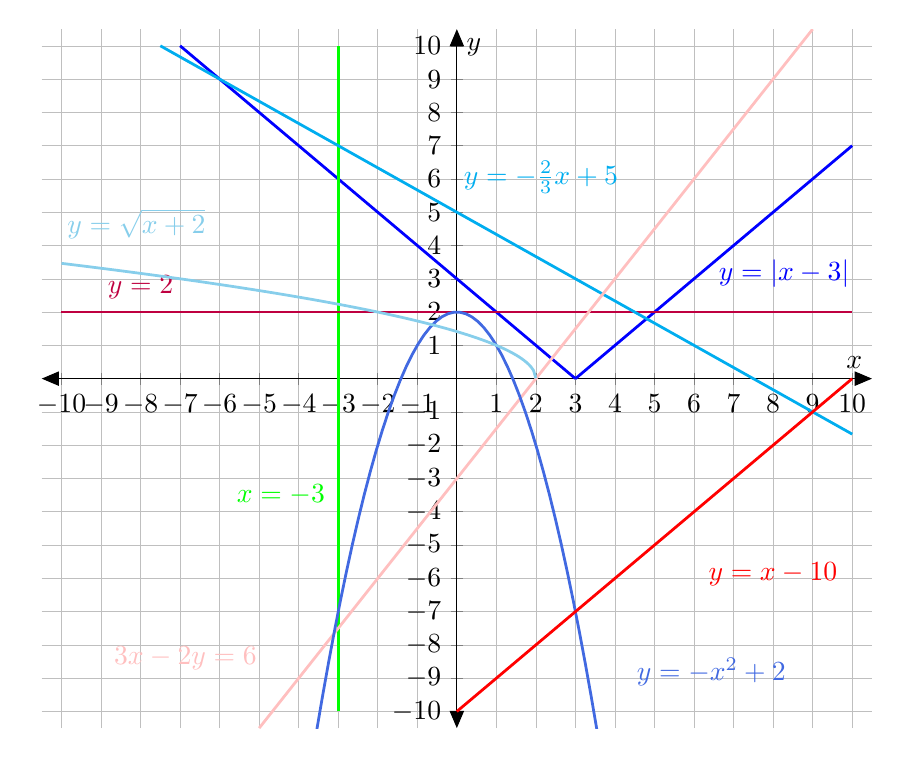
\begin{tikzpicture}[>=triangle 45]
        \begin{axis}[width=\linewidth,axis lines=center,axis line style={<->},
            xtick distance=1,xlabel = $x$,xmin=-10.5,xmax=10.5,ytick distance=1,ylabel = $y$,ymin=-10.5,ymax=10.5,
            grid=both,grid style={line width=.1pt, draw=gray!10},major grid style={line width=.2pt,draw=gray!50}]
            \addplot[domain=3:10,draw=blue,samples=3,line width=1pt,variable=\x] {\x-3)} node[pos=.45,right=3pt] {$\color{blue}y=|x-3|$};
            \addplot[domain=-7:3,draw=blue,samples=3,line width=1pt,variable=\x] {3-\x)};
            \addplot[domain=-10:10,draw=green,samples=3,line width=1pt,variable=\x] (-3,\x) node[pos=.325,left=1pt] {$\color{green}x=-3$};
            \addplot[domain=-10:10,draw=purple,samples=3,line width=1pt,variable=\x] {2} node[pos=.1,above=1pt] {$\color{purple}y=2$};
            \addplot[domain=-7.5:10,draw=cyan,samples=3,line width=1pt,variable=\x] {-0.6666666*\x+5} node[pos=.55,above=0.7cm] {$\color{cyan}y=-\frac{2}{3}x+5$};
            \addplot[domain=-5:9,draw=pink,samples=3,line width=1pt,variable=\x] {1.5*\x-3} node[pos=.1,left=0.6cm] {$\color{pink}3x-2y=6$};
            \addplot[domain=-3.7:3.7,draw=RoyalBlue,samples=50,line width=1pt,variable=\x] {-\x^2+2} node[pos=.9,right=0.5cm] {$\color{RoyalBlue}y=-x^{2}+2$};
            \addplot[domain=-10:2,draw=SkyBlue,samples=200,line width=1pt,variable=\x] {sqrt(2-\x)} node[pos=.15,above=0.3cm] {$\color{SkyBlue}y=\sqrt{x+2}$};
            \addplot[domain=0:10,draw=red,samples=3,line width=1pt,variable=\x] {\x-10} node[pos=.55,below right=0.3cm and 0.3cm] {$\color{red}y=x-10$};
        \end{axis}
    \end{tikzpicture}
    \caption{The chaos that is the solution to problem \ref{problem:north_shore_exam_graph_everything}}
    \label{fig:north_shore_graphing_problem}
\end{figure}
\subsection{Systems of Equations}
A system of equations is a set of 2 or more equations involving the same variables. Solving systems of linear equations is one of the main focuses in the study of linear algebra, and many techniques exists to solve these.
\begin{example}
\label{example:north_shore_example_of_a_system_of_linear_equations}Consider the following system of linear equations:
\begin{align*}
    2x+3y &=1\\
    x+6y &= 2
\end{align*}
Solving this system of equations asks ``Which ordered pairs $(x,y)$ solve both of these equations?" The second equations says that $x=2-6y$. We can substitute this back into the first equation to get $2(2-6y)+3y=1$ which simplifies to $4-9y = 1$. The solution to this is $y= \frac{1}{3}$. Solving for $x$, we have $x = 2 - 6y = 2 - 6(\frac{1}{3}) = 2-2 = 0$. $(0,\frac{1}{3})$ is a solution.
\end{example}
We can picture these types of problems graphically as well. For the example above there are two linear equations, which can be represented graphically as lines. A solution to this system can then be interpreted as a point where the two lines intersect. The graph of the two equations in example \ref{example:north_shore_example_of_a_system_of_linear_equations} are shown in Fig.~\ref{fig:north_shore_systems_of_linear_equations}.
\begin{figure}[H]
    \centering
    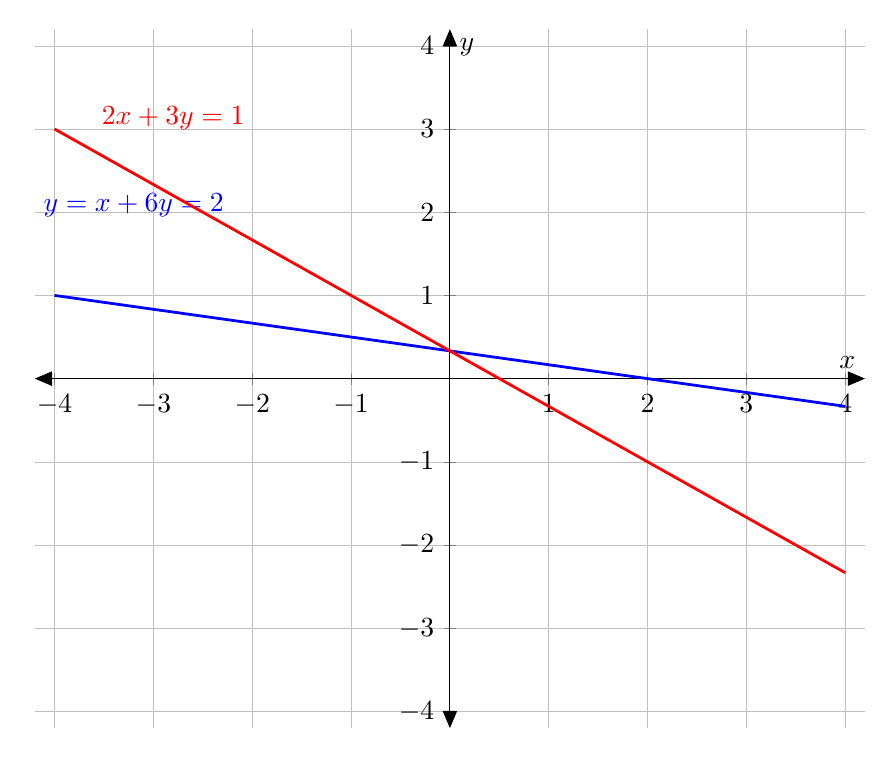
\begin{tikzpicture}[>=triangle 45]
        \begin{axis}[width=\linewidth,axis lines=center,axis line style={<->},
            xtick distance=1,xlabel = $x$,xmin=-4.2,xmax=4.2,ytick distance=1,ylabel = $y$,ymin=-4.2,ymax=4.2,
            grid=both,grid style={line width=.1pt, draw=gray!10},major grid style={line width=.2pt,draw=gray!50}]
            \addplot[domain=-4:4,draw=blue,samples=3,line width=1pt,variable=\x] {0.33333-0.16666*\x} node[pos=.1,above=1cm] {$\color{blue}y=x+6y=2$};
            \addplot[domain=-4:4,draw=red,samples=3,line width=1pt,variable=\x] {0.33333-0.66666*\x} node[pos=.15,above=0.7cm] {$\color{red}2x+3y=1$};
        \end{axis}
    \end{tikzpicture}
    \caption{The graphs of the two equations shown in example \ref{example:north_shore_example_of_a_system_of_linear_equations}.}
    \label{fig:north_shore_systems_of_linear_equations}
\end{figure}
Any system of linear equations has 3 possible outcomes: No solutions, one solution, or infinitely many solutions. This makes sense if one considers the few possibilities allowed. Given two parallel lines there will be no solutions for parallel lines never intersect. Given two equations that represent the same line there will be infinitely many solutions, for any point on the line will work. Given two equations for two distinct non-parallel lines there will be only one solution, for such lines can only intersect once.
\subsubsection{Problems}
\begin{problem}
Solve the following system of equations:
\begin{align*}
    2x-3y &= -12\\
    x-2y &= -9
\end{align*}
\end{problem}
\begin{proof}[Solution]
Subtracting 2 of the second equation from first equation, we get:
\begin{equation*}
    (2x-3y)-2(x-2y) = -12 - 2(-9)
\end{equation*}
Which simplifies to $y = 6$. The second equation yield $x -2(6) = -9\Rightarrow x = 3$. The solution is $(3,6)$
\end{proof}
\begin{problem}
Solve the following system of equations:
\begin{align*}
    4x+6y &= 10\\
    2x+3y &= 5
\end{align*}
\end{problem}
\begin{proof}[Solution]
Dividing both sides of the first equation by 2 gives us the second equation. These equations represent the same line, and there are infinitely many solutions: $y = \frac{5}{3} - \frac{2}{3}x$
\end{proof}
\begin{problem}
Solve the following system of equations:
\begin{align*}
    x+2y &= 5\\
    x+2y &= 7
\end{align*}
\end{problem}
\begin{proof}[Solution]
Let $z=x+2y$. Then $z=5$ and $z=7$. But this is impossible, for $5\ne 7$. No solutions.
\end{proof}
\begin{problem}
\begin{align*}
    2x-3y &= -4\\
    2x+\phantom{3}y &= \phantom{-}4
\end{align*}
\end{problem}
\begin{proof}[Solution]
Subtracting the first equation from the second gives us $4y = 8\Rightarrow y=2$. But then from the first equation we obtain $2x=3(2)-4 = 2\Rightarrow x=1$. The solution is $(1,2)$.
\end{proof}
\subsection{Radicals}
To simplify expressions with radicals we use something called the conjugate of a radical expression. 
\begin{definition}
The conjugate of a rational expression $\sqrt{a}-\sqrt{b}$ is $\sqrt{a}+\sqrt{b}$.
\end{definition}
Using the \gls{foil} rule from before, we can obtain the following theorem.
\begin{theorem}
If $a,b\geq 0$, and if $a\ne b$, then $\frac{1}{\sqrt{a}-\sqrt{b}} = \frac{\sqrt{a}+\sqrt{b}}{a-b}$
\end{theorem}
\begin{proof}
As $a,b\geq 0$ and $a\ne b$, $\frac{1}{\sqrt{a}-\sqrt{b}}$ is well-defined and $\sqrt{a}+\sqrt{b}\ne 0$. But then:
\begin{align*}
    \tfrac{1}{\sqrt{a}-\sqrt{b}} &= \tfrac{1}{\sqrt{a}-\sqrt{b}}\tfrac{\sqrt{a}+\sqrt{b}}{\sqrt{a}+\sqrt{b}}\\
    &= \tfrac{\sqrt{a}+\sqrt{b}}{(\sqrt{a}-\sqrt{b})(\sqrt{a}+\sqrt{b})}\\
    &= \tfrac{\sqrt{a}+\sqrt{b}}{a-b} & \tag{Thm.~\ref{theorem:north_shore_difference_of_squares}}
\end{align*}
\end{proof}
\subsubsection{Problems}
\begin{problem}
Simplify the following so that there are no radicals in the denominator:
\begin{enumerate}[itemsep=0pt]
\begin{multicols}{3}
    \item $\sqrt{8}\sqrt{10}$
    \item $\sqrt[4]{\frac{81}{x^4}}$
    \item $\sqrt{\frac{4}{3}}$
    \item $\sqrt{\frac{12}{18}}$
    \item $\sqrt[3]{24x^{3}y^{6}}$
    \item $\frac{\sqrt{3}}{5-\sqrt{3}}$
\end{multicols}
\end{enumerate}
\end{problem}
\begin{proof}[Solution]
\
\begin{enumerate}[itemsep=0pt]
\begin{multicols}{3}
    \item $\sqrt{8}\sqrt{10} = \sqrt{16\cdot 5} = 4\sqrt{5}$
    \item $\sqrt[4]{\frac{81}{x^4}} = \frac{3}{|x|}$
    \item $\sqrt{\frac{4}{3}} = \frac{2}{\sqrt{3}} = \frac{2\sqrt{3}}{3}$
    \item $\sqrt{\frac{12}{18}} = \frac{2\sqrt{3}}{3\sqrt{2}} = \frac{2\sqrt{2}\sqrt{3}}{6}$
    \item $\sqrt[3]{24x^{3}y^{6}} = 2\sqrt[3]{3}xy^{2}$
    \item $\frac{\sqrt{3}}{5-\sqrt{3}} = \frac{\sqrt{3}(5+\sqrt{3})}{5-3} = \frac{5\sqrt{3}+3}{2}$
\end{multicols}
\end{enumerate}
\end{proof}
\chapter{Calculus I}
\section{CLEP Exam}
\begin{problem}
    If $f(x)=-2x^{-3}$, then $f'(x)=$
    \begin{enumerate}[label=(\Alph*)]
        \begin{multicols}{4}
            \item Bob
            \item Bill
            \item Alice
            \item George
        \end{multicols}
    \end{enumerate}
\end{problem}
\section{Exam I}
\begin{problem}
Compute the derivative of $y(x) = \frac{1}{2}(x^{4}+7)$
\end{problem}
\begin{proof}[Solution]
$\frac{dy}{dx} = \frac{d}{dx}\big(\frac{1}{2}(x^{4}+7)\big) = \frac{1}{2}\frac{d}{dx}(x^{4}+7) = \frac{1}{2}(4x^{3}) = 2x^{4}$
\end{proof}
\begin{problem}
Compute the derivative of $y(x)=\frac{x^{2}+1}{5}$
\end{problem}
\begin{proof}[Solution]
$\frac{dy}{dx} = \frac{d}{dx}(\frac{x^{2}+1}{5}) = \frac{1}{5}\frac{d}{dx}(x^{2}+1) = \frac{1}{5}(2x) = \frac{2x}{5}$
\end{proof}
\chapter{Calculus II}
\chapter{Calculus III}
\chapter{Differential Equations}
\chapter{Linear Algebra I}
\chapter{Linear Algebra II}
\section{Miscellaneous Lecture Notes}
\subsection{Orthogonal Projections}
\begin{definition}
The span of $\mathcal{W}=\{X_{i}\}_{1}^{k} \subset \mathbb{R}^n$ is the set $\Span(\mathcal{W})=\{\sum_{i=1}^{k} a_i X_i: a_i \in \mathbb{R}\}$.
\end{definition}
\begin{definition}
A linearly dependent subset of $\mathbb{R}^{n}$ is a subset $S\subset\mathbb{R}^{n}$ such that there exists a finite subset $\{X_{i}\}_{i=1}^{k}\subset S$ and a subset $\{a_{i}\}_{i=1}^{k}\subset \mathbb{R}\setminus \{0\}$ such that $\sum_{i=1}^{k}a_{i}X_{i}=\mathbf{0}$
\end{definition}
\begin{definition}
A linearly independent subset of $\mathbb{R}^{n}$ is a subset $S\subset \mathbb{R}^{n}$ that is not linearly dependent.
\end{definition}
\begin{theorem}
If $S\subset\mathbb{R}^{n}$ is linearly independent, then $|S|\leq n$.
\end{theorem}
\begin{theorem}
If $\mathcal{W}\subset\mathbb{R}^{n}$ is linearly independent and $|\mathcal{W}| = k$, then $\Span(\mathcal{W})$ is a $k$ dimensional subspace of $\mathbb{R}^n$.
\end{theorem}
If we are a linearly independent subset $\mathcal{W}=\{X_1,\hdots, X_k\}\subset\mathbb{R}^n$, and some other vector $Y$, we may wish to consider the orthogonal projection of $Y$ onto the $k$ dimensional subspace spanned by $\mathcal{W}$. That is, we may wish to find a vector $Y'\in\Span(X_1,\hdots, X_k)$ such that $Y-Y'$ is orthogonal to $\Span(X_1,\hdots, X_k)$.
\begin{theorem}
If $\{X_1,\hdots, X_k\}\subset\mathbb{R}^n$ is linearly independent, $\mathcal{W} = \Span(X_1,\hdots, X_n)$, and if $Y\in \mathbb{R}^n$ is such that $Y\perp X_i$ for $i=1,2,\hdots, k$, then $\forall_{Z\in \mathcal{W}}$, $Y\perp Z$.
\end{theorem}
\begin{proof}
For let $Y\in \mathbb{R}^n$ be such that for $i=1,2,\hdots, k$, $Y\perp X_i$. Let $Z\in \mathcal{W}$. Then $Z= \sum_{i=1}^{k} a_i X_i$, where $a_i\in \mathbb{R}$. But then $\langle Y, Z\rangle = \sum_{i=1}^{k} a_i \langle Y, X_i\rangle = \sum_{i=1}^{k} a_i\cdot 0 = 0$. 
\end{proof}
\begin{lemma}
If $P$ is an $n\times k$ matrix whose columns are linearly independent, then $P^TP$ is invertible.
\end{lemma}
\begin{proof}
Suppose $P^TPX = 0$. Then $PX$ is orthogonal to the columns of $P$. But $PX$ is a linear combination of the columns of $P$, and thus $PX$ must be orthogonal to itself. Therefore $PX = 0$. But as the columns of $P$ are linearly independent, if $PX = 0$, then $X=0$. Thus $P^TPX = 0$ if and only if $X=0$. Therefore $P^TP$ is invertible.
\end{proof}
So we need $X_i^T(Y-Y') = 0$. Let $X_i = (x_{1i},x_{2i},\hdots, x_{ni})^{T}$ and let $P = (x_{ij})$. Then we have $P^T(Y-Y') = 0$, or $P^TY = P^T Y'$. But $Y'\in \mathcal{W}$, so $Y' = \sum_{i=1}^{k} c_i X_i = P(c_1,\hdots, c_k)^T = PC$. So we have $P^TY = P^TPC$, and thus $C = (P^TP)^{-1}P^TY$. Therefore $Y'=P(P^TP)^{-1}P^T Y$.
\begin{definition}
The projection matrix of $\Span(X_{1},\hdots,X_{k})$ is $P(P^TP)^{-1}P^T$, where $P=(x_{ij})$.
\end{definition}
\begin{theorem}
If $Q = P(P^TP)^{-1}P^T$ is a projection matrix for a subspace $\mathcal{W}$, then $Q^T =Q$.
\end{theorem}
\begin{proof}
    \begin{align*}
        Q^T &= \big(P(P^TP)^{-1}P^T\big)^T & &= P\big((P^TP)^T\big)^{-1}P^T\\
        &= (P^T)^T\big(P(P^TP)^{-1}\big)^T & &= P(P^TP)^{-1}P^T\\
        &= P\big((P^TP)^{-1}\big)^TP^T & &= Q\\
    \end{align*}
\end{proof}
\begin{theorem}
If $Q = P(P^TP)^{-1}P^T$ is a projection matrix for a subspace $\mathcal{W}$, then $Q^2 = Q$.
\end{theorem}
\begin{proof}
    \begin{align*}
        Q^2 &= QQ & &=P(P^TP)^{-1}P^T\\
        &= P(P^TP)^{-1}P^T P(P^TP)^{-1}P^T & &= Q\\
        &= P\big((PT^TP)^{-1}(P^TP)\big)(P^TP)^{-1}P^T
    \end{align*}
\end{proof}
\begin{theorem}
If $Q$ is an $n\times n$ matrix, $Q = Q^{2}$, and $Q=Q^{T}$, then there is a subspace $\mathcal{W}\subset \mathbb{R}^{n}$ such that $Q$ is the projection matrix of $\mathcal{W}$.
\end{theorem}
\subsection{Reflections}
Let $\mathcal{W}$ be a plane passing through the origin, and suppose we want to reflect a vector $v$ across this plane. Let $u$ be a unit vector along $\mathcal{W}^{\perp}$. That is, $u$ is normal to the plane. The projection of $v$ along the line through $u$ is then given by $\hat{v} = Proj_{u}(v) = u(u^Tu)^{-1}u^Tv$. But $u$ is a unit vector, and therefore $u^Tu = 1$, so $\hat{v} = uu^T v$. Let $Q_u = uu^T$. The definition of the reflection of $v$ across $\mathcal{W}$ is the vector $\Refl_{\mathcal{W}}(v)$ such that has the same magnitude as $v$ lying on the opposite side of $\mathcal{W}$. Thus $v-\Refl_{\mathcal{W}}(v) = 2Q_u v$, and so we have:
\begin{equation*}
    \Refl_{\mathcal{W}}(v) = v-2Q_u v = (I-2Q_u)v =(I-2uu^T)v
\end{equation*}
\begin{definition}
$H_{\mathcal{W}} = I-2uu^T$ is called the Reflection (Householder) Matrix for $\mathcal{W}$.
\end{definition}
\begin{definition}
An orthogonal matrix is a matrix $P$ such that $P^TP = I$.
\end{definition}
\subsection{Lecture Notes on Orthogonal Matrices}
\begin{definition}
An orthoganal matrix is a $n\times n$ matrix $A$ such that $A^{T}A = I$.
\end{definition}
\begin{theorem}
If $A$ is an orthogonal matrix, then $A^T = A^{-1}$.
\end{theorem}
\begin{proof}
For $A^TA = I$, and inverses are unique. Thus $A^T = A^{-1}$.
\end{proof}
If we let $A_{i} = Ae_{i}$, then $A^TA = (A_{i}^{T}A_{j}) = I$. Therefore $A_i^TA_j = \delta_{ij}$.
\begin{theorem}
If $A$ is an $n\times n$ real-valued matrix and $A_i = Ae_i$, $i=1,2,\hdots, n$, then $A$ is orthogonal if and only if $\{A_1,\hdots, A_n\}$ is an orthonormal set of vectors.
\end{theorem}
\begin{proof}
If $A$ is orthogonal, then $A_{i}^{T}A_{j} = \delta_{ij}$, and from this we have orthonormality. If $\{A_1,\hdots, A_n\}$ is orthonormal, then $A^TA = I$ and is therefore orthogonal.
\end{proof}
\begin{theorem}
The following statements are equivalent:
\begin{enumerate}
\begin{multicols}{3}
    \item $A$ is orthogonal
    \item $\forall_{X\in\mathbb{R}^{n}}$, $\norm{AX} = \norm{X}$
    \item $\forall_{X,Y\in\mathbb{R}^{n}}$, $\langle AX, AY\rangle = \langle X, Y\rangle$
\end{multicols}
\end{enumerate}
\end{theorem}
\begin{proof}
We show $1\Rightarrow 2 \Rightarrow 3 \Rightarrow 1$.
\begin{enumerate}[itemsep=0pt]
\item If $A$ is orthogonal, then $A^TA = I$. But then we have:
    \begin{equation*}
        \norm{AX}^{2}=(AX)^{T}AX=(X^{T}A^{T})AX=X^{T}(A^{T}A)X=X^{T}IX=X^{T}X=\norm{X}^{2}
    \end{equation*}
    Therefore $\norm{AX} = \norm{X}$.
\item If $A$ is a square matrix such that $\forall_{X\in\mathbb{R}^{n}}$, $\norm{AX} = \norm{X}$, then:
    \begin{equation*}
        \norm{X+Y}^{2}=(X+Y)^T(X+Y)=X^TX+X^TY+Y^TX+Y^TY=\norm{X}^2+2X^TY+\norm{Y}^2
    \end{equation*}
    But:
    \begin{equation*}
        \norm{A(X+Y)}^{2}=\norm{AX+AY}^{2}=\norm{AX}^{2}+2(AX)^{T}AY+\norm{AY}^2=\norm{X}^{2}+2(AX)^{T}AY+\norm{Y}^2
    \end{equation*}
    Therefore $(AX)^TAY = X^TY$. That is, $\langle AX, AY\rangle = \langle X, Y\rangle$.
    \item If $A$ is a square matrix such that $\forall_{X,Y\in \mathbb{R}^n}$, $\langle AX, AY\rangle = \langle X, Y\rangle$, and $A_i =  Ae_i$, then:
        \begin{equation*}
            A_{i}^{T}A_{j}=\langle Ae_{i}, Ae_{j}\rangle=(Ae_{i})^{T}Ae_{j}=\langle e_i,e_j\rangle=\delta_{ij}
        \end{equation*}
        Therefore, $A$ is orthogonal.
\end{enumerate}
\end{proof}
\begin{theorem}
If $A$ and $B$ are $n\times n$ orthogonal matrices, then $AB$ is orthogonal.
\end{theorem}
\begin{proof}
For if $A^{T}A = I$ and $B^{T}B = I$, then $(AB)^{T}AB = B^{T}A^{T}AB = B^{T}IB = B^{T}B = I$. $AB$ is orthogonal.
\end{proof}
\begin{theorem}
\label{theorem:LINEAR_ALGEBRA_orthogonal_matrices_have_determinant_pm_1}
If $A$ is an $n\times n$ orthogonal matrix, then $\det(A) = 1$ or $-1$.
\end{theorem}
\begin{proof}
For $\det(I) = \det(A^TA) = \det(A^T)\det(A) = \det(A)^2$. Thus, $\det(A) = \pm 1$.
\end{proof}
\begin{remark}
The converse of Thm.~\ref{theorem:LINEAR_ALGEBRA_orthogonal_matrices_have_determinant_pm_1} is false.
\end{remark}
Recall that if $u\in \mathbb{R}^n$ is a unit vector and $W = u^{\perp}$, then $H=2uu^T$ is the reflection matrix for $W$. Reflections preserve distance, and therefore $H$ must be orthogonal.
\begin{theorem}
If $A$ is an $n\times n$ orthogonal matrix, then there exist $k$ $n\times n$ reflection matrices $H_1,\hdots, H_k$, $0\leq k \leq n$, such that $A = \prod_{i=1}^{j}H_i$.
\end{theorem}
\begin{proof}
By induction. The base case is trivial. Suppose it holds for $n-1$. Let $z = Ae_n$, and let $H$ be the reflection matrix that exchanges $z$ and $e_n$. Then $HAe_n = Hz = e_n$, so $HA$ fixes $e_n$. But $HA$ is an orthogonal matrix, and thus preserves distances and angles. Thus $HA$ maps $\mathbb{R}^{n-1}$ onto itself, and thus by induction there are $H_2,\hdots, H_k$ such that $HA = \prod_{i=2}^{k} H_i$. Letting $H_{1}=H$, we have $A = HHA = \prod_{i=1}^{k}H_i$.
\end{proof}
\begin{theorem}
If $H$ is a reflection matrix, then $\det(H) = -1$.
\end{theorem}
\begin{theorem}
If $A$ is an orthogonal matrix and $A=\prod_{i=1}^{k} H_i$, then $\det(A) = (-1)^k$.
\end{theorem}
If $A$ is an orthogonal $2\times 2$ matrix, then we know that columns must be unit vectors that are also orthogonal (Orthonormal). That is, the two columns must lie on the unit circle about the origin. So we may express the first column as $(\cos(\theta),\sin(\theta))$ for some angle $\theta$. There are then two options for the seconds column: $(-\sin(\theta),\cos(\theta))$ or $(\sin(\theta),-\cos(\theta))$. The first is the rotation matrix which rotates $\mathbb{R}^2$ counterclockwise around the origin, and the second is the reflection matrix that makes a reflection across the line that makes an angle $\frac{\theta}{2}$ with the $x-$axis. 
\begin{theorem}
If $A$ is a $3\times 3$ orthogonal matrix, then one of the following is true:
\begin{enumerate}[itemsep=0pt]
\item If $\det(A) = 1$, then $A$ is a rotation matrix.
\item If $\det(A) = -1$ and $A=A^T$, then either $A=-I$ or $A$ is a reflection matrix.
\item If $\det(A) = -1$ and $A\ne A^T$, then $A$ is the product of three reflections.
\end{enumerate}
\end{theorem}
\begin{proof}
$A$ must be the product of $0,1,2,$ or $3$ reflection matrices. If $\det(A) = 1$, then $A$ is the product of an even number of reflections, and thus either $A=I$ or $A$ is the product of two reflections, and is thus a rotation. If $\det(A)=-1$, then $A$ is the product of an odd number of reflections, either $1$ or $3$. If $A$ is a single reflection, then $A=H$ for some Householder matrix $H$. Thus $A^T = A$. Conversely, if $A = A^T$ and $\det(A) = -1$, then $\det(-A) = 1$, and $-A^T = -A = -A^{-1}$. Therefore $-A$ is a rotation whose square is the identity. If $A\ne I$, then $A$ must be a rotation of $\pi/2$ around some axis, and thus $A$ is a reflection. If $\det(A) = -1$, and $A\ne A^T$, then $A$ cannot be a rotation or a pure reflection, and thus $A$ is the product of $3$ reflection matrices.
\end{proof}
\begin{theorem}
If $A$ and $B$ are $3\times 3$ rotation matrices, then $AB$ is a rotation matrix.
\end{theorem}
\begin{proof}
For $A$ and $B$ must be orthogonal, and thus $AB$ is orthogonal. But $\det(AB) = \det(A)\det(B) = 1\cdot 1 = 1$, and thus $AB$ is an orthogonal matrix with determinant equal to $1$, and is therefore a rotation matrix.
\end{proof}
\subsection{Rotations}
The $2\times 2$ matrix $A_{\theta}$ rotates the plane $\mathbb{R}^2$ counterclockwise by $\theta$ around the origin. It is defined by:
\begin{equation*}
    A_{\theta}=\begin{bmatrix*}[r]\cos(\theta) & -\sin(\theta) \\ \sin(\theta) & \cos(\theta)\end{bmatrix*}
\end{equation*}
The question that then arises is, ``Is there a similar way to do this for $\mathbb{R}^3$?" The simple case would be rotating by an angle $\theta$ about the $z-$axis, analogous the rotating the Earth by $\theta$ about the North Pole. This fixes the $z-$axis and acts on the $xy$ plane only. This can be represented by the matrix:
\begin{equation*}
 S_{\theta} = \begin{bmatrix*} \cos(\theta) & -\sin(\theta) & \phantom{sin}0 \\ \sin(\theta) & \phantom{-}\cos(\theta) & \phantom{sin}0\\ 0 & \phantom{-}0 & \phantom{sin}1 \end{bmatrix*}   
\end{equation*}
$S_{\theta}$ is an orthogonal matrix. That is, $S_{\theta} S_{\theta}^T = I$, and therefore $S_{\theta}^T = S_{\theta}^{-1}$. Suppose we want to rotate by an angle $\theta$ about a different axis. Let $\mathbf{u}$ be a unit vector pointing in the direction of the axis of rotation and let $R_{\theta,\mathbf{u}}$ be the new rotation matrix. To compute $R_{\theta,\mathbf{u}}$ we need to choose a unit vector $\mathbf{v}$ that is orthogonal to $\mathbf{u}$. Let $\mathbf{w} = \mathbf{u}\times \mathbf{v}$. Then $\{\mathbf{u},\mathbf{v},\mathbf{w}\}$ is an orthonormal basis of $\mathbb{R}^3$ such that $\mathbf{v}\times \mathbf{w} = \mathbf{u}$. Let:
\begin{equation*}
    P = \begin{bmatrix} v_1 & w_1 & u_1 \\ v_2 & w_2 & u_2 \\ v_3 & w_3 & u_3 \end{bmatrix}
\end{equation*}
The columns of $P$ form an orthonormal set, and therefore $P$ is orthogonal. In particular:
\begin{align*}
    P^{T}\mathbf{v} &= e_{1} & P^{T}\mathbf{w} &= e_{2} & P^{T}\mathbf{u} &= e_{3}
\end{align*}
\begin{theorem}
If $\theta \in [0,2\pi]$ and $\mathbf{u}\in \mathbb{R}^3$ is a unit vector, then $R_{\theta, \mathbf{u}} = PS_{\theta}P^T$.
\end{theorem}
\begin{proof}
For:
\begin{align*}
    PS_{\theta}P^T\mathbf{u} &= P(0,0,1)^{T}=\mathbf{u}\\
    PS_{\theta}P^{T}\mathbf{v} &= \cos(\theta)\mathbf{v}+\sin(\theta) \mathbf{w}\\
    PS_{\theta}P^{T} \mathbf{w} &= -\sin(\theta) \mathbf{v}+\cos(\theta) \mathbf{w}
\end{align*}
Thus, if $X = a\mathbf{v}+b\mathbf{w}+c\mathbf{u}$, then:
\begin{equation*}
    PS_{\theta}P^TX=a(\cos(\theta)\mathbf{v}+\sin(\theta)\mathbf{w})+b(-\sin(\theta)\mathbf{v}+\cos(\theta)\mathbf{w})+c\mathbf{u}=R_{\theta,\mathbf{u}}X
\end{equation*}
\end{proof}
From the orthogonality of $P$ and $S_{\theta}$ we have that $R_{\theta,\mathbf{u}}$ is also orthogonal.
\begin{theorem}
\label{theorem:LINEAR_ALGEBRA_a_rotation_matrix_is_an_orthoganal_matrix_with_determinant_1}
A rotation matrix $R$ is an orthogonal matrix with determinant $1$.
\end{theorem}
\begin{proof}
For:
\begin{equation*}
    R^{T}R=(PS_{\theta}P^{T})^{T}PS_{\theta}P^{T}=(PS_{\theta}^{T}P^{T})PS_{\theta}P^{T}=PS_{\theta}^{T}(P^{T}P)S_{\theta}P^{T}=PS_{\theta}^{T}S_{\theta}P^{T}=PP^{T}=I
\end{equation*}
And
\begin{align*}
    \det(R) &=\det(PS_{\theta}P^T)=\det(P)\det(S_{\theta})\det(P^T)=\det(P)\det(S_{\theta})\det(P^{-1})\\
    &=\det(P)\det(S_{\theta})\tfrac{1}{\det(P)}=\det(S_{\theta})= 1
\end{align*}
\end{proof}
\begin{remark}
The converse of Thm.~\ref{theorem:LINEAR_ALGEBRA_a_rotation_matrix_is_an_orthoganal_matrix_with_determinant_1} is also true.
\end{remark}
We now turn to the question of how to compute the rotation of $\mathbb{R}^3$ represented by a given orthogonal matrix. If $R$ is an orthogonal matrix such that $\det(R) = 1$, how do we compute the angle of rotation? First recall that the trace of a matrix is the sum of the diagonal components, $\Tr(A) = \sum_{i=1}^{n}a_{ii}$.
\begin{theorem}
If $A$ and $B$ are $n\times n$ matrices, then $\Tr(AB) = \Tr(BA)$
\end{theorem}
\begin{theorem}
If $R$ is a rotation matrix of angle $\theta$, then $\cos(\theta) = \frac{\Tr(R) - 1}{2}$.
\end{theorem}
\begin{proof}
Since $R = PS_{\theta} P^T = PS_{\theta}P^{-1}$, we have:
\begin{equation*}
    \Tr(R) = \Tr(PS_{\theta}P^{-1}) = \Tr(PP^{-1}S_{\theta}) = \Tr(S_{\theta}) = 1+2\cos(\theta)\Rightarrow \cos(\theta) = \tfrac{\Tr(R)-1}{2}
\end{equation*}
\end{proof}
This doesn't tell us everything, as we still don't know $\mathbf{u}$, and $\cos(\theta) = \cos(-\theta)$, so we still don't know the sign of $\theta$. Since $R$ is an orthogonal matrix, $R^T = R^{-1}$. So if $\mathbf{u}$ lies on the axis of rotation, then $(R-R^T)\mathbf{u} = R\mathbf{u}-R^{-1}\mathbf{u} = \mathbf{u}-\mathbf{u} = 0$. We can find the axis of rotation by determining the null space of $R-R^T$. 
\begin{equation*}
    R = \begin{bmatrix*}[c] r_{11} & r_{12} & r_{13} \\ r_{21} & r_{22} & r_{23} \\ r_{31} & r_{32} & r_{33} \end{bmatrix*} \Rightarrow R-R^{T} = \begin{bmatrix*}[c] 0 & r_{12} - r_{21} & r_{13} - r_{31} \\ r_{21} - r_{12} & 0 & r_{23}-r_{32} \\ r_{31} - r_{13} & r_{32} - r_{23} & 0 \end{bmatrix*}
\end{equation*}
Let $\alpha = r_{12} - r_{21},\beta = r_{13} - r_{31},$ and $\gamma = r_{23}-r_{32}$. Then:
\begin{equation*}
    R-R^T = \begin{bmatrix*}[r] 0 & \alpha & \beta \\ -\alpha & 0 & \gamma \\ -\beta & -\gamma & \phantom{-}0 \end{bmatrix*}
\end{equation*}
This suggests that $\mathbf{u}$ is parallel to $(-\gamma, \beta, -\alpha)^{T} = (r_{32}-r_{23}, r_{13}-r_{31}, r_{21}-r_{12})^{T}$.
\begin{theorem}
If $R$ is a rotation matrix such that $R\ne R^T$, then the axis of rotation of $R$ is parallel to $\mathbf{q}=(-\gamma, \beta, -\alpha)^{T} = 2\sin(\theta)\mathbf{u}$, where $\mathbf{u}$ is a unit vector about the axis of rotation.
\end{theorem}
\begin{proof}
Let $R = PS_{\theta}P^T$. Then:
\begin{equation*}
    R-R^{T}=PS_{\theta}P^{T}-PS_{\theta}^{T}P^{T}=P(S_{\theta}-S_{\theta}^{T})P^{T}=2P\begin{bmatrix}0 & -\sin(\theta) & 0 \\ \sin(\theta) & 0 & 0 \\ 0 & 0 & 0 \end{bmatrix}P^{T}= 2\sin(\theta)(\mathbf{w}\mathbf{v}^{T} - \mathbf{v}\mathbf{w}^{T})
\end{equation*} 
Where $\mathbf{v}$ is orthogonal to $\mathbf{u}$ and $\mathbf{w} = \mathbf{u}\times \mathbf{v}$. Therefore:
\begin{equation*}
    \mathbf{q} = (-\gamma, \beta, -\alpha)^{T} = 2\sin(\theta) \mathbf{v}\times \mathbf{w} = 2\sin(\theta) \mathbf{u}
\end{equation*}
\end{proof}
\begin{remark}
What about the case when $R-R^T = 0$? When this happens either $\theta = 0$ or $\theta = \pi$. If $\theta = 0$, then this is the identity rotation and thus $R = I$, and we are done. If $R\ne I$, then $\theta = \pi$. To find out the axis of rotation, we have that:
\begin{equation*}
    R = PS_{\pi}P^T = \begin{bmatrix*}[r]-1 & 0 & \phantom{-}0 \\ 0 & -1 & 0 \\ 0 & 0 & 1 \end{bmatrix*} = -\mathbf{v}\mathbf{v}^T-\mathbf{w}\mathbf{w}^T +\mathbf{u}\mathbf{u}^T    
\end{equation*}
But $\mathbf{v},\mathbf{w},$ and $\mathbf{u}$ form an orthonormal basis, and therefore $\mathbf{v}\mathbf{v}^T + \mathbf{w}\mathbf{w}^T+\mathbf{u}\mathbf{u}^T = I$. Thus, $R = -I+2\mathbf{u}\mathbf{u}^T$, so $\mathbf{u} \mathbf{u}^T = \frac{1}{2}(R+I)$. But the columns of $\mathbf{u}\mathbf{u}^T$ are parallel to $\mathbf{u}$, and therefore we can determine $\mathbf{u}$ by normalizing one of the columns of $\frac{1}{2}(R+I)$.
\end{remark}
\subsection{The Matrix Exponential}
\begin{definition}
If $A$ is an $n\times n$ matrix, then the exponential of $A$ is $e^{A} =\sum_{k=0}^{\infty} \frac{A^k}{k!}$.
\end{definition}
\begin{remark}
Notationally, we write $A^0 = I$. For any complex-valued matrix $A$ of finite dimension, it can be shown that this sum converges.
\end{remark}
\begin{theorem}
If $A$ and $P$ are complex $n\times n$ matrices and $P$ is an $n\times n$ invertible matrix, then $e^{P^{-1}AP} = P^{-1}e^{A}P$.
\end{theorem}
\begin{proof}
For all $m\in \mathbb{N}$, $(P^{-1}AP)^{m} = P^{-1}A^mP$. Thus:
\begin{equation*}
    e^{P^{-1}AP} = \sum_{k=0}^{\infty} P^{-1}\frac{A^k}{k!}P = P^{-1}\big(\sum_{k=0}^{\infty} \frac{A^k}{k!}\big)P = P^{-1}e^A P
\end{equation*}
\end{proof}
\begin{theorem}
If $0$ is the zero matrix, then $e^0 = I$.
\end{theorem}
\begin{theorem}
If $A$ is an $n\times n$ matrix and $m\in \mathbb{N}$, then $A^{m} e^{A} = e^{A} A^{m}$.
\end{theorem}
\begin{proof}
For $A^{m} e^{A} = A^{m} \sum_{k=0}^{\infty} \frac{A^{k}}{k!} = \sum_{k=0}^{\infty} \frac{A^{k+m}}{k!} = \big(\sum_{k=0}^{\infty} \frac{A^k}{k!}\big)A^{m}$.
\end{proof}
\begin{theorem}
If $A$ is an $n\times n$ matrix, then $e^{A^{T}} = (e^{A})^{T}$.
\end{theorem}
\begin{proof}
For $e^{A^{T}} = \sum_{k=0}^{\infty} \frac{(A^{T})^{k}}{k!} = \sum_{k=0}^{\infty} \frac{(A^{k})^{T}}{k!} = \big(\sum_{k=0}^{\infty} \frac{A^{k}}{k!}\big)^{T} = (e^{A})^{T}$.
\end{proof}
\begin{theorem}
If $A$ and $B$ are $n\times n$ matrices and if $AB = BA$, then $Ae^{B} = e^{B} A$.
\end{theorem}
\begin{proof}
For $Ae^{B} = A\sum_{k=0}^{\infty} \frac{B^{k}}{k!} = \sum_{k=0}^{\infty} A\frac{B^{k}}{k!} = \sum_{k=0}^{\infty} \frac{B^{k}}{k!}A = \big(\sum_{k=0}^{\infty} \frac{B^{k}}{k!}\big)A = e^{B}A$.
\end{proof}
\begin{theorem}
If $A$ and $B$ are $n\times n$ matrices and $AB = BA$, then $e^{A}e^{B} = e^{B}e^{A}$.
\end{theorem}
\begin{proof}
For:
\begin{align*}
    e^A e^B &= e^A\sum_{k=0}^{\infty}\frac{B^k}{k!}=\sum_{k=0}^{\infty} e^A\frac{B^k}{k!}= \sum_{k=0}^{\infty} \big(\sum_{j=0}^{\infty} \frac{A^j}{j!}\big) \frac{B^k}{k!}= \sum_{k=0}^{\infty}\big(\sum_{j=0}^{\infty} \frac{A^j}{j!}\frac{B^k}{k!}\big)\\
    &=\sum_{k=0}^{\infty}\big(\sum_{j=0}^{\infty} \frac{B^k}{k!}\frac{A^j}{j!}\big)=\sum_{k=0}^{\infty}\big(\sum_{j=0}^{\infty} \frac{B^k}{k!}\big)\frac{A^j}{j!}= \sum_{k=0}^{\infty}\frac{B^k}{k!}\sum_{j=0}^{\infty}\frac{A^j}{j!}=e^{B}e^{A}
\end{align*}
\end{proof}
It is NOT true that $e^{A+B}=e^{A}e^{B}$, in general. Matrix exponentiation lacks this feature.
\begin{theorem}
If $A$ is an $n\times n$ matrix and $s,t\in \mathbb{C}$, then $e^{A(s+t)} = e^{As}e^{At}$.
\end{theorem}
\begin{proof}
For $e^{As}e^{At} = \sum_{j=0}^{\infty} \sum_{k=0}^{\infty} \frac{A^{j+k}s^jt^k}{j!k!}$. Letting $n = j+k$, so $j = n-k$, we have:
\begin{equation*}
    \sum_{n=0}^{\infty} \sum_{k=0}^{\infty} \frac{A^n}{n!}\frac{n!}{k!(n-k)!}s^{n-k}t^k = \sum_{n=0}^{\infty}\frac{A^n}{n!}\big(\sum_{k=0}^{\infty} \frac{n!}{k!(n-k)!}s^{n-k}t^k\big)    
\end{equation*}
From the binomial theorem, the expression inside the parenthesis is equal to $(s+t)^n$. So we have $e^{As}e^{At}=\sum_{n=0}^{\infty} \frac{A^n(t+s)^n}{n!} = e^{A(s+t)}$.
\end{proof}
\begin{theorem}
If $A$ is an $n\times n$ matrix, then $e^A$ is invertible and $(e^A)^{-1} = e^{-A}$.
\end{theorem}
\begin{proof}
For $I = e^{0} = e^{A(1-1)} = e^Ae^{-A}$. Thus $(e^{A})^{-1} = e^{-A}$.
\end{proof}
\begin{theorem}
If $A$ is an $n\times n$ matrix and $t\in \mathbb{R}$, then $\frac{d}{dt}\big(e^{At}\big) = Ae^{At}$.
\end{theorem}
\begin{proof}
For $\underset{h\rightarrow 0}\lim \frac{e^{A(t+h)}-e^{At}}{h} = e^{At}\underset{h\rightarrow 0}\lim \frac{e^{Ah}-I}{h} = e^{At}\underset{h\rightarrow 0}\lim\big[A+\frac{A^2}{2!}h+\hdots\big] = e^{At}A = Ae^{At}$.
\end{proof}
\begin{theorem}
If $A$ and $B$ are $n\times n$ matrices and $AB=BA$, then $e^{A+B} = e^{A}e^{B}$.
\end{theorem}
\begin{proof}
For let $g(t) = e^{(A+B)t}e^{-Bt}e^{-At}$. Then from commutativity of $A$ and $B$, $g'(t) = 0$. But then $g(t)$ is a constant. From the definition, $g(0) = I$, and thus $g(t) = I$. So $e^{(A+B)t}e^{-Bt}e^{-At} = I$, and therefore $e^{(A+B)t} = e^{At}e^{Bt}$.
\end{proof}
\begin{theorem}
If $A^{2} = 0$, then $e^{A} = I+A$.
\end{theorem}
\begin{proof}
For $e^{A} = I+A+A^{2}\big(\frac{I}{2!}+\frac{A}{3!}+\hdots\big) = I+A+0 = I+A$.
\end{proof}
\subsection{Linear Systems of Ordinary Differential Equations}
Consider the equation $y' = ky$, where $k$ is some constant. We can solve this via calculus using separation of variables:
\begin{equation*}
    \frac{y'}{y} = k\Rightarrow \int \frac{y'}{y}dx = \int kdx \Rightarrow \ln(y) = kx+c \Rightarrow y = e^c e^{kx}    
\end{equation*}
Setting $x=0$, we have $e^c = y_0$. So $y = y_0e^{kx}$. Let us solve this a different way: Let $F(x) = e^{-kx}y$, and let $y'=kx$. Differentiating we have:
\begin{equation*}
    F'(x)=-ke^{kx}y+e^{-kx}y'=-kye^{-kx}+e^{-kx}ky=0    
\end{equation*}
So $F'(x) = 0$, and therefore $F(x)$ is a constant. Setting $x=0$, we have $F(x) = y_0$. So $y = y_0e^{kx}$. This shows us that $y_0e^{kx}$ is the $only$ solution to this problem. Let:
\begin{equation*}
    Y(t) = \begin{bmatrix} y_1(t) \\ y_2(t)\end{bmatrix}    
\end{equation*}
Consider the system $Y'(t) = AY(t)$, where $A$ is an $n\times n$ matrix. Let $F(t) = e^{-At}Y(t)$. Then $F'(t) = 0$, and $Y(t) = Y_0 e^{At}$.
\begin{theorem}
If $Y:\mathbb{R}\rightarrow \mathbb{R}^n$ is a differentiable function such that $Y'(t) = AY(t)$, where $A$ is a diagonalizable matrix with eigenvalues $\lambda_1,\hdots, \lambda_n$ and eigenvectors $v_1,\hdots, v_n$, then $Y(t) = \sum_{k=1}^{n} \lambda_k e^{\lambda_k t}v_k$
\end{theorem}
\section{Problem Sets}
\subsection{Problem Set I}
\begin{problem}
Find the point on the line $y=4x$ which is closest to the point $(2,5)$.
\end{problem}
\begin{proof}[Solution 1]
Given a vector $\mathbf{v}$ that is parallel to the line $y$, we know that the vector $\mathbf{w}$ from $(2,5)$ to the point $(x,y)$ that minimizes the distance from $y=4x$ to the point $(2,5)$ will satisfy $\langle \mathbf{v}, \mathbf{w}\rangle = 0$. That is:
\begin{equation*}
    \big\langle (1,4), (2-x,5-y)\big\rangle = 0\Rightarrow 2-x+4(5-y) = 0 \Rightarrow 22 - x - 4 y = 0    
\end{equation*}
But $y = 4x$, and thus $22-17x = 0 \Rightarrow x= \frac{22}{17}$. The point of least distance is $\frac{22}{17}(1,4)$.
\end{proof}
\begin{proof}[Solution 2]
This point is the projection of the vector $(2,5)^T$ onto $(1,4)^T$. That is:
\begin{equation*}
    \mathbf{P} = \frac{\begin{bmatrix}2 & 5 \end{bmatrix} \begin{bmatrix} 1 \\ 4 \end{bmatrix}}{\begin{bmatrix} 1 & 4 \end{bmatrix} \begin{bmatrix} 1 \\ 4 \end{bmatrix}} \begin{bmatrix} 1 \\ 4 \end{bmatrix} = \frac{22}{17} \begin{bmatrix} 1 \\ 4\end{bmatrix}
\end{equation*}
\end{proof}
\begin{problem}
Show that $\mathbf{x}\mathbf{y}^T + \mathbf{y}\mathbf{x}^T$ is symmetric.
\end{problem}
\begin{proof}[Solution]
Recall that a matrix is symmetric if it is equal to its transpose. Thus, we must show $A = A^T$. But for any $n\times n$ matrices $A$ and $B$, $(A+B)^T = A^T + B^T$, and $(AB)^T = B^T A^T$, and $(A^T)^T = A$. Thus, given our matrix $A= \mathbf{x}\mathbf{y}^T + \mathbf{y}\mathbf{x}^T$, we have that $A^T = (\mathbf{x}\mathbf{y}^T + \mathbf{y}\mathbf{x}^T)^T = (\mathbf{x}\mathbf{y}^T)^T + (\mathbf{y}\mathbf{x}^T)^T = (\mathbf{y}^T)^T\mathbf{x}^T + (\mathbf{x}^T)^T\mathbf{y}^T = \mathbf{y}\mathbf{x}^T + \mathbf{x}\mathbf{y}^T = \mathbf{x}\mathbf{y}^T + \mathbf{y}\mathbf{x}^T = A$
\end{proof}
\begin{problem}
Compute the product $\begin{bmatrix*}[r] 2 & -1 \\ 3 & 1\end{bmatrix*} \begin{bmatrix*}[r] -1 & \phantom{-}2 & \phantom{-}3 & \phantom{-}1 \\ 2 & -2 & 1 & -1 \end{bmatrix*}$
\end{problem}
\begin{proof}[Solution]
\begin{align*}
    \begin{bmatrix*}[r] 2 & -1 \\ 3 & 1\end{bmatrix*} \begin{bmatrix*}[r] -1 & \phantom{-}2 & \phantom{-}3 & \phantom{-}1 \\ 2 & -2 & 1 & -1 \end{bmatrix*}&=\begin{bmatrix} 2(-1)+(-1)2 & 2\cdot 2 + (-1)(-2) & 2\cdot 3 + (-1)1 & 2\cdot 1 + (-1)(-1) \\ 3(-1)+1\cdot 2 & 3\cdot 2 + 1(-2) & 3\cdot 3 + 1\cdot 1 & 3\cdot 1 + 1(-1)\end{bmatrix}\\
    &=\begin{bmatrix} -4 & 6 & 5 &3 \\ -1 & 4 & 10 & 2\end{bmatrix}
\end{align*}
\end{proof}
\begin{problem}
Find the equation of the plane that contains $P_{1}(2,2,1),P_{2}(2,3,2)$, and $P_{3}(-1,3,1)$.
\end{problem}
\begin{proof}[Solution]
It suffices to find a vector normal to this plane. We have that:
\begin{equation*}
    \overrightarrow{P_1P_2} = (0,1,1)^T \quad\quad\quad\quad \overrightarrow{P_1P_3} = (-3,1,0)^T
\end{equation*}
Then both vectors are parallel to the plane, and thus $\overrightarrow{P_1P_2}\times \overrightarrow{P_1P_3}=(-1,3,3)^T$ is perpendicular to the plane. Suppose $Q=(x,y,z)$ is a point in the plane. Then the relative position vector $P_1 Q = (x-2,y-2,z-1)^T$ is orthogonal to $(-1,3,3)^T$. Thus:
\begin{align*}
    (x-2,y-2,z-1)(-1,3,3)^T &= 0\\
    \Rightarrow 2-x+3y-6+3z-3 &= 0\\
    \Rightarrow x-3y-3z +7 &= 0   
\end{align*}
This is the equation of the plane.
\end{proof}
\begin{problem}
Let $S$ be the subspace of $\mathbb{R}^3$ spanned by $\mathbf{x}_1 = (1,-1,2)^T$ and $\mathbf{x}_2 = (-1,2,2)^T$. Find a basis for $S^{\perp}$
\end{problem}
\begin{proof}[Solution]
We seek a vector in $\mathbf{x}_3\in\mathbb{R}^3$ such that $\langle \mathbf{x}_3, \mathbf{x}_{1,2}\rangle = 0$. Or in other words:
\begin{equation*}
    \begin{bmatrix*}[r] 1 & -1 & \phantom{-}2 \\ 0 & 1 & 4 \end{bmatrix*}\begin{bmatrix} x_1 \\ x_2 \\ x_3 \end{bmatrix} = 0    
\end{equation*}
This gives the following:
\begin{align*}
x_1 - x_2 + 2x_3 &= 0\\
	x_2 + 4x_3 &= 0
\end{align*}
So $x_2 = -4x_3$, $x_1=-6x_3$. Thus $\mathbf{x}_3 = x_3(-6,-4,1)^T$. $x_3$ is a free variable.
\end{proof}
\begin{problem}
For the matrix $A = \begin{bmatrix} 1 & 2 & 2 \\ -1 & -1 & 0 \end{bmatrix}$, find a basis for the following:
\begin{enumerate}
\begin{multicols}{4}
    \item $R(A^T)$
    \item $N(A)$
    \item $R(A)$
    \item $N(A^T)$
\end{multicols}
\end{enumerate}
\end{problem}
\begin{proof}[Solution] In order,
\begin{enumerate}[itemsep=0pt]
    \item The row-echelon form of $A$ is shown below, giving us a basis for $R(A^T)$ of $\{(1,1,0)^T,(0,1,2)^T\}$
        \begin{equation*}
            A'=\begin{bmatrix} 1 & 1 & 0 \\ 0 & 1 & 2 \end{bmatrix}    
        \end{equation*}
    \item $N(A) = \{x\in \mathbb{R}^3: Ax = 0\}$. Thus:
    \begin{align*}
        x_1 + 2x_2 + 2x_3 &= 0\\
        x_2 + 2x_3 &= 0
    \end{align*}
    This gives us a basis of $x_3(2,-2,1)^T$, where $x_3$ is a free variable.
    \item The row-echelon form of $A$ is shown below. The non-zero rows gives us a basis: $\{(1,0)^T, (0,-1)^T\}$.
        \begin{equation*}
            A'=\begin{bmatrix*}[r] 1 & 0 \\ 0 & -1 \\ 0 & 0 \end{bmatrix*}
        \end{equation*}
    \item $N(A^T)= \{x\in \mathbb{R}^2: A^T x = 0\}$. The row-echelon form of $A$ is shown above. $A'x = 0$ gives us $x_1 = 0$ and $-x_2 = 0$. $N(A^T) = \{0\}$.
\end{enumerate}
\end{proof}
\subsection{Problem Set II}
\begin{problem}
Find a point on the line $y=5x$ that is closest to the point $(1,3)$.
\end{problem}
\begin{proof}[Solution]
Pick a point on the line, say $\mathbf{w} = (1,5)^T$. The point $P$ is the projection of $\mathbf{v} = (1,3)^T$ onto the line $y=5x$, and thus:
\begin{equation*}
    P = \frac{v^T w}{w^T w} = \frac{\begin{bmatrix}1 & 5 \end{bmatrix}\begin{bmatrix}1 \\ 5\end{bmatrix}}{\begin{bmatrix}1 & 5 \end{bmatrix}\begin{bmatrix}1 \\ 5\end{bmatrix}}(1,5)^T = \frac{8}{13}(1,5)^T
\end{equation*}
\end{proof}
\begin{problem}
Is $A = xy^T - yx^T$ symmetric? ($x$ and $y$ are $n\times 1$ vectors)
\end{problem}
\begin{proof}[Solution]
In general, no. For if it were, then $A-A^T = 0$. But:
\begin{align*}
    0&=A-A^T=xy^{T}-yx^{T}-(xy^{T}-yx^{T})^{T}=xy^{T}-yx^{T}-[(xy^{T})^{T}-(yx^{T})^{T}]\\
    &=xy^T - yx^T - [yx^T - xy^T]=2xy^T-2yx^T=2A\\
    \Rightarrow xy^{T}-yx^{T}&=0\Rightarrow xy^{T}=yx^{T} 
\end{align*}
As this is not, in general, true, $A$ is not necessarily symmetric.
\end{proof}
\begin{problem}
Compute the product $\begin{bmatrix*}[r] -1 & \phantom{-}3 \\ 4 & 2 \end{bmatrix*} \begin{bmatrix*}[r] -1 & \phantom{-}1 & \phantom{-}2 & -2 \\ 2 & 3 & 1 & 1 \end{bmatrix*}$
\end{problem}
\begin{proof}[Solution]
\begin{align*}
    \begin{bmatrix*}[r] -1 & \phantom{-}3 \\ 4 & 2 \end{bmatrix*} \begin{bmatrix*}[r] -1 & \phantom{-}1 & \phantom{-}2 & -2 \\ 2 & 3 & 1 & 1 \end{bmatrix*}=\begin{bmatrix*}[r] \phantom{-}1+6 & -1+9 & -2+3 & \phantom{-}2+3 \\ -4+4 & \phantom{-}4+6 & \phantom{-}8+2 & -8+2 \end{bmatrix*}=\begin{bmatrix*}[r] 7 & 8 & 1 & 5 \\ 0 & 10 & 10 & -6 \end{bmatrix*}
\end{align*}
\end{proof}
\begin{problem}
Find the equation of the plane that passes through $P_1(2,2,2), P_2(2,3,4), P_3(-1,3,3)$.
\end{problem}
\begin{proof}[Solution]
$\overrightarrow{P_1P_2} = (0,1,2)^{T}$, $\overrightarrow{P_1 P_3} = (-3,1,1)^{T}$. So:
\begin{equation*}
    \overrightarrow{N} = \begin{vmatrix*}[r] \hat{\mathbf{i}} & \hat{\mathbf{j}} & \hat{\mathbf{k}} \\ 0 & 1 & 2 \\ -3 & \phantom{-}1 & \phantom{-}1 \end{vmatrix*} = \hat{\mathbf{i}}(1-2) + \hat{\mathbf{j}}(0+6) + \hat{\mathbf{k}}(0+3)=\begin{bmatrix*}[r]-1 \\ -6 \\ 3\end{bmatrix*}   
\end{equation*}
For a point $P=(x,y,z)$ in the plane, $\langle \overrightarrow{P_1P}, \overrightarrow{N}\rangle = 0$. Thus, $x + 6y - 3z =0$
\end{proof}
\begin{problem}
Let $S$ be the subspace of $\mathbb{R}^3$ spanned by $\mathbf{x}_1 = (2,1,2)^T$ and $\mathbf{x}_2 = (-2,-1,3)^T$. Find a basis for $S^{\perp}$.
\end{problem}
\begin{proof}[Solution]
Let $A$ and it's row-echelon form be the matrices shown below. Then $S^{\perp} = N(A)$.
\begin{equation*}
    A=\begin{bmatrix*}[r] 2 & 1 & 2 \\ -2 & -1 & \phantom{-}3\end{bmatrix*}\quad\quad\quad\quad \begin{bmatrix} 2 & 1 & 2 \\ 0 & 0 & 5 \end{bmatrix}
\end{equation*}
Solving for $Ax = 0$, we get:
\begin{align*}
     2x_1 + x_2 + 2x_3 &= 0\\ 
     5x_3 &= 0    
\end{align*}
So $x_3 = 0$, and $x_2 = - 2x_1$. $S^{\perp}$ has the basis $x_1(1,-2,0)^T$, where $x_1$ is a free variable.
\end{proof}
\begin{problem}
Let $A = \begin{bmatrix*}[r] 2 & 3 & 4 \\ -2 & -2 & \phantom{-}0 \end{bmatrix*}$. Find a basis for the following:
\begin{enumerate}
\begin{multicols}{4}
    \item $R(A^T)$
    \item $N(A)$
    \item $R(A)$
    \item $N(A^T)$
\end{multicols}
\end{enumerate}
\end{problem}
\begin{proof}[Solution]
In order,
\begin{enumerate}[itemsep=0pt]
    \item Putting $A$ into row-echelon  form and reading off the rows, we obtain the basis $\{(1,1,0)^T,(0,1,4)^T\}$.
    \item $N(A) = \{x\in \mathbb{R}^3:  Ax = 0\}$. So, we have:
    \begin{align*}
        x_1 + x_2 &= 0\\
        x_2 + 4x_3 &= 0    
    \end{align*}
This leads to $x_3(4,-4,1)^T$, where $x_3$ is a free variable.
\item $A^{T}$ has the row-echelon form shown below. This gives a basis of $(1,0)^T$ and $(0,1)^T$.
    \begin{equation*}
        A'^{T}=\begin{bmatrix} 1 & 0 \\ 0 & 1 \\ 0 & 0 \end{bmatrix}
    \end{equation*}
\item $N(A^T) = \{x\in \mathbb{R}^2: A^Tx = 0\}$. Solving $A'^{T}x=0$ gives us $x_1 = 0$ and $x_2 = 0$. $N(A^T) = \{0\}$.
\end{enumerate}
\end{proof}
\subsection{Problem Set III}
\begin{problem}
Let $A,B,C$ be $n\times n$ matrices. Is $A = BC^T + CB^T$ symmetric?
\end{problem}
\begin{proof}[Solution]
A matrix is symmetric if $A = A^T$. If $A = BC^T+CB^T$, then:
\begin{align*}
    A^{T}=(BC^{T}+CB^{T})^{T}=(BC^{T})^{T}+(CB^{T})^{T}=(C^{T})^{T}B^{T}+(B^{T})^{T}C^{T}=CB^{T}+BC^{T}=A
\end{align*}
$A$ is symmetric.
\end{proof}
\begin{problem}
Compute $\norm{x}_1, \norm{x}_2, \norm{x}_3$ for $x = (2,-3,1)^T$
\end{problem}
\begin{proof}[Solution]
By definition, for $x\in \mathbb{R}^n$, $\norm{x}_p = (\sum_{k=1}^{n}|x_k|^p)^{1/p}$. So we have the following:
\begin{enumerate}
    \item $\norm{x}_1 = |2|+|-3|+|1| = 2+3+1 = 6$
    \item $\norm{x}_2 = (|2|^2+|-3|^2+|1|^2)^{1/2} = (4+9+1)^{1/2} = \sqrt{14}$
    \item $\norm{x}_3 = (|2|^3+|-3|^3+|1|^3)^{1/3} = (8+27+1)^{1/3} = \sqrt[3]{36}$
\end{enumerate}
\end{proof}
\begin{problem}
For the matrix $A = \begin{bmatrix*}[r] \phantom{-}2 & -2 & \phantom{-}4 \\ -1 & 1 & -2 \end{bmatrix*}$, find a basis for the following:
\begin{enumerate}
\begin{multicols}{4}
    \item $R(A^T)$
    \item $N(A)$
    \item $R(A)$
    \item $N(A^T)$
\end{multicols}
\end{enumerate}
\end{problem}
\begin{proof}[Solution]
In order,
\begin{enumerate}
    \item Putting $A$ into row echelon form, we get $\begin{bmatrix} 1 & -1 & 2 \\ 0 & 0 & 0 \end{bmatrix}$. $(1,-1,2)^T$ is a basis for $R(A^{T})$.
    \item $N(A) = \{x\in \mathbb{R}^3: Ax = 0\}$. Using the row echelon form we get:
    \begin{equation*}
        \begin{bmatrix} 1 & -1 & 2 \\ 0 & 0 & 0 \end{bmatrix} \begin{bmatrix} x_1 \\ x_2 \end{bmatrix} = 0
    \end{equation*}
    So $x_1 - x_2 + 2x_3 = 0$. This gives us two free variables, and we get $\{(1,1,0)^{T},(-2,0,1)^{T}\}$ as a basis.
    \item Putting $A^T$ into row echelon form, we get $\begin{bmatrix} -2 & 1 \\ 0 & 0 \\ 0 & 0 \end{bmatrix}$. $(-2,1)^T$ is a basis for $R(A)$.
    \item $N(A^T) = \{x\in \mathbb{R}^2: A^T x = 0\}$. So:
    \begin{equation*}
        \begin{bmatrix} -2 & 1 \\ 0 & 0 \\ 0 & 0 \end{bmatrix} \begin{bmatrix} x_1 \\ x_2 \end{bmatrix} = 0    
    \end{equation*}
    Thus, $-2x_1 + x_2 = -$, or $x_2 = 2x_1$. $(1,2)^T$ is a basis for $N(A^{T})$.
\end{enumerate}
\end{proof}
\begin{problem}
Find the least-squares solution to the following system:
\begin{align*}
    x_1 - x_2 &=2\\
    x_1 + x_2 &= 0\\
    x_1 + 2x_2 &=-1
\end{align*}
\end{problem}
\begin{proof}[Solution]
We want the solution to $A^T A x = A^T b$, where $A = \begin{bmatrix} 1 & -1 \\ 1 & 1 \\ 1 & 2 \end{bmatrix}$, and $b = \begin{bmatrix} 2\\0\\-1\end{bmatrix}$. Computing $A^T A$, we get $\begin{bmatrix} 3 & 1 \\ 1 & 9 \end{bmatrix} \begin{bmatrix} x_1 \\ x_2 \end{bmatrix} = \begin{bmatrix} 1 \\ -6 \end{bmatrix}$. The solution is $x = \frac{1}{26}(15,-19)^T$
\end{proof}
\begin{problem}
Let $\theta\in\mathbb{R}$ and let $\mathbf{x}_1 = (\cos(\theta), \sin(\theta))^{T}$, $\mathbf{x}_2 = (-\sin(\theta), \cos(\theta))^{T}$. Show that $\{\mathbf{x}_1,\mathbf{x}_2\}$ is an orthonormal basis for $\mathbb{R}^2$. Given the vector $\mathbf{y} = (-2, 3)^{T}$, write it as a linear combination $\mathbf{y} = c_1 \mathbf{x}_1+c_2\mathbf{x}_2$
\end{problem}
\begin{proof}[Solution]
They are orthogonal as $\mathbf{x}_1^T \mathbf{x}_2 = -\cos(\theta)\sin(\theta) + \cos(\theta)\sin(\theta) = 0$. They are orthonormal as $\norm{\mathbf{x}_1} = \sqrt{\cos^2(\theta)+\sin^2(\theta)} = 1$ and $\norm{\mathbf{x}_2} = \sqrt{(-\sin^2(\theta))+\cos^2(\theta)}=1$. Thus they are an orthonormal basis. We want $\mathbf{y} = c_1 \mathbf{x}_1 + c_2 \mathbf{x}_2$, so $\langle \mathbf{y}, \mathbf{x}_{1}\rangle = c_{1}$ and $\langle \mathbf{y},\mathbf{x}_{2}\rangle = c_{2}$. Therefore, $c_1 = -2\cos(\theta)+3\sin(\theta)$ and $c_2 = 2\sin(\theta)+3\cos(\theta)$. Thus, $\mathbf{y} = (-2\cos(\theta)+3\sin(\theta))\mathbf{x}_1 + (2\sin(\theta)+3\cos(\theta)\mathbf{x}_2)$
\end{proof}
\subsection{Problem Set IV}
\begin{problem}
Find the eigenvalues and associated eigenspaces of $A = \begin{bmatrix}4 & 5 \\ 2 & 1 \end{bmatrix}$
\end{problem}
\begin{proof}[Solution]
We need to compute $\det(A-\lambda I)=0$. This gives us:
\begin{equation*}
    \begin{vmatrix} 4-\lambda & 5 \\ 2 & 1-\lambda \end{vmatrix} = (4-\lambda)(1-\lambda)-10 = 0
\end{equation*}
The solutions to this are $\lambda_1 = 6, \lambda_2 = -1$. Solving $Ax = \lambda x$ yields the eigenspaces. We have:
\begin{equation*}
    \begin{bmatrix} 4 & 5 \\ 2 & 1 \end{bmatrix} \begin{bmatrix} x_1 \\ x_2 \end{bmatrix}=-\begin{bmatrix} x_1 \\ x_2 \end{bmatrix}\quad\quad\quad\quad\begin{bmatrix} 4 & 5 \\ 2 & 1 \end{bmatrix} \begin{bmatrix} x_1 \\ x_2 \end{bmatrix}=6\begin{bmatrix} x_1 \\ x_2 \end{bmatrix}
\end{equation*}
These give solutions $x_2(-1,1)^T$ and $x_2 (\frac{5}{2},1)^T$, where $x_2$ is a free variable.
\end{proof}
\begin{problem}
Show that for a $2\times 2$ matrix $A$, $\lambda^2 - \Tr(A)\lambda + \det(A) = 0$, where $\lambda$ is an eigenvalue of $A$.
\end{problem}
\begin{proof}[Solution]
For we have that $\det(A-\lambda I) = 0$. But:
\begin{equation*}
    \det(A-\lambda I)=\begin{vmatrix} a-\lambda & b \\ c & d-\lambda \end{vmatrix}=(a-\lambda)(d-\lambda)-bc=\lambda^2-(a+d)\lambda+ad-bc=\lambda^{2}-\Tr(A)\lambda+\det(A)
\end{equation*}
Thus, $\lambda^2 - \Tr(A) \lambda + \det(A) = 0$.
\end{proof}
\begin{problem}
Find the eigenvalues and associated eigenspaces for $A = \begin{bmatrix} 1 & 1 & 1 \\ 0 & 2 & 1 \\ 0 & 0 & 3\end{bmatrix}$
\end{problem}
\begin{proof}[Solution]
Recall that the determinant expansion can be done along any row. Thus:
\begin{align*}
    \det(A-\lambda I) &= \begin{vmatrix} 1-\lambda & 1 & 1 \\ 0 & 2-\lambda & 1 \\ 0 & 0 & 3-\lambda \end{vmatrix}=0\begin{vmatrix} 1 & 1 \\ 2-\lambda & 1 \end{vmatrix}-0 \begin{vmatrix} 1-\lambda & 1 \\ 0 & 1 \end{vmatrix} + (3-\lambda)\begin{vmatrix} 1-\lambda & 1 \\ 0 & 2-\lambda\end{vmatrix}\\
    &= (3-\lambda)(1-\lambda)(2-\lambda)    
\end{align*}
The solutions are $\lambda_1 = 1,\ \lambda_2 = 2,\ \lambda_3 = 3$. The eigenspaces correspond to the solutions of the equation $Ax = \lambda x$. Thus we get:
\begin{equation*}
    \begin{bmatrix} 1 & 1 & 1 \\ 0 & 2 & 1 \\ 0 & 0 & 3 \end{bmatrix}\begin{bmatrix} x \\ y \\ z \end{bmatrix} = \lambda \begin{bmatrix}x \\ y \\ z\end{bmatrix}    
\end{equation*}
This gives 3 different equations for each value of $\lambda$.
\begin{equation*}
    Ax=x\Rightarrow x=(1,0,0)^{T}\quad\quad\quad\quad Ax=2x\Rightarrow x=(1,1,0)^{T}\quad\quad\quad\quad Ax=3x\Rightarrow x=(1,1,1)^{T}
\end{equation*}
\end{proof}
\subsection{Problem Set V}
\begin{problem}
Factor the matrix $\begin{bmatrix} 4 & 2 \\ 2 & 1 \end{bmatrix}$ into the form $PDP^T$, where $D$ is a diagonal matrix and $P$ is an orthogonal matrix.
\end{problem}
\begin{proof}[Solution]
The eigenvalues of $A$ are the solutions to $(4-\lambda)(1-\lambda)-4=0$: $\lambda_1 = 0$, $\lambda_2 = 5$. The eigenvectors are solutions to:
\begin{equation*}
    \begin{bmatrix} 4 & 2 \\ 2 & 1 \end{bmatrix} \begin{bmatrix} x \\ y \end{bmatrix} = \lambda \begin{bmatrix} x \\ y \end{bmatrix}
\end{equation*}
Which gives us $\frac{1}{\sqrt{5}}(2,1)^T$ and $\frac{1}{\sqrt{5}}(-1,2)^T$. Thus:
\begin{equation*}
    P = \frac{1}{\sqrt{5}}\begin{bmatrix} -1 & 2 \\ 2 & 1 \end{bmatrix}\quad\quad D = \begin{bmatrix} 0 & 0 \\ 0 & 5 \end{bmatrix}\quad\quad P^{T} = \frac{1}{\sqrt{5}}\begin{bmatrix} -1 & 2 \\ 2 & 1 \end{bmatrix}
\end{equation*}
\end{proof}
\begin{problem}
Solve the differential equation $Y'(t) = \begin{bmatrix} 4 & 2 \\ 2 & 1 \end{bmatrix} Y(t)$ with $Y(0) = \begin{bmatrix} -1 \\ 4 \end{bmatrix}$
\end{problem}
\begin{proof}[Solution]
We know from the previous problem that the eigenvalues and eigenvectors are distinct, and thus $Y(t) = \alpha V_1 e^{\lambda_1 t} + \beta V_2 e^{\lambda_2 t}$ where $\lambda_{i}$ are the distinct eigenvalues, and $V_{i}$ are the distinct eigenvectors. Solving for the initial condition:
\begin{equation*}
    \frac{1}{\sqrt{5}}\begin{bmatrix} 2 & -1 \\ 1 & 2 \end{bmatrix}\begin{bmatrix} \alpha \\ \beta \end{bmatrix}=\begin{bmatrix} -1 \\ 4 \end{bmatrix}\Rightarrow \begin{bmatrix} \alpha \\ \beta \end{bmatrix}=\frac{1}{\sqrt{5}}\begin{bmatrix} -1 & 2 \\ 2 & 1 \end{bmatrix}\begin{bmatrix} -1 \\ 4 \end{bmatrix}=\frac{1}{\sqrt{5}} \begin{bmatrix} 9 \\ 2 \end{bmatrix}
\end{equation*}
Thus, $Y(t) = \frac{9}{5}(-1,2)^T + \frac{2}{5} (2,1)^T e^{5t}$ 
\end{proof}
\begin{problem}
Solve the following:
\begin{enumerate}
    \item Let $A$ be an $n\times n$ complex Hermitian matrix such that $A^4=I$. What are the possible eigenvalues of $A$?
    \item If $A$ is an $n\times n$ complex matrix and $A^4 = I$, what are the possible eigenvalues?
\end{enumerate}
\end{problem}
\begin{problem}
Using the method of least squares, find the line in $\mathbb{R}^2$ that best fits the data points: $(2,1),\ (3,2),\ (4,2),\ (5,3)$
\end{problem}
\begin{proof}[Solution]
We want a line $y=mx+b$ that best fits the points. Setting up the problem, we get:
\begin{equation*}
    \begin{bmatrix} 1 & 2 \\ 1 & 3 \\ 1 & 4 \\ 1 & 5 \end{bmatrix} \begin{bmatrix} b \\ m \end{bmatrix} = \begin{bmatrix} 1 \\ 2 \\ 2 \\ 3\end{bmatrix}   
\end{equation*}
This has no solution. Let $A$ be the left-most matrix. Then:
\begin{equation*}
    A^T = \begin{bmatrix} 1 & 1 & 1 & 1 \\ 2 & 3 & 4 & 5 \end{bmatrix}\Rightarrow A^{T}A = \begin{bmatrix} 4 & 14 \\ 14 & 54 \end{bmatrix}
\end{equation*}
We now solve $A^{T}AX$:
\begin{equation*}
    \begin{bmatrix} 4 & 14 \\ 14 & 54 \end{bmatrix} \begin{bmatrix} b \\ m \end{bmatrix} =  A^T \begin{bmatrix} 1 \\ 2 \\ 2 \\ 3 \end{bmatrix} = \begin{bmatrix} 8 \\ 31 \end{bmatrix}   
\end{equation*}
The solution gives us $y = \frac{3}{5}x-\frac{1}{10}$
\end{proof}
\begin{problem}
Find the projection matrix $P$ that projects $\mathbb{R}^4$ onto the line through the origin spanned by the vector $(2,1,-1,-1)$.
\end{problem}
\begin{problem}
Consider the rotation matrix $R$ shown below. Compute the axis vector $\textbf{u}$ and both the sine and cosine of the counterclockwise angle $\theta$ such that $R = R_{\theta,\textbf{u}}$
\begin{equation*}
    R = \begin{bmatrix*}[r] -\frac{4}{9} & -\frac{7}{9} & \frac{4}{9} \\ \frac{1}{9} & \frac{4}{9} & \frac{8}{9} \\ -\frac{8}{9} & \frac{4}{9} & -\frac{1}{9} \end{bmatrix*}
\end{equation*}
\end{problem}
\begin{problem}
Find an orthonormal basis for the column space of the matrix:
\begin{equation*}
    A = \begin{bmatrix*}[r] 1 & 1 & 1 \\ 0 & 3 & 1 \\ 2 & 2 & 2 \\ 2 & 4 & 3 \\ -1 & \phantom{-}2 & \phantom{-}0 \end{bmatrix*}
\end{equation*}
\end{problem}
\begin{proof}[Solution]
We use the Gram-Schmidt procedure to do this. Let $v_{1}=(1,0,2,2,-1)$. Normalizing gives us:
\begin{equation*}
    e_{1} = \frac{1}{\sqrt{10}}(1,0,2,2,-1)^T    
\end{equation*}
We then compute:
\begin{align*}
    (1,3,2,4,2)^T-\tfrac{(1,3,2,4,2)^T(1,0,2,2,-1)}{(1,0,2,2,-1)^T (1,0,2,2,-1)}(1,0,2,2,-1)^{T}&=(1,3,2,4,2)^{T}-\tfrac{11}{10}(1,0,2,2,-1)^{T}\\
    &=(-\tfrac{1}{10},3,-\tfrac{2}{10},\tfrac{18}{10},\tfrac{33}{10})^{T}=\tfrac{1}{10}(-1,30,-2,18,33)^{T}
\end{align*}
Thus:
\begin{equation*}
    e_{2}=\tfrac{\frac{1}{10}(-1,30,-2,18,33)}{\norm{\frac{1}{10}(-1,30,-2,18,33)}}=\frac{1}{\sqrt{2318}}(-1,30,-2,18,33)
\end{equation*}
Finishing off, we compute:
\begin{equation*}
    \mathbf{v}_{3}=(1,1,2,3,0)^{T}-\tfrac{(1,1,2,3,0)^T(1,0,2,2,-1)}{10}(1,0,2,2,-1)^T-\tfrac{(1,1,2,3,0)^T(1,3,2,4,2)}{34}(1,3,2,4,2,0)^{T}
\end{equation*}
Finally,
\begin{equation*}
    e_3 = \frac{\textbf{v}_3}{\norm{\textbf{v}_3}}
\end{equation*}
\end{proof}
\begin{problem}
Eliminate crossterms, classify, and sketch the graph of the conic section $6x^2 - 4xy+3y^2 = 1$
\end{problem}
\subsection{Problem Set VI}
\begin{problem}
Let $\begin{bmatrix*}[r] 1 & 0 & 3 & \vline & 1 \\ 0 & \phantom{-}1 & -2 & \vline & 3 \\ 1 & 2 & 0 & \vline & 0 \end{bmatrix*}$ be an augmented matrix.
\begin{enumerate}
    \item Solve the system using Gaussian elimination.
    \item Express $(1,3,0)^{T}$ as a linear combination of the column vectors of the coefficient matrix.
    \item Use elementary matrices to find the LU decomposition of the coefficient matrix.
\end{enumerate}
\end{problem}
\begin{proof}[Solution]
In order,
\begin{enumerate}
    \item 
    \begin{align*}
        \begin{bmatrix*}[r] 1 & 0 & 3 & \vline & 1 \\ 0 & \phantom{-}1 & -2 & \vline & 3 \\ 1 & 2 & 0 & \vline & 0 \end{bmatrix*} &\underset{r_{2}\leftrightarrow r_{3}\phantom{2}}{\longrightarrow} \begin{bmatrix*}[r] 1 & 0 & 3 & \vline & \phantom{-}1 \\ 1 & 2 & 0 & \vline & 0 \\ 0 & \phantom{-}1 & -2 & \vline & 3 \end{bmatrix*} \underset{r_{2}-r_{1}\phantom{3}}{\longrightarrow} \begin{bmatrix*}[r] 1 & 0 & 3 & \vline & 1 \\ 0 & \phantom{-} 2 & -3 & \vline & -1 \\ 0 & 1 & -2 & \vline & 3 \end{bmatrix*}\\
        &\underset{r_{2}\div 2\phantom{2_{2}}}{\longrightarrow} \begin{bmatrix*}[r] 1 & 0 & 3 & \vline & 1 \\ 0 & 1 & -\tfrac{3}{2} & \vline & -\tfrac{1}{2} \\ 0 & \phantom{-}1 & -2 & \vline & 3\end{bmatrix*} \underset{r_{3}-r_{2}\phantom{3}}{\longrightarrow} \begin{bmatrix*}[r] 1 & 0 & 3 & \vline & 1 \\ 0 & 1 & -\tfrac{3}{2} & \vline & -\tfrac{1}{2} \\ 0 & \phantom{-}0 & -\tfrac{1}{2} & \vline & \tfrac{7}{2} \end{bmatrix*}\\
        &\underset{r_{3}\cdot(-2)}{\longrightarrow} \begin{bmatrix*}[r] 1 & 0 & 3 & \vline & 1 \\ 0 & \phantom{-}1 & -\tfrac{3}{2} & \vline & -\tfrac{1}{2} \\ 0 & 0 & 1 & \vline & -7 \end{bmatrix*} \underset{r_{1}-3r_{3}}{\longrightarrow} \begin{bmatrix*}[r] 1 & 0 & 0 & \vline & 22 \\ 0 & 1 & -\tfrac{3}{2} & \vline & -\tfrac{1}{2} \\ 0 & \phantom{-}0 & \phantom{-}1 & \vline & -7 \end{bmatrix*}\\
        &\underset{r_{2}+\frac{3}{2}r_{3}}{\longrightarrow} \begin{bmatrix*}[r] 1 & 0 & 0 & \vline & 22 \\ 0 & 1 & 0 & \vline & -11 \\ 0 & 0 & 1 & \vline & -7 \end{bmatrix*}
    \end{align*}
    \item
    \begin{equation*}
        \begin{bmatrix*}[r] 1 \\ 3 \\ 0 \end{bmatrix*} = 22 \begin{bmatrix*}[r] 1 \\ 0 \\ 1 \end{bmatrix*} - 11\begin{bmatrix*}[r] 0 \\ 1 \\ 2 \end{bmatrix*} -7 \begin{bmatrix*}[r] 3 \\ -2 \\ 0 \end{bmatrix*}
    \end{equation*}
    \item
    \begin{equation*}
        A = \begin{bmatrix*}[r] 1 & 0 & 0 \\ 0 & 1 & 0 \\ 1 & 2 & 1 \end{bmatrix*} \begin{bmatrix*}[r] 1 & 0 & 3 \\ 0 & \phantom{-}1 & -2 \\ 0 & 0 & 1 \end{bmatrix*}
    \end{equation*}
\end{enumerate}
\end{proof} 
\begin{problem}
Let $A = \begin{bmatrix*}[r] 1 & 0 & 0 \\ 2 & 1 & 0 \\ 3 & 4 & 1 \end{bmatrix*}$, $B=\begin{bmatrix*}[r]1 & 0 & 0 \\ -2 & 1 & \phantom{-}0 \\ 5 & -4 & 1 \end{bmatrix*}$, and $C = \begin{bmatrix*}[r] 2 & 3 \\ -1 & 0 \\ 1 & 1 \end{bmatrix*}$. 
\begin{enumerate}
\begin{multicols}{3}
    \item Solve $AC+BC$
    \item Solve $AB$
    \item Does $A = B^{-1}$?
\end{multicols}
\end{enumerate}
\end{problem}
\begin{proof}[Solution]
In order,
\begin{enumerate}
    \item $AC+BC = (A+B)C = \begin{bmatrix*}[r] 2 & 0 & 0 \\ 0 & 2 & 0 \\ 8 & 0 & 2 \end{bmatrix*} \begin{bmatrix*}[r] 2 & 3 \\ -1 & 0 \\ 1 & 1 \end{bmatrix*} = \begin{bmatrix*}[r] 4 & 6 \\ -2 & 0 \\ 18 & 26 \end{bmatrix*}$
    \item $AB = \begin{bmatrix*}[r] 1 & 1 & 0 \\ 0 & -15 & \phantom{-}0 \\ 0 & 0 & 1 \end{bmatrix*}$
    \item No, for if $A=B^{-1}$ then $AB=I$, but this is not true.
\end{enumerate}
\end{proof}
\begin{problem}
If $A$ and $B$ are $n\times n$ invertible matrices, what is $(AB)^{-1}$?
\end{problem}
\begin{proof}[Solution]
As $A^{-1}$ and $B^{-1}$ exist, and as $A$ and $B$ are of the same dimension, $B^{-1}A^{-1}$ exists. But $(B^{-1}A^{-1})(AB) = B^{-1}(A^{-1}A)B = B^{-1}IB = B^{-1}B = I$. As inverses are unique, $(AB)^{-1} = B^{-1}A^{-1}$.
\end{proof}
\begin{problem}
If $A$ and $B$ are $n\times n$ matrices, what is $(A+B)^2$?
\end{problem}
\begin{proof}[Solution]
$(A+B)^2 =(A+B)(A+B) = A(A+B)+B(A+B)=A^2+AB+BA+B^2$. Note: It is not true in general that $AB=BA$, and thus we cannot simplify further.
\end{proof}
\begin{problem}
If $A$ and $A^T$ are $n\times n$ invertible matrices, show that $(A^T)^{-1} = (A^{-1})^T$
\end{problem}
\begin{proof}[Solution]
For $A^T(A^{-1})^T = (A^{-1}A)^T = I^T = I$. As inverses are unique, $(A^T)^{-1} = (A^{-1})^T$
\end{proof}
\begin{problem}
What are the solutions of:
\begin{enumerate}
\begin{multicols}{2}
    \item $\begin{bmatrix*}[r] 1 & 1 & 0 & 0 & \vline & -1 \\ 0 & 1 & 0 & 0 & \vline & 3 \\ 0 & 0 & 1 & 1 & \vline & 2 \\ 0 & 0 & 1 & 1 & \vline & 1 \end{bmatrix*}$
    \item $\begin{bmatrix*}[r] 1 & 1 & 0 & 0 & \vline & -1 \\ 0 & 1 & 0 & 0 & \vline & 3 \\ 0 & 0 & 1 & 1 & \vline & 1 \\ 0 & 0 & 1 & 1 & \vline & 1 \end{bmatrix*}$
\end{multicols}
\end{enumerate}
\end{problem}
\begin{proof}[Solution]
In order,
\begin{enumerate}
    \item No solution as the bottom two rows say $x_3 + x_4 = 2$ and $x_3 + x_4 = 1$. An impossibility.
    \item The entire space $S = \{(-4,3,x,1-x):x\in \mathbb{R}\}$.
\end{enumerate}
\end{proof}
\begin{problem}
If $A,B,$ and $C$ are $n\times n$ invertible matrices, then solve the following equations for $X$:
\begin{enumerate}
\begin{multicols}{3}
    \item $XA+B=C$
    \item $AX+B=X$
    \item $XA+C=X$
\end{multicols}
\end{enumerate}
\end{problem}
\begin{proof}
In order,
\begin{enumerate}
    \item $XA +B=C\Rightarrow XA = C-B \Rightarrow X = (C-B)A^{-1}$
    \item $AX+B = X\Rightarrow AX-X=-B \Rightarrow (A-I)X=-B \Rightarrow X = -(A-I)^{-1}B$
    \item $XA+C = X \Rightarrow XA-X = -C \Rightarrow X(A-I) = -C \Rightarrow X = -C(A-I)^{-1}$
\end{enumerate}
\end{proof}
\subsection{Problem Set VII}
\begin{problem}
Determine the basis of the given vector space over the given field.
\begin{enumerate}
\begin{multicols}{3}
    \item $V=\mathbb{R}$ over $K=\mathbb{R}$
    \item $V=\mathbb{C}$ over $K=\mathbb{C}$
    \item $V=\mathbb{C}$ over $K=\mathbb{R}$
\end{multicols}
\end{enumerate}
\end{problem}
\begin{proof}[Solution]
In order,
\begin{enumerate}
    \item The set $\{1\}$ is a basis. Let $r \in \mathbb{R}$. Then $r=1\cdot r$.
    \item The set $\{(1,0)\}$ is a basis. Let $z\in \mathbb{Z}$. Then $z\cdot(1,0) = z$
    \item The set $\{(1,0),(0,1)\}$ is a basis. Let $z=a+bi\in \mathbb{Z}$. Then $z = a(1,0)+b(0,1)$.
\end{enumerate}
\end{proof}
\begin{problem}
What is the nullspace of an $n\times n$ matrix $A$ with real entries?
\end{problem}
\begin{proof}[Solution]
The nullspace is the set $N(A) = \{X\in \mathbb{R}^n: AX = 0\}$
\end{proof}
\begin{problem}
A matrix $A$ and its row reduced form $A'$ are shown below. What is the rank of $A$?
\begin{equation*}
    A=\begin{bmatrix*}[r] 1 & 2 & 3 & 4 \\ -1 & -1 & -4 & -2 \\ 3 & 4 & 11 & 8 \end{bmatrix*} \quad\quad\quad\quad A' = \begin{bmatrix} 1 & 0 & 5 & 0 \\ 0 & 1 & -1 & 2 \\ 0 & 0 & 0 & 0 \end{bmatrix}
\end{equation*}
\end{problem}
\begin{proof}[Solution]
The rank is the dimension of the space spanned by the column vectors of the matrix. Using the row-reduced form, we see that these columns span $\mathbb{R}^2$ and thus the matrix has rank $2$.
\end{proof}
\begin{problem}
What is the rank-nullity theorem?
\end{problem}
\begin{proof}[Solution]
For an $n\times n$ matrix $A$, $\rk(A)+\nul(A) = n$.
\end{proof}
\subsection{Problem Set VIII}
\begin{problem}
Let $T:\mathbb{R}^3\rightarrow \mathbb{R}^2$ be defined by $T\begin{bmatrix} x_1 \\ x_2 \\ x_3 \end{bmatrix} = \begin{bmatrix} x_3 \\ x_1+x_2 \end{bmatrix}$.
\begin{enumerate}[itemsep=0pt]
    \item Determine $\ker(T)$.
    \item Determine the dimensions of $\ker(T)$.
    \item Using the Nullity Theorem, determine the dimension of im$(T)$.
\end{enumerate}
\end{problem}
\begin{proof}[Solution]
In order,
\begin{enumerate}[itemsep=0pt]
    \item If $T(x_{1},x_{2},x_{3})^{T} = 0$, then $x_3=0$ and $x_{1}+x_{2}=0$. $\ker(T)=\{(x,-x,0):x\in \mathbb{R}\}$
    \item This is a line through the origin, so the dimension is $1$ 
    \item The Nullity Theorem states that $\dim(\ker(T))+\dim(im(T)) = \dim(\mathbb{R}^3) = 3$. Thus $\dim(im(T)) = 2$.
\end{enumerate}
\end{proof}
\begin{problem}
Using the linear transformation of the previous problem, determine the matrix representation of $T$ in the standard basis of $\mathbb{R}^3$.
\end{problem}
\begin{proof}[Solution]
$Te_1 = (0,1)^T$, $T e_2 = (0,1)^T$, and $Te_3 = (1,0)^T$. The matrix representation is $T=\begin{bmatrix} 0 & 0 & 1 \\ 1 & 1 & 0 \end{bmatrix}$
\end{proof}
\begin{problem}
Let $P_n$ be the set of all polynomials with real coefficients of degree less than $n$. The standard basis is $\{1,x,\hdots, \ x^{n-1}\}$. Let $D:P_3 \rightarrow P_2$ be defined by $D(p) = 5\frac{dp}{dx}$. Determine the matrix representation of $D$ with respect to the standard basis.
\end{problem}
\begin{proof}[Solution]
We need only check how $D$ acts on the basis vectors. $D(1) = 0+0x$, $D(x) = 1+0x$, $D(x^2) = 0+2x$. So, we have $D = \begin{bmatrix} 0 & 2 & 0 \\ 1 & 0 & 0 \end{bmatrix}$
\end{proof}
\begin{problem}
Let $V$ be a vector space over $\mathbb{R}$ and let $S$ be a subspace of $V$.
\begin{enumerate}
    \item Define $S^{\perp}$.
    \item If $S = $Span$\{ (1,2,1)^T, (1-1,2)^T\}$, what is $S^{\perp}$?
\end{enumerate}
\end{problem}
\begin{proof}[Solution]
In order,
\begin{enumerate}
    \item $S^{\perp} = \{x\in V: \forall y\in S, x^T y = 0\}$.
    \item $S^{\perp} = \{x\in \mathbb{R}^3: x^T (1,2,1)^T = x^T(1,-1,2)^T = 0\}$. Let $x = (x_1,x_2,x_3)^T \in S^{\perp}$. Then $x_1+2x_2+x_3=0$ and $x_1-x_2+2x_3 = 0$. We may write this as $\begin{bmatrix} 1 & 2 & 1 \\ 1 & -1 & 2 \end{bmatrix} \begin{bmatrix} x_1 \\ x_2\\ x_3 \end{bmatrix} = \begin{bmatrix} 0 \\ 0 \end{bmatrix}$. In row echelon form we have $\begin{bmatrix} 1 & 0 & \frac{5}{3} \\ 0 & 1 & \frac{-1}{3} \end{bmatrix}$. We thus get $x_1 = - \frac{5}{3}x_3$ and $x_2 = \frac{1}{3} x_3$.  $S^{\perp} = \{x(-\frac{5}{3}, \frac{1}{3}, 1)^T: x\in \mathbb{R}\}$.
\end{enumerate}
\end{proof}
\begin{problem}
\begin{enumerate}
    \item Let $V$ be a vector space over $\mathbb{R}$. Define an inner product.
    \item What is the difference between the standard dot product in $\mathbb{R}^n$ and an inner product? Can a vector space have more than one inner product?
    \item If $\langle x,y \rangle = xy$, what is $\norm{x}$?
\end{enumerate}
\end{problem}
\begin{proof}[Solution]
In order,
\begin{enumerate}
    \item An inner product is a function from $\mathbb{R}\times \mathbb{R}\rightarrow \mathbb{R}$ with the following properties:
    \begin{enumerate}
        \item $\langle ax+by,z\rangle = a\langle x,z\rangle+b\langle y,z\rangle$
        \item $\langle x,y\rangle = \langle y,x \rangle$
        \item $\langle x,x\rangle \geq 0$.
    \end{enumerate}
    \item An inner product is a generalization of the standard dot product. The dot product is itself an inner product, but not all inner products are dot products. There are infinitely many inner products for $\mathbb{R}$. Let $n\in \mathbb{N}$ be arbitrary, then $\langle x,y \rangle = nxy$ is an inner product.
    \item $\norm{x} = \sqrt{\langle x,x \rangle } = \sqrt{x^2}= |x|$.
\end{enumerate}
\end{proof}
\begin{problem}
Let $V = C[-1,1]$ and let $\langle f,g\rangle = \int_{-1}^{1} f(x)g(x)dx$.
\begin{enumerate}
    \item Show that $f(x)=1$ and $g(x) = x$ are orthogonal with respect to this inner product.
    \item Determine $\norm{f}$ and $\norm{g}$.
    \item Show that $f$ and $g$ satisfy the Pythagorean Law.
\end{enumerate}
\end{problem}
\begin{proof}[Solution]
In order,
\begin{enumerate}
    \item $\langle 1,x\rangle = \int_{-1}^{1} xdx = \frac{x^2}{2}\big|_{-1}^{1} = \frac{1^2}{2}-\frac{(-1)^2}{2} = \frac{1}{2}-\frac{1}{2} = 0$
    \item $\norm{1} = \sqrt{ \int_{-1}^{1} dx} = \sqrt{2}$. $\norm{x} = \sqrt{\int_{-1}^{1}x^2dx} = \sqrt{\frac{2}{3}}$
    \item $\norm{1+x}^2 = \langle 1+x,1+x\rangle = \langle 1,1\rangle + 2\langle 1,x \rangle + \langle x,x\rangle = \norm{1}^2 + \norm{x}^2$
\end{enumerate}
\end{proof}
\begin{problem}
Let $V$ be any inner product space. State and prove the Pythagorean Theorem for inner product spaces.
\end{problem}
\begin{proof}[Solution]
The Pythagorean Theorem for Inner Product Spaces state that if $V$ is an inner product space with inner product $\langle, \rangle$, and if $\langle x,y\rangle = 0$, then $\norm{x}^2+\norm{y}^2 = \norm{x+y}^2$. For $\norm{x+y}^2 = \langle x+y,x+y\rangle = \langle x,x\rangle + 2\langle x,y\rangle +\langle y,y\rangle$. But as $x$ and $y$ are orthogonal, $\langle x,y \rangle = 0$. Thus $\norm{x+y}^2 = \langle x,x\rangle + \langle y,y\rangle = \norm{x}^2+\norm{y}^2$. $\norm{x+y}^2 =\norm{x}^2+\norm{y}^2$.
\end{proof}
\begin{problem}
Prove that if $V$ is an inner product space and $S$ is a subspace of $V$, then $S^{\perp}$ is a subspace of $V$.
\end{problem}
\begin{proof}[Solution]
We must check that $0\in S^{\perp}$ and that $S^{\perp}$ is closed under addition and scalar multiplication.
\begin{enumerate}
    \item For all $x\in S$, $\langle 0,x \rangle = 0$, and thus $0\in S^{\perp}$.
    \item If $x,y\in S^{\perp}$ and $z\in S$, then $\langle x+y,z\rangle = \langle x,z\rangle + \langle y,z\rangle = 0+0=0$. Thus $x+y\in S^{\perp}$.
    \item If $x\in S^{\perp}$, $y\in S$, and $\alpha$ is a scalar, then $\langle \alpha x,y \rangle = \alpha \langle x,y \rangle = \alpha \cdot 0 = 0$. Thus $\alpha x \in S^{\perp}$. $S^{\perp}$ is a subspace.
\end{enumerate}
\end{proof}
\chapter{Discrete Structures I}
\section{Exams}
\subsection{Practice Exam I}
\begin{problem}
Let $S = \{1,2,3,4,5,6,7,8\}$.
\begin{enumerate}
    \item How many subsets of $S$ are there with exactly three elements?
    \item How many subsets of $S$ contain exactly one even number and two odd numbers?
    \item How many subsets of $S$ contain exactly three elements, at most one of which is even?
    \item How many subsets of $S$ are there with exactly three elements satisfying the condition that the subset contains the numbers $1$ or $8$ (Or both)?
    \item How many subsets of $S$ are there with exactly three elements which satisfy the property that two of its elements sum to $9$?
\end{enumerate}
\end{problem}
\begin{proof}[Solution]
\ 
\begin{enumerate}
\begin{multicols}{3}
    \item $\binom{8}{3} = \frac{8!}{3!(8-3)!} = 56$
    \item $\binom{4}{1}\binom{4}{2} = 24$
    \item $\binom{4}{1} \binom{4}{2} + \binom{4}{0} \binom{4}{3} = 28$.
\end{multicols}
    \item $\underbrace{\underset{\textrm{Contains $1$}}{\binom{7}{2}}} + \underbrace{\underset{\textrm{Contains $8$}}{\binom{7}{2}}} - \underbrace{\underset{\textrm{Contains Both}}{\binom{6}{1}}} = 36$
    \item We have $8+1=7+2=6+3=5+4= 9$. There are $4$ pairs with $\binom{6}{1}$ subsets per pair. So we have $4\cdot 6 = 24$.
\end{enumerate}
\end{proof}
\begin{problem}
A club has $20$ members.
\begin{enumerate}
    \item In how many different ways can the club select a president, vice-president, and secretary?
    \item In how many different ways can a social committee with four members be elected?
    \item The club contains 12 men and 8 women. In how many different ways can a committee of four people be selected if the committee must have two men and two women?
    \item In how many different ways can a four person committee be selected from the club members if one person is designated as the leader of the committee?
\end{enumerate}
\end{problem}
\begin{proof}[Solution]
\
\begin{enumerate}
\begin{multicols}{2}
    \item $P(20,3) = \frac{20!}{(20-3)!} = 6840$
    \item $\binom{20}{4} = \frac{20!}{4!(20-4)!} = 4845$
    \item $\binom{12}{2}\binom{8}{2} = 1848$
    \item $\binom{19}{3} = 969$
\end{multicols}
\end{enumerate}
\end{proof}
\begin{problem}
Let $A = \{1,2\}$, $B = \{2,4,5\}$, and $U = \{1,2,3,4,5,6,7\}$. Compute the following:
\begin{enumerate}
\begin{multicols}{4}
    \item $A\times B$
    \item $A^3$
    \item $\mathcal{P}(B)$.
    \item $A\setminus B$
    \item $A \oplus B$
    \item $A\cap B^c$
    \item $|\{(x,y)\in U^2:x\ne y\}|$
    \item $A\cup B$.
\end{multicols}
\end{enumerate}
\end{problem}
\begin{proof}
\
\begin{enumerate}
    \item $\{(1,2),(1,4),(1,5),(2,2),(2,4),(2,5)\}$
    \item $\{(1,1,1),(1,1,2),(1,2,1),(1,2,2),(2,1,1),(2,1,2),(2,2,1),(2,2,2)\}$
    \item $\big\{\emptyset,\{2\},\{4\},\{5\},\{2,4\},\{2,5\},\{4,5\},\{2,4,5\}\big\}$
\begin{multicols}{5}
    \item $\{1\}$
    \item $\{1,4,5\}$
    \item $\{1\}$
    \item $7^2-7 = 42$.
    \item $\{1,2,4,5\}$
\end{multicols}
\end{enumerate}
\end{proof}
\begin{problem}
\
\begin{enumerate}
    \item Calculate $\sum_{i=0}^{2}\sum_{j=1}^{3}(3i-j)$
    \item Simplify $\prod_{i=1}^{n} \frac{2i}{i+1}$
    \item Let $A_{i} = \{i,i+1\}$ for $i\in \mathbb{N}$. Find $\cup_{i=1}^{n} A_{i}$.
\end{enumerate}
\end{problem}
\begin{proof}[Solution]
\
\begin{enumerate}
    \item $\sum_{i=0}^{2}\sum_{j=1}^{3}(3i-j) = \sum_{i=0}^{2}\big((3i-1)+(3i-2)+(3i-3)\big) = \sum_{i=0}^{2}\big(9i-6\big) = -6+3+12 = 9$.
    \item $\prod_{i=1}^{n} \frac{2i}{i+1}= \frac{2^n}{n+1}$. We prove by induction. The base case of $n=1$ is by the definition of $\prod_{i=1}^{1}\frac{2i}{i+1}$. Suppose it is true for $n\in \mathbb{N}$. Then $\prod_{i=1}^{n+1} \frac{2i}{i+1} = \frac{2(n+1)}{(n+1)+1}\prod_{i=1}^{n}\frac{2i}{i+1}$. But from the induction hypothesis, $\prod_{i=1}^{n}\frac{2i}{i+1} = \frac{2^n}{n+1}$. So we have $\frac{2n}{(n+1)+1}\frac{2^n}{n+1} = \frac{2^{n+1}}{(n+1)+n}$. Therefore $\prod_{i=1}^{n+1} \frac{2i}{i+1} = \frac{2^{n+1}}{(n+1)+1}$. Therefore, etc.
    \item $\cup_{i=1}^{n} A_i = \mathbb{Z}_{n+1}$. We prove by induction. The base case is by definition of $A_1$. Suppose it is true for $n\in \mathbb{N}$. Then $\cup_{i=1}^{n+1}A_i = \big(\cup_{i=1}^{n}A_{i}\big) \cup A_{n+1}$. From the induction hypothesis, $\cup_{i=1}^{n} = \mathbb{Z}_{n+1}$. So we have $\mathbb{Z}_{n+1} \cup \{n+1,n+2\} = \mathbb{Z}_{n+2}$. Thus $\cup_{i=1}^{n+1} A_{i} = \mathbb{Z}_{n+2}$. Therefore, etc.
\end{enumerate}
\end{proof}
\begin{problem}
\
\begin{enumerate}
    \item Compute the binary representation of $75$.
    \item Convert $1100101_2$ to decimal.
\end{enumerate}
\end{problem}
\begin{proof}[Solution]
\
\begin{enumerate}
    \item $75 = 2\cdot 37+1$. $37 = 2\cdot 18+1$. $18 = 2\cdot 9 + 0$. $9 = 2\cdot 4 + 1$. $4 = 2\cdot 2+0$. $2 = 2\cdot 1+0$, $1= 2\cdot 0 + 1$. So, we have $75 = 1001011_2$.
    \item $1100101_2 = 1+4+32+64 = 101$.
\end{enumerate}
\end{proof}
\begin{problem}
A woman has eight friends. Answer the following questions with explanation and/or clear computations:
\begin{enumerate}
    \item In how many different ways can she invite four of her friends to dinner?
    \item Two of her friends dislike each other. If she invites one friend, she can't invite the other. How many ways can she invite her friends?
    \item Five are her friends are men and three are women. How many ways can she invite four of her friends if she wants two men and two women.
    \item The eight friends consist of two married couples and four single people. How many ways can she invite four friends over to dinner under the condition that if she invites a husband or wife, she must invite the spouse. 
\end{enumerate}
\end{problem}
\begin{proof}[Solution]
\
\begin{enumerate}
\begin{multicols}{3}
    \item $\binom{8}{4} = 70$.
    \item $\binom{6}{3} + \binom{6}{3} + \binom{6}{4} = 55$
    \item $\binom{5}{2}\binom{3}{2} = 30$
\end{multicols}
    \item $\underbrace{\underset{\textrm{Both Couples}}{\binom{4}{0}}}+\underbrace{\underset{\textrm{One Couple}}{\binom{4}{2}}}+\underbrace{\underset{\textrm{Other Couple}}{\binom{4}{2}}}+\underbrace{\underset{\textrm{No Couples}}{\binom{4}{4}}} = 14$
\end{enumerate}
\end{proof}
\begin{problem}
A bit string is a sequence of numbers consisting of $0's$ and $1's$. Answer the following questions with explanation and/or clear computations:
\begin{enumerate}
    \item How many strings of length $5$ are there?
    \item How many strings of length $6$ have an even number of $1$'s?
    \item How many strings of length 5 begin with $0$ or end with $1$ (Or both)?
    \item How many strings of length $6$ contain exactly three $1$'s?
    \item How many strings of length $6$ contain at least three $1$'s?
    \item How many strings of length $6$ are palindromic (Read the same from left to right as from right to left)?
\end{enumerate}
\end{problem}
\begin{proof}[Solution]
\
\begin{enumerate}
\begin{multicols}{2}
    \item $2^5 = 32$.
    \item $\binom{6}{0}+\binom{6}{2}+\binom{6}{4}+\binom{6}{6} = 32$
\end{multicols}
    \item $\underbrace{\underset{\textrm{Starts and ends with $0$}}{2^3}}+\underbrace{\underset{\textrm{Starts with $0$ and ends with $1$}}{2^3}}+\underbrace{\underset{\textrm{Starts and ends with $1$}}{2^3}} {= 32}$
\begin{multicols}{2}
    \item $\binom{6}{3} = 20$
    \item $\binom{6}{3}+\binom{6}{4}+\binom{6}{5}+\binom{6}{6} = 42$
    \item $2^3 = 8$
\end{multicols}
\end{enumerate}
\end{proof}
\begin{problem}
Expand $(2x-5y)^4$.
\end{problem}
\begin{proof}[Solution]
The Binomial Theorem says $(a+b)^n = \sum_{k=0}^{n} \binom{n}{k}a^{n-k}b^{k}$. Here we have $a=2x$, $b= -5y$, and $n=4$. So $(2x-5y)^4 = 2^4 x^4-4\cdot 2^3 x^3\cdot 5y + 6\cdot 2^2 x^2 \cdot 5^2 y^2 - 4\cdot 2x\cdot 5^3y^3 + 5^4y^4 = 16x^4-160x^3y + 600x^2y^2 - 1000xy^3+625y^4$
\end{proof}
\begin{problem}
Find the coefficient of $x^3y^6$ in $(x-10y)^9$.
\end{problem}
\begin{proof}[Solution]
We have $(x-10y)^9 = \sum_{k=0}^{9} \binom{9}{k}x^{n-k}(-10y)^{k}$. We want $k=6$. This gives the coefficient $\binom{9}{6}(-10)^6 = 84,000,000$.
\end{proof}
\begin{problem}
Let $A$ and $B$ be finite sets. Suppose $|A\cup B| = 50$, $|A| = 37$, and $|A\cap B| = 20$. Compute the following:
\begin{enumerate}
\begin{multicols}{4}
    \item $|B|$
    \item $|A\setminus B|$
    \item $|B\setminus A|$
    \item $|A\oplus B|$.
\end{multicols}
\end{enumerate}
\end{problem}
\begin{proof}[Solution]
\
\begin{enumerate}
\begin{multicols}{2}
    \item $|B| = |A\cup B|-|A|+|A\cap B| = 33$.
    \item $|A\setminus B| = |A|-|A\cap B| = 17$.
    \item $|B\setminus A| = |B| - |A\cap B| = 13$.
    \item $|A\oplus B| = |A\cup B|- |A\cap B| = 30$.
\end{multicols}
\end{enumerate}
\end{proof}
\subsection{Exam I}
\begin{problem}
Let $A = \{1,3,5\}$, $B = \{3,5,6,7\}$, $C = \{2,7\}$, and let the universe set be $U = \{1,2,3,4,5,6,7,8\}$. Compute the following:
\begin{enumerate}
\begin{multicols}{6}
    \item $A\times C$
    \item $C^2$
    \item $\mathcal{P}(C)$
    \item $A^c \setminus C$
    \item $A\oplus B$
    \item $A\cup B$
\end{multicols}
\end{enumerate}
\end{problem}
\begin{proof}[Solution]
\
\begin{enumerate}
\begin{multicols}{2}
    \item $\{(1,2),(1,7),(3,2),(3,7),(5,2),(5,7)\}$
    \item $\{(2,2),(2,7),(7,2),(7,7)\}$    
\end{multicols}
\begin{multicols}{4}
    \item $\big\{\emptyset, \{2\}, \{7\}, \{2,7\}\big\}$
    \item $\{4,6,8\}$
    \item $\{1,6,7\}$
    \item $\{1,3,5,6,7\}$
\end{multicols}
\end{enumerate}
\end{proof}
\begin{problem}
A special deck of cards contains $28$ cards. Each card comes in one of four colors (Red, yellow, grean, or blue), and there are seven cards for each color labelled with integers $1$ to $7$. Answer the following questions with an explanation and/or computations.
\begin{enumerate}
    \item How many ways can a hand of four cards be selected?
    \item How many ways can a hand of four cards be selected such that each card is a different color.
    \item How many ways can a hand of four cards be selected such that no cards cards have the same colors or numbers.
    \item How many ways can a hand of four cards be selected such that there is one red card and three yellow cards. 
    \item How many ways can four cards be drawn such that all cards are the same color?
\end{enumerate}
\end{problem}
\begin{proof}[Solution]
\
\begin{enumerate}
\begin{multicols}{3}
    \item $\binom{28}{4} = 20,475$
    \item $\frac{28 \cdot 21 \cdot 14 \cdot 7}{4!} = 2401$
    \item $\frac{28\cdot 18 \cdot 10 \cdot 4}{4!} = 840$
    \item $\binom{7}{1}\binom{7}{3} = 245$
    \item $4\cdot \binom{7}{4} = 140$
\end{multicols}
\end{enumerate}
\end{proof}
\begin{problem}
A true false quiz has $6$ questions. Answer the following:
\begin{enumerate}
    \item How many ways are there to fill out the quiz so that there are exactly four true answer?
    \item How many different ways are there to fill out the quiz so that there are at most two false answers?
\end{enumerate}
\end{problem}
\begin{proof}[Solution]
\
\begin{enumerate}
\begin{multicols}{2}
    \item $\binom{6}{2} = \frac{6!}{2!(6-4)!}=15$
    \item $\binom{6}{4}+\binom{6}{5}+\binom{6}{6} = 22$
\end{multicols}
\end{enumerate}
\end{proof}
\begin{problem}
Find the coefficient of $x^2y^3$ in $(7x-10y)^5$.
\end{problem}
\begin{proof}[Solution]
$(7x-10y)^5 = \sum_{k=0}^{5}\binom{5}{k}(7x)^{5-k}(-10y)^{k}$. So, we have $k = 3$. The coefficient is $\binom{5}{3}7^2(-10)^3 = -490,000$.
\end{proof}
\begin{problem}
Let $A,B$ be finite sets such that $|A\cap B| =10$, $|A| = 22$, and $|B| = 15$. Compute the following:
\begin{enumerate}
\begin{multicols}{4}
    \item $|A\cup B|$
    \item $|A\setminus B|$
    \item $|A\oplus B|$
    \item $|A\times B|$
\end{multicols}
\end{enumerate}
\end{problem}
\begin{proof}[Solution]
\
\begin{enumerate}
\begin{multicols}{2}
    \item $|A\cup B| = |A|+|B|-|A\cap B| = 27$
    \item $|A\setminus B| = |A|-|A\cap B| = 12$
    \item $|A\oplus B| = |A\cup B|-|A\cap B| = 17$
    \item $|A\times B| = 22\cdot 15 = 330$.
\end{multicols}
\end{enumerate}
\end{proof}
\begin{problem}
Expand and simplify $\sum_{i=0}^{3}\sum_{j=1}^{2}(2x^i-x^j)$
\end{problem}
\begin{proof}[Solution]
$4+4x^3$
\end{proof}
\begin{problem}
Find a formula for $|A\cup B\cup C|$, where $A,B,C$ are finite sets.
\end{problem}
\begin{proof}[Solution]
$|A\cup B\cup C| = |A|+|B|+|C|-|A\cap B|-|A\cap C|-|B\cap C| +|A\cap B \cap C|$
\end{proof}
\subsection{Practice Exam II}
\begin{problem} Let $a,b$ be real numbers. Write the contrapositive of the following: If $a<\frac{1}{2}$ and $b< \frac{1}{2}$, then $a+b<1$. 
\end{problem}
\begin{proof}[Solution]
If $a+b \geq 1$, then $a\geq \frac{1}{2}$ or $b\geq \frac{1}{2}$.
\end{proof}
\begin{remark}
The contrapositive is logically equivalent to the original statement. That is, the original statement is true if and only if the contrapositive is true.
\end{remark}
\begin{problem}
Is the converse of the statement in problem $1$ true?
\end{problem}
\begin{proof}[Solution]
The converse of $p\rightarrow q$ is $q\rightarrow p$. The converse is if $a+b <1$, then $a<\frac{1}{2}$ and $b< \frac{1}{2}$. This is not true, for $2-2 = 0 < 1$, but $2\not<\frac{1}{2}$
\end{proof}
\begin{problem}
\label{problem:discrete_structures_practice_exam_2_problem_3}
Make a true table for $p,q,p\land q, p\lor q, (p\land q)\lor (\neg p\land q)$
\end{problem}
\begin{proof}[Solution]
\
\begin{table}[H]
    \centering
    \begin{tabular}{c c c c c} 
        \hline
        $p$ & $q$ & $p\land q$ & $p\lor q$ & $(p\land q)\lor(\neg p\land q)$ \\ [0.5ex] 
        \hline
        0 & 0 & 0 & 0 & 0\\ 
        0 & 1 & 0 & 1 & 1\\
        1 & 0 & 0 & 1 & 0\\
        1 & 1 & 1 & 1 & 1\\
        \hline
    \end{tabular}
    \caption{Truth Table for Problem \ref{problem:discrete_structures_practice_exam_2_problem_3}}
    \label{tab:discrete_structures_practice_exam_2_problem_3}
\end{table}
\end{proof}
\begin{problem}
Prove that $(p\land q)\lor(\neg p\land q)$ is equivalent to $q$.
\end{problem}
\begin{proof}[Solution]
By the distributive law, $(p\land q)\lor(\neg p\land q) \Leftrightarrow (p\lor \neg p)\land q \Leftrightarrow 1\land q \Leftrightarrow q$.
\end{proof}
\begin{problem}
Prove that if $n$ is an integer, then $n^2+6n$ is even if and only if $n$ is even.
\end{problem}
\begin{proof}[Solution]
Suppose $n$ is even. Then $n=2k$ for some integer $k$. Then $n^2+6n = 4k^2+12k = 2\big(2k^2+6k)$. Thus $n^2+6n$ is even. Suppose $n^2+6n$ is even and that $n$ is odd. Then $n=2k+1$ for some integer $k$. But then $n^2+6n = 2\big(k^2+8k)+1$, and thus is odd. A contradiction. Therefore $n$ is even.
\end{proof}
\begin{problem}
Prove by contradiction that if $7n^2+2n + 1$ is even, then $n$ odd.
\end{problem}
\begin{proof}
Suppose $n$ is even. Then $n=2k$ for some integer $k$. But then $7n^2+2n+1 = 28k^2+14k+1 = 2(14k^2+7k)+1$, which is an odd number, a contradiction. Therefore $n$ is odd.
\end{proof}
\begin{problem}
Express the following in English. Determine whether it is true or false.
\begin{enumerate}
\begin{multicols}{4}
    \item $\exists_{x\in \mathbb{Z}}$\footnotesize{(x is even and prime)}
    \item $\forall_{n\in \mathbb{P}}(n^2>0)$.
    \item $\forall_{x\in \mathbb{P}}\exists_{y\in \mathbb{Q}}(xy=1)$
    \item $\exists_{y\in \mathbb{Q}}\forall_{x\in \mathbb{P}}(xy=1)$.
\end{multicols}
\end{enumerate}
\end{problem}
\begin{proof}[Solution]
\
\begin{enumerate}
    \item There exists an integer $x$ such that $x$ is even and prime. This is true for $2$ is such an integer.
    \item For all positive integers $n$, $n^2>0$. This is true of all real numbers.
    \item For all positive integers $x$ there is a rational number $y$ such that $xy=1$. This is true for let $y=\frac{1}{x}$.
    \item There exists a rational number $y$ such that for all positive integers $x$, $xy=1$. This is false. For if $x_1 y = 1$ and $x_2 y = 1$, we have $(x_1-x_2)y = 0$. But $x_1 \ne x_2$, so $y=0$. A contradiction as $x_1y=1$. Thus there is no such number.
\end{enumerate}
\end{proof}
\begin{problem}
Prove the following: $\sum_{k=1}^{n} k^2 = \frac{n(n+1)(2n+1)}{6}$
\end{problem}
\begin{proof}[Solution]
We prove by induction. The base case says $1 = \frac{1(1+1)(1+2)}{6}$, which is true. Suppose it is true for some $n\in \mathbb{N}$. Then $\sum_{k=1}^{n+1}k^2 = (n+1)^2+\sum_{k=1}^{n} k^2$. But $\sum_{k=1}^{n} k^2 = \frac{n(n+1)(2n+1)}{6}$ by hypothesis. Thus $\sum_{k=1}^{n+1} k^2 = (n+1)^2+\frac{n(n+1)(2n+1)}{6} = \frac{6(n+1)^2+n(n+1)(2n+1)}{6} = \frac{(n+1)\big(6(n+1)+n(2n+1)\big)}{6} = \frac{n+1}{6}\big(2n^2+7n+6\big) = \frac{(n+1)(n+2)(2n+3)}{6} = \frac{(n+1)\big((n+1)+1\big)\big(2(n+1)+1\big)}{6}$. Therefore, etc.
\end{proof}
\begin{problem}
Does $\neg p\land (p\rightarrow q)$ imply $\neg q$?
\end{problem}
\begin{proof}[Solution]
No it does not.
\end{proof}
\begin{problem}
Let $U = \mathcal{P}(\{1,2,3,4,5\})$, and consider the following propositions over $U$:
\begin{equation*}
    p(A): A\cap\{1,2,3\} = \emptyset \quad\quad\quad\quad q(A): A\subset \{1,2,5\} \quad\quad\quad\quad r(A): |A| = 2
\end{equation*}
Find the truth sets of the following $p,r, q\land r, q\lor p$.
\end{problem}
\begin{proof}[Solution]
\
\begin{enumerate}
    \item $T_{p} = \mathcal{P}(\{4,5\})$
    \item $T_{r} = \{\{1,2\},\{1,3\},\{1,4\},\{1,5\},\{2,3\},\{2,4\},\{2,5\},\{3,4\},\{3,5\},\{4,5\}\}$.
    \item $T_{q\land r} = \{1,3\},\{1,5\},\{3,5\}$.
    \item $T_{q\lor p} = \{\emptyset, \{1\},\{3\},\{5\},\{1,3\},\{1,5\},\{3,5\},\{4,\},\{4,5\},\{1,3,5\}$.
\end{enumerate}
\end{proof}
\begin{problem}
Consider the following propositions:
\begin{equation*}
    p(n): n^2 = 100 \quad\quad\quad\quad q(n): 2n-20 = 0 \quad\quad\quad\quad r(n): n^4 = 10,000
\end{equation*}
\begin{enumerate}
    \item Suppose $p,q,r$ are over $\mathbb{R}$. Which are equivalent? Given an example of a proposition which implies another example.
    \item Suppose $p,q,r$ are over $\mathbb{C}$. Which are equivalent? Given an example of a proposition which implies another example.
\end{enumerate}
\end{problem}
\begin{proof}[Solution]
\
\begin{enumerate}
    \item Over $\mathbb{R}$, we have $T_{p} = \{-10,10\}$, $T_{q} = \{10\}$, and $T_{r} = \{-10,10\}$. So $p$ and $r$ are equivalent since $T_{p} = T_{r}$. Also $q\Rightarrow p$ and $q\rightarrow r$ since $T_{q} \subset T_{p}$ and $T_{q}\subset T_{r}$.
    \item Over $\mathbb{C}$, we have $T_{p} = \{-10,10\}$, $T_{q} = \{10\}$, $T_{r} = \{-10i,10i,-10,10\}$. So none of the propositions are equivalent, however $q\Rightarrow p \rightarrow r$.
\end{enumerate}
\end{proof}
\begin{problem}
\label{problem:discrete structures_make_a_truth_table_for_p_and_1_and_more}
Make a truth table for $p\land 1$, $p\rightarrow p\lor q$, $p\lor q \rightarrow q$, $p\lor 0 \leftrightarrow \neg p$. Determine which are tautologies, contradictions, or neither.
\end{problem}
\begin{proof}[Solution]
\begin{table}[H]
    \centering
    \begin{tabular}{c c c c c c c c c c c c c} 
         \hline 
         $p$ & $q$ & $\neg p$ & $\neg q$ & $0$ & $1$ & $p\lor q$ & $p \lor 0$ & $p\land 1$ & $p\rightarrow p\lor q$ & $p\lor q \rightarrow q$ & $p\lor 0 \leftrightarrow \neg p$.\\ [0.5ex] 
         \hline
         0 & 0 & 1 & 1 & 0 & 1 & 0 & 0 & 0 & 1 & 1 & 0 \\
         1 & 0 & 0 & 1 & 0 & 1 & 1 & 1 & 1 & 1 & 0 & 0 \\
         0 & 1 & 1 & 0 & 0 & 1 & 1 & 0 & 0 & 1 & 1 & 0 \\
         1 & 1 & 0 & 0 & 0 & 1 & 1 & 1 & 1 & 1 & 1 & 0 \\
         \hline
    \end{tabular}
    \caption{Truth Table for Problem \ref{problem:discrete structures_make_a_truth_table_for_p_and_1_and_more}}
    \label{tab:my_label}
\end{table}
We see that $p\rightarrow p\lor q$ is a tautology, $p\lor 0 \leftrightarrow \neg p$ is a contradiction, $p\land 1$ is neither, and $p\lor q \rightarrow q$ is neither. 
\end{proof}
\begin{problem}
Consider the following propositions over $\mathbb{Z}$:
\begin{equation*}
    p(n): n\textrm{ is a square.} \quad\quad\quad\quad q(n): n\textrm{ is even.} \quad\quad\quad\quad r(n):	n\textrm{ is divisible by 4.}\quad\quad\quad\quad s(n): n<0
\end{equation*}
\begin{enumerate}
\item Express ``Every integer that is an even square is divisible by 4" symbolically.
\item Write $\neg(\exists_{n\in \mathbb{Z}}(p\land s))$ in English.
\item Rewrite $2$ using the $\forall$ symbol.
\end{enumerate}
\end{problem}
\begin{proof}[Solution]
\
\begin{enumerate}
    \item $\forall_{n\in \mathbb{Z}}(p\land q \rightarrow r)$.
    \item There is no integer $n$ such that $n$ is a square and $n<0$.
    \item $\forall_{n\in \mathbb{R}}(\neg(p\land s))$.
\end{enumerate}
\end{proof}
\subsection{Exam II}
\begin{problem}
Let $n$ be an integer. Prove the $n$ is odd if and only if $n^2+2n+5$ is even.
\end{problem}
\begin{proof}[Solution]
Suppose $n$ is odd. Then there is a $k\in \mathbb{Z}$ such that $n = 2k+1$. So $n^2+2n+5 = (2k+1)^2+2(2k+1)+5 = 4k^2+4k+1+4k+2+5 = 4k^2+8k+8 = 2(2k^2+4k+4)$, which is even. Thus if $n$ is odd, then $n^2+2n+5$ is even. Let $n^2+2n+5$ be even and suppose $n$ is even. Then $n = 2k$. But then $n^2+2n+5 = 4k^2+4k+5 = 2(2k^2+2k+2)+1$. But this is an odd number, a contradiction. Therefore, $n$ is not an even number.
\end{proof}
\begin{problem}
Prove that for all $n\in \mathbb{N}$, $\sum_{k=1}^{n} 3k(k+1) = n(n+1)(n+1)$.
\end{problem}
\begin{proof}[Solution]
We prove by induction. The base case is $n=1$, and we have $3\cdot 1(1+1) = 6 = 1\cdot(1+1)\cdot(1+2) = 1\cdot 2 \cdot 3 = 6$, which is true. Suppose it is true for some $n\in \mathbb{N}$. Then $\sum_{k=1}^{n+1} 3k(k+1) = 3(n+1)(n+2) +\sum_{k=1}^{n} 3k(k+1) = 3(n+1)(n+2) +n(n+1)(n+2) = (n+3)(n+1)(n+2) = (n+1)\big((n+1)+1\big)\big((n+1)+2\big)$.
\end{proof}
\begin{problem}
\label{problem:discrete_structures_exam_2_p_and_q_iff_not_p_or_not_q}
Consider $(p\land q) \leftrightarrow (\neg q \lor \neg p)$.
\begin{enumerate}
    \item Write down the truth table for $(p\land q)\leftrightarrow (\neg q \lor \neg p)$ and $\neg(q\lor p)$.
    \item Determine whether this proposition is a tautology, contradiction, or neither.
    \item Is $\neg(q\lor p)$ equivalent to $\neg q \lor \neg p$.
\end{enumerate}
\end{problem}
\begin{proof}[Solution]
\begin{table}[H]
    \centering
    \begin{tabular}{c c c c c c c c c} 
         \hline
         $p$ & $q$ & $p\land q$ & $p \lor q$ & $\neg q$ & $\neg p$ & $\neg q\lor \neg p$ & $\neg(q\lor p)$ & $(p\land q)\leftrightarrow(\neg q \lor \neg p)$ \\ [0.5ex] 
         \hline
         0 & 0 & 0 & 0 & 1 & 1  &   1 & 1  & 0	\\ 
         0 & 1 & 0 & 1 & 0 & 1  &   1 & 0  & 0	\\
         1 & 0 & 0 & 1 & 1 & 0  &   1 & 0  & 0	\\
         1 & 1 & 1 & 1 & 0 & 0  &	0 & 0  & 0	\\
         \hline
    \end{tabular}
    \caption{Truth Table for Problem \ref{problem:discrete_structures_exam_2_p_and_q_iff_not_p_or_not_q}}
    \label{tab:discrete_structures_Exam_II_Problem_3}
\end{table}
The Proposition is a tautology. Also, $\neg q \lor \neg p$ is not equivalent to $\neg(q \lor p)$.
\end{proof}
\begin{problem}
Consider the following propositions of $\mathbb{N}$.
\begin{equation*}
    p(n): 0\leq n \leq 5 \quad\quad\quad q(n): n\textrm{ is a prime greater than 7} \quad\quad\quad r(n): n^2\leq 9 \quad\quad\quad s(m,n): 2m+n = 4
\end{equation*}
\begin{enumerate}
    \item Translate the following statement into English: $\forall_{n\in \mathbb{Z}}\exists_{m\in \mathbb{Z}}(s(m,n))$
    \item Translate the following symbolically: There exists an integer $n$ so that $n^2>9$ or $0\leq n \leq 5$.
    \item The Down the truth sets for $p(n),q(n),r(n)$.
    \item Does one of the propositions imply another?
    \item Is the statement in part $1$ true?
\end{enumerate}
\end{problem}
\begin{proof}[Solution]
\
\begin{enumerate}
    \item For all integers $n$ there exists an integer $m$ so that $2m+n = 4$. 
    \item $\exists_{n\in \mathbb{Z}}(\neg r(n)\lor p(n))$
    \item   \begin{enumerate}
                \item $T_{p} = \{0,1,2,3,4,5\}$
                \item $T_{q} = \{2,3,5\}$
                \item $\{,3,2,1,0,1,2,3\}$
            \end{enumerate}
    \item Yes, $q(n)\Rightarrow P(n)$ because $T_{q}\subset T_{p}$.
    \item False. If $n = 1$ then $2m+1$ is odd for all $n\in \mathbb{Z}$, yet $4$ is even.
\end{enumerate}
\end{proof}
\begin{problem}
Let $n$ be an integer.
\begin{enumerate}
    \item Write the contrapositive of : If $n^2 \geq 1$, then $n\geq 1$. Is this true?
    \item Write the converse of: If $n^2 \geq 1$, then $n\geq 1$. Is this true?
\end{enumerate}
\end{problem}
\begin{proof}[Solution]
\
\begin{enumerate}
    \item If $n < 1$, then $n^2 <1$. This is false. If $n = -5$, then $n<1$, yet $n^2 = 25 >1$.
    \item If $n\geq 1$, then $n^2 \geq 1$. This is true, for is $n\geq 1$, then squaring both sides we get $n^2 \geq 1^2 = 1$.
\end{enumerate}
\end{proof}
\begin{problem}
Let $U$ be a set with $n$ elements. How many different propositions of $U$ can you list without listing two that are equivalent?
\end{problem}
\begin{proof}[Solution]
Two propositions $p$ and $q$ are equivalent if $T_p = T_q$. There are $|\mathcal{P}(U)| = 2^n$ possible truth sets. So there are $2^n$ non-equivalent propositions over $U$.
\end{proof}
\subsection{Practice Exam III}
\begin{problem}
Let $A= \{1,2,3\}$, $B = \{3,4,5,6\}$, and $C = \{1,2,4,6\}$. Let the universe set be $U = \{1,2,3,4,5,6,7\}$. 
\begin{enumerate}
    \item Find all minsets generated by $A,B,C$.
    \item Show that the nonempty minsets form a partition of $U$.
    \item How many different sets in $\mathcal{P}(U)$ can be generated by $A,B,C$ via any combination of union, intersection, and complement?
    \item Express $\{1,2,3,5,7\}$ and $\{5,6,7\}$ in minset normal form, if possible. If not, show why it can't be done.
\end{enumerate}
\end{problem}
\begin{proof}[Solution]
\begin{table}[H]
    \centering
    \begin{tabular}{c c c c c}
        \hline
        $A$ & $B$ & $C$ & &  \\ [0.5ex] 
        \hline
        $0$ & $0$ & $0$ & $A^c\cap B^c\cap C^c$ & $\{7\}$\\
        $0$ & $0$ & $1$ & $A^c\cap B^c\cap C$ & $\emptyset$\\
        $0$ & $1$ & $0$ & $A^c\cap B\cap C^c$ & $\{5\}$\\
        $0$ & $1$ & $1$ & $A^c\cap B \cap C$ & $\{4,6\}$\\
        $1$ & $0$ & $0$ & $A\cap B^c\cap C^c$ & $\emptyset$\\
        $1$ & $0$ & $1$ & $A\cap B^c\cap C$ & $\{1,2\}$\\
        $1$ & $1$ & $0$ & $A\cap B\cap C^c$ & $\{3\}$\\
        $1$ & $1$ & $1$ & $A\cap B \cap C$ & $\emptyset$\\
        \hline
    \end{tabular}
    \caption{The Minsets of $A,B,$ and $C$.}
    \label{tab:discrete_structures_practice_exam_III_Problem_1}
\end{table}
The non-empty sets form a partition of $U$ for their union is $U$, and there are no overaps. There are $5$ non-empty minsets, so $2^{5} = 32$ subsets of $\mathcal{P}(U)$ can be generated from the minsets. $\{1,2,3,5,7\} = (A^c\cap B^c \cap C^c)\cup (A^c\cap B\cap C^c)\cup (A\cap B^c\cap C)\cup (A\cap B\cap C^c)$. $\{5,6,7\}$ cannot be expressed as a union of minsets, for $6$ lies in the minset $\{4,6\}$, and thus $4$ would need to be included, but it is not.
\end{proof}
\begin{problem}
Let $A$ and $B$ be subsets of $U$. 
\begin{enumerate}
    \item List all minsets generated by $A, B$.
    \item Express the sets $A$ and $A^c\cup B$ in minset normal form.
\end{enumerate}
\end{problem}
\begin{proof}[Solution]
\begin{table}[H]
    \centering
    \begin{tabular}{c c c}
        \hline
        $A$ & $B$ & \\ [0.5ex]
        \hline
        $0$ & $0$ & $A^c \cap B^c$\\
        $0$ & $1$ & $A^c \cap B$\\
        $1$ & $0$ & $A\cap B^c$\\
        $1$ & $1$ & $A\cap B$\\
        \hline
    \end{tabular}
    \caption{Minsets of $A$ and $B$.}
    \label{tab:discrete_structures_exam_II_problem_blah}
\end{table}
\begin{align*}
    A &= A\cap U = A\cap(B\cup B^c) = (A\cap B)\cup(A\cap B^c)\\
    A^c \cup B &= (A^c \cap U)\cup (B\cap U)\\
    &= \big(A^c\cap (B\cup B^c)\big)\cup\big(B\cap (A\cup A^c)\big)\\
    &= (A^c\cap B)\cup(A^c\cap B^c)\cup (B\cap A)
\end{align*}
\end{proof}
\begin{problem}
Let:
\begin{equation*}
    A = \begin{pmatrix} 1 & 4 \\ 0 & 5 \\ 2 & -3 \end{pmatrix} \quad B = \begin{pmatrix} 2 & 10 \\ -1 & 0 \\ 5 & -1 \end{pmatrix} \quad C = \begin{pmatrix} 1 & 3 \\ -2 & 4\end{pmatrix} \quad
    D = \begin{pmatrix} 3 & 0 \\ 0 & 2 \end{pmatrix} \quad F = \begin{pmatrix} 1 & 3 \\ -2 & -6 \end{pmatrix}
\end{equation*}
Compute the following, if possible.
\begin{enumerate}
\begin{multicols}{6}
    \item $AB$
    \item $3A-2B$
    \item $7A + 2C$
    \item $A^2$
    \item $C^2$
    \item $D^4$
    \item $AC+BC$
    \item $CA$
    \item $C^{-1}$
    \item $C^{-2}$
    \item $F^{-1}$.
    \item $XC=A$
\end{multicols}
\end{enumerate}
\end{problem}
\begin{proof}
\
\begin{enumerate}
    \item $AB$ is not possible because $A$ and $B$ are both $3\times 2$ matrices. The number of columns of $A$ must be the same as the number of rows of $B$.
    \item $3A-2B = \begin{pmatrix}-1 & -8\\ 2 & 15\\ -4 & -7 \end{pmatrix}$
    \item $7A+2C$ is not possible because $A$ and $C$ are of different dimensions.
    \item $A^2$ is not possible because $A$ is not a square matrix.
    \item $C^2 = \begin{pmatrix} -5 & 15 \\ -10 & 10\end{pmatrix}$.
    \item $D^4 = \begin{pmatrix} 81 & 0 \\ 0 & 16\end{pmatrix}$. 
    \item $AC+BC = (A+B)C = \begin{pmatrix} 3 & 14 \\ -1 & 5 \\ 7 & -4 \end{pmatrix} \begin{pmatrix} 1 & 3 \\ -2 & 4 \end{pmatrix} = \begin{pmatrix} -25 & 65 \\ -11 & 17 \\ 15 & 5 \end{pmatrix}$
    \item $C$ is a $2\times 2$ and $A$ is a $3\times 2$, so multiplication is undefined.
    \item $\det(C) = 10$, so $C^{-1} = \frac{1}{10}\begin{pmatrix} 4 & -3 \\ 2 & 1 \end{pmatrix}$
    \item $C^{-2} = (C^2)^{-1} = \frac{1}{100}\begin{pmatrix}10 & -15 \\ 10 & -5\end{pmatrix}$
    \item $\det(F) = 0$, so $F^{-1}$ does not exist. 
    \item $X = AC^{-1} = \frac{1}{10}\begin{pmatrix}12 & 1\\10 & 5\\ 2 & -9\end{pmatrix}$.
\end{enumerate}
\end{proof}
\begin{problem}
Convert:
\begin{align*}
    4x - y &= 10\\
    3x - 2y &= 3
\end{align*}
Into $AX = B$, and then solve.
\end{problem}
\begin{proof}[Solution]
We have $\begin{bmatrix} 4 & =1 \\ 3 & -2 \end{bmatrix} \begin{bmatrix} x \\ y \end{bmatrix} = \begin{bmatrix} 10 \\ 3 \end{bmatrix}$. The solution is $X = A^{-1}B$. The inverse of $\begin{bmatrix} 4 & -1 \\ 3 & -2 \end{bmatrix}$ is $\frac{-1}{5}\begin{bmatrix} -2 & -3 \\ 1 & 4\end{bmatrix}$. So, $X = \frac{1}{5} \begin{bmatrix} 17 \\ 18 \end{bmatrix}$
\end{proof}
\begin{problem}
Prove or disprove the following for $n\times n$ matrices $A, B$.
\begin{enumerate}
    \item $AB = BA$
    \item $(A+B)(A-B) = A^2 - B^2$
    \item If $A^2 = AB$, and $\det(A) = 4$, then $A=B$.
    \item If $AB = 0$, then $A=0$ or $B=0$
\end{enumerate}
\end{problem}
\begin{proof}[Solution]
\
\begin{enumerate}
    \item False, for $\begin{bmatrix} 0 & 1 \\ 0 & 1\end{bmatrix} \begin{bmatrix} 1 & 1 \\ 0 & 0 \end{bmatrix} = \begin{bmatrix} 0 & 0 \\ 0 & 0\end{bmatrix}$, but $\begin{bmatrix} 1 & 1 \\ 0 & 0 \end{bmatrix}\begin{bmatrix} 0 & 1 \\ 0 & 1\end{bmatrix}  = \begin{bmatrix} 0 & 2 \\ 0 & 0 \end{bmatrix}$.
    \item False, for $(A+B)(A-B) = A(A-B) + B(A-B) = A^2-AB+BA - B^2 =d (A^2-B^2) + (BA-AB)$. Since $AB$ may not necessarily be equal to $BA$, $BA-AB$ may not zero.
    \item True. If $\det(A) = 4$, then $A^{-1}$ exists. Then $A^2 = AB$, and thus $A^{-1}A^2  = A^{-1}AB \Leftrightarrow A = B$.
    \item False. For $\begin{bmatrix} 1 & 0 \\ 0 & 0 \end{bmatrix} \begin{bmatrix} 0 & 0 \\ 0 & 1 \end{bmatrix} = 0$.
\end{enumerate}
\end{proof}
\subsection{Exam III}
\begin{problem}
Prove that for sets $A,B,C$, $(A\cap B)\times C \subset B\times C$.
\end{problem}
\begin{proof}[Solution]
For let $(x,y) \in (A\cap B)\times C$. Then $x\in A\cap B$ and $y\in C$. But if $x\in A\cap B$, then $x\in B$. But if $x\in B$ and $y\in C$, then $(x,y) \in B\times C$. Therefore, $(A\cap B)\times C \subset B\times C$. 
\end{proof}
\begin{problem}
For set $A,B\subset U$, prove that $A\cup (A\cap B)^c = U$, and find the dual of this.
\end{problem}
\begin{proof}[Solution]
For Let $x\in U$. If $x\in A$, then $x\in A\cup (A\cap B)^c$. Suppose not. Then $x\in A^c$. But if $x\in A^c$, then $x\notin A\cap B$. But if $x\notin A\cap B$, then $x\in (A\cap B)^c$. But then $x\in A\cup (A\cap B)^c$. Therefore $U\subset A\cup (A\cap B)^c$. But $A\cup (A\cap B)^c \subset U$, as $U$ is the universe set. Therefore $A\cup (A\cap B)^c = U$. The dual is $A\cap (A\cup B)^c = \emptyset$
\end{proof}
\begin{problem}
Convert:
\begin{align*}
    4x-6y &= 5 \\
    3x-7y &= -7
\end{align*}
Into the form $AX = B$. Find $A^{-1}$, and then solve for $X$.
\end{problem}
\begin{proof}[Solution]
We have $\begin{bmatrix} 4 & -6 \\ 3 & -7 \end{bmatrix} \begin{bmatrix} x \\ y \end{bmatrix} = \begin{bmatrix} 5 \\ -7 \end{bmatrix}$. The inverse of $A$ is $\frac{-1}{10}\begin{bmatrix} -7 & 6 \\ -3 & 4\end{bmatrix}$. So, $X = A^{-1}B = \frac{1}{10} \begin{bmatrix}83 \\ 47 \end{bmatrix}$.
\end{proof}
\begin{problem}
Let $A = \begin{pmatrix} 1 & 0 & -2 \\ 5 & 3 & 0 \end{pmatrix}, B = \begin{pmatrix} 0 & 2 \\ 4 & -10 \\ 8 & -6 \end{pmatrix}, C = \begin{pmatrix} 7 & -1 \\ -2 & 5 \\ -4 & 3 \end{pmatrix}, E = \begin{pmatrix} 1 & -3 \\ 2 & 5 \end{pmatrix}$. Compute the following, if possible:
\begin{enumerate}
\begin{multicols}{6}
    \item $3A+5C$
    \item $2B-3C$
    \item $CE$
    \item $EC$
    \item $E^2$
    \item $BA+2CA$
\end{multicols}
\end{enumerate}
\end{problem}
\begin{proof}[Solution]
\
\begin{enumerate}
    \item $A$ and $C$ do not have the same dimensions, so this can't be done.
    \item $2B - 3C = \begin{pmatrix} -21 & 7 \\ 14 & -35 \\ 28 & -21 \end{pmatrix}$
    \item $CE = \begin{pmatrix} 5 & -26 \\ 8 & 31 \\ 2 & 27 \end{pmatrix}$
    \item $EC$ can't be done as $E$ is a $2\times 2$ and $C$ is a $3\times 2$.
    \item $E^2 = \begin{pmatrix} -5 & -18 \\ 12 & 19 \end{pmatrix}$
    \item $BA + 2CA = \begin{pmatrix} 13 & 0 & -28 \\ 0 & 0 & 0 \\ 0 & 0 & 0 \end{pmatrix}$
\end{enumerate}
\end{proof}
\begin{problem}
Let $A = \{1,3,5\}$, $B = \{2,3,4,5\}$, and $U = \{1,2,3,4,5,6\}$.
\begin{enumerate}
    \item Find all minsets generated by $A$ and $B$.
    \item How many different sets in the power set of $U$ can be generated by $A,B$ by any combination of union, intersection, and complement?
    \item Express $\{2,4,6\}$ in minset normal form.
    \item Find the maxsets generated by $A$ and $B$.
    \item Express $\{1,3,5\}$ in maxset normal form.
\end{enumerate}
\end{problem}
\begin{proof}[Solution]
\
\begin{enumerate}
    \item $A^c\cap B^c = \{6\}$, $A\cap B^c = \{1\}$, $A^c \cap B = \{2,4\}$, $A\cap B = \{3,5\}$.
    \item There are $4$ non-empty minsets, so $2^4 = 16$. 
    \item $\{2,4,6\} = (A^c \cap B)\cup (A^c \cap B^c)$.
    \item $A\cup B = \{1,2,3,4,5\}, A^c \cup B = \{2,3,4,5,6\}, A\cup B^c = \{1,3,5,6\}, A^c \cup B^c = \{1,2,4,6\}$.
    \item $\{1,3,5\} = (A\cup B) \cap (A\cup B^c)$.
\end{enumerate}
\end{proof}
\subsection{Final Exam}
\begin{problem}
Let $A = \{1,2\}$, $B = \{2,3,4,6\}$, $C = \{4,6,7\}$, $U = \{1,2,3,4,5,6,7,8\}$. Compute the following:
\begin{enumerate}
\begin{multicols}{4}
    \item $A^c \cap B$
    \item $A\cup C$
    \item $B\oplus C$
    \item $B\setminus C$
    \item $A\times C$
    \item $A^3$
    \item $\mathcal{P}(C)$
\end{multicols}
\end{enumerate}
\end{problem}
\begin{proof}[Solution]
\
\begin{enumerate}
\begin{multicols}{2}
    \item $A^c \cap B = \{3,4,6\}$.
    \item $A \cup C = \{1,2,4,6,7\}$
    \item $B\oplus C = \{2,3,7\}$
    \item $B\setminus C = \{2,3\}$
\end{multicols}
    \item $A\times C = \{(1,4),(1,6),(1,7),(2,4),(2,6),(2,7)\}$
    \item $A^3 = \{(1,1,1),(1,1,2),(1,2,1),(1,2,2),(2,1,1),(2,1,2),(2,2,1),(2,2,2)\}$.
    \item $\mathcal{P}(C) = \{\emptyset, \{4\},\{6\},\{7\},\{4,6\},\{4,7\},\{6,7\},\{4,6,7\}\}$.
\end{enumerate}
\end{proof}
\begin{problem}
Prove the following is false: If $A\cap B = A \cap C$, then $B = C$.
\end{problem}
\begin{proof}
For let $A = \{1\}$, $B = \{1,2\}$, and $C = \mathbb{R}$. Then $A\cap B = \{1\}$, $A\cap C = \{1\}$, but $B \ne C$.
\end{proof}
\begin{problem}
Ten students are competing for a scholarship.
\begin{enumerate}
    \item If there are three scholarships worth $\$2000$, how many ways can they be distributed?
    \item If there are two scholarships worth $\$5000$ and three worth $\$2000$, how many ways can they be distributed?
    \item Suppose that the group of ten students consists of six freshmen and four sophomores. In how many different ways can four equal scholarships be distributed if at least two of the scholarships should be awarded to freshmen?
    \item Suppose the group of ten students consists of six freshmen and four sophomores. In how many different ways can two scholarships of $\$5000$ and two scholarships of $\$2000$ be distributed if at least three of the scholarships will be awarded to freshmen?
\end{enumerate}
\end{problem}
\begin{proof}[Solution]
\
\begin{enumerate}
    \item $\binom{10}{3} = \frac{10!}{3!(10-3)!} = 120$.
    \item $\binom{10}{2}\binom{8}{3} = 2520$.
    \item If $2$ scholarships are awarded to freshmen, we have $\binom{6}{2}\binom{4}{2} = 90$. If $3$ scholarships are awards to freshmen, we have $\binom{6}{3}\binom{4}{1} = 80$. If $4$ scholarships are awarded to freshmen, we have $\binom{6}{4}\binom{4}{0} = 15$. Adding them together, we get $185$.
    \item Hi
\end{enumerate}
\end{proof}
\section{Quizzes}
\subsection{Quiz I}
\begin{problem}
Let $A = \{1,2,3,7,8\}$, $B = \{1,3,5\}$, $C = \{2,4,8\}$, and let $U = \{1,2,3,4,5,6,7,8,9,10\}$. Evaluate the following:
\begin{enumerate}
\begin{multicols}{6}
    \item $A\cup C$
    \item $A\cap B$
    \item $A \oplus C$
    \item $A^c$
    \item $A\setminus B$
    \item $B\times C$
\end{multicols}
\end{enumerate}
\end{problem}
\begin{proof}[Solution]
\
\begin{enumerate}
\begin{multicols}{5}
    \item $\{1,2,3,4,7,8\}$
    \item $\{1,3\}$
    \item $\{1,3,4,7\}$
    \item $\{4,5,6,9,10\}$
    \item $A\setminus B = \{2,7,8\}$
\end{multicols}
    \item $B \times C = \{(1,2),(1,4),(1,8),(3,2),(2,4),(3,8),(5,2),(5,4),(5,8)\}$
\end{enumerate}
\end{proof}
\begin{problem}
Let $S = \{1,3,5\}$. Find $\mathcal{P}(S)$.
\end{problem}
\begin{proof}[Solution]
$\mathcal{P}(S) = \{\emptyset,\{1\},\{3\},\{5\},\{1,3\},\{1,5\},\{3,5\},\{1,3,5\}\}$
\end{proof}
\begin{problem}
Let $S = \{7k-3: k \in \mathbb{N}, k < 5\}$. List all of the elements of $S$.
\end{problem}
\begin{proof}[Solution]
$S = \{-3,4,11,18,25\}$
\end{proof}
\begin{problem}
Express $49$ in binary.
\end{problem}
\begin{proof}[Solution]
\
\begin{align*}
    49 &= 2\cdot24+1 & 6&=2\cdot3+0\\
    24&= 2\cdot12+0 & 3&=2\cdot1+1\\
    12&= 2\cdot6\phantom{2}+0 & 1&=2\cdot0+1
\end{align*}
So, $49 = 110001_{2}$
\end{proof} 
\subsection{Quiz II}
\begin{problem}
Calculate $\sum_{k=-1}^{3} (2^k+1)$.
\end{problem}
\begin{proof}[Solution]
$\sum_{k=-1}^{3}(2^k+1) = (2^{-1}+1) + (2^0+1) + (2^1+1)+(2^2+1) + (2^3+1) = 20 +\frac{1}{2} = \frac{41}{2}$.
\end{proof}
\begin{problem}
Three men and three women are to be seated in a row.
\begin{enumerate}
    \item How many different ways can the six people be seated?
    \item How many different ways can the six people be seated if it is required that the genders alternate.
\end{enumerate}
\end{problem}
\begin{proof}[Solution]
\
\begin{enumerate}
    \item $6! = 6\cdot 5 \cdot 5 \cdot 4 \cdot 3 \cdot 2 \cdot 1 = 720$
    \item It is $MWMWMW$, so $3\cdot 3 \cdot 2 \cdot 2 \cdot 1 \cdot 1 = 72$. Or, there are $6$ ways to seat the first person, $3$ ways to seat the second person, $2$ ways to seat the third person, $2$ ways to seat the fourth person, and $1$ way to seat the last two. So, $6\cdot 3 \cdot 2 \cdot 2 \cdot 1 \cdot 1 = 72$.
\end{enumerate}
\end{proof}
\begin{problem}
Calculate $P(7;3)$
\end{problem}
\begin{proof}[Solution]
$P(7;3) = \frac{7!}{(7-3)!} = 7\cdot 6 \cdot 5 = 210$.
\end{proof}
\begin{problem}
Let $A$ be a set such that $|A| = n$.
\begin{enumerate}
\begin{multicols}{3}
    \item Calculate $|A^4|$
    \item Calculate $|\{\{a,b,c,d\}\subset A:\ \textrm{Each Term is Different}\}|$
\end{multicols}
\end{enumerate}
\end{problem}
\begin{proof}[Solution]
\
\begin{enumerate}
\begin{multicols}{2}
    \item $|A^4| = |A\times A \times A \times A| = n^4$
    \item $n \cdot (n-1)\cdot (n-2)\cdot (n-3) = P(n;4)$
\end{multicols}
\end{enumerate}
\end{proof}
\subsection{Quiz III}
\begin{problem}
Let $p,q,r$ be the following propositions:
\begin{equation*}
    p(x): x = 1 \quad\quad\quad\quad p(x): x = -1 \quad\quad\quad\quad r(x): x^2 = 1
\end{equation*}
\begin{enumerate}
    \item Express ``If $x^2 = 1$, then $x=1$ and $x=-1$," in symbolic form.
    \item Write the converse of this in English, and symbolically.
    \item Express $\neg p \land \neg r$ in English.
    \item Express $r\leftrightarrow (q\lor p)$ in English.
\end{enumerate}
\end{problem}
\begin{proof}[Solution]
\
\begin{enumerate}
    \item $r\rightarrow (p\land q)$
    \item $(p\land q) \rightarrow r$. If $x=1$ and $x=-1$, then $x^2 = 1$.
    \item $x\ne = 1$ and $x^2 \ne 1$>
    \item $x^2 = 1$ if and only if $x=1$ or $x=-1$.
\end{enumerate}
\end{proof}
\begin{problem}
\label{discrete_structures_quiz_3_problem_2}
Make a truth table for $(p\lor \neg q)\land r$.
\end{problem}
\begin{proof}[Solution]
\
\begin{table}[H]
    \centering
    \begin{tabular}{c c c c c c}
        \hline
        $p$ & $q$ & $r$ & $\neg q$ & $p\lor \neg q$ & $(p\lor \neg q)\land r$ \\ [0.5ex]
        \hline
        $0$ & $0$ & $0$ & $1$ & $1$ & $0$\\
        $0$ & $0$ & $1$ & $1$ & $1$ & $1$\\
        $0$ & $1$ & $0$ & $0$ & $0$ & $0$\\
        $0$ & $1$ & $1$ & $0$ & $0$ & $0$\\
        $1$ & $0$ & $0$ & $1$ & $1$ & $0$\\
        $1$ & $0$ & $1$ & $1$ & $1$ & $1$\\
        $1$ & $1$ & $0$ & $0$ & $1$ & $0$\\
        $1$ & $1$ & $1$ & $0$ & $1$ & $1$\\
        \hline
    \end{tabular}
    \caption{Truth Table for Problem \ref{discrete_structures_quiz_3_problem_2}}
    \label{tab:discrete_structures_final_exam_problem}
\end{table}
\end{proof}
\subsection{Quiz IV}
\begin{problem}
Prove directly that $a\rightarrow b, \neg c\rightarrow \neg b, \neg c \Rightarrow \neg a$.
\end{problem}
\begin{proof}[Solution]
For if $a\rightarrow b$, then $\neg b \rightarrow \neg a$. But $\neg c \rightarrow \neg b$. But if $\neg c \rightarrow \neg b$ and $\neg b \rightarrow \neg a$, then $\neg c \rightarrow \neg a$. Thus $a\rightarrow b, \neg c \rightarrow \neg b, \neg c \Rightarrow \neg a$.
\end{proof}
\begin{problem}
Prove indirectly that $a\rightarrow b, \neg c \rightarrow \neg b, \neg c \Rightarrow \neg a$.
\end{problem}
\begin{proof}[Solution]
For if $\neg c \rightarrow \neg b$, then $b\rightarrow c$. But if $a\rightarrow b$ and $b\rightarrow c$, then $a\rightarrow c$. Therefore $a\rightarrow c$. But if $a\rightarrow c$, then $\neg c \rightarrow \neg a$. Therefore, $a\rightarrow b, \neg c \rightarrow \neg b, \neg c \Rightarrow \neg a$.
\end{proof}
\begin{problem}
Let $U = \{1,2,3,4,5,6,7,8,9,10\}$. Consider the following propositions over $U$:
\begin{equation*}
    p(n):	n\textrm{ is prime} \quad\quad\quad\quad q(n):	n\textrm{ is odd.} \quad\quad\quad\quad r(n):	n\leq 7
\end{equation*}
\begin{enumerate}
    \item Find the truth sets for $p,q,r$.
    \item Which of these propositions implies one of the others?
    \item Find the truth set of $q\land r$.
\end{enumerate}
\end{problem}
\begin{proof}[Solution]
\
\begin{enumerate}
    \item $T_{p} = \{2,3,5,7\}$, $T_{q} = \{1,3,5,7,9\}$, $T_{r} = \{1,2,3,4,5,6,7\}$
\begin{multicols}{2}
    \item $p\Rightarrow r$, since $T_{p}\subset T_{r}$.
    \item $T_{q\land r} = \{1,3,5,7\}$.
\end{multicols}
\end{enumerate}
\end{proof}
\subsection{Quiz V}
\begin{problem}
Let $p,q,r$ be the following propositions over $\mathbb{N}$:
\begin{enumerate}
\begin{equation*}
    p(n):	n^2+3n = 1 \quad\quad\quad\quad q(n):	n\textrm{ is prime.} \quad\quad\quad\quad r(n): n\textrm{ is even.} \quad\quad\quad\quad s(m,n):	m|n
\end{equation*}
\end{enumerate}
\begin{enumerate}
    \item Express ``There exists a solution for $n^2+3n = 10$ that is prime," symbolically.
    \item Express $\forall_{n\in \mathbb{Z}}(q\rightarrow \neg r)$ in English.
    \item Express $\forall_{n\in \mathbb{N}}\exists_{m\in \mathbb{N}}(s(m,n))$ in English.
\end{enumerate}
\end{problem}
\begin{proof}[Solution]
\
\begin{enumerate}
    \item $\exists_{n\in T_{q\land p}}$.
    \item For every integer $n$, if $n$ is prime, then $n$ is not an even number.
    \item For every positive integer $n$, there exists a positive integer $m$ such that $m$ divides $n$. 
\end{enumerate}
\end{proof}
\begin{problem}
Prove $\sum_{k=1}^{n} 10k = 5n(n+1)$ using mathematical induction. 
\end{problem}
\begin{proof}[Solution]
The base case is $n=1$, so $10 = 5\cdot 1(1+1) = 5\cdot 2 = 10$, which is true. Suppose this is true for some $n\in \mathbb{N}$. Then $\sum_{k=1}^{n+1} 10k = 10(n+1) + \sum_{k=1}^{n} 10k$. By hypothesis, $\sum_{k=1}^{n} 10k = 5n(n+1)$, so $\sum_{k=1}^{n+1}10k = 10(n+1)+5n(n+1) = (n+1)(10+5n) = 5(n+1)(n+2) = 4(n+1)((n+1)+1)$. This proves the induction step.
\end{proof}
\chapter{Discrete Structures II}
\chapter{Mathematical Analysis}
\chapter{Measure Theory}
\chapter{Functional Analysis}
\chapter{Chaos Theory}
\chapter{Introduction to Applied Mathematics}
\chapter{Applied Mathematics}
\chapter{Mathematical Modelling}
\chapter{Problem Solving}
\chapter{Algebra}
\chapter{Number Theory}
\chapter{Topology}
\chapter{Graph Theory}
\chapter{Probability}
\chapter{Algebraic Geometry}
\section{Notes on Cox, Little, and O'Shea}
\subsection{Preliminaries}
\subsubsection{Groups}
\begin{definition}
A binary operation on a set $S$ is a function $*:S\times S \rightarrow S$.
\end{definition}
\begin{definition}
A group is a set $G$ and a binary operation $*$, denoted $\langle G,*\rangle$, such that:
\begin{enumerate}
    \item $\forall_{a,b,c\in G}$, $a*(b*c) = (a*b)*c$ \hfill [Associativity]
    \item $\exists_{e\in G}$ such that $\forall_{a\in G}$, $a*e=e*a = a$ \hfill [Existence of Neutral Element]
    \item $\forall_{a\in G}$, $\exists_{b\in G}$ such that $a*b = b*a = e$. We write $b=a^{-1}$. \hfill [Existence of Inverse Elements]
\end{enumerate}
\end{definition}
\begin{theorem}
If $\langle G, *\rangle$ is a group with neutral element $e$, then $e$ is unique.
\end{theorem}
\begin{theorem}
If $\langle G,*\rangle$ is a group and $a\in G$, then $a^{-1}$ is unique.
\end{theorem}
\begin{theorem}
If $p$ is prime, then $\mathbb{Z}_p\setminus \{0\}$ is a group under multiplication modulo $p$.
\end{theorem}
\begin{remark}
$\mathbb{Z}$ is NOT a group under multiplication. Multiplicative inverses may not be integers.
\end{remark}
\begin{definition}
An injective function from a set $A$ to a set $B$ is a function $f:A\rightarrow B$ such that $\forall_{a,b\in A}$, $f(a) = f(b)$ if and only if $a=b$.
\end{definition}
\begin{definition}
A surjective functions from a set $A$ to a set $B$ is a function $f:A\rightarrow B$ such that $\forall_{b\in B}$, $\exists_{a\in A}$ such that $f(a) = b$.
\end{definition}
\begin{definition}
A bijective function is a function that is both injective and surjective.
\end{definition}
\begin{definition}
A permutation on a set $S$ is a bijective function $\sigma:S\rightarrow S$.
\end{definition}
\begin{definition}
The composition of functions $f:A\rightarrow B$ and $g:B\rightarrow C$ is the function $g\circ f:A\rightarrow C$ defined by $x\mapsto g(f(x))$.
\end{definition}
\begin{definition}
A subgroup of a group $\langle G,*\rangle$ is a set $H\subset G$ such that:
\begin{enumerate}
    \item $e\in H$ \hfill [Existence of Neutral Element]
    \item $\forall_{a,b\in H}$, $a*b \in H$ \hfill [Closure Under Binary Operation]
    \item $\forall_{a\in H}$, $a^{-1}\in H$ \hfill [Existence of Inverse Elements]
\end{enumerate}
\end{definition}
\subsubsection{Fields and Rings}
\begin{definition}
A field is a set $k$ with two binary operations $+$ and $\cdot$ such that the following are true:
\begin{enumerate}
    \item $\forall_{a,b,c\in k}$, $a+(b+c)=(a+b)+c$ \hfill [Associativity of Addition]
    \item $\forall_{a,b,c\in k}$, $a\cdot(b\cdot c) = (a\cdot b)\cdot c$ \hfill [Associativity of Multiplication]
    \item $\forall_{a,b\in k}$, $a+b=b+a$ \hfill [Commutativity of Addition]
    \item $\forall_{a,b\in k}$, $a\cdot b = b\cdot a$ \hfill [Commutativity of Multiplication]
    \item $\exists_{0 \in k}$ such that $\forall_{a\in k}$, $a+0=0+a = a$ \hfill [Existence of Additive Identity]
    \item $\exists_{1\in k}$ such that $\forall_{a\in k}$, $1\cdot a=a\cdot 1 = a$ \hfill [Existence of Multiplicative Identity]
    \item $\forall_{a\in k}$ there is a $b\in k$ such that $a+b=0$ \hfill [Existence of Additive Inverse]
    \item $\forall_{a\in k}$, $a\ne 0$, there is a $b\in k$ such that $a\cdot b = 1$ \hfill [Existence of Multiplicative Inverses]
    \item $\forall_{a,b,c\in k}$, $a\cdot(b+c) = a\cdot b + a\cdot c$ \hfill [Multiplication Distributes Over Addition]
\end{enumerate}
\end{definition}
\begin{remark}
We usually omit the multiplication symbol $\cdot$ and just write $ab$ instead of $a\cdot b$.
\end{remark}
\begin{remark}
If $k$ is a field, then $\langle k, + \rangle$ is an Abelian group.
\end{remark}
\begin{theorem}
If $k$ is a field and $a\in k$, then $a\cdot 0 = 0$.
\end{theorem}
\begin{remark}
If $k$ is a field and $0=1$, then $k=\{0\}$. This makes the "Zero Field," rather boring.
\end{remark}
\begin{theorem}
If $-1$ is the additive inverse of $1$, then $(-1)^2 = 1$.
\end{theorem}
\begin{definition}
A ring is a set $R$ with two binary operations $+$ and $\cdot$ such that the following are true:
\begin{enumerate}
    \item $\forall_{a,b,c\in k}$, $a+(b+c)=(a+b)+c$ \hfill [Associativity of Addition]
    \item $\forall_{a,b,c\in k}$, $a\cdot(b\cdot c) = (a\cdot b)\cdot c$ \hfill [Associativity of Multiplication]
    \item $\forall_{a,b\in k}$, $a+b=b+a$ \hfill [Commutativity of Addition]
    \item $\exists_{0 \in k}$ such that $\forall_{a\in k}$, $a+0=0+a = a$ \hfill [Existence of Additive Identity]
    \item $\forall_{a\in k}$, $\exists_{b\in k}$ such that $a+b=0$ \hfill [Existence of Additive Inverse]
    \item $\forall_{a,b,c\in k}$, $a\cdot(b+c) = a\cdot b + a\cdot c$ and $(b+c)\cdot a = b\cdot a + c\cdot a$ \hfill [Distributive Property]
\end{enumerate}
\end{definition}
\begin{definition}
A commutative ring with unity is a ring such that multiplication is commutative and there exists a multiplicative identity, usually denoted as $1$.
\end{definition}
\begin{remark}
In both a ring and in a field, $+$ is usually called addition and $\cdot$ is usually called multiplication.
\end{remark}
\begin{corollary}
If $R$ is a ring and $a\in R$, then $a\cdot 0 = 0\cdot a = 0$.
\end{corollary}
\begin{definition}
An integral domain is a commutative ring $R$ such that $\forall_{a,b\in R:ab=0}$, either $a=0$ or $b=0$.
\end{definition}
\begin{definition}
In a ring $R$, a divisor of zero is an element $a\in R$ such that $\exists_{b\in R,b\ne 0}$ where $ab=0$.
\end{definition}
\begin{theorem}
A divisor of zero in a ring $R$ is an element $a\in R$ such that the function $f:R\rightarrow R$ defined by $f(x) = ax$ is not injective.
\end{theorem}
\begin{theorem}
Any field $k$ is an integral domain.
\end{theorem}
\begin{definition}
An ideal of a commutative ring is a set $I\subset R$ such that:
\begin{enumerate}
    \item $0\in I$ \hfill [Existence of Additive Inverse]
    \item $\forall_{a,b\in I}$, $a+b\in I$ \hfill [Closure Under Addition]
    \item $\forall_{a\in I,b\in R}$, $a b \in I$ \hfill [Absorption Property]
\end{enumerate}
\end{definition}
\subsubsection{Determinants}
The elementary definitions from linear algebra are presumed (i.e. What a matrix is, what a determinant is, etc.) The set of all permutations of $\mathbb{Z}_{n}$ is denoted $S_n$. $S_{n}$ is a group under composition.
\begin{definition}
The permutation matrix of $\sigma \in S_{n}$, denoted $P_{\sigma}$, is the matrix formed by the image of the identity matrix $I_{n}$ under the mapping $(a_{ij})\mapsto (a_{i\sigma(j)})$
\end{definition}
\begin{example}
Consider the permutation on $\mathbb{Z}_3$ defined by the cycle $1\rightarrow 3 \rightarrow 2 \rightarrow 1$. We can make this a matrix equation as follows:
\begin{equation*}
    \begin{bmatrix} 0 & 0 & 1 \\ 1 & 0 & 0 \\ 0 & 1 & 0 \end{bmatrix} \begin{bmatrix} 1 \\ 2 \\ 3 \end{bmatrix} = \begin{bmatrix} 3 \\ 1 \\ 2 \end{bmatrix}    
\end{equation*}
The leftmost matrix is obtained by permuting the columns of the identity matrix $I_{3}$ by $\sigma$.
\end{example}
\begin{definition}
The sign of a permutation $\sigma\in S_{n}$ is $\sgn(\sigma) = \det(P_{\sigma})$.
\end{definition}
\begin{remark}
From the way $P_{\sigma}$ is defined, $\sgn(\sigma) = \det(P_{\sigma}) = \pm 1$, depending on $\sigma$.
\end{remark}
\begin{theorem}
If $A=(a_{ij})$ is an $n\times n$ matrix, then $\det(A) = \underset{\sigma \in S_n}\sum \sgn(\sigma) \prod_{k=1}^{n} a_{k\sigma(k)}$.
\end{theorem}
\subsection{Geometry, Algebra, and Algorithms}
This section introduces the basic ideas of the book. Affine varieties are studied, as well as ideals in the polynomial ring $k[x_1,\hdots ,x_n]$. Finally, polynomials in one variable are studied to introduce the role of algorithms.
\subsubsection{Polynomials and Affine Space}
To link algebra and geometry, we will study polynomials over a field. Fields are important because linear algebra works over any field $k$. There are three particular fields that will be used the most:
\begin{enumerate}
    \item $\mathbb{Q}$: This field is used for computer examples.
    \item $\mathbb{R}$: This field is used for drawing pictures of curves and surfaces.
    \item $\mathbb{C}$: This field is used for proving many theorems.
\end{enumerate}
\begin{definition}
A monomial in $x_1,\hdots, x_n$ is a product of the form $x_1^{\alpha_1} \cdots x_n^{\alpha_n}$, where $\alpha_1,\hdots, \alpha_n \in \mathbb{N}_0$
\end{definition}
\begin{definition}
The total degree of a monomial $x_1^{\alpha_1}\cdots x_n^{\alpha_n}$ is the sum $\alpha_1+\hdots + \alpha_n$.
\end{definition}
\begin{notation}
For $\alpha_1,\hdots, \alpha_n\in \mathbb{N}_0$, let $\alpha = (\alpha_1,\hdots ,\alpha_n)$. We write $x_1^{\alpha_1} \cdots x_n^{\alpha_n}=x^\alpha$. When $\alpha = (0,\hdots, 0)$, $x^\alpha = 1$.
\end{notation}
\begin{definition}
A polynomial $f$ in $x_1,\hdots, x_n$ with coefficients in $k$ is a finite linear combination of monomials.
\end{definition}
\begin{notation}
The set of all polynomials in $n$ variables with coefficients in $k$ is denoted $k[x_1,\hdots ,x_n]$.
\end{notation}
\begin{definition}
For a polynomial $f = \sum_{\alpha} a_\alpha x^\alpha \in k[x_1,\hdots ,x_n]$, $a_\alpha$ is called the coefficient of $x^\alpha$.
\end{definition}
\begin{definition}
For a polynomial $f=\sum_{\alpha} a_\alpha x^\alpha \in k[x_1,\hdots ,x_n]$, a term is a product $a_\alpha x^\alpha$ where $a_\alpha \ne 0$.
\end{definition}
\begin{definition}
For a polynomial $f=\sum_{\alpha}a_\alpha x^\alpha$, the total degree, denoted $\deg(f)$, is $\deg(f) = \max\{|\alpha|:a_\alpha \ne 0\}$
\end{definition}
\begin{definition}
The zero polynomial is the polynomial with all zero coefficients.
\end{definition}
\begin{theorem}
The sum and product of two polynomials in $k[x_1,\hdots ,x_n]$ is a again a polynomial in $k[x_1,\hdots ,x_n]$.
\end{theorem}
\begin{definition}
For polynomials $f,g\in k[x_1,\hdots ,x_n]$, $f$ divides $g$ if and only if $\exists_{h\in k[x_1,\hdots ,x_n]}$ such that $g = fh$.
\end{definition}
\begin{theorem}
For all $n\in \mathbb{N}$, $k[x_1,\hdots ,x_n]$ is a commutative ring.
\end{theorem}
\begin{remark}
Because of this we call $k[x_1,\hdots ,x_n]$ a polynomial ring.
\end{remark}
\begin{definition}
The $n-$dimensional affine space over a field $k$ is the set $k^n = \{(a_1,\hdots, a_n):a_1,\hdots,a_n \in k\}$.
\end{definition}
A polynomial $f\in k[x_1,\hdots ,x_n]$ defines a function $f:k^n \rightarrow k$. Given $a=(a_1,\hdots, a_n) \in k^n$, we replace $x$ with $a$ and compute the sum. 
\begin{definition}
A zero function $f:k^n \rightarrow k$ is a function such that $f(x) = 0$ for all $x\in k^n$.
\end{definition}
A zero function and the zero polynomial are not necessarily the same thing. That is there are fields $k$ with non-zero polynomials, but such that the polynomial evaluates to zero at every point.
\begin{theorem}
There exists fields $k$ and $f\in k[x]$ such $f$ is not the zero polynomial, yet $\forall_{a\in k}$ $f(a) = 0$.
\end{theorem}
\begin{theorem}
If $k$ is an infinite field, $f\in k[x_1,\hdots ,x_n]$, then $f$ is a zero function if and only if it is the zero polynomial.
\end{theorem}
\begin{theorem}
If $k$ is an infinite field and $f,g\in k[x_1,\hdots ,x_n]$, then $f=g$ if and only if $f:k^n\rightarrow k$ and $g:k^n \rightarrow k$ give the same function.
\end{theorem}
There is a special property for polynomials over the complex numbers $\mathbb{C}$.
\begin{theorem}
Every non-constant polynomial $f\in \mathbb{C}[x]$ has a root in $\mathbb{C}$.
\end{theorem}
\begin{definition}
An algebraically closed field is a field $k$ such that for every non-constant $f\in k[x]$, $\exists_{x\in k}: f(x)=0$.
\end{definition}
\subsubsection{Affine Varieties}
\begin{definition}
The affine variety of $f_1,\hdots, f_s \in k[x_1,\hdots ,x_n]$ is $\mathbf{V}(f_1,\hdots, f_s) = \{x\in k^n:\forall_{1\leq i \leq s},f_i(x) = 0\}$
\end{definition}
The affine variety of a finite set of polynomials is the solution set of the system of equations $f_1(x) = \hdots = f_s(x) = 0$. 
\begin{example}
In $\mathbb{R}[x,y]$, $\mathbf{V}(x^2+y^2-1) \subset \mathbb{R}^2$ is the set of solutions ot $x^2+y^2-1 = 0$. This is the unit circle.
\end{example}
\begin{example}
The conic sections (Circles, ellipses, parabolas, and hyperbolas) are affine varieties. The graphs of rational functions are also affine varieties. For if $y = \frac{P(x)}{Q(x)}$, where $P,Q\in \mathbb{R}[x]$, then $\mathbf{V}\big(yQ(X)-P(X)\big)$ is an affine variety equivalent to that graph.
\end{example}
\begin{example}
The surfaces the represent affine varieties need not be smooth everywhere. Indeed, $\mathbf{V}(z^2-x^2-y^2)$ is the graph of a cone with its apex at the origin. As such, the surface obtained is not smooth at the origin. Such points are called singular points.
\end{example}
\begin{example}
The twisted cubic is the curve defined by the affine variety $(y-x^2,z-x^3)$. It has the parametrization $\{(t,t^2,t^3):t\in \mathbb{R}\}$.
\end{example}
The notion of dimension is very subtle. In previous examples, if we have $m$ polynomials in $\mathbb{R}^n$, we expect a surface of $n-m$ dimension. This is not always the case, however.
\begin{example}
$\mathbf{V}(xz,yz)$ is the set of solutions to $xy=yz = 0$. If $z = 0$, then any point $(x,y,0)\in \mathbb{R}^3$ satisfies this. If $z\ne 0$, then $x=y=0$ and thus and point $(0,0,z)\in \mathbb{R}^3$ is a solution. Thus we get $\mathbf{V}(xz,yz)$ is the union of the $xy-$plane and the $z-$axis. So $\mathbf{V}(xz,yz)$ is two dimension, not $1$ dimensional as we might expect.
\end{example}
\begin{definition}
A linear variety is an affine variety in which all of the defining polynomials are linear equations.
\end{definition}
\begin{example}
Let $k$ be a field and consider the following polynomials:
\begin{align*}
\nonumber a_{11}x_1+\hdots + a_{1n}x_n &= b_1 \\ \nonumber \vdots&  \\ \nonumber a_{m1}x_1+\hdots + a_{mn}x_n &= b_m
\end{align*}
From linear algebra we know that the method of Gaussian Elimination and row-reduction gives us the solution set of the system of equations. We also know that the dimension of the solutions set is $n-r$, where $r$ is the number of independent equations (Also known as the rank of the coefficient matrix). The dimension of an affine variety is also determined by the number of independent equations, however the term "Independent," is much more subtle.
\end{example}
\begin{example}
Find the maximum of $f(x,y,z) = x^3+2xyz-z^2$ subject to $g(x,y,z) = x^2+y^2+z^2=1$. From multivariable calculus, specifically the method of Lagrange Multipliers, we know this occurs when $\nabla(f) = \lambda \nabla(g)$, for some $\lambda \in \mathbb{R}$. This gives us the following:
\begin{align*}
    x^2+2yz &= 2\lambda x\\
    2xz &= 2\lambda y \\
    2xy-2z &= 2\lambda z\\
    x^2+y^2+z^2 &= 1
\end{align*}
Solving this via algebraic means can be a nightmare. Various algorithms can be used to solve this problem, however.
\end{example}
\begin{remark}
It is possible for an affine variety to be the empty set. Let $k = \mathbb{R}$, and $f = x^2+y^2+1$. Then $\mathbf{V}(f) = \emptyset$. That is, there is not solution to $x^2+y^2 = -1$.
\end{remark}
\begin{example}
Consider a robot arm. The "Armpit," is at the origin, and the "Elbow," is at the point $(x,y)\in \mathbb{R}^2$ where $x^2+y^2 = r^2$ (r is the length of "Bicep.") The "Hand," we then be at $(z,w)\in \mathbb{R}^2$ where $(x-z)^2 + (y-w)^2 = \ell^2$ ($\ell$ is the length of the "Forearm.") Not every point $(x,y,z,w)\in \mathbb{R}^4$ represents a possible position of the robot arm, there are the following constraints:
\begin{align*}
    x^2+y^2 &= r^2 \\ 
    (x-z)^2+(y-z)^2 &= \ell^2
\end{align*}
This solution set defines an affine variety in $\mathbb{R}^4$. If we allowed the arms to be in $\mathbb{R}^3$, the analogous solution set would be in $\mathbb{R}^6$.
\end{example}
\begin{theorem}
If $V,W\subset k^n$ are affine varieties, then so are $V\cup W$ and $V\cap W$. Moreover, the following are true:
\begin{enumerate}
    \item $\mathbf{V}(f_1,\hdots, f_s) \cap \mathbf{V}(g_1,\hdots, g_s) = \mathbf{V}(f_1,\hdots, f_s,g_1,\hdots, g_t)$
    \item $\mathbf{V}(f_1,\hdots, f_s) \cup \mathbf{V}(g_1,\hdots, g_s) = \mathbf{V}(f_i g_j: 1\leq i \leq s, 1\leq j\leq t)$
\end{enumerate}
\end{theorem}
\begin{example}
$\mathbf{V}(xz,yz) = \mathbf{V}(xy)\cup \mathbf{V}(z)$. We see that $\mathbf{V}(xz,yz)$ is the union of the $xy-$plane and the $z-$axis.
\end{example}
\begin{example}
The twisted cubic $\mathbf{V}(y-x^2,z-x^3)$ is the intersection $\mathbf{V}(y-x^2,z-x^3) = \mathbf{V}(y-x^2)\cap \mathbf{V}(z-x^3)$
\end{example}
Several problems arise concerning affine varieties
\begin{enumerate}
    \item Can we determine if $\mathbf{V}(f_1,\hdots, f_s) \ne \emptyset$? \hfill [Consistency]
    \item Can we determine if $\mathbf{V}(f_1,\hdots, f_s)$ is finite? \hfill [Finiteness]
    \item Can we determine the "Dimension," of $\mathbf{V}(f_1,\hdots, f_s)$?
\end{enumerate}
The answer to these questions is yes, although we must be careful in choosing the field $k$ we are working with. 
\subsubsection{Parametrizations of Affine Varieties}
We now arrive at the problem of describing all of the points in an affine variety. 
\begin{example}
Consider the system in $\mathbb{R}[x,y,z]$.
\begin{align*}
    x+y+z &= 1 \\
    x+2y-z &= 3
\end{align*}
From linear algebra we get the row echelon matrix $\begin{bmatrix}[1 & 0 & 3 & \vline & -1 \\ 0 & 1 & -2 & \vline & 2 \end{bmatrix}$. Letting $z=t$, we get $x = -3t-1$ and $y = 2+2t$. The parametrization of the affine variety is thus $\{(-3t-1,2t+2,t):t\in \mathbb{R}\}$. We call $t$ a parameter, and $(-3t-1,2t+2,t)$ a parametrization.
\end{example}
\begin{example}
Parametrize the unit circle $x^2+y^2=1$. The common way to do this is $\{(\cos(t),\sin(t)):t\in \mathbb{R}\}$. There are other ways. A rational way to do this is $\big(\frac{1-t^2}{1+t^2}, \frac{2t}{1+t^2}\big)$. This parametrizing the entire unit circle, with the exception of the point $(-1,0)$. This point is $\underset{t\rightarrow -\infty} \lim \big(\frac{1-t^2}{1+t^2},\frac{2t}{1+t^2}\big)$. So in a sense, $(-1,0)$ is a "Point at infinity."
\end{example}
\begin{definition}
A parametrization of an affine variety $\mathbf{V}(f_1,\hdots, f_s) \subset k^n$ is a set of equations $x_k = f_k(t_1,\hdots, t_m)$, $1\leq k \leq n$, such that $ \{\big(f_1(t_1,\hdots, t_m),\hdots, f_n(t_1,\hdots, f_m)\big): t_1,\hdots, t_m \in \mathbb{R}\}\subset \mathbf{V}(f_1,\hdots, f_s)$, and if $\{\big(f_1(t_1,\hdots, t_m),\hdots, f_n(t_1,\hdots, f_m)\big): t_1,\hdots, t_m \in \mathbb{R}\}\subset \mathbf{V}(g_1,\hdots, g_s)$, then $\mathbf{V}(f_1,\hdots, f_s) \subset \mathbf{V}(g_1,\hdots, g_s)$.
\end{definition}
\begin{remark}
That is the the points $(x_1,\hdots, x_n)$, $x_k = f_k(t_1,\hdots, t_m)$, all lie in $\mathbf{V}(f_1,\hdots, f_s)$, and $\mathbf{V}(f_1,\hdots, f_s)$ is the smallest affine variety containing these points.
\end{remark}
\begin{definition}
A rational function over a field $k$ in $x_1,\hdots, x_n$ is a quotient $\frac{P(x)}{Q(x)}$: $P,Q \in k[x_1,\hdots ,x_n]$, $Q\ne 0$.
\end{definition}
\begin{definition}
$k(x_1,\hdots ,x_n)$ is the set of all rational functions over a field $k$ in $x_1,\hdots, x_n$.
\end{definition}
\begin{definition}
Two rational functions $\frac{P_1}{Q_1}, \frac{P_2}{Q_2} \in k(x_1,\hdots ,x_n)$ are equal if and only if $P_1Q_2 = P_2Q_1$.
\end{definition}
\begin{theorem}
If $k$ is a field, then $k(x_1,\hdots ,x_n)$ is a field.
\end{theorem}
\begin{definition}
A rational representation of an affine variety is a parametrization using only rational functions.
\end{definition}
\begin{definition}
A polynomial representation of an affine variety is a parametrization using only polynomials.
\end{definition}
\begin{remark}
Writing out an affine variety $V$ as $V=\mathbf{V}(f_1,\hdots, f_s)$ is also called the implicit representation of $V$.
\end{remark}
There are two questions that arise from parametrization:
\begin{enumerate}
    \item Does every affine variety have a rational parametric representation?
    \item Given a parametric representation of an affine variety, can we find the implicit representation?
\end{enumerate}
The answers are: No the first question, yes to the second. Indeed, most affine varieties cannot be parametrized by rational functions.
\begin{example}
Find the affine variety parametrized by:
\begin{align*}
    x &= 1+t \\
    y &= 1+t^2
\end{align*}
We have that $t = x-1$, and thus $y = 1+(x-1)^2 = x^2-2x+2$.
\end{example}
\begin{remark}
The process described above involved eliminating the variable $t$ and creating a polynomial in $x$ and $y$. This illustrates the role played by elimination theory.
\end{remark}
\begin{example}
Let's parametrize the unit circle in a rational manner. Let $(x,y)$ be a point on the unit circle and draw a line from the point $(-1,0)$ to $(x,y)$. This line intersects the $y-$axis at some point $(0,t)$. We have that the slope of this line is $m = \frac{t-0}{0-(-1)} = \frac{y-0}{x-(-1)} = \frac{y}{x+1}$. So $y = t(x+1)$. But from the definition of the unit circle, $x^2+y^2=1$. So $x^2+t^2(x+1)^2 = 1$. From this we get $x^2(1+t^2)+2xt^2 + t^2 = 1 \Leftrightarrow x^2+x\frac{2t^2}{1+t^2} = \frac{1-t^2}{1+t^2} \Leftrightarrow (x+ \frac{t^2}{1+t^2})^2 = \frac{1 }{(1+t^2)^2}\Leftrightarrow x = \frac{-t^2 \pm 1}{1+t^2}$. But $x\in [-1,1]$, and thus we get $x = \frac{1-t^2}{1+t^2}$. But $y = t(x+1)$, and thus $y = \frac{2t}{1+t^2}$. The parametrization of the circle is $\big(\frac{1-t^2}{1+t^2},\frac{2t}{1+t^2}\big)$.
\end{example}
\begin{definition}
If $\Gamma:\mathbb{R}\rightarrow \mathbb{R}^n$, $\Gamma(t) = \mathbf{r}(t)$, is a smooth curve, then the tangent surface of $\Gamma$ is $\{\mathbf{r}(t)+u\mathbf{r}'(t):t,u\in \mathbb{R}\}$
\end{definition}
\begin{remark}
The tangent surface is obtained by taking the union of all of the tangent lines to every point on the curve. $t$ tells us which point on the curve we are one, and $u$ tells us how far along the tangent line we are.
\end{remark}
\begin{example}
The twisted cubic is the curve $\mathbf{r}(t) = (t,t^2,t^3)$. It has the tangent surface $\mathbf{r}+u\mathbf{r}'(t)=(t,t^2,t^3)+u(1,2t,3t^3) = (t+u,t^2+2ut,t^3+3ut^2)$. One question that arises is "Is this an affine variety? If so, what are the defining polynomials." The answer for this particular surface is yes. The graph of this surface is equal to $\mathbf{V}(-4x^3z+3x^2y^2-4y^3+6xyz-z^2)$.
\end{example}
An application of this is in the design of complex objects such as automobile hoods and airplane wings. Engineers need curves and surfaces that are easy to describe, quick to draw, and varied in shape. Polynomials and rational functions satisfy this criteria. Complicated curves are usually formed by joining together simpler curves. Suppose a design engineer needs to draw a curve in the plane. The curves in question need to join smoothly, and thus the tangent directions need to match at the endpoints. The engineer must control the following:
\begin{enumerate}
    \item The starting and ending points of the curve.
    \item The tangent directions at the starting and ending points.
\end{enumerate}
The B\'{e}zier Cubic does this.
\begin{definition}
The B\'{e}zier Cubic in $\mathbb{R}^2$ is defined by:
\begin{align*}
    x &= (1-t)^3 x_0+3t(1-t)^2x_1+3t^2(1-t)x_2+t^3x_3 \\
    y &= (1-t)^2 y_0+3t(1-t)^2y_1+3t^2(1-t)y_2+t^3y_3
\end{align*}
Where $x_0,x_1,x_2,x_3,y_0,y_1,y_2,y_3$ are input parameters.
\end{definition}
When $t=0$, we have $x = x_0, y=y_0$. Thus $(x_0,y_0)$ is the starting point. Similarly $(x_3,y_3)$ is the end point. The derivatives are:
\begin{align*}
    x' &= -3(1-t)^2x_0 + 3(1-t)(1-3t)x_1+3t(2-3t)x_2+3t^2x_3 \\
    y' &= -3(1-t)^2y_0 + 3(1-t)(1-3t)y_1+3t(2-3t)y_2+3t^2y_3
\end{align*}
So $(x'(0),y'(0)) = \big(3(x_1-x_0),3(y_1-y_0)\big)$ and $(x'(1),y'(1)) = \big(3(x_3-x_2),3(y_3-y_2)\big)$. Hence, choosing $x_1,x_2$ and $y_1,y_2$ carefully allows that designer to control the tangent of the curve at the endpoints. Moreover, choosing the point $(x_1,y_1)$ makes the tangent at $(x(0),y(0))$ point in the same direction as the line from $(x_0,y_0)$ to $(x_1,y_1)$. Similarly, choosing $(x_2,y_2)$ makes the tangent at $(x(1),y(1))$ point in the same direction as the line from $(x_2,y_2)$ to $(x_3,y_3)$.
\begin{definition}
The control polygon of a B\'{e}zier Cubic in $\mathbb{R}^2$ is the polygon formed by the lines $(x_0,y_0)\rightarrow(x_1,y_1)\rightarrow(x_2,y_2)\rightarrow(x_3,y_3)\rightarrow (x_0,y_0)$.
\end{definition}
Interestingly enough, the B\'{e}zier Cubic always lies inside the control polygon. The final thing to control is the length of the tangents at the endpoint. But from equations $1.3$ and $1.4$, the lengths are three times the distance from $(x_0,y_0)$ to $(x_1,y_1)$ and $(x_2,y_2)$ to $(x_3,y_3)$, respectively. 
\subsubsection{Ideals}
\begin{definition}
An ideal of a polynomial ring $k[x_1,\hdots ,x_n]$ is a set $I\subset k[x_1,\hdots ,x_n]$ such that:
\begin{enumerate}
    \item $0\in I$
    \item $\forall_{f,g\in I}, f+g\in I$ 
    \item $\forall_{f\in I, h\in k[x_1,\hdots ,x_n]}, hf\in I$
\end{enumerate}
\end{definition}
\begin{definition}
The ideal generated by a set $\{f_1,\hdots, f_s\} \subset k[x_1,\hdots ,x_n]$ is the set $\langle f_1,\hdots, f_s\rangle = \{\sum_{i=1}^{s} h_i f_i:h_1,\hdots, h_s\in k[x_1,\hdots ,x_n]\}$.
\end{definition}
\begin{theorem}
If $f_1,\hdots, f_s\in k[x_1,\hdots ,x_n]$, then $\langle f_1,\hdots, f_s\rangle$ is an ideal.
\end{theorem}
\begin{remark}
The ideal $\langle f_1,\hdots, f_s\rangle$ has a nice interpretation. If $x\in k$ such that $f_1(x) = \hdots = f_s(x) = 0$, then for any set of polynomials $h_1,\hdots, h_s$, we have $h_1(x)f_1(x) = \hdots = h_s(x)f_s(x) = 0$, and adding the equations we get $h_1(x)f_1(x)+\hdots + h_s(x)f_s(x) = 0$. Thus we can think of $\langle f_1,\hdots, f_s\rangle$ as the set of all "Polynomial consequences," of the equations $f_1 = \hdots = f_s = 0$.
\end{remark}
\begin{example}
Consider the following system:
\begin{align*}
    x &= 1+t \\
    y &= 1+t^2
\end{align*}
We can eliminate $t$ to obtain $y = x^2-2x+2$. To see this, write
\begin{align*}
    x - 1 - t &= 0 \\
    -y+1+t^2 &=0
\end{align*}
Multiplying $(1.7)$ by $x-1+t$ and $(1.8)$ by $-1$ and then adding, we get $(x-1)^2-y+1 = 0$. Thus $y = x^2-2x+2$.
\end{example}
\begin{definition}
A finitely generated ideal $I\subset k[x_1,\hdots ,x_n]$ is an ideal such that there $\exists_{f_1,\hdots, f_s}: I = \langle f_1,\hdots, f_s\rangle$.
\end{definition}
\begin{definition}
A basis of an ideal $I\subset k[x_1,\hdots ,x_n]$ is a set $f_1,\hdots, f_s\in k[x_1,\hdots ,x_n]$ such that $I = \langle f_1,\hdots, f_s\rangle$.
\end{definition}
Hilbert's Basis Theorem, to be proved later, states that every ideal in $k[x_1,\hdots ,x_n]$ is finitely generated. An ideal in $k[x_1,\hdots ,x_n]$ is similar to a subspace in linear algebra. Both must be closed under multiplication and addition, except that in a subspace we multiply by scalars and in an ideal we multiply by polynomials. 
\begin{theorem}
If $f_1,\hdots, f_s ,g_1,\hdots, g_t \in k[x_1,\hdots ,x_n]$ and $\langle f_1,\hdots, f_s\rangle = \langle g_1,\hdots, g_t\rangle$, then $\mathbf{V}(f_1,\hdots, f_s) = \mathbf{V}(g_1,\hdots, g_s)$.
\end{theorem}
\begin{example}
It can be shown that $\langle2x^2+3y^2-11,x^2-y^2-3\rangle = \langle x^2-4,y^2-1\rangle$. Thus $\mathbf{V}(2x^2+3y^2-11,x^2-y^2-3) = \{(2,1),(-2,1),(2,-1),(-2,-1)\}$. Changing basis simplifies the problem.
\end{example}
\begin{definition}
The ideal of an affine variety $V \subset k^n$ is the set $\mathbf{I}(V)=\{f\in k[x_1,\hdots ,x_n]:f(x)=0\ \forall{x\in V}\}$
\end{definition}
\begin{theorem}
If $V\subset k^n$ is an affine variety, then $\mathbf{I}(V)$ is an ideal of $k[x_1,\hdots ,x_n]$.
\end{theorem}
\begin{theorem}
For any field $k$, $\mathbf{I}\big(\{(0,0)\}\big) = \langle x,y\rangle$.
\end{theorem}
\begin{theorem}
For any infinite field $k$, $\mathbf{I}(k^n) = \{0\}$.
\end{theorem}
\begin{theorem}
If $V = \mathbf{V}(y-x^2,z-x^3)\subset \mathbb{R}^3$, $f\in \mathbf{I}(V)$, then $\exists_{h_1,h_2,r(x)\in \mathbb{R}[x,y,z]}$ such that $f=h_1(y-x^2)+h_2(z-x^3)+r$.
\end{theorem}
\begin{theorem}
If $V = \mathbf{V}(y-x^2,z-x^3)\subset \mathbb{R}^3$, then $\mathbf{I}(V) = \langle y-x^2,z-x^3\rangle$
\end{theorem}
\begin{remark}
It is not always true that $\mathbf{I}(\mathbf{V}(f_1,\hdots, f_s)) = \langle f_1,\hdots, f_s\rangle$.
\end{remark}
\begin{theorem}
If $f_1,\hdots, f_s \in k[x_1,\hdots ,x_n]$, then $\langle f_1,\hdots, f_s \rangle \subset \mathbf{I}(\mathbf{V}(f_1,\hdots, f_s))$.
\end{theorem}
\begin{theorem}
There exists fields $k$ and polynomials $f_1,\hdots, f_s\in k[x_1,\hdots ,x_n]$ such that $\langle f_1,\hdots,f_s\rangle \ne \mathbf{I}(\mathbf{V}(f_1,\hdots, f_s))$.
\end{theorem}
\begin{theorem}
If $k$ is a field and $V,W\subset k^n$ are affine varieties, then $V\subset W$ if and only if $\mathbf{I}(W)\subset \mathbf{I}(V)$.
\end{theorem}
\begin{theorem}
If $k$ is a field and $W,W\subset k^n$ are affine varieties, then $V=W$ if and only if $\mathbf{I}(W)=\mathbf{I}(V)$.
\end{theorem}
Three questions arise concerning ideals in $k[x_1,\hdots ,x_n]$.
\begin{enumerate}
    \item Can every ideal $I\subset k[x_1,\hdots ,x_n]$ be written as $\langle f_1,\hdots, f_s\rangle$ for some $f_1,\hdots, f_s \in k[x_1,\hdots ,x_n]$?
    \item If $f_1,\hdots, f_s\in k[x_1,\hdots ,x_n]$, is there an algorithm for deciding if $f\in k[x_1,\hdots ,x_n]$ lies in $\langle f_1,\hdots, f_s\rangle$?
    \item Is there a relation between $\langle f_1,\hdots, f_s\rangle$ and $\mathbf{I}(\mathbf{V}(f_1,\hdots, f_s))$?
\end{enumerate}
\subsubsection{Polynomials in One Variable}
This section studies the division algorithm of polynomials in one variable. This can be used to explore the concept of greatest common divisor.
\begin{definition}
The leading term of a polynomial $f = \sum_{k=1}^{n} a_kx^k \in k[x]$, where $a_n \ne 0$, is $\LT(f)=a_nx^n$.
\end{definition}
\begin{example}
If $f = 2x^3-4x+3$, then $\LT(f) = 2x^3$.
\end{example}
\begin{theorem}
If $k$ is a field and $g\in k[x],g\ne 0$, then $\forall_{f\in k[x]}, \exists_{q,r\in k[x]}: f = qg+r$, where either $r=0$ or $\deg(r)<\deg(g)$. Furthermore, $q$ and $r$ are unique.
\end{theorem}
\begin{remark}
From the uniqueness of $r$, we call $r$ the remainder of $f$ with respect to $g$.
\end{remark}
\begin{theorem}
If $k$ is a field and $f\in k[x]$ is a non-zero polynomial, then $f$ has at most $\deg(f)$ roots.
\end{theorem}
\begin{definition}
A principal ideal is an ideal generated by a single element.
\end{definition}
\begin{theorem}
If $k$ is a field, then every ideal of $k[x]$ is principal.
\end{theorem}
\begin{theorem}
If $\langle f \rangle = \langle g$ are ideals in $k[x]$, then there is a constant $h$ such that $f=hg$.
\end{theorem}
\begin{definition}
A greatest common divisor of polynomials $f,g\in k[x]$ is a polynomial $h\in k[x]$ such that:
\begin{enumerate}
    \item $h$ divides $f$ and $g$
    \item For all $p\in k[x]$ such that $p$ divides $f$ and $g$, $p$ divides $h$.
\end{enumerate}
\end{definition}
\begin{theorem}
If $f,g\in k[x]$, then there is a greatest common divisor of $f$ and $g$.
\end{theorem}
\begin{theorem}
If $f,g\in k[x]$, and $h_1,h_2$ are greatest common divisors of $f$ and $g$, then there is a constant $c\in k$ such that $h_1 = ch_2$.
\end{theorem}
\begin{remark}
The Euclidean Algorithm is used for computational purposes to compute the greatest common divisor of two polynomials. Let $f,g\in k[x]$.
\begin{enumerate}
    \item Let $h_1 = f$
    \item Let $s_1 = g$
    \item While $s_n \ne 0$, do the following:
    \begin{enumerate}
        \item $r_n = remainder(h_n,s_n)$
        \item $h_{n+1} = s_n$
        \item $s_{n+1} = r_n$
    \end{enumerate}
\end{enumerate}
There is an $N\in \mathbb{N}$ such that for all $n>N$, $h_n = h_N$. Letting $h = h_N$, this is the greatest common divisor of $f$ and $g$. This comes from $GCD(f,g) = GCD(f-qg,g) = GCD(r,g)$ and the fact that $\deg(r)< \deg(g)$. So $\deg(r_{n+1})<\deg(r_n)$, and eventually $\deg(r_N) = 0$.
\end{remark}
\begin{definition}
A greatest common divisor of polynomials $f_1,\hdots, f_s \in k[x]$ is a polynomial $h\in k[x]$ such that $h$ divides $f_1,\hdots, f_s$ and if $p\in k[x]$ such that $p$ divides $f_1,\hdots, f_s$, then $p$ divides $h$.
\end{definition}
\begin{theorem}
If $f_1,\hdots, f_s\in k[x]$, then there is a polynomial $h\in k[x]$ that is a greatest common divisor of $f_1,\hdots, f_s$.
\end{theorem}
\begin{theorem}
If $f_1,\hdots, f_s\in k[x]$, and if $h$ is a greatest common divisor of $f_1,\hdots, f_s$, then $\langle h \rangle = \langle f_1,\hdots, f_s\rangle$
\end{theorem}
\subsection{Groebner Bases}
\subsubsection{Introduction}
There are three problems we wish to address:
\begin{enumerate}
    \item Does every Ideal $I\subset k[x_1,\hdots ,x_n]$ have a finite generating set?
    \item Given $f\in k[x_1,\hdots ,x_n]$, and $I = \langle f_1,\hdots, f_s\rangle$, can we determine if $f\in I?$
    \item For $f_1,\hdots, f_s \in k[x_1,\hdots ,x_n]$, can we determine what $\mathbf{V}(f_1,\hdots, f_s)$ is?
\end{enumerate}
We've already solved this in the case of one variable, $n=1$. The case of $n\in \mathbb{N}$ where $f_1,\hdots, f_s$ are linear functions is the subject of linear algebra. Both the Eucldiean algorithm and the methods of linear algebra require a notion of ordering of terms. In the case of one variable, if $n>m$ we write $x^n>x^m$. In the case of linear algebra we usually write $x_n>x_{n-1}>\hdots > x_2 > x_1$. 
\subsubsection{Orderings on the Monomials in \texorpdfstring{$k[x_1,\hdots ,x_n]$}{kx}}
\begin{definition}
A monomial ordering on $k[x_1,\hdots, x_n]$ is any relation $\succ$ on $\mathbb{N}^n$ satisfying the following:
\begin{enumerate}
    \item $\succ$ is a total ordering.
    \item If $\alpha \succ \beta$ and $\gamma \in \mathbb{N}^n$, then $\alpha+\gamma \succ \beta + \gamma$.
    \item $\succ$ is a well-ordering on $\mathbb{N}^n$. 
\end{enumerate}
\end{definition}
\begin{theorem}
An ordering $\prec$ on $\mathbb{N}^n$ is a well-ordering if and only if for any monotonically decreasing sequence $\{a_n\}_{n=1}^{\infty}$, there is an $N\in \mathbb{N}$ such that for all $n>N$, $a_n = a_N$.
\end{theorem}
\begin{proof}
For if $\prec$ is a well ordering, then $\{a_n\}_{n=1}^{\infty}$ contains a least element $x$. Suppose $a_n$ contains a strictly decreasing subsequence. But $\prec$ is a well ordering, and therefore $\{a_n\}_{n=1}^{\infty}$ contains a least element $x$. But again $\prec$ is a well ordering, and thus $\{a_n\}_{n=1}^{\infty} \setminus \{x\}$ contains a least element $y$. But then $x\prec y$, and $x$ is the least element of $\{a_n\}_{n=1}^{\infty}$. Therefore there is an $a_n$ such that $x\preceq a_n \preceq y$. But $a_n$ is strictly decreasing, and therefore $a_{n+1} \preceq x$, and thus $a_{n+2} \prec x$. But $x$ is the least element of $\{a_n\}_{n=1}^{\infty}$, a contradiction. Therefore $a_n$ contains no strictly increasing subsequence. Suppose every decreasing sequence eventually terminates. Let $E\subset \mathbb{N}^n$. Suppose there is no least element. Then we can construct a strictly decreasing sequence. But every decreasing sequence eventually terminates, a contradiction. Therefore, etc.
\end{proof}
\begin{definition}
If $\alpha,\beta \in \mathbb{N}^n$, then $\alpha$ is said to be lexicographically greater than $\beta$, denoted $\underset{Lex}{>}$, if the left-most entry of $\alpha-\beta$ is positive.
\end{definition}
\begin{theorem}
The Lexicographic Ordering is a monomial ordering.
\end{theorem}
\begin{definition}
The graded lexicographic ordering $\underset{GrLex}{>}$ on $\mathbb{N}^n$ is an ordering on $\mathbb{N}^n$ such that $\alpha \underset{GrLex}{>}\beta$ if and only if either $|\alpha|>|\beta|$, or $|\alpha| = |\beta|$ and $\alpha \underset{Lex}{>}\beta$.
\end{definition}
\begin{theorem}
The graded lexicographic ordering is a monomial ordering.
\end{theorem}
\begin{definition}
For $f=\sum_{\alpha} a_{\alpha} x^\alpha \in k[x_1,\hdots ,x_n]$, and $\prec$ a monomial ordering, the multidegree of $f$ is $\multideg(f) = \max\{\alpha\in\mathbb{N}^n: a_{\alpha} \ne 0\}$.
\end{definition}
\begin{definition}
For $f=\sum_{\alpha}a_\alpha x^\alpha \in k[x_1,\hdots ,x_n]$ and monomial order $>$, the leading coefficient of $f$ is $LC(f) =a_{\multideg(f)}\in k$
\end{definition}
\begin{definition}
For $f=\sum_{\alpha} a_{\alpha} x^\alpha \in k[x_1,\hdots ,x_n]$, and $\prec$ a monomial ordering, the leading monomial of $f$ is $\LM(f) = x^{\multideg(f)}$
\end{definition}
\begin{definition}
For $f=\sum_{\alpha} a_{\alpha} x^{\alpha} \in k[x_1,\hdots ,x_n]$, and $\prec$ a monomial ordering, the leading term of $f$ is $\LT(f) = \LC(f)\cdot \LM(f)$.
\end{definition}
\begin{theorem}
If $f,g\in k[x_1,\hdots ,x_n]$ are non-zero, then:
\begin{equation*}
    \multideg(fg) = \multideg(f)+\multideg(g)
\end{equation*}
\end{theorem}
\begin{theorem}
If $f,g\in k[x_1,\hdots ,x_n]$ are non-zero, and if $f+g \ne 0$, then $\multideg(f+g) \leq \max\{\multideg(f),\multideg(g)\}$. If $\multideg(f)\ne \multideg(g)$, then $\multideg(f+g) = \max\{\multideg(f),\multideg(g)\}$.
\end{theorem}
\begin{theorem}
If $>$ is a monomial ordering on $\mathbb{N}^n$, and $F = (f_1,\hdots, f_s)$ is an ordered $s-$tuple of polynomials in $k[x_1,\hdots ,x_n]$, then every $f\in k[x_1,\hdots ,x_n]$ can be written as $f = r+\sum_{k=1}^{s} a_k f_k$, where $a_k,r\in k[x_1,\hdots ,x_n]$, and either $r=0$ or $r$ is a linear combination, with coefficients in $k$, of monomials, none of which is divisible by any of $\LT(f_1),\hdots, \LT(f_s)$. We call $r$ the remainder of $f$ with respect to $F$.
\end{theorem}
\begin{definition}
An ideal $I\subset k[x_1,\hdots ,x_n]$ is a monomial ideal if there is a subset $A\subset \mathbb{N}^n$ such that $I$ consists of all polynomials which are finite sums of the form $\sum_{\alpha} h_{\alpha} x^\alpha$, where $h_{\alpha} \in k[x_1,\hdots ,x_n]$. 
\end{definition}
\begin{theorem}
If $I=\langle x^\alpha: \alpha \in A\}$ is a monomial ideal, then a monomial $x^\beta$ lies in $I$ if and only if $x^\beta$ is divisible by $x^\alpha$ for some $\alpha \in A$.
\end{theorem}
\begin{theorem}
If $I$ is a monomial ideal, and $f\in k[x_1,\hdots ,x_n]$, then the following are equivalent:
\begin{enumerate}
        \item $f\in I$
        \item Every term of $f$ lies in $I$.
        \item $f$ is a $k-$linear combination of the monomials in $I$.
\end{enumerate}
\end{theorem}
\begin{theorem}[Dickson's Lemma]
If $I=\langle x^\alpha: \alpha \in A\rangle$ is a monomial ideal, then $I$ can be written as $\langle x^{\alpha(1)}, \hdots, x^{\alpha(s)}\rangle$, where $\alpha(1),\hdots, \alpha(s) \in A$. 
\end{theorem}
\begin{theorem}
If $>$ is a relation on $\mathbb{N}^n$ such that $>$ is a total ordering and for $\alpha>\beta$ and $\gamma\in \mathbb{N}^n$, $\alpha+\gamma>\beta+\gamma$, then $>$ is a well-ordering if and only if for all $\alpha \in \mathbb{N}^n$, $\alpha \geq 0$.
\end{theorem}
\subsubsection{The Hilbert Basis Theorem and Groebner Bases}
\begin{definition}
For a non-zero ideal $I\subset k[x_1,\hdots ,x_n]$, $\LT(I)$ is the set of leading terms of elements of $I$. $\langle \LT(I)\rangle$ is the ideal generated by this set.
\end{definition}
\begin{theorem}
If $I\subset k[x_1,\hdots ,x_n]$ is an ideal, then $\langle \LT(I)\rangle$ is a monomial ideal.
\end{theorem}
\begin{theorem}
If $I\subset k[x_1,\hdots ,x_n]$ is an ideal, then there are $g_1,\hdots, g_t\in I$ such that $\langle \LT(I)\rangle = \langle \LT(g_1),\hdots, \LT(g_t)\rangle$
\end{theorem}
\begin{theorem}[Hilbert Basis Theorem]
Every ideal $I\subset k[x_1,\hdots ,x_n]$ has a finite generated set.
\end{theorem}
\begin{definition}
For a monomial order $>$, a finite subset $G=\{g_1,\hdots, g_t\}$ of an ideal $I$ is said to be a Groebner Basis if $\langle \LT(g_1),\hdots, \LT(g_t)\rangle = \langle \LT(I)\rangle$
\end{definition}
\begin{theorem}
If $>$ is a monomial order, then every non-zero ideal $I\subset k[x_1,\hdots ,x_n]$ has a Groebner basis.
\end{theorem}
\begin{theorem}
If $I\subset k[x_1,\hdots ,x_n]$ is a non-zero ideal and $G$ is a Groebner Basis, then $G$ is also a generated set of $I$.
\end{theorem}
\begin{theorem}[The Ascending Chain Condition]
If $I_n$ is a sequence of ideals such that $I_{n}\subset I_{n+1}$, then there is an $N\in \mathbb{N}$ such that for all $n>N$, $I_n = I_N$.
\end{theorem}
\begin{definition}
If $I\subset k[x_1,\hdots ,x_n]$ is an ideal, then $\textbf{V}(I)$ is the set $\{\alpha \in k^n: \forall_{f\in I},f(\alpha) = 0\}$
\end{definition}
\begin{theorem}
If $I\subset k[x_1,\hdots ,x_n]$ is an ideal, then $\textbf{V}(I)$ is an affine variety.
\end{theorem}
\begin{theorem}
If $I = \langle f_1,\hdots, f_s\rangle$, then $\textbf{V}(I) = \mathbf{V}(f_1,\hdots, f_s)$.
\end{theorem}
\subsubsection{Properties of Groebner Bases}
\begin{theorem}
If $G=\{g_1,\hdots, g_t\}$ is a Groebner basis of $I\subset k[x_1,\hdots ,x_n]$ and $f\in k[x_1,\hdots ,x_n]$, then there is a unique $r\in k[x_1,\hdots ,x_n]$ such that $r$ is not divisible by any of $\LT(g_1),\hdots, \LT(g_t)$, and there is a $g\in I$ such that $f = g+r$. 
\end{theorem}
\begin{notation}
We write $\overline{f}^{F}$ for the remainder on division of $f$ by the ordered $s-$tupbe $F = (f_1,\hdots, f_s)$.
\end{notation}
\begin{definition}
If $f,g\in k[x_1,\hdots ,x_n]$ are non-zero polynomials, $\multideg(f) = \alpha$, $\multideg(g) = \beta$, and if $\gamma = (\gamma_1,\hdots, \gamma_n)$, where $\gamma_k = \max\{\alpha_k,\beta_k\}$, then $x^y$ is the least common multiple of $\LM(f)$ and $\LM(g)$, denoted $x^y = \LCM(\LM(f),\LM(g))$.
\end{definition}
\begin{definition}
If $f,g\in k[x_1,\hdots ,x_n]$ are non-zero, then the $S-$polynomial of $f$ and $g$ is $S(f,g) = \frac{x^y}{\LT(f)}f - \frac{x^y}{\LT(g)}g$
\end{definition}
\begin{theorem}[Buchberger's Criterion]
If $I$ is a polynomial ideal, then a basis $G=\{g_1,\hdots, g_t\}$ for $I$ is a Groebner basis for $I$ if and only if for all pairs $i\ne j$, the remainder on division of $S(g_i,g_j)$ by $G$ is zero.
\end{theorem}
\subsection{Elimination Theory}
\subsubsection{The Elimination and Extension Theorems}
\begin{definition}
If $I = \langle f_1,\hdots, f_s\rangle \subset k[x_1,\hdots ,x_n]$, the $\ell-$th elimination ideal, denoted $I_{\ell}$, is the ideal defined as $I_{\ell} = I \cap k[x_{\ell+1},\hdots, x_n]$.
\end{definition}
\begin{theorem}
For $\ell \in \mathbb{Z}_{n-1}$, if $I = \langle f_1,\hdots, f_s\rangle\subset k[x_1,\hdots ,x_n]$ is an ideal, then $I_{\ell}$ is an ideal of $k[x_1,\hdots ,x_n]$.
\end{theorem}
\begin{theorem}[The Elimination Theorem]
If $I\subset k[x_1,\hdots ,x_n]$ is an ideal and $G$ is a Groebner Basis of $I$ with respect to the lexicographic ordering $x_1>x_2>\hdots > x_n$, then for all $\ell \in \mathbb{Z}_{n}$, $G_{\ell} = G\cap k[x_{\ell+1},\hdots, x_n]$ is a Groebner Basis of $I_{\ell}$.
\end{theorem}
\begin{theorem}[The Extension Theorem]
If $I = \langle f_1,\hdots, g_s\rangle \subset \mathbb{C}[x_1,\hdots ,x_n]$, and if $I_1$ is the first elimination ideal of $I$, and if for all $i\in \mathbb{Z}_s$ $f_i = g(x_2,\hdots, x_n)x_1^{N_i}+h$, where the degree of the $x_1$ component of $h$ is less than $N_i$, and if $(a_2,\hdots, a_n)\notin \textbf{V}(g_1,\hdots, g_s)$, then there is an $a_1 \in \mathbb{C}$ such that $(a_1,\hdots, a_n)\in \textbf{V}(I)$
\end{theorem}
\begin{remark}
The requirement that we work in $\mathbb{C}$ is crucial. This theorem does not hold in $\mathbb{R}$. 
\end{remark}
\begin{theorem}
If $I = \langle f_1,\hdots, f_s\rangle \subset \mathbb{C}[x_1,\hdots, x_n]$ if for some $i$, $f_i$ is of the form $f_i = cx_1^N + g(x_1,\hdots, x_n)$, where the degree of the $x_1$ term in $g$ is less than $N$, and $c \ne 0$, and if $(a_2,\hdots, a_n) \in \textbf{V}(I_{1})$, then there is an $a_1 \in \mathbb{C}$ such that $(a_1,\hdots, a_n) \in \textbf{V}(I)$.
\end{theorem}
\subsubsection{The Geometry of Elimination}
\begin{definition}
The projectiom map $\pi_{\ell}: \mathbb{C}^n \rightarrow \mathbb{C}^{n-\ell}$ is defined as $\pi_{\ell}(a_1,\hdots, a_n) = (a_{\ell+1},\hdots, a_n)$.
\end{definition}
\begin{theorem}
If $V=\mathbf{V}(f_1,\hdots, f_s) \subset \mathbb{C}^n$, and $I_{\ell}$ is the $\ell-$th elimination ideal of $\langle f_1,\hdots, f_s\rangle$, then $\pi_{\ell}(V) \subset \textbf{V}(I_{\ell})$
\end{theorem}
\begin{theorem}
If $V = \mathbf{V}(f_1,\hdots, f_s) \subset \mathbb{C}^n$, and $G_{\ell}$ is as defined in the extension theorem, then $\textbf{V}(I_{\ell}) = \pi_{\ell}(V)\cup G_{\ell}$
\end{theorem}
\begin{theorem}[The First Closure Theorem]
If $V = \mathbf{V}(f_1,\hdots, f_s) \subset \mathbb{C}^n$ and $I_{\ell}$ is the $\ell-$th elimination ideal of $\langle f_1,\hdots, f_s\rangle$, then $\textbf{V}(I_{\ell})$ is the smallest affine variety containing $\pi_{\ell}(V)\subset \mathbb{C}^{n-\ell}$.
\end{theorem}
\begin{theorem}[The Second Closure Theorem]
If $V = \mathbf{V}(f_1,\hdots, f_s) \subset \mathbb{C}^n$, $V\ne \emptyset$, and if $I_{\ell}$ is the $\ell-$th elimination ideal of $\langle f_1,\hdots, f_s\rangle$, then there is an affine variety $W\underset{Proper}{\subset} \textbf{V}(I_{\ell})$ such that $\textbf{V}(I_{\ell})\setminus W \subset \pi_{\ell}(V)$.
\end{theorem}
\begin{theorem}
If $V = \mathbf{V}(f_1,\hdots, f_s)\subset \mathbb{C}^n$ and if for some $i$, $f_i$ is of the form $f_i = cx_1^N + g$, where the $x_1$ terms in $g$ are of degree less than $N$, and $c\ne 0$, then $\pi_{1}(V) = \textbf{V}(I_{1})$.
\end{theorem}
\subsubsection{Implicitization}
\begin{definition}
A polynomial parametrization is a finite set of equations:
\begin{equation*}
    x_k = f_k(t_1,\hdots, t_m)\in k[t_1,\hdots, t_m]    
\end{equation*}
The function $F:k^m\rightarrow k^n$ is the image defined by $(t_1,\hdots, t_m)\mapsto (x_1,\hdots, x_n)$
\end{definition}
\begin{theorem}[The Polynomial Implicitization Theorem]
If $k$ is an infinite field and $F:k^m\rightarrow k^n$ is a function determined by some polynomial parametrization, and if $I$ is an ideal $I = \langle x_1-f_1,\hdots, x_n - f_n\rangle \subset k[t_1,\hdots, t_m, x_1,\hdots, x_n]$, then $\textbf{V}(I_m)$ is the smallest variety in $k^n$ containing $F(k^n)$, where $I_m$ is the $m^{th}$ elimination ideal.
\end{theorem}
\begin{definition}
A rational parametrization is a set of $n$ equation $x_k = \frac{f_k(t_1,\hdots, t_m)}{g_k(t_1,\hdots, t_m)}$, where $f_1,\hdots, f_n, g_1,\hdots, g_n\in k[t_1,\hdots, t_m]$
\end{definition}
\begin{theorem}[Rational Implicitization]
If $k$ is an infinite field, $f_k, g_k, k=1,2,\hdots, n$ are a rational parametrization, $W = \mathbf{V}(g_1,\hdots, g_s)$, and if $F:k^m\setminus W \rightarrow k^n$ is the function determined by the rational parametrization, if $J = \langle g_1 x_1 - g_1,\hdots, g_n x_n - g_n, 1-gy\rangle \subset k[y,t_1,\hdots, g_m, x_1,\hdots, x_n]$, where $g = g_1\cdots g_n$, and if $J_{m+1}$ is the $(m+1)^{th}$ elimination ideal, then $\textbf{V}(J_{m+1})$ is the smallest variety in $k^n$ containing $F(K^m\setminus W)$.
\end{theorem}
\subsubsection{Singular Points and Envelopes}
\begin{definition}
A singular point on an affine variety $\mathbf{V}(f)$ is a point $x\in k$ such that there exists no tangent line at $x$.
\end{definition}
\begin{remark}
For curves in the plane, this usually happens when either the curve intersects itself or has a kink in it.
\end{remark}
\begin{definition}
If $k\in \mathbb{N}$, if $(a,b)\in \mathbf{V}(f)$, and if $L$ is a line through $(a,b)$, then $L$ meets $\mathbf{V}(f)$ with multiplicity $k$ at $(a,b)$ if $L$ can be linearly parametrized in $x$ and $y$ so that $t=0$ is a root of multiplicity $k$ of the polynomial $g(t) = f(a+ct,b+dt)$.
\end{definition}
\begin{theorem}
If $f\in k[x,y]$, $(a,b) \in \mathbf{V}(f)$, and if $\nabla f(a,b) \ne (0,0)$, then there is a unique line through $(a,b)$ which meets $\mathbf{V}(f)$ with multiplicity $k\geq 2$.
\end{theorem}
\begin{theorem}
If $f\in k[x,y]$, $(a,b) \in \mathbf{V}(f)$, and if $\nabla f(a,b) = 0$, then every line through $(a,b)$ meets $\mathbf{V}(f)$ with multiplicity $k \geq 2$.
\end{theorem}
\begin{definition}
If $f\in k[x,y]$, $(a,b) \in \mathbf{V}(f)$, and if $\nabla f(a,b) \ne (0,0)$, then the tangent line of $\mathbf{V}(f)$ at $(a,b)$ is the unique line through $(a,b)$ with multiplicity $k\geq 2$. We say that $(a,b)$ is a non-singular point of $\mathbf{V}(f)$.
\end{definition}
\begin{definition}
If $f\in k[x,y]$, $(a,b) \in \mathbf{V}(f)$, and if $\nabla f(a,b) = (0,0)$, then we say that $(a,b)$ is a singular point of $\mathbf{V}(f)$.
\end{definition}
\begin{definition}
If $\mathbf{V}(F_t)$ is a family of curves in $\mathbb{R}^2$, its envelope consists of all points $(x,y) \in \mathbb{R}^2$ such that $F(x,y,t) = 0$ and $\frac{\partial}{\partial t}F(x,y,t) = 0$ for some $t\in \mathbb{R}$.
\end{definition}
\subsubsection{Unique Factorization and Resultants}
\begin{definition}
If $k$ is a field, then a polynomial $f\in k[x_1,\hdots ,x_n]$ is said to be irreducible if $f$ is non-constant and is not the product of two non-constant polynomials in $k[x_1,\hdots ,x_n]$.
\end{definition}
\begin{theorem}
Every non-constant polynomial $f\in k[x_1,\hdots ,x_n]$ can be written as a product of polynomials which are irreducible over $k$
\end{theorem}
\begin{theorem}
If $f,g\in k[x_1,\hdots ,x_n]$ have positive degree in $x_1$, then $f$ and $g$ have a common factor in $k[x_1,\hdots ,x_n]$ of positive degree in $x_1$ if and only if they have a common factor in $k(x_2,\hdots, x_n)[x_1]$
\end{theorem}
\begin{theorem}
Every non-constant $f\in k[x_1,\hdots ,x_n]$ can be written as a product $f = f_1\cdots f_r$ of irreducibles of $k$. Furthermore, if $f = g_1\cdots g_s$, where the $g_k$ are irreducible, then $r=s$ and there are constants $\alpha_1,\hdots, \alpha_n$ such that $\{f_1,\hdots, f_r\} = \{\alpha_1 g_1, \hdots, \alpha_r g_r\}$.
\end{theorem}
\begin{theorem}
If $f,g \in k[x]$ are polynomials of degree $\ell>0$ and $m>0$, respectively, then $f$ and $g$ have a common factor if and only if there are polynomials $A,B\in k[x]$ such that $A$ and $B$ are not both zero, $A$ has degree at most $m-1$ and $B$ has degree at most $\ell-1$, and $Af+Bg = 0$.
\end{theorem}
\begin{definition}
If $f = a_0 x^{\ell} +\hdots + a_{\ell}$ and $g = b_0 x^m + \hdots b_m$, then the Sylvester Matrix is defined as follows:\\$
\left({\begin{matrix} a_0 & 0 & 0 & 0 & b_0 & 0 & 0 & 0 \\ a_1 & a_0 & 0 & 0 & b_1 & b_0 & 0 & 0 \\ \vdots & \vdots & \ddots & 0 & \vdots & \vdots & \ddots & 0 \\ \vdots & \vdots & \ddots & a_{0} & \vdots & \vdots & \ddots & b_0 \\ a_{\ell} & \hdots & \hdots & a_{1} & b_{m} & \hdots & \hdots & 0 \\ 0 & a_{\ell} & \hdots & \vdots & 0 & b_{m} & \hdots & \vdots\\ 0 & 0 & \ddots & 0 & 0 & \hdots & \ddots & 0 \\ 0 & \hdots & \hdots & a_{\ell} & 0 & \hdots & \hdots & b_{m} \end{matrix}}\right)$ 
\end{definition}
\begin{theorem}
If $f,g \in k[x]$, then the resultant of $f$ and $g$ is the determinant of the Sylvester matrix of $f$ and $g$.
\end{theorem}
\begin{theorem}
If $f,g\in k[x]$ are polynomials of positive degree, then the resultant of $f$ and $g$ is an integer polynomial in the coefficients of $f$ and $g$.
\end{theorem}
\begin{theorem}
If $f,g\in k[x]$ are polynomials of positive degree, then $f$ and $g$ have a common factor if and only if their resultant is zero.
\end{theorem}
\begin{theorem}
If $f,g\in k[x]$ are of positive degree, then there are polynomials $A,B \in k[x]$ such that $Af + Bg = Resultant(f,g)$
\end{theorem}
\subsection{The Algebra-Geometry Dictionary}
\subsubsection{Hilbert's Nullstellensatz}
\begin{theorem}[The Weak Nullstellensatz Theorem]
If $k$ is an algebraically closed field and $I \subset k[x_1,\hdots ,x_n]$ is an ideal such that $\mathbf{V}(I) = \emptyset$, then $I = k[x_1,\hdots ,x_n]$.
\end{theorem}
\begin{theorem}[Hilbert's Nullstellensatz]
If $k$ is an algebraically closed field, if $f_1,\hdots, f_s\in k[x_1,\hdots ,x_n]$, and $f\in \textbf{I}\big(\mathbf{V}(f_1,\hdots, f_s)\big)$, then there is an $m\geq 1$ such that $f^m \in \langle f_1,\hdots, f_s \rangle$.
\end{theorem}
\subsubsection{Radical Ideals and the Ideal-Variety Correspondence}
\begin{theorem}
If $V$ is an affine variety, and if $f\in \textbf{I}(V)$, then $f^m\in \textbf{I}(V)$.
\end{theorem}
\begin{definition}
An ideal $I$ is said to be radical $f^m \in I$ implies $f\in I$ for some $m\geq 1$.
\end{definition}
\begin{theorem}
If $V$ is an affine variety, then $\textbf{I}(V)$ is a radical ideal.
\end{theorem}
\begin{definition}
If $I\subset k[x_1,\hdots ,x_n]$ is an ideal, then the radical of $I$ is the set $\sqrt{I} = \{f: f^m \in I, m \geq 1\}$.
\end{definition}
\begin{theorem}
If $I\subset k[x_1,\hdots ,x_n]$ is an ideal, then $\sqrt{I}$ is an ideal.
\end{theorem}
\begin{theorem}[The Strong Nullstellensatz]
If $k$ is an algebraically closed field, and if $I\subset k[x_1,\hdots ,x_n]$ is an ideal, then $\textbf{I}\big(\mathbf{V}(I)\big) = \sqrt{I}$.
\end{theorem}
\begin{theorem}[The Ideal-Variety Correspondence]
If $k$ is a field, then the maps $\textrm{affine varieties} \overset{\textbf{I}}\rightarrow \textrm{ideals}$ and $\textrm{ideals} \overset{\mathbf{V}}\rightarrow \textrm{affine varieties}$ are inclusion reversing and for any afffine variety $V$, $\mathbf{V}\big(\textbf{I}(V)\big) = V$.
\end{theorem}
\begin{theorem}[Radical Membership Theorem]
If $k$ is a field and $I=\langle f_1,\hdots, f_s\rangle\subset k[x_1,\hdots ,x_n]$ is an ideal, then $f\in \sqrt{I}$ if and only if the constant polynomial $1$ belongs to $\langle f_1,\hdots, f_s, 1-yf\rangle$.
\end{theorem}
\begin{theorem}
If $f\in k[x_1,\hdots ,x_n]$, and $I = \langle f\rangle$, and if $f = f_1^{\alpha_1}\cdots f_s^{\alpha_s}$, then $\sqrt{I} = \langle f_1\cdots f_s\rangle$.
\end{theorem}
\begin{definition}
The reduction of a polynomial $f\in k[x_1,\hdots ,x_n]$ is the polynomial $f_{red}$ such that $\langle f_{red}\rangle = \sqrt{\langle f\rangle}$.
\end{definition}
\begin{definition}
A polynomial $f\in k[x_1,\hdots ,x_n]$ is said to be square free if $f = f_{red}$.
\end{definition}
\begin{definition}
If $f,g\in k[x_1,\hdots ,x_n]$, then $h\in k[x_1,\hdots ,x_n]$ is said to be the greatest common divisor of $f$ and $g$ if $f$ divides $f$ and $g$, and if $p$ is any polynomial that divides $f$ and $g$, then $p$ divides $h$.
\end{definition}
\begin{theorem}
If $k$ is a field such that $\mathbb{Q} \subset k$, and $I = \langle f\rangle$ for some $f\in k[x_1,\hdots ,x_n]$, then $\sqrt{I} = \langle f_{red}\rangle$, where $f_{red} = \frac{f}{GCD\big(f, \frac{\partial f}{\partial x_1}, \frac{\partial f}{\partial x_2}, \hdots, \frac{\partial f}{\partial x_n}\big)}$
\end{theorem}
\subsubsection{Sums, Products, and Intersections of Ideals}
\begin{definition}
If $I$ and $J$ are ideals of a the ring $k[x_1,\hdots ,x_n]$, then the sum of $I$ and $J$, denoted $I+J$, is the set $I+J = \{f+g: f\in I, g\in J\}$.
\end{definition}
\begin{theorem}
If $I$ and $J$ are ideals in $k[x_1,\hdots ,x_n]$, then $I+J$ is also an ideal in $k[x_1,\hdots ,x_n]$.
\end{theorem}
\begin{theorem}
If $I$ and $J$ are ideals in $k[x_1,\hdots ,x_n]$, then $I+J$ is the smallest ideal containing $I$ and $J$.
\end{theorem}
\begin{theorem}
If $f_1,\hdots, f_r \in k[x_1,\hdots ,x_n]$, then $\langle f_1,\hdots, f_r\rangle \sum_{k=1}^{r} \langle f_k\rangle$
\end{theorem}
\begin{theorem}
If $I$ and $J$ are ideals in $k[x_1,\hdots ,x_n]$, then $\mathbf{V}(I+J) = \mathbf{V}(I) \cap \mathbf{V}(J)$.
\end{theorem}
\begin{definition}
If $I$ and $J$ are two ideals in $k[x_1,\hdots ,x_n]$, then their product, denoted $I\cdot J$, is defined to be the ideal generated by all polynomials $f\cdot g$, where $f\in I$, and $g\in J$.
\end{definition}
\begin{theorem}
If $I = \langle f_1,\hdots, f_r\rangle$ and $J = \langle g_1,\hdots, g_s\rangle$, then $I \cdot J$ is generated by the set of all products $\{f_ig_j:1\leq i\leq r, 1\leq j \leq s\}$
\end{theorem}
\begin{theorem}
If $I,J\subset k[x_1,\hdots ,x_n]$ are ideals, then $\mathbf{V}(I\cdot J) = \mathbf{V}(I)\cup \mathbf{V}(J)$.
\end{theorem}
\begin{definition}
If $I,J\subset k[x_1,\hdots ,x_n]$ are ideals, then the intersection of $I$ and $J$, denoted $I\cap J$, is the set of polynomials in both $I$ and $J$.
\end{definition}
\begin{theorem}
If $I,J\subset k[x_1,\hdots ,x_n]$ are ideals, then $I\cap J$ is an ideal.
\end{theorem}
\subsubsection{Zariski Closure and Quotients of Ideals}
\begin{theorem}
If $S\subset k^n$, then the affine variety $\mathbf{V}\big(\textbf{I}(S)\big)$ is the smallest affine variety that contains $S$.
\end{theorem}
\begin{definition}
The Zariski Closure of a subset $S$, denoted $\overline{S}$, of an affine space is the smallest affine algebraic variety containing the set. 
\end{definition}
\begin{theorem}
If $k$ is an algebraically closed field and $V = \mathbf{V}(f_1,\hdots, f_s)\subset k^n$, then $\mathbf{V}(I_{\ell})$ is the Zariski Closure of $\pi_{\ell}(V)$.
\end{theorem}
\begin{theorem}
If $V$ and $W$ are varieties such that $V\subset W$, then $W = V\cup \overline{\big(W\setminus V\big)}$.
\end{theorem}
\begin{definition}
If $I,J\subset k[x_1,\hdots ,x_n]$ are ideals, then $I:J$ is the set, $\{f\in k[x_1,\hdots ,x_n]: fg \in I\ \forall_{g\in J}\}$ and is called the ideal quotient of $I$ by $J$.
\end{definition}
\begin{theorem}
If $I,J\subset k[x_1,\hdots ,x_n]$ are ideals, then $I:J$ is an ideal.
\end{theorem}
\begin{theorem}
If $I,J\subset k[x_1,\hdots ,x_n]$ are ideals, then $\overline{\mathbf{V}(I)\setminus \mathbf{V}(J)} \subset \mathbf{V}(I:J)$.
\end{theorem}
\begin{theorem}
If $I,J\subset k^n$ are affine varieties, then $\textbf{I}(V): \textbf{I}(W) = \textbf{I}(V\setminus)$
\end{theorem}
\begin{theorem}
If $I,J, K \subset k[x_1,\hdots ,x_n]$, then $I:k[x_1,\hdots ,x_n] = I$.
\end{theorem}
\begin{theorem}
If $I,J,K \subset k[x_1,\hdots ,x_n]$ are ideals, then $I\cdot J \subset K$ if and only if $I \subset K:J$
\end{theorem}
\begin{theorem}
If $I,J,K \subset k[x_1,\hdots ,x_n]$ are ideals, then $J\subset I$ if and only if $I:J = k[x_1,\hdots ,x_n]$
\end{theorem}
\begin{theorem}
If $I$ is an ideal, $g\in k[x_1,\hdots ,x_n]$, and if $\{h_1,\hdots, h_p\}$ is a basis of the ideal $I\cap \langle g \rangle$, then $\{h_1/g,\hdots, h_p/g\}$ is a basis of $I:\langle g\rangle$.
\end{theorem}
\subsubsection{Irreducible Varieties and Prime Ideals}
\begin{definition}
An affine variety $V\subset k^n$ is irreducible if there are no affine varieties $V_1, V_2$, such that $V = V_1\cup V_2$, $V_1,V_2\ne \emptyset$, and $V_1 \ne V, V_2 \ne V$.
\end{definition}
\begin{definition}
An ideal $I\subset k[x_1,\hdots ,x_n]$ is said to be prime if whenever $f,g\in k[x_1,\hdots ,x_n]$ and $fg\in I$, either $f\in I$ or $g\in I$.
\end{definition}
\begin{theorem}
If $V\subset k^n$ is an affine variety, then $V$ is irreducible if and only if $\textbf{I}(V)$ is a prime ideal.
\end{theorem}
\begin{definition}
An ideal $I\subset k[x_1,\hdots ,x_n]$ is said to be maximal if $I \ne k[x_1,\hdots ,x_n]$ and any ideal $J$ containing $I$ is such that either $J = I$ or $J = k[x_1,\hdots ,x_n]$.
\end{definition}
\begin{definition}
An ideal $I\subset k[x_1,\hdots ,x_n]$ is called proper if $I$ is not equal to $k[x_1,\hdots ,x_n]$.
\end{definition}
\begin{theorem}
If $k$ is a field and $I = \langle x_1-a_1,\hdots, x_n-a_n\rangle$ is and ideal where $a_1,\hdots, a_n \in k$, then $I$ is maximal.
\end{theorem}
\begin{theorem}
If $k$ is a field, then any maximal ideal is also a prime ideal.
\end{theorem}
\begin{theorem}
If $k$ is an algebraically closed field, then every maximal ideal of $k[x_1,\hdots ,x_n]$ is of the form $\langle x_1-a_1,\hdots, x_n-a_n\rangle$ for some $a_1,\hdots, a_n\in k$.
\end{theorem}
\begin{definition}
A primary decomposition of an ideal $I$ is an expression of $I$ as an intersection of primary ideals $I = \cap_{i=1}^{r} Q_{i}$.
\end{definition}
\begin{definition}
A primary decomposition of an ideal $I$ is said to be minimal $\sqrt{Q_i}$ are all distinct and $\cap_{j\ne i}Q_j \not \subset Q_i$
\end{definition}
\begin{theorem}
If $I,J$ are primary and $\sqrt{I}=\sqrt{J}$, then $I\cap J$ is primary.
\end{theorem}
\begin{theorem}[Lasker-Noether Theorem]
Every ideal $I \subset k[x_1,\hdots ,x_n]$ has a minimal primary decomposition.
\end{theorem}
\subsection{Polynomials and Rational Functions on a Variety}
\subsubsection{Polynomial Mappings}
\begin{definition}
If $V\subset k^m$, $W\subset k^n$ are affine varieties, a function $\phi:V\rightarrow W$ is said to be a polynomial mapping if there exist polynomials $f_1,\hdots, f_n\in k[x_1,\hdots, x_m]$ such that $\phi(a_1,\hdots, a_m) = \big(f_1(a_1,\hdots, a_m),\hdots, f_n(a_1,\hdots, a_m)\big)$ for all $(a_1,\hdots, a_m) \in V$. We say that $(f_1,\hdots, f_n)$ represents $\phi$.
\end{definition}
\begin{theorem}
If $V\subset k^m$ is an affine variety, then $f,g\in k[x_1,\hdots, x_m]$ represent the same polnyomial on $V$ if and only if $f-g \in \textbf{I}(V)$.
\end{theorem}
\begin{theorem}
If $V\subset k^m$ is an affine variety, then $(f_1,\hdots, f_n)$ and $(g_1,\hdots, g_n)$ represent the same polynomial mapping if and only if $f_i-g_i \in \textbf{I}(V)$ for $1\leq i \leq n$.
\end{theorem}
\begin{notation}
The set of polynomial mappings from $V$ to $k$ is denoted $k[V]$.
\end{notation}
\begin{theorem}
If $V\subset k^n$ is an affine variety, the the following are equivalent:
\begin{enumerate}
    \item $V$ is irreducible.
    \item $\textbf{I}(V)$ is a prime ideal.
    \item $k[V]$ is an integral domain.
\end{enumerate}
\end{theorem}
\subsubsection{Quotients of Polynomial Rings}
\begin{definition}
If $I\subset k[x_1,\hdots ,x_n]$ is an ideal, if $f,g\in k[x_1,\hdots ,x_n]$, then $f$ and $g$ are congruent modulo $I$, denoted $f \equiv g \mod I$, if $f-g \in I$.
\end{definition}
\begin{theorem}
If $I\subset k[x_1,\hdots ,x_n]$ is an ideal, then the congruence modulo $I$ is an equivalence relation on $k[x_1,\hdots ,x_n]$.
\end{theorem}
\begin{theorem}
There exists a bijection from the set of distinct polynomial functions $\phi:V\rightarrow k$ and the set of equivalence classes of polynomials under congruence modulo $\textbf{I}(V)$.
\end{theorem}
\begin{definition}
The quotient of $k[x_1,\hdots ,x_n]$ modulo $I$, denoted $k[x_1,\hdots ,x_n]/I$, is the set of equivalence classes for congruence modulo $I$.
\end{definition}
\begin{theorem}
If $I\subset k[x_1,\hdots ,x_n]$ is an ideal, then $k[x_1,\hdots ,x_n]/I$ is a commutative ring under the sum and product operations.
\end{theorem}
\begin{definition}
If $R,S$ are commutative rings, then $\phi:R\rightarrow S$ is a ring isomorphism if $\phi$ is a bijection and:
\begin{enumerate}
    \item For all $a,b\in R$, $\phi(a+b) = \phi(a)+\phi(b)$
    \item For all $a,b\in R$, $\phi(ab) = \phi(a)\phi(b)$.
\end{enumerate}
\end{definition}
\begin{theorem}
If $I\subset k[x_1,\hdots ,x_n]$ is an ideal, then there is a bijection between the ideals in the quotient ring $k[x_1,\hdots ,x_n]/I$ and the ideals of $k[x_1,\hdots ,x_n]$ that contain $I$.
\end{theorem}
\begin{theorem}
If $I\subset k[x_1,\hdots ,x_n]$ is an ideal, then every ideal of $k[x_1,\hdots ,x_n]/I$ is finitely generated.
\end{theorem}
\subsubsection{The Coordinate Ring of an Affine Variety}
\begin{definition}
The coordinate ring of an affine variety $V\subset k^n$ is the ring $k[V]$.
\end{definition}
\begin{definition}
If $V\subset k^n$ is an affine variety, and if $J = \langle \phi_1,\hdots, \phi_s\rangle \subset k[V]$, then $\mathbf{V}_{V}(J) = \{x\in V:\forall_{\phi \in J}, \phi(x) = 0 \}$ is called the subvariety of $V$.
\end{definition}
\begin{theorem}
If $V\subset k^n$ is an affine variety and if $J\subset k[V]$ is an ideal, then $W = \mathbf{V}_{V}(J)$ is an affine variety in $k^n$ contained in $V$.
\end{theorem}
\begin{theorem}
If $V\subset k^n$ is an affine variety, and if $W\subset V$, then $\mathbf{V}_{V}(W)$ is an ideal of $k[V]$.
\end{theorem}
\begin{definition}
If $V$ is an irreducible variety in $k^n$, then the function field, denoted $QF(k[V])$, on $V$ is the quotient field of $k[V]$.
\end{definition}
\begin{definition}
If $V\subset k^m$ and $W\subset k^n$ are irreducible affine varieties, then a rational mapping is a function $\phi$ such that $\phi(x_1,\hdots, x_m) = \bigg(\frac{f_1(x_1,\hdots, x_m)}{g_1(x_1,\hdots, x_m)}, \hdots, \frac{f_n(x_1,\hdots, x_m)}{g_n(x_1,\hdots, x_m)}\bigg)$.
\end{definition}
\begin{theorem}
Two rational mappings $\phi,\psi:V\rightarrow W$ are equal if and only if there is a proper subvariety $V'\subset V$ such that $\phi$ and $\psi$ are defined on $V\setminus V'$ and $\phi(p) = \psi(p)$ for all $p \in V\setminus V'$.
\end{theorem}
\begin{theorem}[The Closure Theorem]
If $k$ is an algebraically closed field, $V=\mathbf{V}(I)$, $V\ne \emptyset$, then there is an affine variety $W\underset{Proper}\subset \mathbf{V}(I_{\ell})$ such that $\mathbf{V}(I_{\ell})\setminus W \subset \pi_{\ell}(V)$.
\end{theorem}
\section{Miscellaneous Notes}
\subsection{\'{E}tale Cohomology}
\subsubsection{Review of Schemes}
\begin{remark}
Limitations of Affine Varieties:
\begin{enumerate}
    \item One would like to construct spaces by gluing together simpler pieces, like in geometry and topology.
    \item Difficult over non-algebraically closed fields.
    \item Keeping track of multiplicities.
\end{enumerate}
\end{remark}
Grothendieck's Theory of Schemes gives solutions to these problems. Should $x^2+y^2 = -1$ and $x^2+y^2 = 3$ be regarded as the same over $\mathbb{A}_{\mathbb{R}}^2$? They both have no solution. The answer is no. An isomorphism should be given by an invertible transformation. In general, the affine variety $X\subset \mathbb{A}_{R}^n$ is completely determined by the coordinate ring $S = \mathcal{O}(X) = R[x_1,\hdots, x_n]/(f_1,\hdots, f_N)$. Given a compact Hausdorff space $X$, let $C(X)$ denote the set of continous complex valued functions. This is a commutative ring with identity. With the supremum norm, it becomes a unital $C^{*}-$algebra.
\begin{theorem}
The map $X\rightarrow MaxC(X)$ is a homeomorphism.
\end{theorem}
Given a continuous map of spaces $f:X\rightarrow Y$, we get a homomorphism $C(Y)\rightarrow C(X)$ given by $g\mapsto g\circ f$. Thus $C(X)$ can be regarded as a contravariant functor. 
\begin{theorem}[Gelfand]
The functor $X\mapsto C(X)$ induces an equivalence between the category of compact Hausdorff spaces and the opposite category of commutative unital $C^{*}-$algebras.
\end{theorem}
\begin{definition}
The spectrum of $R$, denoted $\Spec(R)$, is the set of prime ideals of $R$.
\end{definition}
\begin{theorem}
The Zariski topology on $\Spec(R)$ contains basic open sets $D(f) = \{p\in \Spec(R): f\notin p\}$.
\end{theorem}
A function $f:\mathbb{R}^n \rightarrow \mathbb{R}$ is $C^{\infty}$ if and only if its restriction to the neighborhood of every point is $C^{\infty}$. That is, $f\in C^{\infty}(X)$ if and only if for any open cover $\{U_i\},f\big|_{U_i}\in C^{\infty}(U_i)$.
\begin{definition}
If $X$ is a topological space, a presheaf of sets $\mathcal{F}$ is a collection of sets $\mathcal{F}(U)$ for each open set $U\subset X$ together with maps $\rho_{UV}:\mathcal{F}(U)\rightarrow \mathcal{F}(V)$ for each pair $U\subset V$ such that $\rho_{UU} = id$ and $\rho_{WV}\circ \rho_{VU} = \rho_{WU}$ whenever $U\subset V \subset W$.
\end{definition}
\begin{definition}
A sheaf is a presheaf such that for any open cover $\{U_i\}$ of an open $U\subset X$ and section $f_i \in \mathcal{F}(U_i)$ such that $F_i\big|_{U_i\cap I_j} = f_j\big|_{U_i\cap U_j}$, there is a unique $f\in \mathcal{F}(U)$ such that $f_i = f\big|_{U_i}$.
\end{definition}
\begin{definition}
A ringed space is a pair $(X,\mathcal{O}_X)$, where $X$ is a topological space and $\mathcal{O}_X$ is a sheaf of commutative rings.
\end{definition}
The collection of presheaves of a topological space form a category, denoted $Sh(X)$. 
\begin{definition}
A scheme is a ringed space $(X,\mathcal{O}_X)$ which is locally an affine space.
\end{definition}
\begin{theorem}
A property of commutative rings extends to schemes if it is local.
\end{theorem}
\subsubsection{Differential Calculus of Schemes}
\begin{definition}
The tangent space of an affine variety $X = V(f_1,\hdots, f_N)\subset \mathbb{A}_{k}^n$, denoted $T_{X,p}$, is the set of point $v\in k^n$ such that $\sum \frac{\partial f_j}{\partial x_i}(p)v)i = 0$.
\end{definition}
\begin{definition}
A domain $R = k[x_1,\hdots ,x_n]/(f_1,\hdots, f_N)$ or $\Spec(R)$ is smooth if and only if the rank of $\big(\frac{\partial f_j}{\partial x_i}(p)\big)$ is $n-$dim(R) for all $p\in Max(R)$. 
\end{definition}
\begin{definition}
An $R-algebra$ is called \'{e}tale if it is smooth of relative dimension $0$, if $\det(\frac{\partial f_i}{\partial x_j})$ is a unit in $S$.
\end{definition}
\begin{theorem}
If $k$ is a field, then an algebra over $k$ is \'{e}tale if and only if it is a finite cartesian product of seperable field extensions. 
\end{theorem}
\begin{theorem}
The tensor product of two \'{e}tale algebras is \'{e}tale.
\end{theorem}
\begin{theorem}
If $S$ is \'{e}tale over $R$ and $T$ is \'{e}tale over $S$, then $T$ is \'{e}tale over $R$.
\end{theorem}
\begin{definition}
If $R$ is a commutative ring and $S$ is an $R-$algebra and $M$ is an $S-$module, then an $R-$linear derivation from $S$ to $M$ is a map $\delta:S\rightarrow M$ such that $\delta(s_1+s_2) = \delta(s_1)+\delta(s_2)$, $\delta(s_1 s_2) = s_1 \delta(s_2)+s_2\delta(s_1)$, and $\delta(r) = 0$ for all $r\in R$.
\end{definition}
\begin{theorem}
There exists an $S-$module $\Omega_{S/R}$ with a universal $R-$linear derivation $d:S\rightarrow \Omega_{S/R}$.
\end{theorem}
\begin{theorem}
If $M$ is a finitely generated module over a Noetherian ring $R$, then the following are equivalent:
\begin{enumerate}
    \item $M$ is locally free.
    \item $M_p = R_p \otimes M$ is free for each $p \in \Spec(R)$.
    \item $M$ is projective.
\end{enumerate}
\end{theorem}
\begin{definition}
If $M$ is an $S-$module, then $M$ is called flat if $M\otimes i$ is injective for any $i$.
\end{definition}
\begin{theorem}
If $S$ is an $R-$algebra and $M$ is an $S-$module, $f\in S$ is an element such that multiplication by $f$ is injective on $M\otimes k(m)$ for all $m \in Max(R)$, and if $M$ is flat over $R$, then $M/fM$ is flat over $R$.
\end{theorem}
\begin{theorem}
A smooth algebra is flat.
\end{theorem}
\begin{theorem}
If $R$ is a Noetherian ring, then a homomorphism $R\rightarrow S$ is \'{e}tale if and only if the following hold:
\begin{enumerate}
    \item $S$ is finitely generated as an algebra.
    \item $S$ is flat as an $R$-module.
    \item $\Omega_{S/R} = 0$.
\end{enumerate}
\end{theorem}
\begin{definition}
A sheaf on a scheme is quasi-coherent if it is with respect to some affine open cover.
\end{definition}
\begin{theorem}
If $f:X\rightarrow Y$ is a morphism, there exists a quasi-coherent sheaf $\Omega_{X/Y}$ such that $\Omega_{X/Y}\big|_{\Spec(S_{ij})} = \Omega_{S_{ij}/R_i}$ for open affine covers $\Spec(R_i) = U_i$.
\end{theorem}
\subsubsection{The Fundamental \'{E}tale Group}
\begin{definition}
A topological group is a topological space $(X,\tau)$ with a group structure $(X,*)$ such that $*:X\times X\rightarrow X$ is a continuous function with respect to the product topology.
\end{definition}
\begin{theorem}
A topological space is profinite if and only if it is compact Hausdorff and totally disconnected.
\end{theorem}
\begin{definition}
The topological fundamental group of a topological space $X$, denoted $\pi_1(X)$, is the group of homotopy classes of loops in $X$ with a given base point.
\end{definition}
\begin{theorem}
Any \'{e}tale morphism $Y\rightarrow X$ is a finite to one covering space of $X$ with the usual topology.
\end{theorem}
\begin{theorem}[Grothendieck's Theorem]
If $X$ is a scheme of finite type of $\mathbb{C}$, then $\pi_{1}^{et}(X)$ is the profinite completion of $\pi_1{X}$.
\end{theorem}
\subsubsection{\'{E}tale Topology}
\begin{remark}
Given a topological space $(X,\tau)$, the topology $\tau$ (That is, the collection of open sets) forms a partially ordered set with respect to set inclusion. There also exists a notion of open covering $U = \cup U_i$.
\end{remark}
\begin{definition}
A Groethendieck Topology on a category $C$ with fibre products is a collection of families of morphisms $U_i \rightarrow U$ such that:
\begin{enumerate}
    \item The family consisting of a single isomorphism $\{U \sim U\}$ is a covering.
    \item If $\{U_i\rightarrow U\}$ and $\{V_{ij} \rightarrow U_i\}$ are coverings, then so is the composition $\{V_{ij}\rightarrow U\}$.
\end{enumerate}
\end{definition}
\begin{definition}
A site is a category with a Grothendieck Topology.
\end{definition}
\subsection{Groebner Basis}
\begin{definition}
If ring is a set $R$ with two binary operations $+$ and $\cdot$, called addition and multiplication, such that the following are true:
\begin{enumerate}
    \item $(R,+)$ is an Abelian Group.
    \item $\forall_{a,b,c\in R}, (a\cdot b)\cdot c = a\cdot(b\cdot c)$
    \item $a\cdot(b+c) = (a\cdot b)+(a\cdot c)$
\end{enumerate}
\end{definition}
\begin{definition}
A commutative ring is a ring $R$ such that $\forall_{a,b\in R}, a\cdot b = b\cdot a$
\end{definition}
\begin{definition}
A ring with identity is a ring $R$ such that there is a $1_{R}$ such that $\forall_{a\in R}, 1_{R}\cdot a = a\cdot 1_{R} = a$.
\end{definition}
\begin{definition}
A subring of a ring with identity $R$ is a set $S\subset R$ such that $1_{R}\in S$, and $S$ is closed under the ring operations.
\end{definition}
\begin{remark}
Any field is a ring.
\end{remark}
\begin{definition}
A monomial in variables $x_1,\hdots, x_n$ over a ring $R$ is a product $x^\alpha = \prod_{k=1}^{n} x_1^{\alpha_1}$, where $(\alpha_1,\hdots, \alpha_n)\in \mathbb{N}^n$.
\end{definition}
\begin{notation}
The set of monomials in $n$ variables over $R$ is denoted $\Mon_{R}(x_1,\hdots, x_n)$
\end{notation}
\begin{definition}
If $\alpha,\beta \in \mathbb{N}^n$ such that $\alpha_i \leq \beta_i$, then $x^{\alpha}$ is said to divide $x^\beta$, denoted $x^\alpha \vert x^\beta$, if $x^\beta = x^\alpha \cdot x^\gamma$ for some $\gamma \in \mathbb{N}^n$.
\end{definition}
\begin{definition}
A term is a monomial multiplied by a coefficient in $R$.
\end{definition}
\begin{definition}
A polnyomial over $R$ is a finite $R-$linear combination of monomials, $f=\sum_{\alpha} a_{\alpha} \cdot x^{\alpha}$.
\end{definition}
\begin{notation}
The set of all polynomials in $n$ variables over a ring $R$ is denoted $R[x_1,\hdots, x_n]$.
\end{notation}
\begin{theorem}
If $R$ is a commutative ring with identity, then $R[x_1,\hdots, x_n]$ is a commutative ring with identity.
\end{theorem}
\begin{definition}
A polynomial $f\in R[x_1,\hdots, x_n]$ is called a constant polynomial if $f\in R$.
\end{definition}
\begin{definition}
A field $k$ is a commutative ring with identity such that for all $a\in k$, $a\ne 0$, there is a $b\in k$ such that $a\cdot b = 1$.
\end{definition}
\begin{remark}
We usually work with fields and consider polynomial rings of the form $k[x_1,\hdots ,x_n]$.
\end{remark}
\begin{definition}
A total ordering on a set $A$ is a relation $>$ such that $\forall_{a,b\in A}$, precisely one of the following truee:
\begin{enumerate}
    \begin{multicols}{3}
    \item $a < b$
    \item $a=b$
    \item $b<a$
    \end{multicols}
\end{enumerate}
\end{definition}
\begin{definition}
A relation $\sim$ on a set $A$ is said to be transitive if for all $a,b,c\in A$, if $a\sim b$ and $b\sim c$, then $a\sim c$.
\end{definition}
\begin{definition}
A well ordering on a set $A$ is a relation $<$ such that for every subset $E\subset A$, there is an element $x\in E$ such that for all $y\in E$, $y\ne x$, we have $x<y$.
\end{definition}
\begin{remark}
Equivalently, a well ordering on a set $A$ is relation $<$ such that for every monotonically decreasing sequence $\alpha_n$, there is an $N\in \mathbb{N}$ such that for all $n>N$, $\alpha_n = \alpha_N$. That is, decreasing sequences terminate.
\end{remark}
\begin{definition}
A monomial ordering on $\mathbb{N}^n$ is a relation $>$ such that $>$ is total, transitive, well ordering. A well ordering on $k[x_1,\hdots ,x_n]$ is a well ordering on $\alpha = (\alpha_1,\hdots, \alpha_n) \in \mathbb{N}^n$.
\end{definition}
\begin{definition}
The lexicographic ordering on $\mathbb{N}^n$ is defined as $(\alpha_1,\hdots, \alpha_n) \underset{Lex}{>} (\beta_1,\hdots, \beta_n)$ if the left-most non-zero entry of $(\alpha_1-\beta_1,\hdots, \alpha_n-\beta_n)$ is positive.
\end{definition}
\begin{theorem}
The lexicographic ordering is a monomial ordering.
\end{theorem}
\begin{definition}
The graded lexicographic ordering is defined as $(\alpha_1,\hdots, \alpha_n) \underset{GrLex}{>}(\beta_1,\hdots, \beta_n)$ if $|\alpha|>|\beta|$ or $|\alpha| = |\beta|$ and $\alpha \underset{Lex}{>}\beta$.
\end{definition}
\begin{theorem}
The graded lexicographic ordering is a monomial ordering.
\end{theorem}
\begin{theorem}[The Division Algorithm]
If $f_1,\hdots, f_s\in k[x_1,\hdots ,x_n]$ are non-zero polynomials and if $>$ is a monomial ordering, then there are $r,q_1,\hdots, q_n\in k[x_1,\hdots ,x_n]$ such that the following are true:
\begin{enumerate}
\item $f=q_1f_1+\hdots + q_sf_s + r$
\item No term of $r$ is divisible by any of $\LT(f_1),\hdots, \LT(f_s)$.
\item $\LT(f) = \max_{>}\{\LT(q_i)\cdot \LT(f_i):q_i \ne 0\}$
\end{enumerate}
\end{theorem}
\begin{definition}
An ideal $I = \langle x^{\alpha}: \alpha \in A\rangle = \{\sum_{\alpha} h_{\alpha} x^\alpha, h_{\alpha} \in k[x_1,\hdots ,x_n]\}$ is called a monomial ideal.
\end{definition}
\begin{theorem}
If $I = \langle x^\alpha: \alpha \in A\rangle$ is a monomial ideal, $\beta \in \mathbb{N}^n$, then $x^\beta \in I$ if and only if there is an $\alpha \in A$ such that $x^\alpha$ divides $x^\beta$.
\end{theorem}
\begin{theorem}
If $I$ is a monomial ideal, $f\in k[x_1,\hdots ,x_n]$, then the following are equivalent:
\begin{enumerate}
    \item $f\in I$
    \item Every term of $f$ lies in $I$.
    \item $f$ is a $k-$linear combination of monomials in $I$.
\end{enumerate}
\end{theorem}
\begin{theorem}[Dickson's Lemma]
Every monomial ideal of $k[x_1,\hdots ,x_n]$ is finitely generated.
\end{theorem}
\begin{theorem}[Hilbert's Basis Theorem]
Every ideal $I\subset k[x_1,\hdots ,x_n]$ is finitely generated.
\end{theorem}
\begin{definition}
If $>$ is a monomial ordering on $k[x_1,\hdots ,x_n]$, then a Groebner Basis of $I\subset k[x_1,\hdots ,x_n]$ is a set $G = \{g_1,\hdots, g_s\}$ such that $\langle \LT(I)\rangle = \langle \LT(g_1),\hdots, \LT(g_s)\rangle$
\end{definition}
\begin{theorem}
Every non-zero ideal $I\subset k[x_1,\hdots ,x_n]$ has a Groebner Basis.
\end{theorem}
\subsection{Elimination Theory}
\begin{definition}
If $i\subset k[x_1,\hdots ,x_n]$ is an ideal, then the $i^{th}$ elimination ideal of $I$ is $I_{i} = I\cap k[x_{i+1},\hdots, x_n]$, $1\leq i \leq n$. $I_{0} = I$.
\end{definition}
\begin{theorem}[The Elimination Theorem]
If $I\subset k[x_1,\hdots ,x_n]$ is an ideal and $G$ is a Groebner Basis of $I$ with respect to the lexicographic ordering, and $x_1>\hdots > x_n$, then for all $i=0,1,\hdots, n$, the set $G_i \cap k[x_1,\hdots ,x_n]$ is a Groebner Basis of the $i^{th}$ elimination ideal $I_{i}$.
\end{theorem}
\begin{remark}
Using the lexicographic ordering, and for some ideal $I = \langle f_1,\hdots, f_s\rangle \subset k[x_1,\hdots ,x_n]$, to compute all elimination ideals $I_{i}$:
\begin{enumerate}
    \item Compute a Groebner Basis $G$ for $I$ with respect to the lex order on $k[x_1,\hdots ,x_n]$.
    \item For all $i$, the elements $g\in G$ with $\LT(g)\in k[x_{i+1},\hdots, x_n]$ form a Groebner basis $I_{i}$ with respect to the lexicographic ordering on $k[x_{i+1},\hdots, x_n]$.
\end{enumerate}
\end{remark}
\begin{definition}
A monomial order on $k[x_1,\hdots, x_n,y_1,\hdots, y_m]$ is an elimination order with respect to $x_1,\hdots, x_n$ if the following holds for all $f\in k[x_1,\hdots, x_n, y_1, \hdots, y_m]$: $L(f) \in k[y_1,\hdots, y_m] \Rightarrow f\in k[y_1,\hdots, y_m]$
\end{definition}
\begin{theorem}[The Extension Theorem]
If $k$ is an algebraically closed field, $I = \langle f_1,\hdots, f_s\rangle$, $I_{1}$ is the first elimination ideal of $I$, and if $f_i = g_i(x_2,\hdots, x_n)x_1^{N_i}+r_i$, where $r_i$ contains only terms where the degree of $x_1$ is less than $N_i$, and if $(a_2,\hdots, a_n)\in k^{n-1}$ such that $(a_2,\hdots, a_n) \notin \mathbf{V}(g_1,\hdots, g_s)$, then there is an $a_1 \in k$ such that $(a_1,\hdots, a_n) \in \mathbf{V}(I_1)$.
\end{theorem}
\begin{definition}
The $k^{th}$ projection map on $k^n$ is $\pi_{k}: k^n\rightarrow k^{n-k}$ defined by $(a_1,\hdots, a_n) = (a_{k+1},\hdots, a_n)$
\end{definition}
\begin{remark}
If $I\subset k[x_1,\hdots ,x_n]$ is an ideal, $X = \mathbf{V}(I)$, and $f\in I_k$, then $f(X) = 0$. Thus $f\big(\pi_{k}(X)\big)=0$, and therefore $\pi_{k}(X) \subset \mathbf{V}(I_k)$. Also $\pi_{k}(X)$ may NOT be Zariski closed.
\end{remark}
\begin{theorem}
If $k$ is algebraically closed, then $\overline{\pi_k(X)} = \mathbf{V}(I_k)$.
\end{theorem}
\begin{theorem}
If $k$ is an infinite field, $F:k^m \rightarrow k^n$ a function determined by some parametrization $x_j = f_j(t_1,\hdots, t_m)$, and if $I = \langle x_1-f_1,\hdots, x_n-f_n\rangle$, then $\mathbf{V}(I_m)$ is the smallest algebraic set in $k^n$ containing $F(k^m)$.
\end{theorem}
\begin{remark}
$V(I_m)$ is the Zariski closure of $F(k^m)$.
\end{remark}
\subsection{The Zariski Topology}
\subsubsection{The Zariski Topology}
\begin{definition}
A subset of $k^n$ is is closed in the Zariski Topology if it is an algebraic set. The Zariski Topology is formed by considering all such sets.
\end{definition}
\begin{definition}
A topological space $X$ is called irreducible if for any closed subsets $X_1,X_2\subset X$ such that $X=X_1\cup X_2$, either $X=X_1$ or $X=X_2$. A topological space that is not irreducible is called reducible.
\end{definition}
\begin{definition}
A subset $Y\subset X$ of a topological space is said to be irreducible if $Y$ is irreducible with respect to the inherited, or the induced topology.
\end{definition}
\begin{definition}
A topological space $X$ is said to be disconnected if there are two non-empty closed subsets $X_1,X_2$ such that $X = X_1\cup X_2$, and $X_1\cap X_2 = \emptyset$.
\end{definition}
\begin{theorem}
If $X$ is disconnected, then it is reducible.
\end{theorem}
\begin{proof}
For if $X$ is disconnected, there are two non-empty closed sets $X_1,X_2\subset X$ such that $X_1\cap X_2 = \emptyset$ and $X = X_1\cup X_2$. But if $X_1$ and $X_2$ are non-empty and disjoint, then $X_1\ne X$ and $X_2 \ne X$. Therefore $X$ is reducible.
\end{proof}
\begin{definition}
An algebraic affine variety is an irreducible closed subset of $k^n$.
\end{definition}
\begin{definition}
An open subset of an affine variety is called a quasi-affine variety.
\end{definition}
\begin{definition}
If $X\subset k^n$ is an algebraic set, then $k[x_1,\hdots ,x_n]/\mathbb{I}(X)$ is called the coordinate ring of $X$.
\end{definition}
\begin{definition}
A set $Y$ in a topological space $X$ is said to be dense in $X$ if for every non-empty open set $\mathcal{O}$, $\mathcal{O}\cap Y\ne \emptyset$.
\end{definition}
\begin{theorem}
A topological space $X$ is irreducible if and only if every non-empty open set is dense.
\end{theorem}
\begin{definition}
An irreducible component of $X$ is a maximal irreducible subset of $X$.
\end{definition}
\begin{theorem}
If $X$ is a closed topological space, then any irreducible subset $Y\subset X$ is contained in a maximal component.
\end{theorem}
\begin{theorem}
If $X$ is a topological space, then it is the union of irreducible components.
\end{theorem}
\begin{definition}
A topological space $X$ is called Noetherian if every descending chain $X_n \subset X_{n+1}$ of closed subsets stabilizes.
\end{definition}
\begin{theorem}
If $X$ is a Noetherian Space, then every subset $Y\subset X$ can be written as a finite union of irreducible closed subsets.
\end{theorem}
\begin{theorem}
Every algebraic set in $k^n$ can be expressed uniquely as a union of varieties.
\end{theorem}
\begin{theorem}
If $R$ is an Noetherian ring, then $k[x_1,\hdots ,x_n]$ is Noetherian.
\end{theorem}
\begin{theorem}
A ring $R$ is Noetherian if and only if every non-empty set of ideals in $R$ has a maximal element.
\end{theorem}
\begin{theorem}[Hilbert's Nullstellensats]
If $k$ is an algebraically closed field, $I\subset R = k[x_1,\hdots ,x_n]$ is an ideal, and $f\in R$ is a polynomial which vanishes on $\mathbf{V}(I)$, then there is an $n\in \mathbb{N}$ such that $f^n \in I$.
\end{theorem}
\begin{definition}
The dimension of a topological space $X$ is the supremum of all $n\in \mathbb{N}$ such that there is a chain $Z_0\subset Z_1\subset \hdots \subset Z_n$ of distinct irreducible closed subsets of $X$.
\end{definition}
\begin{theorem}
If $k$ is a field, and $B$ is an integral domain which is finitely generated by a $k-$algebra, then the dimension of $B$ is equal to the transcendence degree of the quotient field $k(B)$ of $B$ over $k$.
\end{theorem}
\begin{theorem}
The dimension of $k^n$ is $n$.
\end{theorem}
\begin{theorem}
If $Y$ is a quasi-affine variety, then $\dim(Y) = \dim(\overline{Y})$.
\end{theorem}
\subsubsection{Problems}
\begin{problem}
Let $f\in k[x]$ be a non-constant polynomial in one variable over a field $k$. $f$ is called irreducible if $f\notin k$ and if it is not the product of two polynomials of strictly smaller degree. Prove the following are equivalent:
\begin{enumerate}
    \item $k[x]/\langle f\rangle$ is a field.
    \item $k[x]/\langle f\rangle$ is an integral domain.
    \item $f$ is irreducible.
\end{enumerate}
\end{problem}
\begin{proof}[Solution]
If $k[x]/\langle f\rangle$ is a field, then it is an integral domain. If $f$ is irreducible, then $\langle f\rangle$ is maximal and thus $k[x]/\langle f\rangle$ is a field. Finally, if $k[x]/\langle f\rangle$ is an integral domain, then $\langle f\rangle$ is prime. But if $\langle f\rangle$ is prime, then it is maximal. And if $\langle f\rangle$ is maximal, then $f$ is irreducible. 
\end{proof}
\begin{problem}
Show every prime ideal is radical.
\end{problem}
\begin{proof}[Solution]
Let $I$ be a prime ideal. Then if $fg\in I$, either $f\in I$ or $g\in I$. Suppose $f^n \in I$ for some $f\in R$. Then $f^{n-1}f \in R$. But then either $f^{n-1} \in I$ or $f\in I$. If $f\in I$, we are done. If not, by induction $f^{n-k} \in I$ and we obtain $f\in I$.
\end{proof}
\begin{problem}
Show that any Noetherian Topological Space $X$ is compact.
\end{problem}
\begin{proof}[Solution]
If $X$ is Noetherian, then every ascending chain terminates. Suppose $X$ is not compact. Then there is an open cover $\Delta$ with no finite subcover. Let $\mathcal{O}_1$ be a finite subcover. Then $\cup_{\mathcal{U}\in \mathcal{O}_1} \mathcal{U}$ is not all of $X$, otherwise $X$ would be compact. Thus there is an open subcover $\mathcal{O}_2$ such that $\mathcal{O}_1 \subset \mathcal{O}_2$. Inductively, we have a sequence $\mathcal{O}_n\subset \mathcal{O}_{n+1}$. Let $A_n = \cup_{k=1}^{n} \cup_{\mathcal{U}\in \mathcal{O}_k}\mathcal{U}$. Then $A_{n}\subset A_{n+1}$. But by the Noetherian property, this chain must stabilize. But then there is an $N\in \mathbb{N}$ such that $\mathcal{O}_{N+1} = \mathcal{O}_N$, a contradiction as we said $X$ is not compact. Therefore, etc.
\end{proof}
\begin{remark}
This proof subtly requires the axiom of choice in the construction of such $\mathcal{O}'s$.
\end{remark}
\subsection{Notes on Varieties}
\subsubsection{Affine Varieties}
$k$ denotes an algebraically closed field. $\textbf{A}_{k}^n$ is the affine $k-$space in $n-$dimensions. An element $a=(a_1,\hdots, a_n)$ is called a point, and $a_i$ is called a coordinate.
\begin{definition}
The zero set of a set of polynomials $T = \{f_1,\hdots, f_s\}$ is the set $Z(T) = \{p\in \textbf{A}_k^n|f_i(p) = 0,i=1,\hdots, s\}$.
\end{definition}
\begin{notation}
The set of polynomials in $n$ variables over $\textbf{A}_k^n$ is denoted $A$.
\end{notation}
\begin{definition}
A subset $Y\subset \textbf{A}_k^n$ is an algebraic set if there exists a subset $T\subset A$ such that $Z(T) = Y$.
\end{definition}
\begin{theorem}
The union of two algebraic sets is algebraic.
\end{theorem}
\begin{theorem}
The intersection of two algebraic sets is algebraic.
\end{theorem}
\begin{definition}
The Zariski topology $\mathcal{Z}$ on $\textbf{A}_{k}^n$ is the set of compliments of algebraic sets. That is, algebraic sets are closed.
\end{definition}
\begin{definition}
A non-empty subset $Y$ of a topological space $X$ is irreducible if it cannot be expressed as the union $Y=Y_1\cup Y_2$ of two proper subsets, each on of which is closed in $Y$.
\end{definition}
\begin{definition}
An affine algebraic variety is an irreducible subset of $\textbf{A}_k^n$ with respect to the induced topology.
\end{definition}
\begin{definition}
An open subset of an affine variety is called a quasi-affine variety.
\end{definition}
\begin{notation}
If $Y\subset \textbf{A}_k^n$, $I(Y) = \{f\in A:\forall_{p\in Y}, f(p) = 0\}$.
\end{notation}
\begin{theorem}
\
\begin{enumerate}
    \item If $T_1\subset T_2$, the  $Z(T_2)\subset Z(T_1)$.
    \item If $Y_1\subset Y_2 \subset \textbf{A}_k^n$, then $I(Y_2)\subset I(Y_1)$
    \item $I(Y_1\cup Y_2) = I(Y_1)\cap I(Y_2)$.
    \item If $a\subset A$, then $I(Z(a)) = \sqrt{a}$ (The radical of $a$).
    \item If $Y\subset \textbf{A}_k^n$, then $Z(I(Y)) = \overline{Y}$ (The closure of $Y$).
\end{enumerate}
\end{theorem}
\begin{theorem}[Hilbert's Nullstellensatz]
If $k$ is an algebraically closed field, and $a\subset A = k[x_1,\hdots ,x_n]$ is an ideal, and if $f\in A$ is a polynomial which vanishes on $Z(a)$, then there is an $r\in \mathbb{N}$ such that $f^r \in a$.
\end{theorem}
\begin{definition}
The affine coordinate ring of an affine algebraic set $Y\subset \textbf{A}_k^n$ is $A/I(Y)$.
\end{definition}
\begin{definition}
A topological space $X$ is called Noetherian if it satisfies the descending chain condition for closed subsets.
\end{definition}
\begin{theorem}
A Noetherian Topological Space is compact.
\end{theorem}
\begin{definition}
If $A$ is a ring, then height of a prime ideal $p$ is the supremum of all integers $n$ such that there is a chain $p_0\subset \hdots \subset p_n = p$ of distinct prime ideals.
\end{definition}
\begin{definition}
The Krull dimension of a ring $A$ is the supremum of the height of all ideals.
\end{definition}
\begin{theorem}[Krull's Hauptidealsatz]
If $A$ is a Noetherian Ring, and $f\in A$ has neither a zero divisor nor a unit, then every minimal prime ideal $p$ containing $f$ has height $1$.
\end{theorem}
\begin{theorem}
The dimension of $\textbf{A}_k^n$ is $n$.
\end{theorem}
\subsubsection{Projective Varieties}
\begin{definition}
A subset $Y$ of $P^n$ is an algebraic set if there is a set $T$ of homogeneous elements of $S$ such that $Y=Z(T)$.
\end{definition}
\begin{definition}
The Zariski Topology on $P^n$ is defined as the complements of algebraic sets. That is, algebraic sets are closed.
\end{definition}
\begin{definition}
A projective algebraic variety is an irreducible algebraic set in $P^n$.
\end{definition}
\subsubsection{More Notes on Projective Varieties}
\begin{definition}
The projective $n-$space over $\mathbb{A}$, denoted $\mathbb{P}^n$, is the set of all one-dimensional linear subspaces of the vector space $\mathbb{A}^{n+1}$.
\end{definition}
\begin{remark}
Equivalently, it is the set of all lines in $\mathbb{A}^{n+1}$ through the origin.
\end{remark}
\begin{definition}
The projective $n-$space $\mathbb{P}^n$ over $k$ is the set of all equivalence classes $\mathbb{A}^{n+1}/\{(0,\hdots, 0)\}$, where $(a_1,\hdots, a_n)\tilde (b_1,\hdots, b_n)$ if and only if there is a $\lambda \in \mathbb{A}\setminus \{0\}$ such that $b_i = \lambda a_i$.
\end{definition}
\begin{remark}
Elements of $\mathbb{P}^n$ are called points.
\end{remark}
\begin{definition}
A homogenous polynomial of degree $d$ is a polynomial $f$ such that $f(\lambda a_1,\hdots, \lambda a_n) = \lambda^d f(a_1,\hdots, a_n)$.
\end{definition}
\begin{theorem}
If $I\subset k[x_1,\hdots ,x_n]$ is an ideal, then the following are equivalent:
\begin{enumerate}
    \item $I$ can be generated by homogeneous polynomials.
    \item For every $f\in I$, the degree-$d$ part of $f$ in contained in $I$
\end{enumerate}
\end{theorem}
\begin{definition}
If $I\subset k[x_1,\hdots ,x_n]$ is a homogeneous ideal, then $\mathbf{V}(I) = \{(a_1:\hdots:a_n)\in \mathbb{P}^n:f(a_1,\hdots, a_n) = 0, f\in I\}$.
\end{definition}
\begin{definition}
An algebraic subset of $\mathbb{P}^n$ is a set of the form $\mathbf{V}(I)$. These are called projective algebraic sets.
\end{definition}
\begin{theorem}
Every projective algebraic set can be written as the zero set of finitely many homogeneous polynomials of the same degree.
\end{theorem}
\begin{definition}
The projective close of and algebraic set $X\subset \mathbb{A}^n$ is the Zariski closure in $\mathbb{P}^n$ under the mapping $\mathbb{A}^n \rightarrow \mathbb{P}^n$ by $(x_1,\hdots, x_n) \mapsto (1:x_1,\hdots, x_n)$.
\end{definition}
\begin{theorem}
If $f$ is the sum of forms $f = \sum_{d} f^{(d)}$, if $P\in \mathbb{P}^n$ and $f(x_1,\hdots, x_n) = 0$ for every choice of homogeneous coordinates, then for each $d$, $f^{(d)}(x_1,\hdots, x_n) = 0$.
\end{theorem}
\begin{definition}
If $F\in \mathbb{A}[x_1,\hdots, x_n]$ is homogeneous of degree $d$, then its de-homogenization is the polynomial $f(x_1,\hdots, x_n) = F(1,x_1,\hdots, x_n)$.
\end{definition}
\begin{theorem}
Let $X\subset \mathbb{A}^n$ be an affine algebraic set, $\overline{X}$ the projective closure. Then $\mathbb{I}(\overline{X})\subset \mathbb{A}[x_1,\hdots, x_n]$ is generated by the homogenization of all elements of $\mathbb{I}(X)$.
\end{theorem}
\begin{theorem}
An algebraic set $X$ is irreducible if and only if the ideal $\mathbb{I}(X)$ is prime.
\end{theorem}
\begin{definition}
An affine algebraic set $X\subset \mathbb{A}^{n+1}$ is called a cone if it is not empty, and if for all $\lambda \in k$, $(x_1,\hdots, x_n) \in X \Rightarrow (\lambda x_1,\hdots, \lambda x_n)\in X$.
\end{definition}
\begin{theorem}[The Projective Nullstellensatz]
\
\begin{enumerate}
    \item If $X_1\subset X_2$ are algebraic set in $\mathbb{P}^n$, then $I(X_2)\subset I(X_1)$.
    \item For any algebraic set $X\subset \mathbb{P}^n$, we have $\mathbf{V}(I(X)) = X$.
    \item For any homogeneous ideal $I\subset k[x_1,\hdots ,x_n]$ such that $\mathbf{V}(I)\ne \emptyset$, we have $\mathbb{I}(\mathbf{V}(I)) = \sqrt{I}$.
\end{enumerate}
\end{theorem}
\chapter{Surgery Theory}
\section{Lecture Notes}
\subsection{Lecture 1: Homotopy}
\begin{wrapfigure}[8]{l}{0.35\textwidth}
    \centering
    \vspace{-2ex}
    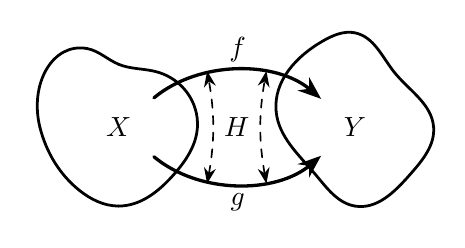
\begin{tikzpicture}[line width=1pt,line cap = round,>={Stealth[black]},every edge/.style={draw=black,very thick}]
        \node[fill=black,circle,inner sep=0pt,outer sep=0pt] at (0,0) (a) {};
        \node[fill=black,circle,inner sep=0pt,outer sep=0pt] at (-0.5,0.2) (b) {};
        \node[fill=black,circle,inner sep=0pt,outer sep=0pt] at (-1,1) (c) {};
        \node[fill=black,circle,inner sep=0pt,outer sep=0pt] at (-0.4,2) (d) {};
        \node[fill=black,circle,inner sep=0pt,outer sep=0pt] at (0, 1.8) (e) {};
        \node[fill=black,circle,inner sep=0pt,outer sep=0pt] at (0.5, 1.7) (f) {};
        \node[fill=black,circle,inner sep=0pt,outer sep=0pt] at (1,1) (g) {};
        \node[fill=black,circle,inner sep=0pt,outer sep=0pt] at (0.7,0.4) (h) {};
        \node at (0,1) (i) {$X$};
        \path[draw,use Hobby shortcut,closed=true](a) .. (b) .. (c) .. (d) .. (e) .. (f) .. (g) .. (h);
        \node[fill=black,circle,inner sep=0pt,outer sep=0pt] at (3,0) (a1) {};
        \node[fill=black,circle,inner sep=0pt,outer sep=0pt] at (2.5,0.4) (b1) {};
        \node[fill=black,circle,inner sep=0pt,outer sep=0pt] at (2,1.2) (c1) {};
        \node[fill=black,circle,inner sep=0pt,outer sep=0pt] at (2.6,2.1) (d1) {};
        \node[fill=black,circle,inner sep=0pt,outer sep=0pt] at (3, 2.2) (e1) {};
        \node[fill=black,circle,inner sep=0pt,outer sep=0pt] at (3.5, 1.7) (f1) {};
        \node[fill=black,circle,inner sep=0pt,outer sep=0pt] at (4,1) (g1) {};
        \node[fill=black,circle,inner sep=0pt,outer sep=0pt] at (3.7,0.4) (h1) {};
        \node at (3,1) (i1) {$Y$};
        \path[draw,use Hobby shortcut,closed=true](a1) .. (b1) .. (c1) .. (d1) .. (e1) .. (f1) .. (g1) .. (h1);
        \path[shorten >=0.2cm,shorten <=0.2cm,->] (i) edge[bend left=40] node[above] {$f$} (i1);
        \path[shorten >=0.2cm,shorten <=0.2cm,->] (i) edge[bend right=40] node[below] {$g$} (i1);
        \node at (1.5,1) (ho) {$H$};
        \node at (1.1,0.15) (t1) {};
        \node at (1.1,1.85) (t2) {};
        \node at (1.9,0.15) (t3) {};
        \node at (1.9,1.85) (t4) {};
        \path[draw=black,dashed,<->] (t1) edge[bend right =10,semithick] (t2);
        \path[draw=black,dashed,<->] (t3) edge[bend left =10,semithick] (t4);
    \end{tikzpicture}
    \caption[Surgery Theory - Homotopy Diagram]{Diagram for a homotopy between two functions $f,g:X\rightarrow Y$. $H$ `bends' $f$ into $g$, and vice-versa.}
    \label{fig:surgery_theory_course_homotopy_diagram_for_depicting_what_a_homotopy_is}
\end{wrapfigure}
Let $X$ and $Y$ be topological spaces, and let $f:X\rightarrow Y$ and $g:X\rightarrow Y$ be continuous functions. We now define what it means for $f$ and $g$ to be \textit{homotopic}.
\begin{definition}
A homotopy between continuous functions $f,g:X\rightarrow Y$ is a continuous function $H:X\times I \rightarrow Y$ such that $H(x,0)=f(x)$ and $H(x,1) = g(x)$.
\end{definition}
\begin{definition}
Homotopic functions are continuous functions $f,g:X\rightarrow Y$ with a homotopy between them.
\end{definition}
\begin{notation}
Homotopic functions $f,g:X\rightarrow Y$ are denoted $f\simeq g$.
\end{notation}
\begin{notation}
The set of continuous functions $f:X\rightarrow Y$ is denoted $C(X,Y)$.
\end{notation}
Figure \ref{fig:surgery_theory_course_homotopy_diagram_for_depicting_what_a_homotopy_is} shows two topological spaces and two continuous functions $f,g:X\rightarrow Y$. The homotopy $H$ `bends' $f$ into $g$, and vice-versa.
\begin{example}
Let $X = \mathbb{R}^{n}$ and $Y = \mathbb{R}^{m}$, where $n,m\in \mathbb{N}$. Let $f,g:\mathbb{R}^{n}\rightarrow \mathbb{R}^{m}$ be arbitrary continuous functions. The `straight line' homotopy is a homotopy between any such functions. Let $H:\mathbb{R}^{n}\times I \rightarrow \mathbb{R}^{m}$ be defined by $H(x,t) = (1-t)f(x)+tg(x)$. Then $H(x,0) = f(x)$, and $H(x,1) = g(x)$. Moreover, $H$ is continuous. So $H$ is a homotopy between $f$ and $g$, and $f$ and $g$ are homotopic. Note that $g(x) = constant$ is possible. Any continuous function $f:\mathbb{R}^{n}\rightarrow\mathbb{R}^{m}$ is homotopic to a point.
\end{example}
\begin{wrapfigure}[8]{r}{0.35\textwidth}
    \centering
    \vspace{-4ex}
    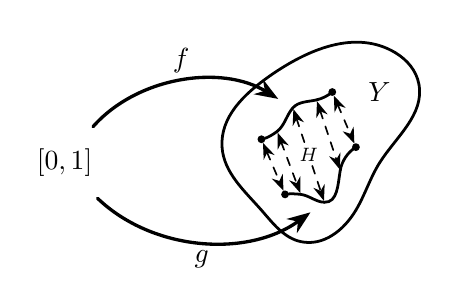
\begin{tikzpicture}[line width=1pt,line cap = round,>={Stealth[black]},every edge/.style={draw=black,very thick}]
        \node[fill=black,circle,inner sep=1pt,outer sep=0pt] at (2.5,1.3) (a0) {};
        \node[fill=black,circle,inner sep=0pt,outer sep=0pt] at (2.7,1.4) (b0) {};
        \node[fill=black,circle,inner sep=0pt,outer sep=0pt] at (2.9,1.7) (c0) {};
        \node[fill=black,circle,inner sep=0pt,outer sep=0pt] at (3.2,1.8) (d0) {};
        \node[fill=black,circle,inner sep=1pt,outer sep=0pt] at (3.4,1.9) (e0) {};
        \draw (a0) to [quick curve through={(b0) .. (c0) .. (d0)}] (e0);
        \node[fill=black,circle,inner sep=1pt,outer sep=0pt] at (2.8,0.6) (a1) {};
        \node[fill=black,circle,inner sep=0pt,outer sep=0pt] at (3,0.6) (b1) {};
        \node[fill=black,circle,inner sep=0pt,outer sep=0pt] at (3.3,0.5) (c1) {};
        \node[fill=black,circle,inner sep=0pt,outer sep=0pt] at (3.5,0.9) (d1) {};
        \node[fill=black,circle,inner sep=1pt,outer sep=0pt] at (3.7,1.2) (e1) {};
        \draw (a1) to [quick curve through={(b1) .. (c1) .. (d1)}] (e1);
        \path[draw=black,dashed,<->] (a0) edge[semithick] (a1);
        \path[draw=black,dashed,<->] (b0) edge[semithick] (b1);
        \path[draw=black,dashed,<->] (c0) edge[semithick] node[inner sep=0pt,outer sep=0pt,fill=white] {\scriptsize{\textit{H}}} (c1);
        \path[draw=black,dashed,<->] (d0) edge[semithick] (d1);
        \path[draw=black,dashed,<->] (e0) edge[semithick] (e1);
        \node[fill=black,circle,inner sep=0pt,outer sep=0pt] at (3,0) (a2) {};
        \node[fill=black,circle,inner sep=0pt,outer sep=0pt] at (2.5,0.4) (b2) {};
        \node[fill=black,circle,inner sep=0pt,outer sep=0pt] at (2,1.2) (c2) {};
        \node[fill=black,circle,inner sep=0pt,outer sep=0pt] at (2.6,2.1) (d2) {};
        \node[fill=black,circle,inner sep=0pt,outer sep=0pt] at (4.2, 2.4) (e2) {};
        \node[fill=black,circle,inner sep=0pt,outer sep=0pt] at (4.5, 2) (f2) {};
        \node[fill=black,circle,inner sep=0pt,outer sep=0pt] at (4,1) (g2) {};
        \node[fill=black,circle,inner sep=0pt,outer sep=0pt] at (3.7,0.4) (h2) {};
        \node at (0,1) (i) {$[0,1]$};
        \node at (4,1.9) (i1) {$Y$};
        \path[draw,use Hobby shortcut,closed=true](a2) .. (b2) .. (c2) .. (d2) .. (e2) .. (f2) .. (g2) .. (h2);
        \path[shorten >=0.2cm,shorten <=0.2cm,->] (i) edge[bend left=40] node[above] {$f$} (c0);
        \path[shorten >=0.2cm,shorten <=0.2cm,->] (i) edge[bend right=40] node[below] {$g$} (c1);
    \end{tikzpicture}
    \caption[Surgery Theory - Homotopy Diagram]{Diagram for a homotopy between two functions $f,g:[0,1]\rightarrow Y$. $H$ is the straight-line homotopy.}
    \label{fig:surgery_theory_course_homotopy_diagram_for_straight_line_homotopy}
\end{wrapfigure}
One can visualize a homotopy by letting $X = [0,1]$, and $Y\subset \mathbb{R}^{2}$ be a nice blob, like the one shown in Fig.~\ref{fig:surgery_theory_course_homotopy_diagram_for_straight_line_homotopy}. Let $f:[0,1]\rightarrow Y$ and $g:[0,1]\rightarrow Y$ be smooth curves within the blob. $H(x,t) = (1-t)f(x)+tg(x)$ is the map that drags $f(x)$ to $g(x)$ via the straight line connecting the two points. This is done for every point $x\in [0,1]$. The next thing to show is that the notion of homotopy $\simeq$ is an equivalence relation on the set of continuous functions from $X$ to $Y$, $C(X,Y)$.
\begin{theorem}
Homotopic is an equivalence relation on $C(X,Y)$.
\end{theorem}
\begin{proof}
We must show that $\simeq$ is reflexive, symmetric, and transitive.
\begin{enumerate}
    \item $\simeq$ is reflexive. Indeed, if $f\in C(X,Y)$, then let $H(x,t) = f(x)$. Then $H:X\times I \rightarrow Y$ is a continuous function, $H(x,0) = f(x)$, and $H(x,1) = f(x)$. Therefore, $H$ is a homotopy between $f$ and itself. That is, $f\simeq f$.
    \item $\simeq$ is symmetric. For if $f,g\in C(X,Y)$ and $f\simeq$, then there exists an $H:X\times I \rightarrow Y$ such that $H(x,0) = f(x)$ and $H(x,1) = g(x)$. Let $G(x,t) = F(x,1-t)$. But $(x,t)\mapsto (x,1-t)$ is a continuous mapping, and the composition of continuous functions is continuous, and therefore $G(x,t)$ is continuous. Moreover, $G(x,0) = H(x,1) = g(x)$, and $F(x,1) = G(x,0) = f(x)$. Therefore, $g\simeq f$.
    \item $\simeq$ is transitive. For if $f,g,h\in C(X,Y)$, $f\simeq g$, and $g\simeq h$, then there exists $H_{1}(x,t)$ such that $H_{1}(x,0) = f(x)$ and $H_{1}(x,1) = g(x)$, and there exists $H_{2}(x,t)$ such that $H_{2}(x,0) = g(x)$ and $H_{2}(x,1) = h(x)$. Let $H:X\times I\rightarrow Y$ be defined by
    \begin{equation*}
        H_{3}(x,t) = \begin{cases} H_{1}(x,2t), & 0\leq t\leq \frac{1}{2}\\ H_{2}(x,2t-1), & \frac{1}{2}<t\leq 1 \end{cases}
    \end{equation*}
    Then, by the pasting lemma, $H_{3}(x,t)$ is continuous. But $H_{3}(x,0) = H_{1}(x,0) = f(x)$, and $H_{3}(x,1) = H_{2}(x,1) = h(x)$. Therefore, $f\simeq h$.
\end{enumerate}
\end{proof}
\begin{definition}
Homotopy equivalent spaces are topological spaces $X,Y$ such that there exists functions $f\in C(X,Y)$ and $g\in C(Y,X)$ such that $f\circ g \simeq id_{Y}$, and $g\circ f \simeq id_{X}$.
\end{definition}
\begin{definition}
A homeomorphism from a topological space $X$ to a topological space $Y$ is a continuous bijection $f:X\rightarrow Y$ such that $f^{-1}:Y\rightarrow X$ is continuous.
\end{definition}
\begin{definition}
Homeomorphic topological spaces are spaces $X$ and $Y$ such that there exists a homeomorphism $f:X\rightarrow Y$ between them.
\end{definition}
\begin{theorem}
\label{theorem:surgery_theory_homeomorphic_implies_homotopy_equivalent}
If $X$ and $Y$ are homeomorphic, then they are homotopy equivalent.
\end{theorem}
\begin{proof}
If $X$ and $Y$ are homeomorphic, then there is a homeomorphism $f:X\rightarrow Y$. But then $f$ is a continuous map from $X$ to $Y$, and $f^{-1}$ is a continuous map from $Y$ to $X$. Moreover, $f\circ f^{-1} = id_{Y}$, and $f^{-1}\circ f = id_{X}$, for $f$ is a bijection. But $id_{X}\simeq id_{X}$, and $id_{Y}\simeq id_{Y}$. Therefore $X$ and $Y$ are homotopy equivalent.
\end{proof}
The study of surgery theory ask about the converse of theorem \ref{theorem:surgery_theory_homeomorphic_implies_homotopy_equivalent}. The converse of this theorem is not always true, as we will now demonstrate.
\begin{theorem}
\label{theorem:surgery_theory_homotopic_does_not_imply_homeomorphic}
There exist homotopy equivalent spaces that are not homeomorphic.
\end{theorem}
\begin{proof}
For let $X=\mathbb{R}^{2}$, and $Y = \{(0,0)\}$. Let $f:X\rightarrow Y$ be defined by $f(x,y) = (0,0)$. Let $g:Y\rightarrow X$ be defined by $g(x,y) = (x,y)$. Let $H_1(x,y,t) = (1-t)(x,y)$. Then $H_{1}$ is continuous, $H_{1}(x,y,0) = (x,y)$, and $H_{1}(x,y,0) = (0,0)$. Thus, $H_{1}$ is a homotopy between $g\circ f$ and $id_{X}$, and therefore $g\circ f \simeq id_{X}$. But also $f\circ g = id_{Y}$, and $id_{Y}\simeq id_{Y}$. Therefore $X$ and $Y$ are homotopy equivalent. But there is no homeomorphism from $X$ to $Y$. For suppose not. If $h:X\rightarrow Y$ is a homeomorphism, then it is a bijection. But if $h$ is a bijection, then $|X| = |Y|$. But $\mathbb{R}^2$ is uncountable, and $|Y| = 1$. A contradiction. Thus, $X$ and $Y$ are not homeomorphic.
\end{proof}
\begin{wrapfigure}[6]{r}{0.35\textwidth}
    \centering
    \vspace{-5ex}
    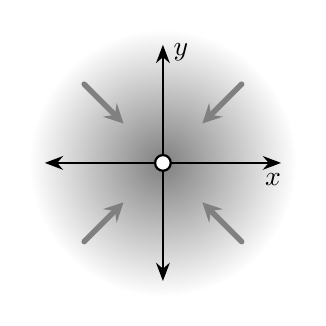
\begin{tikzpicture}[line width=1pt,line cap = round,>={Stealth[black]},every edge/.style={draw=black,very thick}]
        \filldraw[even odd rule,inner color=gray,outer color=white,draw=white] (0,0) circle (1.7);
        \draw[thick, <->] (-1.5,0) -- (1.5,0);
        \draw[thick, <->] (0,-1.5) -- (0,1.5);
        \draw[>=stealth,fill=gray,draw=gray,line width = 0.7mm,->](1,1) --++ (-0.5,-0.5);
        \draw[>=stealth,fill=gray,draw=gray,line width = 0.7mm,->](-1,-1) --++ (0.5,0.5);
        \draw[>=stealth,fill=gray,draw=gray,line width = 0.7mm,->](1,-1) --++ (-0.5,0.5);
        \draw[>=stealth,fill=gray,draw=gray,line width = 0.7mm,->](-1,1) --++ (0.5,-0.5);
        \node[fill=white,circle,thick, draw,inner sep=2pt,outer sep=3pt] at (0,0) (O) {};
        \node at (1.4,0) [below] {$x$};
        \node at (0,1.4) [right] {$y$};
    \end{tikzpicture}
    \vspace{-1ex}
    \caption{Retraction of $\mathbb{R}^{2}$ to $(0,0)$}
    \label{fig:surgery_theory_course_homotopy_equivalence_diagram_of_plane_with_point}
\end{wrapfigure}
Fig.~\ref{fig:surgery_theory_course_homotopy_equivalence_diagram_of_plane_with_point} shows the mapping $f$ between $\mathbb{R}^{2}$ and $\{(0,0)\}$. Theorem \ref{theorem:surgery_theory_homotopic_does_not_imply_homeomorphic} relies on the fact that $\mathbb{R}^2$ and $\{(0,0)\}$ are of different \textit{cardinality}. However, even if the topological spaces $X$ and $Y$ are homotopy equivalent, and are of the same cardinality, it is still possible that they are not homeomorphic.
\begin{theorem}
\label{theorem:surgery_theory_Homotopy_equivalance_of_plane_without_point_and_unit_disc_but_not_homeomorphic}
$\mathbb{R}^{2}\setminus\{(0,0)\}$ is homotopy equivalent to $S^{1}$, but not homeomorphic.
\end{theorem}
\begin{proof}
For let $X = \mathbb{R}^{2}\setminus\{(0,0)\}$, and let $Y = S^{1} = \{(x,y)\in \mathbb{R}^{2}:x^2+y^2=1\}$. Let $f:X\rightarrow Y$ be defined by $f(x,y) = \frac{(x,y)}{\norm{(x,y)}}$. Let $g:Y\rightarrow X$ be defined by $g(x,y) = (x,y)$. Let $H_1(x,y,t) = (1-t)\frac{(x,y)}{\norm{(x,y)}}+t(x,y)$. But then $H_1(x,y,0) = \frac{(x,y)}{\norm{x,y}}$, and $H_1(x,y,1) = (x,y)$. Thus $H_1$ is a homotopy between $g\circ f$ and $id_{X}$. But also $(f\circ g)(x,y) = (x,y)$, for all $(x,y)\in S^{1}$. Therefore $f\circ g= id_{Y}$, and $id_{Y}\simeq id_{Y}$. Therefore, $X$ and $Y$ are homotopy equivalent. However, $\dim(X) = 2$ and $\dim(Y) = 1$. But homeomorphisms preserve dimension. Therefore, $X$ and $Y$ are not homeomorphic.
\end{proof}
\begin{figure}[H]
    \centering
    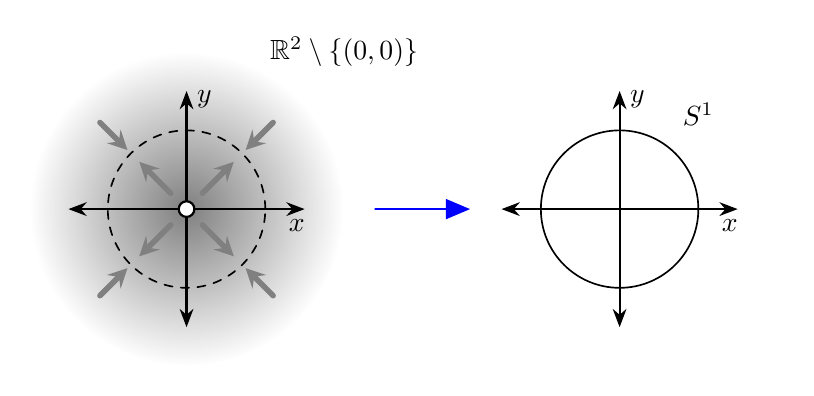
\begin{tikzpicture}[line width=1pt,line cap = round,>={Stealth[black]},every edge/.style={draw=black,very thick}]
        \filldraw[even odd rule,inner color=gray,outer color=white,draw=white] (0,0) circle (2);
        \draw[thick, <->] (-1.5,0) -- (1.5,0);
        \draw[thick, <->] (0,-1.5) -- (0,1.5);
        \draw[>=stealth,fill=gray,draw=gray,line width = 0.7mm,->](1.1,1.1) --++ (-0.35,-0.35);
        \draw[>=stealth,fill=gray,draw=gray,line width = 0.7mm,->](-1.1,-1.1) --++ (0.35,0.35);
        \draw[>=stealth,fill=gray,draw=gray,line width = 0.7mm,->](1.1,-1.1) --++ (-0.35,0.35);
        \draw[>=stealth,fill=gray,draw=gray,line width = 0.7mm,->](-1.1,1.1) --++ (0.35,-0.35);
        \draw[>=stealth,fill=gray,draw=gray,line width = 0.7mm,->](0.2,0.2) --++ (0.4,0.4);
        \draw[>=stealth,fill=gray,draw=gray,line width = 0.7mm,->](-0.2,-0.2) --++ (-0.4,-0.4);
        \draw[>=stealth,fill=gray,draw=gray,line width = 0.7mm,->](0.2,-0.2) --++ (0.4,-0.4);
        \draw[>=stealth,fill=gray,draw=gray,line width = 0.7mm,->](-0.2,0.2) --++ (-0.4,0.4);
        \draw[dashed,draw=black,semithick] (0,0) circle (1);
        \node[fill=white,circle,thick, draw,inner sep=2pt,outer sep=3pt] at (0,0) (O) {};
        \node at (1.4,0) [below] {$x$};
        \node at (0,1.4) [right] {$y$};
        \node at (2,2) {$\mathbb{R}^{2}\setminus \{(0,0)\}$};
        \draw[>=triangle 45,draw=blue,->](2.4,0) --++ (1.2,0);
        \draw[thick, <->] (4,0) -- (7,0);
        \draw[thick, <->] (5.5,-1.5) -- (5.5,1.5);
        \draw[draw=black,semithick] (5.5,0) circle (1);
        \node at (6.9,0) [below] {$x$};
        \node at (5.5,1.4) [right] {$y$};
        \node at (6.5,1.2) {$S^{1}$};
        \node at (7.5,0) {};
    \end{tikzpicture}
    \caption[Surgery Theory - HE From $\mathbb{R}^2\setminus\{(0,0)\}$ to $S^{1}$]{Homotopy Equivalence of $\mathbb{R}^{2}\setminus\{(0,0)\}$ and $S^{1}$}
    \label{fig:surgery_theory_homotopy_equivalence_between_the_plane_with_a_point_removed_and_the_unit_circle}
\end{figure}
Theorem \ref{theorem:surgery_theory_Homotopy_equivalance_of_plane_without_point_and_unit_disc_but_not_homeomorphic} relies on the fact that $\mathbb{R}^{2}\setminus \{(0,0)\}$ and $S^{1}$ are of different \textit{dimension}. However, even if $X$ and $Y$ are of the same cardinality \textit{and} of the same dimension, it is still possible that they are homotopy equivalent, but not homeomorphic. First, we show that $S^{2}\setminus \{(0,0,1)\}$ is homeomorphic to $D^{2}$.
\begin{theorem}
\label{theorem:surgery_theory_the_sphere_with_a_point_removed_is_homeomorphic_to_the_plane}
$S^{3}\setminus \{(0,0,1)\}$ is homeomorphic to $\mathbb{R}^{2}$
\end{theorem}
\begin{proof}
For let $f:S^{3}\setminus \{(0,0,1)\}\rightarrow \mathbb{R}^{2}$ be the stereographic projection mapping. That is, $f(x,y,z) = (\frac{x}{1-z},\frac{y}{1-z})$, for $(x,y,z)\in S^{2}\setminus \{(0,0,1)\}$. If $(X,Y) \in \mathbb{R}^{2}$, let:
\begin{equation*}
     x = \frac{2X}{\norm{(X,Y)}^{2}+1} \quad\quad y = \frac{2Y}{\norm{(X,Y)}^{2}+1}   \quad\quad z = \frac{\norm{(X,Y)}^{2}-1}{\norm{(X,Y)}^{2}+1} 
\end{equation*}
Then:
\begin{equation*}
    \bigg(\frac{x}{1-z},\frac{y}{1-z}\bigg) = \bigg(\frac{\frac{2X}{\norm{(X,Y)}^{2} + 1}}{\frac{2}{\norm{(X,Y)}^{2}+1}},\frac{\frac{2Y}{\norm{(X,Y)}^{2}+1}}{\frac{2}{\norm{(X,Y)}^{2}+1}}\bigg) = (X,Y)    
\end{equation*}
and
\begin{align*}
    \norm{(x,y,z)} &= \sqrt{\frac{4X^{2}}{\big(\norm{(X,Y)}^{2}+1\big)^{2}} + \frac{4Y^{2}}{\big(\norm{(X,Y)}^{2}+1\big)^{2}} + \frac{(\norm{(X,Y)}^{2}-1)^{2}}{(\norm{(X,Y)}^{2}+1)^{2}}}\\
    &= \sqrt{\frac{4\norm{(X,Y)}^{2} + \norm{(X,Y)}^{4} - 2\norm{(X,Y)}^{2} + 1}{(\norm{(X,Y)}+1)^{2}}}\\
    &= \sqrt{\frac{\norm{(X,Y)}^{4} + 2\norm{(X,Y)}^{2} + 1}{(\norm{(X,Y)}^{2}+1)^{2}}}\\
    &= \sqrt{\frac{(\norm{(X,Y)}^{2}+1)^{2}}{(\norm{(X,Y)}^{2}+1)^{2}}}\\
    &= 1
\end{align*}
Thus, $(x,y,z) \in S^{2}\setminus \{(0,0,1)\}$, and $f$ is surjective. If $f(x_1,y_1,z_1) = f(x_2,y_2,z_2)$, then $z_{1} = z_{2}$. For as $(x_1,y_1,z_1)\in S^{2}\setminus\{(0,0,1)\}$, and therefore $x_{1}^{2} + y_{1}^{2} = 1-z_{1}^{2}$, we have:
\begin{equation*}
    \norm{(X,Y)}^{2} = \frac{x_{1}^2+y_{1}^2}{(1-z_{1})^{2}} = \frac{1-z_{1}^{2}}{(1-z_{1})^{2}}
\end{equation*}
%
But:
%
\begin{equation*}
    \norm{(X,Y)}^{2} = \frac{x_{2}^{2}+y_{2}^{2}}{(1-z_{2})^{2}} = \frac{1-z_{2}^{2}}{(1-z_{2})^{2}}   
\end{equation*}
%
So we have $\frac{1-z_{1}^{2}}{(1-z_{1})^{2}} = \frac{1-z_{2}^{2}}{(1-z_{2})^{2}}$. Simplifying, we get:
\begin{equation*}
    \frac{1+z_{1}}{1-z_{1}} = \frac{1+z_{2}}{1-z_{2}}   
\end{equation*}
%
But $f(x) = \frac{1+x}{1-x}$ is an injective function, and therefore $z_{1} = z_{2}$. From this:
%
\begin{equation*}
    \frac{x_{1}}{1-z_{1}} = \frac{x_{2}}{1-z_{2}} \Rightarrow x_{1} = x_{2}
\end{equation*}
%
Similarly, $y_{1} = y_{2}$. Thus, $f$ is injective. So $f$ is a bijection. Moreoever, $f$ is continuous as $\frac{x}{1-z}$ and $\frac{y}{1-z}$ are continuous. Finally:
\begin{equation*}
    f^{-1}(X,Y) = \bigg(\frac{2X}{\norm{(X,Y)}^{2}+1},\frac{2Y}{\norm{(X,Y)}^{2}+1},\frac{\norm{(X,Y)}^{2}-1}{\norm{(X,Y)}^{2}+1}\bigg)
\end{equation*}
Which is continuous. $f$ is a homeomorphism.
\end{proof}
Fig.~\ref{fig:surgery_theory_stereographic_projection_of_sphere_to_plane_homeomorphism} depicts the stereographic projection used to prove theorem \ref{theorem:surgery_theory_the_sphere_with_a_point_removed_is_homeomorphic_to_the_plane}. It can be seen that $(0,0,1)$ projects `to infinite'. Because of this, it is not uncommon to call this point infinity. Next, we prove that $\mathbb{R}^{2}$ is homeomorphic to $D^{2}$, almost completing our claim that $S^{2}\setminus \{(0,0,1)\}$ is homeomorphic to $D^{2}$.
\begin{theorem}
$\mathbb{R}^{2}$ is homeomorphic to $D^{2}$.
\end{theorem}
\begin{proof}
Let $f:D^{2}\rightarrow \mathbb{R}^{2}$ be defined by $f(\mathbf{x}) = \frac{\mathbf{x}}{1-\norm{\mathbf{x}}}$. $f$ is surjective. For $\mathbf{0}\mapsto \mathbf{0}$. If $\mathbf{y}\in \mathbb{R}^2\setminus \mathbf{0}$, then let $\mathbf{x} = \frac{\mathbf{y}}{1+\norm{\mathbf{y}}}$. Then $\norm{\mathbf{x}} = \frac{\norm{\mathbf{y}}}{1+\norm{\mathbf{y}}} < 1$, and thus $\mathbf{x}\in D^{2}$. But $f(\mathbf{x}) = \frac{\frac{\mathbf{y}}{1+\norm{\mathbf{y}}}}{1 - \frac{\norm{\mathbf{y}}}{1+\norm{\mathbf{y}}}} = \mathbf{y}$. $f$ is surjective. Moreover, $f$ is injective. For if $f(\mathbf{x}_{1}) = f(\mathbf{x}_{2})$, then $\frac{\norm{\mathbf{x}_{1}}}{1+\norm{\mathbf{x}_{1}}} = \norm{f(\mathbf{x}_{1})} = \norm{f(\mathbf{x}_{2})} = \frac{\norm{\mathbf{x}_{2}}}{1+\norm{\mathbf{x}}_{2}}$, and therefore $\norm{\mathbf{x}}_{1} = \norm{\mathbf{x}_{2}}$. But $\frac{\mathbf{x}_{1}}{1+\norm{\mathbf{x}_{1}}} = \frac{\mathbf{x}_{2}}{1+\norm{\mathbf{x}_{2}}}$, and therefore $\mathbf{x}_{1} = \mathbf{x}_{2}$. $f$ is bijective. Moreover, $f$ is continuous. Finally, $f^{-1}(\mathbf{y}) = \frac{\mathbf{y}}{1+\norm{\mathbf{y}}}$ is continuous. $f$ is a homeomorphism.
\end{proof}
\begin{figure}[t]
    \centering
    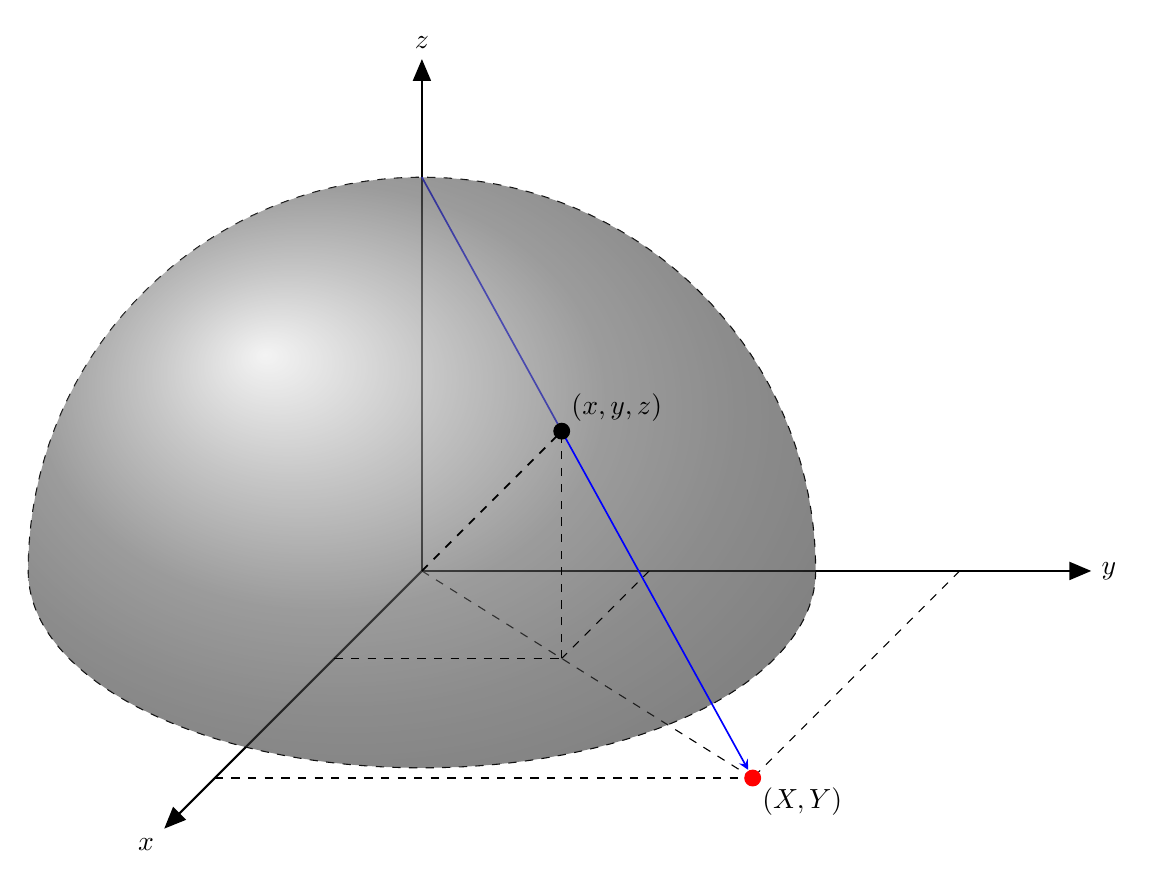
\begin{tikzpicture}[scale=5,>=triangle 45]
        %draw the main coordinate system axes
        \draw[thick,->] (0,0,0) -- (1.7,0,0) node[right]{$y$};
        \draw[thick,->] (0,0,0) -- (0,1.3,0) node[above]{$z$};
        \draw[thick,->] (0,0,0) -- (0,0,1.7) node[below left]{$x$};
        %draw some dashed arcs, demonstrating direct arc drawing
        \draw[dashed] (1cm,0) arc (0:-180:1cm and 5mm) arc (180:0:1cm and 1cm);
        \coordinate (A) at (0.57735026918962,0.57735026918962,0.57735026918962);
        \node[circle,inner sep=0pt, outer sep=1mm] (B) at (1.3660254037844,0,1.3660254037844) {};
        \draw[draw=blue,semithick] (0,1,0) -- (A);
        \draw[dashed] (0,0,0) -- (1.3660254037844,0,1.3660254037844);
        \shade[ball color=gray,opacity=0.6] (1cm,0) arc (0:-180:1cm and 5mm) arc (180:0:1cm and 1cm);
        \draw[draw=blue,semithick,>=stealth,->] (A) -- (B);
        \draw[dashed,thin] (0,0,1.3660254037844) -- (1.3660254037844,0,1.3660254037844);
        \draw[dashed,thin] (1.3660254037844,0,0) -- (1.3660254037844,0,1.3660254037844);
        \draw[dashed,semithick] (0,0,0) -- (0.57735026918962,0.57735026918962,0.57735026918962);
        \draw[dashed,thin]      (0,0,0.57735026918962) -- (0.57735026918962,0,0.57735026918962);
        \draw[dashed,thin]      (0.57735026918962,0,0) -- (0.57735026918962,0,0.57735026918962);
        \draw[dashed,thin]      (0.57735026918962,0,0.57735026918962) -- (0.57735026918962,0.57735026918962,0.57735026918962);
        \draw[dashed,thin]      (0,0,0.57735026918962) -- (0.57735026918962,0,0.57735026918962);
        \filldraw[black] (0.57735026918962,0.57735026918962,0.57735026918962) circle (0.2mm);
        \filldraw[red]   (1.3660254037844,0,1.3660254037844) circle (0.2mm);
        \node at (A) [above right] {$(x,y,z)$};
        \node at (B) [below right] {$(X,Y)$};
    \end{tikzpicture}
    \caption[Surgery Theory - Stereographic Projection]{Stereographic Projection of the Sphere onto the Plane}
    \label{fig:surgery_theory_stereographic_projection_of_sphere_to_plane_homeomorphism}
\end{figure}
\begin{theorem}
$S^{2}\setminus\{(0,0,1)\}$ is homeomorphic to $D^{2}$.
\end{theorem}
\begin{proof}
For $S^{2}\setminus\{(0,0,1)\}$ is homeomorphic to $\mathbb{R}^{2}$, and $\mathbb{R}^{2}$ is homeomorphic to $D^{2}$. But homeomorphism is an equivalence relation, so $S^{2}\setminus\{(0,0,1)\}$ is homeomorphic to $D^{2}$.
\end{proof}
\begin{figure}[H]
    \centering
    \resizebox{\textwidth}{!}{
    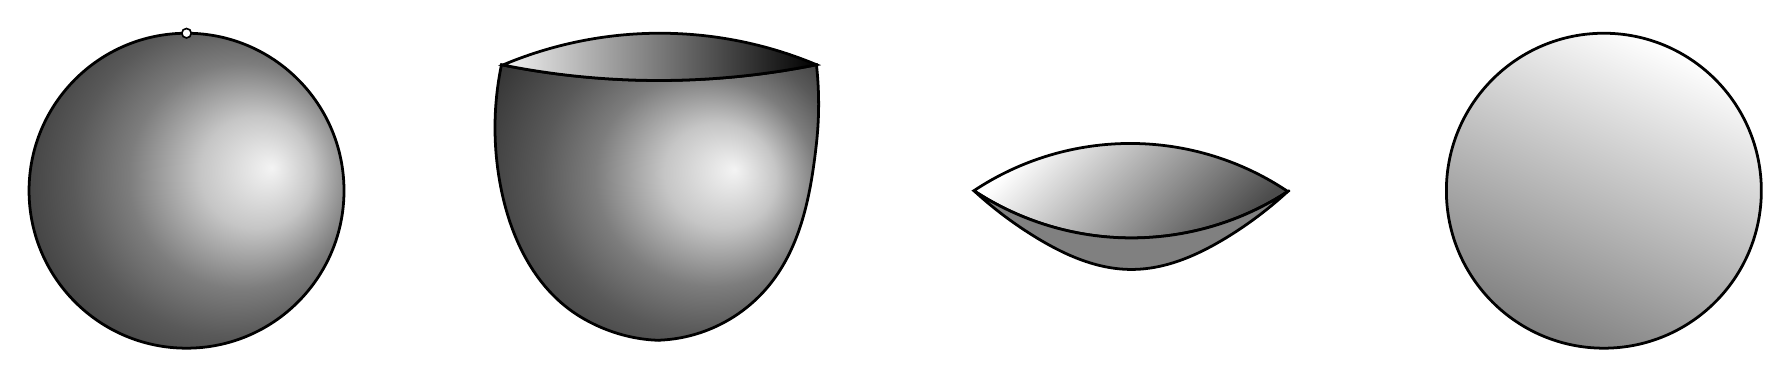
\begin{tikzpicture}[scale=2,line width=1pt,line cap = round,>={Stealth[black]},every edge/.style={draw=black,very thick}]
        \filldraw[ball color = gray!60!white,draw=black, shading angle = 240] (-4,0) circle (1);
        \filldraw[white,draw=black,semithick]   (-4,1) circle (0.3mm);
        \node[fill=black,circle,inner sep=0pt,outer sep=0pt] at (-1,-0.95) (a) {};
        \node[fill=black,circle,inner sep=0pt,outer sep=0pt] at (-1.5,-0.8) (b) {};
        \node[fill=black,circle,inner sep=0pt,outer sep=0pt] at (-2,0) (c) {};
        \node[fill=black,circle,inner sep=0pt,outer sep=0pt] at (-2,0.8) (d) {};
        \node[fill=black,circle,inner sep=0pt,outer sep=0pt] at (-1, 0.7) (e) {};
        \node[fill=black,circle,inner sep=0pt,outer sep=0pt] at (0, 0.8) (f) {};
        \node[fill=black,circle,inner sep=0pt,outer sep=0pt] at (-0,0.3) (g) {};
        \node[fill=black,circle,inner sep=0pt,outer sep=0pt] at (-0.3,-0.6) (h) {};
        \node[fill=black,circle,inner sep=0pt,outer sep=0pt] at (-1, 1) (top) {};
        \path[draw=black,ball color=gray!60!white, shading angle = 250 ] (a) to [quick curve through={(b) .. (c)}] (d) to [quick curve through={(e)}] (f) to [quick curve through={(g) .. (h)}] cycle;
        \path[draw=black,left color = white!90!gray, right color = black] (d) to [quick curve through={(e)}] (f) to [quick curve through={(top)}] cycle;
        \node[fill=black,circle,inner sep=0pt,outer sep=0pt] at (2,-0.5)     (a1) {};
        \node[fill=black,circle,inner sep=0pt,outer sep=0pt] at (1.4,-0.3) (b1) {};
        \node[fill=black,circle,inner sep=0pt,outer sep=0pt] at (1,0) (c1) {};
        \node[fill=black,circle,inner sep=0pt,outer sep=0pt] at (2,-0.3) (BOT1) {};
        \node[fill=black,circle,inner sep=0pt,outer sep=0pt] at (2,0.3) (TOP1) {};
        \node[fill=black,circle,inner sep=0pt,outer sep=0pt] at (3,0) (d1) {};
        \node[fill=black,circle,inner sep=0pt,outer sep=0pt] at (2.6,-0.3) (e1) {};
        \path[draw=black,left color=white, right color = white!30!black, shading angle = 45] (d1) to [quick curve through={(BOT1)}] (c1) to [quick curve through={(TOP1)}] cycle;
        \path[draw=black,fill=gray] (d1) to [quick curve through={(BOT1)}] (c1) to [curve through={(b1) (a1) (e1)}] cycle;
        \filldraw[draw=black,right color = white, left color = white!50!black,shading angle = 155] (5,0) circle (1);
    \end{tikzpicture}}
    \caption[Surgery Theory - Homeomorphism From $S^{2}\setminus\{(0,0,1)\}$ and $D^{2}$]{The unit sphere with a point removed can be continuously deformed into the open unit disc.}
    \label{fig:my_label}
\end{figure}
We can use the fact that $S^{2}\setminus \{(0,0,1)\}$ is homeomorphic to $D^{2}$ to construct examples of topological manifolds of the same dimensions that are homotopy equivalent, but not homeomorphic. We may generalize to $S^{2}$ with $n$ points removed is homeomorphic to $D^{2}$ with $n-1$ points removed. We now define the notion of \textit{manifold} and \textit{dimension}.
\begin{definition}
An $n$ dimensional manifold is a Hausdorff topological space $X$ such that for all $p\in X$ there is an open neighborhood $\mathcal{U}$ of $p$, such that $\mathcal{U}$ is homeomorphic to $\mathbb{R}^{n}$.
\end{definition}
It can be shown that if $X$ and $Y$ are homeomorphic manifolds, then they are of the same dimension. This is simply because $\mathbb{R}^{n}$ is homeomorphic to $\mathbb{R}^{m}$ if and only if $n=m$. Therefore, homeomorphism preserve dimension. We use the fact that a sphere is not homeomorphic to a torus. We also use the following visual representation of a torus:
\begin{figure}[H]
    \centering
    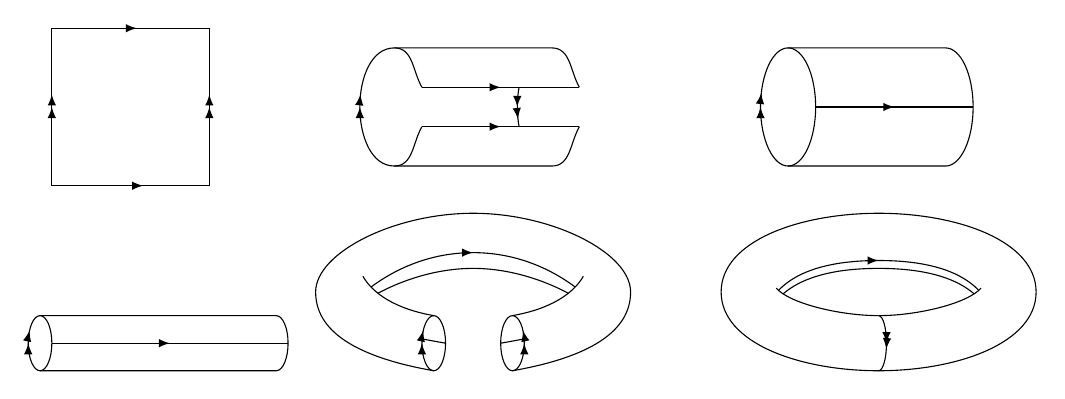
\begin{tikzpicture}
        \draw[postaction={decorate},decoration={
            markings,
            mark=at position .145 with {\arrow{latex}},
            mark=at position .375 with {\arrow{latex}},
            mark=at position .395 with {\arrow{latex}},
            mark=at position .615 with {\arrowreversed{latex}},
            mark=at position .855 with {\arrowreversed{latex}},
            mark=at position .875 with {\arrowreversed{latex}}}]
            (0,-1) -- +(2,0) -- +(2,2) -- +(0,2) -- cycle;
        \begin{scope}[xshift=4.7cm]
            \draw[postaction={decorate},decoration={
            markings,
            mark=at position .5 with {\arrow{latex}}}]
            (0,.25) -- ++(2,0);
            \draw[postaction={decorate},decoration={
            markings,
            mark=at position .5 with {\arrow{latex}}}]
            (0,-.25) -- ++(2,0);
            \draw[postaction={decorate},decoration={
            markings,
            mark=at position .5 with {\arrow{latex}},
            mark=at position .55 with {\arrow{latex}}}]
            (0,-.25) to[out=-120,in=0] (-.35,-.75) to[out=180,in=180] (-.35,.75) to[out=0,in=120] (0,.25);
            \draw (2,.25) to[out=120,in=0] (1.65,.75) -- (-.35,.75) (-.35,-.75) --  (1.65,-.75) to[out=0,in=-120] (2,-.25);
            \clip (0,.25) rectangle (2,-.25);
            \draw[postaction={decorate},decoration={
            markings,
            mark=at position .5 with {\arrow{latex}},
            mark=at position .58 with {\arrow{latex}}}]
            (1.65,.75) to[out=180,in=180] (1.65,-.75);
        \end{scope}
        \begin{scope}[xshift=9.7cm]
            \draw[postaction={decorate},decoration={
            markings,
            mark=at position .5 with {\arrow{latex}},}]
            (0,0) -- (2,0);
            \draw[postaction={decorate},decoration={
            markings,
            mark=at position .5 with {\arrow{latex}},
            mark=at position .55 with {\arrow{latex}}}]
            (0,0) arc[start angle=0,delta angle=-360,x radius=.35,y radius=.75];
            \draw (2,0) arc[start angle=0,delta angle=-90,x radius=.35,y radius=.75] -- ++(-2,0);
            \draw (2,0) arc[start angle=0,delta angle=90,x radius=.35,y radius=.75] -- ++(-2,0);
        \end{scope}
        \begin{scope}[yshift=-3cm]
            \draw[postaction={decorate},decoration={
            markings,
            mark=at position .5 with {\arrow{latex}},}]
            (0,0) -- (3,0);
            \draw[postaction={decorate},decoration={
            markings,
            mark=at position .5 with {\arrow{latex}},
            mark=at position .6 with {\arrow{latex}},}]
            (0,0) arc[start angle=0,delta angle=-360,x radius=.15,y radius=.35];
            \draw (3,0) arc[start angle=0,delta angle=-90,x radius=.15,y radius=.35] -- ++(-3,0);
            \draw (3,0) arc[start angle=0,delta angle=90,x radius=.15,y radius=.35] -- ++(-3,0);
        \end{scope}
        \begin{scope}[xshift=4cm,yshift=-3cm]
            \draw[postaction={decorate},decoration={
            markings,
            mark=at position .5 with {\arrow{latex}},
            mark=at position .6 with {\arrow{latex}},}]
            (1,0) arc[start angle=0,delta angle=-360,x radius=.15,y radius=.35];
            \draw (1,0) ++(-.15,-.35) .. controls +(170:1) and +(-90:.5) .. ++(-1.5,1) .. controls +(90:.5) and +(180:1) .. ++(2,1) .. controls +(0:1) and +(90:.5) .. ++(2,-1) .. controls +(-90:.5) and +(10:1) .. ++(-1.5,-1) coordinate (a);
            \draw[postaction={decorate},decoration={
            markings,
            mark=at position .5 with {\arrow{latex}},
            mark=at position .6 with {\arrow{latex}},}]
            (a) ++(-.15,.35) arc[start angle=0,delta angle=-360,x radius=-.15,y radius=.35];
            \draw (1,0) ++(-.15,.35) .. controls +(170:.5) and +(-60:.25) .. ++(-.9,.5) coordinate (b);
            \draw (a) ++(0,.7) .. controls +(10:.5) and +(240:.25) .. ++(.9,.5) coordinate (c);
        \end{scope}
        \begin{scope}[xshift=4cm,yshift=-3cm]
            \clip (1,0) ++(-.15,.35) .. controls +(170:.5) and +(-60:.25) .. ++(-.9,.5) -- ++(0,2) -| (c)  .. controls +(240:.25) and +(10:.5) .. ++(-.9,-.5);
            \draw (1,0) ++(-.15,-.35) ++(0,-.7) .. controls +(170:1) and +(-90:.5) .. ++(-1.5,.8) .. controls +(90:.5) and +(180:1) .. ++(2,1.2) .. controls +(0:1) and +(90:.5) .. ++(2,-1.2) .. controls +(-90:.5) and +(10:1) .. ++(-1.5,-.8);
            \draw[postaction={decorate},decoration={
            markings,
            mark=at position .5 with {\arrow{latex}},}]
            (1,0) ++(-.15,-.35) ++(0,-.8) .. controls +(170:1) and +(-90:.5) .. ++(-1.5,.8) .. controls +(90:.5) and +(180:1.2) .. ++(2,1.5) .. controls +(0:1.2) and +(90:.5) .. ++(2,-1.5) .. controls +(-90:.5) and +(10:1) .. ++(-1.5,-.8);
        \end{scope}
        \begin{scope}[xshift=4cm,yshift=-3cm]
        \clip  (a) ++(-.15,.35) arc[start angle=0,delta angle=-360,x radius=-.15,y radius=.35];
        \draw (a) ++(-.15,.35) .. controls +(10:1) and +(-90:.5) .. ++(1.5,.8);
        \end{scope}
        \begin{scope}[xshift=4cm,yshift=-3cm]
        \clip (1,0) arc[start angle=0,delta angle=-360,x radius=.15,y radius=.35];
        \draw (1,0) .. controls +(170:1) and +(-90:.5) .. ++(-1.5,.8);
        \end{scope}
        \begin{scope}[xshift=9cm,yshift=-3cm]
            \draw[postaction={decorate},decoration={
            markings,
            mark=at position .5 with {\arrow{latex}},
            mark=at position .6 with {\arrow{latex}},}]
            (1.5,.35) arc[start angle=90,end angle=-90,y radius=.35,x radius=.1];
            \draw (1.5,-.35) .. controls +(180:1) and +(-90:.65) .. ++(-2,1) .. controls +(90:.65) and +(180:1) .. ++(2,1) .. controls +(0:1) and +(90:.65) .. ++(2,-1) .. controls +(-90:.65) and +(0:1) .. ++(-2,-1); \draw (1.5,.35) .. controls +(180:.5) and +(-50:.25) .. ++(-1.3,.35) coordinate (b);
            \draw (1.5,.35) .. controls +(0:.5) and +(230:.25) .. ++(1.3,.35) coordinate (c);
        \end{scope}
        \begin{scope}[xshift=9cm,yshift=-3cm]
            \clip (1.5,.35) .. controls +(180:.5) and +(-50:.25) .. ++(-1.3,.35) -- ++(0,2) -| (c)  .. controls +(230:.25) and +(0:.5) .. ++(-1.3,-.35);
            \draw (1.5,-.35) ++(0,-.7) .. controls +(180:1) and +(-90:.65) .. ++(-1.5,1) .. controls +(90:.65) and +(180:1) .. ++(1.5,1) .. controls +(0:1) and +(90:.65) .. ++(1.5,-1) .. controls +(-90:.65) and +(0:1) .. ++(-1.5,-1);
            \draw[postaction={decorate},decoration={
            markings,
            mark=at position .5 with {\arrow{latex}},}]
            (1.5,-.35) ++(0,-.6) .. controls +(180:1) and +(-90:.65) .. ++(-1.5,1) .. controls +(90:.65) and +(180:1) .. ++(1.5,1) .. controls +(0:1) and +(90:.65) .. ++(1.5,-1) .. controls +(-90:.65) and +(0:1) .. ++(-1.5,-1);
        \end{scope}
    \end{tikzpicture}
    \caption[Surgery Theory - Plane Representation of a Torus]{The unit square with a particular equivalence relation on it can be used to represent a torus.}
    \label{fig:surgery_theory_plane_representation_of_a_torus}
\end{figure}
\begin{theorem}
There exist manifolds $X$ and $Y$ such that $\dim(X) = \dim(Y)$, $X\simeq Y$, yet $X$ and $Y$ are not homeomorphic.
\end{theorem}
\begin{proof}
For let $X = S^{2}\setminus\{(0,0,1),(0,1,0),(1,0,0)\}$, and let $Y = T^{2}\setminus\{(1,0,0)\}$. That is, $X$ is a sphere with three points removed, and $Y$ is a torus with one point removed. Then $\dim(X) = \dim(Y) = 2$. Moreover, $X\simeq Y$. For $X$ is homeomorphic to the plane with $2$ points removed. This is homotopy equivalent to a figure $8$. Using the square representation of a torus in Fig.~\ref{fig:surgery_theory_plane_representation_of_a_torus} we see that the torus with a point removed is also homotopy equivalent to a figure $8$. But homotopy equivalence is an equivalence relation, and thus $X\simeq Y$. But the a sphere is not homeomorphic to a torus, and similarly a sphere with $3$ points removed is not homeomorphic to a torus with $1$ point removed.
\end{proof}
Fig.~\ref{fig:surgery_theory_homotopy_equivalence_sphere_with_3_holes_torus_with_1_hole} shows how both $S^{2}$ with three points removed and $T^{2}$ with one point removed are homotopy equivalent. Recall that $\mathbb{R}^{2}\setminus \{(0,0)\}$ is homotopy equivalent to $S^{1}$. In a similar manner, the plane with two points removed is homotopy equivalent to two circles whose intersection contains a single points (That is, a figure-$8$). While the ``Proof," given was hand wavy, the fact that the sphere is not homeomorphic to the torus comes from the fact that these two objects have different boundary components, something preserved by homeomorphism. Intiutively, one can think of removing a great circle (Or a ``line") from the sphere. Removing such an object creates two disconnected components. However, removing a circle from the torus still leaves one connected surface. The next question is ``What about compact manifolds without boundary?"
\begin{theorem}[The Generalized Poincare-Conjecture]
If $X$ is an $n$ dimensional manifold that is homotopy equivalent to $S^{n+1}$, then $X$ is homeomorphic to $S^{n+1}$.
\end{theorem}
\begin{definition}
A rigid manifold is a manifold $X$ such that for all homotopy equivalent closed manifolds $Y$, $X$ is homeomorphic to $Y$.
\end{definition}
\begin{figure}[H]
    \centering
    \resizebox{!}{0.3\textheight}{
    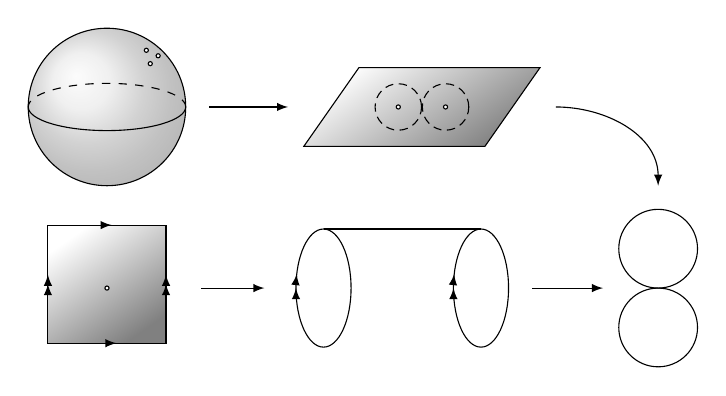
\begin{tikzpicture}
        \shade[ball color = gray!40, opacity = 0.4] (0,0) circle (1cm);
        \draw (0,0) circle (1cm);
        \draw (-1,0) arc (180:360:1 and 0.3);
        \draw[dashed] (1,0) arc (0:180:1 and 0.3);
        \fill[fill=white,draw=black] (0.55,0.55) circle (0.75pt);
        \fill[fill=white,draw=black] (0.65,0.65) circle (0.75pt);
        \fill[fill=white,draw=black] (0.5,0.72)  circle (0.75pt);
        \draw[>=latex,draw=black,->] (1.3cm,0) -- (2.3cm,0);
        \shade[fill = gray,shading angle = 215](2.5cm,-0.5cm) -- (3.2cm, 0.5cm) -- (5.5cm,0.5cm) -- (4.8cm,-0.5cm) -- cycle;
        \draw (2.5cm,-0.5cm) -- (3.2cm, 0.5cm) -- (5.5cm,0.5cm) -- (4.8cm,-0.5cm) -- cycle;
        \draw[draw=black,densely dashed] (3.7cm,0) circle (0.295cm);
        \draw[draw=black,densely dashed] (4.3cm,0) circle (0.295cm);
        \fill[fill=white,draw=black] (3.7cm,0) circle (0.75pt);
        \fill[fill=white,draw=black] (4.3cm,0) circle (0.75pt);
        \draw[>=latex,draw=black,->] (5.7cm,0) to [in=90, out=0] (7cm,-1cm);
        \draw[>=latex,draw=black,->] (1.2cm,-2.3cm) -- (2cm,-2.3cm);
        \shade[fill = gray,shading angle = 215](-0.75,-3cm) -- +(1.5cm,0) -- +(1.5cm,1.5cm) -- +(0,1.5cm) -- cycle;
        \fill[fill=white,draw=black] (0,-2.3cm) circle (0.75pt);
        \draw[postaction={decorate},decoration={
            markings,
            mark=at position .145 with {\arrow{latex}},
            mark=at position .375 with {\arrow{latex}},
            mark=at position .395 with {\arrow{latex}},
            mark=at position .615 with {\arrowreversed{latex}},
            mark=at position .855 with {\arrowreversed{latex}},
            mark=at position .875 with {\arrowreversed{latex}}}]
        (-0.75,-3cm) -- +(1.5cm,0) -- +(1.5cm,1.5cm) -- +(0,1.5cm) -- cycle;
        \draw[postaction={decorate},decoration={
            markings,
            mark=at position .5 with {\arrow{latex}},
            mark=at position .55 with {\arrow{latex}}}]
            (3.1cm,-2.3cm) arc[start angle=0,delta angle=-360,x radius=.35,y radius=.75];
            \draw (2.75cm,-1.55cm) -- ++(2cm,0);
            \draw[postaction={decorate},decoration={
            markings,
            mark=at position .5 with {\arrow{latex}},
            mark=at position .55 with {\arrow{latex}}}]
            (5.1cm,-2.3cm) arc[start angle=0,delta angle=-360,x radius=.35,y radius=.75];
        \draw[>=latex,draw=black,->] (5.4cm,-2.3cm) -- (6.3cm,-2.3cm);
        \draw[draw = black] (7cm,-1.8cm) circle (0.5cm);
        \draw[draw = black] (7cm,-2.8cm) circle (0.5cm);
    \end{tikzpicture}}
    \caption{Caption}
    \label{fig:surgery_theory_homotopy_equivalence_sphere_with_3_holes_torus_with_1_hole}
\end{figure}
The question then becomes ``Which manifolds are rigid, and which are not?" From the Poincare theorem, $S^{n}$ is rigid for all $n\in \mathbb{N}$. The first example of a non-rigid manifold came in the 1930's from Franz, Reidemeister, and de Rham, and is called a Lens Space. Let $p$ and $q$ be coprime positive integers. Divide $S^{3}$ into $p$ equal parts, and then divide this into its northern and southern hemispheres. Take a piece of the northern hemisphere and move it over $q$ pieces, and then glue this to the southern hemisphere. Take the piece that is already there and move it over $q$ pieces, and then glue that to the northern hemisphere. Repeat this process until all slices are done. The is called the Lens Space $L(p,q)$. $L(1,1)$ is simply the sphere. $L(2,1)$ is the real projective plane $\mathbb{RP}^{2}$. See Fig.~\ref{fig:surgery_theory_lens_space_drawing} to see how this construction occurs. It can be shown that for distinct pairs $(p,q), (p',q')$, that $L(p,q)$ is homotopy equivalent to $L(p',q')$, but not homeomorphic.
\begin{figure}[H]
    \centering
    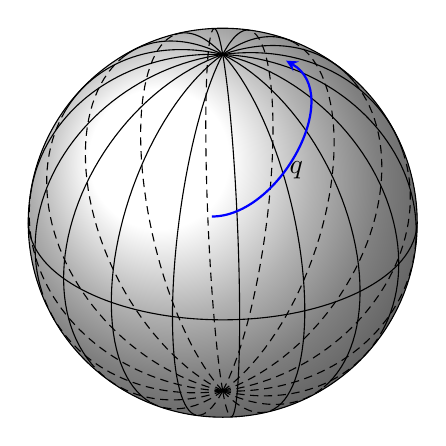
\begin{tikzpicture}
    \pgfplotsset{compat=1.9}
        \def\tilt{45}
        \def\azimuth{30}
        \begin{axis}[%
        axis equal,
        width=14cm,
        height=14cm,
        hide axis,
        enlargelimits=0.3,
        view/h=\tilt,
        view/v=\azimuth,
        scale uniformly strategy=units only,
        colormap={bluewhite}{color=(blue) color=(white)}]
        \coordinate (X) at (axis cs: 1,0,0);
        \coordinate (-X) at (axis cs: -1,0,0);
        \coordinate (Y) at (axis cs: 0,1,0);
        \coordinate (-Y) at (axis cs: 0,-1,0);
        \coordinate (Z) at (axis cs: 0,0,1);
        \coordinate (-Z) at (axis cs: 0,0,-1);
        \filldraw[ball color=white] (axis cs: 0,0,0) circle (2.47cm);
        \pgfplotsinvokeforeach {0}{
        \pgfplotsextra{ 
        \pgfmathsetmacro\sinVis{sin(#1)/cos(#1)*sin(\azimuth)/cos(\azimuth)}
         % angle of "visibility"
        \pgfmathsetmacro\angVis{asin(min(1,max(\sinVis,-1)))}
        \coordinate (X) at (axis cs: {cos(#1)},0,{sin(#1)});
        \draw (X) arc (0:\tilt+\angVis:{100*cos(#1)}) (X) arc (0:-180+\tilt-\angVis:{100*cos(#1)});}}
        \foreach \a in {0,20,...,359}
        {\pgfmathsetmacro{\Bound}{-60*cos(\a+45)}
        \addplot3[domain=\Bound:90, samples=45,samples y=0] ({cos(\a)*cos(x)},{sin(\a)*cos(x)},{sin(x)});
        \addplot3[domain=-90:\Bound, samples=45,samples y=0, densely dashed] ({cos(\a)*cos(x)},{sin(\a)*cos(x)},{sin(x)});}
        \draw[draw=blue,>={stealth[blue]},->,thick] (3.2cm,3.5cm,3.5cm) to [in = 330, out=0] node [below] {$q$} (2.0cm,6.6cm,5cm);
        \end{axis}
    \end{tikzpicture}
    \caption{How to construct $L(p,q)$.}
    \label{fig:surgery_theory_lens_space_drawing}
\end{figure}
We move on to the structure set of topological spaces, in particular closed topological manifolds $\mathcal{M}$.
\begin{definition}
Equivalent homotopies are homotopy equivalences $f_{1}:X_{1}\rightarrow Y$, $f_{2}:X_{2}\rightarrow Y$, denoted $f_{1}\sim f_{2}$, such that there exists a continuous function $g:X_{1}\rightarrow X_{2}$ and $f_{2}\circ g \simeq f_{1}$.
\end{definition}
The equivalent classes of $Y$ is called the structure set of $Y$. This set contains maps like $f_{1},f_{2}$. If $g$ is a homeomorphism, then $f_{1} = f_{2}$.
\begin{example}
$S(S^{n}) = \{S^{n}\}$
\end{example}
If $|S(Y)|>1$, then $Y$ is non-rigid.
\begin{example}
$|S(L(p,q))| \ne 1$
\end{example}
A few questions naturally arise from the definition of the structure set:
\begin{enumerate}
\begin{multicols}{2}
    \item Is $S(Y)$ a group?
    \begin{itemize}
        \item Sometimes.
    \end{itemize}
    \item Is $S(Y)$ fininte?
    \begin{itemize}
        \item Sometimes.
        \begin{itemize}
            \item $|S(S^{n})| = 1$
            \item $|S(T^{n})| = 2^{n}$
        \end{itemize}
    \end{itemize}
    \item Can $S(Y)$ be infinite?
    \begin{itemize}
        \item Yes.
        \begin{itemize}
            \item $|S(\mathbb{RP}^{5})|$ - Finite.
            \item $|S(\mathbb{RP}^{6})|$ - Finite.
            \item $|S(\mathbb{RP}^{7})|$ - \underline{Infinite}.
            \item $|S(\mathbb{RP}^{8})|$ - Finite.
        \end{itemize}
    \end{itemize}
\end{multicols}
\end{enumerate}
A review of some concepts from algebraic topology.
\begin{definition}
A path in a topological space $X$ is a continuous function $f:I\rightarrow X$
\end{definition}
\begin{definition}
A loop in a topological space $X$ is a path $f$ such that $f(0)=f(1)$.
\end{definition}
\begin{definition}
The fundamental group of a topological space $X$ is the set $\pi_{1}(X) = \{f\in C(I,X):f(0) = f(1)\}/h$, where $h$ is the modulo of homotopy, equipped with the concatenation operation:
\begin{equation*}
    (f*g)(t) = \begin{cases} f(2t), & 0\leq t < \frac{1}{2}\\ g(2t-1), & \frac{1}{2}\leq t < 1\end{cases}
\end{equation*}
\end{definition}
\begin{example}
\begin{align*}
    \begin{rcases*} \pi_{1}(S^{n}) = \{e\}\\ \pi_{1}(T^{n}) = \mathbb{Z}^{n} \end{rcases*} \textrm{No Torsion}\\
    \begin{rcases*} \pi_{1}(\mathbb{RP}^{n}) = \mathbb{Z}_{2} \\ \pi_{1}(L(p,q)) = \mathbb{Z}_{p} \end{rcases*} \textrm{Torsion}
\end{align*}
\end{example}
\begin{definition}
The order of an element $g$ of a group $G$ is $O(g) = \inf\{n\in \mathbb{N}:a = a^{n}\}$.
\end{definition}
\begin{definition}
A torsion group is a group $G$ such that there exists $g\in G$ such that $1<O(g)<\infty$.
\end{definition}
We now arrive at the first ``Surgery Theory" based theorem.
\begin{theorem}
If $n\geq 5$, $n\equiv 3\! \mod 4$, and $\pi_{1}(X)$ is a torsion group, then $|S(X^{n})| = \infty$.
\end{theorem}
Some other gems: $S(\mathbb{C}\mathbb{P}^{n}) = \mathbb{Z}_{2}$. Chern Manifolds are a thing.
\subsubsection{The Unsolvable Word Problem}
\begin{definition}
A presentation of a group $G$ is a set $H\subset G$ of generators and a set $R$ of relations on $H$. This is denoted $G = \langle H|S\rangle$.
\end{definition}
\begin{example}
\begin{enumerate}
    \item $\langle a | a^{n} = e\rangle$ is a the cyclic group of order $n$ generated by $a$.
    \item $\langle g,h|hg = gh\rangle = \mathbb{Z}^{2}$
    \item $\langle g,h|g^{2} = e, h^{2} = e\rangle = \mathbb{Z}_{2}*\mathbb{Z}_{n}$
    \item $\langle g,h|f^{2} = e,h^{2} = e, gh=h^{-1}g\rangle = D_{2n}$
\end{enumerate}
\end{example}
\begin{remark}
The word problem on unsolvability: Given two group presentations, there is no algorithm to show that they are isomorphic.
\end{remark}
\begin{definition}
A finitely presented group is a group with a presentation $\langle H|R\rangle$ such that $H$ and $R$ are finite.
\end{definition}
\begin{theorem}
If $n\geq 5$ and $G$ is finitely presented, then there is a closed $n$ dimensional manifold $\mathcal{M}$ such that $\pi_{1}(\mathcal{M}) = G$.
\end{theorem}
\subsubsection{Exact Sequences and Surgery Exact Sequences}
\begin{definition}
An exact sequence $\cdots G_{3}\overset{f_{3}}{\rightarrow}G_{2}\overset{f_{2}}{\rightarrow}G_{1}\overset{f_{1}}{\rightarrow}G_{0}$ is a sequence $f_{n}$ of homomorphisms and a sequence $G_{n}$ of groups such that $\Im(f_{n+1}) = \ker(f_{n})$
\end{definition}
\begin{remark}
Note, the definition requires that the $f_{n}$ are \textit{homomorphisms}, not homeomorphisms. Homeomorphism is a topological notion, not an algebraic one.
\end{remark}
\begin{example}
$O\overset{f}{\rightarrow}G\overset{g}{\rightarrow}H$. $\Im(f) = 0$, $\ker(g) = 0$. So $g$ is injective.
\end{example}
\begin{example}
$G\overset{f}{\rightarrow}H\overset{g}{\rightarrow}O$, $\ker(g) = H$, $\Im(f) = H$, $f$ is surjective.
\end{example}
\begin{definition}
A short exact sequence is an exact sequence $0\overset{f}{\rightarrow}G\overset{g}{\rightarrow}H\overset{h}{\rightarrow}L\overset{f_{3}}{\rightarrow}0$
\end{definition}
We have, from the previous examples, than in an exact sequence $f$ must be injective and $g$ must be surjective. We now move onto surgery exact sequences (See Wall et. al). Let $n\geq 5$, and $\mathcal{M}$ be a closed manifold of dimension $n$. Let $\pi = \pi_{1}(\mathcal{M})$. Let Cat have the following meaning:
\begin{itemize}
    \item Top: Category of continuous maps. That is, the topological catagory.
    \item PL: Piece-Wise linear category. Maps are piece-wise linear.
    \item Diff: Differentiable category. Maps are diffeomorphisms.
\end{itemize}
\begin{example}
\
\begin{enumerate}
    \begin{multicols}{2}
        \item $S^{Top}(S^{n}) = \{S^{n}\}$
        \item $S^{PL}(S^{n}) = \{S^{n}\}$
        \item $|S^{Diff}(S^{2})| = 28$ (Milnor)
        \item $S^{PL}(T^{n}) = \{S^{n}\}$ - Rigid
        \item $|S^{PL}(T^{n})| = 2^{n}$ - Non-Rigid.
        \item $S^{Diff}(T^{n})$ - Unknown.
    \end{multicols}
\end{enumerate}
\end{example}
A surgery exact sequence is a sequence of the form:
\begin{align*}
    S^{Cat}(M\times S') \rightarrow [M\times S',G/Cat] &\rightarrow L_{n+1}(\pi_{1}(\mathcal{M})) \rightarrow S^{Cat}(\mathcal{M}) \rightarrow \cdots\\
    \cdots &\rightarrow [M,G/Cat] \rightarrow L_{n}(\pi_{1}(\mathcal{M}))
\end{align*}
Here, $L_{n}(X)$ is a \textit{Wall Group}, and $[A,B]$ is a type of classifiying space.
\subsection{Lecture 2: Surgery Structure Sets}
\begin{wrapfigure}[6]{r}{0.2\textwidth}
\vspace{-6ex}
\centering
\begin{tikzcd}[row sep=small,column sep=large]
N_{1} \arrow[dd,"g"] \arrow[dr, "f_{1}"] \\
& M \\
N_{2} \arrow[ur, "f_{2}" below]
\end{tikzcd}
\caption[Surgery Theory Commutative Diagram]{Commutative Diagram for $g$}
\label{fig:wellesley_surgery_theory_commutative_diagram_for_g_for_two_homotopy_equivalences}
\end{wrapfigure}
Let $X,M_{1}$, and $M_{2}$ be closed, compact $n$-dimensional manifolds without boundary. Two homotopy equivalences $f_{i}:M_{i}\rightarrow X$ are called equivalent if there exists a cobordism $(W;M_{1},M_{2})$ and a map $(F;f_{1},f_{2}):(W;M_{1},M_{2})\rightarrow (X\times [0,1];X\times \{0\},X\times\{1\})$ such that $F,f_{1},f_{2}$ are homotopy equivalences. The structure set $S(X)$ is the set of equivalence classes of homotopy equivalences $f:M\rightarrow X$ from closed manifolds of dimension $n$ to $X$.\hfill
\begin{definition}
The surgery structure set of a closed (without boundary) compact manifold $M$ is $S(M) = \{f:N^{n}\rightarrow M^{n}|f\textrm{ is a Homotopy Equivalence}\}$
\end{definition}
\begin{definition}
The base point of a surgery structure set is the map $id_{X}:X\rightarrow X$.
\end{definition}
Let $N_{1}$ and $N_{2}$ be two manifold structures. And let $f_{1}:N_{1}^{n}\rightarrow M^{n}$ and $f_{2}:N_{2}^{n}\rightarrow M^{n}$ be two homotopy equivalences. We call $g:N_{1}\rightarrow N_{2}$ a cat-homeomorphism if $g$, together with $f_{1}$ and $f_{2}$, form the commutative diagram in figure \ref{fig:wellesley_surgery_theory_commutative_diagram_for_g_for_two_homotopy_equivalences}. That is, $g$ is a cat-homeomorphism if it homotopoy commutes.
\begin{remark}
Cat means category. There are three types: Top, PL, and Diff. 
    \begin{itemize}
        \begin{multicols}{3}
            \item Top: Topological
            \item PL: Piece-wise Linear
            \item Diff: Diffeomorphism
        \end{multicols}
    \end{itemize}
\end{remark}
\begin{example}
Some examples of surgery structure sets:
    \begin{enumerate}
        \begin{multicols}{3}
            \item $S^{Top}(S^{n})=\{S^{n}\}$
            \item $S^{PL}(S^{n}) = \{S^{n}\}$
            \item $S^{Diff}(S^{7}) = \mathbb{Z}_{28}$
        \end{multicols}
    \end{enumerate}
\end{example}
\subsubsection{Orientable and Non-Orientable}
Stiefel-Whitney classes $w_{1},\hdots, w_{n}$ are cohomological classes. Orientiable means that $w_{1} = 0$.
\begin{example}
\
\begin{enumerate}
    \begin{multicols}{2}
    \item $\mathbb{RP}^{2}$ - Non-Orientable
    \item $\mathbb{RP}^{4}$ - Non-Orientable
    \item $\mathbb{RP}^{6}$ - Non-Orientable
    \item $\mathbb{RP}^{8}$ - Non-Orientable
    \item $\mathbb{RP}^{3}$ - Orientable
    \item $\mathbb{RP}^{5}$ - Orientable
    \item $\mathbb{RP}^{7}$ - Orientable
    \item $\mathbb{CP}^{n}$ - Orientable for all $n\in\mathbb{N}$
    \end{multicols}
\end{enumerate}
\end{example}
Returning to surgery exact sequences, the goal is to compute $S^{Cat}(\mathcal{M}^{n})$, where $n$ is the dimension of $\mathcal{M}^{n}$. The notion of a surgery helps solve this question. Let $X = \mathbb{S}^{2}\setminus\{(a_{1},b_{1},c_{1}),(a_{2},b_{2},c_{2})\}$. That is, the sphere with two points removed. Stretch these two points out to create a sphere with two holes removed. One could imagine taking a hollow cylinder and stretching it to connect the two holes in the sphere. The result is a spherical coffee cup, as shown in Fig.~\ref{fig:surgery_theory_example_of_a_surgery}. This figure can be continuously deformed into a torus.
\begin{figure}[H]
    \centering
    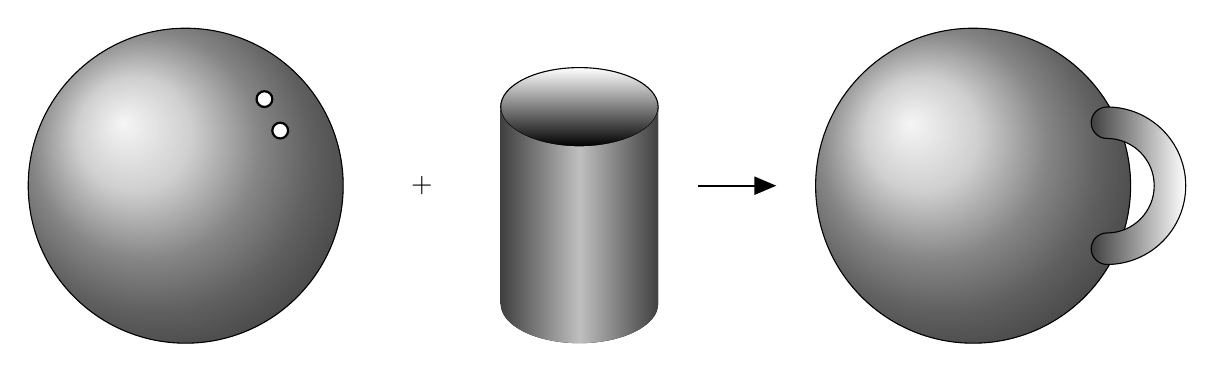
\begin{tikzpicture}
        \fill[ball color = gray!50!white,draw=black] (0,0) circle (2);
        \fill[fill=white,draw=black,thick] (1,1.1) circle (0.1);
        \fill[fill=white,draw=black,thick] (1.2,0.7) circle (0.1);
        \node at (3,0) {$+$};
        \fill[bottom color = black,top color = white,draw=black] (5,1) ellipse (1 and 0.5);
        \fill[left color=gray!50!black,right color=gray!50!black,middle color=gray!50,shading=axis] (4,1) -- (4,-1.5) arc(180:360:1 and 0.5) -- (6,1) arc(360:180:1 and 0.5);
        \draw[draw=black,thick,>=triangle 45,->] (6.5,0) -- (7.5,0);
        \fill[ball color = gray!50!white,draw=black] (10,0) circle (2);
        \fill[left color=black!50!gray,right color=white,draw=black,thin] (11.7,1) arc(90:-90:1) arc(-90:-270:0.2) arc(-90:90:0.6) arc(-90:-270:0.2);
    \end{tikzpicture}
    \caption{Caption}
    \label{fig:surgery_theory_example_of_a_surgery}
\end{figure}
Recall that $S^{0}$ is two points, and that $D^{2}$ is the open unit disc. Then $S^{0}\times D^{2}$ is simply two disjoint open unit discs. This is a good representation of the idea of the disjoint union, denoted $X\coprod Y$. We have that:
\begin{equation*}
    S^{0}\times D^{2} = D^{2} \coprod D^{2}
\end{equation*}
We can also represent a cylinder as the closed $S^{1}\times \overline{D}^{1}$. The codimension of a surgery is the dimension of the object minus the dimension of a surgery. So, for the surgery in Fig.~\ref{fig:surgery_theory_example_of_a_surgery}, the dimension of the entire thing is $2$, the dimension of the surgery is $2$, so the codimension is $0$. This is called a Zero-Surgery. A zero-surgery takes out $2$ holes and connects them with a tube.
\begin{figure}[H]
    \centering
    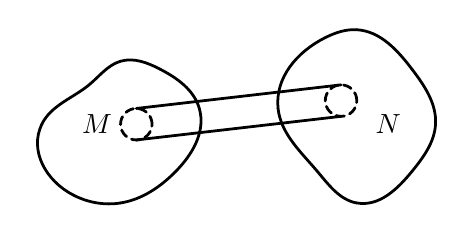
\begin{tikzpicture}[line width=1pt,line cap = round,>={Stealth[black]},every edge/.style={draw=black,very thick}]
        \node[fill=black,circle,inner sep=0pt,outer sep=0pt] at (0,0) (a) {};
        \node[fill=black,circle,inner sep=0pt,outer sep=0pt] at (-0.6,0.1) (b) {};
        \node[fill=black,circle,inner sep=0pt,outer sep=0pt] at (-1,1) (c) {};
        \node[fill=black,circle,inner sep=0pt,outer sep=0pt] at (-0.4,1.5) (d) {};
        \node[fill=black,circle,inner sep=0pt,outer sep=0pt] at (0, 1.8) (e) {};
        \node[fill=black,circle,inner sep=0pt,outer sep=0pt] at (0.5, 1.7) (f) {};
        \node[fill=black,circle,inner sep=0pt,outer sep=0pt] at (1,1.2) (g) {};
        \node[fill=black,circle,inner sep=0pt,outer sep=0pt] at (0.7,0.4) (h) {};
        \node at (-0.3,1) (i) {$M$};
        \path[draw,use Hobby shortcut,closed=true](a) .. (b) .. (c) .. (d) .. (e) .. (f) .. (g) .. (h);
        \node[fill=black,circle,inner sep=0pt,outer sep=0pt] at (3,0) (a1) {};
        \node[fill=black,circle,inner sep=0pt,outer sep=0pt] at (2.5,0.4) (b1) {};
        \node[fill=black,circle,inner sep=0pt,outer sep=0pt] at (2,1.2) (c1) {};
        \node[fill=black,circle,inner sep=0pt,outer sep=0pt] at (2.6,2.1) (d1) {};
        \node[fill=black,circle,inner sep=0pt,outer sep=0pt] at (3, 2.2) (e1) {};
        \node[fill=black,circle,inner sep=0pt,outer sep=0pt] at (3.7, 1.7) (f1) {};
        \node[fill=black,circle,inner sep=0pt,outer sep=0pt] at (4,1) (g1) {};
        \node[fill=black,circle,inner sep=0pt,outer sep=0pt] at (3.7,0.4) (h1) {};
        \node at (3.4,1) (i1) {$N$};
        \draw[draw=black,densely dashed] (0.2,1) circle (0.2);
        \draw[draw=black,densely dashed] (2.8,1.3) circle (0.2);
        \draw (0.2,1.2) -- (2.8,1.5);
        \draw (0.2,0.8) -- (2.8,1.1);
        \path[draw,use Hobby shortcut,closed=true](a1) .. (b1) .. (c1) .. (d1) .. (e1) .. (f1) .. (g1) .. (h1);
    \end{tikzpicture}
    \caption[Surgery Theory - A Zero Surgery]{A Zero Surgery between $N$ and $M$.}
    \label{fig:surgery_theory_a_zero_surgery}
\end{figure}
Let $\mathcal{M}^{n}$ be an $n$ dimensional manifold. Embed $S^{k}\times D^{n-k}$ into $\mathcal{M}^{n}$. Then $\partial(S^{k}\times D^{n-k}) = S^{k}\times S^{n-k-1}$, where $\partial(X)$ is the boundary of $X$. Remove $\partial(S^{k}\times D^{n-k})$ and glue $S^{k+1}D^{n-k-1}$. Note that $\dim(S^{k+1}\times D^{n-k-1}) = \dim(S^{k}\times D^{n-k}) = n$. We alse have that $\partial(D^{k+1}\times S^{n-k-1}) = S^{k}\times S^{n-k-1}$. Glue $\mathcal{M}^{n}\cup (D^{k+1}\times S^{n-k-1})$ along $\partial(S^{k}\times S^{n-k-1})$.
\begin{figure}[H]
    \centering
    \resizebox{!}{0.2\textheight}{
    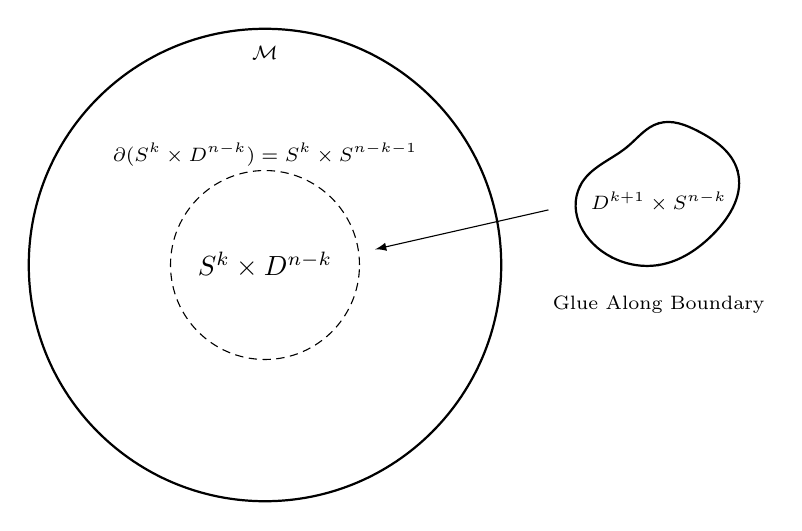
\begin{tikzpicture}
        \draw[draw=black,densely dashed] (0,0) circle (1.2);
        \draw[draw=black,thick] (0,0) circle (3);
        \node at (0,2.7) {\scriptsize{$\mathcal{M}$}};
        \node at (0,0) {$S^{k}\times D^{n-k}$};
        \node at (0,1.4) {\scriptsize{$\partial(S^{k}\times D^{n-k}) = S^{k}\times S^{n-k-1}$}};
        \node[fill=black,circle,inner sep=0pt,outer sep=0pt] at (5,0) (a) {};
        \node[fill=black,circle,inner sep=0pt,outer sep=0pt] at (4.4,0.1) (b) {};
        \node[fill=black,circle,inner sep=0pt,outer sep=0pt] at (4,1) (c) {};
        \node[fill=black,circle,inner sep=0pt,outer sep=0pt] at (4.6,1.5) (d) {};
        \node[fill=black,circle,inner sep=0pt,outer sep=0pt] at (5, 1.8) (e) {};
        \node[fill=black,circle,inner sep=0pt,outer sep=0pt] at (5.5, 1.7) (f) {};
        \node[fill=black,circle,inner sep=0pt,outer sep=0pt] at (6,1.2) (g) {};
        \node[fill=black,circle,inner sep=0pt,outer sep=0pt] at (5.7,0.4) (h) {};
        \node at (5,0.8) {\scriptsize{$D^{k+1}\times S^{n-k}$}};
        \draw[>=latex,draw=black,->] (3.6,0.7) -- (1.4,0.2);
        \node at (5,-0.5) {\scriptsize{Glue Along Boundary}};
        \path[draw,use Hobby shortcut,closed=true,thick](a) .. (b) .. (c) .. (d) .. (e) .. (f) .. (g) .. (h);
    \end{tikzpicture}}
    \caption[Surgery Theory - Surgery Example]{Gluing $D^{k+1}\times S^{n-k}$ along $\partial(S^{k}\times D^{n-k})$. The new manifold is $\mathcal{M}^{n}\setminus (S^{k}\times D^{n-k}\coprod (D^{k+1}\times S^{n-k-1})$}
    \label{fig:surgery_theory_glueing_S_k_D_n_k_to_M}
\end{figure}
We now consider $k$ surgeries $\mathcal{M}\overset{\textrm{k-surgery}}{\longrightarrow}\mathcal{N}$.  We have seen $S^{2}\overset{\textrm{0-surgery}}{\longrightarrow} T^{2}$. Note: $\pi_{1}(S^{2})$ is trivial, and $\pi_{1}(T^{2}) = \mathbb{Z}^{2}$. This happens because $n<5$. When $n\geq 5$, we have the following result.
\begin{theorem}
If $\mathcal{M}$ is an $n$ dimensional manifold, $n\geq 5$, and if $\mathcal{N}$ is the result of a $k$ surgery on $\mathcal{M}$, then $\pi_{1}(\mathcal{M}) = \pi_{1}(\mathcal{N})$.
\end{theorem}
\subsubsection{More On Surgery Exact Sequences}
Recall that a surgery exact sequence looks like the following:
\begin{equation*}
    \underset{\textrm{Group}}{\underbrace{L_{n+1}(\mathbb{Z}\pi_{1}\mathcal{M})}} \rightarrow \cdots \rightarrow \underset{\textrm{Not a Group}}{\underbrace{S^{Cat}(\mathcal{M}^{n})}} \rightarrow \underset{\textrm{Group}}{\underbrace{[M,G/0]}} \rightarrow \underset{\textrm{Group}}{\underbrace{L_{n}(\mathbb{Z}\pi_{1}(\mathcal{M}))}} 
\end{equation*}
An exact sequence of groups is of then form $G_{n+1}\overset{g_{n}}{\rightarrow} G_{n}\rightarrow \hdots$, where $\Im(g_n) = \ker(g_{n-1})$. We refine our notion of a surgery exact sequence:
\begin{equation*}
    \cdots \rightarrow L_{n+1}(\mathbb{Z}\pi_{1}(\mathcal{M})) \dashrightarrow S^{Cat}(\mathcal{M}) \overset{g}{\rightarrow} [M,G/o] \overset{\sigma}{\rightarrow} L_{n}(\mathbb{Z}\pi_{1}(\mathcal{M}))
\end{equation*}
The dotted line means $L_{n+1}(\mathbb{Z}\pi_{1}(\mathcal{M}))$ acts on $S^{Cat}(\mathcal{M})$. Exact means that $\Im(g) = \ker(\sigma)$. Each element $f\in [M,G/o]$ either pulls back to $\emptyset$ or something non-empty. If non-empty, you get a blob in $S^{Cat}(\mathcal{M})$: $f^{-1}(\{x\})$. But:
\begin{equation*}
    \underset{f\in [M,G/o]}{\cup}g^{-1}(\{f\}) = S^{Cat}(\mathcal{M})
\end{equation*}
This process creates a partition of $S^{Cat}(\mathcal{M})$. Now, $L_{n+1}(\mathbb{Z}(\pi_{1}\mathcal{M}))$ acts on $S^{Cat}(\mathcal{M})$ in some fashion. Partition the space into orbits. Exactness here means that partitioning by point inverses is the same as partitioning by orbits. That is, the two partitions are identical. See Fig.~\ref{fig:surgery_theory_partition_of_S_Cat} for a partioning into orbits.
\begin{figure}[H]
    \centering
    \resizebox{!}{0.15\textheight}{
    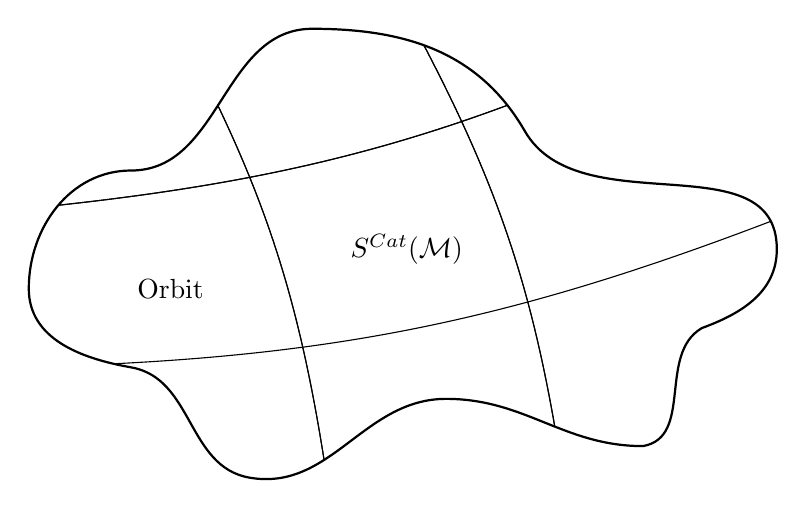
\begin{tikzpicture}
        \path coordinate (aux0) at (0,1.5) coordinate (aux1) at (0,3.5) coordinate (aux2) at (10,3.5) coordinate (aux3) at (9,6) coordinate (aux4) at (4,0) coordinate (aux5) at (7,0) coordinate (aux6) at (2,6) coordinate (aux7) at (5,6) coordinate (esp1) at (0.2,2.5) coordinate (esp2) at (1.5,1.5) coordinate (esp3) at (3,0.1) coordinate (esp4) at (5.5,1.1) coordinate (esp5) at (8,0.5) coordinate (esp6) at (8.75,2) coordinate (esp7) at (9.7,3) coordinate (esp8) at (6.5,4.5) coordinate (esp9) at (3.8,5.8) coordinate (esp10) at (1.5,4);
        \draw[line width=0.8pt] (esp1) to[out=-90,in=170] (esp2) to[out=-10,in=170] (esp3) to[out=-10,in=180] (esp4) to[out=0,in=180] (esp5) to[out=10,in=-150] (esp6) to[out=20,in=-90] (esp7) to[out=90,in=-60] (esp8) to[out=120,in=0] (esp9) to[out=180,in=0] (esp10) to[out=180,in=90] cycle;    
        \clip (esp1) to[out=-90,in=170] (esp2) to[out=-10,in=170] (esp3) to[out=-10,in=180] (esp4) to[out=0,in=180] (esp5) to[out=10,in=-150] (esp6) to[out=20,in=-90] (esp7) to[out=90,in=-60] (esp8) to[out=120,in=0] (esp9) to[out=180,in=0] (esp10) to[out=180,in=90] cycle;
        \draw (aux4) to[bend right=10] (aux6) -- (aux7) to[bend left=10] (aux5) -- cycle;
        \draw (aux5) to[bend right=10] (aux7) -- (10,6) -- (10,0) -- cycle;
        \draw (aux0) -- (aux1) to[bend right=10] (aux3) -- (10,6) -- (aux2) to[bend left=10] cycle;
        \draw (0,0) -- (aux4) to[bend right=10] (aux6) -- (0,6) -- (0,0) -- cycle;
        \draw (0,6) -- (aux1) to[bend right=10] (aux3) -- (0,6) -- cycle;
        \node at (2,2.5) {Orbit};  
        \node at (5,3) {$S^{Cat}(\mathcal{M})$};
        \end{tikzpicture}}
    \caption[Surgery Theory - Partion of $S^{Cat}$]{Partition of $S^{Cat}(\mathcal{M})$}
    \label{fig:surgery_theory_partition_of_S_Cat}
\end{figure}
The next object to talk about is $L_{n}(\mathbb{Z}\pi_{1}(\mathcal{M}))$. These are called Wall groups. They are difficult to compute, but there are some facts that are known about them:
\begin{itemize}
    \item Wall groups only have 2-torsion.
    \begin{itemize}
        \item 2-torsion means that elements of finite order have order $2$.
        \item This implies the groups are Abelian.
    \end{itemize}
    \item They can be orientable or not.
    \begin{itemize}
        \item $L_{n}(\mathbb{Z}\pi_{1}(\mathcal{M})^{\pm})$ indicates orientable or not.
    \end{itemize}
\end{itemize}
\subsection{Lecture 3: Vector Bundles and Group Rings}
\subsection{Lecture 4: Principle G-Bundles}
A brief discussion on complexes. A simplex is a generalization of the notation of a triangle. A triangle can be considered as the convex-hull of $3$ non-coplanar points. This is called a $2$-simplex. A $0$-simplex is thus a point, and a $1$-simplex is a line. This can be generalized into higher dimensions as well. A $3$-simplex is a tetrahedron, and an $n$-simplex is an $n$ dimensional triangle, defined on $n+1$ non-hyper-coplanar points.
\begin{figure}[H]
    \centering
    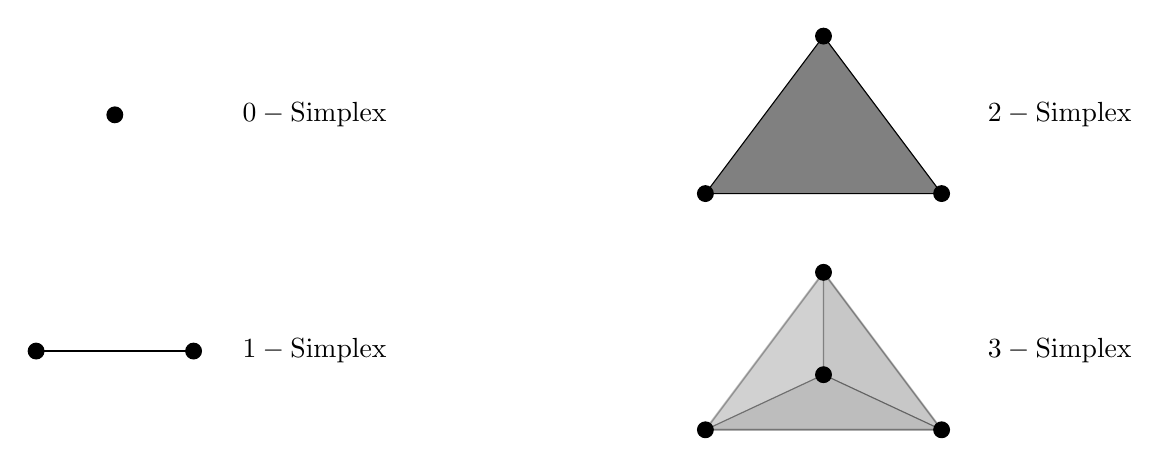
\begin{tikzpicture}
        \filldraw[draw=black,fill=black] (0,1) circle (0.1);
        \node at (1.5,1) [right] {$0-\textrm{Simplex}$};
        \filldraw[draw=black,fill=black] (-1,-2) circle (0.1);
        \filldraw[draw=black,fill=black] (1,-2) circle (0.1);
        \draw[draw=black,semithick] (1,-2) -- (-1,-2);
        \node at (1.5,-2) [right] {$1-\textrm{Simplex}$};
        \filldraw[fill=gray] (9,2) -- (7.5,0) -- (10.5,0) -- cycle;
        \filldraw[draw=black,fill=black] (9,2) circle (0.1);
        \filldraw[draw=black,fill=black] (7.5,0) circle (0.1);
        \filldraw[draw=black,fill=black] (10.5,0) circle (0.1);
        \node at (12,1) {$2-\textrm{Simplex}$};
        \filldraw[draw=black,fill=gray,opacity=0.2] (9,-1) -- (7.5,-3) -- (9,-2.3) -- cycle;
        \filldraw[draw=black,fill=gray,opacity=0.3] (9,-1) -- (10.5,-3) -- (9,-2.3) -- cycle;
        \filldraw[draw=black,fill=gray,opacity=0.4] (9,-2.3) -- (7.5,-3) -- (10.5,-3) -- cycle;
        \filldraw[draw=black,fill=gray,opacity=0.2,thick] (9,-1) -- (7.5,-3) -- (10.5,-3) -- cycle;
        \filldraw[draw=black,fill=black] (9,-1) circle (0.1);
        \filldraw[draw=black,fill=black] (7.5,-3) circle (0.1);
        \filldraw[draw=black,fill=black] (10.5,-3) circle (0.1);
        \filldraw[draw=black,fill=black] (9,-2.3) circle (0.1);
        \node at (12,-2) {$3-\textrm{Simplex}$};
    \end{tikzpicture}
    \caption[Surgery Theory - Simplices]{Examples of Simplices}
    \label{fig:surgery_theory_simplexes}
\end{figure}
A simplicial complex is a set of simplices $\mathcal{H}$ such that the face of any element of $\mathcal{H}$ is also contained in $\mathcal{H}$, and the intersection of two simplices $\sigma_{1},\sigma_{2}\in \mathcal{K}$ is a face of both $\sigma_{1}$ and $\sigma_{2}$. We return to studying surgery exact sequences for $n\geq 5$. Let $\mathcal{M}$ be an $n$ dimensional manifold, and let $G = \pi_{1}(\mathcal{M})$. In our surgery exact sequence we still have this mysterious object $[\mathcal{M},G/Cat]$. Let Cat be either PL or Top. The generalized Poincare Conjecture says that, for $n\geq 5$, $S^{PL}(S^{n}) = S^{Top}(S^{n}) = \{S^{n}\}$. Let $\mathcal{M} = S^{n}$. Then $G = \pi_{1}(\mathcal{M}) = \{e\}$. Then we have the following:
\begin{figure}[H]
    \centering
    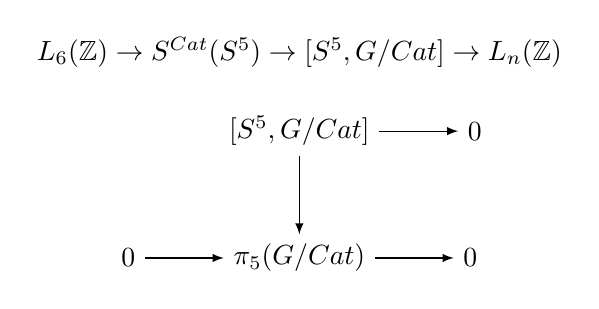
\begin{tikzpicture}[>=latex]
        \node (a) {$[S^{5},G/Cat]$};
        \node (b) [right=of a] {$0$};
        \node (c) [below=of a] {$\pi_{5}(G/Cat)$};
        \node (d) [right=of c] {$0$};
        \node (e) [left=of c] {$0$};
        \node (TEXT) [above=2cm of c] {$L_{6}(\mathbb{Z})\rightarrow S^{Cat}(S^{5}) \rightarrow [S^{5},G/Cat] \rightarrow L_{n}(\mathbb{Z})$};
        \path[->] (a) edge (b);
        \path[->] (c) edge (d);
        \path[->] (e) edge (c);
        \path[->] (a) edge (c);
    \end{tikzpicture}
    \caption[Surgery Theory - Diagram for Sequence of $S^{5}$]{Digram for the Surgery Exact Sequence of $S^{5}$}
    \label{fig:surgery_theory_example_diagram_for_surgery_exact_sequence}
\end{figure}
So, $\pi_{5}(G/Cat) = \{e\}$. This gives us:
\begin{align*}
    \cdots \rightarrow S^{Cat}(S^{6})\rightarrow [S^{6},G/Cat] &\rightarrow L_{6}(\mathbb{Z}) \rightarrow \cdots\\
    \cdots &\rightarrow 0 \rightarrow \pi_{6}(G/Cat) \rightarrow \mathbb{Z}_{2}\rightarrow 0
\end{align*}
So, we have $\pi_{6}(G/Cat) \cong \mathbb{Z}_{2}$. In general, $\pi_{n}(G/o) \cong L_{n}(\mathbb{Z})$.
\begin{theorem}[Wall's Theorem]
\begin{equation*}
    L_{n}(\mathbb{Z}) = \begin{cases} \mathbb{Z}, & n \equiv 0 \mod 4 \\ 0, & n \equiv 1 \mod 4 \\ \mathbb{Z}_{2}, & n \equiv 2 \mod 4 \\ 0, & n \equiv 3 \mod 4 \end{cases}
\end{equation*}
\end{theorem}
All $L$ groups are periodic, and never have odd torsion. That is, there is never $\mathbb{Z}_{3},\mathbb{Z}_{5}$, etc. Wall groups are hard to compute. Whatever $G/Cat$ is, its homotopy groups for $n\geq 5$ are known.
\subsubsection{Principle G-Bundles}
A few things are needed:
\begin{itemize}
    \item Map $p:E\rightarrow X$, where $E$ is a total space and $X$ is a base space.
    \item The inverse-image $E_{x} = p^{-1}(\{x\})$ is called the fiber over $x$.
    \item $G$ (Group) acts on each $E_{x}$ freely and transitively.
    \item $G$ has to act `continuously.' Nearby points are taken to nearby points.
\end{itemize}
Then $p:E\rightarrow X$ is a $G-$principle bundle.
\begin{remark}
Freely means the only element that fixes everything is the identity.
\end{remark}
\begin{example}
Take a sphere $S^{n}$ and a projection $p:S^{n} \rightarrow \mathbb{RP}^{n}$. $\mathbb{RP}^{n}$ is created by glueing antipotal points together. If $x\in \mathbb{RP}^{n}$, then $p^{-1}(\{x\})$ consists of $2$ antipotal points in $S^{n}$. Now $\mathbb{Z}_{2}$ acts on a sphere. $\mathbb{Z}_{2} = \{0,1\}$. $0$ maps $x \mapsto x$ and $1$ maps $x\mapsto -$. Note that $1+1 = 0$, as in $\mathbb{Z}_{2}$. Given any point, you can get to another point in the fiber. This is trivial in this example as there are only two points in the fiber. Also only the identity maps a point back to itself. This action is free and transitive, so $p:S^{n} \rightarrow \mathbb{RP}^{n}$ is a $\mathbb{Z}_{2}$-principle bundle.
\end{example}
\begin{remark}
Let $M$ be a manifold (Or a space) with dimension $n$ and fundamental group $G$. A universal cover $\tilde{M}$ of $M$ includes a map $p:\tilde{M}\rightarrow M$ such that $\tilde{M}$ is simply connected of dimension $n$, i.e. $\pi_{1}(\tilde{M}) = e$, and $\forall_{x\in M}$, $p^{-1}(x)$ is a collection of discrete points.
\end{remark}
\begin{remark}
$\pi_{1}(\mathbb{RP}^{n}) = \mathbb{Z}_{2}$ and $S^{n}$ is a universal cover of $\mathbb{RP}^{n}$. So this might come from a general theory.
\end{remark}
\begin{example}
Take the circle $S^{1}$. $\pi_{1}(S^{1}) = \mathbb{Z}$. There's a map $p(x) = e^{2\pi i x}$ of modulus $1$. Note that $p^{-1}(0) = \mathbb{Z}$. So $p^{-1}(x)$ is just a shift of $\mathbb{Z}$ $(\mathbb{Z}+r)$. Note that $\pi_{1}(\mathbb{R}) = e$. So $\mathbb{R}$ is a universal cover of $S^{1}$.
\end{example}
\begin{example}
We may think $\mathbb{R}^2$ is a universal cover of $S^{2}$, but $S^{2}$ is already simply connected. S $p$ is simply the identity map, and the universal cover of $S^{2}$ is simply $S^{2}$. All universal covers are homotopy equivalent.
\end{example}
\begin{remark}
Let $x\in M$. Then, for all $z\in p^{-1}(\{x\})$, and for all $g\in \pi_{1}(M)$, there is an action $gx\in p^{-1}(x)$. This uses the homotopy lifting property.
\end{remark}
There is an action $G$ on $\tilde{M}$ which preserves the fiber (Takes every element of a fiber to the same fiber. That is, it does not mix fibers), is transitive, and is free. The map $p:\tilde{M}\rightarrow M$ is a $\pi_{1}(M)-$Principal Bundle.
\subsubsection{Functors}
Let $F$ be a functor $F:\textit{Space}\rightarrow \textit{Groups}$. So for all spaces $X$, we have a group $F(X)$. There are many such examples:
\begin{itemize}
    \begin{multicols}{4}
        \item Cohomology
        \item Homology
        \item K-Theory
        \item Other Stuff
    \end{multicols}
\end{itemize}
\begin{remark}
Homology: Take $M$ and triangulate. Take maps from the simplicial complex of $M$ to $G$ (Group) (Certain conditions). There's an equivalence relation on these maps. That set after taking the equivalence relations is the homology: $H_{n}(M,G)$. $n$ describes the type of simplicies. If $n > \dim(M)$, then $H_{n}(G,M) = 0$. $H_{n}(M,G) = \{f:\Delta^{n}\rightarrow G\}$.
\end{remark}
\begin{remark}
Cohomology is the set $H^{n}(M,G) = [H_{n}(M,G),G]$, that is, the \textit{dual}.
\end{remark}
We want to talk about cohomology. Under special conditions there is something called the Brown Representation Theorem. Consider Cohomology $H^{n}(M,G)$, with coefficients in $G$. Cohomology is Homotopy invariant, that is if $M \cong N$, then $H^{n}(M,G) \cong H^{n}(N,G)$. The Brown-Representation Theorem says that there is a classifying space $BG$ such that, for all spaces $M$, there is a one-to-one correspondence between $H^{n}(X,G) \leftrightarrow [X,BG]$. In general, if $F$ is a functor, then the Brown-Representation Theorem says that there is a classifying space $Y$ such that $F(X)$ has a one-to-one correspondence with the homotopy classes of maps, $[X,Y]$. $F(x) \leftrightarrow [X,Y]$
\begin{example}
The Eilenberg-MacLane Space $K(G,n)$ has the property that, for all $j\ne n$, $\pi_{n}(K(G,n)) = G$, and $\pi_{j}(K(G,n)) = 0$. $K(G,n)$ is the classifying space for cohomology.
\end{example}
\begin{theorem}
$K(G,n)$ is the classifying space for cohomology. That is, up to homotopy, $H^{n}(X,G) \leftrightarrow [X,K(G,n)]$.
\end{theorem}
Let $\textrm{Prin}_{G}(X)$ be the collection of $G-$principal bundles on $X$. With a certain equivalence relation, it turns out the $\textrm{Prin}_{G}(X)$ is a group. So $\textrm{Prin}_{G}:\textit{Spaces}\rightarrow \textit{Groups}$ is a functor. The Brown-Representation Theorem implies that there is a classifying space $BG$ $\textrm{Prin}_{G}\leftrightarrow [X,BG]$.
\begin{theorem}
If $p:E\rightarrow X$ and $p':E'\rightarrow X$ are both bundles over $X$, then there exists $p\oplus p':E\oplus E' \rightarrow X$ COME BACK TO LATER
\end{theorem}
\subsubsection{Grothendique Groupification of Semigroup}
\begin{definition}
A semi-group is a group without the requirement for invereses.
\end{definition}
\begin{example}
$\{0,1,2,\hdots\}$ is a semi-group under addition.
\end{example}
Let $G$ be a semi-group. Constraint $G\times G/\sim$. $(a,b) \sim (c,d)$ if $a+d = b+c$. So, $(2,3)\sim (4,5) \sim (7,8)\sim (-1,0) \equiv -1$. The equivalence class of all of these things is called $-1$. We still have all of the positive integers, $(4,2)\sim(5,3) \sim(6,4) \equiv 2$. This process adds all of the negatives. This process, called Grothendique Construction on a Semi-group creates a group out of a semi-group. It is, in a way, the 'smallest' group containing the semi-group. The groupification of $\{0,1,2,3,\hdots\}$ will be $\mathbb{Z}$.
\begin{example}
What are the vector bundles over a dot? THere is $\mathbb{R}^{0}$ (A dot), $\mathbb{R}^{n}, \hdots,\mathbb{R}^n,\hdots $. There is an operation on this set $\{\mathbb{R}^{n}:n \geq 0\}$. This makes a semi-group, and there is a Grothendique Groupification $G_{r}(\mathbb{Z}_{\geq 0}, +) = \mathbb{Z}$
\end{example}
\part{Course Work: Physics}
\chapter{Electromagnetism I}
\section{Homework}
\subsection{Homework I}
Wangsness Chapter 1 - Problems: 2, 3, 4, 5, 8, 9
\begin{problem}[Wangsness 1-2]
Given $\mathbf{A} = 2\hat{\mathbf{x}}-3\hat{\mathbf{y}}-4\hat{\mathbf{z}}$ and $\mathbf{B} = 6\hat{\mathbf{x}}+5\hat{\mathbf{y}}+\hat{\mathbf{z}}$, find the magnitudes and angles made with the $x,y,$ and $z$ axes for $\mathbf{A}+\mathbf{B}$ and $\mathbf{A}-\mathbf{B}$.
\end{problem}
\begin{proof}[Solution]
First, we need to find $\mathbf{A}+\mathbf{B}$ and $\mathbf{A}-\mathbf{B}$:
\begin{align*}
    \mathbf{A}+\mathbf{B}&=(2\hat{\mathbf{x}}-3\hat{\mathbf{y}}-4\hat{\mathbf{z}})+(6\hat{\mathbf{x}}+5\hat{\mathbf{y}}+\hat{\mathbf{z}})&\mathbf{A}-\mathbf{B}&=(2\hat{\mathbf{x}}-3\hat{\mathbf{y}}-4\hat{\mathbf{z}})-(6\hat{\mathbf{x}}+5\hat{\mathbf{y}}+\hat{\mathbf{z}})\\
    &=(2+6)\hat{\mathbf{x}}+(5-3)\hat{\mathbf{y}}+(1-4)\hat{\mathbf{z}} & &=(2-6)\hat{\mathbf{x}}-(3+5)\hat{\mathbf{y}}-(4+1)\hat{\mathbf{z}}\\
    &=8\hat{\mathbf{x}}+2\hat{\mathbf{y}}-3\hat{\mathbf{z}} & &=-4\hat{\mathbf{x}}-8\hat{\mathbf{y}}-5\hat{\mathbf{z}}
\end{align*}
The magnitude of a vector $\mathbf{A} = a_{1}\hat{\mathbf{x}}_{1}+\hdots+a_{N}\hat{\mathbf{x}}_{N}$, also called its \textit{norm}, is:
\begin{equation*}
    \norm{\mathbf{A}}=\sqrt{\sum_{i=1}^{N}a_{i}^{2}}
\end{equation*}
Using this, we have:
\begin{align*}
    \norm{\mathbf{A+B}} &=(8^{2}+2^{2}+3^{3})^{1/2} &\norm{\mathbf{A-B}}&=(4^{2}+8^{2}+5^{2})^{1/2}\\
    &= \sqrt{77} & &=\sqrt{105}
\end{align*}
The \textit{direction angle} between $\mathbf{A}$ and the $\xi$-axis is $\alpha_{\xi}=\cos^{-1}\big(\frac{\mathbf{A}\cdot \hat{\boldsymbol{\upxi}}}{\norm{\mathbf{A}}\norm{\hat{\boldsymbol{\upxi}}}}\big) = \cos^{-1}\big(\frac{\mathbf{A}\cdot\hat{\boldsymbol{\upxi}}}{\norm{\mathbf{A}}}\big)$. The direction angles of $\mathbf{A}+\mathbf{B}$ and $\mathbf{A}-\mathbf{B}$ for $\hat{\mathbf{x}},\hat{\mathbf{y}}$, and $\hat{\mathbf{z}}$ are:
\begin{align*}
    \alpha &=\cos^{-1}\bigg(\frac{(\mathbf{A}+\mathbf{B})\cdot\hat{\mathbf{x}}}{\norm{\mathbf{A+B}}}\bigg) &\beta &= \cos^{-1}\bigg(\frac{(\mathbf{A}+\mathbf{B})\cdot \hat{\mathbf{y}}}{\norm{\mathbf{A}+\mathbf{B}}}\bigg) &\gamma&= \cos^{-1}\bigg(\frac{(\mathbf{A}+\mathbf{B})\cdot \hat{\mathbf{z}}}{\norm{\mathbf{A}+\mathbf{B}}}\bigg)\\
    &= \cos^{-1}\bigg(\frac{8}{\sqrt{77}}\bigg) & &= \cos^{-1}\bigg(\frac{2}{\sqrt{77}}\bigg) & &= \cos^{-1}\bigg(\frac{-3}{\sqrt{77}}\bigg)\\
    &= 24.3^{\circ} & &= 76.8^{\circ} & &= 110^{\circ}
\end{align*}
For $\mathbf{A}-\mathbf{B}$:
\begin{align*}
    \alpha &=\cos^{-1}\bigg(\frac{(\mathbf{A}-\mathbf{B})\cdot\hat{\mathbf{x}}}{\norm{\mathbf{A-B}}}\bigg)&\beta &= \cos^{-1}\bigg(\frac{(\mathbf{A}-\mathbf{B})\cdot\hat{\mathbf{y}}}{\norm{\mathbf{A}-\mathbf{B}}}\bigg) &\gamma&= \cos^{-1}\bigg(\frac{(\mathbf{A}-\mathbf{B})\cdot\hat{\mathbf{z}}}{\norm{\mathbf{A}-\mathbf{B}}}\bigg)\\
    &=\cos^{-1}\bigg(\frac{-4}{\sqrt{77}}\bigg) & &=\cos^{-1}\bigg(\frac{-8}{\sqrt{77}}\bigg) & &=\cos^{-1}\bigg(\frac{-5}{\sqrt{77}}\bigg)\\
    &=113^{\circ} & &=141.3^{\circ} & &=119.2^{\circ}
\end{align*}
\end{proof}
\begin{problem}[Wangsness 1-3]
Find the relative position vector $\mathbf{R}$ of $\mathbf{P}=(2,-2,3)$ with respect to $\mathbf{P}' = (-3,1,4)$. What are the direction angles of $\mathbf{R}$?
\end{problem}
\begin{proof}[Solution]
The relative position vector of $\mathbf{B}$ with respect to $\mathbf{A}$ is:
\begin{equation*}
    \mathbf{R}_{\mathbf{A}\rightarrow \mathbf{B}} = \mathbf{B} -\mathbf{A}
\end{equation*}
Thus, we have:
\begin{align*}
    \mathbf{R} &=\mathbf{P}-\mathbf{P}'\\
    &= (2\hat{\mathbf{x}}-2\hat{\mathbf{y}}+3\hat{\mathbf{z}}) - (-3\hat{\mathbf{x}}+\hat{\mathbf{y}}+4\hat{\mathbf{z}})\\
    &= (2+3)\hat{\mathbf{x}}+(-2-1)\hat{\mathbf{y}}+(3-4)\hat{\mathbf{z}}\\
    &= 5\hat{\mathbf{x}}-3\hat{\mathbf{y}}-\hat{\mathbf{z}}
\end{align*}
The direction angles for $\mathbf{R}$ are:
\begin{align*}
    \alpha &=\cos^{-1}\bigg(\frac{\mathbf{R}\cdot\hat{\mathbf{x}}}{\norm{\mathbf{R}}}\bigg) &\beta&=\cos^{-1}\bigg(\frac{\mathbf{R}\cdot \hat{\mathbf{y}}}{\norm{\mathbf{R}}}\bigg) &\gamma&=\cos^{-1}\bigg(\frac{\mathbf{R}\cdot\hat{\mathbf{z}}}{\norm{\mathbf{R}}}\bigg)\\
    &=\cos^{-1}\bigg(\frac{5}{\sqrt{35}}\bigg) & &=\cos^{-1}\bigg(\frac{-3}{\sqrt{35}}\bigg) & &=\cos^{-1}\bigg(\frac{-1}{\sqrt{35}}\bigg)\\
    &= 32.5^{\circ} & &= 120^{\circ} & &=99.7^{\circ}
\end{align*}
\end{proof}
\begin{problem}[Wangsness 1-4]
Given $\mathbf{A} = \hat{\mathbf{x}}+2\hat{\mathbf{y}}+3\hat{\mathbf{z}}$ and $\mathbf{B}=4\hat{\mathbf{x}}-5\hat{\mathbf{y}}+6\hat{\mathbf{z}}$, find the angle between them. Find the component of $\mathbf{A}$ in the direction of $\mathbf{B}$.
\end{problem}
\begin{proof}[Solution]
The definition of the \textit{angle} between two vectors $\mathbf{A}$ and $\mathbf{B}$ is:
\begin{equation*}
    \theta = \cos^{-1}\bigg(\frac{\mathbf{A}\cdot\mathbf{B}}{\norm{\mathbf{A}}\norm{\mathbf{B}}}\bigg)
\end{equation*}
We have that:
\begin{align*}
    \mathbf{A}\cdot\mathbf{B} &=1\cdot4-2\cdot5+3\cdot6 &\norm{\mathbf{A}}&=\sqrt{1^{2}+2^{2}+3^{2}}&\norm{\mathbf{B}}&=\sqrt{4^{2}+5^{2}+6^{2}}\\
    &=12& &=\sqrt{14}& &=\sqrt{77}\\
\end{align*}
Using this, we have:
\begin{equation*}
    \theta=\cos^{-1}\bigg(\frac{12}{\sqrt{14}{\sqrt{77}}}\bigg)=68.6^{\circ}
\end{equation*}
The \textit{component} of $\mathbf{A}$ in the direction of $\mathbf{B}$ is defined as:
\begin{equation*}
    \comp_{\mathbf{B}}(\mathbf{A})=\mathbf{A}\cdot\frac{\mathbf{B}}{\norm{\mathbf{B}}}
\end{equation*}
Using this, we have:
\begin{equation*}
    \comp_{\mathbf{B}}(\mathbf{A})=\mathbf{A}\cdot\frac{\mathbf{B}}{\norm{\mathbf{B}}}=\frac{\mathbf{A}\cdot\mathbf{B}}{\norm{\mathbf{B}}}= \frac{12}{\sqrt{77}} \approx 1.37
\end{equation*}
\end{proof}
\begin{problem}[Wangsness 1-5]
Given $\mathbf{A} = 2\hat{\mathbf{x}}+3\hat{\mathbf{y}}-4\hat{\mathbf{z}}$ and $\mathbf{B}=-6\hat{\mathbf{x}}-4\hat{\mathbf{y}}+\hat{\mathbf{z}}$, find the component of $\mathbf{A}\times\mathbf{B}$ along the direction of $\mathbf{C}=\hat{\mathbf{x}}-\hat{\mathbf{y}}+\hat{\mathbf{z}}$.
\end{problem}
\begin{proof}[Solution]
The \textit{cross product} of $\mathbf{A}$ with $\mathbf{B}$ is:
\begin{equation*}
    \mathbf{A}\times\mathbf{B}=(A_{y}B_{z}-A_{z}B_{y})\hat{\mathbf{x}}+(A_{z}B_{x}-A_{x}B_{z})\hat{\mathbf{y}}+(A_{x}B_{y}-A_{y}B_{x})\hat{\mathbf{z}}
\end{equation*}
Note: $\mathbf{A}\times\mathbf{B} = -\mathbf{B}\times\mathbf{A}$. A way to remember this is using matrices:
\begin{equation*}
    \mathbf{A}\times\mathbf{B}=\det\Bigg(\begin{bmatrix}\hat{\mathbf{x}}&\hat{\mathbf{y}}&\hat{\mathbf{z}}\\A_{x}&A_{y}&A_{z}\\B_{x}&B_{y}&B_{z}\end{bmatrix}\Bigg)=\begin{vmatrix}\hat{\mathbf{x}}&\hat{\mathbf{y}}&\hat{\mathbf{z}}\\A_{x}&A_{y}&A_{z}\\B_{x}&B_{y}&B_{z}\end{vmatrix}
\end{equation*}
We have:
\begin{align*}
    \mathbf{A}\times\mathbf{B} &=(2\hat{\mathbf{x}}+3\hat{\mathbf{y}}-4\hat{\mathbf{z}})\times(-6\hat{\mathbf{x}}-4\hat{\mathbf{y}}+\hat{\mathbf{z}})\\
    &= (3-16)\hat{\mathbf{x}}+(24-2)\hat{\mathbf{y}}+(-8+18)\hat{\mathbf{z}}\\
    &= -13\hat{\mathbf{x}}+22\hat{\mathbf{y}}+10\hat{\mathbf{z}}
\end{align*}
The component along the direction of $\mathbf{C}$ is:
\begin{align*}
    \comp_{\mathbf{C}}(\mathbf{A}\times\mathbf{B})&=(\mathbf{A}\times\mathbf{B})\cdot\frac{\mathbf{C}}{\norm{\mathbf{C}}}& &=\frac{-13-22+10}{\sqrt{3}}\\
    &=\frac{(-13\hat{\mathbf{x}}+22\hat{\mathbf{y}}+10\hat{\mathbf{z}})\cdot(\hat{\mathbf{x}}-\hat{\mathbf{y}}+\hat{\mathbf{z}})}{\sqrt{1^2+(-1)^2+1^2}}& &=-\frac{25}{\sqrt{3}}
\end{align*}
\end{proof}
\begin{problem}[Wangsness 1-8]
Given a family of hyperbolas in the $xy$ plane $u=xy$, find $\nabla(u)$. Given $\mathbf{A}=3\hat{\mathbf{x}}+2\hat{\mathbf{y}}+4\hat{\mathbf{z}}$, find the component of $\hat{\mathbf{A}}$ in the direction of $\nabla(u)$ at the point on the curve for which $u=3$ and $x=2$.
\end{problem}
\begin{proof}[Solution]
$\nabla(u)$ is called the \textit{gradient} of $u$. In Cartesian coordinates this is defined as:
\begin{equation*}
    \nabla(u)=\sum_{i=1}^{N}\frac{\partial u}{\partial x_{i}}\hat{\mathbf{x}}_{i}
\end{equation*}
Where $\frac{\partial u}{\partial x_{i}}$ is the partial derivative of $u$ with respect to the $i^{th}$ coordinate. We have $u=xy$, so:
\begin{equation*}
    \nabla(u)=\frac{\partial(xy)}{\partial x}\hat{\mathbf{x}}+\frac{\partial(xy)}{\partial y}\hat{\mathbf{y}}=y\hat{\mathbf{x}}+x\hat{\mathbf{y}}
\end{equation*}
When $u=3$ and $x=2$, we have $y=\frac{3}{2}$. So the component of $\mathbf{A}$ along $\nabla(u)$ $u=3$ and $x=2$ is:
\begin{align*}
    \comp_{\nabla(u)}(\mathbf{A})&=\mathbf{A}\cdot\frac{\nabla(u)}{\norm{\nabla(u)}}& &=\frac{9+8}{2\sqrt{\frac{9+16}{4}}}\\
    &=(3\hat{\mathbf{x}}+2\hat{\mathbf{y}}+4\hat{\mathbf{z}})\cdot\frac{\frac{3}{2}\hat{\mathbf{x}}+2\hat{\mathbf{y}}}{\sqrt{(\frac{3}{2})^2+2^2}}& &=\frac{17}{\sqrt{25}}\\
    &=\frac{\frac{9}{2}+4}{\sqrt{\frac{9}{4}+4}}& &=\frac{17}{5}\\
\end{align*}
\end{proof}
\begin{problem}[Wangsness 1-9]
An ellipsoid is define by $u = \frac{x^2}{a^2}+\frac{y^2}{b^2}+\frac{z^2}{c^2}$. Find the unit vector normal to the surface of each point of an ellipsoid.
\end{problem}
\begin{proof}[Solution]
The vector normal to a surface $u$ is the gradient: $\nabla(u)$. The unit vector normal to a surface would then be $\frac{\nabla(u)}{\norm{\nabla(u)}}$. We have:
\begin{align*}
    \nabla(u) &=\frac{\partial u}{\partial x}\hat{\mathbf{x}}+\frac{\partial u}{\partial y}\hat{\mathbf{y}}+\frac{\partial y}{\partial z}\hat{\mathbf{z}}\\
    &= 2\frac{x}{a^2}\hat{\mathbf{x}}+2\frac{y}{b^2}\hat{\mathbf{y}}+2\frac{z}{c^2}\hat{\mathbf{z}}
\end{align*}
The norm of $\nabla(u)$ is:
\begin{align*}
    \norm{\nabla(u)}&=\sqrt{\big(\nabla_{x}(u)\big)^{2}+\big(\nabla_{y}(u)\big)^{2}+\big(\nabla_{z}(u)\big)^{2}}\\
    &=\sqrt{\frac{4x^2}{a^4}+\frac{4y^2}{b^4}+\frac{4z^2}{c^4}}\\
    &=2\sqrt{\frac{x^2}{a^4}+\frac{y^2}{b^4}+\frac{z^2}{c^4}}
\end{align*}
The unit vector normal to the surface $u$ is:
\begin{align*}
    \hat{\mathbf{n}}&=\frac{\nabla(u)}{\norm{\nabla(u)}}\\
    &=\frac{2\frac{x}{a^2}\hat{\mathbf{x}}+2\frac{y}{b^2}+2\frac{z}{c^2}}{2\sqrt{\frac{x^2}{a^4}+\frac{y^2}{b^4}+\frac{z^2}{c^4}}}\\
    &=\frac{\frac{x}{a^2}\hat{\mathbf{x}}+\frac{y}{b^2}+\frac{z}{c^2}}{\sqrt{\frac{x^2}{a^4}+\frac{y^2}{b^4}+\frac{z^2}{c^4}}}\\
\end{align*}
\end{proof}
\subsection{Homework II}
Wangsness Chapter 1 - Problems: 11, 12, 13, 14, 15
\begin{problem}[Wangsness 1-11]
\label{problem:EMAG_1_Wangsness_1_11}
Calculate the path integral of $\mathbf{A}=x^2\hat{\mathbf{x}}+y^2\hat{\mathbf{y}}+z^2\hat{\mathbf{z}}$ along the path shown in figure \subref{fig:EMAG_1_path_of_integration_for_wangsness_1_11} by integrating over $y$.
\end{problem}
\begin{proof}[Solution]
The \textit{path integral} of $\mathbf{A}$ along a path $C$ is:
\begin{equation*}
    \int_{C}\mathbf{A}\cdot\boldsymbol{d\ell}=\int_{C}\mathbf{A}\cdot\big(dx\hat{\mathbf{x}}+dy\hat{\mathbf{y}}+dz\hat{\mathbf{z}}\big)
\end{equation*}
We have $\mathbf{A}=x^{2}\hat{\mathbf{x}}+y^{2}\hat{\mathbf{y}}+z^{2}\hat{\mathbf{z}}$. Using this, we obtain:
\begin{equation*}
    \int_{C}\mathbf{A}\cdot\boldsymbol{d\ell}=\int_{C}\big(x^{2}\hat{\mathbf{x}}+y^{2}\hat{\mathbf{y}}+z^{2}\hat{\mathbf{z}}\big)\cdot\big(dx\hat{\mathbf{x}}+dy\hat{\mathbf{y}}+dz\hat{\mathbf{z}}\big)=\int_{c}\big(x^2dx+y^2dy\big)
\end{equation*}
Along the path of integration, we have $x=y^2$, and therefore $dx = 2ydy$. Substituting this back in, we have:
\begin{align*}
    \int_{C}\mathbf{A}\cdot\boldsymbol{d\ell}&=\int_{C}\big(x^{2}dx+y^{2}dy\big)& &=\bigg[\frac{1}{3}y^{6}+\frac{1}{3}y^{3}\bigg]_{0}^{\sqrt{2}}\\
    &=\int_{0}^{\sqrt{2}}\big((y^{2})^{2}(2ydy) + y^{2}dy\big) & &=\frac{1}{3}\big((\sqrt{2})^{6}+(\sqrt{2})^{3}\big)\\
    &=\int_{0}^{\sqrt{2}}\big(2y^{5}+y^{2}\big)dy& &=\frac{2}{3}\big(4+\sqrt{2}\big)\\
\end{align*}
\end{proof}
\begin{figure}[H]
    \centering
    \vspace{-6ex}
    \begin{subfigure}[b]{0.49\textwidth}
        \centering
        \begin{tikzpicture}[>=triangle 45]
        \begin{axis}[width=\linewidth,axis lines=center,axis line style={->},
            xtick distance=1,xlabel = $x$,xmin=-0.1,xmax=2.2,
            ytick distance=1,ylabel = $y$,ymin=-0.1,ymax=2.1]
            \addplot[->,mark=none,line width=0.2mm,samples=50,domain=0:0.9,draw=blue] ({\x^2},{\x});
            \addplot[-,mark=none,line width=0.2mm,samples=50,domain=0.8:sqrt(2),draw=blue,variable=\x] ({\x^2},\x);
            \addplot[-,dashed,samples=5,domain=0:1.414,variable=\x] (2,{\x});
            \addplot[-,dashed,samples=5,domain=0:2,variable=\x] ({\x},1.414);
            \node at (axis cs:1,0.7) {$y^2=x$};
        \end{axis}
    \end{tikzpicture}
        \caption{Path of Integration for Wangsness 1-11}
        \label{fig:EMAG_1_path_of_integration_for_wangsness_1_11}
    \end{subfigure}
    \begin{subfigure}[b]{0.49\textwidth}
        \centering
        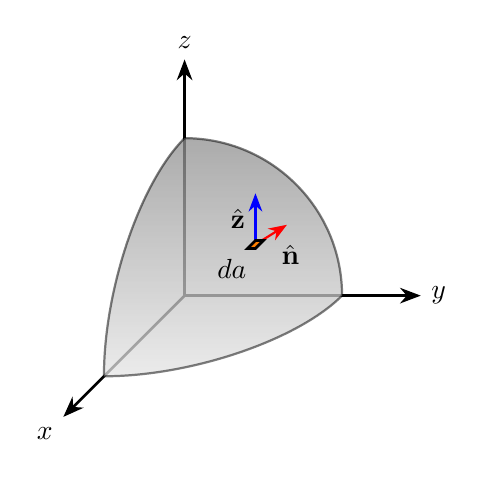
\begin{tikzpicture}[line width=1pt,line cap = round,>={Stealth},every edge/.style={draw=black,very thick}]
        \draw[->] (0,0,0) -- (3,0,0) node[right] {$y$};
        \draw[->] (0,0,0) -- (0,3,0) node[above] {$z$};
        \draw[->] (0,0,0) -- (0,0,4) node[below left] {$x$};
        \shade[fill=gray!60!white,opacity=0.5,draw=black,thick] (2,0) arc (0:90:2) {[x={(0,0,1.33)}] arc (90:0:2)} {[y={(0,0,1.33)}] arc (90:0:2)};
        \draw[->,thick,draw=blue] (0.9,0.65) -- node [left] {$\hat{\mathbf{z}}$} (0.9,1.3);
        \draw[->,thick,draw=red] (0.9,0.65) -- node [below right] {$\hat{\mathbf{n}}$} (1.3,0.9);
        \draw[fill=orange] (0.8,0.6) -- (0.9,0.6) -- (1,0.7) -- (0.9,0.7) --cycle;
        \node at (0.6,0.6) [below] {$da$};
    \end{tikzpicture}
        \caption{Geometry for Wangsness 1-12}
        \label{fig:EMAG_1_geometry_for_wangsness_1_12}
  \end{subfigure}
    \caption{Figures for Problems \ref{problem:EMAG_1_Wangsness_1_11} and \ref{problem:EMAG_1_wangsness_1_12}, Respectively.}
    \label{fig:EMAG_1_figures_for_wangsness_1_11_and_1_12}
\end{figure}
\begin{problem}[Wangsness 1-12]
\label{problem:EMAG_1_wangsness_1_12}
Find the surface integral of $\mathbf{r}$ and the volume integral of the volume integral of $\nabla \cdot \mathbf{r}$ for a sphere of radius $a_{0}$ centered at the origin.
\end{problem}
\begin{proof}[Solution]
The \textit{surface integral} of $\mathbf{A}$ over a closed surface $\partial\Sigma$ is defined as:
\begin{equation*}
    \oiint_{\partial\Sigma} \mathbf{A}\cdot\boldsymbol{da} = \oiint_{\partial\Sigma}\mathbf{A}\cdot\hat{\boldsymbol{n}}da
\end{equation*}
Where $\hat{\mathbf{n}}$ is the unit normal to the surface $\partial\Sigma$. For a sphere, we have:
\begin{equation*}
    \hat{\mathbf{n}}=\frac{\nabla(u)}{\norm{\nabla(u)}}=\frac{2x\hat{\mathbf{x}}+2y\hat{\mathbf{y}}+2z\hat{\mathbf{z}}}{\sqrt{4x^{2}+4y^{2}+4z^{2}}}= \frac{x\hat{\mathbf{x}}+\hat{\mathbf{y}}+z\hat{\mathbf{z}}}{\sqrt{x^2+y^2+z^2}}
\end{equation*}
Thus, we have:
\begin{equation*}
    \oiint_{\partial\Sigma}\mathbf{r}\cdot\hat{\mathbf{n}}da=\oiint_{\partial\Sigma}\bigg(x\hat{\mathbf{x}}+y\hat{\mathbf{y}}+z\hat{\mathbf{z}}\bigg)\cdot \bigg(\frac{x\hat{\mathbf{x}}+y\hat{\mathbf{y}}+z\hat{\mathbf{z}}}{\sqrt{x^{2}+y^{2}+z^{2}}}\bigg)da=\oiint_{\partial\Sigma}\sqrt{x^{2}+y^{2}+z^{2}}da
\end{equation*}
But recall that $x^{2}+y^{2}+z^{2} = a_{0}^{2}$, so we have:
\begin{equation*}
    \oiint_{\partial\Sigma}\mathbf{r}\cdot\boldsymbol{da} = a_{0}\oiint_{\partial\Sigma}da\\
\end{equation*}
But $\oiint_{\Sigma}da$ is just the surface area of $\Sigma$. And the surface area of the sphere is $4\pi a_{0}^{2}$. So:
\begin{equation*}
    \oiint_{\partial\Sigma}\mathbf{r}\cdot \boldsymbol{da} = 4\pi a_{0}^{3}
\end{equation*}
Using spherical coordinates is much easier.
\begin{equation*}
    \oiint_{\partial\Sigma}\mathbf{r}\cdot\boldsymbol{da}=\int_{0}^{2\pi}\int_{0}^{\pi}a_{0}\hat{\mathbf{r}}\cdot\hat{\mathbf{r}}a_{0}^{2}\sin(\theta)d\theta d\varphi= \int_{0}^{2\pi}\int_{0}^{\pi}a_{0}^{3}\sin(\theta)d\theta d\varphi=2\pi a_{0}^{3} \int_{0}^{\pi}\sin(\theta)d\theta=4\pi a_{0}^{3}
\end{equation*}
To compute the \textit{volume integral} of $\nabla \cdot \mathbf{r}$ within $\Sigma$, we must first compute $\nabla\cdot \mathbf{r}$:
\begin{equation*}
    \nabla\cdot\mathbf{r}=\frac{\partial x}{\partial x}+\frac{\partial y}{\partial y}+\frac{\partial z}{\partial z}=3
\end{equation*}
So, we have:
\begin{equation*}
    \iiint_{\Sigma}\nabla\cdot\mathbf{r}d\tau=\iiint_{\Sigma}3d\tau=3\iiint_{\Sigma}d\tau=3\frac{4}{3}\pi a_{0}^{3}=4\pi a_{0}^{3}
\end{equation*}
\end{proof}
\begin{problem}[Wangsness 1-13]
\label{problem:EMAG_1_wangsness_1_13}
Given the vector field $\mathbf{A} = xy\hat{\mathbf{x}}+yz\hat{\mathbf{y}}+xz\hat{\mathbf{z}}$, evaluate the flux of $\mathbf{A}$ through the surces of a parallelepiped of sides $a,b,c$ shown in figure \subref{fig:EMAG_1_wangsness_1_13_region_of_integration}. Compute $\int \nabla \cdot \mathbf{A}d\tau$ over the volume of the same parallelepiped.
\end{problem}
\begin{proof}[Solution]
There are six sides we must integrate over. Given $\mathbf{A} = xy\hat{\mathbf{x}}+yz\hat{\mathbf{y}}+xz\hat{\mathbf{z}}$, we have:
\begin{align*}
    \oiint_{\partial \Sigma}\mathbf{A}\cdot \boldsymbol{da} &= \oiint_{\partial \Sigma} (xydydz + yzdxdz+xzdxdz)\\
    &=\underset{\textrm{Front}}{\iint}xydydz-\underset{\textrm{Back}}{\iint}xydydz+\underset{\textrm{Right}}{\iint}yzdxdz-\underset{\textrm{Left}}{\iint}yzdxdz+\underset{\textrm{Top}}{\iint}xzdxdy-\underset{\textrm{Bottom}}{\iint}xzdxdy\\
    &=\int_{0}^{c}\int_{0}^{b}(a)ydydz+\int_{0}^{c}\int_{0}^{a}(b)zdxdz+\int_{0}^{b}\int_{0}^{a}x(c)dxdy=\frac{abc}{2}(a+b+c)
\end{align*}
To compute $\iiint_{V}\nabla\cdot\mathbf{A}d\tau$, we have: $\nabla\cdot\mathbf{A}=\frac{\partial(xy)}{\partial x}+\frac{\partial(yz)}{\partial y}+\frac{\partial(xz)}{\partial z}=x+y+z$. Thus:
\begin{align*}
    \iiint_{\Sigma}\nabla\cdot\mathbf{A}d\tau &=\iiint_{\Sigma}(x+y+z)d\tau=\int_{0}^{c}\int_{0}^{b}\int_{0}^{a}(x+y+z)dxdydz\\
    &=\int_{0}^{c}\int_{0}^{b}\int_{0}^{a}xdxdydz+\int_{0}^{c}\int_{0}^{b}\int_{0}^{a}ydxdydz+\int_{0}^{c}\int_{0}^{b}\int_{0}^{a}zdxdydz\\
    &=\frac{a^{2}bc}{2}+\frac{ab^{2}c}{2}+\frac{abc^{2}}{2}=\frac{abc}{2}(a+b+c)
\end{align*}
\end{proof}
\begin{figure}[H]
    \vspace{-4ex}
    \centering
    \begin{subfigure}[b]{0.49\textwidth}
    \resizebox{\linewidth}{!}{
    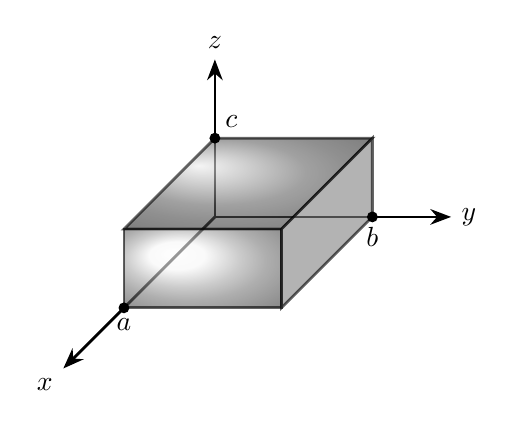
\begin{tikzpicture}[line width=1pt,line cap = round,>={Stealth},every edge/.style={draw=black,very thick}]
        \draw[->] (0,0,0) -- (3,0,0) node[right] {$y$};
        \draw[->] (0,0,0) -- (0,2,0) node[above] {$z$};
        \draw[->] (0,0,0) -- (0,0,5) node[below left] {$x$};
        \draw[ball color=gray!10!white,opacity=0.6] (0,0,3) -- (2,0,3) -- (2,1,3) -- (0,1,3) -- cycle;
        \draw[ball color = gray!90!white,opacity=0.6] (0,1,3) -- (0,1,0) -- (2,1,0) -- (2,1,3) -- cycle;
        \draw[fill=gray,opacity=0.6] (2,1,3) -- (2,0,3) -- (2,0,0) -- (2,1,0) --cycle;
        \filldraw[fill=black] (0,0,3) circle (0.05) node [below] {$a$};
        \filldraw[fill=black] (0,1,0) circle (0.05) node [above right] {$c$};
        \filldraw[fill=black] (2,0,0) circle (0.05) node [below] {$b$};
    \end{tikzpicture}}
    \caption{Wangsness 1-13}
    \label{fig:EMAG_1_wangsness_1_13_region_of_integration}
    \end{subfigure}
    \begin{subfigure}[b]{0.49\textwidth}
        \centering
        \begin{tikzpicture}[>=triangle 45,]
        \begin{axis}[width=\linewidth,axis lines=center,axis lines=middle,
            xlabel = $x$,xmin=-0.3,xmax=4,xtick distance=3,
            ylabel = $y$,ymin=-0.3,ymax=5,ytick distance=4,]
            \addplot[->,mark=none,line width=0.2mm,samples=5,domain=0:1.7,draw=blue] (x,0);
            \addplot[-,mark=none,line width=0.2mm,samples=5,domain=1.4:3,draw=blue] (x,0);
            \addplot[->,mark=none,line width=0.2mm,samples=5,domain=0:2.2,draw=blue] (3,x);
            \addplot[-,mark=none,line width=0.2mm,samples=5,domain=1.9:4,draw=blue] (3,x);
            \addplot[-,mark=none,line width=0.2mm,samples=5,domain=0:1.4,draw=blue] (x,4);
            \addplot[<-,mark=none,line width=0.2mm,samples=5,domain=1.3:3,draw=blue] (x,4);
            \addplot[-,mark=none,line width=0.2mm,samples=5,domain=0:2,draw=blue] (0,x);
            \addplot[<-,mark=none,line width=0.2mm,samples=5,domain=1.8:4,draw=blue] (0,x);
        \end{axis}
    \end{tikzpicture}
        \caption{Wangsness 1-14}
        \label{fig:EMAG_1_wangsness_1_14}
    \end{subfigure}
    \caption{Figures for problems \ref{problem:EMAG_1_wangsness_1_13} and \ref{problem:EMAG_1_wangsness_1_14}, Respectively.}
\end{figure}
\begin{problem}[Wangsness 1-14]
\label{problem:EMAG_1_wangsness_1_14}
Given $\mathbf{A} = -y\hat{\mathbf{x}}+x\hat{\mathbf{y}}$, calculate the line integral $\oint \mathbf{A}\cdot \mathbf{ds}$ over the closed path in the $xy$ plane shown in figure \subref{fig:EMAG_1_wangsness_1_14}.
\end{problem}
\begin{proof}[Solution]
Given $\mathbf{A} = -y\hat{\mathbf{x}}+x\hat{\mathbf{y}}$, we have:
\begin{align*}
    \oint_{\partial S}\mathbf{A}\cdot\boldsymbol{d\ell}&=\oint_{\partial S}\big(-y\hat{\mathbf{x}}+x\hat{\mathbf{y}}\big)\cdot\big(dx\hat{\mathbf{x}}+dy\hat{\mathbf{y}}\big)\\
    &=\underbrace{\int_{0}^{3}(-ydx+xdy)}_{y=0,\ dy=0}+\underbrace{\int_{0}^{4}(-ydx+xdy)}_{x=3,\ dx=0}+\underbrace{\int_{3}^{0}(-ydx+xdy)}_{y =4,\ dy=0}+\underbrace{\int_{4}^{0}(-ydx+xdy)}_{x=0,\ dx=0}\\
    &=0+12+12+0=24
\end{align*}
Next, we compute $\iint(\nabla\times\mathbf{A})\cdot\boldsymbol{da}$. We have $\nabla\times\mathbf{A}=2\hat{\mathbf{z}}$. Thus:
\begin{equation*}
    \iint_{S}\big(\nabla\times\mathbf{A}\big)\cdot\boldsymbol{da}=\iint_{S}\big(2\hat{\mathbf{z}}\big)\cdot \big(dydz\hat{\mathbf{x}}+dxdz\hat{\mathbf{y}}+dxdy\hat{\mathbf{z}}\big)=\int_{0}^{4}\int_{0}^{3}2dydx=24
\end{equation*}
\end{proof}
\begin{problem}[Wangsness 1-15]
\label{problem:EMAG_1_wangsness_1_15}
Given $\mathbf{A} = x^{2}y\hat{\mathbf{x}}+xy^{2}\hat{\mathbf{y}}+a^{3}e^{-\beta y}\cos(\alpha x)\hat{\mathbf{z}}$, compute $\oint \mathbf{A}\cdot \boldsymbol{d\ell}$ along the path in figure \ref{fig:EMAG_1_wangsness_1_15}. Compute $\iint (\nabla \times \mathbf{A})\cdot \boldsymbol{da}$ over the same region.
\end{problem}
\begin{figure}[H]
        \centering
        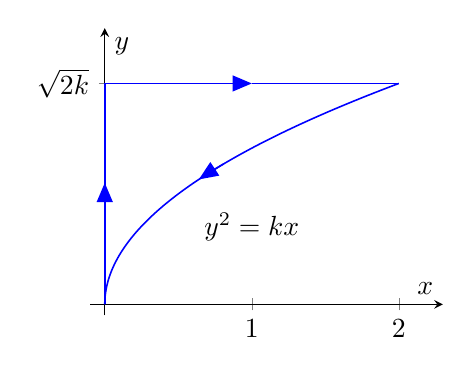
\begin{tikzpicture}[>=triangle 45,]
        \begin{axis}[width=0.5\linewidth,axis lines=center,axis lines=middle,
            xlabel = $x$,xmin=-0.1,xmax=2.3,xtick distance=1,
            ylabel = $y$,ymin=-0.1,ymax=2.5,ytick distance=2,
            yticklabel={$\sqrt{\pgfmathprintnumber{\tick}k}$}]
            \addplot[-,mark=none,line width=0.2mm,samples=100,domain=0:0.9,draw=blue] (x*x,1.4142*x);
            \addplot[<-,mark=none,line width=0.2mm,samples=100,domain=0.8:1.414214,draw=blue] (x*x,1.4142*x);
            \addplot[-,mark=none,line width=0.2mm,samples=10,domain=1:2,draw=blue] (0,x);
            \addplot[->,mark=none,line width=0.2mm,samples=10,domain=0:1.1,draw=blue] (0,x);
            \addplot[->,mark=none,line width=0.2mm,samples=10,domain=0:1,draw=blue] (x,2);
            \addplot[-,mark=none,line width=0.2mm,samples=10,domain=1:2,draw=blue] (x,2);
            \node at (axis cs:1,0.7) {$y^2=kx$};
        \end{axis}
    \end{tikzpicture}
    \caption{Figure for Problem \ref{problem:EMAG_1_wangsness_1_15}}
    \label{fig:EMAG_1_wangsness_1_15}
\end{figure}
\begin{proof}[Solution]
Along the entire contour, we have $z=0$ and $dz=0$. Thus, we have:
\begin{equation*}
    \oint_{\partial S}\mathbf{A}\cdot\boldsymbol{d\ell}=\oint_{\partial S}\big(x^{2}y\hat{\mathbf{x}}+xy^{2}\hat{\mathbf{y}}+a^{3}e^{\beta y}\cos(\alpha x)\hat{\mathbf{z}}\big)\cdot\big(dx\hat{\mathbf{x}}+dy\hat{\mathbf{y}}\big)=\oint_{\partial S}\big(x^{2}ydx+xy^{2}dy\big)
\end{equation*}
Along the first path, we have $x=0$ and $dx=0$. Along the second path, we have $y=\sqrt{2k}, dy=0$. Along the third path we have $y^2=kx$, and thus $dx = \frac{2ydy}{k}$. Thus:
\begin{align*}
    \oint_{\partial S}\mathbf{A}\cdot\boldsymbol{d\ell}&=\int_{C_{1}}\mathbf{A}\cdot\boldsymbol{d\ell}+\int_{C_{2}}\mathbf{A}\cdot\boldsymbol{d\ell}+\int_{C_{3}}\mathbf{A}\cdot\boldsymbol{d\ell}\\
    &=\int_{0}^{\sqrt{2k}}(0)y^{2}dy+\int_{0}^{2}x^{2}\sqrt{2k}dx+\int_{\sqrt{2k}}^{0}\big(\frac{y^{4}}{k^2}y\frac{2y}{k}dy+\frac{y^{2}}{k}y^{2}dy\big)\\
    &=\frac{8}{3}\sqrt{2k}+\int_{\sqrt{2k}}^{0}\big(2\frac{y^{6}}{k^{3}}+\frac{y^{4}}{k}\big)dy=\frac{8}{3}\sqrt{2k}-\frac{2}{7}\sqrt{2k}-\frac{4k\sqrt{2k}}{5}=\sqrt{2k}\big(\frac{8}{21}-\frac{4}{5}k\big)
\end{align*}
Next we compute $\iint (\nabla \times \mathbf{A})\cdot \boldsymbol{da}$. Note that $\boldsymbol{da} = \hat{\mathbf{z}}dxdy$. The $\hat{\mathbf{z}}$ component for $\nabla \times \mathbf{A}$ is $(y^{2}-x^{2})\hat{\mathbf{z}}$. We have:
\begin{align*}
    \iint_{\Sigma}\big(\nabla\times\mathbf{A}\big)\cdot\boldsymbol{da}&=\int_{0}^{2}\int_{\sqrt{kx}}^{\sqrt{2k}} \big(x^{2}-y^{2}\big)dydx=\int_{0}^{2}\bigg[x^{2}y-\frac{y^{3}}{3}\bigg]_{\sqrt{kx}}^{\sqrt{2k}}dx\\
    &= \int_{0}^{2}\bigg[\bigg(x^{2}\sqrt{2k} - \frac{2k\sqrt{2k}}{3}\bigg) - \bigg(x^{2}\sqrt{kx} - \frac{kx\sqrt{kx}}{3}\bigg)\bigg]dx\\
    &= \sqrt{2k}\int_{0}^{2}x^2 dx - \frac{2k}{3}\sqrt{2k}\int_{0}^{2}dx - \sqrt{k}\int_{0}^{2}x^{\frac{5}{2}}dx + \frac{k\sqrt{k}}{3}\int_{0}^{2}x^{\frac{3}{2}}dx\\
    &=\frac{8}{3}\sqrt{2k}-\frac{4k}{3}\sqrt{2k}-\frac{16}{7}\sqrt{2k}+\frac{8k}{15}\sqrt{2k}=\frac{8}{21}\sqrt{2k}-\frac{4}{5}k\sqrt{2k}=\sqrt{2k}\big(\frac{8}{21}-\frac{4k}{5}\big)
\end{align*}
\end{proof}
\subsection{Homework III}
Wangsness Chapter 1 - Problems: 19, 20, 21, 22, 23, 24, 26
\begin{problem}[Wangsness 1-19]
Let $\mathbf{A} = a\hat{\boldsymbol{\uprho}}+b\hat{\boldsymbol{\upvarphi}}+c\hat{\mathbf{z}}$, where $a,b,c$ are constants.Is $\mathbf{A}$ a constant vector? Find $\nabla\cdot \mathbf{A}$ and $\nabla\times \mathbf{A}$. Find the rectangular and spherical components of $\mathbf{A}$, expressing in terms of $x,y,z$ and $r,\theta,\varphi$, respectively.
\end{problem}
\begin{proof}[Solution]
If $a$ or $b$ are non-zero, then $\mathbf{A}$ is not a constant, for $\hat{\boldsymbol{\uprho}}$ and $\hat{\boldsymbol{\upvarphi}}$ are functions of $\varphi$. To compute $\nabla \cdot \mathbf{A}$, we use $\nabla$ in cylindrical coordinates and do:
\begin{equation*}
    \nabla\cdot\mathbf{A}=\frac{\partial A_{\rho}}{\partial \rho}+\frac{A_{\rho}}{\rho}+\frac{1}{\rho}\frac{\partial A_{\phi}}{\partial\varphi}+\frac{\partial A_{z}}{\partial z}=\frac{\partial a}{\partial\rho}+\frac{a}{\rho}+\frac{1}{\rho}\frac{\partial b}{\partial\varphi}+\frac{\partial A_{z}}{\partial z}=\frac{a}{\rho}
\end{equation*}
For $\nabla\times\mathbf{A}$, we again use cylindrical coordinates and do:
\begin{align*}
    \nabla \times \mathbf{A} = \begin{vmatrix} \frac{1}{\rho}\hat{\boldsymbol{\uprho}}& \hat{\boldsymbol{\upvarphi}} & \frac{1}{\rho}\hat{\mathbf{z}} \\ \frac{\partial}{\partial \rho} & \frac{\partial}{\partial \varphi} & \frac{\partial}{\partial z} \\ A_{\rho} &  \rho A_{\varphi} & A_z \end{vmatrix}&= \frac{\hat{\boldsymbol{\uprho}}}{\rho}\bigg(\frac{\partial A_{z}}{\partial \varphi} - \frac{\partial (\rho A_{\varphi})}{\partial z}\bigg) + \hat{\boldsymbol{\upvarphi}}\bigg(\frac{\partial A_{\rho}}{\partial z} - \frac{\partial A_{z}}{\partial \rho}\bigg) + \frac{\hat{\mathbf{z}}}{\rho}\bigg(\frac{\partial (\rho A_{\varphi})}{\partial \rho} - \frac{\partial A_{\rho}}{\partial \varphi}\bigg)\\
    &=\hat{\boldsymbol{\uprho}}\bigg(\frac{1}{\rho}\frac{\partial A_{z}}{\partial\varphi}-\frac{\partial A_{\varphi}}{\partial z}\bigg)+\hat{\boldsymbol{\upvarphi}}\bigg(\frac{\partial A_{\rho}}{\partial z}-\frac{\partial A_{z}}{\partial \rho}\bigg)+\hat{\mathbf{z}}\bigg(\frac{1}{\rho}\frac{\partial (\rho A_{\varphi})}{\partial\rho}-\frac{1}{\rho}\frac{\partial A_{\rho}}{\partial \varphi}\bigg)\\
    &=\hat{\boldsymbol{\uprho}}(0-0)+\hat{\boldsymbol{\upvarphi}}(0-0)+\hat{\mathbf{z}}(\frac{A_\phi}{\rho} +0-0)=\frac{b}{\rho}\hat{\mathbf{z}}
\end{align*}
Rectangular coordinates of $\mathbf{A}$:
\begin{align*}
    \mathbf{A} &= a(\cos(\phi)\hat{\mathbf{x}}+\sin(\phi)\hat{\mathbf{y}})+b(-\sin(\phi)\hat{\mathbf{x}}+\cos(\phi)\hat{\mathbf{y}})+c\hat{\mathbf{z}}\\
    &= a\bigg(\frac{x\hat{\mathbf{x}}+y\hat{\mathbf{y}}}{\sqrt{x^2+y^2}}\bigg)+b\bigg(\frac{-y\hat{\mathbf{x}}+x\hat{\mathbf{y}}}{\sqrt{x^2+y^2}}\bigg)+c\hat{\mathbf{z}}=\frac{ax-by}{\sqrt{x^2+y^2}}\hat{\mathbf{x}}+\frac{ay+bx}{\sqrt{x^2+y^2}}\hat{\mathbf{y}}+c\hat{\mathbf{z}}
\end{align*}
For spherical coordinates, first note that:
\begin{align*}
    \rho^{2}&=x^{2}+y^{2}=x^2+y^2+z^2-z^2=r^2-z^2=r^{2}-r^{2}\cos(\theta)^2=r^2\big(1-\cos(\theta)^2\big)=r^2\sin^2(\theta)
\end{align*}
We can use the rectangular coordinates previously obtained to convert to spherical coordinates:
\begin{align*}
    \hat{\mathbf{A}} &= \bigg(\frac{ar\cos(\varphi)\sin(\theta)-br\sin(\varphi)\cos(\theta)}{r\sin(\theta)}\bigg)\big(\sin(\theta)\cos(\varphi)\hat{\mathbf{r}}+\cos(\theta)\sin(\theta)\hat{\boldsymbol{\uptheta}}-\sin(\varphi)\hat{\boldsymbol{\upvarphi}}\big)\\
    &+\bigg(\frac{ar\sin(\varphi)\sin(\theta)+br\cos(\varphi)\sin(\theta)}{r\sin(\theta)}\bigg)\big(\sin(\theta)\sin(\varphi)\hat{\mathbf{r}}+\cos(\theta)\sin(\varphi)\hat{\boldsymbol{\uptheta}}+\cos(\varphi)\hat{\boldsymbol{\upvarphi}}\big)\\
    &+c\big(\cos(\theta)\hat{\mathbf{r}}-\sin(\theta)\hat{\boldsymbol{\uptheta}}\big)\\
    &= \big(a\sin(\theta)+c\cos(\theta)\big)\hat{\mathbf{r}}+\big(a\cos(\theta)-c\sin(\theta)\big)\hat{\boldsymbol{\uptheta}}+b\hat{\boldsymbol{\upvarphi}}
\end{align*}
\end{proof}
\begin{problem}[Wangsness 1-20]
Let $\mathbf{A} = a\hat{\mathbf{r}} + b\hat{\boldsymbol{\uptheta}}+c\hat{\boldsymbol{\upvarphi}}$. Is $\mathbf{A}$ a constant vector? Find $\nabla\cdot \mathbf{A}$ and $\nabla\times \mathbf{A}$. Find the rectangular and cylindrical components of $\mathbf{A}$, expressing in terms of $x,y,z$ and $\rho,\varphi,z$, respectively.
\end{problem}
\begin{proof}[Solution]
If $a$ or $b$ or $c$ are non-zero, then $\mathbf{A}$ is not a constant vector, for $\hat{\mathbf{r}}$, $\hat{\boldsymbol{\uptheta}}$, and $\hat{\boldsymbol{\upvarphi}}$ are functions of $r,\theta,\varphi$. To compute $\nabla \cdot \mathbf{A}$, we use spherical coordinates and do:
\begin{equation*}
    \nabla\cdot\mathbf{A}=\frac{1}{r^{2}}\frac{\partial (r^{2}A_{r})}{\partial r}+\frac{1}{r\sin(\theta)}\frac{\partial(\sin(\theta)A_{\theta})}{\partial \theta}+\frac{1}{r\sin(\theta)}\frac{\partial A_{\varphi}}{\partial\varphi}=\frac{2a}{r}+\frac{b\cos(\theta)}{r\sin(\theta)}
\end{equation*}
For $\nabla \times \mathbf{A}$:
\begin{align*}
    \nabla \times \mathbf{A} &= \begin{vmatrix} \frac{1}{r^{2}\sin(\theta)}\hat{\mathbf{r}} & \frac{1}{r\sin(\theta)}\hat{\boldsymbol{\uptheta}} & \frac{1}{r}\hat{\boldsymbol{\upvarphi}}\\ \frac{\partial}{\partial r} & \frac{\partial}{\partial \theta} & \frac{\partial}{\partial \varphi}\\ A_{r} & rA_{\theta} & r\sin(\theta)A_{\varphi} \end{vmatrix}\\
    &= \frac{\hat{\mathbf{r}}}{r\sin(\theta)}\bigg(\frac{\partial (\sin(\theta)A_{\varphi})}{\partial \theta} - \frac{\partial A_{\theta}}{\partial \varphi}\bigg) + \frac{\hat{\boldsymbol{\uptheta}}}{r}\bigg(\frac{1}{\sin(\theta)}\frac{\partial A_{r}}{\partial \varphi} - \frac{\partial (rA_{\varphi})}{\partial r}\bigg)+\frac{\hat{\boldsymbol{\upvarphi}}}{r}\bigg(\frac{\partial (rA_{\theta})}{\partial r} - \frac{\partial A_{r}}{\partial \theta}\bigg)\\
    &= \frac{\cos(\theta)}{r\sin(\theta)}\hat{\mathbf{r}}-\frac{c}{r}\hat{\boldsymbol{\uptheta}}+\frac{b}{r}\hat{\boldsymbol{\upvarphi}}
\end{align*}
In rectangular coordinates, we have:
\begin{align*}
    \mathbf{A}  &= a\big(\sin(\theta)\cos(\varphi)\hat{\mathbf{x}}+\sin(\theta)\sin(\varphi)\hat{\mathbf{y}}+\cos(\theta)\hat{\mathbf{z}}\big)\\
                &+ b\big(\cos(\theta)\cos(\varphi)\hat{\mathbf{x}} + \cos(\theta)\sin(\varphi)\hat{\mathbf{y}}-\sin(\theta)\hat{\mathbf{z}}\big)\\
                &+ c\big(-\sin(\varphi)\hat{\mathbf{x}} + \cos(\varphi)\hat{\mathbf{y}}\big)\\
                &= \frac{a}{\sqrt{x^{2}+y^{2}+z^{2}}}\bigg(x\hat{\mathbf{x}} + y\hat{\mathbf{y}}+z\hat{\mathbf{z}}\bigg)\\
                &+ \frac{b}{\sqrt{x^{2}+y^{2}+z^{2}}}\bigg(\frac{xz}{\sqrt{x^2+y^2}}\hat{\mathbf{x}} + \frac{yz}{\sqrt{x^{2}+y^{2}}}\hat{\mathbf{y}} - \sqrt{x^2+y^2}\hat{\mathbf{z}}\bigg)\\
                &+ -\frac{y}{\sqrt{x^2+y^2}}\hat{\mathbf{x}} + \frac{x}{\sqrt{x^{2}+y^{2}}}\hat{\mathbf{y}}\\
                &= \bigg(\frac{ax}{\sqrt{x^{2}+y^{2}+z^{2}}}+\frac{bxz}{\sqrt{x^2+y^2}\sqrt{x^{2}+y^{2}+z^{2}}} - \frac{y}{\sqrt{x^2+y^2}}\bigg)\hat{\mathbf{x}}\\
                &+\bigg(\frac{ay}{\sqrt{x^{2}+y^{2}+z^{2}}}+\frac{byz}{\sqrt{x^2+y^2}\sqrt{x^{2}+y^{2}+z^{2}}} + \frac{x}{\sqrt{x^{2}+y^{2}}}\bigg)\hat{\mathbf{y}}\\
                &+ \frac{az}{\sqrt{x^{2}+y^{2}+z^{2}}} - \frac{b\sqrt{x^{2}+y^{2}}}{\sqrt{x^{2}+y^{2}+z^{2}}}\bigg)\hat{\mathbf{z}}
\end{align*}
We can then use this to convert to cylindrical, recalling that $r^{2} = \rho^{2}+z^{2}$:
\begin{equation*}
    \mathbf{A} = \bigg(\frac{a\rho+bz}{\sqrt{\rho^2+z^2}}\bigg)\hat{\boldsymbol{\uprho}}+c\hat{\boldsymbol{\upvarphi}}+\bigg(\frac{az-b\rho}{\sqrt{\rho^2+z^2}}\bigg)\hat{\mathbf{z}}
\end{equation*}
\end{proof}
\begin{problem}[Wangsness 1-21]
Find $\nabla\cdot\mathbf{r}$ for the position vector $\mathbf{r}$ expressed in rectangular, cylindrical, and spherical coordinates.
\end{problem}
\begin{proof}[Solution]
In rectangular coordinates we have $\mathbf{r} = x\hat{\mathbf{x}} + y\hat{\mathbf{y}} + z\hat{\mathbf{z}}$. So:
\begin{equation*}
    \nabla\cdot\mathbf{r}=\frac{\partial x}{\partial x}+\frac{\partial y}{\partial y}+\frac{\partial z}{\partial z}=1+1+1= 3
\end{equation*}
In cylindrical coordinates, $\mathbf{r} = \rho\hat{\boldsymbol{\uprho}} + z\hat{\mathbf{z}}$, So:
\begin{equation*}
    \nabla\cdot\mathbf{r}=\frac{1}{\rho}\frac{\partial}{\partial \rho}\big(\rho^2\big)+\frac{1}{\rho}\frac{\partial}{\partial\phi}\big(0\big)+\frac{\partial z}{\partial z}=2+0+1=3
\end{equation*}
In spherical coordinates we have:
\begin{equation*}
    \nabla\cdot\mathbf{r}=\frac{1}{r^2}\frac{\partial}{\partial r}\big(r^2 r\big)=3
\end{equation*}
\end{proof}
\begin{problem}[Wangsness 1-22]
Let $\mathbf{A} = a\rho\hat{\boldsymbol{\uprho}} + b\hat{\boldsymbol{\upvarphi}}+cz\hat{\mathbf{z}}$, where $a,b,c$ are constants. Find $\oiint \mathbf{A}\cdot \boldsymbol{da}$ over the surface of a right circular cylinder of length $L$ and radius $\rho_{0}$ whose axis is along the positive $z$ axis and the origin is the center of the lower circular face (See Fig.~\subref{fig:EMAG_1_wangsness_1_22}). Find $\iiint \nabla \cdot \mathbf{A}d\tau$ over the volume of the cylinder.
\end{problem}
\begin{proof}[Solution]
We have that:
\begin{equation*}
    \oint \mathbf{A}\cdot \boldsymbol{da} = \int_{Top} \mathbf{A}\cdot \boldsymbol{da}+\int_{Cylinder} \mathbf{A}\cdot \boldsymbol{da} + \int_{Bottom} \mathbf{A}\cdot \boldsymbol{da}
\end{equation*}
On the cylindrical surface, $da = \rho_0 d\phi dz$, so the integral is:
\begin{align*}
    \int_{0}^{L}\int_{0}^{2\pi}(a\rho_0\hat{\boldsymbol{\uprho}}+b\hat{\boldsymbol{\upvarphi}}+cz\hat{\mathbf{z}})\cdot \rho_0 \hat{\boldsymbol{\uprho}}d\varphi dz &= \int_{0}^{L}\int_{0}^{2\pi}a\rho_0^2 d\phi dz\\
    &= a\rho_0^2(2\pi)L    
\end{align*}
For the top and bottom, $da = \pm \rho d\rho d\phi \hat{\mathbf{z}}$, respectively. On the bottom surface $z=0$ and thus the integral is zero. On the top we get:
\begin{equation*}
\int_{0}^{2\pi}\int_{0}^{\rho_0}cL\rho d\rho d\phi = \pi cL \rho_0^2
\end{equation*}
%
Thus:
%
\begin{equation*}
\oiint \mathbf{A}\cdot \boldsymbol{da} = \pi L \rho_0^2(2a+c)
\end{equation*}
%
Computing the divergence, we get $\nabla \cdot \mathbf{A} = 2a+c$. Therefore:
\begin{equation*}
    \iiint_C \nabla \cdot \mathbf{A} d\tau = (2a+c) V = \pi L \rho_0^2(2a+c)
\end{equation*}
\end{proof}
\begin{figure}[H]
    \centering
    \begin{subfigure}[b]{0.49\textwidth}
        \centering
        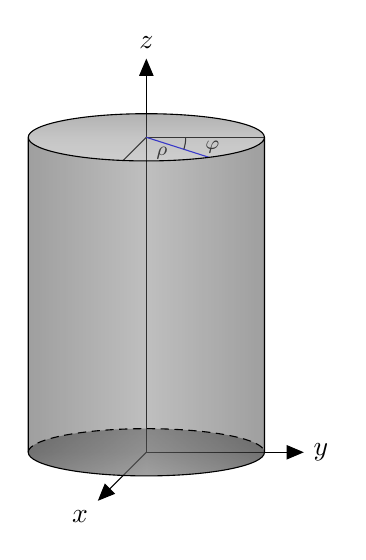
\begin{tikzpicture}[>=triangle 45,]
            \coordinate (x) at (0,0,1.6);
            \coordinate (y) at (2,0,0);
            \coordinate (z) at (0,5,0);
            \coordinate (xt) at (0,4,0.76);
            \coordinate (yt) at (1.5,4,0);
            \coordinate (zt) at (0,4,0);
            \coordinate (p) at (1.05,4,0.66);
            \draw[->] (0,0,0) -- (2,0,0) node[right] {$y$};
            \draw[->] (0,0,0) -- (0,5,0) node[above] {$z$};
            \draw[->] (0,0,0) -- (0,0,1.6) node[below left] {$x$};
            \draw[-] (0,4,0) -- (0,4,0.76) {};
            \draw[-] (0,4,0) -- (1.5,4,0) {};
            \draw[-,blue] (0,4,0) node [below=0.2cm,right,black] {\scriptsize{$\rho$}} -- (1.05,4,0.66) {};
            \pic [draw=black, -, "\scriptsize{${\varphi}$}", angle eccentricity=1.7, angle radius =0.5cm] {angle = p--zt--yt};
            \fill[top color=gray!50!black,bottom color=gray!10,middle color=gray,shading=axis,opacity=0.25] (0,0) circle (1.5cm and 0.3cm);
            \fill[left color=gray!50!black,right color=gray!50!black,middle color=gray!50,shading=axis,opacity=0.25] (1.5,0) -- (1.5,4) arc (360:180:1.5cm and 0.3cm) -- (-1.5,0) arc (180:360:1.5cm and 0.3cm);
            \fill[top color=gray!90!,bottom color=gray!2,middle color=gray!30,shading=axis,opacity=0.25] (0,4) circle (1.5cm and 0.3cm);
            \draw (-1.5,4) -- (-1.5,0) arc (180:360:1.5cm and 0.3cm) -- (1.5,4) ++ (-1.5,0) circle (1.5cm and 0.3cm);
            \draw[densely dashed] (-1.5,0) arc (180:0:1.5cm and 0.3cm);
        \end{tikzpicture}
        \caption{Wangsness 1-22}
        \label{fig:EMAG_1_wangsness_1_22}
    \end{subfigure}
    \begin{subfigure}[b]{0.49\textwidth}
        \centering
        \begin{tikzpicture}[>=triangle 45,]
        \begin{axis}[width=\textwidth,axis equal,axis lines=middle,
            xlabel = $x$,
            ylabel = $y$,
            xmin=-0.1,xmax=1.3,
            ymin=-0.1,ymax=1.3,
            axis lines=middle,
            xticklabel={$r_{0}$},
            yticklabel={$r_{0}$},
            xtick distance=1,
            ytick distance=1]
            \addplot[->,mark=none,line width=0.2mm,samples=3,domain=0:0.5,draw=blue] (x,0);
            \addplot[-,mark=none,line width=0.2mm,samples=3,domain=0.4:1,draw=blue] (x,0);
            \addplot[-,mark=none,line width=0.2mm,samples=50,domain=0:0.75,draw=blue,variable=\x] (\x,{sqrt(1-\x^2)});
            \addplot[<-,mark=none,line width=0.2mm,samples=50,domain=0.7:1,draw=blue,variable=\x] (\x,{sqrt(1-\x^2)});
            \addplot[-,mark=none,line width=0.2mm,samples=3,domain=0:0.6,draw=blue] (0,x);
            \addplot[<-,mark=none,line width=0.2mm,samples=3,domain=0.5:1,draw=blue] (0,x);
            \node at (axis cs:1,0.9) {$x^2+y^2=r_{0}^{2}$};
            \coordinate (a) at (axis cs:1,0);
            \coordinate (b) at (axis cs:0.8,0.6);
            \coordinate (o) at (axis cs:0,0);
            \draw[draw=red,thick] (axis cs:0,0) -- node [above] {$r_{0}$} (axis cs:4/5,3/5);
            \pic [draw=black, -, "$\theta$", angle eccentricity=1.5,angle radius = 0.6cm] {angle = a--o--b};
        \end{axis}
    \end{tikzpicture}
        \caption{Wangsness 1-23}
        \label{fig:EMAG_1_wangsness_1_23}
    \end{subfigure}
\end{figure}
\begin{problem}[Wangsness 1-23]
Let $\mathbf{A} = 4\hat{\mathbf{r}} + 3\hat{\boldsymbol{\uptheta}}-2\hat{\boldsymbol{\upvarphi}}$. Find the line integral around the closed path shown in Fig.~\subref{fig:EMAG_1_wangsness_1_23}. Find the surface integral of $\nabla \times \mathbf{A}$ over the enclosed area.
\end{problem}
\begin{proof}[Solution]
We have:
\begin{equation*}
    \oint_{\partial S}\mathbf{A}\cdot \boldsymbol{d\ell} = \sum_{i} \int_{\partial S_{i}} \mathbf{A}\cdot \boldsymbol{d\ell}
\end{equation*}
Along the first path $\varphi=0,\ \theta = \frac{\pi}{2}$, and $\boldsymbol{d\ell} = dr\hat{\mathbf{r}}$. The integral is then $4r_0$.
\begin{equation*}
    \int_{\partial S_{1}}\mathbf{A}\cdot\boldsymbol{d\ell}=\int_{0}^{r_{0}}(4\hat{\mathbf{r}}+3\hat{\boldsymbol{\uptheta}}-2\hat{\boldsymbol{\upvarphi}})\cdot (\hat{\mathbf{r}}dr)=4\int_{0}^{r_{0}}dr=4r_{0}
\end{equation*}
Along the second path $r=r_0$, $\theta = \frac{\pi}{2}$, and $\boldsymbol{d\ell} = r_0 d\varphi \hat{\boldsymbol{\upvarphi}}$.
\begin{equation*}
    \int_{\partial S_{2}}\mathbf{A}\cdot \hat{\boldsymbol{d\ell}}=\int_{0}^{\frac{\pi}{2}}(4\hat{\mathbf{r}}+3\hat{\boldsymbol{\uptheta}}-2\hat{\boldsymbol{\upvarphi}})\cdot(r_{0}d\varphi\hat{\boldsymbol{\upvarphi}})=-2\int_{0}^{\frac{\pi}{2}}r_{0}d\varphi=-\pi r_{0}
\end{equation*}
Along the final path, $\varphi = \frac{pi}{2}$, $\theta = \frac{\pi}{2}$, and $ \boldsymbol{d\ell} = dr \hat{\mathbf{r}}$.
\begin{equation*}
    \int_{\partial S_{3}}\mathbf{A}\cdot \boldsymbol{d\ell}=\int_{r_{0}}^{0}(4\hat{\mathbf{r}}+3\hat{\boldsymbol{\uptheta}}-2\hat{\boldsymbol{\upvarphi}})\cdot (\hat{\mathbf{r}}dr)=4\int_{r_{0}}^{0}dr=-4r_{0}
\end{equation*}
Therefore:
\begin{equation*}
    \oint_{\partial S}\mathbf{A}\cdot\boldsymbol{d\ell}=\sum_{i}\int_{\partial S_{i}}\mathbf{A}\cdot\boldsymbol{d\ell}=4r_{0}-\pi r_{0}-4r_{0}=-\pi r_{0}
\end{equation*}
The curl is: $\nabla\times\mathbf{A}=\frac{-2\cot(\theta)}{r}\hat{\mathbf{r}}+\frac{2}{r}\hat{\boldsymbol{\uptheta}}+\frac{3}{r}\hat{\boldsymbol{\upvarphi}}$. For the plane, $\boldsymbol{da}=\hat{\mathbf{z}}rdrd\varphi$ $\theta=\frac{\pi}{2}$. So:
\begin{align*}
    \iint \nabla \times \mathbf{A} \cdot \boldsymbol{da} &= \int_{0}^{\frac{\pi}{2}}\int_{0}^{r_{0}} \bigg(\frac{-2\cot(\theta)}{r}\hat{\mathbf{r}}+\frac{2}{r}\hat{\boldsymbol{\uptheta}}+\frac{3}{r}\hat{\boldsymbol{\upvarphi}}\bigg)\cdot \hat{\mathbf{z}} rdrd\varphi\\
    &= \int_{0}^{\frac{\pi}{2}}\int_{0}^{r_{0}}\bigg(-2\cot(\theta)\cos(\theta)-2\sin(\theta)\bigg)drd\varphi= -2\int_{0}^{\frac{\pi}{2}}\int_{0}^{r_{0}}drd\varphi=-\pi r_{0}
\end{align*}
\end{proof}
\begin{problem}[Wangsness 1-24]
Verify that $\nabla \times (u\mathbf{A}) = \nabla(u)\times \mathbf{A}+u(\nabla \times \mathbf{A})$
\end{problem}
\begin{proof}[Solution]
Let $\mathbf{A} = \langle A_x,A_y,A_z\rangle$ and $u = u(x,y,z)$. Using the product rule, we get:
\begin{align*}
    \nabla \times (u\mathbf{A}) &= \begin{vmatrix} \hat{\mathbf{x}} & \hat{\mathbf{y}} & \hat{\mathbf{z}} \\ \frac{\partial}{\partial x} & \frac{\partial}{\partial y} & \frac{\partial}{\partial z} \\ uA_x & uA_y & uA_z \end{vmatrix}\\
    &= \hat{\mathbf{x}}\big( \frac{\partial u}{\partial y} A_z + u \frac{\partial A_z}{\partial y}-\frac{\partial u}{\partial z}A_y -u \frac{\partial A_y}{\partial z}\big) + \hat{\mathbf{y}}\big(\frac{\partial u}{\partial z} A_x + u \frac{\partial A_x}{\partial z} - \frac{\partial u}{\partial x} A_z - u\frac{\partial A_z}{\partial x}\big)\\ &+ \hat{\mathbf{z}}\big(\frac{\partial u}{\partial x}A_y + u \frac{\partial A_y}{\partial x} - \frac{\partial u}{\partial y}A_x - u\frac{\partial A_x}{\partial y}\big)   
\end{align*}
%
But:
\begin{equation*}
    \nabla(u)\times \mathbf{A} = \hat{\mathbf{x}}\big(\frac{\partial u}{\partial y}A_z - \frac{\partial u}{\partial z}A_y\big) + \hat{\mathbf{y}}\big(\frac{\partial u}{\partial z}A_x - \frac{\partial u}{\partial x}A_z\big) + \hat{\mathbf{z}}\big(\frac{\partial u}{\partial x}A_y - \frac{\partial u}{\partial y}A_x\big)
\end{equation*}
%
and
%
\begin{equation*}
    u(\nabla \times \mathbf{A}) = \hat{\mathbf{x}}\big(u\frac{\partial A_z}{\partial y} - u\frac{\partial A_y}{\partial z}\big) + \hat{\mathbf{y}}\big(u\frac{\partial A_y}{\partial z} -u\frac{\partial A_z}{\partial y}A_x\big) + \hat{\mathbf{z}}\big(\frac{u\partial A_y}{\partial x}-u\frac{\partial A_x}{\partial y}\big)   
\end{equation*}
%
Summing these, we have $\nabla \times (u\mathbf{A}) =\nabla(u)\times \mathbf{A}+u\nabla \times \mathbf{A}$
\end{proof}
%
\begin{problem}[Wangsness 1-26]
Verify that $\oint_{S} u\boldsymbol{da}= \int_{V} \nabla(u)d\tau$ and $\oint_{S} \mathbf{A}\times \boldsymbol{da}= -\int_{V} \nabla \times \mathbf{A} d\tau$
\end{problem}
\begin{proof}[Solution]
Let $\mathbf{C}$ be an arbitrary constant vector. Then:
%
\begin{equation*}
    \mathbf{C}\cdot\bigg(\oiint_{S}u\boldsymbol{da} - \iiint_V \nabla(u)d\tau\bigg) = \oiint_{S} u \bigg(\mathbf{C}\cdot \boldsymbol{da}\bigg) - \iiint_{V} \bigg(\mathbf{C}\cdot \nabla(u)\bigg) d\tau    
\end{equation*}
%
But, as $\mathbf{C}$ is constant, $\nabla \cdot \mathbf{C} = 0$, and thus we have:
%
\begin{align*}
    \iiint_{V} \mathbf{C}\cdot \nabla(u) d\tau &= \iiint_{V} \nabla \cdot (u \mathbf{C}) d\tau - \iiint_{V} u \nabla \cdot \mathbf{C} d\tau\\
    &= \iiint_{V} \nabla(u\mathbf{C}) d\tau    
\end{align*}
But from the divergence theorem:
\begin{equation*}
    \iiint_{V}\nabla(u\mathbf{C}) d\tau = \oiint_{S}u\mathbf{C}\cdot \boldsymbol{da}
\end{equation*} Thus, $\mathbf{C}\cdot\big(\oint_{S}u \boldsymbol{da} - \int_{V} \nabla(u) d\tau \big) = 0$. As $\mathbf{C}$ is any arbitrary vector, $\oint_{S}u \boldsymbol{da} - \int_{V} \nabla(u) d\tau =0$ and thus $\oint_{S} u\boldsymbol{da}= \int_{V} \nabla(u)d\tau$. It is a simple exercise in vector geometry to show that if $\mathbf{A}\cdot \mathbf{C} = 0$ for all vectors $\mathbf{C}$, then $\mathbf{A} = \mathbf{0}$. In an analogous manner:
\begin{align*}
    \mathbf{C}\cdot\bigg(\oiint_{S}\mathbf{A}\times\boldsymbol{da}+\iiint_{V}\nabla\times\mathbf{A}d\tau\bigg)=0\Rightarrow\oiint_{S}\mathbf{A}\times \boldsymbol{da}=-\iiint_{V}\nabla\times\mathbf{A}d\tau
\end{align*}
\end{proof}
\subsection{Homework IV}
Wangsness Chapter 2: Problems 3, 7, 8\\
Wangsness Chapter 3: Problems 9, 10
\begin{problem}[Wangsness 2-3]
    Consider $8$ equal point charges $q$ located on the corners of a cube of length $a$, as in Fig.~\subref{fig:EMAG_1_Wangsness_2_3}. Find the total force on the charge at the origin.
\end{problem}
\begin{proof}[Solution]
\begin{equation*}
    \mathbf{F}_q = \sum_{i=1}^{N} \frac{qq'_i}{4\pi \epsilon_0} \frac{\hat{\mathbf{r}}_i}{R_i^2} = -\frac{q^2}{4\pi \epsilon_0 a^2} (1+\frac{2}{2^{3/2}}+\frac{1}{3^{3/2}})(\hat{\mathbf{x}}+\hat{\mathbf{y}}+\hat{\mathbf{z}}) \approx -1.9\frac{q^{2}}{4\pi \epsilon_{0}a^{2}}(\hat{\mathbf{x}}+\hat{\mathbf{y}}+\hat{\mathbf{z}})
\end{equation*}
\end{proof}
\begin{figure}[H]
  \begin{subfigure}[b]{0.49\textwidth}
     \centering
    \resizebox{\textwidth}{!}{
    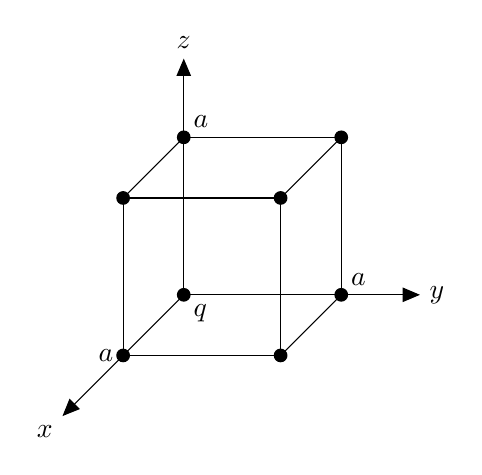
\begin{tikzpicture}[>=triangle 45]
        \draw[->] (0,0,0) -- (3,0,0) node[right] {$y$};
        \draw[->] (0,0,0) -- (0,3,0) node[above] {$z$};
        \draw[->] (0,0,0) -- (0,0,4) node[below left] {$x$};
        \draw[-]  (0,2,0) -- (2,2,0) {};
        \draw[-]  (0,2,0) -- (0,2,2) {};
        \draw[-]  (2,0,0) -- (2,2,0) {};
        \draw[-]  (2,0,0) -- (2,0,2) {};
        \draw[-]  (0,0,2) -- (0,2,2) {};
        \draw[-]  (0,0,2) -- (2,0,2) {};
        \draw[-]  (2,2,0) -- (2,2,2) {};
        \draw[-]  (2,0,2) -- (2,2,2) {};
        \draw[-]  (0,2,2) -- (2,2,2) {};
        \filldraw[black] (0,0,0) circle (0.8mm);
        \filldraw[black] (0,2,0) circle (0.8mm);
        \filldraw[black] (0,0,2) circle (0.8mm);
        \filldraw[black] (2,0,0) circle (0.8mm);
        \filldraw[black] (2,2,2) circle (0.8mm);
        \filldraw[black] (0,2,2) circle (0.8mm);
        \filldraw[black] (2,0,2) circle (0.8mm);
        \filldraw[black] (2,2,0) circle (0.8mm);
        \node at (0,2,0) [above right] {$a$};
        \node at (0,0,2) [left] {$a$};
        \node at (2,0,0) [above right] {$a$};
        \node at (0,0,0) [below right] {$q$};
    \end{tikzpicture}}
    \caption{Wangsness 2-3}
    \label{fig:EMAG_1_Wangsness_2_3}
  \end{subfigure}
  \begin{subfigure}[b]{0.49\textwidth}
    \centering
    \resizebox{\textwidth}{!}{
    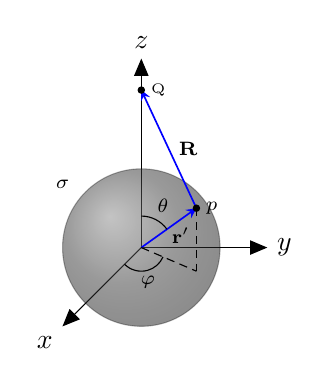
\begin{tikzpicture}[>=triangle 45]
        \draw[->] (0,0,0) -- (1.6,0,0) node[right] {$y$};
        \draw[->] (0,0,0) -- (0,2.4,0) node[above] {$z$};
        \draw[->] (0,0,0) -- (0,0,2.6) node[below left] {$x$};
        \filldraw[ball color=gray!90!white,opacity=0.3] (0,0,0) circle (1);
        \coordinate (z) at (0,1,0) {};
        \coordinate (x) at (0,0,1) {};
        \coordinate (o) at (0,0,0) {};
        \coordinate (p) at (0.7,0.5,0) {};
        \coordinate (p1) at (0.7,-0.3,0) {};
        \coordinate (Q) at (0,2,0) {};
        \node at (Q) [right] {\tiny{Q}};
        \node at (p) [right] {\scriptsize{$p$}};
        \node at (-1,0.8,0) {\scriptsize{$\sigma$}};
        \node at (0.5,0.15,0) {\scriptsize{$\mathbf{r}'$}};
        \draw[->,>=stealth,draw=blue,semithick] (o) -- (p);
        \draw[-,densely dashed,draw=black] (o) -- (p1);
        \draw[-,densely dashed,draw=black] (p) -- (p1);
        \draw[->,>=stealth,draw=blue,semithick] (p) -- node[right] {\scriptsize{$\mathbf{R}$}}(Q);
        \filldraw[black] (Q) circle (0.4mm);
        \filldraw[black] (p) circle (0.4mm);
        \pic[draw=black, -, "\scriptsize{$\theta$}", angle eccentricity=1.5,angle radius = 0.4cm] {angle = p--o--z};
        \pic[draw=black, -, "\scriptsize{$\varphi$}", angle eccentricity=1.5,angle radius = 0.3cm] {angle = x--o--p1};
    \end{tikzpicture}}
    \caption{Drawing for Wangsness 2-8}
    \label{fig:EMAG_1_wangsness_2_8}
  \end{subfigure}
\end{figure}
\begin{problem}[Wangsness 2-8]
    Consider the sphere in Fig.~\subref{fig:EMAG_1_wangsness_2_8} or radius $a$ with a constant surface change density $\sigma$. What is the total charge $Q'$ on the sphere? Find the force produced by this charge distribution on a point $q$ on the $z$ axis for both $z>a$ and $z<a$.
\end{problem}
\begin{proof}[Solution]
We have that:
\begin{equation*}
    Q' = \iint_{S} \sigma da = \sigma \iint_{S}da = \sigma 4\pi a^{2}
\end{equation*}
The relative position vector $\mathbf{R}$ of the point $Q$ with respect to a point $\mathbf{r}'$ on the sphere is $z\hat{\mathbf{z}} - a\hat{\mathbf{r}}'$. So we have:
\begin{equation*}
    \mathbf{F}_q = \frac{q}{4\pi \epsilon_0} \iint_{S} \frac{\sigma da'\mathbf{R}}{R^3}=\frac{q\sigma}{4\pi \epsilon_0} \int_{0}^{2\pi} \int_{0}^{\pi} \frac{(z\hat{\mathbf{z}}-a\hat{\mathbf{r}}')a^2\sin(\theta')d\theta ' d\varphi '}{\big(z^2+a^2-2az\cos(\theta')\big)^{3/2}}    
\end{equation*}
Writing $\hat{\mathbf{r}}' = \sin(\theta')\cos(\varphi')\hat{\mathbf{x}} + \sin(\theta')\sin(\varphi')\hat{\mathbf{y}}+\cos(\theta')\hat{\mathbf{z}}$ leads us to conclude the $x$ and $y$ component vanish as $\int_{0}^{2\pi} \cos(\varphi')d\varphi' = \int_{0}^{2\pi}\sin(\varphi')d\varphi' = 0$. Thus, we have: 
\begin{equation*}
    \mathbf{F}_q = \frac{q\sigma\hat{\mathbf{z}}}{4\pi \epsilon_{0}}\int_{0}^{2\pi}\int_{0}^{\pi}\frac{\big(z-a\cos(\theta)\big)a^{2}\sin(\theta')}{\big(z^{2}+a^{2}-2az\cos(\theta')\big)^{3/2}}d\theta' d\varphi'
\end{equation*}
Let $u = cos(\theta')$. Then $du = -\sin(\theta')d\theta'$. We obtain:
\begin{align*}
    \mathbf{F}_{q} &= a^{2}\frac{q\sigma \hat{\mathbf{z}}}{2\epsilon_{0}}\int_{-1}^{1}\frac{u}{\big(z^{2}+a^{2}-2azu\big)^{3/2}}du\\
    &= a^{2}\frac{q\sigma \hat{\mathbf{z}}}{2\epsilon_{0}}\int_{-1}^{1}\frac{\partial}{\partial z} \bigg(\frac{1}{\sqrt{a^{2}+z^{2}-2azu}}\bigg)du\\
    &= a^{2}\frac{q\sigma \hat{\mathbf{z}}}{2\epsilon_{0}}\frac{\partial}{\partial z} \int_{-1}^{1}\frac{1}{\sqrt{a^{2}+z^{2}-2azu}}du\\
    &= a^{2}\frac{q\sigma \hat{\mathbf{z}}}{2\epsilon_{0}}\frac{\partial}{\partial z} \bigg[\frac{1}{za}\sqrt{a^{2}+z^{2}-2azu}\bigg]_{-1}^{1}\\
    &= a^{2}\frac{q\sigma \hat{\mathbf{z}}}{2\epsilon_{0}} \frac{\partial}{\partial z}\bigg(\frac{|z-a|-|z+a|}{az}\bigg)
\end{align*}
Now, if $z>a$, then $|z-a|-|z+a| = (z-a)-(z+a) = -2a$, and thus:
\begin{equation*}
    \mathbf{F}_{q} = a^{2}\frac{q\sigma}{\epsilon_{0}z^{2}}\hat{\mathbf{z}} = \frac{qQ}{4\pi \epsilon_{0}z^{2}} \tag{$z>a$}
\end{equation*}
If $z<a$, then $|z-a|-|z+a| = 2z$, and thus:
\begin{equation*}
    \mathbf{F} = \mathbf{0} \tag{$z<a$}
\end{equation*}
\end{proof}
\begin{problem}[Wangsness 2-7]
Given a line change of length $L$ with constant charge density lying along the positive $z$ axis with its ends located at $z_{0}$ and $z_{0}+L$, find the total force exerted on this by a uniform spherical charge distribution with center at the origin and radius $a<z_{0}$.
\end{problem}
\begin{proof}[Solution]
If the charge is distributed over a length $L$ along the $z$-axis with charge per unit length $\lambda$, the force over the length $L$ is given by:
\begin{equation*}
    \mathbf{F}_{Lz} = \frac{\rho a^3}{3\epsilon_0}\hat{\mathbf{z}} \int_{z_0}^{z_0+L} \frac{\lambda dz}{z^2} = \frac{\rho \lambda a^3}{3\epsilon_0}\bigg(\frac{L}{z_0(z_0+L)}\bigg) \hat{\mathbf{z}}
\end{equation*}
\end{proof}
\begin{problem}[Wangsness 3-9]
Given two infinite plane sheets with equal and opposite constant surface charge densities $\sigma$ that are parallel and a distance $\pm a$ to the $xy$ plane, find $\mathbb{E}$ everywhere.
\end{problem}
\begin{proof}[Solution]
For an infinite sheet
\begin{equation*}
    \mathbf{E} = \frac{\sigma}{2\epsilon_0}    
\end{equation*}
Using the principle of superposition, we get:
\begin{equation*}
    \mathbf{E} = \begin{cases} 0, & |z|>a \\ -\frac{\sigma}{\epsilon_0}\hat{\mathbf{z}},& |z|\leq a\end{cases}
\end{equation*}
\end{proof}
\subsubsection{Wangsness 3-10}
$\hat{\mathbf{E}} = \frac{\lambda}{4\pi\epsilon_0} \int \frac{dl \hat{\mathbf{r}}}{R^2} = \frac{\lambda}{4\pi \epsilon_0} \int \frac{ad\phi' \hat{\mathbf{r}}}{a^2+z^2}$. And $\hat{\mathbf{r}} = \frac{\mathbf{R}}{R} = \frac{-\rho' \hat{\boldsymbol{\uprho}}+z\hat{\mathbf{z}}}{\sqrt{a^2+z^2}} = \frac{-a\cos(\phi')\hat{\mathbf{x}}-a\sin(\phi')\hat{\mathbf{y}}+z\hat{\mathbf{z}}}{\sqrt{a^2+z^2}}$. So, we thus obtain the following: \\ $\mathbf{E} = \frac{\lambda}{4\pi \epsilon_0} \int_{-\alpha}^{\alpha} \frac{-a\cos(\phi')\hat{\mathbf{x}}-a\sin(\phi')\hat{\mathbf{y}}+z\hat{\mathbf{z}}}{\sqrt{a^2+z^2}}ad\phi' = \frac{\lambda a\big[ -a\sin(\alpha)\hat{\mathbf{x}}+z\alpha \hat{\mathbf{z}}\big]}{2\pi \epsilon_0 (a^2+z^2)^{3/2}}$. If $\alpha = \pi$, we get $\mathbf{E} = \frac{\lambda a z}{2\epsilon_0 (a^2+z^2)^{3/2}}\hat{\mathbf{z}}$
\subsection{Homework V}
\subsubsection{Wangsness 4-3}
For $\rho<\rho_0$, choose a Gaussian cylinder concentric with the line. We have that $\oiint \mathbf{E}\cdot \mathbf{da} = \frac{Q_{in}}{\epsilon_0}$ from Gauss' Law, and from symmetry we have $\oiint \mathbf{E}\cdot \mathbf{da} = E(2\pi \rho \ell)$. So, $\mathbf{E} = \frac{\lambda}{2\pi \epsilon_0 \rho}\hat{\boldsymbol{\uprho}}$.
\begin{figure}[htbp]
\begin{center}
\includegraphics[scale=0.5]{4-3.png}
\end{center}
\caption{Drawing for 4-3}
\end{figure}
For $\rho>\rho_0$, choose a similar Gaussian cylinder. We get $\oiint \mathbf{E}\cdot \mathbf{da} = \frac{Q_{in}}{\epsilon_0}$, and thus $\mathbf{E} = \frac{\lambda \ell + \sigma 2\pi \rho_0 \ell}{2\pi \epsilon_0 \rho \ell}\hat{\boldsymbol{\uprho}} = \frac{\lambda+2\pi \rho_0 \sigma}{2\pi \epsilon_0 \rho}\hat{\boldsymbol{\uprho}}$. To make $\hat{\mathbf{E}} = \mathbf{0}$ for $\rho>\rho_0$, we need $\sim = \frac{-\lambda}{2\pi \rho_0}$. Thus, it is possible for such a scenario to occur.
\subsubsection{Wangsness 4-5}
For $r>a$, $\oiint \mathbf{E}\cdot \mathbf{da} = \frac{Q_{in}}{\epsilon_0} \Rightarrow E(4\pi r^2) = \iiint A r'^{1/2}r'^2 \sin(\theta ')dr'd\theta'd\phi' = 4\pi \frac{2}{7}\frac{a^{7/2}}{\epsilon_0}A$. Thus, from symmetry, $\mathbf{E} = \frac{2A a^{7/2}}{7 \epsilon_0 r^2}\hat{\mathbf{r}}$, where $r>a$. For $r<a$. $E(4\pi r^2) = 4\pi A \frac{2}{7}r^{7/2}$, and thus $\mathbf{E} = \frac{2Ar^{3/2}}{7\epsilon_0}\hat{\mathbf{r}}$. 
\begin{figure}
  \begin{subfigure}[b]{0.49\textwidth}
     \centering
    \includegraphics[width=\textwidth]{4-5-1.png}
  \end{subfigure}
  \begin{subfigure}[b]{0.49\textwidth}
    \centering
    \includegraphics[width=\textwidth]{4-5-2.png}
  \end{subfigure}
  \caption{Drawings for Wangsness 4-5}
\end{figure}
\subsubsection{Wangsness 4-6}
For $r<a$, $\oiint\mathbf{E} \cdot \mathbf{da} = 0$, and from symmetry we conclude $\mathbf{E} = \mathbf{0}$. For $a\leq r \leq b$, $\oiint \mathbf{E}\cdot \mathbf{da} = \frac{Q_{in}}{\epsilon_0} = \frac{\rho_c(\frac{4}{3}\pi)(r^3-a^3)}{\epsilon_0}$, where $\rho_c$ is the charge density and is equal to $\frac{Q}{\frac{4}{3}\pi(b^3-a^3)}$, and thus $\mathbf{E} = \frac{Q}{4\pi \epsilon_0 r^2}\bigg(\frac{r^3-a^3}{b^3-a^3}\bigg)\hat{\mathbf{r}}$. For $r\geq b$, this is similar to the uniform sphere problem. Indeed, $\oiint \mathbf{E}\cdot \mathbf{da} = \frac{Q_{in}}{\epsilon_0} = \frac{Q}{4\pi \epsilon_0 r^2}$.
\subsubsection{Wangsness 4-7}
Choose as a Gaussian surface a cylinder of length $L$ and radius $\rho$ that is concentric with the infinite cylinder. For $\rho<a$, $\oiint \mathbf{E}\cdot \mathbf{da} = \frac{Q_{in}}{\epsilon_0}$. Now $\oiint \mathbf{E} \cdot \mathbf{da} = \iint_{Right\ Side} \mathbf{E}\cdot \mathbf{da} + \iint_{Left\ Side}\mathbf{E}\cdot \mathbf{da} + \iint_{Cylinder} \mathbf{E}\cdot \mathbf{da}$. From symmetry, we have that $\mathbf{E}$ and $\mathbf{da}$ are orthogonal along the left and right faces of the cylinder, leaving only the cylindrical body left to integrate over. We get $E(2\pi \rho L) = \frac{\rho_c \pi \rho^2 L}{\epsilon_0}$, where $\rho_c$ is the charge density. Combining this together, we obtain $\mathbf{E} = \frac{\rho_c \rho}{2\epsilon_0} \hat{\boldsymbol{\uprho}}$. For $\rho>a$, $\mathbf{E} = \frac{\rho_{c} a^2}{2\epsilon_0 \rho}\hat{\boldsymbol{\uprho}}$. We see that the electric field goes like $\frac{1}{\rho}$, which is consistent with the result obtained from $4-11$.
\subsubsection{Wangsness 4-11}
$\mathbf{E} = E_0 \big(\frac{\rho}{a}\big)^3 \hat{\boldsymbol{\uprho}}$ for $0 < \rho < a$, and $\mathbf{E} = 0$ otherwise. Thus, $\nabla \cdot \mathbf{E} = \frac{1}{\rho} \frac{\partial}{\partial \rho}\big(\rho E_{\rho}\big) + \frac{1}{\rho} \frac{\partial E_{\phi}}{\partial \phi} + \frac{\partial E_z}{\partial z}$ = $\frac{4E_0 \rho^2}{a^3}$. From Gauss' Law, $\nabla \cdot \mathbf{E} = \frac{\rho_c}{\epsilon_0}$. Thus, $\rho_c = \epsilon_0 \nabla \cdot \mathbf{E} = \frac{4\epsilon_0 E_0 \rho^2}{a^3}$ for $\rho<a$. For $\rho>a$, $\nabla \cdot \mathbf{E} = \nabla \cdot \mathbf{0} = 0$, and thus $\rho_c = 0$.
\subsubsection{Wangsness 4-12}
$\mathbf{E} = E_r \hat{\mathbf{r}}+E_{\theta} \hat{\boldsymbol{\uptheta}}$, where $E_r = \frac{2A\cos(\theta)}{r^3}$ and $E_{\theta} = \frac{A\sin(\theta)}{r^3}$. From Gauss' Law, $\nabla \cdot \mathbf{E} = \frac{\rho_c}{\epsilon_0}$, and thus $\rho_c = \epsilon_0 \nabla \cdot \mathbf{E}$. But $\nabla \cdot \mathbf{E} = 0$, and thus $\rho_c = 0$.
\subsection{Homework VI}
\subsubsection{Wangsness 5-1}
$\mathbf{E} = (yz-2x)\hat{\mathbf{x}}+xz\hat{\mathbf{y}}+xy\hat{\mathbf{z}}$. So, $\nabla \times \mathbf{E} = (x-x)\hat{\mathbf{x}}-(y-y)\hat{\mathbf{y}}+(z-z)\hat{\mathbf{z}} = \mathbf{0}$. Therefore $\mathbf{E}$ is a possible electrostatic field. Indeed, writen $\mathbf{E} = \nabla(\phi)$, we get $-\frac{\partial \phi}{\partial x} = yz-2x$, so $-\phi = xyz - x^2 + g(y,z)$, where $g$ is a function of $y$ and $z$ (Note: $\frac{\partial g}{\partial x} = 0$ as $g$ is not a function of $x$). Now $-\frac{\partial \phi}{\partial y} = xz$ and $-\frac{\partial \phi}{\partial z} = xy$, and thus $g(y,z) = constant$. So, $\phi(x,y,z) = -xyz+x^2 + C$, where $C$ is some constant. We may choose $C$ is we desire, so let $C=0$ to make things easy. The integral $\int \mathbf{E}\cdot \mathbf{d\ell}$ from the origin $(0,0,0)$ to a point $(x,y,z)$ is thus independent of path and may be computed by using the fundamental theorem of gradients. That is, $\int \mathbf{E}\cdot \mathbf{d\ell} = -\int _{(0,0,0)}^{(x,y,z)} \nabla(\phi)\cdot \mathbf{d\ell} = -\big(\phi(x,y,z) -\phi(0,0,0)\big) = \phi(0,0,0)-\phi(x,y,z)$. Now, $\phi(0,0,0)= 0$, and thus $\int_{(0,0,0)}^{(x,y,z)}\mathbf{E}\cdot \mathbf{d\ell} = -\phi(x,y,z) = xyz-x^2$.
\subsubsection{Wangsness 5-3}
$\phi = \frac{1}{4\pi \epsilon_0}\big[ \frac{q}{R_{+}} - \frac{q}{R_{-}}\big] = \frac{q}{4\pi \epsilon_0}\big[\frac{1}{\sqrt{x^2+y^2+(z-a)^2}}-\frac{1}{\sqrt{x^2+y^2+(z+a)^2}}\big]$. At $z=0$, we get $\phi = \frac{q}{4\pi \epsilon_0}\big[ \frac{1}{\sqrt{x^2+y^2+a^2}}-\frac{1}{\sqrt{x^2+y^2+a^2}}\big] = 0$. Thus, the entire $xy-$plane is an equipotential surface with $\phi = 0$.
\begin{figure}[htbp]
  \centering
    {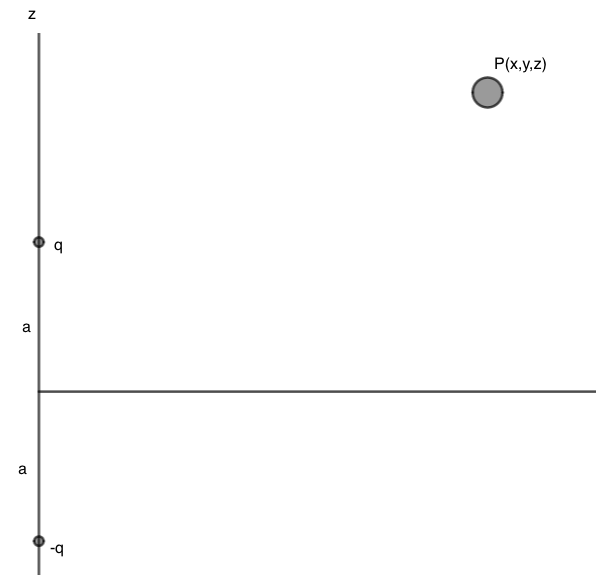
\includegraphics[scale=0.4]{5-3.png}}
    \caption{Drawing for Wangsness 5-3}
\end{figure}
\subsubsection{Wangsness 5-4}
$\phi = \frac{1}{4\pi \epsilon_0} \sum \frac{q_i}{R_i} = \frac{1}{4\pi \epsilon_0}\bigg[ \frac{q}{\sqrt{a^2/4}}+\frac{2q}{\sqrt{a^2/2}}-\frac{4q}{\sqrt{a^2/2}}+\frac{3q}{\sqrt{a^2/2}}\bigg] = \frac{q}{\sqrt{2}\pi \epsilon_0 a}$. To know $\mathbf{E}$ from $\phi$, $\phi$ must be known in some region about the point, not just at the point. To be precise in mathematical terms, we must know $\phi$ in some open set about the point in order to compute $\nabla(\phi)$. This is analogous to functions in calculus. Suppose $f$ is a function and $a$ is a real number, and suppose we know the value of $f(a)$. Can we determine what $f'(a)$ is? The answer is no, there is not enough information. If we know what $f(x)$ is in some interval $(a-\epsilon,a+\epsilon)$, then we can compute $f'(a)$.
\begin{figure}[htbp]
    \centering
    {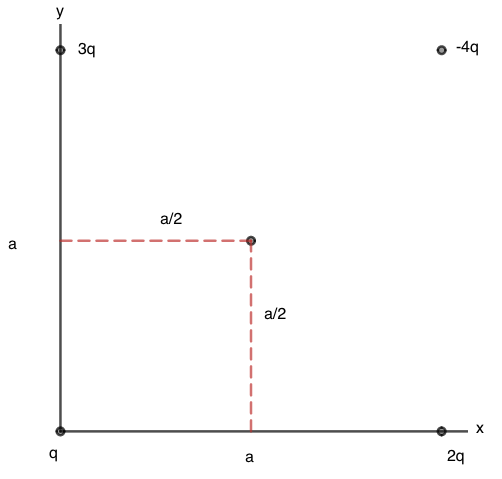
\includegraphics[scale=0.4]{5-4.png}}
    \caption{Drawing for Wangsness 5-4}
\end{figure}
\subsubsection{Wangsness 5-10}
We know that $\mathbf{E} = \begin{cases} \frac{2A a^{7/2}}{7\epsilon_0 r^2}\hat{\mathbf{r}}, & r>a \\ \frac{2A r^{3/2}}{7\epsilon_0}, & r<a\end{cases}$. So, $\Delta \phi = \int \mathbf{E} \cdot \mathbf{d\ell}$. Now, $\mathbf{d\ell} = -dr(-\hat{\mathbf{r}}) = \mathbf{dr}$. We split the integral into two parts and compute: $\int \mathbf{E}\cdot \mathbf{d\ell} = \int_{0}^{a} \mathbf{E}\cdot \mathbf{dr} + \int_{a}^{\infty} \mathbf{E}\cdot \mathbf{dr} = \frac{4A a^{5/4}}{35 \epsilon_0}\bigg[ \frac{7}{2}-\big(\frac{r}{a}\big)^{7/2}\bigg]$.
\subsubsection{Wangsness 5-11}
We have that $\mathbf{E} = \begin{cases} \mathbf{0}, & r<a\\ \frac{Q}{4\pi \epsilon_0}\bigg(\frac{r^3-a^3}{b^3-a^3}\bigg)\hat{\mathbf{r}}, & a\leq r \leq b\\ \frac{Q}{4\pi \epsilon_0 r^2}\hat{\mathbf{r}}, & r>b\end{cases}$ We thus split the integral into three regions and compute: $\Delta\phi=\int \mathbf{E}\cdot \mathbf{d\ell} = \int_{0}^{a} \mathbf{E}\cdot \mathbf{dr}+\int_{a}^{b} \mathbf{E}\cdot \mathbf{dr}+\int_{b}^{\infty} \mathbf{E}\cdot \mathbf{dr}$. We then obtain $\phi(\mathbf{r}) = \begin{cases} \frac{\rho_c(b^3-a^3)}{3\epsilon_0 r}, & r>b \\ \frac{\rho}{3\epsilon_0}\bigg[ \frac{3}{2}b^2-\frac{r^2}{2}-\frac{a^3}{r}\bigg], & a\leq r \leq b\\ \frac{\rho_c}{2\epsilon_0}(b^2-a^2), & r<a\end{cases}$
\subsubsection{Wangsness 5-14}
$\phi = \frac{1}{4\pi \epsilon_0}\iint \frac{\sigma_c da'}{R}$. Here, $R = |\mathbf{r}-\mathbf{r}'| = \sqrt{a^2+r^2-2ar\cos(\theta')}$, and $da' = a^2\sin(\theta')d\theta'd\phi'$. So, we have $\phi = \frac{\sigma_c}{4\pi \epsilon_0}\int_{0}^{2\pi}\int_{0}^{\pi} \frac{a^2\sin(\theta')d\theta' d\phi'}{\sqrt{a^2+r^2-2ar\cos(\theta')}} = \frac{\sigma_c a^2}{2\epsilon_0}\int_{0}^{\pi} \frac{\sin(\theta')d\theta'}{\sqrt{a^2-r^2-2ar\cos(\theta')}}$. Let $u = \cos(\theta')$. Then $du = -\sin(\theta')d\theta'$, and we have $-\int\frac{du}{\sqrt{a^2+r^2-2aru}}$. Note that $r$ and $a$ are constants in the integral, and thus this can be computed by trigonometric substitution (Or wolframalpha/integral tables if you're lazy). We thus have $\phi(\mathbf{r}) = \begin{cases}\frac{a^2\sigma}{\epsilon_0 r}, & r>a \\ \frac{a\sigma}{\epsilon_0}, & r<a\end{cases}$.
\subsection{Homework VII}
\subsubsection{Wangsness 6-6}
Before the connection, $Q=C_1 \Delta \phi$. After the connection, $Q_1 = C_1 \Delta\phi'$, $Q_2 = C_2 \Delta \phi'$, $Q_1+Q_2=Q$, and $Q_1+Q_2=(C_1+C_2)\Delta \phi' = Q = C_1\Delta \phi$. Thus, $\Delta \phi' = \frac{C_1}{C_1+C_2}\Delta \phi$, $Q_1 = \frac{C_1^2}{C_1+C_2}\Delta \phi$, and $Q_2 = \frac{C_1 C_2}{C_1+C_2}\Delta \phi$.
\subsubsection{Wangsness 6-7}
For Parallel:\\
$Q_1 = C_1\Delta \phi$, $Q_2 = C_2\Delta \phi$, where $Q_1$ and $Q_2$ are the charges on the plates $C_1$ and $C_2$, respectively. The total charge is $Q_1+Q_2$. Thus, $Q=Q_1+Q_2 = C_1\Delta\phi + C_2 \Delta \phi =(C_1+C_2)\Delta\phi = C_p \Delta \phi$, where $C_p$ is $C_1+C_2$. \\
For Series:\\
$\Delta \phi = \Delta\phi_1 + \Delta \phi_2$, where $\Delta\phi_1$ and $\Delta \phi_2$ are the potential differences across $C_1$ and $C_2$, respectively. If a charge $Q$ is on the left plate of $C_1$, then there is a charge $-Q$ on the right plate, and therefore there is a charge $Q$ on the left plate of $C_2$ as well. Thus, $Q=Q_1=Q_2$. So, $\Delta \phi = \frac{Q_1}{C_1} + \frac{Q_2}{C_2} = \frac{Q}{C_1}+\frac{Q}{C_2} = Q\big(\frac{1}{C_1}+\frac{1}{C_2}\big) = \frac{Q}{C_s}$, where $\frac{1}{C_s} = \frac{1}{C_1}+\frac{1}{C_2}$.
\subsubsection{Wangsness 6-9}
At $r=a$, $E=\frac{Q}{4\pi \epsilon_0 a^2}$, $Q=C\Delta \phi$, and $C=\frac{4\pi \epsilon_0 ab}{b-a}$. Thus, we may write $E$ as $E=\frac{b\Delta \phi}{a(b-a)}$. To minimize this, we solve $\frac{\partial E}{\partial a} = 0$. This gives us $a=\frac{b}{2}$. To check that is is a minimum, we check $\frac{\partial^2 E}{\partial a^2}\bigg|_{a=\frac{b}{2}}$. This gives us $\frac{32\Delta \phi}{b}$, which is positive. Therefore $a=\frac{b}{2}$ is a minimum.
\subsubsection{Wangsness 6-10}
$E=\frac{\lambda}{2\pi \epsilon_0 \rho}$, where $\lambda$ is the linear charge density, $\lambda = \frac{Q}{L}$. Thus, $\Delta\phi = - \int_{b}^{a} \frac{\lambda}{2\pi \epsilon_0\rho}d\rho = \frac{\lambda}{2\pi \epsilon_0}\ln\big(\frac{b}{a}\big)$. We have that $C=\frac{Q}{\Delta\phi}$, and thus $C = \frac{2\pi \epsilon_0 L}{\ln\big(\frac{b}{a}\big)}$
\subsection{Homework VIII}
\subsubsection{Wangsness 7-2}
$U_e = \underset{All\ Pairs}\sum\frac{q_i q_j}{r\pi \epsilon_0 R_{ij}}$, where $R_{ij} = |\mathbf{r}_i-\mathbf{r}_j| = \sqrt{r_i^2+r_j^2 -2\mathbf{r}_i\cdot \mathbf{r}_j}$. Computing the sum, we get $U_e = \frac{q^2}{4\pi \epsilon_0 a}\big(12 + \frac{12}{\sqrt{2}}+\frac{4}{\sqrt{3}}\big)$.
\begin{figure}[htbp]
    \centering
    {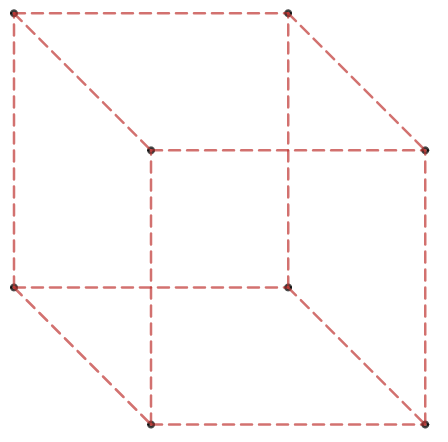
\includegraphics[scale=0.4]{7-2.png}}
    \caption{Drawing for Wangsness 7-2}
\end{figure}
\subsubsection{Wangsness 7-4}
$\rho_c = Ar^n$, where $A$ is a constant and $n\geq 0$. Thus, $U_e = \frac{1}{2} \int \rho_c(\mathbf{r})\phi(\mathbf{r})d\tau$. We have that $E = \frac{Aa^{n+3}}{\epsilon_0 (n+3)r^2}$ for $r\geq a$, and $E=\frac{Ar^{n+1}}{\epsilon_0(n+3)}$ for $r\leq a$ from Gauss' Law. Now, all of the charges are located within $r\leq a$, and so we must compute $\phi$ in this region. Letting $\phi(r)\rightarrow 0$ as $r\rightarrow \infty$, we may compute $\phi$ as $\phi(r) = -\int_{\infty}^{r}\mathbf{E}\cdot \mathbf{d\ell} = -\int_{\infty}^{a} \mathbf{E}\cdot \mathbf{d\ell} - \int_{a}^{r}\mathbf{E}\cdot \mathbf{d\ell} = \frac{Aa^{n+3}}{\epsilon_0(n+3)a}+\frac{Aa^{n+2}}{\epsilon_0(n+2(n+3)}-\frac{Ar^{n+2}}{\epsilon_0(n+3)(n+2)}$. We can now compute  the potential energy. $U_e =\frac{1}{2}\int \rho_c(\mathbf{r})\phi(\mathbf{r})d\tau = \int_{0}^{2\pi} \int_{0}^{\pi}\int_{0}^{a} A r^n \bigg(\frac{Aa^{n+3}}{\epsilon_0(n+3)a}+\frac{Aa^{n+2}}{\epsilon_0(n+2)(n+3)}-\frac{Ar^{n+2}}{\epsilon_0(n+3)(n+2)}\bigg)r^2 \sin(\theta)dr d\theta d\phi = \frac{2\pi A^2}{\epsilon_0 (n+3)}\bigg[\frac{a^{2n+5}}{n+3}+\frac{a^{2n+5}}{(n+2)(n+3)}-\frac{a^{2n+5}}{(n+2)(2n+5)}\bigg]$. Taking the limit as $n\rightarrow 0$, we get $\frac{3}{5}\bigg[\frac{Q^2}{4\pi \epsilon_0 a}\bigg]$, as expected for a constant spherical charge density.
\subsubsection{Wangsness 7-6}
\begin{figure}[htbp]
    \centering
    {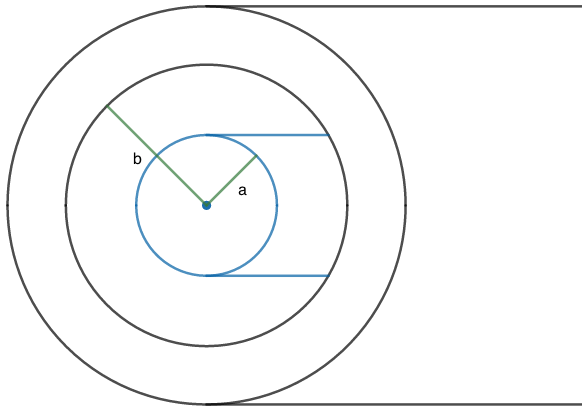
\includegraphics[scale=0.4]{7-6.png}}
    \caption{Drawing for Wangsness 7-6}
\end{figure}
$U_e = \frac{1}{2}\int_{S}\sigma_c(\mathbf{r})\phi(\mathbf{r})da$. In the region between the cylinders we have that $E = \frac{\lambda}{2\pi \epsilon_0 \rho}$, and thus $\phi= \frac{\lambda 2\pi \epsilon_0}\ln\big(\frac{\rho_0}{\rho}\big)$, where $\rho_0$ is the zero of $\phi$. We can now compute $U_e$ and we get $U_e = \frac{\lambda L}{4\pi \epsilon_0}\ln\big(\frac{b}{a}\big)$. As $U_e = \frac{1}{2}\frac{Q^2}{C}$, we get $C= \frac{2\pi \epsilon_0 L}{\ln\big(\frac{b}{a}\big)}$
\subsubsection{Wangsness 7-9}
The electric field is $\mathbf{E}_i = \frac{Qr}{4\pi \epsilon_0 a^3}\hat{\mathbf{r}}$ inside the distribution, and $\mathbf{E}_o = \frac{Q}{4\pi\epsilon_0r^2}\hat{\mathbf{r}}$. The energy density inside is thus $\mu_{e_i} = \frac{1}{2}\epsilon_0 E_i^2=\frac{Q^2r^2}{32\pi^2 \epsilon_0 a^6}$ and outside is $\mu_{e_o} = \frac{1}{2}\epsilon_0 E_0^2 = \frac{Q^2}{32\pi^2 \epsilon_0 r^4}$. The total energy is $\int_{Inside} \mu_{e_i}d\tau + \int_{Outside} \mu_{e_o}d\tau$. Computing this integral, we get $U_e = \frac{3}{5}\bigg( \frac{Q^2}{4\pi \epsilon_0}\bigg)$, in agreement with before.
\subsubsection{Wangsness 7-10}
$U_e = \frac{\epsilon_0}{2} \underset{All\ Space}\int E^2 d\tau$. The $\mathbf{E}-$Field in between the spheres is $\frac{Q}{4\pi \epsilon_0 r^2}\hat{\mathbf{r}}$. The energy associated to this region is thus $\int_{0}^{2\pi}\int_{0}^{\pi}\int_{a}^{b} \frac{\epsilon}{2} \frac{Q^2}{16\pi^2 \epsilon_0^2 r^4}r^2\sin(\theta) dr d\theta d\phi = \frac{Q^2}{8\pi \epsilon_0}\bigg(\frac{b-a}{ab}\bigg)$. We have that $C = \frac{1}{2} \frac{Q^2}{U_e}$, and thus $C = \frac{4\pi \epsilon_0 ab}{b-a}$.
\subsubsection{Wangsness 7-17}
$\mathbf{E} = \frac{\lambda}{2\pi \epsilon_0 \rho}\hat{\boldsymbol{\uprho}}$, $\Delta\phi = \frac{\lambda}{2\pi \epsilon_0 \ln\big(\frac{b}{a}\big)}$, and therefore $\lambda = \frac{2\pi \epsilon_0 \Delta\phi}{\ln\big(\frac{b}{a}\big)}$ and $E = \frac{\Delta \phi}{\rho \ln\big(\frac{b}{a}\big)}$. So, $f_e = \mu_e = \frac{1}{2} \epsilon_0 E^2\bigg|_{\rho = a} = \frac{1}{2} \epsilon_0 \bigg[ \frac{\Delta\phi}{a \ln\big(\frac{b}{a}\big)}$. Thus, $\mathbf{F}_{Tot} = \int f_e \mathbf{da} = f_e \int \mathbf{da} = 0$.
\subsection{Homework IX}
\subsubsection{Wangsness 8-5}
The monopole moment is $Q = \sum q_i = -3q-2q-q+q+2q+3q+4q+5q=9q$.
The dipole moment is $\mathbf{p} = \sum q_i \hat{\mathbf{r}}_i = (-3q)\mathbf{0} + (-2q)a\hat{\mathbf{x}} + (-q)(a\hat{\mathbf{x}}+a\hat{\mathbf{y}})+qa\hat{\mathbf{y}} + 2q(a\hat{\mathbf{y}}+a\hat{\mathbf{z}})+3q(a\hat{\mathbf{x}}+a\hat{\mathbf{y}}+a\hat{\mathbf{z}})+4q(a\hat{\mathbf{x}}+a\hat{\mathbf{z}})+5qa\hat{\mathbf{z}}=4qa\hat{\mathbf{x}}+5qa\hat{\mathbf{y}}+14aq\hat{\mathbf{z}}$
\begin{figure}[htbp]
    \centering
    {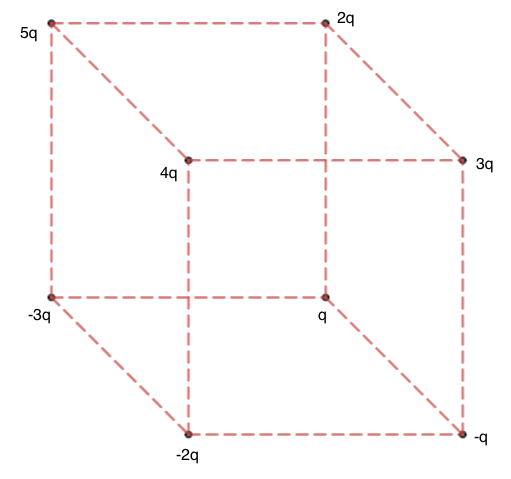
\includegraphics[scale=0.4]{8-5.png}}
    \caption{Drawing for Wangsness 8-5}
\end{figure}
It is possible to find an origin about which the dipole moment will vanish. Consider an arbitrary charge distribution with the center of charge designated as c.c. The position vector of this is $\mathbf{r}_{c.c.} = \frac{\int \mathbf{r}' \rho d\tau '}{\int \rho d\tau '} = \frac{\sum \mathbf{r}_i q_i}{\sum q_i}$. Shifting the origin by $\mathbf{r}_{c.c.}$ the dipole moment becomes zero. The original dipole moment is $\mathbf{p}_{o} = \int \mathbf{r}' d\tau ' = \sum \mathbf{r}_i q_i$. The new dipole moment will be $\mathbf{p}_N = \int (\mathbf{r}' - \mathbf{r}_{c.c.})d\tau' = \int \mathbf{r}' d\tau' - \mathbf{r}_{c.c.} \int \rho d\tau' = \sum \mathbf{r}_i q_i - \mathbf{r}_{c.c} \sum q_i = \sum \mathbf{r}_i q_i - \frac{\sum \mathbf{r}_i q_i }{\sum q_i}\sum q_i = \mathbf{0}$. For the problem at hand, this equates to $\mathbf{r}_{c.c} = \langle \frac{4}{9}a, \frac{5}{9}a, \frac{14}{9}a\rangle$ (In Cartesian Coordinates).
\begin{problem}[Wangsness 8-8]
\end{problem}
\begin{proof}[Solution]
\begin{equation*}
    Q = \int_{S'} \sigma da'= \int_{0}^{2\pi} \sin(\theta)\cos(\theta)d\theta = \int_{0}^{2\pi} \int_{0}^{\pi} \sigma_{0} \cos(\theta) a^2 \sin(\theta) d\theta d\phi = 2\pi \sigma_{0} = 0
\end{equation*}
\begin{align*}
    \mathbf{p} &= \int_{S'}\sigma \mathbf{r}' da'\\
    &= \sigma a^{3}\int_{0}^{2\pi} \int_{0}^{\pi} \cos(\theta) \big(\sin(\theta) \cos(\phi) \hat{\mathbf{x}} + \sin(\theta)\sin(\phi) \hat{\mathbf{y}} + \cos(\theta) \hat{\mathbf{z}}\big)\sin(\theta)d\theta d\phi\\
    &= \frac{4\pi \sigma_0 a^3}{3} \hat{\mathbf{z}}
\end{align*}
$\phi \approx \frac{1}{4\pi \epsilon_0} \frac{\mathbf{p}\cdot \hat{\mathbf{r}}}{r^2} = \frac{\sigma_0 a^3}{3\epsilon_0^2 r^2}\cos(\theta)$
\end{proof}
\subsubsection{Wangsness 9-1}
Surface of Separation between regions $1$ and $2$ is a plane $f=2x+y+z=1$. $\mathbf{E}_1 = 4\hat{\mathbf{x}}+\hat{\mathbf{y}}-3\hat{\mathbf{z}}$ is given. Find the normal and tangential component of $\mathbf{E}_1$: The unit vector is the normal to the plane which is $\hat{\mathbf{n}}=\frac{\nabla(f)}{|\nabla(f)|} = \frac{2\hat{\mathbf{x}}+\hat{\mathbf{y}}+\hat{\mathbf{z}}}{\sqrt{6}}$. The normal component of $\mathbf{E}_1$ is $\mathbf{E}_1 \cdot \hat{\mathbf{n}} = \sqrt{6}$. Thus, $\mathbf{E}_{1n} = (\mathbf{E}_1 \cdot \hat{\mathbf{n}})\hat{\mathbf{n}} = 2\hat{\mathbf{x}}+\hat{\mathbf{y}}+\hat{\mathbf{z}}$. The tangential component is $\mathbf{E}_1 - \mathbf{E}_{1n} = 2\hat{\mathbf{x}}-4\hat{\mathbf{z}}$.
\subsubsection{Wangsness 9-3}
We are given the density $\sigma = \sigma_0 \cos(\theta) = \frac{\sigma_0 z}{a}$ and $\mathbf{E}_1 = \alpha \hat{\mathbf{x}}+\beta \hat{\mathbf{y}}+ \gamma \hat{\mathbf{z}}$. The boundary conditions are $E_{2t} = E_{1t}$ and $E_{2n}-E_{1n} = \frac{\sigma}{\epsilon_0}$. We can write $\mathbf{E}_1 = E_{1t}\hat{\boldsymbol{\upmu}}+E_{1n} \hat{\mathbf{r}}$ where $\hat{\mathbf{r}}$ is the normal to the spherical surface and $\hat{\boldsymbol{\upmu}}$ is the tangent to the sphere. On the outside, $\mathbf{E}_2 = E_{2t}\hat{\boldsymbol{\upmu}}+E_{2n}\hat{\mathbf{r}}$. Now, using the boundary conditions the $E-$field on the outside is $\mathbf{E}_2 = E_{1t}\hat{\boldsymbol{\upmu}}+(\frac{\sigma}{\epsilon_0}+E_{1n})\hat{\mathbf{r}} = E_{1t}\hat{\boldsymbol{\upmu}}+E_{1n}\hat{\mathbf{r}}+\frac{\sigma}{\epsilon_0}\hat{\mathbf{r}} = \alpha \hat{\mathbf{x}}+\beta \hat{\mathbf{y}}+\gamma \hat{\mathbf{z}} + \frac{\sigma z}{\epsilon_0 a}\bigg(\frac{x\hat{\mathbf{x}}+y\hat{\mathbf{y}}+z\hat{\mathbf{z}}}{a}\bigg)$. So, $\mathbf{E}_2 = \big(\alpha+\frac{\sigma_0 zx}{\epsilon_0 a^2}\big)\hat{\mathbf{x}}+\big(\beta + \frac{\sigma_0 zy}{\epsilon_0 a^2}\big)\hat{\mathbf{y}}+\big(\gamma+ \frac{\sigma_0 z^2}{\epsilon_0 a^2}\big)\hat{\mathbf{z}}$
\subsection{Homework X}
\subsubsection{Wangsness 10-3}
$\mathbf{P}= P(1+\alpha z)\hat{\mathbf{z}}$, where $P$ and $\alpha$ are constants. Volume charge density is $\rho_{b} = -\nabla \cdot \mathbf{P} = -\alpha P$. The surface charge densities are $\mathbf{P}\cdot \hat{\mathbf{n}}$, so $\sigma_{top} = P(1+\alpha t)$ and $\sigma_{bottom} = -P$. On the left and right sides the charge density is zero as the normals to the sides are at right angles with $\mathbf{P}$. So, $Q = \int_{V} \rho d\tau' + \int_{top} \sigma_{top} da' + \int_{bottom} \sigma_{bottom} da' = \int_{V}-\alpha P d\tau' + \int_{top}P(1+\alpha t) da' + \int_{bottom} - Pda' = \alpha PAt + PA - \alpha PA t - PA = 0$
\begin{figure}[htbp]
    \centering
    {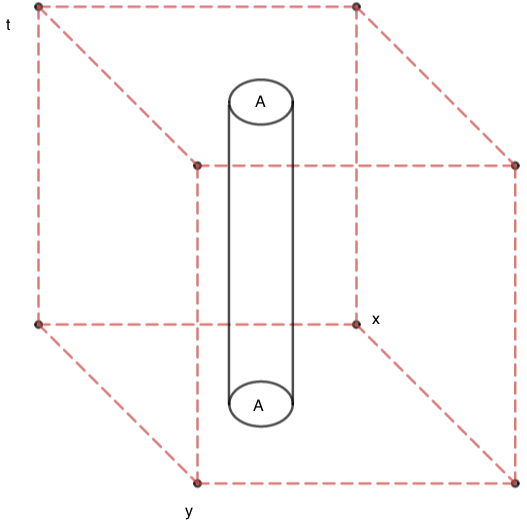
\includegraphics[scale=0.4]{10-3.png}}
    \caption{Drawing for Wangsness 10-3}
\end{figure}
\subsubsection{Wangsness 10-6}
We are given that $\mathbf{P} = P_0 \hat{\mathbf{k}}$. Now $\rho_{b} = -\nabla \cdot \mathbf{P}$, and as $\mathbf{P}$ is uniform, $-\nabla \cdot \mathbf{P} = 0$. Thus $\rho_b = 0$. $\sigma_b = \mathbf{P}\cdot \hat{\mathbf{n}} = P_0 \hat{\mathbf{k}} \cdot \hat{\mathbf{n}} = P_0 \cos(\theta)$. The positive charge is thus located in the region $\theta < \frac{\pi}{2}$. So $Q_b^+ = \int_{0}^{\pi/2}\int_{0}^{2\pi} P_0 \cos(\theta) a^2 \sin(\theta) d\theta d\phi = \pi a^2 P_0$.
\begin{figure}[htbp]
    \centering
    {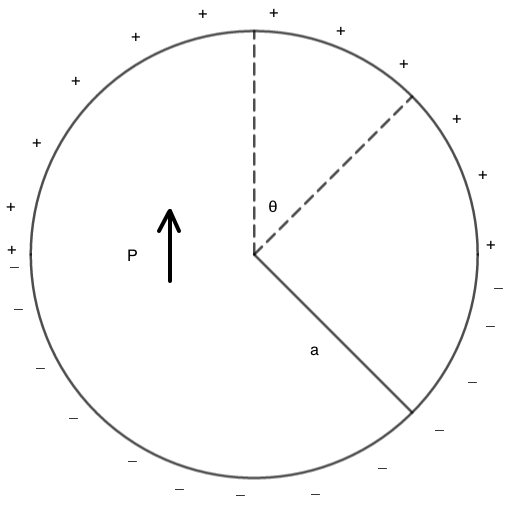
\includegraphics[scale=0.3]{10-6.png}}
    \caption{Drawing for Wangsness 10-6}
\end{figure}
\subsubsection{Wangsness 10-17}
Choose a spherical Gaussian surface outside the sphere concentric with the given sphere. $\int \mathbf{D}\cdot \mathbf{da} = Q_f$, so $D_o (4\pi r^2) = q$, and thus $\mathbf{D}_o = \frac{q}{4\pi r^2} \hat{\mathbf{r}}$. From $\mathbf{D} = \epsilon_0 \mathbf{E}+\mathbf{P}$, we have that $\mathbf{D}_o - \epsilon_0 \mathbf{E}_o = \mathbf{P}_o$. $\mathbf{E}_0 = \frac{q}{4\pi \epsilon_0 r^2}\hat{\mathbf{r}}$, and thus $\mathbf{P}_o = 0$. There is no dielectric outside of the sphere. Choosing a Gaussian surface inside of the sphere, we get $\int \mathbf{D}\cdot \mathbf{da} = Q_f$, for $D(4\pi r^2) = q$, and thus $\mathbf{D}_i = \frac{q}{4\pi r^2} \hat{\mathbf{r}}$. $\mathbf{E}_i = \frac{\mathbf{D}_i}{\epsilon} = \frac{\mathbf{D}_i}{\kappa_e \epsilon_0} = \frac{q}{4\pi \kappa_{e} \epsilon_0 r^2}\hat{\mathbf{r}}$. So $\mathbf{P}_i = \mathbf{D}_i - \epsilon_0 \mathbf{E}_i = (1-\frac{1}{\kappa_{e}}) \frac{q}{4\pi r^2} \hat{\mathbf{r}}$. Finally, $Q_b^{surface} = \int_{S} \sigma_{b} da' = \iint \mathbf{P}\cdot \hat{\mathbf{n}} da' = \int_{0}^{\pi} \int_{0}^{2\pi} \frac{\kappa_e-1}{\kappa_e} \frac{q}{4\pi} \sin(\theta) d\theta d\phi = \frac{\kappa_e-1}{\kappa_e} q$.
\subsubsection{Wangsness 10-18}
$\oint \mathbf{D} \cdot \mathbf{da} = q$. $\mathbf{D} = \frac{q}{4\pi r^2} \hat{\mathbf{r}}$ for all $r$ inside the cavity or in the dielectric. $\rho_b = 0$ since $\rho_f = 0$ in the dielectric. In the dielectric $\mathbf{E} = \frac{\mathbf{D}}{\epsilon} = \frac{\mathbf{D}}{\kappa_e \epsilon_0}$, so $\mathbf{E} = \frac{q}{4\pi \kappa_e \epsilon_0 r^2}\hat{\mathbf{r}}$. $\mathbf{P} = \mathbf{D}- \epsilon_0 \mathbf{E} = \frac{\kappa_e-1}{\kappa_e} \frac{q}{4\pi r^2} \hat{\mathbf{r}}$ at the surface of the cavity $r=a$. $\sigma_b = \mathbf{P}\cdot \hat{\mathbf{n}} = \frac{\kappa_e-1}{\kappa_e} \frac{q}{4\pi a^2} \hat{\mathbf{r}}\cdot (-\hat{\mathbf{r}}) = - \frac{\kappa_e-1}{\kappa_e} \frac{q}{4\pi a^2}$. $Q_b^{cavity} = \int \sigma da = - \frac{\kappa_e-1}{\kappa_e}q$.
\subsubsection{Wangsness 10-25}
$\kappa_e(x) = \alpha+\beta x$ (The dielectric constant varies linearly with $x$. $\alpha$ and $\beta$ are constants). Find $\mathbf{D}$ between the plates. $\int_{Gaussian Surface} \mathbf{D}\cdot \mathbf{da} = Q_f^{enc}$ (D is uniform between plates). $D\Delta a = Q_f^{enc}$, and thus $D = \frac{Q_f^{enc}}{\Delta a} = \sigma = \frac{Q}{A}$, where $Q$ is the total charge of the plate and $A$ is the area of the plate. $E = \frac{D}{\epsilon} = \frac{Q}{\kappa \epsilon_0 A} = \frac{Q}{\epsilon_0 A(\alpha + \beta x)}$. At $x=0$, $\kappa_e = \kappa_{e_1}$, so $\alpha+\beta(0) = \kappa_{e_1}$, and thus $\alpha = \kappa_{e_1}$. At $x=d$, $\kappa_{e} = \kappa_{e_2}$, and so $\beta = \frac{\kappa_{e_2}-\kappa_{e_1}}{d}$. The potential difference between the plates is $\Delta \phi = -\int_{-}^{+} \mathbf{E}\cdot \mathbf{d\ell} = \int_{+}^{-} Edx = \frac{Q}{\epsilon_0 A} \int_{0}^{d} \frac{dx}{\alpha+\beta x} = \frac{Q}{\epsilon A} \frac{1}{\beta} \ln(\alpha+\beta x)\big|_{0}^{d} = \frac{Q}{\epsilon_0 A\beta} \ln(\frac{\alpha+\beta d}{\alpha}) = \frac{Q}{\epsilon_0 A\beta} \ln(\frac{\kappa_{e_2}}{\kappa_{e_1}}) = \frac{Q}{C}$. Hence $C = \frac{\epsilon_0 A\beta}{\ln(\frac{\kappa_{e_2}}{\kappa_{e_1}})} = \frac{(\kappa_{e_2}-\kappa_{e_1})\epsilon_0 A}{d\ln(\frac{\kappa_{e_2}}{\kappa_{e_1}})}$
\begin{figure}[H]
  \begin{subfigure}[b]{0.49\textwidth}
     \centering
    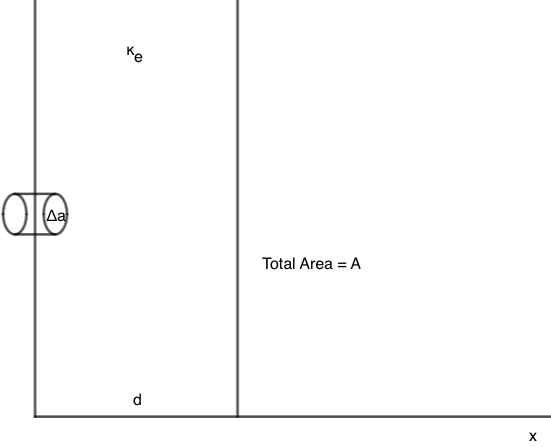
\includegraphics[width=\textwidth]{10-25.png}
    \caption{Drawing for Wangsness 10-25}
  \end{subfigure}
  \begin{subfigure}[b]{0.49\textwidth}
    \centering
    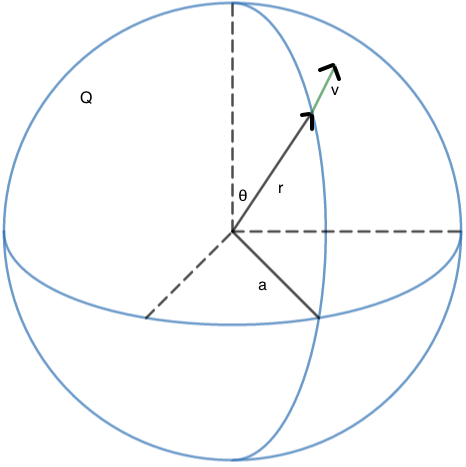
\includegraphics[width=\textwidth]{12-3.png}
    \caption{Drawing for Wangsness 12-3}
  \end{subfigure}
\end{figure}
\subsubsection{Wangsness 10-27}
$\kappa = \kappa_{e_1}$ for $a\leq \rho < \rho_0$, $\kappa = \kappa_{e_2}$ for $\rho_0 \leq \rho \leq b$. First get $D$ by assuming a charge per unit length $\lambda $on the inner cylinder and $-\lambda$ on the outer. $\int \mathbf{D}\cdot \mathbf{da} = Q_{f}^{enc} = D(2\pi \rho L) = \lambda L$. So $\mathbf{D} = \frac{\lambda}{2\pi \rho} \hat{\boldsymbol{\uprho}}$. $\Delta \phi = -\int_{-}^{+} \mathbf{E} \cdot \mathbf{d\ell} = \int_{a}^{b} \frac{\lambda}{2\pi \rho \epsilon}d\rho = \int_{a}^{\rho_0} \frac{\lambda}{2\pi \epsilon_0 \kappa_{e_1}\rho}d\rho + \int_{\rho_0}^{b} \frac{\lambda}{2\pi \epsilon_0 \kappa_{e_2}\rho}d\rho = \frac{\lambda}{2\pi \epsilon_0}\big[\frac{1}{\kappa_{e_1}}\ln(\frac{\rho_0}{a}) + \frac{1}{\kappa_{e_2}}\ln(\frac{b}{\rho_0})\big]$. From $\Delta \phi = \frac{Q}{C}$, and $Q=\lambda L$, we get $C = \frac{2\pi \epsilon_0 L}{\frac{1}{\kappa_{e_1}}\ln(\frac{\rho_0}{a}) + \frac{1}{\kappa_{e_2}}\ln(\frac{b}{\rho_0})}$
\subsection{Homework XI}
\subsubsection{Wangsness 12-3}
$\mathbf{J} = \rho \mathbf{v}$. $\rho = \frac{Q}{\frac{4}{3}\pi a^3} = \frac{3q}{4\pi a^3}$. $\mathbf{u} = \mathbf{\omega}\times\mathbf{r} = \omega \hat{\mathbf{z}} \times r \hat{\mathbf{r}} = \omega r \sin(\theta) \hat{\boldsymbol{\upvarphi}}$. So, we have that $\mathbf{J} = \frac{3Q}{4\pi a^3} \omega r \sin(\theta) \hat{\boldsymbol{\upvarphi}}$. $\mathbf{da} = rdrd\theta \hat{\boldsymbol{\upvarphi}}$, so $I = \int \mathbf{J} \cdot \mathbf{da} = \frac{3Q \omega}{4\pi a^3} \int_{0}^{\pi} \int_{0}^{a} r^2\sin(\theta)drd\theta = \frac{Q\omega}{2\pi}$
\subsubsection{Wangsness 13-4}
We will calculate the force exerted by $C'$ on $C$. $\mathbf{F}_{C'\rightarrow C} = \frac{\mu_0}{4\pi} \oint_{C} \oint_{C'} \frac{I \mathbf{d\ell}\times (I' \mathbf{d\ell}'\times \hat{\mathbf{r}})}{R^2}$. We use the $BAC-CAB$ rule: $\mathbf{A}\times(\mathbf{B}\times \mathbf{C}) = \mathbf{B}(\mathbf{A}\cdot \mathbf{C}) - \mathbf{C}(\mathbf{A}\cdot \mathbf{B})$. We can rewrite the previous integral as  $\mathbf{F}_{C'\rightarrow C} = -\frac{\mu_0 II'}{4\pi} \oint_{C} \oint_{C'} \big[ \mathbf{d\ell}'\cdot(\mathbf{d\ell}\times \frac{\hat{\mathbf{r}}}{R^2}) - \frac{\hat{\mathbf{r}}}{R^2} \mathbf{d\ell}\cdot \mathbf{d\ell}\big]$. Recall that $\nabla(\frac{1}{R}) = \frac{\hat{\mathbf{r}}}{R^2}$. Using this, we have $\mathbf{F}_{C'\rightarrow C} = -\frac{\mu_0 II'}{4\pi} \oint_{C}\oint_{C'} \mathbf{d\ell'}\big[ \mathbf{d\ell}\cdot \nabla(\frac{1}{R})- \frac{\hat{\mathbf{r}}}{R^2} \mathbf{d\ell'} \cdot \mathbf{d\ell}\big]$. From the fundamental theorem of gradients, $\oint \nabla(f) \cdot \mathbf{d\ell} = 0$ for any function $f$. Thus $\oint \nabla(\frac{1}{R}) \cdot \mathbf{d\ell} = 0$. From this we have $\mathbf{F}_{C\rightarrow C'} = -\frac{\mu_0 II'}{4\pi} \oint_{C}\oint_{C'} \frac{\hat{\mathbf{r}}}{R^2} \mathbf{d\ell}'\cdot \mathbf{d\ell}$. We now compute this integral along all four paths of the problem. $\mathbf{d\ell}' = dz' \hat{\mathbf{z}}$ for all paths. Along path $I$, $\mathbf{r} = \hat{\mathbf{x}}d+\hat{\mathbf{z}}z$, $\mathbf{d\ell} = \hat{\mathbf{z}}dz$. Along path $III$, $\mathbf{r} = \hat{\mathbf{x}}(a+d)+\hat{\mathbf{z}}z$, $\mathbf{d\ell} = \hat{\mathbf{z}}dz$. Along paths $II$ and $IV$, $\mathbf{d\ell}\cdot \mathbf{d\ell}' = 0$. Piecing this together, $\mathbf{F}_{C\rightarrow C'} = -\frac{\mu_0 II'}{4\pi}\int_{0}^{b} \int_{-\infty}^{\infty} \frac{\hat{\mathbf{x}}d+\hat{\mathbf{z}}(z-z')}{\big(d^2+(z-z')^2\big)^{3/2}}dz'dz - \frac{\mu_0 II'}{4\pi} \int_{b}^{0} \int_{-\infty}^{\infty} \frac{\hat{\mathbf{x}}(d+a)+\hat{\mathbf{z}}(z-z')}{\big((d+a)^2+(z-z')^2\big)^{3/2}}dz'dz$. Making the substitution $t=z'-z$, we get an integral of the form $\int_{-\infty}^{\infty} \frac{t+z'}{(A+t^2)^{3/2}}dt$. This is an odd function that is integrated over symmetric bounds, and thus the integral is zero. The only part left is the $\hat{\mathbf{x}}$ contribution. Evaluating this integral, we get $\mathbf{F}_{C\rightarrow C'} = -\frac{\mu_0 II' ab}{2\pi d(a+d)}\hat{\mathbf{x}}$.
\begin{figure}[htbp]
    \centering
    {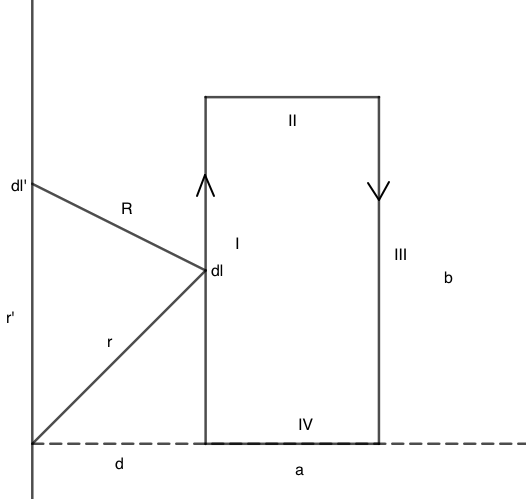
\includegraphics[scale=0.4]{13-4.png}}
    \caption{Drawing for Wangsness 13-4}
\end{figure}
\subsubsection{Wangsness 14-7}
$\mathbf{R} = \mathbf{r}-\mathbf{r}'$, where $\mathbf{r} = z\hat{\mathbf{z}}$ and $\mathbf{r}' = a\cos(\phi')\hat{\mathbf{x}}+a\sin(\phi')\hat{\mathbf{y}}$. We have $\boldsymbol{d\ell}' = ad\varphi' \hat{\boldsymbol{\upvarphi}}$. Putting this together, we have $\mathbf{R} = z\hat{\mathbf{z}} - a(\cos(\phi')\hat{\mathbf{x}}+\sin(\phi')\hat{\mathbf{y}})$. So:
\begin{align*}
    \mathbf{B} &= \frac{\mu_0 I'}{4\pi}\int \frac{\boldsymbol{d\ell}\times \mathbf{R}}{R^3} = \frac{\mu_0I'}{4\pi} \int_{-\alpha}^{\alpha} \frac{ad\phi' \hat{\boldsymbol{\upvarphi}}\times (z\hat{\mathbf{z}}-a\cos(\phi')\hat{\mathbf{x}}-a\sin(\phi')\hat{\mathbf{y}})}{(z^2+a^2)^{3/2}}\\
    &= \frac{\mu_0 I'a}{4\pi(z^2+a^2)^{3/2}}\int_{-\alpha}^{\alpha} (-\sin(\phi')\hat{\mathbf{x}}+\cos(\phi')\hat{\mathbf{y}})\times (-a\cos(\phi')\hat{\mathbf{x}}-a\sin(\phi')\hat{\mathbf{y}}+z\hat{\mathbf{z}})d\phi'\\
    &= \frac{\mu_0 I'a}{4\pi (z^2+a^2)^{3/2}}\int_{-\alpha}^{\alpha} (z\cos(\phi')\hat{\mathbf{x}}+z\sin(\phi')\hat{\mathbf{y}}+a\hat{\mathbf{z}})d\phi'
\end{align*}
Sine is an odd function, and the limit is over a symmetric interval, and thus the $\hat{\mathbf{y}}$ component is zero. So we have:
\begin{equation*}
    \mathbf{B} = \frac{\mu_0 I' a}{2\pi (z^2+a^2)^{3/2}}\big(z\sin(\alpha)\hat{\mathbf{x}}+a\alpha \hat{\mathbf{z}}\big)    
\end{equation*}
\subsubsection{Wangsness 14-15}
The force on $q$ is given by $\mathbf{F} = q\mathbf{v}\times \mathbf{B}$. We first get $\mathbf{B}$ at $q$. $\mathbf{B} = \frac{\mu_0}{4\pi} \int \frac{I' d\ell' \times \hat{\mathbf{r}}}{R^2}$. For this problem, $\mathbf{R} = -\rho' \hat{\boldsymbol{\uprho}}$. We need only compute the integral along paths $I$ and $III$, for along $II$ and $IV$ we have that $\mathbf{d\ell}$ and $\mathbf{R}$ are parallel. So, we have $\mathbf{B} = \frac{\mu_0}{4\pi} \int_{0}^{\pi} \frac{I'(-ad\phi' \hat{\boldsymbol{\upvarphi}})\times (-a\hat{\boldsymbol{\uprho}})}{a^3}+ \frac{\mu_0}{4\pi} \int_{0}^{\pi} \frac{I'(bd\phi' \hat{\boldsymbol{\upvarphi}})\times (-b\hat{\boldsymbol{\uprho}})}{b^3} = \frac{\mu_0 I'}{4} \frac{b-a}{ab} \hat{\mathbf{z}}$. The force is $\mathbf{F} = qv\hat{\mathbf{y}} \times \frac{\mu_0 I}{4} \frac{b-a}{ab} \hat{\mathbf{z}} = \frac{qv\mu_0 I'}{4} \frac{b-a}{ab} \hat{\mathbf{x}}$
\begin{figure}[htbp]
    \centering
    {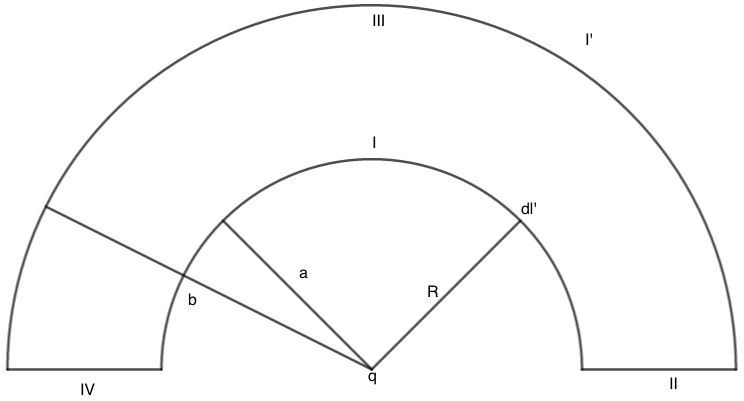
\includegraphics[scale=0.4]{14-15.png}}
    \caption{Drawing for Wangsness 14-15}
\end{figure}
\subsection{Homework XII}
\subsubsection{Wangsness 15-7}
For $\rho\leq a$, path $(1)$ has $\oint \mathbf{B}\cdot \mathbf{d\ell}= \mu_0 I_{enc}$, where $I_{enc} = I\frac{\rho^2}{a^2}$. So $\mathbf{B} = \frac{\mu_0 I\rho}{2\pi a^2} \hat{\boldsymbol{\upvarphi}}$. For $a\leq \rho \leq b$, $I_{enc} = I$. So $B = \frac{\mu_0 I}{2\pi \rho} \hat{\boldsymbol{\upvarphi}}$. For $b\leq \rho \leq c$, $I_{enc} = I =I\frac{\rho^2-b^2}{c^2-b^2} = I\frac{c^2-\rho^2}{c^2-b^2}$. So $\mathbf{B} = \frac{\mu_0 I}{2\pi \rho} \frac{c^2-\rho^2}{c^2-b^2}\hat{\boldsymbol{\upvarphi}}$. FInally, or $\rho \geq c$, $I_{enc} = 0$, so $\mathbf{B} = 0$.
\begin{figure}[htbp]
    \centering
    {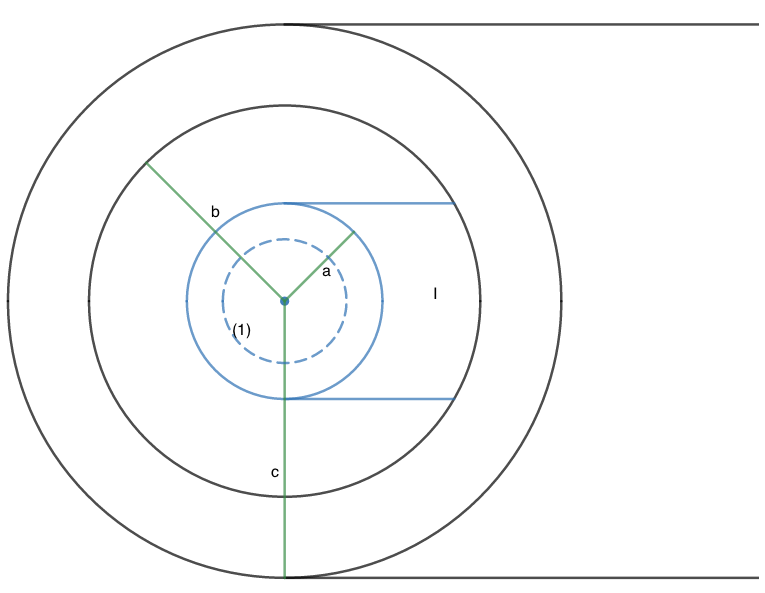
\includegraphics[scale=0.4]{15-7.png}}
    \caption{Drawing for Wangsness 15-7}
\end{figure}
\subsubsection{Wangsness 15-8}
\begin{equation*}
    \mathbf{B} = \begin{cases} 0, & \rho < a \\ \frac{\mu_0 I}{2\pi \rho}\frac{\rho^2-a^2}{b^2-a^2}\hat{\boldsymbol{\upvarphi}}, & a<\rho < b \\ \frac{\mu_0 I}{2\pi \rho} \hat{\boldsymbol{\upvarphi}}, & \rho>b\end{cases}    
\end{equation*}
By definition, $\mu_0 \mathbf{J} = \nabla \times \mathbf{B}$. So:
\begin{equation*}
    \mathbf{J} = \begin{cases} 0, & \rho<a\\ \frac{I}{\pi(b^2-a^2)}, & a<\rho < b\\ 0, & \rho>b \end{cases}    
\end{equation*}
The current $I$ i distributed uniformly over the volume between two coaxial cylinders of inner radius $a$ and outer radius $b$ in the direction of the cylinder axis.
\subsubsection{Wangsness 16-10}
The field point is on the $z-$axis. $\mathbf{r} = z\hat{\mathbf{z}}$, $\mathbf{r}' =  a\cos(\phi')\hat{\mathbf{x}}+a\sin(\phi')\hat{\mathbf{y}}$. $\mathbf{d\ell}' = \mathbf{dr}' = ad\phi' \hat{\boldsymbol{\upvarphi}} = ad\phi' (-\sin(\phi')\hat{\mathbf{x}}+\cos(\phi')\hat{\mathbf{y}})$. $\mathbf{A} = \frac{\mu_0 I'}{4\pi} \int \frac{\mathbf{d\ell}'}{R} = \frac{\mu_0 I'}{4\pi} \frac{a}{\sqrt{a^2+z^2}}\int_{-\alpha}^{\alpha} (-\sin(\phi')\hat{\mathbf{x}}+\cos(\phi')\hat{\mathbf{y}})d\phi' = \frac{\mu_0 I'a}{2\pi \sqrt{a^2+z^2}}\sin(\alpha)\hat{\mathbf{y}}$. To find $\mathbf{B}$ from $\mathbf{A}$, we need to evaluate $\nabla \times \mathbf{A}$. We don't know about $\mathbf{A}$ for a general point, and thus we can't evaluate the $x$ and $y$ derivatives.
\subsection{Homework XIII}
\subsubsection{Wangsness 17-3}
The $\mathbf{B}$ field associated with $I$ is $\mathbf{B} = \frac{\mu_0 I}{2\pi \rho} \hat{\boldsymbol{\upvarphi}}$. In the plane of the paper, $\phi$ is into the paper. $\Phi = \int \mathbf{B}\cdot \mathbf{da} = \int \frac{\mu_0 I}{2\pi \rho} \cdot b d\rho \hat{\boldsymbol{\upvarphi}} = \frac{\mu_0Ib}{2\pi} \int_{d}^{d+a} \frac{d\rho}{\rho}= \frac{\mu_0 Ib}{2\pi} \ln(\frac{d+a}{d}) = \frac{\mu_0 bI_0 e^{-\lambda t}}{2\pi} \ln(\frac{d+a}{d}) = \frac{\mu_0 I_0 \lambda b}{2\pi} \ln(\frac{d+a}{d})e^{-\lambda t}$. The induced current is clockwise around the loop to produce a field which goes into the paper to counteract the decreasing $\mathbf{B}$ due to $I_0$.
\subsubsection{Wangsness 17-4}
The $\mathbf{B}-$field at distance $\rho$ from the wire at points in the plane of the paper is $\mathbf{B} = \frac{\mu_0 I}{2\pi \rho} \hat{\mathbf{y}}$. The flux of $\mathbf{B}$ through the loop is $\Phi = \int \mathbf{B}\cdot \mathbf{da} = \iint \frac{\mu_0 I}{2\pi \rho}\rho d\theta d\rho$. We have $\rho = b+r\cos(\theta)$. So $\Phi = \frac{\mu_0 I}{2\pi} \int_{0}^{a} \int_{0}^{2\pi} \frac{r d\theta dr}{b+r\cos(\theta)} = \frac{\mu_0 I}{2\pi} \int_{0}^{a} \frac{2r}{\sqrt{b^2-r^2}}\tan^{-1}\big[\frac{\sqrt{b^2-r^2}\tan(\theta/2)}{b+r}\big]_{0}^{2\pi} \Rightarrow \tan^{-1}\big[\frac{\sqrt{b^2-r^2}}{b+r}\tan(\pi)\big] - \tan^{-1}\big[ \frac{\sqrt{b^2-r^2}}{b+r}\tan(0)\big]$. So $\Phi = \mu_0 I\big[b-\sqrt{b^2-a^2}\big]$. The loop moves with constant speed $v$ along the $x-$axis away from the current $I$, $v = \frac{db}{dt}$. So $\xi = -\frac{d\Phi}{dt} = -\mu_0 I \frac{d}{dt}\big[b-\sqrt{b^2-a^2}\big] = -\mu_0 I\big[ v-\frac{bv}{\sqrt{b^2-a^2}}\big] = \mu_0 NIv\big[ \frac{b}{\sqrt{b^2-a^2}}-1\big]$. The current will be clockwise trying to increase the flux which is decreasing due to motion away from the wire.
\begin{figure}[htbp]
    \centering
    {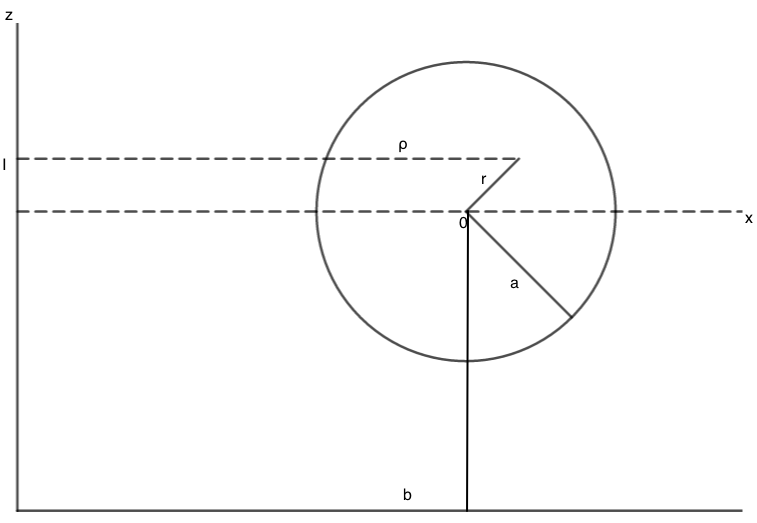
\includegraphics[scale=0.4]{17-4.png}}
    \caption{Drawing for Wangness 17-4}
\end{figure}
\subsubsection{Wangsness 17-19}
$\Phi_{12} = IM_{12}$. The flux due to $1$ through $2$ is $\Phi_{12} = \int \mathbf{B}_1 \cdot \mathbf{da}_2$. $\mathbf{B}_1 = \frac{\mu_0 I}{2\pi} \big( \frac{1}{\rho+d}- \frac{1}{\rho+d+D}\big)$. So we have that $\Phi_{12} = \int_{0}^{a} \frac{\mu_0 I}{2\pi} \big(\frac{1}{\rho+d}- \frac{1}{\rho+d+D}\big) bd\rho = \frac{\mu_0 Ib}{2\pi}\big[ \ln(\frac{a+d}{a+d+D}) - \ln(\frac{d}{d+D})\big]$. Thus, we have $M = \frac{\mu_0 b}{2\pi} \ln\big(\frac{a+d}{d}\big)$
\subsubsection{Wangsness 17-20}
The field inside the toroid is $\mathbf{B} = \frac{\mu_0 NI}{2\pi \rho} \hat{\boldsymbol{\upvarphi}}$. The flux through a single turn is $\Phi^1 = \frac{\mu_0 NI}{2\pi} \int_{0}^{a} \int_{0}^{2\pi} \frac{r}{b+r\cos(\theta)}d\theta dr$. We've done this integral before, and we get $\Phi^1= \mu_0 NI\big[b-\sqrt{b^2-r^2}\big]$. $\Phi = N\Phi^1$. $L = \frac{\Phi}{I} = \frac{\mu_0 N^2 I}{I} \big[b-\sqrt{b^2-r^2}\big] = \mu_0 N^2 \big[b-\sqrt{b^2-r^2}\big]$
\section{Exams}
\subsection{Exam I}
\subsubsection{Question I}
Give the vector field field $\mathbf{A} = c\hat{\boldsymbol{\uptheta}}$, where $c$ is a constant, find $\nabla \times \mathbf{A}$. Is this a conservative vector field? Explain.
\subsubsection{Question II}
Verify the Divergence Theorem for $\mathbf{A}$ given in problem 1 in spherical coordinates for a hemisphere of radius $a_0$ resting on the $xy-plane$ with the center of the flat base of the hemisphere at the origin and the symmetry axis of the hemisphere along the positive $z-axis$.
\subsubsection{Question III}
A semicircular charged line of radius $a$ carries uniform linear charge density $\lambda$. It has the equation $x^2+y^2 = a^2$, $x\geq 0$, $z=0$. That is, the half circle resting on the $xy-plane$ of radius $a$. Find the electring field at a point $P$ on the $z$ axis a distance $z$ from the origin.
\subsection{Exam II}
\subsubsection{Question I}
A conducting sphere of radius $a$, centered at the origin carries charge $Q_1$. This sphere is surrounded by a hollow concentric conducting spherical shell of inner radius $b$ and outer radius $c$ with $a<b<c$. The outer hollow conducting shell caries a total charge $Q_2$. 
\begin{enumerate}
    \item What is the electric field everywhere?
    \item What is the potential everywhere, assuming $\underset{r\rightarrow \infty} \lim \phi(r) = 0$?
    \item How much charge is on the inner and outer surfaces of the conducting shell at $r=b$ and $r=c$?
\end{enumerate}
\subsubsection{Question II}
The outer conductor of problem I is now grounded.
\begin{enumerate}
    \item What is the electric field everywhere?
    \item What is the potential everywhere?
    \item How much charge is on the surfaces at $r=b$ and $r=c$?
    \item What is the capacitance of the system of conductors?
    \item Calculate the electrostatic potential energy of the configuration assuming the energy resides in the charges.
    \item Calculate the electrostatic potential energy of the configuration assuming the energy resides in the electric field.
\end{enumerate}
\subsubsection{Question III}
A semicircular arc of radius $a$ in the $y-z$ plane with center on the $y-axis$ at the origin and the top of the arc on the positive $y-axis$ carries linear charge density $\lambda = \lambda_0 \cos(\theta')$, where $\lambda_0$ is constant and $\theta'$ is measured with respected to the positive $z-axis$.
\begin{enumerate}
    \item What is the electric monopole moment of this distribution?
    \item What is the electric dipole moment of this distribution?
    \item What is the electric potential at a distance $r$ from the origin for this distribution where $r>a$, accurate to order $\frac{1}{r^2}$?
\end{enumerate}
\subsection{Exam III}
\subsubsection{Question I}
The electric field in a spherical region of space of radius $a$ is given by $\mathbf{E} = E_0 \frac{r^2}{a^2}\hat{\mathbf{r}}$ for $r< a$, where $E_0$ is a constant. This region is surrounded concentrically by a grounded conducting spherical shell of inner radius $b$ and outer radius $c$ with $a<b<c$. There is no charge in the region $a<r<b$. 
\begin{enumerate}
    \item What is the electric charge density in the region $r<a$?
    \item Wher is the electric field in the region $a<r<b$?
    \item How much charge is on the surfaces at $r=b$ and $r=c$?
    \item What is the electric field for $r>c$?
    \item What is the electric potential $\phi$ at $r=0$ assuming that ground potential is $\phi = 0$.
\end{enumerate}
\subsubsection{Question II}
A capacitor $C_{1}$ is charged to a potential difference $\Delta \phi$ between its plates. A second capacitor $C_{2}$ is uncharged. One plate of $C_2$ is now connected to a plate of $C_1$ by a conductor of negligible capacitance, the remaining plates are similarly connected. 
\begin{enumerate}
    \item For the resultant equilibrium state, find the charge on each capacitor and the potential difference $\Delta \phi$ between their respective plates.
    \item Compare the energy stored in capacitor $C_1$ before connecting it to $C_2$, to the energy of the combination after connected them. Are these energies the same? If not, which is larger and where did any additional energy come from, or where did any lost energy go?
\end{enumerate}
\subsubsection{Question III}
Find the electric dipole moment of an hourglass configuration of charge consisting of two identical right circular cones of radius $a$ and height $a$ with symmetry axes aligned apex to apex along the $z-$axis with the apexes touching at the origin. The top cone has charge density $\sigma_0$ on its surface, and the bottom cone has charge density $-\sigma_0$ on its surface.
\subsection{Practice Final Exam}
\subsubsection{Problem I}
The electric field in a region of space is given in spherical coordinates as $\mathbf{E} = cr\hat{\mathbf{r}}$, where $c$ is constant. 
\begin{enumerate}
    \item Find the charge density at a point $(r,\theta,\phi)$
    \item Find the total charge inside a sphere of radius $a$ centered at the origin.
\end{enumerate}
\subsubsection{Problem II}
A battery is used to charge an ideal parallel plate capacitor to a potential difference $\Delta \phi = V_0$. The battery is then disconnected. The separation between the plates is now increasing from $d$ to $\alpha d$, where $\alpha >1$. The area of the plates is $A$.
\begin{enumerate}
    \item What is the ratio of the new energy to the original energy>
    \item Is the energy increases or decreased?
    \item Where does this energy come from or go to?
    \item Compute the change in energy $\Delta U_e$ expressing your answer in terms of the given quantities $V_0,d,A,\alpha$ and fundamental constants.
\end{enumerate}
\subsubsection{Problem III}
A dielectric sphere of radius $a$ and permittivity $\varepsilon$ contains a free charge density. $\rho_f = cr$, where $c$ is a constant. The sphere is centered at the origin. Find the electric potential at the center of the sphere assuming that the potential is zero at an infinite distance from the center.
\subsubsection{Problem IV}
A thick slab extending from $z=-a$ to $z=a$ carries a uniform vlume current density $\mathbf{J} = J_0 \hat{\mathbf{x}}$. The slab is infinite in the $xy-$plane. Find the magnetic field $B$ as a function of $z$ inside and outside the slab. Plot $B$ as a function of $z$ for $-b<z<b$ where $b>a$.
\subsubsection{Problem V}
An ideal long solenoid of radius $a$, carrying $n$ turns per unit length, is looped by a wire with resistance $R$. 
\begin{enumerate}
    \item If the current in the solenoid is increasing at a constant rate $\frac{dI}{dt} = k$, what current flows in the lopp, and which way (Left or right) does it pass through the resistor?
    \item If the current $I$ in the solenoid is constant but the solenoid is pulled out of the loop and reinserted in the opposite direction, what total charge passes through the resistor?
\end{enumerate}
\subsection{Final Exam}
\subsubsection{Problem I}
\begin{enumerate}
    \item Write down Maxwell's Equations in differential form.
    \item Convert them to integral form and show derivations.
    \item Name each equation.
\end{enumerate}
\begin{proof}[Solution]
\
\begin{enumerate}
\item Gauss' Law: $\nabla \cdot \mathbf{E} = \frac{\rho}{\epsilon_0}\Rightarrow\frac{Q_{encl}}{\epsilon_0}=\iiint_{V} \frac{\rho}{\epsilon_0}d\tau=\iiint_{V} \big(\nabla \cdot \mathbf{E}\big) d\tau = \oiint_{\partial V} \mathbf{E}\cdot \mathbf{da}$
\item Faraday's Law: $\nabla \times \mathbf{E} = -\frac{\partial \mathbf{B}}{\partial t}\Rightarrow-\frac{d \Phi_{B}}{dt} = \iint_{S} -\frac{\partial \mathbf{B}}{\partial t}da = \iint_{S} \big(\nabla \times \mathbf{E}\big)da = \oint_{\partial S}\mathbf{E}\cdot \mathbf{d\ell}$
\item Gauss' Law of Magnetism: $\nabla \cdot \mathbf{B} = 0\Rightarrow 0 = \iiint_{V} \big(\nabla \cdot\mathbf{B}\big)d\tau = \oiint_{\partial V} \mathbf{B}\cdot \mathbf{da}$
\item Ampere's Law: $\nabla \times \mathbf{B} = \mu_0 \mathbf{J} + \mu_0 \epsilon_0 \frac{\partial \mathbf{E}}{\partial t}\Rightarrow\mu_0 I_{encl}+ \mu_0 \epsilon_0 \frac{d\Phi_{E}}{dt} = \iint_{S}\big(\mu_0 \mathbf{J} + \mu_0 \epsilon_0 \frac{\partial \mathbf{E}}{\partial t}\big)da = \iint_{S}\big(\nabla \times \mathbf{B}\big)da = \oint_{\partial S}\mathbf{B}\cdot \mathbf{d\ell}$
\end{enumerate}
\end{proof}
\subsubsection{Problem II}
A conduction sphere of radius $a$ carries a charge $Q_{1}$. It is surrounded by a conducting spherical shell of inner radius $b$ and outer radius $c$ with $a<b<c$. The charge on the conducting shell is $Q_{2}$. The region between the conductors $a<r<b$ is filled with linear isotropic dielectric of permittivity $\varepsilon$. Find the following in the regions $r<a.a<r<b.b<r.b<r<c.c<r$:
\begin{enumerate}
    \item The electric displacement $\mathbf{D}$
    \item The electric field $\mathbf{E}$
    \item The polarization vector $\mathbf{P}$
    \item Find the free charge on the conductors at $r=a,b,c$.
    \item The bound volume charge in the dielectric.
    \item The bound surface charge density at the inner and outer surfaces of the dielectric.
    \item The electric potential at the origin assuming the potential is zero as $r$ goes to infinity.
\end{enumerate}
\begin{proof}[Solution]
\
\begin{enumerate}
\begin{multicols}{2}
    \item $\mathbf{D}=\begin{cases}\mathbf{0}&r<a\\ \frac{Q_{1}}{4\pi r^{2}} &a<r<b\\\mathbf{0} & b<r<c\\ \frac{Q_{1}+Q_{2}}{4\pi r^{2}} & c<r \end{cases}$
    \item $\mathbf{E}=\begin{cases}\mathbf{0}&r<a\\ \frac{Q_{1}}{4\pi\epsilon_{0} r^{2}} & a<r<b\\ \mathbf{0} & b<r<c\\ \frac{Q_{1}+Q_{2}}{4\pi\epsilon_{0}r^{2}} & c<r\end{cases}$
    \item $\mathbf{P}=\begin{cases}\mathbf{0}&r<a\\ \frac{Q_{1}}{4\pi r^{2}}(1-\frac{\epsilon_{0}}{\varepsilon}) & a<r<b\\ \mathbf{0} & b<r<c\\ \mathbf{0} & c<r \end{cases}$
    \item $Q = \begin{cases} Q_1 & r=a\\ -Q_1 & r=b\\ Q_1+Q_2 & r=c\end{cases}$
\end{multicols}
\begin{multicols}{2}
    \item $\rho_b = \nabla \cdot \mathbf{P}$, $\rho_b = 0$.
    \item $\sigma_{b,a}=-\frac{Q_1}{4\pi a^2}\big(1-\frac{\epsilon_0}{\varepsilon}\big)$, $\sigma_{b,b}=\frac{Q_1}{4\pi b^2}\big(1-\frac{\epsilon_0}{\varepsilon}\big)$.
    \end{multicols}
    \item $\phi = -\int_{0}^{\infty}\mathbf{E}\cdot \mathbf{d\ell} = \int_{c}^{\infty} \mathbf{E}\cdot \mathbf{d\ell}+\int_{b}^{c}\mathbf{E}\cdot \mathbf{d\ell}+\int_{a}^{b}\mathbf{E}\cdot \mathbf{d\ell} + \int_{0}^{a} \mathbf{E}\cdot \mathbf{d\ell} = \frac{Q_1+Q_2}{4\pi \epsilon_0 c}+\frac{Q_1}{4\pi \epsilon_0 a}-\frac{Q_1}{4\pi \epsilon_0 b}$.
\end{enumerate}
\end{proof}
\subsubsection{Problem III}
A sphere of radius $a$ carries charge density $\rho = \rho_0(r/a)$, where $\rho_0$ is a constant. Find the work done to assemble the charge distribution.
\begin{proof}[Solution]
We find $\mathbf{E}$ inside and outside using Gauss' law.
\begin{equation*}
\oiint_{S} \mathbf{E}\cdot \mathbf{da} = \frac{Q_{encl}}{\epsilon_0} = \int_{0}^{r}\int_{0}^{\pi} \int_{0}^{2\pi} \rho_0 \frac{r}{a}r^2\sin(\theta)d\varphi d\theta dr = \frac{4\pi \rho_0}{a \epsilon_0}\frac{r^4}{4} = E(4\pi r^2).
\end{equation*}
So $\mathbf{E} = \frac{\rho_0 r^2}{4a\epsilon_0}\hat{\mathbf{r}}$. Outside we have $\oiint_{S} \mathbf{E}\cdot \mathbf{da} = \int_{0}^{2\pi}\int_{0}^{\pi} \int_{0}^{a} \rho \frac{r}{a}r^2 \sin(\theta) dr d\theta d\varphi$, so $\mathbf{E} = \frac{\rho_0 a^3}{4r^2 \epsilon_0}\hat{\mathbf{r}}$. The work is
\begin{align*}
\frac{\epsilon_0}{2}\int_{All\ Space}E^2 d\tau &= \frac{\epsilon_0}{2}\int_{0}^{2\pi}\int_{0}^{\pi}\int_{0}^{\infty} E^2 r^2\sin(\theta) drd\theta d\varphi\\
&= \int_{0}^{2\pi}\int_{0}^{\pi}\int_{0}^{a} E^2r^2\sin(\theta)dr d\theta d\varphi + \int_{0}^{2\pi}\int_{0}^{\pi}\int_{a}^{\infty} E^2r^2\sin(\theta)drd\theta d\varphi\\
&= \frac{\pi \rho_0^2 a^5}{7\epsilon_0}
\end{align*}
So $\mathbf{E} = \frac{\rho_0 r^2}{4a\epsilon_0}\hat{\mathbf{r}}$
\end{proof}
\subsubsection{Problem IV}
\begin{enumerate}
    \item Could the vector field $\mathbf{F} = ax\hat{\mathbf{x}}+by\hat{\mathbf{y}}+cz\hat{\mathbf{z}}$ be a possible magnetic field, where $a+b+c\ne 0$? Explain why or why not.
    \item An electric field is given by $\mathbf{E} = ax\hat{\mathbf{y}}$, where $a$ is a constant. Is this a conservative field? Explain why or why not.
    \item Find the possible magnetic field $\mathbf{B}$ associated to $\mathbf{E}$. 
\end{enumerate}
\begin{proof}[Solution]
\
\begin{enumerate}
    \item No, for $\nabla \cdot \mathbf{F} = a+b+c \ne 0$, and therefore $\mathbf{F}$ cannot be a magnetic field.
    \item No, for $\nabla \times \mathbf{E} = a\hat{\mathbf{z}} \ne 0$, and thus $\mathbf{E}$ is not a conservative field.
    \item $\nabla \times \mathbf{E} = -\frac{\partial \mathbf{B}}{\partial t} = a\hat{\mathbf{z}}$, so $\mathbf{B} = -at\hat{\mathbf{z}}+\mathbf{B}_0$, where $\mathbf{B}_0$ is some constant vector. Here $\mathbf{B}$ is increasing with time in the $-z$ direction.
\end{enumerate}
\end{proof}
\subsubsection{Problem V}
Two infinitely long coaxial cylindrical infinitesimally thin conducting shells concentric with the $z-$axis carry oppositely directed currents of equal magnitude in the $+$ and $-$ $z-$directions. The radius of the inner shell is $a$ and that of the outer shell is $b$. What is the self-inductance of a length $\ell$ of this system?
\begin{proof}[Solution]
The flux carried by the inner shell cuts through the area of a rectangle of lenght $\ell$ and width $b-a$. So $\Phi = \int \mathbf{B}\cdot \mathbf{da} = \int_{a}^{b} \frac{\mu_0 I}{2\pi \rho}\ell d\rho = \frac{\mu_0 I\ell}{2\pi}\ln\big(\frac{b}{a}\big)$. So, $L = \frac{\Phi}{I} = \frac{\mu_0 \ell}{2\pi}\ln\big(\frac{b}{a}\big)$.
\end{proof}
\chapter{Electromagnetism II}
\section{Homework}
\subsection{Homework I}
\chapter{Mechanics}
\section{Some Notes on Lagrangian Mechanics}
The Lagrangian is defined as $\mathcal{L} = T-V$, where $T$ is the kinetic energy and $V$ is the potential energy. Hamilton's Principle, which we take upon as an axiom of nature, states that the action, $\int_{t_1}^{t_2} \mathcal{L}(x,\dot{x},t)dt$, is an extremum. This means that $\mathcal{L}$ satisfies the Euler-Lagrange equation:
\begin{equation} 
\nonumber \frac{\partial \mathcal{L}}{\partial x} - \frac{d}{dt}\big(\frac{\partial \mathcal{L}}{\partial \dot{q}}\big) = 0
\end{equation}
This is the equation of motion in a one-dimensional Cartesian system. We may use a generalized coordinate system to obtain:
\begin{equation}
\nonumber \frac{\partial \mathcal{L}}{\partial q} - \frac{d}{dt} \big(\frac{\partial \mathcal{L}}{\partial \dot{q}}\big) = 0.
\end{equation}
Let's suppose we have a nice "Physics I," style Lagrangian. By that I mean that $T = T(t)$, and $V \ne V(t)$. That is, the potential energy is a function of position, and not of time. Then the equation of motion simplifies to $\frac{\partial}{\partial q}(T-V) - \frac{d}{dt}\big(\frac{\partial}{\partial \dot{q}}(T-V)\big) = 0$, where $\frac{\partial T}{\partial q} = 0$, $\frac{\partial V}{\partial \dot{q}} = 0$, and therefore $\frac{\partial V}{\partial q} + \frac{d}{dt}\big(\frac{\partial T}{\partial \dot{q}}\big) = 0$. In a standard problem, $T = \frac{1}{2}m \dot{q}^2$. This is the kinetic energy one would find in such a "Physics I," problem. So we have that:
\begin{equation}
\nonumber m\ddot{q} = -\frac{\partial V}{\partial q}
\end{equation}
Recall that Newton's Second Law says that $m\ddot{x} = -\frac{\partial V}{\partial x}$. So this final result looks very much like Newton's Second law, except that $"x"$ is replaced with $"q"$. So, we defined the following:
\begin{definition}
The Generalized Momentum of a system is defined as $\frac{\partial \mathcal{L}}{\partial \dot{q}}$. The Generalized Force of a system is defined as $\frac{\partial \mathcal{L}}{\partial q}$.
\end{definition}
When $\mathcal{L}$ is the nice "Physics I," Lagrangian that we're familiar with, we see that Newton's Second Law appears. That is, the time derivative of momentum is equal to minus the gradient of the potential energy. For any Lagrangian, if we we generalized momentum and generalized force, then the mathematics becomes very similar to Newton's Second Law. We obtain the "Generalized," Newton's Second Law:
\begin{equation}
\nonumber Generalized\ Force = \frac{d}{dt}\big(Generalized\ Momentum\big)
\end{equation}
Let's consider the example $q = \theta$. That is, our generalized coordinate is the angle made between the particle and the $x-$axis. The generalized momentum is just angular momentum, and the generalized force is angular force (Also known as torque). Let's consider a system where $\frac{\partial \mathcal{L}}{\partial \theta} = mr^2 \ddot{\theta}$. This is particle going around in a circle. Then we have from the equation of motion that $\frac{d}{dt}\big(\frac{\partial \mathcal{L}}{\partial \dot{\theta}}\big) = mr^2 \ddot{\theta}$, and thus $\frac{\partial \mathcal{L}}{\partial \dot{\theta}} = mr^2\dot{\theta} +c$. So we arrive at $\mathcal{L} = \frac{1}{2}mr^2\dot{\theta} + g(\theta) + c\dot{\theta}$. Remember from calculus that since $\frac{\partial g(\theta)}{\partial \dot{\theta}} = 0$, we get a function of integration, and not a constant of integration. This function of integration is the $g(\theta)$ we have written down. Let's further add the requirement that $\ddot{\theta} = 0$. That is, there is no angular acceleration. This represent a particle going around in a circle at constant angular velocity. With this information, we can determine $g(\theta)$. We have that $\frac{\partial \mathcal{L}}{\partial \theta} = 0$, and thus $g'(\theta) = 0$, which means $g(\theta)$ is a constant. The Lagrangian of this problem is $\mathcal{L} = \frac{1}{2}mr^2 \dot{\theta}^2+ c_1 \dot{\theta}+c_2$. Now what of the generalized momentum? We have that $\frac{d}{dt}\big(\frac{\partial \mathcal{L}}{\partial \dot{\theta}}\big) = \frac{\partial \mathcal{L}}{\partial \theta} = 0$, and therefore $\frac{\partial \mathcal{L}}{\partial \dot{\theta}} = constant$. But our generalized momentum is simply the angular momentum. That is, we have shown that angular momentum is conserved.
\chapter{Mathematical Physics}
\section{Cheat Sheet}
\subsection{Series}
\begin{theorem*}[The Comparison Test]
If $a_n$ and $b_n$ are sequences of non-negative real numbers, if there is an $N_0\in \mathbb{N}$ such that for all $n>N_0$, $a_n\leq b_n$, and if $\sum_{n=0}^{N}b_n$ converges, then $\sum_{n=0}^{N}a_n$ converges.
\end{theorem*}
\begin{proof}
Let $B_N = \sum_{n=0}^{N}b_n$. As $b_n$ is a sequence of non-negative real numbers, $B_{N}\leq B_{N+1}$. But $B_{N}$ converges to a limit, say $B$. But then for all $N\in \mathbb{N}$, $B_{N} \leq B$. But there is an $N_{0}\in \mathbb{N}$ such that for all $n>N_{0}$, $a_n\leq b_n$. Let $S = \sum_{n=0}^{N_{0}-1}a_n$. Then $\sum_{n=0}^{N}a_n = S+\sum_{n=N_{0}}^{N}a_n \leq S+\sum_{n=N_{0}}^{N}b_n \leq S+B_{N} \leq S+B$. That is, $\sum_{n=0}^{N}a_n$ bounded by $S+B$. And as $a_n$ is non-negative, $\sum_{n=0}^{N}a_n$ increasing monotonically. But then $\sum_{n=0}^{N}a_n$ is a monotonically increases sequence that is bounded above, and therefore converges. That is, $\sum_{n=0}^{N}a_n$ converges.
\end{proof}
\begin{theorem*}[Geometric Series Theorem]
If $r$ is a real number, then
\begin{equation}
    \nonumber \sum_{n=0}^{N} r^n = \frac{1-r^{N+1}}{1-r}
\end{equation}
If $|r|<1$, then
\begin{equation}
    \nonumber \textrm{If $|r|<1$, then } \sum_{n=0}^{\infty} r^n = \frac{1}{1-r}
\end{equation}
\end{theorem*}
\begin{proof}
By induction. The base case is $1+r = (1+r)\frac{1-r}{1-r} = \frac{1-r^2}{1-r}$. Suppose it is true for $N \in \mathbb{N}$. Then $\sum_{n=0}^{N+1}r^n = \sum_{n=0}^{N}r^n + r^{N+1}$. But by induction, $\sum_{n=0}^{N}r^n = \frac{1 - r^{N+1}}{1-r}$. So $\sum_{n=0}^{N+1}r^n = \frac{1-r^{N+1}}{1-r} + r^{N+1} = \frac{1-r^{N+1} + r^{N+1}(1-r)}{1-r} = \frac{1 - r^{N+2}}{1-r}$. This completes the proof. If $|r|<1$, then $r^{N+1} \rightarrow 0$, and therefore $\underset{N \rightarrow \infty}\lim \sum_{n=0}^{N}r^n = \underset{N\rightarrow \infty}\lim \frac{1-r^{N+1}}{1-r} = \frac{1}{1-r}$.
\end{proof}

\begin{theorem*}[The Root Test Theorem]
If $a_n$ is a sequence of positive real numbers, and if $\underset{n\rightarrow \infty}\lim \sqrt[n]{a_n}<1$, then $\sum_{n=0}^{\infty} a_n$ converges, and if $\underset{n\rightarrow \infty}\lim \sqrt[n]{a_n} >1$, then $\sum_{n=0}^{\infty}a_n$ diverges.
\end{theorem*}
\begin{proof}
For if $\underset{n\rightarrow \infty}{\lim}\sqrt[n]{a_n}<1$, then there is a $c\in [0,1)$ and an $N\in \mathbb{N}$ such that for all $n>N$, $\sqrt[n]{a_n}<c$. But then $a_n< c^n$. But $|c|<1$, so $\sum_{n=0}^{\infty}c^n = \frac{1}{1-c}$. Thus, by the comparison test, $\sum_{n=0}^{N}a_n$ converges.
\end{proof}

\begin{theorem*}
There exists sequences of positive real numbers $a_n$ such that $\sqrt[n]{a_n} \rightarrow 1$, and $\sum_{n=1}^{N} a_n$ diverges.
\end{theorem*}

\begin{proof}
Let $a_n = \frac{1}{n}$. Then $\ln(\sqrt[n]{a_n}) = \frac{\ln(\frac{1}{n})}{n} = -\frac{\ln(n)}{n} \rightarrow 0$. So $\sqrt[n]{a_n} \rightarrow 1$. But $\sum_{n=1}^{N} \frac{1}{N}$ diverges.
\end{proof}

\begin{theorem*}
There exists sequences of positive real numbers $a_n$ such that $\sqrt[n]{a_n} \rightarrow 1$ and $\sum_{n=1}^{N}a_n$ converges.
\end{theorem*}
\begin{proof}
For let $a_n = \frac{1}{n^2}$. Then $\ln(\sqrt[n]{a_n}) = \frac{\ln(\frac{1}{n^2})}{n} = -2\frac{\ln(n)}{n} \rightarrow 0$. Therefore $\sqrt[n]{a_n}\rightarrow 1$. But $\sum_{n=1}^{N}\frac{1}{n^2}$ converges.
\end{proof}

\begin{theorem*}
If $a_n$ is a sequences of positive real numbers, and if $a(x)$ is a monotonically decreasing function such that for all $n\in \mathbb{N}$, $a(n) = a_n$, then $\sum_{n=1}^{\infty} a_n$ converges if and only if $\int_{1}^{\infty} a(x)dx$ converges.
\end{theorem*}
\begin{proof}
For as $a(x)$ is decreasing, for all $n\in \mathbb{N}$, and for all $x\in [n,n+1]$, $a_n \geq a(x) \geq a_{n+1}$. Therefore $\int_{n}^{n+1}a_n dx \geq \int_{n}^{n+1} a(x)dx \geq \int_{n}^{n+1} a_{n+1}dn$. So, $a_{n+1} \leq \int_{n}^{n+1} a(x)dx \leq a_{n}$. But then $\sum_{n=1}^{N}a_{n+1} \leq \sum_{n=1}^{N}\int_{n}^{n+1}a(x)dx = \int_{n=1}^{N} a(x)dx \leq \sum_{n=1}^{N} a_n$. And $\sum_{n=1}^{N}a_{n+1} = \sum_{n=2}^{N+1} a_n = \sum_{n=1}^{N+1}a_n - a_1$. Letting $S_N = \sum_{n=1}^{N}a_n$, we have $S_{N+1} - a_1 \leq \int_{n=1}^{N} a(x)dx \leq S_N$. If $\int_{n=1}^{N}a(x)dx$ converges, say to $I$, then $S_{N+1} \leq I+a_{1}$. But $S_{N+1}$ is a monotonically increasing sequence that is bounded, and therefore converges. That is, if $\int_{n=1}^{N}a(x)dx$ converges, then $\sum_{n=1}^{N}a_n$ converges. If $\sum_{n=1}^{N} a_n$ converges, say to $S$, then $\int_{n=1}^{N}a(x)dx \leq S$. But $a(x)$ is monotonically decreasing and positive, and thus $I_{N} = \int_{n=1}^{N}a(x)dx$ is a bounded monotonically increasing sequence, and therefore converges. That is, if $\sum_{n=1}^{N}a_n$ converges, then $\int_{1}^{N}a(x)dx$ converges. 
\end{proof}

\begin{theorem*}
If $a_n$ is a monotonically decreasing sequence of positive real numbers and $a_n \rightarrow 0$, then $\sum_{n=1}^{\infty} (-1)^{n}a_n$ converges.
\end{theorem*}
\begin{proof}
Let $S_N = \sum_{n=1}^{N}(-1)^n a_n$. If $N$ is even, then $S_N = \sum_{n=1}^{N/2}(a_{2n}-a_{2n-1})$. But $a_n$ is decreasing monotonically, so $a_{N+2} - a_{N+1} \leq 0$. That is, if $N$ is even then $S_{N} \geq S_{N+2}$. So $S_{2k}$ is a monotonically decreasing subsequence of $S_{N}$. Moreover, $S_{2k} \geq a_{2} - a_{1}$. Thus, $S_{2k}$ converges, say to $S_1$. If $N$ is odd, then $S_{N} = -a_{N}+\sum_{n=1}^{(N-1)/2}(a_{2n} - a_{2n-1})$. But then $S_{N+2} = -(a_{N+2}-a_{N+1})+S_{N} \geq S_{N}$. That is, $S_{2k-1}$ is a monotonically increasing subsequence. Moreover, $S_{2k-1} \leq a_{2}$. So, $S_{2k-1}$ converges, say to $S_2$. Let $\epsilon>0$ be given. As $a_n \rightarrow 0$, there is an $N_{0}\in \mathbb{N}$ such that for all $n \geq N_{0}$, $a_{n} < \frac{\epsilon}{2}$. There is also an $N_{1}$ such that for $n>N_{1}$, $|S_1 - S_{2n}|<\frac{\varepsilon}{4}$. Finally there is an $N_2$ such that for $n>N_{2}$, $|S_2 - S_{2n-1}|<\frac{\varepsilon}{4}$. Let $N = \min\{N_0,N_1,N_2\}$. Then for $n>N$, we have $|S_1 - S_2| \leq |S_1 - S_{2m}|+|S_2 - S_{2m-1}| + |S_{2n} - S_{2n-1}|< \frac{\varepsilon}{4}+\frac{\varepsilon}{4} + |a_{2n}|<\epsilon$. But $S_1$ and $S_2$ are real numbers, and $\varepsilon$ is arbitrary, so $S_1 = S_2$. Therefore $S_N \rightarrow S_1$.
\end{proof}

\begin{theorem*}
There exists sequences of positive real numbers $a_n$ such that $a_n \rightarrow 0$ and $\sum_{n=1}^{N}(-1)^n a_n$ diverges.
\end{theorem*}
\begin{proof}
For let $a_{n} = \begin{cases} \frac{1}{n}, & n\ \textrm{is odd}\\ \frac{1}{n^2} , & n\ \textrm{is even}\end{cases}$ and let $S_N = \sum_{n=1}^{N}(-1)^{n}a_n$. Then $S_{2N} = \sum_{n=1}^{N} (\frac{1}{n^2} - \frac{1}{n}) = \sum_{n=1}^{N}\frac{1}{n^2} - \sum_{n=1}^{N}\frac{1}{n}$. But $\sum_{n=1}^{N} \frac{1}{n^2}$ converges and $\sum_{n=1}^{N}\frac{1}{n}$ diverges, and therefore $S_{2N}$ diverges. But if $S_{2N}$ diverges, then $S_{N}$ can't converge, and therefore diverges.
\end{proof}

\begin{theorem*}
If $a_n$ is a sequence of real numbers and $\sum_{n=1}^{N}|a_n|$ converges, then $\sum_{n=1}^{N}a_n$ converges.
\end{theorem*}
\begin{proof}
So let $T_{N} = \sum_{n=1}^{N}|a_n|$ and let $S_{N} = \sum_{n=1}^{N}a_{n}$. As $T_{N}$ converges, it is a Cauchy Sequence. That is, for all $\varepsilon>0$ there is an $N_0 \in \mathbb{N}$ such that for all $n,m>N_{0}$, $|T_{n} - T_{m}|<\varepsilon$. But then for $n,m>N_{0}$, $|S_{n} - S_{m}| = |\sum_{n=m+1}^{n}a_n| \leq \sum_{n=m+1}^{n}|a_n| = |T_{n} - T_{m}| <\varepsilon$. That is $S_{N}$ forms a Cauchy sequence. But Cauchy sequences converge. Therefore, etc.
\end{proof}
%
\subsection{Matrices}
\begin{definition}
The transpose of a matrix $A = (a_{ij})$ is $A^{T} = (a_{ji})$.
\end{definition}
\begin{definition}
The complex transpose of a matrix $A = (a_{ij})$ is $A^{\dagger} = (\overline{a_{ji}})$, where $\overline{a}$ denotes complex conjugate.
\end{definition}
\begin{definition}
An orthogonal matrix is a matrix $A$ such that $A^T = A^{-1}$.
\end{definition}
\begin{definition}
A Hermitian Matrix is a matrix $A$ such that $A^{\dagger} = A$.
\end{definition}
\begin{definition}
A unitary matrix is a matrix $A$ such that $A^{\dagger} = A^{-1}$.
\end{definition}
\begin{definition}
A singular matrix is a matrix with no inverse.
\end{definition}
\begin{definition}
The Commutator of two matrices $A$ and $B$ is $[A,B] = AB - BA$.
\end{definition}
\begin{definition}
A normal matrix is a matrix $A$ such that $[A,A^{\dagger}] = 0$.
\end{definition}
\begin{definition}
The Levi-Civita symbol is $\varepsilon_{ijk} = \begin{cases} 1, & ijk\textrm{ is an even permutation} \\ 0, & i=j\textrm{ OR }i=k\textrm{ OR }j=k\\ -1, & ijk\textrm{ is an odd permutation}\end{cases}$
\end{definition}
\begin{definition}
The Matrix Representation of $a+ib$ is the matrix $\begin{bmatrix}a & -b \\ b & a \end{bmatrix}$
\end{definition}
\begin{theorem}
If $A$ is an $n\times n$ matrix, and $\det(A) \ne 0$, then $A^{-1}= \frac{1}{\det(A)}C^{T}$, where $C_{ij} = (-1)^{i+j}M_{ij}$ is the cofact matrix, and $M_{ij}$ is the minor of $A$.
\end{theorem}
\subsection{Vectors}
\begin{theorem}
If $\mathbf{A},\mathbf{B},\mathbf{C}\in \mathbb{R}^{3}$, then $\langle \mathbf{A},\mathbf{B}\times \mathbf{C}\rangle = \langle \mathbf{B}, \mathbf{C}\times \mathbf{A}\rangle$.
\end{theorem}
\begin{proof}
For $\mathbf{B}\times \mathbf{C} = (B_{y}C_{z} - B_{z}C_{y},B_{z}C_{x}-B_{x}C_{z},B_{x}C_{y} - B_{y}C_{x})$, and thus: \begin{align*}
    \langle \mathbf{A},\mathbf{B}\times \mathbf{C}\rangle &= A_{x}(B_{y}C_{z} - B_{z}C_{y}) + A_{y}(B_{z}C_{x} - B_{x}C_{z}) + A_{z}(B_{x}C_{y}-B_{y}C_{x})\\
    &= A_{x}B_{y}C_{z} - A_{x}B_{z}C_{y} + A_{y}B_{z}C_{x} - A_{y}B_{x}C_{z} + A_{z}B_{x}C_{y} - A_{z}B_{y}C_{x}\\
    &= B_{x}(A_{z}C_{y} - A_{y}C_{z}) + B_{y}(A_{x}C_{z} - A_{z}C_{x}) + B_{z}(A_{y}C_{x} - A_{x}C_{y})\\
    &= B_{x}(C_{y}A_{z} - C_{z}A_{y}) + B_{y}(C_{z}A_{x} - C_{x}A_{z}) + B_{z}(C_{x}A_{y} - C_{y}A_{x})\\
    &= \langle \mathbf{B}, (C_{y}A_{z} - C_{z}A_{y}, C_{z}A_{x} - C_{x}A_{z}, C_{x}A_{y} - C_{y}A_{x})\rangle\\
    &= \langle \mathbf{B},\mathbf{C}\times \mathbf{A}\rangle
\end{align*}
\end{proof}
\begin{theorem}
If $\mathbf{A},\mathbf{B},\mathbf{C}\in \mathbb{R}^3$, then $ \mathbf{A}\times(\mathbf{B}\times \mathbf{C}) = \langle \mathbf{A},\mathbf{C}\rangle \mathbf{B} - \langle \mathbf{A},\mathbf{B}\rangle \mathbf{C}$
\end{theorem}
\begin{proof}
For $\mathbf{B}\times \mathbf{C} = (B_{y}C_{z} - B_{z}C_{y},B_{z}C_{x}-B_{x}C_{z},B_{x}C_{y} - B_{y}C_{x})$, and thus:
\begin{align*}
    \mathbf{A}\times(\mathbf{B}\times \mathbf{C}) &= \mathbf{A}\times(B_{y}C_{z} - B_{z}C_{y},B_{z}C_{x}-B_{x}C_{z},B_{x}C_{y} - B_{y}C_{x})\\
    &= \big(A_{y}(B_{x}C_{y} - B_{y}C_{x}) - A_{z}(B_{z}C_{x}-B_{x}C_{z})\big)\hat{\mathbf{x}}\\
    &+ \big(A_{z}(B_{y}C_{z} - B_{z}C_{y}) - A_{x}(B_{x}C_{y}-B_{y}C_{x})\big)\hat{\mathbf{y}}\\
    &+ \big(A_{x}(B_{z}C_{x} - B_{x}C_{z}) - A_{y}(B_{y}C_{z}-B_{z}C_{y})\big)\hat{\mathbf{z}}\\
    &= \big(B_{x}(A_{x}C_{x}+A_{y}C_{y}+A_{z}C_{z})-C_{x}(A_{x}B_{x}+A_{y}B_{y}+A_{z}B_{z})\big)\hat{\mathbf{x}}\\
    &+ \big(B_{y}(A_{x}C_{x}+A_{y}C_{y}+A_{z}C_{z})-C_{y}(A_{x}B_{x}+A_{y}B_{y}+A_{z}B_{z})\big)\hat{\mathbf{y}}\\
    &+ \big(B_{z}(A_{x}C_{x}+A_{y}C_{y}+A_{z}C_{z})-C_{z}(A_{x}B_{x}+A_{y}B_{y}+A_{z}B_{z})\big)\hat{\mathbf{z}}\\
    &= (A_{x}C_{x}+A_{y}C_{y}+A_{z}C+{z})(B_{x},B_{y},B_{z})\\
    &- (A_{x}B_{x}+A_{y}B_{y}+A_{z}B_{z})(C_{x},C_{y},C_{z})\\
    &= \langle \mathbf{A},\mathbf{C}\rangle \mathbf{B} - \langle \mathbf{A},\mathbf{C}\rangle \mathbf{C}
\end{align*}
\end{proof}
\begin{theorem}[Divergence Theorem]
If $\Omega$ is a closed bounded subset of $\mathbb{R}^{n}$ with a smooth boundary $\partial \Omega$, and if $\mathbf{A}$ is a smooth vector field, then $\iiint_{\Omega} (\nabla \cdot \mathbf{A})d\tau = \oiint_{\partial \Omega}\mathbf{A}\cdot \boldsymbol{d\sigma}$ 
\end{theorem}
\begin{theorem}[Stokes' Theorem]
If $\Sigma$ is a compact, simply connected subset of $\mathbb{R}^{3}$ bounded by a smooth Jordan Curve $\partial \Sigma$, and if $\mathbf{A}$ is a smooth vector field, then $\iint_{\Sigma}(\nabla\times \mathbf{A})\cdot \boldsymbol{d\sigma} = \oint_{\partial \Sigma}\mathbf{A}\cdot \boldsymbol{d\ell}$
\end{theorem}
\begin{theorem}
If $\phi:\mathbb{R}^{3}\rightarrow \mathbb{R}$ is a smooth function, then $\nabla \times \nabla(\phi) = \boldsymbol{0}$.
\end{theorem}
\begin{proof}
For $\nabla(\phi) = \frac{\partial \phi}{\partial x}\hat{\mathbf{x}}+\frac{\partial \phi}{\partial y}\hat{\mathbf{y}}+\frac{\partial \phi}{\partial z}\hat{\mathbf{z}}$, and therefore:
\begin{equation*}
    \nabla \times \nabla(\phi) = \bigg(\frac{\partial^{2} \phi}{\partial y \partial z} - \frac{\partial^{2}\phi}{\partial z \partial y}\bigg)\hat{\mathbf{x}}+\bigg(\frac{\partial^{2} \phi}{\partial z \partial x} - \frac{\partial^{2}\phi}{\partial x \partial z}\bigg)\hat{\mathbf{y}}+\bigg(\frac{\partial^{2} \phi}{\partial x \partial y} - \frac{\partial^{2}\phi}{\partial y \partial x}\bigg)\hat{\mathbf{z}}
\end{equation*}
But, as $\phi$ is smooth, $\frac{\partial^{2}\phi}{\partial x_{i}\partial x_{j}} = \frac{\partial^{2}\phi}{\partial x_{j}\partial x_{i}}$. Therefore, $\nabla \times \nabla(\phi) = \boldsymbol{0}$.
\end{proof}
\begin{theorem}
If $\mathbf{A}:\mathbb{R}^{3}\rightarrow \mathbb{R}^{3}$ is smooth, then $\nabla\cdot(\nabla \times \mathbf{A}) = 0$.
\end{theorem}
\begin{proof}
For $\nabla \times \mathbf{A} = (\frac{\partial A_{z}}{\partial y} - \frac{\partial A_{y}}{\partial z})\hat{\mathbf{x}}+(\frac{\partial A_{x}}{\partial z} - \frac{\partial A_{z}}{\partial x})\hat{\mathbf{y}}+(\frac{\partial A_{y}}{\partial x} - \frac{\partial A_{x}}{\partial y})\hat{\mathbf{z}}$, and thus:
\begin{align*}
    \nabla \cdot (\nabla \times \mathbf{A}) &=\nabla \cdot \bigg(\big(\frac{\partial A_{z}}{\partial y} - \frac{\partial A_{y}}{\partial z}\big)\hat{\mathbf{x}}+\big(\frac{\partial A_{x}}{\partial z} - \frac{\partial A_{z}}{\partial x}\big)\hat{\mathbf{y}}+\big(\frac{\partial A_{y}}{\partial x} - \frac{\partial A_{x}}{\partial y}\big)\hat{\mathbf{z}}\bigg)\\
    &=\bigg(\frac{\partial^{2}A_{z}}{\partial x \partial y} - \frac{\partial^{2}A_{y}}{\partial x \partial z}\bigg)+\bigg(\frac{\partial^{2}A_{x}}{\partial y \partial z} - \frac{\partial^{2}A_{z}}{\partial y \partial x}\bigg) + \bigg(\frac{\partial^{2} A_{y}}{\partial z \partial x} - \frac{\partial^{2} A_{x}}{\partial z \partial y}\bigg)\\
    &= \bigg(\frac{\partial^{2} A_{z}}{\partial x \partial y} - \frac{\partial^{2} A_{z}}{\partial y \partial x}\bigg) + \bigg(\frac{\partial^{2} A_{y}}{\partial z \partial x} - \frac{\partial^{2} A_{y}}{\partial x \partial z}\bigg) + \bigg(\frac{\partial^{2}A_{x}}{\partial y \partial z} - \frac{\partial^{2} A_{x}}{\partial z \partial y}\bigg)
\end{align*}
But $\mathbf{A}$ is smooth, and therefore $A_{x},A_{y}$, and $A_{z}$ are smooth. Therefore $\frac{\partial^{2} A_{k}}{\partial x_{i} \partial x_{j}} = \frac{\partial^{2} A_{k}}{\partial x_{j} \partial x_{i}}$. Thus, $\nabla \cdot (\nabla \times \mathbf{A}) = \boldsymbol{0}$.
\end{proof}
\subsection{Curvilinear Coordinates}
\part{Research: LoCSST}
\part{Reseach: Whitin Observatory}
\chapter{Cassini: Articles and Papers}
\section{Cassini Radio Science User's Guide}
\label{sec:usrguide}
\subsection{Introduction}
This guide describes \gls{rs} observations made by the \gls{cassini} Spacecraft, as well as \gls{solar corona}, \gls{relativity}, \gls{gw} data, and descriptions of the \gls{huygens} landing on \gls{titan}. The types of data that were collected, processed and delivered to the \gls{nasa} \gls{pds} can be found \href{http://pds-atmospheres.nmsu.edu/}{here}. \gls{rs} data from the Huygens descent to, and landing on, the surface of Titan can be found in the \gls{esa} \gls{psa} \href{https://www.cosmos.esa.int/?project=PSA&page=huygens}{here}. Appendices can be found \href{https://radioscience.jpl.nasa.gov/publications/index.html}{here}.
\subsection{Cassini Radio Science\label{subsec:usr_cassini_radio_science}}
Cassini-Huygens launched October 15, 1997 and had five phases: \Gls{cruise mission} ($1997\! -\! 2004$), \gls{prime mission} ($2004\! -\! 2008$), \gls{equinox mission} ($2008\! -\! 2010$), \gls{solstice mission} ($2010\! -\! 2016$), \gls{grand finale} ($2016\! - \!2017$). Arrival occured on July 1, 2004. Huygens released December 25, 2004 and landed on Titan January 14, 2005. The period following insertion is called the \gls{saturn tour}. \gls{rs} observations occurred in every phase.
\subsubsection{Radio Science Observations and Instrumentation\label{subsubsec:usr_rad_sci_obs_and_inst}}
\begin{wrapfigure}[8]{l}{0.44\textwidth}
\centering
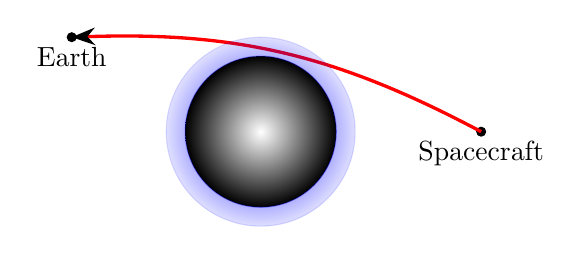
\begin{tikzpicture}[scale=0.8,axis/.style={very thick, ->, >=stealth'},important line/.style={thick},
dashed line/.style={dashed, thin},pile/.style={thick,->, >=stealth', shorten <=2pt,shorten>=2pt},every node/.style={color=black}]
    \coordinate (A) at (3.5,0) {};
    \coordinate (B) at (-3,1.5) {};
    \filldraw[black] (3.5,0) circle (2pt) node[below] {Spacecraft};
    \filldraw[black] (-3,1.5) circle (2pt) node[below] {Earth};
\begin{scope}[>={Stealth[black]},
    every node/.style={fill=white,circle},every edge/.style={draw=red,very thick}]
    \path [->] (A) edge[bend right=15] (B); 
\end{scope}
    \shade [even odd rule,inner color=white,outer color=black!100!gray] (0, 0) circle (1.2cm);
    \filldraw[even odd rule,blue ,path fading=ringo] (0,0) circle (15mm) (0,0) circle (1.2cm);
\end{tikzpicture}
	\caption{Refraction via Atmospheric Occultation}
	\label{fig:usr_planet_occ_1}
\end{wrapfigure}
\gls{rs} is the study of physical objects and phenomena using \gls{radio waves}. Observables include the time, \gls{amplitude}, \gls{frequency}, \gls{phase}, and \gls{polarization} of a received signal. \gls{rs} experiments involve \gls{gravitation} and \gls{propagation}. Cassini served as a point-mass probe within the gravity field of \gls{saturn} and its satellites, precision measurements of the Earth-Cassini distance and \gls{relative velocity} can be used to infer the target body mass and higher order field components. \Gls{propagation} experiments used \glspl{occultation} to study planetary \glspl{ionosphere}, \glspl{neutral atmosphere}, \gls{planetary rings}, \gls{solar plasma}, \gls{cometary comae}, etc. During a planetary \gls{occultation} the spacecraft transmitted a signal that was \glslink{refraction}{refracted} by the target atmosphere and then received on Earth by the \gls{dsn}, as shown in figure \ref{fig:usr_planet_occ_1}. As the spacecraft moved, the signal probed deeper into the atmosphere until it was absorbed by the planet. The figure depicts a one-way \gls{downlink} observation. A \gls{one-way observation} involves a \gls{downlink} spacecraft-to-Earth signal, but no \gls{uplink} Earth-to-spacecraft signal. Stability of the signal depends on the reference \gls{oscillator} on the spacecraft; Cassini used an \gls{uso}. A \gls{two-way observation} involves a \gls{downlink} spacecraft-to-Earth signal and an \gls{uplink} Earth-to-spacecraft signal that is used to control the frequency of the \gls{downlink} signal. This provides better stability due to Earth's atomic clocks. The Earth-spacecraft line-of-sight often contained rings and objects that would distort the signal, making \glslink{one-way observation}{one-way} mode preferable. \Glspl{three-way observation} use two ground stations and the spacecraft. One station transmits a signal to the spacecraft and another receives the signals sent from the spacecraft. This was used when an observation occurred over a period of time that would cause one ground station to be blocked from view of the spacecraft. \glslink{three-way observation}{Three-way} 
\begin{figure}[H]
	\centering
	\includegraphics[page = 15,trim = {1.4cm 1.25in 1.25in 1.08in},clip,width = 0.49\textwidth]{images.pdf}
	\hfill
	\includegraphics[page = 14,trim = {1.4cm 1.25in 1.25in 1.08in},clip,width = 0.49\textwidth]{images.pdf}
	\caption{DSN Elevation maps Rev 280 and Rev 282}
	\label{fig:usr_dsn_elav_map_1}
\end{figure}
\noindent observations were necessary for Cassini due to the $68-84$ minute light travel time from Earth to Saturn. As shown in figure \ref{fig:usr_dsn_elav_map_1}, often times $2$ or $3$ \gls{dsn} stations were needed to complete an observation. Figure \ref{fig:usr_dsn_map_1} shows where the various \gls{dsn} stations are. \Gls{occultation} observations allow for \glslink{temperature-pressure profile}{temperature-pressure} and \glspl{absorption profile} of \glspl{neutral atmosphere}, \glspl{electron density profile} of \glspl{ionosphere}, and \gls{optical depth} and \gls{particle size distribution} profiles of rings to be made. Most measurements were wavelength dependent and some included \gls{polarization} effects. During close encounters the spacecraft antenna was deflected from the Earth direction to point at Saturn's surface or ring plane. These \glslink{one-way observation}{one-way} \gls{bsr} experiments required high \glspl{sampling rate} and yielded dielectric constants of target surfaces and size distributions for ring particles. \gls{gwe} near \glspl{solar opposition} and \gls{sce} were conducted during \glslink{cruise mission}{cruise}. Changes in the Earth-Cassini distance and \gls{relative velocity} could indicate passage of gravitational waves through the space between Earth and Cassini. \glslink{two-way observation}{Two-way} mode was used for high stability. During \glspl{occultation} by the sun \glspl{sce} investigated the \gls{solar corona}. \Glspl{two-way observation} were made for large solar radii, \glspl{one-way observation} for smaller solar radii and higher solar activity. Short radio \glspl{wavelength} are least affected by \gls{solar plasma}, and multiple \gls{wavelength} measurements yield total \gls{electron} content along the \gls{radio path}. 



\subsubsection{Spacecraft \label{subsubsec:usr_spacecraft}}

Cassini was comprised of four primary modules: \gls{hga}, two equipment modules, and a propulsion module. These contained various subsystems, including $12$ science instruments. Three \gls{rtg} were mounted in the equipment modules; an external boom for the magnetometer was attached to the \gls{uem}. \hspace*{\fill}

\subsubsection{\footnotesize Radio Frequency Subsystem \label{subsubsec:usr_rad_freq_subsys}}

\begin{wrapfigure}[13]{r}{0.5\textwidth}
	\centering
	\vspace{-5ex}
	\includegraphics[page = 16,trim = {1.15in 4.1in 1.15in 2.15in},clip,width = 0.5\textwidth]{images.pdf}
	\caption{Map of DSN stations}
	\label{fig:usr_dsn_map_1}
\end{wrapfigure}

The \gls{rfs} provided communications to the \gls{dsn} and a signal source for \gls{rs} measurements. \gls{rs}-only components called the \gls{rfis} are here considered to fall within the \gls{rfs}. It included a pair of redundant \gls{x-band} \glspl{transponder} for reception and transmission, an \gls{s-band} \gls{transmitter}, and a \gls{ka-band}
\gls{transmitter}. The \gls{uso} provided on-board time and \gls{frequency} reference until it failed in $2011$. A \gls{kat}, which received at $34$ GHz and transmitted \glslink{coherent}{coherently} at $32$ GHz, supported \glslink{relativity}{general relativity} observations during the \glslink{cruise mission}{cruise}, but failed during insertion into Saturn's orbit. The \gls{rfs} produced an \gls{x-band} \gls{carrier} \glslink{modulation}{modulated} with data received from the \gls{cds}, amplified the \glslink{modulation}{modulated} carrier, and delivered the signal stream to the antenna subsystem for transmission to Earth. It also received and \glslink{demodulation}{demodulated} \gls{x-band} commands from the ground via the antenna subsystem. Saturn lies between $8.2$ \gls{au} and $10.2$ \gls{au} throughout the year, creating one-way travel times of $68-84$ minutes. Commands from Earth could be received at $1,000$ \gls{bps} by the \gls{hga}, and data could be transmitted to Earth at rates ranging from $14,220-165,900$ \gls{bps}. Data could be recorded on the solid state recorders for $15$ hours while the \gls{hga} was not pointed at Earth, then they were played back for nine hours. About one gigabit of data could be returned each day via a $34$m \gls{dsn} antenna; nearly four times that via a $70$m ground antenna. The two redundant recorders could record and read out nearly $2$ gigabits of data simultaneously. The \gls{cds} handled combined data rates in excess of $430,000$ \gls{bps} from the instruments while carrying on its functions of command and control. Since \gls{rs} observables were generated at the \gls{dsn}, little \gls{tlm} was of interest to \gls{rs}.

\begin{table}[H]
    \centering
    \caption{Cassini RS Bands and Wavelengths}
    \label{tab:usr_band_wav}
    \footnotesize
    \begin{tabular}{|c|c|c|c|}
        \hline
        Band & Wavelength (cm) & Frequence Uplink (MHz)
        & Frequence Downlink (MHz) \\
        \hline
        S  & 13  & N/A   & 2298 \\
        X  & 3.6 & 7175  & 8425 \\
        Ka & 0.9 & 34316 & 32028 \\
        \hline
    \end{tabular}
\end{table}

The antenna subsystem included the $4$m diameter \gls{hga} reflector (Which was also used for sun shading in the early \glslink{cruise mission}{cruise} phase), and two \glspl{lga}. All antennas operated at \gls{x-band}, and only the \gls{hga} operated at \glslink{s-band}{S}, \glslink{ka-band}{Ka}, \glslink{x-band}{X}, and \glslink{ku-band}{Ku} bands. The \gls{x-band} was used for communications, navigations, and \gls{rs}; the \glslink{s-band}{S} and \glslink{ka-band}{Ka} bands were solely for \gls{rs}, and the \gls{ku-band} components were for the Cassini \glslink{radar}{RADAR}. Table \ref{tab:usr_band_wav} lists the various bands and wavelengths which \gls{rs} on Cassini used.

\subsubsection{\footnotesize USO \label{subsubsec:usr_USO}}

\begin{figure}[H]
	\centering
	\vspace{-1ex}
	\begin{subfigure}[b]{0.45\textwidth}
	    \includegraphics[page = 1,trim = {2.2in 5.9in 2.2in 1.1in},clip,width = \textwidth]{images.pdf}
	    \caption{USO Frequency}
	    \label{fig:usr_uso_freq_plot_1}
    \end{subfigure}
    \begin{subfigure}[b]{0.49\textwidth}
        \includegraphics[page = 1,trim = {2.2in 1.6in 2.2in 5.9in},clip,width = \textwidth]{images.pdf}
        \caption{\scriptsize Allen Deviation}
        \label{fig:usr_uso_allen_plot_1}
    \end{subfigure}
        \caption{USO Data}
        \label{fig:usr_uso_freq_allen_dev}
\end{figure}

The \gls{uso} provided the highly stable reference generated on-board the spacecraft until its failure in $2011$. The Cassini oscillator was in the class of high performance thermally-controlled quartz crystal oscillators flown on planetary missions. It was manufactured at the Johns Hopkins University Applied Physics Laboratory. In figure \ref{fig:usr_uso_freq_plot_1} we see the \gls{x-band} output frequency of the \gls{uso} over several years and can see long-term aging behavior (Without accounting for time dilation effects). In figure \ref{fig:usr_uso_allen_plot_1} we see that the \gls{allen deviation} for the \gls{uso} was excellent. In reality this data characterizes the end-to-end performance of the radio systems on both the spacecraft and ground station, although independent calibration of \gls{dsn} stations have shown that these results are dominated primarily by the limit of the \gls{uso} performance. Table \ref{tab:usr_uso_freq_vals} shows the actual values corresponding to the plot in figure \ref{fig:usr_uso_freq_plot_1}. The stability of the \gls{uso} and the small \gls{allen deviation} values allow for \glslink{resolution}{high-resolution} ring profiles to be made, as is discussed in chapter INSERT REFERENCE CHAPTER HERE, section INSERT REFERENCE SECTION HERE. It can be shown, all other factors held constant, that the resolution depends on the \gls{allen deviation} as follows:

\begin{equation}
    R_{res} \propto \frac{\sigma_{t}^2}{e^{-a\sigma_{t}} +a\sigma_{t} - 1}
\end{equation}

Where $\sigma_{t}$ is the \gls{allen deviation} corresponding to $t$-seconds of integration time and $a$ depends on the frequency $f$ and the geometry of the spacecraft.


\begin{table}[H]
    \centering
    \caption{USO Frequency $2006-2011$}
    \label{tab:usr_uso_freq_vals}
    \begin{tabular}{|c c c c c | c c c c c|}
        \hline
        Day & Frequency (Hz) & Year & DOY & & &  Day & Frequency (Hz) & Year & DOY\\
         \hline
         51     & 8427222036.34067  & 2006  & 51  & & & 526  & 8427222041.35297 & 2007 & 161 \\
         76     & 8427222036.52366  & 2006  & 76  & & & 632  & 8427222041.49555 & 2007 & 267 \\
         78     & 8427222036.20419  & 2006  & 78  & & & 712  & 8427222041.63084 & 2007 & 347 \\
         110    & 8427222036.42800  & 2006  & 110 & & & 829  & 8427222042.31336 & 2008 & 99  \\
         123    & 8427222034.34050  & 2006  & 123 & & & 908  & 8427222041.00434 & 2008 & 178 \\
         126    & 8427222043.98074  & 2006  & 126 & & & 937  & 8427222040.45283 & 2008 & 207 \\
         134    & 8427222043.25770  & 2006  & 134 & & & 989  & 8427222040.90144 & 2008 & 259 \\
         141    & 8427222034.29712  & 2006  & 141 & & & 1032 & 8427222041.27468 & 2008 & 302 \\
         159    & 8427222034.62180  & 2006  & 159 & & & 1124 & 8427222042.84108 & 2009 &  28 \\
         178    & 8427222034.66356  & 2006  & 178 & & & 1155 & 8427222043.14919 & 2009 &  59 \\
         196    & 8427222034.83532  & 2006  & 196 & & & 1249 & 8427222043.48567 & 2009 & 153 \\
         214    & 8427222034.92818  & 2006  & 214 & & & 1327 & 8427222044.16133 & 2009 & 232 \\
         232    & 8427222035.09925  & 2006  & 232 & & & 1465 & 8427222045.42919 & 2010 &   4 \\
         242    & 8427222041.00252  & 2006  & 242 & & & 1568 & 8427222046.85504 & 2010 & 107 \\
         248    & 8427222033.76827  & 2006  & 248 & & & 1607 & 8427222047.34145 & 2010 & 146 \\
         260    & 8427222041.02353  & 2006  & 260 & & & 1747 & 8427222049.43250 & 2010 & 286 \\
         320    & 8427222041.37934  & 2006  & 320 & & & 1845 & 8427222050.84059 & 2011 &  19 \\
         353    & 8427222041.70860  & 2006  & 353 & & & 1943 & 8427222052.16839 & 2011 & 117 \\
         356    & 8427222041.74006  & 2006  & 356 & & & 2028 & 8427222053.08372 & 2011 & 202 \\
         393    & 8427222042.06867  & 2007  &  28 & & & 2151 & 8427222055.29388 & 2011 & 325 \\
         436    & 8427222042.17835  & 2007  &  71 & & & 2170 & 8427222055.69421 & 2011 & 345 \\
         \hline
    \end{tabular}
\end{table}

\subsubsection{\footnotesize Attitude and Articulation Control Subsystem \label{subsubsec:usr_att_and_art_cont_subsye}}

The \gls{aacs} maintained the spacecraft's orientation and consisted of redundant sun sensors mounted on the \gls{hga}, redundant stellar reference units mounted on the remote-sensing platform, three mutually perpendicular reaction wheels mounted in the \gls{lem}, and a fourth backup wheel mounted in the \gls{uem}. The \gls{aacs} pointed the selected communication antenna towards Earth and pointed the remote sensing pallet towards the selected target. It also pointed one of the two redundant main propulsion engines in the desired direction during engine burns and performed small trajectory correction maneuvers using the on-board thrusters. The \gls{aacs} used a pointing system known as \gls{inertial vector propagation} that kept track of spacecraft orientation, the direction of the Sun, and distance to the Sun, Earth, Saturn, and other remote sensing targets, and the spacecraft-relative pointing directions of all science instruments. 

\subsubsection{\footnotesize Other Subsystems \label{subsubsec:usr_other_subsys}}

The \gls{pms} was the target subsystem. It consisted of a bi-propellant element for trajectory changes and a \gls{hydrazine} element for attitude control, small maneuvers, and reaction wheel desaturation. The \gls{pps} converted the \gls{rtg} power output to provide a regulated 30-V \gls{dc} power bus and provided the capability to turn various users on or off when commanded. The \gls{tcs} maintained the temperatures of all critical spacecraft components. Even at $9$ \gls{au}, exposing radiator plates to the Sun could severely degrade the data collected by science instruments. The \gls{tcs} could turn electric heaters on or off, open or shut thermal louvers in the \gls{uem}, use small radioisotope heaters, and use thermal blankets and shields.

\subsubsection{\footnotesize Ground Systems \label{subsubsec:usr_ground_sys}}

RS data was acquired by \gls{dsn} stations in Goldstone, California; Canberra, Australia; and Madrid, Spain (See figure \ref{fig:usr_dsn_map_1}), where both $34$m and $70$m antennas were used. Antennas were fixed to lower frequencies when sampled, averaged, and recorded for later analysis. Ground stations were pointed via several different techniques. \Glspl{conical scan} used dynamical ground antenna pointing during which the boresight is offset from the predicted pointing by a small amount. The observed degradation in signal level was used to determine a new pointing direction. This was not used when the signal is expected to undergo significant amplitude changes. \Gls{monopulse} used relative amplitude and phase between $TE_{11}$ and $TE_{12}$ circular \gls{waveguide} mode signals generated in a special \gls{ka-band} feed. \Gls{aberration correction} used a pointing adjustment to account for the real motion of the signal source against the sky background during the one-way light travel time. During \gls{uplink}, the antenna was pointed to the location where the spacecraft will be at the time the signal arrives rather than toward its geometric location at the time of transmission.

\subsubsection{\footnotesize Closed-Loop Tracking Receiver \label{subsubsec:usr_closed_loop_track_rec}}

To track a spacecraft \glslink{carrier}{signal carrier}, the \gls{closed-loop} receiver used a \gls{pll} that measured and recorded the \glslink{carrier}{carrier’s} \gls{phase}. The \glslink{doppler effect}{Doppler} shift is estimated from the phase and converted to relative velocity. \Glspl{ranging code} \gls{modulation} was extracted and correlated with the \gls{uplink} code to determine \gls{absolute range}. The \gls{closed-loop} tracking receiver provided a \glslink{doppler effect}{Doppler} estimate every $0.1$ seconds. \Glspl{ranging sample} were generated at a rate that depends on the code repetition period and user-selected averaging interval.

\subsubsection{\footnotesize Open-Loop Radio Science Receiever \label{subsubsec:usr_open_loop_rad_sci_rec}}

In \gls{open-loop} reception, an independent broad band receiver was used without the \gls{pll} tracking mechanism described above. The \gls{rsr} down-converted the spacecraft signal via a local \gls{oscillator} \gls{heterodyne} process guided by a prediction of the expected \gls{frequency}. It captured and recorded the pre-detection radio signal at a user-selected \gls{sampling rate} via an \gls{analog-to-digital converter}. The digital samples of the propagating electromagnetic wave were stored to disk. Because the received \gls{downlink} signal could be precisely reconstructed, there was great flexibility in signal processing. The \gls{rsr} provided superior \gls{phase stability}, captured the signal during high \gls{amplitude} or \gls{frequency} dynamics, was resilient to \glspl{multi-path effect}, and preserved all information contained in the signal. This method required additional operational procedures, resources, and generation of predictions containing complex planetary atmosphere models. It also involved handling large file sizes and required expertise in digital signal processing. Each \gls{dsn} complex had at least three \glspl{rsr}, each capable of independently capturing the output from a different antenna feed.
\glspl{vsr} were also available for \gls{vlbi} work; their output could be easily converted to the \gls{rsr} format, and they could be used when \gls{cassini} \gls{rs} observations required more support than the \glspl{rsr} alone could provide. The \gls{rssg} remotely operated the \glspl{rsr} and \gls{vsr}s from \gls{jpl}.

\subsubsection{Radio Science Receiver Observables and Analysis}

The spacecraft transmitted a signal at \gls{s-band}, \gls{x-band}, or \gls{ka-band} to a station where the received \gls{rf} was down converted to an \gls{if} of about $300$ MHz and then fed via a \gls{distribution network} into an \gls{rsr}. The signal was then digitized and passed through a digital down converter which selects a $16$ MHz channel through the use of \gls{fir} filters with revolving banks of filter coefficients. The data stream was separated into eight \glslink{decimate}{decimated} data streams that were fed into two sets of filters, one set produced \gls{in-phase} $(I)$ data while the other produced \gls{quadrature-phase} $(Q)$ data. Each of the complex samples contained $8$-bit $I$ and $Q$ components. The output sample size may be $1,2,4,8,$ or $16$. Reduction was accomplished via \gls{truncation}. The samples were unpacked to get $I/Q$ pairs as a function of time. The signal \gls{frequency} could then be computed from the \gls{rsr} by a software \gls{pll} or non-coherently using a \gls{fft}. 

\subsubsection{\footnotesize Sky Frequency}

The \gls{rsr}-level \gls{frequency} can be converted to \gls{downlink} \gls{sky frequency} using tuning information included with \gls{rsr} files. The \gls{rsr} files include two numbers which are valid for the entire file: The radio-frequency-to-intermediate-frequency factor, and the digital down converter local oscillator. For each second of \gls{rsr} data there are three \glspl{frequency-tuning polynomial} $(p_{1},p_{2},p_{3})$. We have:

\begin{align}
sky_{freq}(t) &= F_{R_{f}\rightarrow I_{f}}\cdot 10^{6} + D+dp_{nco}-RSR(t) \label{equ:usr_sky_freq_t}\\
dp_{nco} &= p_1+p_2 \bigg(\frac{n_{msec}}{1000}\bigg)+p_3 \bigg(\frac{n_{msec}}{1000}\bigg)^2 \label{equ:usr_dp_nco}
\end{align}

\noindent Where $F_{R_{f}\rightarrow I_{f}}$ is the radio-frequency-to-intermediate-frequency factor, $D$ is the digital down converter local oscillator, $RSR(t)$ is the signal frequency in the \gls{rsr} output, $p_1,p_2,p_3$ are tuning polynomials found in the \gls{rsr} data files, and $n_{msec}$ is the number of milliseconds within each second's worth of tuning polynomials. 

\subsubsection{\footnotesize Observation Planning \label{subsubsec:usr_obs_planning}}

A \gls{sequence} is an approved list of time-ordered spacecraft activities sent to the spacecraft on a periodic basis. Spacecraft \gls{trajectory} and \gls{attitude} predictions and the quality of reconstruction are crucial to \gls{rs}. During \glslink{cruise mission}{cruise}, the \gls{hga} pointed to Earth and neither \glspl{gwe} nor \glspl{sce} required maneuvers or \gls{attitude} changes. During the \gls{saturn tour}, some \gls{rs} observations had tight timing and pointing requirements. Before these observations the navigation team delivered a special \gls{od} solution and other products to allow the \gls{rs} team to assess the impact of trajectory changes and uncertainties on the observations. The \gls{prime mission} was organized into teams that conduct the \gls{spp} for scientific observations into integrated and conflict-free timelines of the spacecraft's orbit. Orbits are called \glspl{rev}. These teams were the \gls{tost}, \gls{sost}, and the Rings, Saturn, and Cross-Disciplinary \glspl{twt}. Science working groups on surfaces, atmospheres, rings, and \glspl{magnetosphere} also worked to resolve conflicts that cannot be resolved in those teams. This happened for science planning that consisted of production of a \gls{sop} that lead to the generation of a sequence of commands to be sent to the spacecraft. A \gls{svt} was responsible for integrating a conflict-free sequence to the command level. A five-week update process called the aftermarket is applied to the \gls{sop} due to adding science observations, implementation liens, performance changes, or recent scientific discoveries. A final step before \gls{uplink} is called the \gls{ssup}, and starts about $10$ weeks before sequence start date. During the \gls{equinox mission} the process was simplified to just-in-time products: Hand-off packages, checklists, and \gls{dsn} requests that were delivered $2$ weeks prior to \gls{sop} with no aftermarket. The \gls{sop} was a $14$-week process, followed by a $10$-week \gls{ssup}. During the \gls{solstice mission} the process was further simplified to allow integration of the tour with significantly less workforce. Implementation was changed to one process called \gls{sip} which was divided into five ports. The first port began with the integration hand-off products. The next two began with the end products from the previous ports. The remaining were completed with a safe flyable sequence. The sequence development lasted $22$ weeks (Compared to $24$ for Equinox). Sequence execution was $10$ weeks (Compared to $5$ for equinox). 
\par
The \gls{rs} team particapted in planning by proposing observations and following up the process throughout its various stages. The configuration of which of the three possible frequency bands would be used is called an \gls{opmode}. Due
to the normal spacecraft power reduction, other instruments had to be powered off or go into sleep mode to save the power needed to allow \gls{rs} to use certain \glspl{opmode}. Some \gls{rs} observations, such as atmospheric \glspl{occultation}
and Titan \gls{bsr} observations, had tight timing and pointing requirements that could only be met if the designs were updated a few days before the observation execution. Shortly before these observations, the Navigation team delivered a special \gls{od} solution and other products to allow the \gls{rs} team to assess the impact of trajectory
changes and uncertainty on the observations. If needed, timing and/or pointing changes
were made and \glslink{uplink}{uplinked} to the spacecraft.

\subsubsection{Data Archives}

Files with science observables include \gls{closed-loop} \glslink{doppler effect}{Doppler} as well as \gls{open-loop} \gls{rsr} recordings. Each \gls{closed-loop} receiver generated a \gls{tnf}. These typically contain \glslink{doppler effect}{Doppler} \gls{phase} measurements, \gls{ddor} values, and ground system status information. An \gls{odf} is an abstracted version of the \gls{tnf}. Its primary content is line-of-sight \glslink{doppler effect}{Doppler} and range. An \gls{odf} usually represents the output from the \gls{closed-loop} tracking system following a single spacecraft over \gls{dsn} tracking sessions. 

\subsubsection{\footnotesize RSR \label{subsubsec:usr_RSR}}
\Gls{open-loop} data were captured in the \gls{rsr} \gls{sfdu}. \gls{rsr} output samples at a single rate and are stored in records with housekeeping data from the \gls{rsr}. Measured observables require proper calibrations to correct for deterministic error sources. Sample
resolution and rate can vary from $16$ \glspl{bit} at $1$ \gls{khz} to $1$ \gls{bit} at $16$ \gls{mhz}. Each \gls{rsr} could
capture data from a different band and \gls{polarization} pair.

\subsubsection{\footnotesize Other}
Calibration files are provided by the \gls{dsn} for ground-based elements of the \gls{rs} instrumentation and by the flight project for the spacecraft elements. Data in the \gls{dsn} \gls{eop} file describe the motion of the Earth in inertial space in terms of the orientation of its rotation axis and the angle through which the Earth has rotated on its spin axis since some reference epoch. The EOP file is used to calculate the Doppler contribution to a measurement from Earth's rotation. \gls{tro} and \gls{ion} files contain estimates of the radio delay in the Earth's troposphere and ionosphere. The fixed \gls{wvr} measure water emission in the atmosphere. At selected \gls{dsn} stations an \gls{awvr} measures emissions
at $20.7$ and $31.4$ \gls{ghz} along the line-of-sight to the spacecraft being tracked. The \gls{wvr} is part of \gls{dsn} operations; the \gls{awvr} is remotely operated for the \gls{dsn} by the \gls{rssg} from Pasadena. It is an element of a bigger \gls{amc} system. The \gls{dsn} generated a real-time stream of status and performance data from its own
systems ‘monitor’ data; the data may be used for anomaly resolution, performance
validation, and calibration of other data. Some Cassini \gls{rss} data sets include edited versions of this stream. Parameters may include \gls{azimuth} and \gls{elevation} angles of the antenna, \gls{monopulse} correction values, \gls{carrier} \gls{frequency}, wind speed and direction, lock status of the \gls{closed-loop} \gls{pll}, receiver system noise temperature, and \gls{carrier} \gls{snr}. The data are stored in ASCII tables with labels, which describe both the format and content. 

\subsubsection{\footnotesize SPK and CKF}

The Navigation Team provides a reconstructed spacecraft trajectory \gls{spk} after spacecraft maneuvers. The \glspl{ephemeris} of Earth, Saturn, and its moons are included and allow \glslink{doppler effect}{Doppler} calibration of the \gls{rs} data. The team also provides \gls{ckf} files of reconstructed spacecraft orientation. 
%
\subsection{Radio Science Investigations}
%
\subsubsection{Gravity}
%
\noindent Precise distance and velocity measurements of spacecraft under the influence of a target body's \gls{gravitational field} helps measure characteristics of the body. \gls{rs} in celestial mechanics began with \glslink{mariner}{Mariner $2$} and \gls{ranger} in $1962$ to Venus and the Moon, respectively. \gls{ranger} was able to make an estimate of the offset of the lunar \gls{center of gravity} and lunar \gls{center of figure}. Earth and Moon masses were also measured. \glslink{mariner}{Mariner $4,5$, and $9$} made first estimates of low order gravitational harmonics for Venus and Mars. \glslink{doppler effect}{Doppler} measurements from the \gls{lunar orbiter} and \gls{apollo} missions led to the discovery of large positive gravity anomalies, called \glspl{mascon}, on the moon. The mean density of a planet is determined from its bulk volume and mass. Volume is derived from a shape model based on images, topographic \gls{altimetry}, and radio \glspl{occultation}. Mass is obtained via measurements of gravity. Information about the internal structure of the body, when combined with an optical or radar map of surface features,
can constrain modelling the differentiation of interior layers and the chemical composition and physical state of the interior. Cassini was used to study Saturn and its gravity field. Measurements of \gls{titan}, \gls{enceladus}, \gls{rhea}, and \gls{dione} were also made. \glslink{titan}{Titan's} mass and \gls{gravitational harmonics} have been measured to degree $3$. \glslink{titan}{Titan's} \gls{quadrupole} field is consistent with a \glslink{hydrostatic}{hydrostatically} relaxed body, shaped by tidal and rotational forces. The inferred \gls{moment of inertia} is about $0.34$, implying incomplete differentiation either in the sense of imperfect separation of rock from ice, or a core in which a large amount of water remains chemically bound in silicates. Non-hydrostatic \gls{geoid}
height variations of up to $19$ meters are small compared to the observed topographic anomalies of hundreds of meters, suggesting a high degree of compensation appropriate to a body that has warm ice at depth.

\subsubsection{\footnotesize Field Representation}

The \gls{gravitational field} is represented by an $n^{th}$ degree and order \gls{spherical harmonic} series expansion. $GM$ scales the harmonics of the field ($G = 6.67 \times 10^{-11} N\frac{m^2}{kg^2}$, $M$ is mass). Additional lower degree terms describe the dynamic flattening
and the orientation of the \gls{principal rotation axes} while placing constraints on the deep interior structure. Higher degree terms describe smaller and shallower local gravity features near the surface, including mountains and craters. This representation follows from the solution to \gls{laplace's equation}:

\begin{equation}
U = \frac{GM}{r}\bigg(1+ \sum_{n=2}^{\infty} \sum_{m=0}^{n} \bigg(\frac{R_{e}}{r}\bigg)^n\overline{P}_{nm}\big(\sin(\phi_{lat})\big)\big[\overline{C}_{nm}\cos(n\lambda)+\overline{S}_{nm}\sin(m\lambda)\big]\bigg)
\end{equation}

\noindent Where $R_{e}$ is the reference radius of the sphere, $\phi_{lat}$ is the latitude, $\lambda$ is the longitude, $\overline{C}_{nm}$ and $\overline{S}_{nm}$ are the normalized coefficients satisfying boundary conditions, and $\overline{P}_{nm}$ are the normalized associated Legendre functions. The un-normalized coefficients are:

\begin{equation}
\begin{bmatrix}
C_{nm} \\
S_{nm}
\end{bmatrix} =
\bigg(\frac{(n-m)!(2n+1)(2-\delta_{0m})}{(n+m)!}\bigg)^{1/2}
\begin{bmatrix}
\overline{C}_{nm} \\
\overline{S}_{nm}
\end{bmatrix}
\end{equation}
\noindent where $\delta_{ij}$ is the \gls{kronecker delta}, and $n$ and $m$ describe surface resolution.
\subsubsection{\footnotesize Data Processing}
\begin{wrapfigure}[7]{l}{0.45\textwidth}
	\centering
	\vspace{-2.5ex}
	\resizebox {0.45\textwidth} {1in} {
    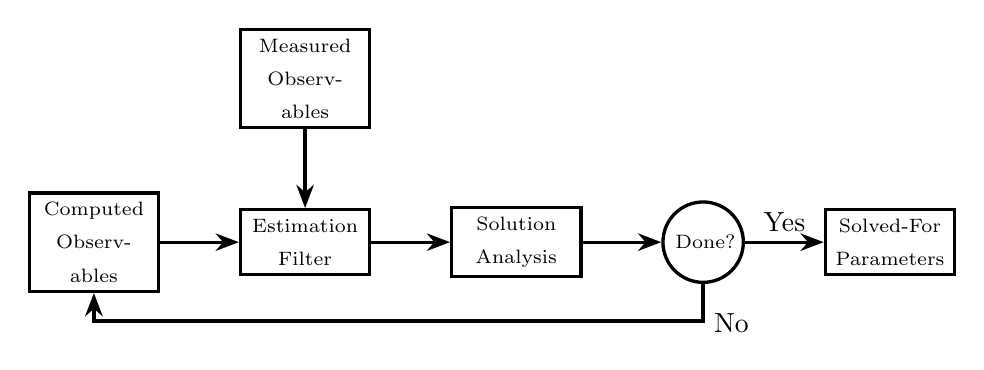
\begin{tikzpicture}
    %Nodes
    \begin{scope}[
    roundnode/.style={circle, draw=black, very thick,text width=2em,text centered}, squarednode/.style={rectangle,text width=4em,text centered, draw=black, very thick},
    every edge/.style={draw=black,very thick}]
    \node[squarednode]      (1)     {\scriptsize{Computed Observables}};
    \node[squarednode]        (2)       [right=of 1] {\scriptsize{Estimation Filter}};
    \node[squarednode]      (3)       [above=of 2] {\scriptsize{Measured Observables}};
    \node[squarednode] (4) [right=of 2] {\scriptsize{Solution Analysis}};
    \node[roundnode]        (5)       [right=of 4] {\scriptsize{Done?}};
    \node[squarednode] (6) [right=of 5] {\scriptsize{Solved-For Parameters}};
    \end{scope}
 
    %Lines
    \begin{scope}[>={Stealth[black]},
              every edge/.style={draw=black,very thick}]
        \path[->] (1) edge (2);
        \path[->] (3) edge (2);
        \path[->] (2) edge (4);
        \path[->] (4) edge (5);
        \path[->] (5) edge node[above] {Yes} (6);
    \end{scope}
    
    \draw[>={Stealth[black]},very thick,->] (5) -- node[below  right] {No} ++(0,-1cm) -|  (1);
    
    \end{tikzpicture}
    }
	\caption{Flow Diagram for Gravity Solution}
	\label{fig:usr_flow_diagram_gravity}
\end{wrapfigure}

The procedures for deriving \gls{gravitational field} models are closely linked to the \gls{od} problem for interplanetary spacecraft. This is an iterative process based on the comparison between measured observables and the corresponding values in the \gls{moyer model}. For Cassini, the parameters that are estimated are the $GM$ value, the coefficients for the \gls{spherical harmonic} expansion, the \gls{love numbers} that define the field response to external tidal forces, and the target's rotational parameter's. The \gls{od} process can be divided into four steps:

\begin{enumerate}[itemsep=0pt]
\begin{multicols}{2}
\item[1.] Pre-process measured observables.
\item[3.] Apply estimation filter.
\item[2.] Calculate computed observables.
\item[4.] Solution analysis.
\end{multicols}
\end{enumerate}

\noindent The solution is intrinsically non-linear. Figure \ref{fig:usr_flow_diagram_gravity} depicts the iterative nature of the method. The primary observables are:

\begin{enumerate}[itemsep=0pt]
\item \Gls{range}: Measured round-trip light time, or distance, in range units.
\item \glslink{doppler effect}{Doppler}: Measured frequency shift of the carrier of the received signal due to relative transmitter-receiver motion.
\item \gls{ddor}: The measured angular position of the spacecraft in the plane of the sky along a baseline formed by two ground stations.
\end{enumerate}

\noindent Before \gls{od} analysis we may apply calibrations to observables to correct for \glspl{group delay} due to ground and spacecraft electronics and group and \glspl{phase delay} due to the \gls{troposphere}, \gls{ionosphere}, and \gls{interplanetary plasma}. We can also compute received \glspl{sky frequency} from \gls{open-loop} recordings, compute synthetic non-dispersive observables using a multi-frequency link, and delete \glspl{outlier}.

\subsubsection{\footnotesize Calculation of Observables}

During the calculation step, observables are computed using mathematical models of all non-negligible physical effects. These models depend on three types of parameters:

\begin{enumerate}[itemsep=0pt]
\item \glslink{solve-for parameters}{Solve-For Parameters}: A set of model parameters whose current estimate can be improved through the \gls{od} process and for which the estimation filter computes a differential correction of their central values along with their uncertainties, in the form of a \gls{covariance matrix}.
\item \glslink{consider parameters}{Consider Parameters}: Not-exact parameters that affect the data and whose current estimate cannot be improved through the \gls{od} process.
\item \glslink{exact parameters}{Exact Parameters}: Parameters with uncertainties that do not affect the estimation because they are negligible with respect to their influence on observables.
\end{enumerate}

\subsubsection{\footnotesize Planetary/Satellite Ephemeris Update}

It may be necessary to update planetary and/or satellite \glspl{ephemeris}. For example, during observations of a satellite the Cassini trajectory is affected in a non-negligible way by the \glspl{gravitational field} of both Saturn and the satellite. The measured observables are sensitive to the relative positions and velocities of the spacecraft, the satellite, and the planet. Errors in the satellite \gls{ephemeris} may alias into estimation errors on the spacecraft state and/or the satellite gravity coefficients. Satellite \glspl{ephemeris} must be updated as a part of the \gls{od} process. For the first iteration, the most recent \gls{ephemeris} is used. In subsequent iterations, the solution obtained from the previous iteration is used. Updated \glspl{ephemeris} are generated by integrating the full relativistic \gls{equations of motion} of the planets and the satellites from their updated initial states. To compute the partials and update the \glspl{ephemeris}, the \glspl{variational equation} are integrated.

\subsubsection{\footnotesize Integration of Equations of Motions and Variational Equations}

Calculations of observables and their partial derivatives require reconstructing the spacecraft trajectory by integrating the \gls{equations of motion} with respect to a non-rotating reference frame, which includes the coordinate system origin or \gls{coi}, from an initial state. All non-negligible forces must be modeled. These include:

\begin{enumerate}[itemsep=0pt]
\item Newtonian gravitational acceleration due to the Sun and planets/satellites.
\item Relativistic perturbing gravitational acceleration due to the Sun/planets/satellites.
\item Acceleration from geodesic precession.
\item Acceleration from Lense-Thiring precession.
\item Newtonian acceleration due to the gravitational spherical harmonics of solar bodies.
\item Relativistic acceleration of the gravitational spherical harmonics.
\item Accelerations caused by tidal effects on the physical central body.
\item Acceleration by time-varying gravity effects such as atmospheric or ice movement.
\item Gravitational acceleration due to planetary rings.
\item Gravitational acceleration due to mascons.
\item Solar and Planetary radiation pressure.
\item Atmospheric drag.
\item Gas leakage: Acceleration due to spacecraft control jet leakage.
\item Maneuvers.
\item Thermal inbalance: Acceleration due to non-uniform spacecraft surface heating.
\end{enumerate}

\subsubsection{\footnotesize Time Transformations}

\noindent Observables are time-stamped by the station clock in \gls{utc}. For the light-time solution to be computed time must be expressed in \gls{tcb}. Time can also be expressed as linear transformations of \gls{tcb}, such as \gls{et} or \gls{tdb}.

\subsubsection{\footnotesize Ground Station State Computation}

The location of a ground station is conventionally defined as the position of a reference point whose coordinates are given as inputs in a terrestrial reference frame. The location of a ground station must be corrected to account for various effects:

\begin{enumerate}[itemsep=0pt]
\item \glslink{solid earth tides}{Solid Earth Tides}: Solar and Lunar tides.
\item \glslink{ocean loadings}{Ocean Loadings}: Displacements from ocean tides.
\item \glslink{pole tides}{Pole tides}: Modifications from polar motion.
\item \glslink{plate motion}{Plate motion}: Motion from tectonic plates.
\item Offset between the center of mass and center of figure of Earth.
\item Offset between phase and reference point center.
\end{enumerate}

\noindent To solve for light-time it is necessary to convert the station location from the terrestrial reference frame to the celestial reference frame. This transformation consists of a series of rotations: Polar motion, Earth rotation, \gls{nutation}, and \gls{precession}. These rotations are characterized by a set of parameters that depend on the particular selected models. \gls{jpl} and \gls{eop} define these rotations according to the \gls{iau} $1980$ theory of \gls{nutation} and the \gls{iau} $1976$ \gls{precession} model. After these rotations, the geocentric state of the tracking
station is expressed in the geocentric space-time frame of reference, and it must be referred to the solar-system barycentric space-time frame of reference through proper
\glspl{lorentz transformation}.

\subsubsection{\footnotesize Light-Time Computation}

The final part is obtaining the light-time solution in the solar-system barycentric frame. Solving this problem involves:

\begin{enumerate}[itemsep=0pt]
    \item The receiving station at reception time $t_1$.
    \item The spacecraft at the reflection time for \glslink{two-way observation}{two-way} and \glslink{three-way observation}{three-way} observables or transmission time for \glslink{one-way observation}{one-way} observables $t_2$.
    \item The transmitting station at the transmission for \glslink{two-way observation}{two-way}/\glslink{three-way observation}{three-way} observables $t_1$.
\end{enumerate}

In the \gls{od} process, the reception time of an observable is known, so it is necessary to solve the light-time to find the transmission and the reflection times. The light-time
problem is based upon the known speed of light and travel time from the transmitter to the receiver, which has two components:

\begin{enumerate}[itemsep=0pt]
    \item Newtonian light time (Time for light to travel along a straight-line path at $c$).
    \item Relativistic light-time delay (The \gls{shapiro effect})
\end{enumerate}

\subsubsection{\footnotesize Estimation Filter}

The estimation filter computes parameter values that minimize the following in a \glspl{least squares} sense:
\begin{enumerate}[itemsep=0pt]
\item Residual difference between the measured and computed observables.
\item Differences between the solve-for parameters and their $a\ priori$ values.
\end{enumerate}

The estimation filter produces two outputs:

\begin{enumerate}[itemsep=0pt]
    \item A differential correction to \textit{a priori} values of the \gls{solve-for parameters}.
    \item The \gls{covariance matrix} of the \gls{solve-for parameters} that represents the solution uncertainty. The matrix is updated based on the influences of measurement noise and \glslink{consider parameters}{consider parameter} uncertainties on the \gls{solve-for parameters}
\end{enumerate}

\subsubsection{\footnotesize Solution Analysis}

\noindent The solution obtained from the estimation filter is verified and tested using these criteria:
\begin{enumerate}[itemsep=0pt]
\item Convergence: The \gls{od} Process reaches convergence if two or more successive iteration steps produce statistically equivalent solutions.
\item Residual Analysis: The obtained solution is used to compute \glspl{residual}. If the \gls{od} process was performed correctly, the solution \glspl{residual} represent only measurement noise and hence must satisfy the following:
\begin{enumerate}[itemsep=0pt]
\item Zero mean: \Gls{residual} means must be much less than their standard deviations.
\item Spectrum of \glspl{residual} is compatible with the expected noise characteristics.
\item The \gls{residual} standard deviations should be compatible with the \gls{residual} \break weights used in the estimation filter.
\end{enumerate}
\item Solution \gls{covariance matrix} analysis:
\begin{enumerate}[itemsep=0pt]
\item Comparison between \textit{a priori} and computed formal uncertainties.
\item Cross-correlation between \gls{solve-for parameters}.
\end{enumerate}
\item Comparison between \textit{a priori} values and the new estimates.
\item Solution stability.
\end{enumerate}

\begin{example}[Rhea] Consider Cassini's fly-by of Rhea on November 26, 2005. Data reduction was based on least squares filtering of the Doppler residuals that were generated by comparing measure sky frequencies with calculated values. The calculations depended on the spacecraft state vector at the starting epoch and its dynamic environment, including:
\begin{enumerate}[itemsep=0pt]
\item Motion of solar system bodies.
\item Ground station locations and Earth rotation dynamics.
\item Gravitational accelerations on spacecraft.
\item Non-gravitational accelerations on spacecraft.
\item Relativistic effects and signal propagation model.
\end{enumerate}
\end{example}

\subsubsection{\footnotesize Rhea: Solve-For Parameters}

\noindent \Gls{solve-for parameters} always include the spacecraft epoch state-vector $x$ hours before closest approach. It was necessary to solve for Rhea's initial state vector. The minimum set of gravity coefficients contained \gls{monopole} and \gls{quadrupole} fields $(GM, J_2, C_{21}, S_{21}, C_{22}, S_{22})$. Degree $3$ and higher requires additional fly-bys.

\subsubsection{\footnotesize Rhea: Consider Parameters}

The \textit{a priori} uncertainties ($\sim 10^{-9}\textrm{m/s}^2$) of the \gls{rtg}-induced acceleration and the thermo-optical properties of the spacecraft cannot be inferred by fly-by data, but the can be included as \gls{consider parameters}. 

\subsubsection{\footnotesize Rhea: Exact Parameters}

A detailed model of the Earth's rotation was included to provide the correct inertial state of the ground stations. \gls{eop} data are usually obtained from the \gls{iers}. Perturbations due to the gravity of the Sun, Jupiter, Saturn, and Saturnian satellites were included.

\subsubsection{\footnotesize Rhea: \textit{a priori} Uncertainties} 
The \gls{covariance matrix} is a full \gls{symmetric matrix}. It is difficult to compute \textit{a priori} correlations if previous data is not available. In this case, the covariance matrix was initialized to be \glslink{diagonal matrix}{diagonal}.

\subsubsection{\footnotesize Rhea: Pre-processing of Radiometric Measurements}

\glslink{doppler effect}{Doppler} tracking of the spacecraft during the fly-by provided the time-dependent \gls{sky frequency}, which is the frequency of the signal sent back by the spacecraft as it is received on Earth by the ground station. This frequency contained, among many other things, the \glslink{doppler effect}{Doppler shift} caused by Rhea’s gravitational influence on Cassini’s fly-by trajectory.

\subsubsection{\footnotesize Rhea: Data Selection}

Cassini tracking data could be acquired in either \glslink{two-way observation}{two-way} or \glslink{three-way observation}{three-way} mode. \Gls{carrier} frequency options included \gls{x-band} \gls{downlink} \gls{coherent} with \gls{x-band} \gls{uplink} $(X/X)$, or \gls{ka-band} \gls{downlink} \gls{coherent} with \gls{x-band} uplink $(X/K_{a})$. \glslink{two-way observation}{two-way} is usually preferred over \glslink{three-way observation}{three-way}, since the same \gls{frequency} standard is used throughout the signal round trip time. $X/K_{a}$ is usually preferred over $X/X$ due to the former’s higher immunity to \gls{plasma} noise on the \gls{ka-band} \gls{downlink}. In the $2005$ \gls{rhea} flyby, a combination of these data types was available: \glslink{two-way observation}{two-way} in $X/X$ and $X/K_{a}$, and \glslink{three-way observation}{three-way} in $X/K_{a}$.

\subsubsection{\footnotesize Rhea: Data Compression}

Each Doppler measurement is characterized by its count time. \Gls{compression}, or averaging data over a larger count time, reduces the number of data points and associated noise. When only low-degree harmonics were sought, count times as long as $60$ seconds were used.

\subsubsection{\footnotesize Rhea: Group and Phase Delay Calibration}

Corrections were applied to account for phase and time delays due to Earth's \gls{troposphere} and \gls{ionosphere}. Data from the \gls{awvr} was used to compensate for tropospheric effects.

\subsubsection{\footnotesize Rhea: Estimation Filter}

Frequency residuals for a given iteration were obtained by comparing the observed \glspl{sky frequency} with predictions based on the numerically computed trajectory integrated using the current dynamical model. The residuals were the main input to the data-filtering algorithm; the goal was to minimize the sum of squared residuals. The pre-fit residuals were numerically computed starting from some \textit{a priori} knowledge of the spacecraft state vector and dynamical model parameters. A plot of pre-fit residuals vs. time may show the effects of errors due to observation noise, unoptimized values of parameters of the mathematical model, and inadequacies of the underlying models of the actual phenomena.
Figure \ref{fig:usr_pre_fit_rhea_grav_exp} shows the pre-fit frequency residuals computed from the nominal dynamical model. The residuals contain signatures due to observation noise, errors in the mathematical model and errors in the values of model parameters. Errors in the dynamical model are particularly evident near closest approach. Figure \ref{fig:usr_post_fit_rhea_grav_exp} shows the post-fit frequency residuals. Fitted parameters have been updated with the least squares solution, and the model trajectory fits the \glslink{doppler effect}{Doppler} data extremely well.

\begin{figure}[H]
	\centering
	\begin{subfigure}[b]{0.48\textwidth}
	    \includegraphics[page = 2,trim = {1.6in 4.9in 1.6in 3.2in},clip,width = \textwidth]{images.pdf}
	    \caption{\scriptsize Pre-Fit Residuals}
	    \label{fig:usr_pre_fit_rhea_grav_exp}
    \end{subfigure}
    \begin{subfigure}[b]{0.5\textwidth}
        \includegraphics[page = 2,trim = {1.6in 1.7in 1.6in 6.7in},clip,width = \textwidth]{images.pdf}
        \caption{\scriptsize Post-Fit Residuals}
        \label{fig:usr_post_fit_rhea_grav_exp}
    \end{subfigure}
        \caption{Residual Fits of a Rhea Gravity Experiment}
        \label{fig:usr_rhea_grav_exp}
\end{figure}

\subsubsection{\footnotesize Rhea: Solution Analysis and Results}

The Cassini spacecraft encountered Rhea on November $26$, $2005$, and analysis of the Doppler data acquired at and around closest approach yields the mass of Rhea and the \gls{quadrupole} moments of its \gls{gravitational field} with unprecedented accuracy: $GM=153.9395\pm 0.0018 km^{3}s^{-2}$, which corresponds to a density of $1232.8\pm 5.4
kg m^{-3}$. The results for $J_{2}$ and $C_{22}$ are $(7.947\pm 0.892)\times 10^{-4}$ and $(2.3526\pm 0.0476)\times 10^{-4}$, respectively. These values are consistent with \gls{hydrostatic} equilibrium. From the value of $C_{22}$, the non-dimensional moment of inertia $\frac{C}{MR^{2}} = 0.3721 \pm 0.0036$. Models of \glslink{rhea}{Rhea's} interior based on the gravity data favored an almost undifferentiated satellite. A discontinuity between a core and a mantle is possible but not required by the data. Models with a constant silicate mass fraction throughout the body cannot account for the determined \gls{quadrupole} coefficients. The data exclude fully differentiated models in which the core would be composed of unhydrated silicates and the mantle would be
composed of pure ice. If the mantle contains $10\%$ in mass of silicates, the core extends to
630 km in radius and has a silicate mass fraction of $40\%$. A continuous model in which
the silicates are more concentrated toward the center of the body than in the outer layers is allowed by the gravity data but excluded by thermal evolution considerations. The one model that fits the gravity data and is self-consistent when energy transport and ice melting are qualitatively considered is an almost undifferentiated \gls{rhea}, in which a very large uniform core is surrounded by a relatively thin ice shell containing no rock at all.
\subsubsection{Atmosphere}
Radio occulting techniques can be used to investigate planetary \glspl{atmosphere} and \glspl{ionosphere}. The radio link is perturbed in \gls{phase} and \gls{amplitude} by intervening \gls{plasma} and/or neutral gas. The measured perturbation on the ground can be converted into an atmospheric refractivity profile. From this, \glslink{electron density profile}{electron distribution} in the \gls{ionosphere} or \gls{temperature-pressure profile} in the \gls{neutral atmosphere} can be derived. \Gls{occultation} techniques were first demonstrated in $1965$ when \glslink{mariner}{Mariner IV} flew by Mars and determined the salient features of the Martian \gls{atmosphere}. The observation's showed the surface pressure is less than one percent of Earth's, which is an order of magnitude less than had been previously believed. During \glslink{mariner}{Mariner V's} flyby of Venus, a radio \gls{occultation} experiment gave a \gls{temperature-pressure profile} in the \gls{neutral atmosphere} and the \gls{electron density profile} in the ionosphere. 
\subsubsection{\footnotesize Neutral Atmosphere}
The radio \gls{occultation} technique relies on successful inversion of the observed changes in the \gls{frequency} and \gls{amplitude} of the radio signals during the atmospheric \gls{occultation} period to produce vertical profiles of the \gls{index of refraction} and \gls{absorption coefficient}. This technique is established for the case of radial symmetry. In a \glslink{one-way observation}{one-way} \gls{downlink} experiment, the ray between a spacecraft and Earth is \glslink{refraction}{refracted} by the planet's \gls{atmosphere}, \makebox[\linewidth][s]{as shown in figure \ref{fig:usr_atmo_occ_geo}. $\alpha$ is the \gls{bending angle}, $p=\norm{\mathbf{p}_{out}}=\norm{\mathbf{p}_{in}}$ is the ray asymptotic}
\begin{wrapfigure}[12]{l}{0.5\textwidth}
	\centering
	\vspace{-2ex}
	\resizebox{0.5\textwidth}{!}{
    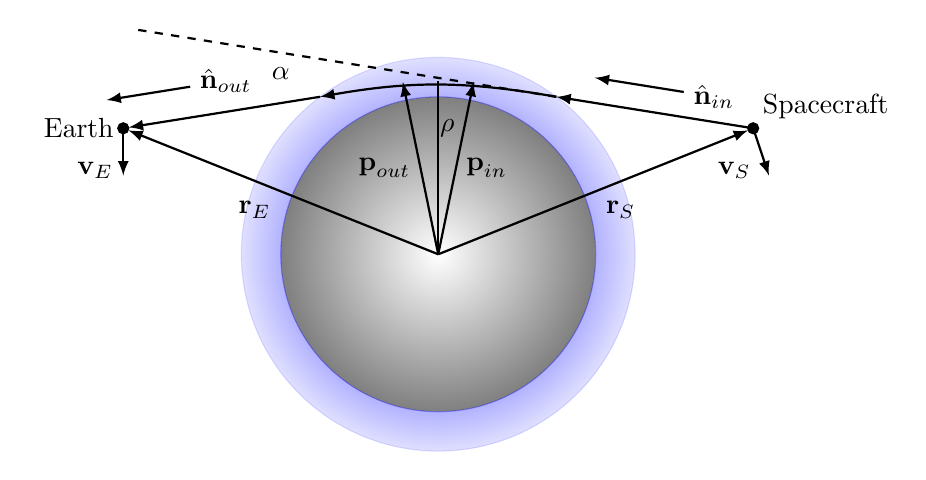
\begin{tikzpicture}[axis/.style={very thick, ->, >=stealth'},important line/.style={thick},
    dashed line/.style={dashed, thin},pile/.style={thick,->, >=stealth', shorten <=2pt,shorten>=2pt},every node/.style={color=black}]
    \coordinate (S)  at (4,1.6);
    \coordinate (E)  at (-4,1.6);
    \coordinate (O)  at (0,0);
    \coordinate (p1) at (-1.5,2);
    \coordinate (p2) at (1.5,2);
    \coordinate (P) at (0,2.2);
    \shade [even odd rule,inner color=white, outer color=gray] (0, 0) circle (2cm);
    \filldraw[even odd rule,blue ,path fading=ringo] (0,0) circle (25mm) (0,0) circle (2cm);
    \filldraw[black] (E) circle (2pt) node[left] {Earth};
    \filldraw[black] (S) circle (2pt) node[above right] {Spacecraft};
\begin{scope}[>={latex[black]},every edge/.style={draw=black,thick}]
    \path [->] (S) edge (p2);
    \path [->] (p2) edge[bend right=10] (p1);
    \path [->,shorten >=2pt,shorten <=0cm,->] (p1) edge (E);
    \path [->] (O) edge node[right] {$\textbf{p}_{in}$} (0.45,2.18874);
    \path [->] (O) edge node[left] {$\textbf{p}_{out}$} (-0.45,2.18874);
    \path [->,shorten >=2pt,shorten <=0cm,->] (O) edge node[below left] {$\mathbf{r}_{E}$} (E);
    \path [->,shorten >=2pt,shorten <=0cm,->] (O) edge node[below right] {$\mathbf{r}_{S}$} (S);
    \path [->] (S) edge node[below left] {$\mathbf{v}_{S}$} (4.2,1);
    \path [->] (E) edge node[below left] {$\mathbf{v}_{E}$} (-4,1);
    \path (O) edge (P);
\end{scope}
\node (nin) at (3.5,2) {$\hat{\mathbf{n}}_{in}$};
\node (nout) at (-2.7,2.2) {$\hat{\mathbf{n}}_{out}$};
\draw[>={latex[black]},thick,shorten >=1cm,shorten <=0cm,->] (nin) -- +($(p2)-(S)$);
\draw[>={latex[black]},thick,shorten >=1cm,shorten <=0cm,->] (nout) -- +($(E)-(p1)$);
\draw[thick,dashed] (p2) -- ($(S)!8cm!(p2)$);
\node at (-2,2.3) {$\alpha$};
\node at (-0.1,1.6) [right] {$\rho$};
\end{tikzpicture}}
	\caption{Geometry of an Occultation of Titan}
	\label{fig:usr_atmo_occ_geo}
\end{wrapfigure}

\noindent distance, and $\rho$ represents the center of refraction. The position of the spacecraft when the photon was emitted is $\mathbf{r}_{S}$, and the position of the antenna on Earth when the photon was received is $\mathbf{r}_{E}$. The geometry is iteratively computed from the \glspl{ephemeris} of the spacecraft, planet center, and Earth center relative to the Sun. Spacecraft position and velocity, measurements of \glslink{doppler effect}{Doppler shift}, and the assumption of spherical symmetry determine $\alpha$ as a function of $p$. This is used to compute a refractivity profile or the \gls{atmosphere} and then a \gls{temperature-pressure profile}.

\subsubsection{\footnotesize Analysis}

Occultations occurring after the failure of the \gls{uso} were done in \glslink{two-way observation}{two-way} mode. Both the \gls{uplink} and \gls{downlink} rays pass through the \gls{atmosphere} under study making analysis complicated. Only \glspl{occultation} prior to $2011$ are discuessed. The \gls{rs} team uses two different techniques to invert \glslink{one-way observation}{one-way} data. Ray tracing uses geometrical optics to trace rays from the spacecraft to the receiving antenna, simultaneously solving for the structure of the \gls{atmosphere} as each successive ray is traced. When the target \gls{atmosphere} is spherically symmetric, a faster and simpler \gls{abel transform} directly connects the \gls{bending angle} between the ray leaving the spacecraft and the ray arriving at the ground station with the index of refraction of the gas. The \gls{abel transform} is used for \gls{titan}, and ray tracing is used for Saturn. Saturn is significantly oblate and its atmosphere supports planetary scale zonal winds, which further complicate the atmospheric structure. The Cassini team allows a restricted (Barotropic assumptions) differential wind field.

\subsubsection{\footnotesize Converting Raw RSR Data to Usable Forms}

Prior to the failure of the \gls{uso}, the spacecraft could emit simultaneously at three \gls{uso}-driven frequencies at \gls{s-band}, \gls{x-band}, and \gls{ka-band}. These are considered constant in the spacecraft's rest frame. When any of these signals are received at a ground station, they're immediately mixed with a local \gls{dsn} fixed-frequency local oscillator signal that down-converts it from \gls{ghz} range to the $300$ \gls{mhz} range and delivers it to an \gls{rsr}. The output is digitized and a programmable local oscillator down-converts again to the $0-100$ \gls{khz} range. The tunable local oscillator is generated from an \gls{rsr} \gls{frequency} prediction file, which is pre-computed by the \gls{rssg} using a model of the \gls{atmosphere} and a predicted \gls{ephemeris} of the spacecraft. The \gls{open-loop} recordings typically have sampling rates of $1-100$ \gls{khz}. The resulting time series of antenna voltages is contained in the \gls{rsr} output file, along with the local oscillator frequency in the form of piece-wise polynomials, see Eqn.~\ref{equ:usr_sky_freq_t}. For an \gls{occultation} in \glslink{two-way observation}{two-way} mode, a model of the \gls{atmosphere} and a predicted \gls{ephemeris} are used to compute the \gls{uplink} \gls{frequency} to be sent from a ground station. The paths of the \gls{uplink} and \gls{downlink} signals through the \gls{atmosphere} are similar, but not identical. The \gls{atmosphere} model is used to compute the \gls{frequency} needed so that the spacecraft sees a constant \gls{uplink} \gls{frequency} in its own frame. The \gls{sky frequency} is the frequency of the signal received by the \gls{dsn} antenna prior to any down-conversion. An \gls{fft} algorithm or digital \gls{pll} is used to extract the signal frequency from the recorded antenna voltages. Using the local oscillator \gls{frequency} compensates for most large changes, though some residual remains. The raw residual is combined with the local oscillator frequencies and appropriate multipliers, offsets, and sign changes that mathematically model the signal path through the receiving system to give the \gls{sky frequency} at \gls{s-band}, \gls{x-band}, and \gls{ka-band}. The time and frequency resolutions of an \gls{fft} or \gls{pll} calculation are inversely related. The effect of the target's atmosphere on the received signal is usually substantial, and in most cases a nominal choice for time and frequency resolution is satisfactory. \gls{titan} \glspl{occultation} occur quickly $(\sim 10^{2}\textrm{ s})$ and the signals are dynamic; high time and \gls{frequency} \gls{resolution} are both desirable. \Gls{frequency} \gls{resolution} of the \gls{fft} depends on the number of points and the \gls{sampling rate}. There are ways to optimize the time/frequency resolution process, although none actually imrpove the information content of the result:

\begin{enumerate}[itemsep=0pt]
\item An initial \gls{fft} signal frequency estimate may be improved by using a \gls{cft}.
\item \Gls{zero padding} may improve frequency resolution at the expense of spectral artifacts.
\item \gls{fft averaging} can improve the accuracy of signal strength estimates when the signal level is approximately constant.
\item A \gls{sliding fft} can give the appearance of a smoother time sampling of FFT output. 
\item Sliding the averaging window.
\item Sample sizes longer than $512$ points can be used, but decreases time \gls{resolution}. 
\end{enumerate}

\begin{wrapfigure}[12]{l}{0.5\textwidth}
	\centering
    \vspace{-5ex}
	\includegraphics[page = 3,trim = {2.2in 6.5in 2.15in 1.6in},clip,width = 0.5\textwidth]{images.pdf}
	\caption{T57I Carrier Frequency Output of X-Band RSR}
	\label{fig:usr_titan_atmo_occ_T57I_carrier_signal}
\end{wrapfigure}

The following pertains to the \gls{titan} \gls{ingress} \gls{occultation} that occurred during \gls{rev} $113$ on June $22, 2009$. This was conducted in \glslink{one-way observation}{one-way} \gls{downlink} mode using the spacecraft's \gls{uso}. Figure \ref{fig:usr_titan_atmo_occ_T57I_carrier_signal} depicts the signal frequency obtained by using $8\times 512$-point \glspl{fft} ($14$ \gls{khz} sampling) and by sliding the averaging window. Nominal \gls{frequency} \gls{resolution} of the $8\times 512$ spectrum was $3.9$ \gls{hz}, which was further improved by using a \gls{cft} to a nominal \gls{resolution} of $1$ \gls{mhz}. Independent signal strength and \gls{frequency} estimates were obtained every $0.256$s, but because of the sliding data window, values were generated every $0.032$s. The averaging improved the accuracy of the \gls{snr}, but signal dynamics with characteristic time scales less than $0.256$ seconds were lost. The offset of $10$ \gls{hz} is the result of small errors in prediction ephemerides and will become insignificant once the actual state vectors are calculated.

\subsubsection{\footnotesize Using the Ephemeris}

The next step is to use the highest quality spacecraft and planetary \glspl{ephemeris} to reconstruct the geometry of the \gls{occultation} and to determine the \glspl{bending angle} that correspond to the \glspl{frequency} observed on the ground. Cassini's \glspl{ephemeris} come from \gls{spice} \glspl{kernel} which can be used with the \gls{naif} toolkit found \href{ftp://naif.jpl.nasa.gov/pub/naif/toolkit}{here}. The \gls{spice} \glspl{kernel}, found \href{ftp://naif.jpl.nasa.gov/pub/naif/CASSINI/kernels}{here}, are in binary or text format, and different \glspl{kernel} contain information about various bodies. See INSERT CHAPTER REFERENCE HERE for a complete tutorial on using the \gls{naif} toolkit. The following \glspl{kernel} were used for T57I:

\begin{itemize}[itemsep=0pt]
\begin{multicols}{2}
    \item 100209AP\_RE\_90165\_18018.bsp
    \item naif0009.tls'
    \item cpck17Aug2009.tpc
    \item 090806R\_SCPSE\_09168\_09184.bsp
    \item Earthstns\_itrf93\_050714.bsp
    \item Earth\_031228\_231229\_predict.bpc
\end{multicols}
\end{itemize}

\noindent We begin with an observed frequency point well outside the atmosphere and use:

\begin{equation}
f_{s} = f_{r}\frac{1-2\Phi_{S}-\mathbf{v}_{s}\cdot \frac{\hat{\mathbf{n}}_{in}}{c}}{1-2\Phi_{E}-\mathbf{v}_{E}\cdot \frac{\hat{\mathbf{n}}_{out}}{c}}\sqrt{\frac{1-2\Phi_{E} - \big(\frac{\norm{\mathbf{v}_{E}}}{c}\big)^2}{1-2\Phi_{s}-\big(\frac{\norm{\mathbf{v}_{s}}}{c}\big)^2}}
\end{equation}

\noindent Here, $f_s$ is the spacecraft transmitted frequency, $f_r$ is the received frequency for the same photon one light time later, $\mathbf{v}_s$ is the spacecraft velocity vector at the time of transmission, $\mathbf{v}_{E}$ is the velocity vector of the receiving antenna at the time of reception, $\Phi_{E}$ is the gravitational potential at the receiving antenna including the potentials of the \makebox[\linewidth][s]{Earth and the Sun, and $\Phi_{S}$ is the gravitational potential at the spacecraft, including}

\begin{wrapfigure}[13]{r}{0.5\textwidth}
	\centering
    \vspace{-3ex}
	\includegraphics[page = 4,trim = {2.3in 6.3in 2.15in 1.8in},clip,width = 0.5\textwidth]{images.pdf}
	\caption{Doppler Residuals for T57I, DSS-14, X-Band}
	\label{fig:usr_doppler_resid_titan_t57I_dss14_x}
\end{wrapfigure}

\noindent Saturn and the Sun. $\hat{\mathbf{n}}_{in}$ is the unit vector tangent to the ray path as the photon leaves the spacecraft, and $\hat{\mathbf{n}}_{out}$ is the unit vector parallel to the ray path when the same photon arrives at the receiving antenna one light-time later. In a vacuum, $\hat{\mathbf{n}}_{in} = \hat{\mathbf{n}}_{out}$. This is not true when the ray path passes through an atmosphere, due to \gls{refraction} affects. Since $f_{s}$ is known and constant in the spacecraft's frame, we use this equation to compute a predicted $f_r$, and then take the measured value (Call it $f_{R}$), and compute the difference $f_r - f_{R}$. These values are called \glspl{doppler residual}. These are ideally zero until the atmosphere is reached. In practice, the \gls{ephemeris} contains small errors and the path between the spacecraft and the \gls{dsn} antenna is not a perfect vacuum. The \gls{uso} also has a small drift and the ray path traverses the Earth's atmosphere. Figure \ref{fig:usr_doppler_resid_titan_t57I_dss14_x} shows \glspl{doppler residual} from T57I in \gls{x-band} at DSS-14 after corrections for \gls{ephemeris} errors, \gls{uso} drift, and effects from Earth's atmosphere. The Doppler residuals are very stable in free space. Usually there are linear drifts on the order of $10^{-4}$ \gls{hz}/sec. Uncorrected systematic deviations from zero \gls{doppler residual} create fictitious structure in the retrieved atmospheric structure. A baseline of points that are clearly unaffected by the atmosphere are chosen to mitigate this. In this case, $69000 - 69800$ \gls{ert} is chosen. We then integrate the \glspl{doppler residual} in time to get a phase profile. The phase is fitted with a cubic polynomial as a function of \gls{ert}. The fit is then removed from the entire frequency record. $f_{s}$ is provided by the fit. One could also fit a quadratic to the \glspl{doppler residual} to obtain $f_{s}$. After this it is possible to carry out inversion to obtain the atmospheric \gls{temperature-pressure profile} that is consistent with the observed frequency record.

\subsubsection{\footnotesize Abel Inversion}

The atmosphere of \gls{titan} is assumed spherically symmetric. Inversion then becomes analogous to the central force problem in mechanics. The 'force' is the gradient of the \gls{index of refraction}, $n(r)$, which tugs on the ray and changes its direction as it traverses the atmosphere. Due spherical symmetry, the ray lies within a plane containing Cassini, the center of \gls{titan}, and the \gls{dsn} antenna on Earth, PROVED IN SECTION INSERT REFERENCE SECTION HER. Successive rays will lie in different planes as Cassini, the Earth, and \gls{titan} are all moving. It can be shown (PHINNEY AND ANDERSON, 1968) that there is a unique \gls{abel transform} relating the bending angle to the \glslink{refraction}{refractivity} of the atmosphere, shown in section INSERT REFERENCE SECTION HERE. The \gls{abel integral} relates the \glslink{refraction}{refractivity} and \gls{bending angle} to the \gls{impact parameter}, which is the product of radius $R$ and index of refraction $n(R)$ of closest approach of the ray. The \gls{bending angle} can be computed from the geometry and Earth-received \gls{frequency} by invoking some conditions:

\begin{enumerate}[itemsep=0pt]
\item The ray lies in a plane containing the center of \gls{titan}, Cassini, and the \gls{dsn} station. 
\item The initial direction of the ray can be constrained to lie on a known cone:
\begin{equation}
\mathbf{v}_{s}\cdot \hat{\mathbf{n}}_{in} = \norm{\mathbf{v}_{s}}\cos(\beta_0) = 1-\frac{f_s}{f_r}(1-\mathbf{v}_{E}\cdot \hat{\mathbf{n}}_{out})\textrm{THIS EQUATION IS WRONG}
\end{equation}
Where $f_s$ is the spacecraft oscillator frequency in its rest frame, $f_r$ is the frequency recorded at the antenna, $\mathbf{v}_{E}$ is the velocity of the antenna, and $\hat{\mathbf{n}}_{out}$ is the unit vector in the final direction of the ray after it has passed through the atmosphere. Second order relativistic effects are included in the analysis code.
\item $\hat{\mathbf{n}}_{out}$ is perpendicular to $\mathbf{p}_{out}$.
\end{enumerate}

It can be shown (Theorem \ref{theorem:ray_plane_perp_to_r_e_cross_r_s}) that the ray plane is perpendicular to $\hat{\mathbf{z}} = \frac{\mathbf{r}_{S}\times \mathbf{r}_{E}}{\norm{\mathbf{r}_{S}\times \mathbf{r}_{E}}}$ and that (Theorem \ref{theorem:r_e_dot_p_out_equal_p_out_square}) $\mathbf{r}_{E}\cdot \mathbf{p}_{out} = \norm{\mathbf{p}_{out}}^2$. It an also be shown (Theorem \ref{theorem:p_out_equals_p_in}) that $\norm{\mathbf{p}_{in}}=\norm{\mathbf{p}_{out}}$. The projection of the spacecraft's velocity vector onto the ray plane $\mathbf{v}_{s}'$ and the angle $\gamma$ between $\mathbf{v}_{s}'$ and $\mathbf{r}_{s}$ are:
\begin{equation}
v_{s}' = \mathbf{v}_{s} - \big(\mathbf{v}_{s}\cdot \hat{\mathbf{z}}\big) \hat{\mathbf{z}}\quad \quad \gamma = \cos^{-1}\bigg(\frac{\mathbf{v}_{s}'\cdot \mathbf{r}_{s}}{\norm{\mathbf{v}_{s}'} \norm{\mathbf{r}_{s}}}\bigg)
\end{equation}

\noindent The impact parameter $p$ is $p=\norm{\mathbf{p}_{in}}$. It can be shown (Theorem \ref{theorem:impact_parameter_p_closed_form_solution}) that $p = \norm{\mathbf{r}_{S}}\cos(\phi - \frac{\alpha}{2})$ (Fig.~\subref{fig:math_geo_bending_angle}). $n(r)$ uses the following model:

\begin{equation}
n(r) = \exp\bigg[\frac{1}{\pi}\int_{r}^{r_1}\ln\bigg(\frac{p}{p_1}+\sqrt{\big(\frac{p}{p_1}\big)^2 - 1}\bigg)d\alpha(r)\bigg]
\end{equation}

\noindent Where $p_1$ is the impact parameter at the point outside of which the index of refraction is assumed to be $1$, $r$ is the \gls{ray periapsis}. The refractivity is $N=(n-1)\times 10^6$. Assuming Titan's atmosphere is $N_2$ and $CH_4$, the density of the atmosphere is:

\begin{equation}
\rho = \frac{f_{CH_4}M_{CH_4}+f_{N_2}M_{N_2}}{f_{CH_4}r_{CH_4}+f_{N_2}r_{N_2}}m_{A}N
\end{equation}

\noindent Where $f_{CH_4} = 0.014$ and $f_{N_2} = 1-f_{CH_4}$ are the fractions of $CH_{4}$ and $N_{2}$ by number, $M_{CH_4} = 16.0426$ and $M_{N_2} = 28.006$ are the atomic masses of $CH_{4}$ and $N_2$, $M_{A} = 1.66053\times 10^{-27}kg$ is the atomic mass unit, $r_{CH_4} = 1.63\times 10^{-17}$ and $r_{N_2} = 1.1\times 10^{-17}$ are the refractivity per molecule of $CH_{4}$ and $N_2$. Hydrostatic equilibrium gives the following:

\begin{equation}
\label{equation:bender_equation_of_state}
\frac{dP}{dz} = -g(z)\rho(z)
\end{equation}

\noindent Titan's atmosphere does not fit the ideal gas law very well, and so Eqn.~\ref{equation:bender_equation_of_state} is used instead. This equation of state is more realistic for the low temperature $N_2$ that populates Titan's atmosphere. 

\subsubsection{\footnotesize Ionosphere}

The atmospheric radio \gls{occultation} technique also applies to investigations of \glslink{ionosphere}{ionospheric layers}. Charged particles interact with the propagating signal in a \glslink{dispersion}{dispersive manner} (As a function of the signal’s wavelength). Thus, \gls{occultation} experiments using two or more transmitted \glspl{frequency} are ideal for \glslink{ionosphere}{ionospheric} \glspl{occultation} since the \gls{dispersion} can be characterized by differencing the signals. All non-\glslink{dispersion}{dispersive effects} in the \glslink{doppler effect}{Doppler} profile, such as \gls{trajectory}, \glslink{gravitation}{graviational} and non-\glslink{gravitation}{gravitational} forces and errors, drop out in the differencing. For ionospheric \glspl{occultation}, \glslink{doppler effect}{Doppler} data are typically available through the \gls{closed-loop} tracking system of the \gls{dsn}. However, better data quality and flexibility in processing favor the use of \gls{open-loop} \gls{rsr} measurements.

\subsubsection{\footnotesize Signal Detection in the RSR}

Either a user-supplied \gls{fft} or digital \gls{pll} is first applied to the data to determine the recorded signal’s \gls{frequency} and \gls{power} as a function of time within the \gls{rsr} output sample stream. 

\subsubsection{\footnotesize Conversion of Recorded Frequency to Sky Frequency}

The \gls{steering function} of the \gls{rsr} is included in the recording and these values are added to the RSR frequencies to obtain the sky frequency, the actual \gls{frequency} sensed by the receiving antenna. The \gls{steering} compensates for the \gls{rsr} tuning and follows predictions generated in advance based on the predicted spacecraft \gls{trajectory}.

\subsubsection{\footnotesize Conversion of Sky Frequency to Residuals}

\Glspl{residual} are the differences between \glspl{sky frequency} and the calculated \glspl{frequency} based on values of all known contributing factors. The calculation parallels the calculation used in deriving the \gls{steering} values but it uses the best \textit{a posteriori} spacecraft \gls{trajectory}, Earth \gls{rotation}, solar system \glspl{ephemeris}, and \gls{uso} \gls{frequency}, This can be done by using spacecraft trajectory information contained in the \gls{spk} \glspl{kernel} provided by the Cassini Navigation Team and \gls{uso} test results acquired separately from science observations. It is best to create a model of the \gls{sky frequency} profile from the \gls{spk} file and then difference it from the observed profile to generate the residuals containing the science information
%
\subsubsection{\footnotesize Extraction of the Ionospheric Profile}
%
\begin{wrapfigure}[22]{r}{0.5\textwidth}
	\centering
    \vspace{-5ex}
	\includegraphics[page = 5,trim = {2in 2.1in 2.15in 3.3in},clip,width = 0.5\textwidth]{images.pdf}
	\caption[Observed Electron Density Profile of Titan]{Observed electron density profiles for dawn and dusk. Voyager $1$ is also shown for comparison.}
	\label{fig:atmo_ionosphere_kliore_et_al}
\end{wrapfigure}
%
Once the signal frequency, frequency residuals, power and spacecraft trajectory data are available for a given occultation, standard techniques can be applied to determine the ionospheric profile of the atmosphere. In its simplest form, ionospheric analysis does not require an inversion process, and is much more straightforward than neutral atmospheric analysis. Figure \ref{fig:atmo_ionosphere_kliore_et_al} shows the ionosphere of \gls{titan} The first four sets of radio occultations of the Titan's ionosphere were obtained by the Cassini spacecraft between March $2006$ and May $2007$. These occultations occurred at middle and high latitudes, at solar zenith angles from about $86^{\circ}$ to $96^{\circ}$. The main ionospheric peak was seen, as expected from modeling and previous observations, near $1200$ km, with a density of about $1-3 \times 103 \textrm{cm}^{-3}$. A consistent ledge near $1000$ km was also seen, and one of the polar observations found a significant ($\sim 3 \times 103 \textrm{cm}^{-3}$) layer in the region of $500-600$ km. This layer also is seen in other observations with a density varying from about $0.7 - 1.7 \times 103 \textrm{cm}^{-3}$, suggesting a variable production source (or sources) for this peak.
\subsubsection{Rings}
During ring occultations, Cassini transmits three coherent sinusoidal signals simultaneously through the rings, generated by the USO. At the DSN, a 70-m station is used to receive the X-band and S-band signals, a 34-m is used for the Ka-band signal. The received signal can be modeled as a narrow-band signal:
\begin{equation}
s(t) = I_{m}(t)\cos(\omega_{c}t)-Q_{m}(t)\sin(\omega_{c}t) = \Re{[I_{m}(t)+iQ_{m}(t)]e^{i\omega_{c}t}}
\end{equation}
The signals are down converted in frequency to the center of the recording bandwidth, $BW$. Typical sampling rates are 1, 16, and 50 kHz. The RSR encodes and preserves full information about the values of local oscillator frequencies used for the down-conversion, the sky frequency may be recomputed. The measured samples encode $I_{m}(t)$ and $Q_{m}(t)$ values using a uniform time grid. $(I_{m}(t),Q_{m}(t))$ may be modeled as $I_{m}(t)+iQ_{m}(t)$. ERT UTC is used for time tagging the samples. As the signal passes through the rings, they are perturbed. Two signal components can be identified in the measured spectrum of the perturbed signal. The first is the direct signal, a narrow spectral line that is the remnant of the coherent incident sinusoid after being attenuated and phase shifted by the ring material. The time histories of estimated average power and phase change of the direct signal provide a measured extinction and phase shift profile. The extinction is characterized in terms of an optical depth and is used to compute an optical depth vs. radius profile of the ring system as a function of wavelength. The initial profile is diffraction-limited. The second component is the near-forward scattered signal, a frequency-broadened signal that originates from the incoherent superposition of the signals scattered by ring particles located within the intersection of the main-lobe of the Cassini high-gain antenna and the ring plane. The Doppler shift caused by the relative motion of Cassini, ring particles, and the ground station broadens the spectrum of this signal component. The time history of the scattered signal spectra can be used to determine the size distribution of large $(>1m)$ particles. There were 24 one-sided radio occultations of Saturn's rings during the Cassini Prime Mission. Occultation observations sampled a broad range of ring opening angles. A set from Revs 7 to 14 of mostly diametric occultations captured relatively large angles $(19.5-23.5^{\circ})$, which allowed detailed profiling of the optically thick Ring B. Another set from Revs 53-67 of mostly chord occultations sampled small angles $(6-10^{\circ})$. The intermediate range $(14-15^{\circ})$ was sampled by occultations from Revs 28, 44, and 46. Extracting ring structure from the recorded data requires reliable estimation of the variations in phase of the direct sinusoidal signal and amplitudes of the direct and scattered signals as a function of time. Accurate estimation of the signal phase requires compensating the phase from the complex samples for deterministic offset of the frequency of the direct signal from its expected position at the center of the recording bandwidth. This is done by compensating the phase of the measured I/Q samples as follows:
\begin{equation}
I_{c}(t) +iQ_{c}(t) = \big[I_{m}(t)+iQ_{m}(t)\big]e^{-i\psi(t)}
\end{equation}
\noindent The phase function $\psi(t)$ is computed by:
\begin{equation}
\psi(t) = \psi(t_0)+\int^{t} \hat{f}_{offset}(\tau)d\tau
\end{equation}
Where $\hat{f}_{offset}(t)$ is an estimate of the frequency offset, and $\psi(t_0)$ is a constant. Much of $\hat{f}_{offset}$ comes from inaccuracies in the predicted spacecraft trajectory used to compute the predicted Doppler Shift $f_{dp}(t)$ needed to tune the RSR. A more accurate Doppler shift, $f_{dr}(t)$, is computed after this trajectory is reconstructed. If $\hat{f}_{resid}(t)$ denotes the remaining residuals, we have the following:
\begin{equation}
\hat{f}_{offset}(t) = \big[f_{dr}(t)-f_{dp}(t)\big] + \hat{f}_{resid}(t)
\end{equation}
\begin{figure}[htbp]
	\centering
	\begin{subfigure}[b]{0.49\textwidth}
    	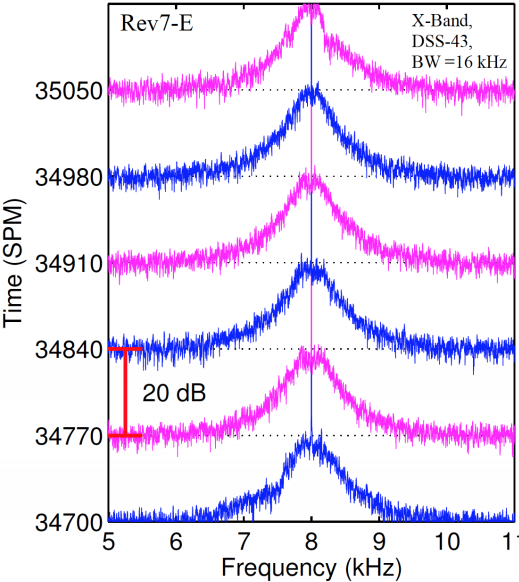
\includegraphics[width=\textwidth]{USER_7.png}
    	\caption{This is a caption}
    \end{subfigure}
    \begin{subfigure}[b]{0.49\textwidth}
        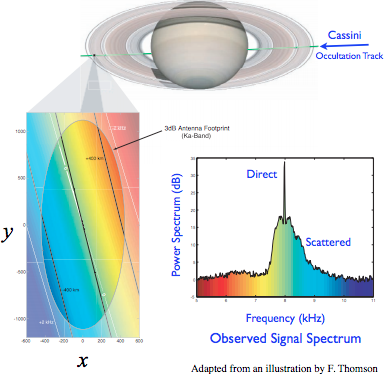
\includegraphics[width=\textwidth]{USER_7a.png}
        \caption{Yadda}
    \end{subfigure}
    \caption{Figures}
    \label{other_label_2}
\end{figure}
\noindent As an example, we consider the Cassini egress ring occultation Rev7-E. This image depicts a subset of the power spectra that was derived from the measured $(I_{m}(t), Q_{m}(t))$ samples. Both the direct-to-Earth and scattered signal components are visible. Each spectrum is searched for the frequency of its peak value near the center of the recording bandwidth. The peak is assumed to be the direct signal, but it can be scattered signal or noise where the ring has large optical depth. Least squares fitting of model spectra of sinusoidal signals to the measured spectral values around the peak can be used to refine the position of the peak. $f_{offset}(t)$ is then computed as the offset of the estimated peak frequency from the center of the recording bandwidth $(BW = 1\ \textrm{kHz})$. The first image on the next page depicts the $f_{offset}(t)$ curve computed for Rev-7E. This interval of time covers Rings C, B, and A, as well as free space. Free space is used to form the baseline. The profile is very noisy and almost random in the optically thick regions of Ring B, less noisy in Ring A, and much less noisy in Ring C, the Cassini Division, and outside Ring A. The plot of $f_{dp}(t) - f_{dr}(t)$ is the difference between the reconstructed and predicted Doppler shifts ($f_{dr}(t)$ is the reconstructed, and $f_{dp}(t)$ is the predicted). This accounts for the trend and a large fraction of $f_{offset}(t)$, but not necessary all of it. The difference is $f_{resid}(t) = f_{offset}(t) - \big(f_{dr}(t)-f_{dp}(t)\big)$. Coarser resolution was used to compute this curve to mitigate the effect of noise on the frequency estimates.
\noindent The most optically thick parts of Ring B yield unreliable estimates. Least squares fit of the reliable parts of the curve yield the heuristic estimate $\hat{f}_{resid}(t)$. Potential causes for $\hat{f}_{resid}(t)$ could be persistent error in the reconstructed spacecraft trajectory and other un-modeled long-term effects. This process is critical for ensuring that the phase of the calibrated signal $I_{c}(t)+iQ_{c}(t)$ is primarily due to ring material, instabilities in the USO reference phase, and any other unknown short-time effects that are no possible to correct for. Reliable computation of ring properties requires accurate determination of the free-space signal level $P_{0}(t)$ used to normalize the signal level through the occultation period. Direct measurement of $P_{0}(t)$ is only possible when the line-of-sight from Cassini to Earth is clear of all rings. Ring occultation observations were designed to allow measurements of $P_{0}(t)$ for a long interval of time exterior to Ring A. The geometry of some radial occultations allowed measurements of $P_{0}(t)$ in the gap between Ring C and Saturn's ionosphere. Least Squares Spline Fitting was used to obtain $P_{0}(t)$ estimates for the ring-free periods. The fitting yields $\hat{P}_{0}(t)$ during the entire observation period. The calibrated, diffraction-limited, complex ring transmittance is defined as:
\begin{equation}
\hat{T}_{R}(t) + i\hat{T}_{I}(t) = \frac{1}{\sqrt{\hat{P}_{0}(t)}}\big[I_{c}(t) + iQ_{c}(t)\big]
\end{equation}
\begin{figure}[htbp]
	\centering
	\begin{subfigure}[b]{0.49\textwidth}
    	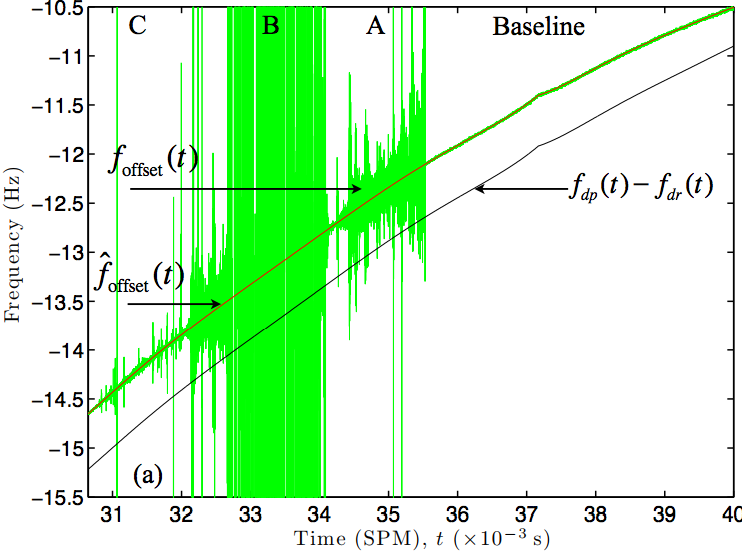
\includegraphics[width=\textwidth]{USER_8.png}
    	\caption{This is a caption}
    \end{subfigure}
    \begin{subfigure}[b]{0.49\textwidth}
        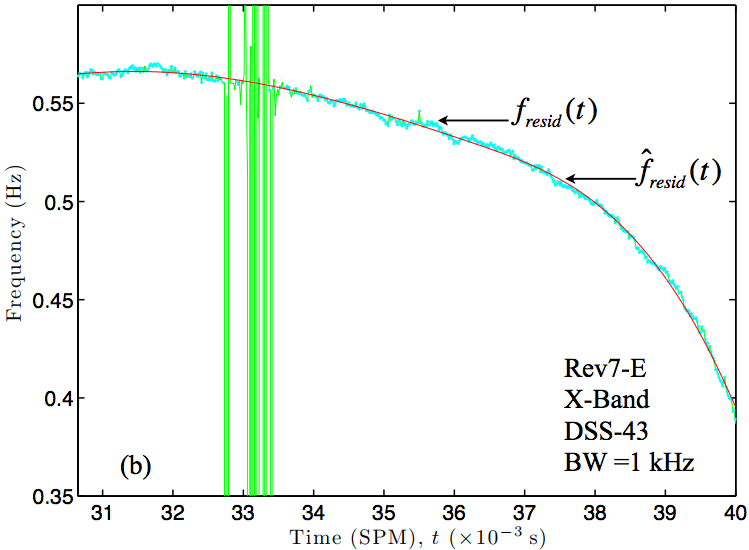
\includegraphics[width=\textwidth]{USER_8a.png}
        \caption{Yadda}
    \end{subfigure}
    \caption{Figures}
    \label{other_label}
\end{figure}
\noindent The calibrated data, $(\hat{T}_{R}(t),\hat{T}_{I}(t))$, form the starting point of all data analysis steps, including computation of optical depth profiles and scattered signal power spectra. There are both short and long term variations in $P_{0}(t)$. Long-term variations are caused by changes in the elevation angle of the DSN receiving antenna during the experiment, and systematic antenna pointing errors. Short-term fluctuations are typically caused by one or more terrestrial factors such as turbulence in the atmosphere, clouds, wind gusts (Causing mechanical vibrations of the receiving antenna), or fluctuations in the receiver gain or thermal noise. Complex samples of the calibrated data are uniformly spaced in time. The below figure depicts estimation of the free-space signal power $P_0(t)$ for Rev-7E.
\begin{figure}[htbp]
	\centering
	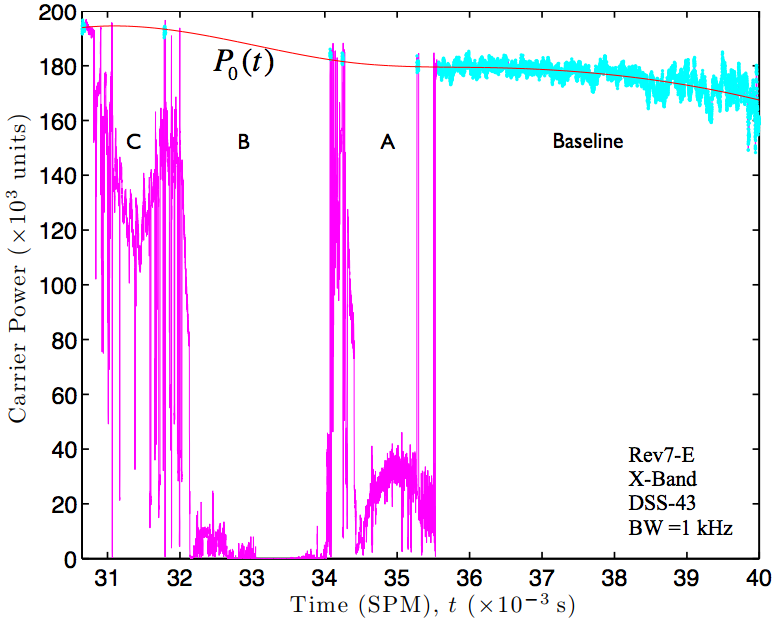
\includegraphics[width = 0.6\textwidth]{USER_9}
\end{figure}
The calculations are completed using a quasi-inertial Sun-centered reference frame with the light-time included. Ring accuracy of a few hundred meters is achievable, the primary source of Error being Saturn's pole orientation. The velocity of the ring-plane intercept point varies radially. Data sampled uniformly in time results in non-uniformly samples in ring radius. The following notation is used to denote calibrated complex ring transmittance samples at radius $\rho_0$ where the sampling is uniform in radius:
\begin{equation}
\hat{T}(\rho_0) = \hat{T}_{R}(\rho_0)+i\hat{T}_{I}(\rho_0)
\end{equation}

\noindent Radio occultations observations of planetary rings are diffraction limited. The measured $\hat{T}(\rho_0)$ and the true value of $T(\rho_0)$ differ because of diffraction effects. This difference can be related by the Fresnel Transform.

\begin{equation*}
    \hat{T}(\rho_0) = \frac{1-i}{2F}\int_{-\infty}^{\infty} T(\rho)e^{i\frac{\pi}{2}\big(\frac{\rho_0-\rho}{F}\big)^2}d\rho
\end{equation*}

\noindent Where $F$ is the Fresnel Scale of Diffraction, which depends on the observation wavelength and geometry. $T(\rho)$ is then:
\begin{equation}
T(\rho) = \frac{1+i}{2F}\int_{-\infty}^{\infty}\hat{T}(\rho_0)e^{-i\frac{\pi}{2}\big(\frac{\rho-\rho_0}{F}\big)^2}d\rho_{0}
\end{equation}
Quadratic phase approximations, sample resolution of $\hat{T}(\rho_0)$, and signal-to-noise in the measured values set limits on the recovery of $T(\rho)$. The normal optical depth profile and the phase-shift profile are computed as follows:
\begin{equation*}
    \tau(\rho) = -2\mu_{0}\ln\big(|X(\rho)|\big) \quad\quad\quad\quad \phi(\rho) = \tan^{-1}\bigg[\frac{X_{I}(\rho)}{X_{R}(\rho)}\bigg]
\end{equation*}
Where $\hat{X}(\rho_0) = \hat{T}(\rho_0) + \hat{n}(\rho_0)$ and $X(\rho) = T(\rho)+n(\rho) = X_{R}(\rho)+iX_{I}(\rho)$ denote the noisy measured and recovered values, respectively. $B$ is the ring opening angle, and $\mu_0 = \sin\big(|B|\big)$. Practical aspects of the implementation of the Fresnel inversion must be considered. The infinite range of $\rho_0$ must be replaced by the finite data window available. This sets of a limit of $\Delta R_{W} = 2\frac{F^2}{W}$ on the reconstructed resolution, where $W$ is the width of the window. To preserve information about structure on spatial scales equal to or larger than $\Delta R_{W}$, the diffraction-limited data $\hat{T}(\rho_0)$ must be sampled to or larger than twice the highest spatial frequency. This is the sampling theorem. The artificial truncation of the data for a finite width $W$ also creates problems in the reconstruction. To mitigate the sudden jump from positive to zero, a tapered window function that gradually decays to zero may be multiplied by the data. There is a degradation in the spatial resolution by up to a factor of $2$. The Effective resolution is defined below:
\begin{equation}
\Delta R_{eff} = -\sim 2\Delta R_{W}
\end{equation}
\begin{figure}
	\centering
	\begin{subfigure}[b]{0.49\textwidth}
    	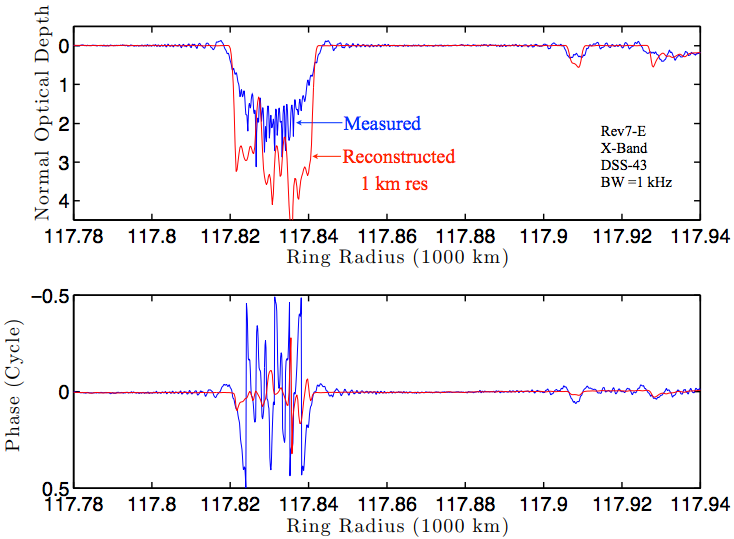
\includegraphics[width=\textwidth]{USER_10.png}
    	\caption{This is a caption}
    \end{subfigure}
    \begin{subfigure}[b]{0.49\textwidth}
        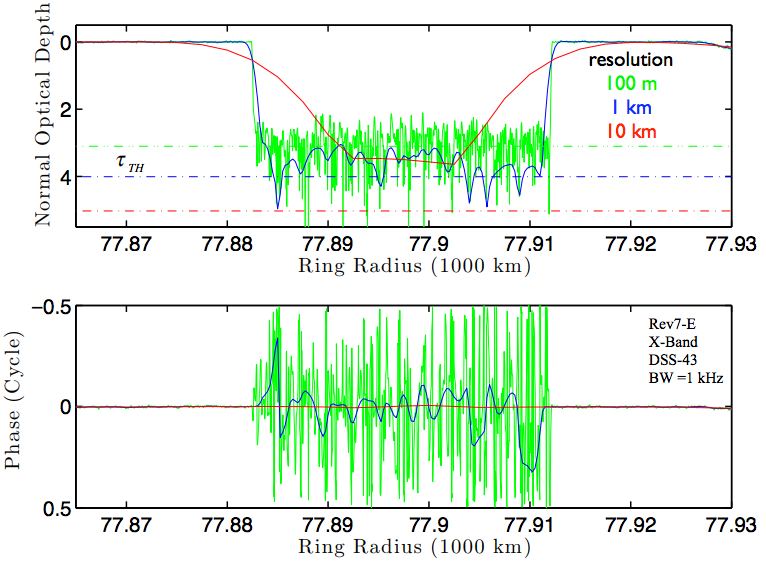
\includegraphics[width=\textwidth]{USER_11.png}
        \caption{Yadda}
    \end{subfigure}
    \caption{Figures}
    \label{label}
\end{figure}
These plots show the diffraction reconstruction of Rev-7E. The main ring feature is the Huygens Ringlet located within the Hugyens Gap. The blue curves represent the diffraction-limited X-band profiles $\hat{\tau}(\rho_0)$ and $\hat{\phi}(\rho_0)$ at 250 m resolution. The red curves depict $\tau(\rho)$ and $\phi(\rho)$ reconstructed using a processing resolution $\Delta R_{W} = 500$ m. The effective resolution is close to $1$ km. The best achievable radial resolution of a given features depends on the optical depth of the feature (The measurement SNR). Finer spatial resolution requires sampling at higher rates, which is noiser. Thermal noise is additive, and the SNR can be improved using coherent averaging. This reduces the resolution. There is thus a trade-off between finer resolution and uncertainty in the reconstructed profile. This is characterized by the threshold optical depth $\tau_{th}$. For a $70\%$ confidence interval:
\begin{equation}
\tau_{th} \approx -\mu_0\ln\big(1.205 P_N\big)
\end{equation}
Where $P_N$ is the average power of the additive noise. An estimate has the form:
\begin{equation}
\hat{P}_N = \frac{1}{SNR_0}\frac{\dot{\rho}_0}{\Delta R}
\end{equation}
Where $\Delta R = \Delta \rho_0$, the sample spacing of the diffraction-limited data, or $\Delta R_{eff}$, and $\dot{\rho}_0$ is the ring plane radial velocity of the ring intercept point. For Rev-7E, we have $B = -23.5^{\circ}$ and $\dot{\rho}_0 = 10 \textrm{km/s}$. The images below illustrate the trade-off. $\tau_{th}$ progressively increases from $3.1\rightarrow 4.0 \rightarrow 5.0$ as the resolution of $\Delta R_{eff}$ changes from $100\textrm{m}\rightarrow 1\textrm{km}\rightarrow 10\textrm{km}$. At $100$ m resolution, almost all structure in the ringlet is obscured by noise. The phase profile is essentially random. The ringlet edge is located with high accuracy, though. The absence of profile overshoot in the vicinity of transition to a zero value free-space optical depth indicates reliable reconstruction of the diffraction effects. At fine resolution, diffraction-limited data over a large radial interval is needed to compute the inverse Fresnel transform. 1 km resolution yields more reliable profiling of ringlet structure over the region where the recovered optical depth exceeds the corresponding threshold level, similarly for the phase profile. At 10 km, reliable measurements of the average optical depth of the ringlet is achieved but fine structure is lost. 

\subsubsection{Surface Scattering}

Bistatic radar (BSR) is the active probing of planetary surfaces by oblique reflection and scattering of microwave signals. This provides rms surface slopes and dielectric constant and density at scales comparable to the wavelengths used. A radio signal scatters off the surface and the echo is received on Earth. A direct signal is often sent concurrently. For typical spacecraft transmitters of $1-100$ Watts, surface echoes as low as $1$ Zeptowatt ($10^{-21}$ W) can be detected. Differential Doppler effects between the direct and reflected paths separates the received echo from the carrier. Dispersion of the echo provides a measure of the rms slope of the undulations. Where echo dispersion is small, the Doppler difference between the two primary paths can be used to infer large-scale topography. BSR is interested in amplitude, frequency, polarization, and time of the echo signal. Incremental power from an unresolved surface element is given by:
\begin{equation}
dP_{R} = \frac{P_T G_T}{4\pi R_{T}^2}\sigma\bigg(\frac{A_{R}}{4\pi R_{R}^2}\bigg)
\end{equation}
$P_T$ is the transmitted power, $G_T$ is the transmitting antenna gain in the direction of the surface element, $R_T$ is the distance from the transmitter to the surface element, $A_R$ is the effective area of the receiving antenna aperture, and $R_R$ is the distance from the surface element to the receiver. The bistatic cross section of the surface element is:
\begin{equation}
\sigma = \sigma_{0}dS
\end{equation}
Where $dS$ is the area of the surface element, and $\sigma_0$ is the specific radar cross section. $\sigma_0$ is assumed proportional to reflectivity, $\rho$, derived from Fresnel voltage reflection coefficients for horizontally and vertically polarized EM waves at a planar interface between free space and the planetary surface.

\begin{equation}
R_{HH} = \frac{\cos(\phi) - \sqrt{\epsilon-\sin^2(\phi)}}{\cos(\phi) + \sqrt{\epsilon - \sin^2(\phi)}} \quad \quad
R_{VV} = \frac{\epsilon \cos(\phi) - \sqrt{\epsilon - \sin^{2}(\phi)}}{\epsilon \cos(\phi) + \sqrt{\epsilon - \sin^2(\phi)}}
\end{equation}

\noindent Where $\epsilon$ is the dielectric constant of the surface material. The reflection coefficients for circularly polarized waves are:
\begin{equation}
R_{SC} = \frac{R_{VV}+R_{HH}}{2} \quad \quad
R_{OC} = \frac{R_{VV}-R_{HH}}{2}
\end{equation}
Where $R_{SC}$ is the voltage reflection coefficient for right-hand circular polarization (RCP) transmitted and received, and $R_{OC}$ is the coefficient for RCP transmitted and Left-Hand Circular Polarization (LCP) received.

\begin{wrapfigure}{l}{0.58\textwidth}
	\begin{center}
	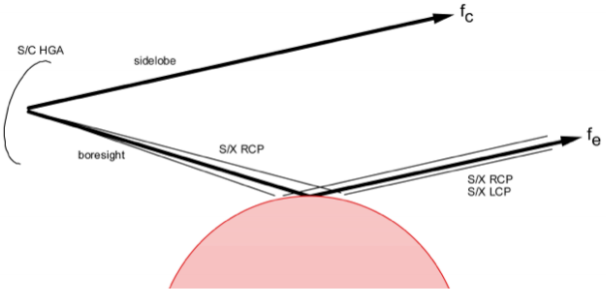
\includegraphics[width = 0.58\textwidth]{USER_12}
	\end{center}
\end{wrapfigure}
\noindent This image depicts the geometry of the experiment. If the transmitter is at $\mathbf{r}_{T}$ and the receiver is at $\mathbf{r}_{R}$, then the Doppler shift is the rate of change of the path length measured in wavelengths $\lambda$. 

\begin{equation}
f_{c} = \frac{d}{dt}\bigg(\frac{\norm{\mathbf{r}_{T}-\mathbf{r}_{R}}}{\lambda}\bigg)
\end{equation}

\noindent The Doppler shift for a signal reflected at the point $\mathbf{r}_{P}$ on a smooth target is:

\begin{equation}
f_{e} = \frac{d}{dt}\bigg(\frac{\norm{\mathbf{r}_{R} - \mathbf{r}_{P}}+\norm{\mathbf{r}_{T}-\mathbf{r}_{P}}}{\lambda}\bigg)
\end{equation}

\subsubsection{Fundamental Physics}

\noindent GWs are propagating, polarized gravitational fields (Ripples) in the curvature of space-time. Such waves are predicted by all relativistic theories of gravity. These waves are propagating space-time strain. They cause fractional frequency shifts of electromagnetic waves exchanged between separated test mass and cause differences in the rates at which separated clocks keep time. GWs are propagating solutions of Einstein's Field Equations. They propagate at the speed of light, carry energy and momentum, are transverse to the propagation direction, and have two independent polarization states. GWs couple very weakly to matter. Only massive sources undergoing extreme dynamics could generate detectable waves. This means GWs preserve information about the deep interiors of high gravity/high velocity objects. The Doppler tracking method measures the Earth-Spacecraft fractional Doppler shift, $\frac{\delta f}{f_0}$, where $\delta f$ is the Doppler shift and $f_0$ is the radio link's carrier frequency. The Doppler shifts due to Earth and spacecraft motion must be removed, the ODP is used for this. The difference between observed sky frequency and predicted sky frequency is called the residual frequency. Dividing this by the link center frequency, $f_0$, gives the value of $y$. The GW signature in the time series is:
\begin{equation}
y_{signal} = \frac{\mu-1}{2}Y\big(t\big)- \mu Y\big(t-\frac{1+\mu}{2}T_2\big)+\frac{1+\mu}{2}Y\big(t-T_2\big)
\end{equation}
Where $\mu$ is the cosine of the angle between the Earth-spacecraft line and the propagation vector of the GW, $Y(t) = \frac{\hat{\mathbf{n}}\cdot \mathbf{h}}{1-\mu^2}$, where $\hat{\mathbf{n}}$ is the unit vector from Earth to the spacecraft, and $\mathbf{h}$ is the first order metric perturbation of the Earth. This response of the Dopple to a GW excitation is interpreted as due to the GW striking the Earth, the GW striking the spacecraft (at a delayed time), and the original Earth buffeting transponded back to the Earth a two-way light time later. The parametrized Post Newtonian (PPN) formalism is a formal approach to compare metric theories of relativistic gravity with each other and with experiments. The PPN approach is simplest in slow motion, weak field limits. In the inner solar system, $\norm{\mathbf{v}}$, the velocity of an object with respect to the center, is usually less than 30 km/sec. So $\frac{v^2}{c^2} \approx 10^{-8}$, and this is considered slow. At the surface of the Sun, $\frac{U}{c^2}$, where $U$ is the Newtonian potential, is on the order of $10^{-6}$. Everywhere else in the solar system is much less. So, the PPN is simple for the solar system. The parameter $\gamma$ characterizes the space-time curvature produced per unit mass. In the Theory of General Relativity (GR), $\gamma=1$. $\gamma$ has been measured by measurements of the range and range rate between Earth and distant spacecraft as the line between the two passes close to the Sun. Non-Newtonian contributions from the Sun's curving of space-time are created. 
\begin{equation}
\Delta t = \frac{1+\gamma}{2}\bigg(240 - 20\frac{\ln\bigg(\frac{b^2}{r_{sun}^2}\bigg)}{\frac{r}{1\textrm{AU}}}\bigg)
\end{equation}
Where $b$ is the impact parameter of the ray, $r_{Sun}$ is the solar radius, and $r$ is the range to the spacecraft. Viking range observations had $\gamma=1$ to one part in $1000$. For Cassini, the radial velocity was measured. Due to motions of the spacecraft and the Earth during the conjunction, the closest approach distance changes with time, inducing a relative frequency shift of the carrier:

\begin{equation}
\frac{\Delta v}{v} = -\frac{d\Delta t}{dt} = -4(1+\gamma)\frac{GM}{bc^3}\frac{db}{dt} = -2\mu s(1+\gamma)\frac{1}{b}\frac{db}{dt}
\end{equation}
In 2002, Cassini was 7.4 AU from the sun. $\frac{db}{dt}$ was close to being determined by the Earth orbital velocity, and the relative frequency shift was on the order of $10^{-9}$. Radio signals are strongly affected by the solar corona. The refractive index of the spectrum is inversely proportional to the square of the carrier frequency, and thus $X$ and $Ka-$band signals were nearly completely free of these plasma effects. 
%
\section{Theory of Radio Occultation by Saturn's Rings - Marouf et. al.}
%
\subsection{Abstract}
\noindent Rings may be studied by the perturbations they introduce in the spectrum of radio signals transmitted through them by a spacecraft during occultations. Two separate signal components are identified in a perturbed spectrum: A sinusoidal component that remains coherent with the incident signal but is reduced in intensity and possibly changed in phase, and a Doppler-broadened incoherent component whose spectral shape and strength are determined by occultation geometry and the radial variation of the near-forward radar cross section of illuminated ringlets. When the occultation geometry is optimized, contributions of an individual ringlet to a perturbed spectrum can be identified with radial resolution of a few kilometers for the coherent component and a few hundred kilometers for the incoherent one. If the particles are of known material and form a narrow size distribution with radii greater than severals tens of centimeters, then estimates of both optical depth and radar cross section of a ringlet at $3.6\ \textrm{cm}-\lambda$ allow separation of its aerial density and particle size. This separation is shown for radii $\leq 10\ \textrm{cm}$ from differential effects on the coherent signal parameters at $3.6$ and $13$ cm. For the general case of a broad size distribution modeled by a power law, the absence of differential effects on the coherent signal binds the minimum size to be $\geq 10\ \textrm{cm}$. Here, the radius inferred from an estimate of the radar cross section represents an equivalent radius. Detection of differential coherent signal extinction determines an upper bound on the minimum size and a lower bound on the power index, assuming water-ice particles. These bounds and the inferred equivalent size constrain the size distribution at both small and large ends.
\subsection{Introduction}
\noindent Radio occultation of planetary rings involves a radio signal sent from a spacecraft to Earth being intercepted by the rings. In free space the spacecraft modulates a continuous sinusoidal carrier signal whose frequency, phase, and intensity can be estimated upon reception on Earth. When the radio path is interrupted by the rings, these values may be perturbed. Voyager 1 was the first spacecraft to conduct ring occultation experiments when it flew by Jupiter on March 5, 1979, and later Saturn on November 12, 1980. The Jovian rings were undetectable, but Saturn's were. Saturn's rings have been studied since the $17^{th}$ century. Significant improvement in spatial resolution over Earth-based observations came in 1979 when Pioneer made a fly-by of Saturn's rings. Photometric observations were not supportive of simple homogeneous ring models. Voyager 1 confirmed this by revealing intricate radial structure. Inferring physical structure by averaging observations over a large ring area may result in inaccurate or misleading interpretations. The geometry of occultations is rather strange. The line of sight between transmitter and receiver passes through the material. The highly directive spacecraft antenna restricts viewing geometry to scattering directions close to the exact forward direction, that is, to phase angles within a few degrees of $180^{\circ}$. The received signal retains the original incident ray as one distinct component but reduced in intensity and possibly changed in phase. This is the coherent signal. A ring particle larger than the wavelength of the signal intercepts from the incident wave a total power that is proportional to its geometrical cross-sectional area but re-scatters the power in the near-forward direction in proportion to the square of its cross-sectional area. This is a consequence of the dominance of diffraction on near-forward scattering. This behavior does not hold for mono-static radar geometries, or bi-static geometries away from the forward diffraction lobe. The rings will first be treated as a Doppler-spread radar target composed of an ensemble of discrete scatterers. The formulation of the received signal as a random-phasor-sum process is carried out following radar theory. Treating the average effects of the ring material on the direct ray in terms of the effects of a fictitious dielectric medium, the equivalent refractive index of the medium will be obtained. The direct ray is actually associated with finite ring area of size roughly equal to the size of the first Fresnel zone, so the complex phase of the coherent signal that is obtained from this equivalent refractive index requires the width of the ringlet to be much larger than the Fresnel zone. The analysis is generalized for ringlets of arbitrary size. When the width is such that two adjacent rays are differentially perturbed in phase, ray bending that causes focusing or defocusing of the coherent signal may result. Voyager 1 has revealed many diffractive effects. They usually occur on the boundaries with areas in which the material is substantially absent. This implies edges that are sharp on the scale of the Fresnel zone. In the terminology of the transfer equation through discrete random media, the coherent signal is a generalization of the reduced intensity component, although the monochromatic nature of the illumination introduces additional constraints. The other component arises from waves scattering at least once on a ring particle and is the diffuse component. The incoherent component of the received signal is the diffuse component that arises from waves scattering off of ring particles at least once. The Doppler shift from the relative motion of the ring particles with the spacecraft spread the power of the incoherent signal in frequency. This allows separation of this signal in the frequency spectrum of the total received signal from that of the coherent signal. The frequency spectrum of the incoherent signal is derived as the Fourier transform of the covariance function of the random phasor sum process. This will show that it is affected by both occultation geometry and the scattering cross-section of the rings. Voyager 1 will be used to show the impact of trajectory choice on the degree of alignment of contours of constant Doppler shift on the ring plane with boundaries of individual ringlets and on the ability to recover the radial variation of the radar cross section of a given ringlet. Lastly the problem of inference of the particle size distribution of a ringlet from the measurements under the constraints of the real world are addressed. The main assumption is that the ring material is made of nearly lossless water-ice. Silicate-type material is also used to demonstrate the implications of finite particle loss.
\subsubsection{Received Signal}
\noindent The center of mass of Saturn, which is assumed to be the center of figure, is chosen as the origin. Saturn's ring plane coincides with its equatorial plane, and this defines the $xy-$plane. $\hat{\mathbf{z}}$ is chosen parallel to the spin axis such that Saturn spins counterclockwise about it. We assume that the incident waves are plane waves.
\begin{wrapfigure}{l}{0.45\textwidth}
	\centering
	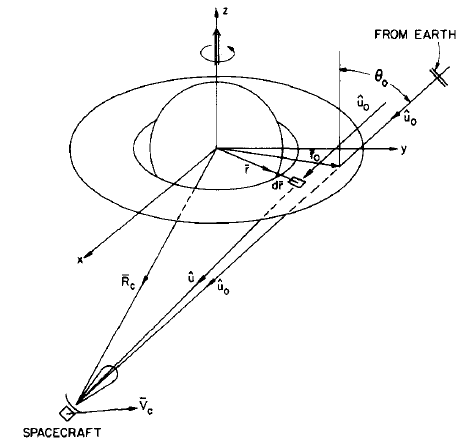
\includegraphics[width = 0.45\textwidth]{Marouf81_1}
\end{wrapfigure}
\noindent Let $\hat{\mathbf{z}}_{E}$ be the normalized spin axis of the Earth (The unit vector pointing from Earth's core to the North Pole). Let $\mathbf{x}_{E}$ be the unit vector pointing from the core of the Earth to the equator at the prime meridian, and $\hat{\mathbf{y}}_{E} = \hat{\mathbf{z}}_{E}\times \hat{\mathbf{x}}_{E}$. Let $\mathbf{u}_{0}$ be the position of the spacecraft. Note that $\cos^{-1}\big(\hat{\mathbf{z}}\cdot\hat{\mathbf{z}}_{E}\big)$ is the angle between Earth's spin axis and Saturn's spin axis. We define $\hat{\mathbf{y}} = \frac{\hat{\mathbf{z}}\times \mathbf{u}_{0}}{\norm{\hat{\mathbf{z}}\times \mathbf{u}_{0}}}$. $\hat{\mathbf{z}}$ and $\mathbf{u}_{0}$ are never parallel, so $\hat{\mathbf{y}}$ is well defined. Finally, $\hat{\mathbf{x}} = \hat{\mathbf{y}}\times \hat{\mathbf{z}}$. It will be often useful to convert between Earth based and Saturn based systems. This is done via a three-dimensional rotation matrix. The line from Earth to the spacecraft lies parallel to the $xz-$plane. The angle between the $xy-$plane and the plane that contains the Earth-Spacecraft line and the center of Saturn is denoted $\theta_{0}$. The ring opening angle is defined as $\psi = \frac{\pi}{2} - \theta_{0}$. As both the Earth and Saturn orbit the sun, the value of $\psi$ varies $0\leq |\psi| \leq \frac{3}{20}\pi = 27^{\circ}$. We use $\hat{\mathbf{u}}_{0}$ to denote $\frac{\mathbf{u}_{0}}{\norm{\mathbf{u}_{0}}}$. The incident wave interacts with the material of the rings, scattering it in all spatial directions. Some of the energy transmitted through the rings is received on Earth. In the real world, the Earth and the spacecraft move with respect to Saturn over time. We use $\overline{\mathbf{R}}_{c}(t)$ to denote the position vector of the spacecraft with respect to Saturn over time, and $\overline{\mathbf{V}}_{c} = \frac{d \overline{\mathbf{R}}_{c}}{dt}$ to denote the velocity vector of the spacecraft with respect to Saturn. The vector $\overline{\mathbf{r}}_{0}$ represents the point of intersection with the Earth-Spacecraft line and the $xy-$plane (The ring plane). This point is called the ring intercept point. Because the receiving antenna has a finite beamwidth, a region of finite extent will contribute to the received signal at any value of $\overline{\mathbf{r}}_{0}$. An example is a small region of area $d\overline{r}$ centered at $\overline{\mathbf{r}}$ that scatters energy towards the receiving antenna. If $\overline{\mathbf{R}}_{E}$ is the position vector of Earth from Saturn, then this energy will travel along the vector $\hat{\mathbf{u}}\big(\overline{\mathbf{r}}\big) = \frac{\overline{\mathbf{R}}_{E}-\overline{\mathbf{r}}}{\norm{\overline{\mathbf{R}}_{E}-\overline{\mathbf{r}}}}$. This contribution will be weighed by the gain $G(\hat{\mathbf{u}})$ of the receiving antenna in the direction $\hat{\mathbf{u}}\big(\overline{\mathbf{r}}\big)$. 

\subsection{Model}

We assume that a ring particle at position $\overline{\mathbf{R}} = (\overline{r},z)$ moves in a Keplerian orbit about Saturn with a dominant velocity component $\overline{\mathbf{V}}\big(\overline{r}\big)$ that is equal to the circular velocity of a body of negligible mass rotating in Saturn's gravity field at a radius $r$. If $\hat{\mathbf{u}}_{r}$ is the radial unit vector at $\overline{r}$ and $\hat{\mathbf{u}}_{\phi} = \frac{\hat{\mathbf{z}}\times \hat{\mathbf{u}}_{r}}{\norm{\hat{\mathbf{z}}\times \hat{\mathbf{u}}_{r}}}$, then:

\begin{equation}
\overline{\mathbf{V}}\big(\overline{r}\big) = \sqrt{\frac{GM}{r}}\hat{\mathbf{u}}_{\phi}
\end{equation}

Where $G$ is the universal gravitational constant and $M$ is Saturn's mass. This may be perturbed by a random component $\overset{\sim}{\mathbf{V}}\big(\overline{\mathbf{R}}\big)$. The time it takes for light to travel from a particle at $\overline{\mathbf{R}}$ to the spacecraft at $\overline{\mathbf{R}}_{c}$ is:

\begin{equation}
\tau = \frac{\norm{\overline{\mathbf{R}}_{c}-\overline{\mathbf{R}}}}{c}
\end{equation}

\noindent Where $c$ is the speed of light in vacuum. Because the change in $\overline{\mathbf{R}}$ is small over the time scale of $\tau$, the signal scattered to the receiver from a signal particle normalized to the free-space received signal takes the form:

\begin{equation}
E_{p} = G(\hat{\mathbf{u}})A(\hat{\mathbf{u}},\hat{\mathbf{u}}_{0};\overline{\mathbf{R}},\overline{\gamma})\frac{e^{ik(\overline{\mathbf{R}}_{c}-\overline{\mathbf{R}})\cdot (\hat{\mathbf{u}}-\hat{\mathbf{u}}_{0})}}{k\norm{\overline{\mathbf{R}}_{c}-\overline{\mathbf{R}}}}
\end{equation}

\noindent Where $k = \frac{2\pi}{\lambda}$, where $\lambda$ is the wavelength of the incident wave, and $A$ is the scattering amplitude. $A$ represents one of four possible combinations of two orthogonal polariztions of the transmitter and receiver. Its value is determinded by the size, shape, material, and orientation of the particle. $\overline{\gamma}$ symbolizes the dependence of each of these parameters. We assume that $A$ is radially symmetric. The relative motion of the spacecraft and particle causes the instantaneous angular frequency $\Omega_{D}\big(\overline{\mathbf{R}}\big)$ of the normalized signal to differ from zero. These are the Doppler shifts.

\begin{equation}
\Omega_{D}\big(\overline{\mathbf{R}}\big) = -k\big(\overline{\mathbf{V}_{c}} - \overline{\mathbf{V}}-\overset{\sim}{\mathbf{V}}\big)\cdot \big(\hat{\mathbf{u}} - \hat{\mathbf{u}}_{0}\big)
\end{equation}

The total normalized received signal is obtained by summing the contributions of individual particles and the incident signal:

\begin{equation}
E = 1+\sum_{p} E_{p}
\end{equation}

Where $p$ is the set of particles within the field of view of the spacecraft antenna. This equation assumes that the particles are non-interacting. That is, each particles receives the full illumination of the incident wave and the particles are widely separated so that the fraction of the unit ring volume occupied by the particles is much less than $1$. Evidence in support of volume fractions in the range of $0.01$ or less have been reported for Saturn's rings. 

\subsection{Statistics}

The received signal $E$ is a random process for two reasons. The random distribution of the particles will result in a randomization of the phases of the individual scattered signals, except for the exact forward direction. Second, the possible random size, shape, material, and orientation of the ring particles could randomize the $E_{p}$ components. For loosely packed rings, the positions of the particles can be modelled by a Poisson Law. The probability of finding $N$ particles within a small element of ring volume $dv$ centered at $(\overline{r},z)$ is:

\begin{equation}
P_{N} = \frac{\big(n(\overline{r},z)dv\big)^N}{N!}e^{-n(\overline{r},z)dv}
\end{equation}

This model is equivalent to the assumption that a particle can exist anywhere in $dv$ irrespective of other particles. This cannot be true for particles of finite size, but is approximate when the average distance between particles is large compared to their size. In this equation, $n(\overline{r},z)$ is the average number density, which is not a random function. It is a function of $z$. If the number density is greatest at the equatorial plane and gradually decreases as one moves away from it, we may model this with a Gaussian:

\begin{equation}
n(\overline{r},z) = n(r)e^{-\frac{z^2}{2d^2}}
\end{equation}

Where $d$ is a measure of the rings thickness. A more common density profile is:

\begin{equation}
n(\overline{r},z) = \begin{cases} n(r), & 0\leq |z| \leq d \\ 0, & d<|z|\end{cases}
\end{equation}

That is, the rings are a slab of finite thickness $d$. Occultation observations wish to measure the average of $\overline{\gamma}$ and the value of $n(r)d$. In the case of a monolayer of particles, the column density $(n(r)\cdot d)$ degenerates to the average number of particles per unit ring area $n_{S}(r)$. The Poisson law could still hold if the fraction of area occupied by particles is small. Radio occultation experiments wish to obtain statistical averages of $\overline{\gamma}$ and $n(r)d$. The scattering amplitude $A$ of a single particle is difficult to compute. For the case of a homogeneous collection of dielectric spheres, the particle radius $a$ is the only component of $\overline{\gamma}$ whose probability function $p(\overline{\gamma})$ now represents the particle size distribution. This value is presumed to be determined by the physical process that created the ring particles. A ring originating from fragmentation of larger bodies is expected to have a power law size distribution of the form:
\begin{equation}
p(a) = \begin{cases} \gamma_{1}a^{-q}, & a_{min}\leq a \leq a_{max} \\ 0, & Otherwise\end{cases}
\end{equation}
Where $3\leq q \leq 4$ and $\gamma_{1}$ is a constant. Upper bounds on particle sizes are set by collisional fragmentations which allows particles to be tens of kilometers in radius. Radiation pressure sets a lower bound, as extremely small particles would be blasted away. A distribution specified by Cuzzi and Pollack is specified in terms of the effective size $a_{e}$ and effective variance $\sigma_{e}$:
\begin{align}
a_{e} &= \frac{\langle \pi a^3\rangle}{\langle \pi a^2\rangle}\\
\sigma_{e} &= \frac{\langle \pi a^2(1-\frac{a}{a_{e}})^2\rangle}{\langle \pi a^2\rangle}\\
p(a)da &= \gamma_{2}\bigg(\frac{a}{a_{e}}\sigma_{e}\bigg)^{\frac{1-3\sigma_{e}}{\sigma_{e}}}e^{-\frac{a}{a_{e}}\sigma_{e}}d\bigg(\frac{a}{a_{e}}\sigma_{e}\bigg)
\end{align}
Here, $\gamma_{2} = \Gamma^{-1}\big(\frac{1-2\sigma_{e}}{\sigma_{e}}\big)$. The received signal is assumed to be Gaussian if the random phasor sum is over many independent events. 

\subsection{Coherent Signal}

Coherent interference among the individual scattered waves in the random sum occurs for scattering directions near the forward-scattering direction. The coherent signal at any time $t$ is:

\begin{equation}
\langle E \rangle = A_{c}e^{i\phi_{c}} = 1+\int_{Rings}G(\hat{\mathbf{u}})n(\overline{\mathbf{R}})A(\hat{\mathbf{u}},\hat{\mathbf{u}}_{0};\overline{\mathbf{R}})\frac{e^{ik(\overline{\mathbf{R}}_{c}-\overline{\mathbf{R}})\cdot(\hat{\mathbf{u}}-\hat{\mathbf{u}}_{0}})}{k\norm{\overline{\mathbf{R}}_{c}-\overline{\mathbf{R}}}}d\overline{\mathbf{R}}
\end{equation}

Where the integration is over the total ring volume and $A$ is the average single-particle scattering amplitude:

\begin{equation}
A(\hat{\mathbf{u}},\hat{\mathbf{u}}_{0};\overline{\mathbf{R}}) = \int A(\hat{\mathbf{u}},\hat{\mathbf{u}}_{0};\overline{\mathbf{R}},\overline{\gamma})p(\overline{\gamma})d\overline{\gamma}
\end{equation}

The model of signal scattering by a fictitious medium of refractive index $m(\overline{\mathbf{R}})$ occupying the ring volume is worth exploring. For the scalar case, the scattered field normalized by a free-space incident field of the form $e^{ik\hat{\mathbf{u}}_{0}\cdot \overline{\mathbf{R}}-i\omega_{0}t}$ and received with aperture weight $G(\hat{\mathbf{u}})$ is:

\begin{equation}
U(\overline{\mathbf{R}}_{c}) = 1+\int k^2[m^2(\overline{\mathbf{R}}) - 1]G(u)\frac{e^{ik(\overline{\mathbf{R}}_{c}-\overline{\mathbf{R}})\cdot(\hat{\mathbf{u}}-\hat{\mathbf{u}}_{0})}}{4\pi \norm{\overline{\mathbf{R}}_{c}-\overline{\mathbf{R}}}}U(\overline{\mathbf{R}})d\overline{\mathbf{R}}
\end{equation}

Where $U(\overline{\mathbf{R}})$ is the normalized unknown field within the slab. For very tenuous ring structure, $m\approx 1$. So we have $m^2-1 = (m+1)(m-1) \approx = 2(m-1) \approx = A(0)n\frac{4\pi}{k^3}$, where $A(0)$ is the average exact forward-scattering amplitude. 
%
\section{Profiling Saturn's Rings by Radio Occultation - Marouf et. al.}
\section{Geometry of the Saturn System from the July 3, 1989 Occultation 28 Sgr and Voyager Observations}
\section{Characteristics of Different Smoothing Windows}
\begin{wrapfigure}{l}{0.4\textwidth}
	\begin{center}
	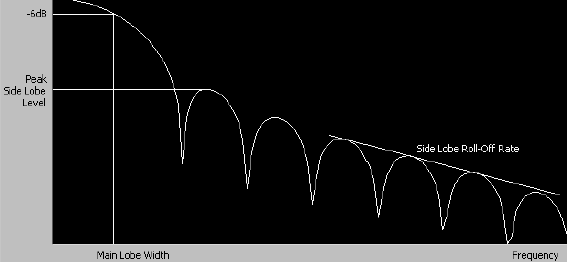
\includegraphics[width = 0.4\textwidth]{CDSW_1}
	\end{center}
\end{wrapfigure}
\noindent A plot of a smoothing window shows that the frequency characteristic of the smoothing window is a continuous spectrum with a main lobe and several side lobes. The center of the main lobe of a smoothing window occurs at each frequency component of the time-domain signal. The unit of measure for the main lobe width is FFT bins or frequency lines. This width limits the frequency resolution of the windowed signal. The ability to distinguish two closely spaced frequency components increases as the main lobe narrows. However, the window energy spreads into the side lobes, increasing spectral leakage and decreasing amplitude accuracy. There is a trade-off between amplitude accuracy and spectral resolution. Side lobe characteristics of the smoothing window directly affect the extent to which adjacent frequency components leak into adjacent frequency bins. The side lobe response of a strong sinusoidal signal can overpower the main lobe response of a nearby weak sinusoidal signal. Maximum side lobe level and lobe roll-off-rate characterize the sides lobes of a smoothing window. For the remainder of this article, $N$ is the window length, $n=0,1,2,\hdots, N-1$, and $w(n)$ is the window value at $n$.
\subsection{Rectangular}
\noindent The rectangular window is defined as $w(n) = 1$ for $n=0,1,2,\hdots, N-1$, where $N$ is the length of the window. This window just truncates the signal to within a finite time interval and has the highest amount of spectral leakage, but is the easiest to compute. It is useful for analyzing transients that have a shorter duration than that of the window. Transients are signals that exist only for a short duration of time. It is also used in order tracking, where the effective sampling rate is proportional to the speed of the shaft in rotating machines. 

\subsection{Bohman}
\noindent The Bohman window is defined by the following:
\begin{equation}
w(n) = \bigg(1-\frac{|n-\frac{N}{2}|}{\frac{N}{2}}\bigg)\cos\bigg(\pi\frac{|n-\frac{N}{2}|}{\frac{N}{2}}\bigg)+\frac{1}{\pi}\sin\bigg(\pi\frac{|n-\frac{N}{2}|}{\frac{N}{2}}\bigg)
\end{equation}

\subsection{Hanning}
\noindent The Hanning window has a shape similar to that of half a cycle of a cosine wave.
\begin{equation}
w(n) = \frac{1}{2}\bigg(1-\cos(\frac{2\pi n}{N})\bigg)
\end{equation}

\noindent This is useful for analyzing transients longer than the time duration of the window and for general-purpose applications.

\subsection{Hamming}
The Hamming window is a modification of the Hanning window.

\begin{equation}
w(n) = 0.54 - 0.46\cos(\frac{2\pi n}{N})
\end{equation}
\noindent In the time-domain, the Hamming window does not get as close to zero near the edges.
\subsection{Kaiser-Bessel}
The Kaiser-Bessel window is a flexible window whose shape can be modified by the value $\alpha$. This can control spectral leakage.
\begin{equation}
w(n) = \begin{cases} \frac{I_{0}\bigg(\alpha \pi \sqrt{1-\big(\frac{2n}{N-1}-1\big)^2}\bigg)}{I_{0}(\pi\alpha)}, & 0 \leq n \leq N-1\\ 0, & n>N-1\end{cases}
\end{equation}
\noindent As $\alpha \rightarrow 0$, $w$ tends to the rectangular window. As $\alpha \rightarrow \infty$, $w$ tends to a finite delta function. 
\subsection{Low Sidelobe}
\noindent The Low Sidelobe window reduces the level of the side lobes at the cost of broadening the main lobe. 
\begin{equation}
w(n) = \sum_{k=0}6{4} (-1)^{k}a_{k}\cos(k\frac{2\pi n}{N})
\end{equation}
\noindent Where $a_1 = 0.47149, a_{2} = 0.17553, a_{3} = 0.028497, a_{4} = 0.0012613$.
\subsection{Bartlett Window}
\noindent The Bartlett window is a triangle.
\begin{equation}
w(n) = 1-\big|\frac{2n-N}{N}\big|
\end{equation}
\subsection{Modified Bartlett-Hanning}
\noindent The Modified Bartlett-Hanning window is an integration of the Bartlett and Hanning windows. 
\begin{equation}
w(n) = 0.62-0.48\big|\frac{n}{N}-\frac{1}{2}\big|+0.38\cos\big(2\pi(\frac{n}{N}-\frac{1}{2})\big)
\end{equation}
\subsection{Parzen}
\noindent The Parzen window is a piecewise cubic curve obtained by convolving two triangles of half length or four rectangles of one-fourth length.
\begin{equation}
w(n) = \begin{cases} 1 - 6\big(\frac{n-\frac{N}{2}}{\frac{N}{2}}\big)^2+6\big(\frac{|n-\frac{N}{2}|}{\frac{N}{2}}\big)^3 & 0 \leq |n-\frac{N}{2}| \leq \frac{N}{4} \\ z\big(1 - \frac{|n-\frac{N}{2}|}{\frac{N}{2}}\big)^3 & \frac{N}{4} \leq |n-\frac{N}{2}|\leq \frac{N}{2} \end{cases}
\end{equation}
\subsection{Welch Window}
The Welch window is a continuous polynomial window:
\begin{equation}
w(n) = 1-\big(\frac{n-\frac{N}{2}}{\frac{N}{2}}\big)^2
\end{equation}
\subsection{Flat Top Window}
\noindent The flat top window has the best amplitude accuracy of all of the smoothing windows at $\pm 0.02$ dB for signals exactly between integral cycles. Due to the wide main lobe, it has poor frequency resolution. 
\begin{equation}
w(n) = \sum_{k=0}^{4} (-1)^{k}a_{k}\cos(k\frac{2\pi n}{N})
\end{equation}
\noindent Where $a_{0} = 0.21557, a_{1} = 0.41663, a_{2} = 0.277263, a_{3} = 0.08357, a_{4} = 0.0069473$. It is most useful in accurately measuring the amplitude of single frequency components with little nearby spectral energy in the signal.
\subsection{Exponential Window}
The exponential window is a decaying exponential.
\begin{equation}
w(n) = e^{\frac{n\ln(f)}{N-1}} = f^{\frac{n}{N-1}}
\end{equation}
\noindent Where $f$ is the final (Cut-off) value. This is useful for analyzing transient response signals whose duration is longer than the length of the window. It damps the end of the signal, ensuring that the signal fully decays by the end of the sample block. 
\subsection{Blackman Window}
\begin{equation}
w(n) = 0.42 - 0.5\cos(\frac{2\pi n}{N}) + 0.08\cos(\frac{4 \pi n}{N})
\end{equation}
\noindent The Blackman window is useful for single tone measurement because it has a low maximum side lobe level and a high side lobe roll-off rate.
\subsection{Exact Blackman Window}
\begin{equation}
w(n) = \frac{7938}{18608} - \frac{9240}{18608}\cos(\frac{2\pi n}{N}) + \frac{1430}{18608}\cos(\frac{4\pi n}{N})
\end{equation}
\noindent This is useful for single tone measurement. It has a lower main lobe width and a lower maximum side lobe level than the Blackman window. It has a higher side lobe roll-off rate, however.
\subsection{Blackman-Harris Window}
\noindent The Blackman-Harris window is a modification of the Blackman window.
\begin{equation}
w(n) = 0.422323 - 0.49755\cos(\frac{2\pi n}{N}) + 0.07922\cos(\frac{4\pi n}{N})
\end{equation}
\noindent This window is also useful for single tone measurement. It has a wider main lobe and a lower maximum side lobe level than the Exact Blackman Window.
\subsection{Blackman-Nuttal Window}
\noindent The Blackman-Nuttal window is a modified version of the Exact Blackman Window. 
\begin{equation}
w(n) = 0.3635819 - 0.4891775\cos(\frac{2\pi n}{N}) + 0.1365995\cos(\frac{4\pi n}{N}) - 0.0106411\cos(\frac{6\pi n}{N})
\end{equation}
\noindent This is good for single tone measurement. It has the widest main lobe and the lowest maximum side lobe level.
\begin{figure}[htbp]
  \centering
{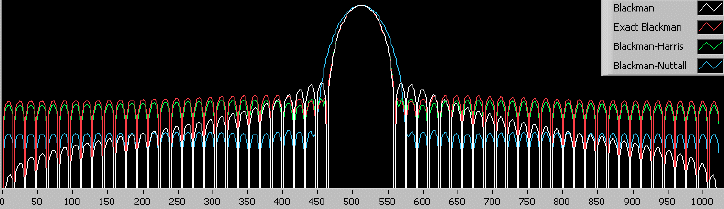
\includegraphics[scale=0.65]{CDSW_2}}
\end{figure}
\subsection{General Cosine Window}
\begin{equation}
w(n) = \sum_{k=0}^{m-1} (-1)^{k}a_{k}\cos(k\frac{2\pi n}{N})
\end{equation}
\noindent Where $m$ is the number of coefficients being used. The Hanning, Hamming, Flat Top Window, and Blackman Windows are special cases of this.
\subsection{Cosine Tapered Window}
\begin{equation}
w(n) = \begin{cases} \frac{1}{2}\big(1-\cos(\frac{\pi n}{m})\big) & n=0,1,2,\hdots, m-1\\ \frac{1}{2}\big(1-\cos(\frac{\pi}{m}(N-n-1))\big) & n = N-m, \hdots, N-1
\end{cases}
\end{equation}
\noindent Where $r = \floor{\frac{Nr}{2}}$, where $r$ is the ratio of the total length of the tapered section to the whole signal length. This window smoothly sets the data to zero at the boundaries without reducing significantly the processing gain of the windowed transform.
\subsection{Gaussian Window}
\begin{equation}
w(n) = e^{-\frac{(n-m)^2}{2(\sigma N)^2}}
\end{equation}
\noindent Where $m = \frac{N-1}{2}$, and $\sigma$ is the standard deviation of the window. This window is useful for time-frequency analysis because the Fourier Transform and the derivative of the Gaussian window are both Gaussian functions. A short-time Fourier Transform with a Gaussian window is a Gabor transform.
\subsection{Dolph-Chebyshev Window}
\begin{equation}
w(n) = \frac{1}{N}\bigg[s+2\sum_{k=1}^{\floor{\frac{N-1}{2}}}c_{N-1}\bigg(t_{0}\cos(\frac{k\pi}{N})\bigg)\cos(\frac{2k\pi(N-\frac{N-1}{2})}{N})\bigg]
\end{equation}
\noindent Where $s$ is the ratio of the height of the main lobe to the side lobe in dB, $C_{m}(x) = \begin{cases} \cos(m\cos^{-1}(x)) & |x|\leq 1 \\ \cosh(m\cosh^{-1}(x)) & |x|>1\end{cases}$, and $t_{0} = \cosh(\frac{1}{N-1}\cosh^{-1}(s))$. The $s$ parameter adjusts the side lobe level of the Dolph-Chebyshev window. The lower the side lobe level, the wide the main lobe. The following image depicts the Fast Fourier Transform of Dolph-Chebyshev windows for various values of $s$.
\begin{figure}[htbp]
  \centering
{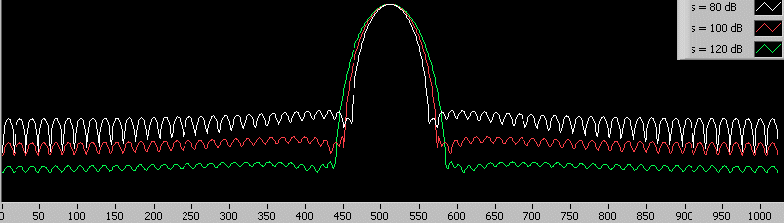
\includegraphics[scale=0.65]{CDSW_3}}
  \hfill
\end{figure}
\subsection{Force Window}
\begin{equation}
w(n) = \begin{cases} 1 & 0 \leq n \leq d \\ 0 & Otherwise \end{cases}
\end{equation}
\noindent Where $d = \frac{1}{100}N\cdot (Duty Cycle)$, where the duty cycle is the percentage of time the original signal remains high versus low over one period. This can be used to analyze transients.
\section{Partial-Wave Resonances and the Ripple Structure in the Mie Normalized Extinction Cross Section - Chylek}
\subsection{Abstract}
\noindent Resonances in partial waves $a_{n}$ and $b_{n}$ are directly responsible for a ripple structure in the normalized extinction cross section. The distance $\Delta x$ in the size parameter between two neighboring resonances is equal to a basic period of a ripple structure. 
\subsection{Main Article}
\begin{wrapfigure}{l}{0.35\textwidth}
	\centering
	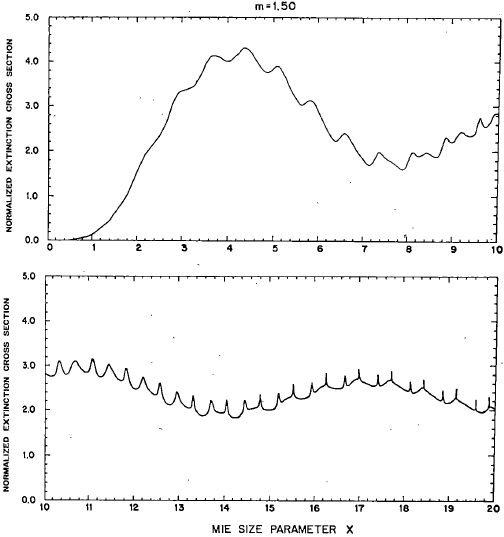
\includegraphics[width = 0.35\textwidth]{CHYLEK_1}
\end{wrapfigure}
\noindent The normalized extinction cross section for light scattering on spherical particles contains ripple structures superimposed on the main oscillation of the extinction curve. It was proposed by Van de Hulst that this is caused by interference between forward diffracted waves and surfaces waves. The Mie Partial-Wave expansion of the normalized extinction curve is:
\begin{equation}
Q_{ext}(x,m) = \frac{2}{x^2}\sum_{n=1}^{\infty} (2n+1)\Re(a_n+b_n)
\end{equation}
\noindent Where $x = \frac{2\pi r}{\lambda}$, is the radius of the particle, $a_n$ and $b_n$ are the Mie Scattering Functions, and $m$ is an index of refraction. The real parts of $a_n$ and $b_n$ are always positive, and thus the ripple structure cannot be a result of interference among partial waves $a_n$ and $b_n$. Thus, sharp narrow peaks in the ripple structure at some value $x$ can only be produced by sharp narrow peaks in the real parts of the scattering functions $a_{n}(x,m), b_{n}(x,m)$. Such peaks are called resonances. These are analogous to Van de Hulst's surface waves. Energy conversation creates the bound $0 \leq a_{n}(x,m), b_{n}(x,m) \leq 1$, where equality holds only for real indices of refraction. First consider scattering on non-absorbing spheres (m is real). Resonances can occur at such values of $x$ and $n$ for which $x \sim n$, and $\Re(a_{n}(x,m)) = 1$ or $\Re(b_{n}(x,m)) = 1$. For a given $m$ and $n$< there exists an infinite set $x_1< x_2 <x_3 <\hdots$ which satisfies this criterion. However, only the smallest size parameter $x$ which is a solution to this represents a sharp peak. The secondary peaks contribute to a smoothly varying background. There is no unambiguous way to say what is and what isn't a resonance. For large $n$, more than one peak in a given $a_{n}(x)$ or $b_{n}(x)$ function can be considered a resonance. The distance $\Delta x$ between two resonances $b_{n+1}$ and $b_{n}$ determines the basic period of the ripple structure. Suppose $b_n$ occurs at $x$ and $b_{n+1}$ occurs at $x+\Delta x$. Under this assumption, $x\gg 1$, $x\sim n$, and $mx\sim n$. For $mx>n$, we have
\begin{equation}
\Delta x =\frac{\tan^{-1}(\sqrt{m^2-1})}{\sqrt{m^2-1}}
\end{equation}
\noindent If these approximations are valid, $\Delta x$ is almost independent of $x$, for large values of $x$ and $n$, and is only dependent on $m$. $\Delta x$ is thus the basic period of a ripple structure. $\Delta x$ for $a_{n}$ is also given by this equation for large $n$ and $x$, and $mx>n$. This explains the double peak feature found inside a basic period $\Delta x$. For complex indices of refraction, the position of the resonances remain the same, however the height of the resonance peak changes causing the magnitudes of the peaks of the ripple structure to also change. The resonance peaks are changed considerably more than the broader secondary peaks contributing to the background. This supports the hypothesis that the partial-wave resonances are connected with photons traveling along a surface of a sphere, and consequently being altered absorption. 
\section{Hanning Function - Wolfram Article}
An apodization function, also called the Hann function, is frequently used to reduce leakage in discrete Fourier Transforms. The Hanning Function is given by:
\begin{equation}
A(x) = \cos^{2}(\frac{\pi x}{2a}) = \frac{1}{2}\big(1+\cos(\frac{\pi x}{a})\big)
\end{equation}
\noindent Where $a$ is its FWHM. The instrument function is:
\begin{equation}
I(k) = \frac{a\sinc(2\pi k a)}{1-4a^2 k^2} = a\big(\sinc(2\pi k a)+ \frac{1}{2}\sinc(2\pi k a-\pi)+\frac{1}{2}\sinc(2\pi k a + \pi)\big)
\end{equation}
\noindent Let $u = 2\pi k a$. Then $I(u) = a\frac{\sinc(u)}{1-\frac{u^2}{\pi^2}}$. The half-max occurs at $u_{\frac{1}{2}} = 2\pi k_{\frac{1}{2}}a = \pi$. For $L = 2a$, the FWHM is $FWHM = 2k_{\frac{1}{2}} = \frac{1}{a} = \frac{2}{L}$. The extrema satisfies $\frac{dA}{du} = \frac{\pi^2(-u^3\cos(u)+3u^2\sin(u)+\pi^2\cos(u)-\pi^2\sin(u))}{u^2(\pi^2-u^2)^2} = 0$. The first two roots are $u=7.42024$ and $10.7061$, corresponding to the first side lobe minimum and maximum, respectively. 
\section{Hamming Function - Wolfram Article}
\noindent In mathematica, for $L\in \mathbb{N}$, $w = hamming(L)$ returns an $L-$point symmetric Hamming window in the column vector $w$. The coefficients of a Hamming window are computed from the following equation:
\begin{equation}
w(n) = 0.54-0.56\cos(2\pi \frac{n}{N}), 0\leq n \leq L-1
\end{equation}
\noindent $w=hamming(L,'sflag')$ returns an $L-$point Hamming window using the window sampling specified by $'sflag'$. 'Symmetric' is the default. 'Perioid' is useful for DFT/FFT purposes, such as in spectral analysis. DFT/FFT contains an implicit periodic extension and the periodic flag enables a signal windowed with a periodic window to have perfect periodic extension. When 'periodic' is specified, hamming computes a length $L+1$ window and returns the first $L$ points. 
\section{Understanding FFTs and Windowing}
The goal of this article is learn about the time and frequency domains, fast Fourier transforms, and windowing. The Fourier transform takes a signal and breaks it down into sine waves of different amplitudes and frequencies. Real-world signals are usually viewed as a voltage changing over time. This is referred to as the time domain. Fourier's theorem states that any piecewise differentiable function (i.e. a sufficiently smooth function) that is periodic on some interval may be represented by the weighted sum of sines. For example, a square wave may be written as $\sum_{k=0}^{\infty}\frac{\sin(\pi x(2k+1))}{2k+1}$. This will converge to a square wave for all $x$, with the exception of the integers. This is the Gibbs phenomenon. If you are given a signal, you can deconstruct the signal into sines and then analyze the different frequencies present in the original signal. The Fourier transform deconstructs a time domain representation of a signal into a the frequency domain representation. The frequency domain shows the voltages present at varying frequencies. A digitizer samples a waveform and transforms it into discrete values. A Discrete Fourier Transform (DFT) is needed here. A Fast Fourier Transform (FFT) is an optimized implementation of a DST. The Fourier Transform of a sine wave is a spike at the frequency of the sine wave. The Fourier Transform of a sum of sine waves is a sequence of spikes at the frequencies of the corresponding to these waves, weighted by the amplitude of the waves. The frequency domain can be used to show how clean a signal actually is. For example, suppose you have a sine wave in the time domain, such as the image to the left. While it looks like a nice sine wave, when one examines the frequency domain of the signal we see that it is actually the sum of two sine waves, one being the main signal and the other being noise. The frequency domain is great for showing how clean a signal is and where the noise is. There are limitations to FFTs and the signal clarity can be improve with windowing. FFTs measure the frequency component of a signal based on a finite set of data. Both the time and frequency domains are circular topologies, so the two endpoints of the time waveform are interpreted as though they were connected together. When the measured signal is periodic and an integer number of periods fill the acquisition time interval, the FFT looks fine. Many times the measured signal isn't an integer number of periods. The finiteness of the measured signal may result in a truncated waveform with different characteristics from the original continuous-time signal, and the finiteness can introduce sharp transition changed into the measured signal. These sharp transitions are discontinuities. These discontinuities show up in the frequency domain as high frequency components not present in the actual signal. These frequencies can be higher than the Nyquist frequency and are aliased between $0$ and half of your sampling rate. The spectrum you get is thus a smeared version. It appears as if energy at one frequency leaks into other frequencies. This is called spectral leakage. These effects can be minimized by windowing. Windowing reduces the amplitude of the discontinuities at the boundaries of each finite sequence acquired by the digitizer. Windowing consists of multiplying the time record by a finite-length window with an amplitude that gradually and smoothly decays to zero at the edges. This makes the waveforms meet an results in a continuous waveform without sharp transitions. There are several types of windows. The frequency characteristic of a window is a continuous spectrum with a main lobe and several side lobes. The main lobe is centered at each frequency component of the time-domain signal, and the side lobes approach zero. The height of the side lobes indicates the affect the windowing function has on frequencies around the main lobes. The side lobe from a strong sinusoidal signal can overpower the main lobe of a nearby weak sinusoidal signal. Typically, lower side lobes reduce leakage in the measured FFT but increase the bandwidth of the major lobe. The side lobe roll-off rate is the asymptotic decay rate of the side lobe peaks. By increasing this, the spectral leakage can be reduced.
\begin{enumerate}
\item If the signal contains strong interfering frequency components distant from the frequency of interest, choose a smoothing windowing with a high side lobe roll-off rate
\item If the signal contains strong interfering signals near the frequency of interest, choose a window function with a low maximum side lobe level.
\item If the frequency of interest contains two or more signals very near to each other, spectral resolution is important. Choose a smoothing window with a very narrow main lobe.
\item If the amplitude accuracy of a single frequency component is more important than the exact location of the component in a given frequency bin, choose a window with a wide main lobe.
\item The Hanning (Hann) window is satisfactory in $95\%$ of cases. It has good frequency resolution and reduced spectral leakage. 
\end{enumerate}
Using no window is often called the uniform or rectangular window. The Hamming and Hanning windows have a sinusoidal shape. The Hanning window tends to zero at the edge of the window, the Hamming window does not. The Hamming window is better at cancelling the nearest lobe but poorer at cancelling others. The Blackman-Harris window results in a wide peak, but good side lobe compression. A Kaiser-Bessel window strikes a balance among the various conflicting goals of amplitude accuracy, side lobe distance, and side lobe height. This window often reveals signals close to the noise floor. There are many other windows that can be used, and a table of them and when they are useful is given on the left. There is no true universal window and different windows cater to different features.
\section{Low-Complexity Real-Time Single-Tone Phase and Frequency Estimation}
Distributed transmit beamforming is a technique in which two or more signle-antenna transmitters simultaneously transmit with phase-aligned carriers such that the passband signals coherently combine at an intended destination. The transmitters form a virtual antenna array and can achieve all of the gains of a conventional antenna array. This requires a precise carrier synchronization among the transmitters with timing errors significantly smaller than a carrier period. Several carrier synchronization techniques have been proposed to facilitate distributed transmit beamforming. A common feature is that the nodes participating in the beamformer must be able to accurately and quickly estimate the phase and frequency of one or more sinusoidal beacons received from other nodes in the network. We consider a signal model with a received signal given as:
\begin{equation}
z(t) = be^{i(\omega t+\theta)}+w(t)
\end{equation}
Where $b,\omega,$ and $\theta$ denote the unknown amplitude, frequency, and phase of the signal, respectively, and $w(t)$ denotes zero-mean proper complex additive white Gaussian noise. The received signal is sampled at a constant rate $f_{s} = \frac{1}{T}$. This produces a discrete time observation of $N$ samples:
\begin{equation}
z[n] = z(t_{0}+nT) = be^{i(\omega(t_{0}+nT)+\theta)}+\eta[n]
\end{equation}
For $n=0,1,\hdots, N-1$, where $t_0$ denotes the time of the first sample, and $\eta[n]$ is a zero-mean proper complex Gaussian random variable with $\textrm{Var}\{\Re(\eta[k])\} = \textrm{Var}\{\Im(\eta[k])\} =\sigma^2$ and $\textrm{cov}\{\Re(\eta[k]),\Im(\eta[k])\} = 0$. It is assumed that $\eta[n]$ are independent and identically distributed for $n=0,\hdots, N-1$. This observation is provided as an input to a phase and frequency estimator. The phase and frequency estimates generated are denoted $\hat{\theta}$ and $\hat{\omega}$, respectively. The errors are $\overline{\theta} = \theta - \hat{\theta}$ and $\overline{\omega} = \omega - \hat{\omega}$. Given a joint density of the observation, the maximum likelihood estimator seeks to find the value of the unknown parameters that maximizes the likelihood equation $\hat{\lambda} = \arg \underset{\lambda \in \Lambda}\arg \log\big(P_{Z}(z;\lambda)\big)$, where $p_{Z}(z;\lambda)$ is the joint density of the observation parameterized by $\lambda$. When the observations are independent and identically distributed Gaussians, the maximum likelyhood estimator possesses three desirable asymptotic properties as the number of samples in the observation becomes large: Asymptotic unbiasedness, asymptotic efficiency, and asymptotically Gaussian estimation errors. The maximum likelihood frequency estimate can be computed as $\hat{\omega} = \arg\underset{\omega}\max|A(\omega)|$, where $A(\omega) = \frac{1}{N}\sum_{n=0}^{N-1}z[n]e^{-in\omega T}$. The maximum likelihood phase estimate is $\hat{\theta} = \textrm{angle}\{e^{-i\hat{\omega}t_{0}}A(\hat{\omega})\}$. Given that the M-point DFT is a sampled version of $A(\omega)$ at frequencies $\omega = \frac{2\pi k}{MT}$, $k=0,\hdots, M-1$, a common approach to maximum likelihood frequency estimation is to use an FFT to compute $A(\frac{2\pi k}{MT})$ for $k=0,\hdots, M-1$, and then compute $\hat{\omega} = \arg\underset{\omega \in \Omega}\max |A(\omega)|$, where $\Omega = \{0,\frac{2\pi}{MT},\hdots, \frac{2\pi(M-1)}{MT}\}$. There is then a tradeoff between estimation accuracy and computational complexity. The achievable accuracy depends on the frequency resolution of the $M-$point FFT. That is, on $\frac{f_{s}}{M}$. In low SNR scenarios, where $\frac{b}{2\sigma^2}$ is small, fine frequency resolution is not necessary because of the noise. In high SNR scenarios, the maximum likelihood estimation may be limited by the frequency resolution. An additional difficulty of applying the FFT based maximum likelihood estimation to carrier synchronization in distributed transmit beamforming systems is that the FFT requires the entire observation to be present to begin processing. A high resolution FFT may incur significant processing delay after the conclusion of the observation. Phase locked loops (PLLS) are used for synchronizing a local oscillator to an external reference signal. They can be used to efficiently extract the phase and frequency from an observation of a single-tone signal in noise. The PLL is composed of three elements: A phase detector, a loop filter, and a voltage controlled oscillator. In the absence of noise, the quadrature phase detector output is $v[n] = K_{d}b\sin(\Delta[n])$< where $K_{d}$ is the phase detector gain parameter, $\Delta[n]$ is the phase difference between the input and feedback signals. The loop filter serves to suppress noise at the output of the phase detector. The output of the loop filter $u[n]$ is connected to the VCO which generates a complex exponential input $y[n]$ for feedback to the phase detector at frequency $\omega_{o}[n] = \omega_{nom}+K_{o}u[n]$, where $\omega_{nom}$ is the nominal frequency of the VCO in the absence of a control input and $K_{o}$ is the VCO gain parameter. The VCO phase is then updated $\phi_{o}[n+1] = \phi_{o}[n]+T\omega_{o}[n]$. The feedback $y[n] = e^{-i\phi_{o}[n+1]}$ is then computed and fed back to the phase detector to be multiplied with the next input sample. Given an $N-$sample observation a frequency estimate can be made $\hat{\omega} = \omega_{o}[N-1] = \omega_{nom}+K_{o}[N-1]$. The phase estimate is then $\hat{\theta}=\phi_{o}[N-1]-(N-1)T\hat{\omega}$. The PLL phase estimate is computed by subtracting the estimated accumulated phase over the observation from the final phase of the VCO. When the PLL is locked and $\Delta[n]$ is small such that $\sin(\Delta[n]) \approx \Delta[n]$, the PLL can be analyzed as a linear system. The discrete time transfer function relating the PLL output phase and input phase is then:
\begin{equation}
H_{\phi}(z) = \frac{\Phi_{o}(z)}{\Phi_{in}(z)} = \frac{bK_{d}K_{o}F(z)L(z)}{1+bK_{d}K_{o}F(z)L(z)}
\end{equation}
Where $L(z) = \frac{Tz^{-1}}{1-z^{-1}}$ and $F(z)$ is the discrete-time transfer function of the loop filter. The discrete-time transfer function relating the PLL output frequency and input phase is:
\begin{equation}
H_{\omega}(z) = \frac{\Omega_{o}(z)}{\Phi_{in}(z)} = \frac{bK_{d}K_{o}F(z)}{1+bK_{d}K_{o}F(z)L(z)}
\end{equation}
Zero-crossing phase and frequency estimation is based on the observation that the phase of the signal is a first-order polynomial in $t$. That is, $\phi(t) = \omega(t)+\theta$. The slope and intercept of this line correspond to the frequency and phase of the observed signal. If $L\geq 2$ points on this line can be measured, then the slope and intercept of the line can be determined exactly. In the presence of noise, linear regression can be used. The zero-crossing phase and frequency estimator generates the set $\{(t_1,\phi_1),\hdots, (t_{L},\phi_{L})\}$ by detecting zero crossing in the real and imaginary components of the signal. We let $S_{R}$ be the set of real zero-crossings, and $S_{I}(\ell)$ the imaginary set, where $\ell$ is an integer parameter to facilitate alignment with the coordinate set obtained from the real part. Letting $S(\ell) = S_{R}\cup S_{I}$, we perform linear regression on this set to determine the slope and intercept of the phase line. The total squared error is:
\begin{equation}
\mathcal{E}(\ell) = \sum_{n=0}^{N-1} \bigg|be^{i\big(\hat{\omega}(\ell)nT+\hat{\theta}(\ell)\big)}-z[n]\bigg|^2
\end{equation}
The zero-crossing phase and frequency estimator can be implemented on a sample-by-sample basis. 
\section{One-Dimensional Phase Unwrapping Problem}
\section{Rev 280 Occultation}
\section{Rev 282 Occultation}
\chapter{Notes on Mathematics}
\section{Atmospheric Occultation}
\subsection{Titan Geometry}
\begin{figure}[H]
	\centering
	\begin{subfigure}[b]{0.49\textwidth}
	    \centering
        \resizebox{\textwidth}{!}{
        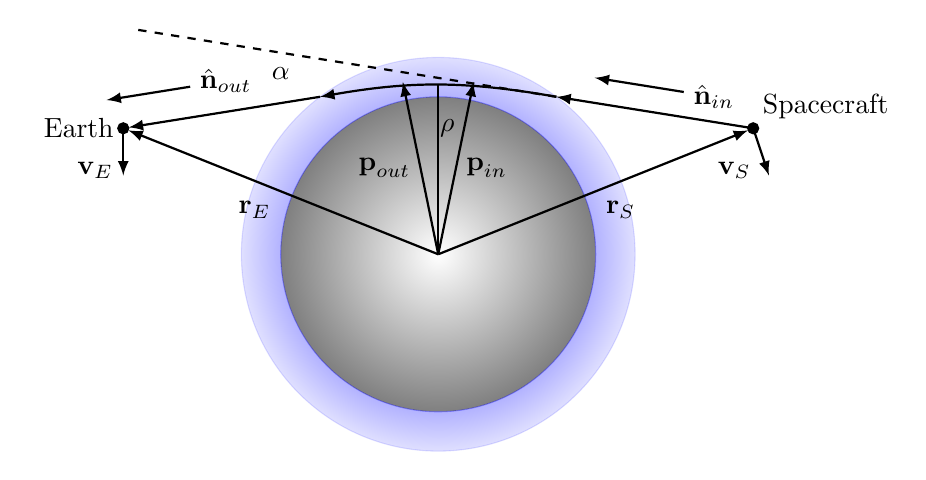
\begin{tikzpicture}[axis/.style={very thick, ->, >=stealth'},
            important line/.style={thick},
            dashed line/.style={dashed, thin},
            pile/.style={thick,->, >=stealth', shorten <=2pt,shorten>=2pt},every node/.style={color=black}]
            \coordinate (S)  at (4,1.6);
            \coordinate (E)  at (-4,1.6);
            \coordinate (O)  at (0,0);
            \coordinate (p1) at (-1.5,2);
            \coordinate (p2) at (1.5,2);
            \coordinate (P) at (0,2.2);
            \shade [even odd rule,inner color=white,outer color=gray] (0, 0) circle (2cm);
            \filldraw[even odd rule,blue ,path fading=ringo] (0,0) circle (25mm) (0,0) circle (2cm);
            \filldraw[black] (E) circle (2pt) node[left] {Earth};
            \filldraw[black] (S) circle (2pt) node[above right] {Spacecraft};
        \begin{scope}[>={latex[black]},every edge/.style={draw=black,thick}]
            \path [->] (S) edge (p2);
            \path [->] (p2) edge[bend right=10] (p1);
            \path [->,shorten >=2pt,shorten <=0cm,->] (p1) edge (E);
            \path [->] (O) edge node[right] {$\textbf{p}_{in}$} (0.45,2.18874);
            \path [->] (O) edge node[left] {$\textbf{p}_{out}$} (-0.45,2.18874);
            \path [->,shorten >=2pt,shorten <=0cm,->] (O) edge node[below left] {$\mathbf{r}_{E}$} (E);
            \path [->,shorten >=2pt,shorten <=0cm,->] (O) edge node[below right] {$\mathbf{r}_{S}$} (S);
            \path [->] (S) edge node[below left] {$\mathbf{v}_{S}$} (4.2,1);
            \path [->] (E) edge node[below left] {$\mathbf{v}_{E}$} (-4,1);
            \path (O) edge (0,2.15);
        \end{scope}
            \node (nin) at (3.5,2) {$\hat{\mathbf{n}}_{in}$};
            \node (nout) at (-2.7,2.2) {$\hat{\mathbf{n}}_{out}$};
            \draw[>={latex[black]},thick,shorten >=1cm,shorten <=0cm,->] (nin) -- +($(p2)-(S)$);
            \draw[>={latex[black]},thick,shorten >=1cm,shorten <=0cm,->] (nout) -- +($(E)-(p1)$);
            \draw[thick,dashed] (p2) -- ($(S)!8cm!(p2)$);
            \node at (-2,2.3) {$\alpha$};
            \node at (-0.1,1.6) [right] {$\rho$};
        \end{tikzpicture}}
    	\caption{Geometry of an Occultation of Titan}
	    \label{fig:math_titan_geom_vec}
    \end{subfigure}
    \begin{subfigure}[b]{0.49\textwidth}
        \centering
        \resizebox{\textwidth}{!}{
        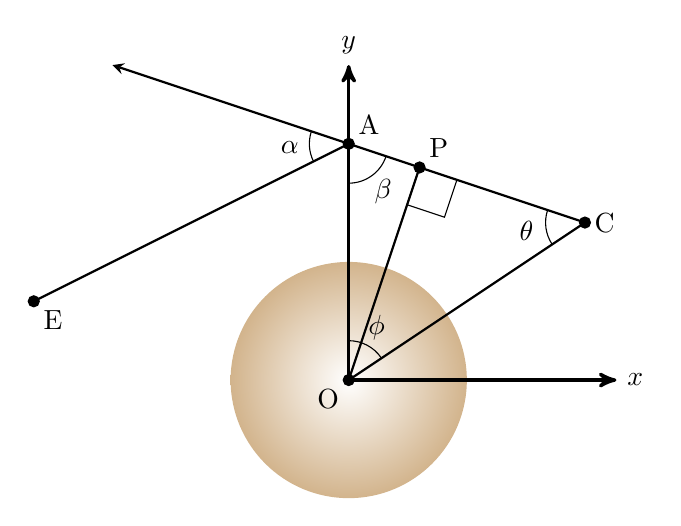
\begin{tikzpicture}[axis/.style={very thick, ->, >=stealth'},important line/.style={thick},
        dashed line/.style={dashed, thin},pile/.style={thick,->, >=stealth', shorten <=2pt,shorten>=2pt},every node/.style={color=black}]
        \coordinate (O) at (0,0) {};
        \coordinate (E) at (-4,1) {};
        \coordinate (C) at (3,2) {};
        \coordinate (A) at (0,3) {};
        \coordinate (P) at (0.9,2.7) {};
        \coordinate (Space) at (-3,4) {};
        \shade[inner color=white,outer color=Tan] (0,0) circle (1.5);
        \draw[axis] (0,0) -> (0,4)node(yline)[above] {$y$};
        \draw[axis] (0,0) -> (3.4,0)node(xline)[right] {$x$};
        \draw[thick] (0,0) -- (3,2);
        \filldraw[black] (3,2) circle (2pt) node[right] {C};
        \filldraw[black] (0,0) circle (2pt) node[below left] {O};
        \draw[thick, ->,>=stealth] (3,2) -- (-3,4);
        \filldraw[black] (0,3) circle (2pt) node[above right] {A};
        \draw[thick] (0,3) -- (-4,1);
        \filldraw[black] (-4,1) circle (2pt) node[below right] {E};
        \pic [draw=black, -, "$\alpha$", angle eccentricity=1.5] {angle = Space--A--E};
        \pic [draw=black, -, "$\beta$", angle eccentricity=1.5] {angle = O--A--C};
        \pic [draw=black, -, "$\theta$", angle eccentricity=1.5] {angle = A--C--O};
        \pic [draw=black, -, "$\phi$", angle eccentricity=1.5] {angle = C--O--A};
        \draw[thick] (0,0) -- (0.9,2.7);
        \filldraw[black] (0.9,2.7) circle (2pt) node[above right] {P};
        \tkzMarkRightAngle[draw=black,size=0.5](O,P,C);
    \end{tikzpicture}}
    \caption{Geometry of the Bending Angle}
    \label{fig:math_geo_bending_angle}
    \end{subfigure}
\end{figure}
The following definitions are used:
\begin{enumerate}[itemsep=0pt]
    \begin{multicols}{2}
        \item $O$ is Titan.
        \item $E$ is Earth.
        \item $C$ is Cassini.
        \item $\mathbf{r}_{E} = \overrightarrow{OE}$
        \item $\mathbf{v}_{E} = \frac{d}{dt}\mathbf{r}_{E}$
        \item $\mathbf{r}_{S} = \overrightarrow{OC}$
        \item $\mathbf{v}_{S} = \frac{d}{dt}\mathbf{r}_{S}$
        \item $\mathbf{p}_{in}$ is the projection of $O$ onto $\overline{AC}$
        \item $\mathbf{p}_{out}$ is the projection of $O$ onto $\overline{EA}$
        \item $\alpha$ is the bending angle ($\pi-\angle EAC$)
        \item $\hat{\mathbf{n}}_{in}$ is the direction of the emission.
        \item $\hat{\mathbf{n}}_{out}$ is the direction of the reception.
        \item The ray plane is the plane $OEC$
        \item $\phi = \angle OAC$
        \item $\theta = \angle ACO$
        \item $\beta = \angle AOC$
    \end{multicols}
    \vspace{-3ex}
    \item $A$ is the intersection of the lines starting at $C$ and $E$, parallel to $\hat{\mathbf{n}}_{in}$ and $\hat{\mathbf{n}}_{out}$, respectively.
\end{enumerate}
The following assumptions are made:
\begin{enumerate}
    \begin{multicols}{2}
        \item $\angle OAE = \angle OAC$
        \item $A$ lies in the plane $OEC$
    \end{multicols}
\end{enumerate}
\begin{theorem}
\label{theorem:ray_plane_perp_to_r_e_cross_r_s}
The ray plane is perpendicular to $\hat{\mathbf{z}} = \frac{\mathbf{r}_{S}\times \mathbf{r}_{E}}{\norm{\mathbf{r}_{S}\times \mathbf{r}_{E}}}$
\end{theorem}
\begin{proof}
As the ray plane is the plane $OEC$, $\mathbf{r}_{S}$ and $\mathbf{r}_{E}$ lie parallel to this plane. Moreover, during an occultation, $\mathbf{r}_{S}$ and $\mathbf{r}_{E}$ are not parallel and therefore $OEC$ is uniquely determined by $\mathbf{r}_{E}$, $\mathbf{r}_{S}$, and the point $O$. But $\hat{\mathbf{z}} = \frac{\mathbf{r}_{S}\times \mathbf{r}_{E}}{\norm{\mathbf{r}_{S}\times \mathbf{r}_{E}}}$ is perpendicular to both $\mathbf{r}_{E}$ and $\mathbf{r}_{S}$. Therefore $\hat{\mathbf{z}}$ is perpendicular to the ray plane.
\end{proof}
\begin{theorem}
\label{theorem:r_e_dot_p_out_equal_p_out_square}
$\mathbf{r}_{E}\cdot \mathbf{p}_{out} = \norm{\mathbf{p}_{out}}^2$
\end{theorem}
\begin{proof}
$\mathbf{p}_{out}$ is the projection of the $O$ onto $\overline{EA}$. But $\overline{EA}$ lies parallel to $\hat{\mathbf{n}}_{out}$, and therefore $\mathbf{p}_{out}$ and $\hat{\mathbf{n}}_{out}$ are orthogonal, and thus $\mathbf{p}_{out}\cdot\hat{\mathbf{n}}_{out}=0$. Moreoever, $\mathbf{r}_{E} = \mathbf{p}_{out}+(\mathbf{r}_{E}\cdot \hat{\mathbf{n}}_{out}) \hat{\mathbf{n}}_{out}$. But then:
\begin{align*}
    \mathbf{p}_{out}\cdot \mathbf{r}_{E} &= \mathbf{p}_{out}\cdot\big(\mathbf{p}_{out}+(\mathbf{r}_{E}\cdot \hat{\mathbf{n}}_{out})\hat{\mathbf{n}}_{out}\big)\\
    \Rightarrow \mathbf{p}_{out}\cdot \mathbf{r}_{E} &= \mathbf{p}_{out}\cdot \mathbf{p}_{out} + (\mathbf{r}_{E}\cdot \hat{\mathbf{n}}_{out}) \mathbf{p}_{out}\cdot \hat{\mathbf{n}}_{out}\\
    \Rightarrow \mathbf{p}_{out}\cdot \mathbf{r}_{E} &= \mathbf{p}_{out}\cdot \mathbf{p}_{out}
\end{align*}
Therefore $\mathbf{p}_{out}\cdot \mathbf{r}_{E} = \norm{\mathbf{p}_{out}}^2$
\end{proof}
\begin{theorem}
$\alpha = \cos^{-1}(\hat{\mathbf{n}}_{in}\cdot \hat{\mathbf{n}}_{out})$
\end{theorem}
\begin{proof}
By definition, $\alpha = \pi - \angle EAC$. But $\hat{\mathbf{n}}_{out}$ lies parallel to $\overrightarrow{AE}$, and $-\hat{\mathbf{n}}_{in}$ lies parallel to $\overrightarrow{AC}$. Therefore:
\begin{equation*}
-\hat{\mathbf{n}}_{out}\cdot \hat{\mathbf{n}}_{in} = \hat{\mathbf{n}}_{out}\cdot (-\hat{\mathbf{n}}_{in}) = \norm{\hat{\mathbf{n}}_{out}}\norm{-\hat{\mathbf{n}}_{in}}\cos(\angle EAC)
\end{equation*}
But $\hat{\mathbf{n}}_{in}$ and $\hat{\mathbf{n}}_{out}$ are unit vectors, and therefore $\norm{\hat{\mathbf{n}}_{out}} = \norm{-\hat{\mathbf{n}}_{in}} = 1$. Therefore:
\begin{equation*}
    \angle EAC = \cos^{-1}(-\hat{\mathbf{n}}_{out}\cdot\hat{\mathbf{n}}_{in})
\end{equation*}
But $\alpha = \pi - \angle EAC$, and $\cos^{-1}(-x) = \pi - \cos^{-1}(x)$. Therefore:
\begin{equation*}
    \alpha = \pi - \angle EAC = \pi - \big(\pi - \cos^{-1}(\hat{\mathbf{n}}_{out}\cdot \hat{\mathbf{n}}_{in})\big) = \cos^{-1}(\hat{\mathbf{n}}_{out}\cdot \hat{\mathbf{n}}_{in})
\end{equation*}
\end{proof}
\begin{theorem}
$\theta = \cos^{-1}\big(\frac{(-\mathbf{r}_{S})\cdot \hat{\mathbf{n}}_{in}}{\norm{\mathbf{r}_{S}}}\big)$
\end{theorem}
\begin{proof}
For $\theta = \angle OCA$. But $\hat{\mathbf{n}}_{in}$ is parallel with $\overrightarrow{CA}$, and $(-\mathbf{r}_{S})$ is parallel with $\overrightarrow{CO}$. Therefore:
\begin{align*}
    (-\mathbf{r}_{S})\cdot \hat{\mathbf{n}}_{in} &= \norm{(-\mathbf{r}_{S})}\norm{\hat{\mathbf{n}}_{in}}\cos(\theta)\\
    \Rightarrow \theta &= \cos^{-1}\bigg(\frac{(-\mathbf{r}_{S})\cdot \hat{\mathbf{n}}_{in}}{\norm{\mathbf{r}_{S}}}\bigg)
\end{align*}
\end{proof}
\begin{theorem}
$\beta = \pi - \frac{1}{2}\cos^{-1}\bigg(\frac{\mathbf{r}_{s}\cdot \mathbf{r}_{E}}{\norm{\mathbf{r}_{s}}\norm{\mathbf{r}_{E}}}\bigg) - \frac{1}{2}\cos^{-1}\bigg(\frac{\mathbf{r}_{E}\cdot \hat{\mathbf{n}}_{out}}{\norm{\mathbf{r}_{E}}}\bigg) - \frac{1}{2}\cos^{-1}\bigg(\frac{(-\mathbf{r}_{s})\cdot \hat{\mathbf{n}}_{in}}{\norm{\mathbf{r}_{s}}}\bigg)$
\end{theorem}
\begin{proof}
The sum of the angles in $OEAC$ is $2\pi$. But $\angle OAE = \angle OAC = \phi$, and therefore:
\begin{align*}
    2\beta &=\angle EAC \\
    \Rightarrow 2\pi &= 2\beta + \angle AEO + \angle EOC + \angle OCA\\
    \Rightarrow \beta &= \pi - \frac{\angle AEO}{2}-\frac{\angle EOC}{2}-\frac{\angle OCA}{2}
\end{align*}
But:
\begin{align*}
(-\hat{\mathbf{n}}_{out})\cdot (-\hat{\mathbf{r}}_{E}) &= \norm{\mathbf{r}_{E}}\cos(\angle AEO)\\
\Rightarrow \angle AEO &= \cos^{-1}\bigg(\frac{\hat{\mathbf{n}}_{out}\cdot \mathbf{r}_{E}}{\norm{\mathbf{r}_{E}}}\bigg)
\end{align*}
Also:
\begin{align*}
    \mathbf{r}_{E}\cdot \mathbf{r}_{S} &= \norm{\mathbf{r}_{E}}\norm{\mathbf{r}_{S}}\cos(\angle EOC)\\
    \Rightarrow \angle EOC &= \cos^{-1}\bigg(\frac{\mathbf{r}_{E}\cdot \mathbf{r}_{S}}{\norm{\mathbf{r}_{E}}\norm{\mathbf{r}_{S}}}\bigg)
\end{align*}
But $\angle OCA = \theta = \cos^{-1}\big(\frac{(-\mathbf{r}_{S})\cdot \hat{\mathbf{n}}_{in}}{\norm{\mathbf{r}_{S}}}\big)$. Therefore:
\begin{equation*}
\beta = \pi - \frac{1}{2}\cos^{-1}\bigg(\frac{\mathbf{r}_{s}\cdot \mathbf{r}_{E}}{\norm{\mathbf{r}_{s}}\norm{\mathbf{r}_{E}}}\bigg) - \frac{1}{2}\cos^{-1}\bigg(\frac{\mathbf{r}_{E}\cdot \hat{\mathbf{n}}_{out}}{\norm{\mathbf{r}_{E}}}\bigg) - \frac{1}{2}\cos^{-1}\bigg(\frac{(-\mathbf{r}_{s})\cdot \hat{\mathbf{n}}_{in}}{\norm{\mathbf{r}_{s}}}\bigg)
\end{equation*}
\end{proof}
\begin{theorem}
$\alpha = \pi - 2\beta$
\end{theorem}
\begin{proof}
$\alpha$ and $\angle EAC$ are supplementary to the ray $\overrightarrow{CA}$, and therefore $\alpha + \angle EAC = \pi$. But $\angle EAC = \angle EAC + \angle OAC = 2\beta$. Therefore $\alpha + 2\beta = \pi$. Thus, $\alpha = \pi - 2\beta$.
\end{proof}
\begin{theorem}
$\theta = \frac{\pi}{2}+ \frac{\alpha}{2}-\phi$
\end{theorem}
\begin{proof}
As the angles of a triangle sum to $\pi$, $\theta+\beta+\phi = \pi$. But $\alpha = \pi - 2\beta \Rightarrow \beta = \frac{\pi}{2}-\frac{\alpha}{2}$. So we have:
\begin{align*}
    \theta+\phi+\beta &=\pi \\
    \Rightarrow \theta+\phi+\frac{\pi}{2}-\frac{\alpha}{2} &= \pi\\
    \Rightarrow \theta &= \frac{\pi}{2} +\frac{\alpha}{2}-\phi
\end{align*}
\end{proof}
\begin{theorem}
$\phi = \frac{1}{2}\cos^{-1}\bigg(\frac{\mathbf{r}_{s}\cdot \mathbf{r}_{E}}{\norm{\mathbf{r}_{s}}\norm{\mathbf{r}_{E}}}\bigg) + \frac{1}{2}\cos^{-1}\bigg(\frac{\mathbf{r}_{E}\cdot \hat{\mathbf{n}}_{out}}{\norm{\mathbf{r}_{E}}}\bigg) - \frac{1}{2}\cos^{-1}\bigg(\frac{(-\mathbf{r}_{s})\cdot \hat{\mathbf{n}}_{in}}{\norm{\mathbf{r}_{s}}}\bigg) $
\end{theorem}
\begin{proof}
For:
\begin{align*}
    \pi &=\beta+\theta+\phi\\
    \theta &= \cos^{-1}\big(\frac{(-\mathbf{r}_{S})\cdot\hat{\mathbf{n}}_{in}}{\norm{\mathbf{r}_{S}}}\big)\\
    \beta &= \pi-\frac{1}{2}\cos^{-1}\bigg(\frac{\mathbf{r}_{s}\cdot \mathbf{r}_{E}}{\norm{\mathbf{r}_{s}}\norm{\mathbf{r}_{E}}}\bigg) - \frac{1}{2}\cos^{-1}\bigg(\frac{\mathbf{r}_{E}\cdot \hat{\mathbf{n}}_{out}}{\norm{\mathbf{r}_{E}}}\bigg) - \frac{1}{2}\cos^{-1}\bigg(\frac{(-\mathbf{r}_{s})\cdot \hat{\mathbf{n}}_{in}}{\norm{\mathbf{r}_{s}}}\bigg)\\
    \Rightarrow \phi & = \frac{1}{2}\cos^{-1}\bigg(\frac{\mathbf{r}_{s}\cdot \mathbf{r}_{E}}{\norm{\mathbf{r}_{s}}\norm{\mathbf{r}_{E}}}\bigg) + \frac{1}{2}\cos^{-1}\bigg(\frac{\mathbf{r}_{E}\cdot \hat{\mathbf{n}}_{out}}{\norm{\mathbf{r}_{E}}}\bigg) - \frac{1}{2}\cos^{-1}\bigg(\frac{(-\mathbf{r}_{s})\cdot \hat{\mathbf{n}}_{in}}{\norm{\mathbf{r}_{s}}}\bigg)
\end{align*}
\end{proof}
\begin{theorem}
\label{theorem:impact_parameter_p_closed_form_solution}
$p = \norm{\mathbf{p}_{in}} = \norm{\mathbf{r}_{S}}\cos(\phi - \frac{\alpha}{2})$
\end{theorem}
\begin{proof}
As $P$ is the orthogonal projection of $O$ onto $\overline{CA}$, $\angle OPC = \frac{\pi}{2}$. But then:
\begin{equation*}
    |\overline{OP}| = |\overline{OC}|\sin(\angle OCP)
\end{equation*}
But $|\overline{OP}| = \norm{\mathbf{p}_{in}}$, $|\overline{OC}| = \norm{\mathbf{r}_{S}}$, and $\angle OCP = \theta$. Therefore:
\begin{equation*}
    \norm{\mathbf{p}_{in}} = \norm{\mathbf{r}_{S}}\sin(\theta)
\end{equation*}
But $\theta = \frac{\pi}{2} + \frac{\alpha}{2} - \phi$, and $\sin(\frac{\pi}{2}+x) = \cos(x)$. Therefore:
\begin{equation*}
    \norm{\mathbf{p}_{in}} = \norm{\mathbf{r}_{S}}\cos\big(\frac{\alpha}{2} - \phi\big)
\end{equation*}
\end{proof}
\begin{theorem}
$\norm{\mathbf{p}_{in}} = |\overline{OA}|\sin(\beta)$
\end{theorem}
\begin{proof}
For $\overline{OP}$ is perpendicular to $\overline{CA}$, and therefore $\Delta OPA$ is a right-angled triangle, and $\overline{OA}$ is the hypotenuse. Moreoever $\angle PAO = \beta$. But then:
\begin{align*}
|\overline{OP}| &= |\overline{OA}|\sin(\angle PAO)\\
\Rightarrow |OP| &= |\overline{OA}|\sin(\beta)
\end{align*}
But $\norm{\mathbf{p}_{in}} = |\overline{OP}|$, and thus $\norm{\mathbf{p}_{in}} = |OA|\sin(\beta)$
\end{proof}
\begin{theorem}
\label{theorem:p_out_equals_p_in}
$\norm{\mathbf{p}_{in}} = \norm{\mathbf{p}_{out}}$
\end{theorem}
\begin{proof}
For $\angle OAE = \angle OAC = \beta$, and thus:
\begin{equation*}
    \norm{\mathbf{p}}_{out} = |\overline{OA}|\sin(\angle OAE) = |\overline{OA}|\sin(\beta)=\norm{\mathbf{p}}_{in}
\end{equation*}
\end{proof}
\section{Ring Occultation}
\subsection{Ring Geometry}
\begin{theorem}
\label{theorem:ring_occ_geom_x_y_z_orthonormal_basis}
If $\hat{\mathbf{u}}$ and $\hat{\mathbf{z}}$ are unit vectors and $\hat{\mathbf{u}}\times \hat{\mathbf{z}} \ne \mathbf{0}$, then $\{\big(\frac{\hat{\mathbf{u}}\times \hat{\mathbf{z}}}{\norm{\hat{\mathbf{u}}\times \hat{\mathbf{z}}}}\big)\times \hat{\mathbf{z}},\frac{\hat{\mathbf{u}}\times \hat{\mathbf{z}}}{\norm{\hat{\mathbf{u}}\times \hat{\mathbf{z}}}},\hat{\mathbf{z}}\}$ is an orthonormal basis of $\mathbb{R}^3$.
\end{theorem}
\begin{proof}
Let $\hat{\mathbf{y}} = \frac{\hat{\mathbf{u}}\times \hat{\mathbf{z}}}{\norm{\hat{\mathbf{u}}\times \hat{\mathbf{z}}}}$ and let $\hat{\mathbf{x}} = \frac{\hat{\mathbf{u}}\times \hat{\mathbf{z}}}{\norm{\hat{\mathbf{u}}\times \hat{\mathbf{z}}}}\times \hat{\mathbf{z}}$. Then $\hat{\mathbf{x}} = \hat{\mathbf{y}}\times \hat{\mathbf{z}}$. But then $\hat{\mathbf{y}}\cdot \hat{\mathbf{z}} = 0$, $\hat{\mathbf{y}}\cdot \hat{\mathbf{x}} = 0$, and $\hat{\mathbf{x}}\cdot \hat{\mathbf{z}} = 0$. Both $\hat{\mathbf{z}}$ and $\hat{\mathbf{y}}$ are unit vectors by definition, and $\hat{\mathbf{x}}$ is the cross product of two orthogonal unit vectors, and is therefore itself a unit vector. But then $\{\hat{\mathbf{x}},\hat{\mathbf{y}},\hat{\mathbf{z}}\}$ is a set of $3$ mutually orthogonal unit vectors. By the Vector Space Dimension Theorem, $\{\hat{\mathbf{x}},\hat{\mathbf{y}},\hat{\mathbf{z}}\}$ is an orthonormal basis of $\mathbb{R}^3$.
\end{proof}
\begin{definition}
The Saturnian Coordinate System is defined as a Cartesian Coordinate System where $\mathbf{u}$ is the vector from Earth to the Spacecraft, $\hat{\mathbf{z}}$ is Saturn's Pole vector, $\{\hat{\mathbf{x}},\hat{\mathbf{z}},\hat{\mathbf{z}}\} = \{\frac{\hat{\mathbf{u}}\times\hat{\mathbf{z}}}{\norm{\hat{\mathbf{u}}\times\hat{\mathbf{z}}}}\times\hat{\mathbf{z}},\frac{\hat{\mathbf{u}}\times\hat{\mathbf{z}}}{\norm{\hat{\mathbf{u}}\times\hat{\mathbf{z}}}},\hat{\mathbf{z}}\}$, and the origin is Saturn's Center.
\end{definition}
\begin{definition}
The ring plane of Saturn is the plane perpendicular to $\hat{\mathbf{z}}$ which contains the origin.
\end{definition}
\begin{theorem}
Saturn's ring plane is the $xy-$plane.
\end{theorem}
\begin{proof}
This is a restatement of the fact that $\{\hat{\mathbf{x}},\hat{\mathbf{y}},\hat{\mathbf{z}}\}$ is an orthonormal system (Theorem \ref{theorem:ring_occ_geom_x_y_z_orthonormal_basis}) and from the definition of Saturn's ring plane.
\end{proof}
\begin{theorem}
In the Saturnian Coordinate System, The Earth-Spacecraft line lies parallel to the $xz$ plane.
\end{theorem}
\begin{proof}
It suffices to show that $\hat{\mathbf{u}}$ is orthogonal to $\hat{\mathbf{y}}$. But $\hat{\mathbf{u}}\cdot \hat{\mathbf{y}} = \hat{\mathbf{u}}\cdot \frac{\hat{\mathbf{u}}\times \hat{\mathbf{z}}}{\norm{\hat{\mathbf{u}}\times \hat{\mathbf{z}}}}$, and therefore $\hat{\mathbf{u}}$ is orthogonal to $\hat{\mathbf{y}}$. Thus $\hat{\mathbf{u}} = a_1\hat{\mathbf{x}} + a_2\hat{\mathbf{z}}$, and therefore $\hat{\mathbf{u}}$ is parallel to the $xz-$plane.
\end{proof}
\begin{theorem}
In the Saturn Reference frame, Earth lies on the $xz-$plane if and only if the line from Earth to Cassini lies in it.
\end{theorem}
\begin{proof}
If $\hat{\mathbf{u}}$ lies in the $xz-$plane, then Earth must also lie in it. From the previous theorem, $\hat{\mathbf{u}}$ lies parallel to the $xz-$plane. Thus, if Earth lies in the $xz-$plane, so must $\hat{\mathbf{u}}$.
\end{proof}
\begin{theorem}
If $\hat{\mathbf{z}} = z_1\hat{\mathbf{x}}_{E}+z_2\hat{\mathbf{y}}_{E}+z_3\hat{\mathbf{z}}_{E}$ and $\mathbf{u}_{0} = u_{E_{x}}\hat{\mathbf{x}}_{E}+u_{E_{y}}\hat{\mathbf{y}}_{E}+u_{E_{z}}\hat{\mathbf{z}}_{E}$, then:
\begin{equation*}
\hat{\mathbf{y}} = y_{1}\hat{\mathbf{x}}_{E}+y_2\hat{\mathbf{y}}_{E}+y_3\hat{\mathbf{z}}_{E}
\end{equation*}
Where:
\begin{align*}
y_1 &= \frac{z_2u_{E_{z}} - z_{3}u_{E_{y}}}{\sqrt{(z_2u_{E_{z}}-z_3u_{E_{y}})^2+(z_3u_{E_{x}}-z_1u_{E_{z}})^2+(z_1u_{E_{y}}-z_2u_{E_{x}})^2}} \\
y_2 &= \frac{z_3u_{E_{x}} - z_{1}u_{E_{z}}}{\sqrt{(z_2u_{E_{z}}-z_3u_{E_{y}})^2+(z_3u_{E_{x}}-z_1u_{E_{z}})^2+(z_1u_{E_{y}}-z_2u_{E_{x}})^2}} \\
y_3 &= \frac{z_1u_{E_{y}} - z_2u_{E_{x}}}{\sqrt{(z_2u_{E_{z}}-z_3u_{E_{y}})^2+(z_3u_{E_{x}}-z_1u_{E_{z}})^2+(z_1u_{E_{y}}-z_2u_{E_{x}})^2}}
\end{align*}
\end{theorem}
\begin{proof}
$\hat{\mathbf{y}}$ is defined as $\frac{\hat{\mathbf{z}}\times \mathbf{u}_{0}}{\norm{\hat{\mathbf{z}}\times \mathbf{u}_{0}}}$. This equation is simply the computed cross-product divided by the norm.
\end{proof}
\begin{theorem}
If $\hat{\mathbf{z}} = z_1\hat{\mathbf{x}}_{E}+z_2\hat{\mathbf{y}}_{E}+z_3\hat{\mathbf{z}}_{E}$ and $\mathbf{u}_{0} = u_{E_{x}}\hat{\mathbf{x}}_{E}+u_{E_{y}}\hat{\mathbf{y}}_{E}+u_{E_{z}}\hat{\mathbf{z}}_{E}$, then:
\begin{equation*}
\hat{\mathbf{x}} = x_1 \hat{\mathbf{x}}_{E}+x_2\hat{\mathbf{y}}_{E}+x_3\hat{\mathbf{z}}_{E}
\end{equation*}
Where:
\begin{align*}
x_1 &= \frac{z_3(z_{3}u_{E_{x}}-z_1u_{E_{z}})-z_2(z_1u_{E_{y}}-z_2u_{E_{x}})}{\sqrt{(z_2u_{E_{z}}-z_3u_{E_{y}})^2+(z_3u_{E_{x}}-z_1u_{E_{z}})^2+(z_1u_{E_{y}}-z_2u_{E_{x}})^2}}\\
x_2 &= \frac{z_1(z_{1}u_{E_{y}}-z_{2}u_{E_{x}})-z_{3}(z_{2}u_{E_{z}}-z_{3}u_{E_{y}})}{\sqrt{(z_2u_{E_{z}}-z_3u_{E_{y}})^2+(z_3u_{E_{x}}-z_1u_{E_{z}})^2+(z_1u_{E_{y}}-z_2u_{E_{x}})^2}}\\
x_3 &= \frac{z_2(z_2u_{E_{z}}-z_3u_{E_{y}})-z_1(z_{3}u_{E_{x}}-z_{1}u_{E_{z}})}{\sqrt{(z_2u_{E_{z}}-z_3u_{E_{y}})^2+(z_3u_{E_{x}}-z_1u_{E_{z}})^2+(z_1u_{E_{y}}-z_2u_{E_{x}})^2}}
\end{align*}
\end{theorem}
\begin{proof}
$\hat{\mathbf{x}}$ is defined as $\hat{\mathbf{y}}\times \hat{\mathbf{z}}$. This equation is merely that product.
\end{proof}
\begin{theorem}
If $(S_x,S_y,S_z)$ is location of the center of Saturn with respect to the center of the Earth and $(x_{E},y_{E},z_{E})$ is a point in $\mathbb{R}^3$ with respect to the center of the Earth, then the change of coordinates to the Saturn-based system is:
\begin{equation*}
\begin{pmatrix} x\\y\\z \end{pmatrix} = \begin{pmatrix} x_1 & x_2 & x_3 \\ y_1 & y_2 & y_3 \\ z_1 & z_2 & z_3 \end{pmatrix} \begin{pmatrix} x_{E}-S_{x} \\ y_{E}-S_{y} \\ z_{E} - S_{z}\end{pmatrix}
\end{equation*}
\end{theorem}
\begin{proof}
The point $(x_{E}-S_{x}, y_{E}-S_{y}, z_{E}-S_{z})$ is the point $(x_{E},y_{E},z_{E})$ translated so that the center of Saturn is the new origin. The rotation matrix then aligns the Earth-based coordinates to the Saturn-based coordinates.
\end{proof}
\subsection{Derivation of Equation 4a in Marouf et al.}
Let $\hat{\mathbf{u}}$ be the unit vector pointing from Earth to Voyager. Let $\hat{\mathbf{z}}$ be the spin axis of Saturn. To make the arguments easier, we assume the line from Earth to Saturn and the line from Earth to Voyager are parallel (We assume Saturn is infinitely far away). Let $B = \sin^{-1}(\hat{\mathbf{z}}\cdot \hat{\mathbf{u}})$, and let $\hat{\mathbf{y}} = \frac{\hat{\mathbf{u}}\times \hat{\mathbf{z}}}{\norm{\hat{\mathbf{u}}\times \hat{\mathbf{z}}}}$, and $\hat{\mathbf{x}} = \hat{\mathbf{y}}\times \hat{\mathbf{z}}$. Then $\hat{\mathbf{x}}$ and $\hat{\mathbf{u}}$ are parallel. We take the origin as Saturn's center. So $\hat{\mathbf{u}} = \cos(B)\hat{\mathbf{x}}+\sin(B)\hat{\mathbf{z}}$. Let $\mathbf{r}_{0}$ be the vector pointing from Saturn to the ring intercept point, and let $\boldsymbol{\rho}$ be a vector in the ring plane. Let $\phi_0$ and $\phi$ be the angles made with $\boldsymbol{\rho}_0$ and $\boldsymbol{\rho}$ to the $x-$axis, respectively. Then $\boldsymbol{\rho}_{0} = \rho_{0}\big(\cos(\phi_0)\hat{\mathbf{x}}+\sin(\phi_{0})\hat{\mathbf{y}}\big)$ and $\boldsymbol{\rho} = \rho\big(\cos(\phi)\hat{\mathbf{x}}+\sin(\phi)\hat{\mathbf{y}}\big)$. Let $\mathbf{R}_{c}$ be the vector pointing from Saturn to Voyager. Let $D$ be the distance from the ring intercept point to Voyager. Then $\mathbf{R}_{c} = \boldsymbol{\rho}_{0}+D\hat{\mathbf{u}}$. We thus have the following:
\begin{align*}
\mathbf{R}_{c} &= \big(\rho_{0}\cos(\phi_0)+D\cos(B)\big)\hat{\mathbf{x}}+\rho_{0}\sin(\phi_{0})\hat{\mathbf{y}}+D\sin(B)\hat{\mathbf{z}}\\
\boldsymbol{\rho} &= \rho\cos(\phi)\hat{\mathbf{x}}+\rho\sin(\phi)\hat{\mathbf{y}}\\
\boldsymbol{\rho}_{0} &= \rho_{0}\cos(\phi_0)\hat{\mathbf{x}}+\rho_{0}\sin(\phi_{0})\hat{\mathbf{y}}\\
\hat{\mathbf{u}} &= \cos(B)\hat{\mathbf{x}}+\sin(B)\hat{\mathbf{z}}
\end{align*}
We wish to compute $\hat{\mathbf{u}}\cdot \boldsymbol{\rho}+\norm{\mathbf{R}_{c}-\boldsymbol{\rho}}$. We have
\begin{equation*}
\big(\cos(B)\hat{\mathbf{x}}+\sin(B)\hat{\mathbf{z}}\big)\cdot\big(\rho(\cos(\phi)\hat{\mathbf{x}}+\sin(\phi)\hat{\mathbf{y}})\big) = \rho\cos(B)\cos(\phi)
\end{equation*}
And $\norm{\mathbf{R}_{c}-\boldsymbol{\rho}} = \sqrt{(\mathbf{R}_{c}-\boldsymbol{\rho})\cdot(\mathbf{R}_{c}-\boldsymbol{\rho})}$. So we have $\sqrt{\norm{\mathbf{R}_{c}}^2+\norm{\boldsymbol{\rho}}^2-2\mathbf{R}_{c}\cdot\boldsymbol{\rho}}$. But:
\begin{align*}
\nonumber \norm{\mathbf{R}_{c}}^2 &= \rho_{0}^2\cos^2(\phi_0)+2D\rho_{0}\cos(\phi_0)\cos(B)+D^2\cos^2(B) + \rho_{0}^2\sin^2(\phi_0)+D^2\sin^2(B) \\
&= \rho_{0}^2+D^2+2D\rho_{0}\cos(\phi_0)\cos(B)
\end{align*}
And $\norm{\boldsymbol{\rho}}^2 = \rho^2$. But also:
\begin{align*}
\nonumber \mathbf{R}_{c}\cdot \boldsymbol{\rho} &= \rho\cos(\phi)\big(\rho_{0}\cos(\phi_{0})+D\cos(B)\big)+\rho\rho_{0}\sin(\phi)\sin(\phi_{0})\\
\nonumber &= \rho\rho_{0}\big(\cos(\phi)\cos(\phi_{0})+\sin(\phi)\sin(\phi_{0})\big)+\rho D\cos(B)\\
&= \rho\rho_{0}\cos(\phi-\phi_{0})+\rho D\cos(B)
\end{align*}
So we have:
\begin{align*}
\nonumber \norm{\mathbf{R}_{c}-\boldsymbol{\rho}}^2 &= \rho_{0}^2+D^2+\rho^2+2D\rho_{0}\cos(\phi_{0})\cos(B)-2\rho\rho_{0}\cos(\phi-\phi_{0})-2\rho D\cos(B)\\
&=\rho^2+\rho_{0}^2+D^2-2\rho\rho_{0}\cos(\phi-\phi_{0}) + 2D\cos(B)\big(\rho_{0}\cos(\phi_0)-\rho\cos(\phi)\big)
\end{align*}
In conclusion:
\begin{align*}
    \hat{\mathbf{u}}\cdot \boldsymbol{\rho} + \norm{\mathbf{R}_{c}-\boldsymbol{\rho}} &\phantom{+}=\phantom{+}\rho\cos(B)\cos(\phi)\\
    &\phantom{+}\phantom{=}+\sqrt{\rho^2+\rho_{0}^2 + D^2 - 2\rho\rho_{0}\cos(\phi - \phi_{0}) + 2D\cos(B)\big(\rho_{0}\cos(\phi_0) - \rho\cos(\phi)\big)}
\end{align*}
Now the definition of $\hat{T}$ is:
\begin{equation*}
\hat{T} = \frac{E_{c}}{E_{0}}e^{-ik\hat{\mathbf{u}}\cdot\mathbf{R}_{c}}
\end{equation*}
So:
\begin{equation*}
\psi = k\bigg(\norm{\mathbf{R}_{c}-\rho}^2 + \hat{\mathbf{u}}\cdot\boldsymbol{\rho} - \hat{\mathbf{u}}\cdot \mathbf{R}_{c}\bigg)    
\end{equation*}
But:
\begin{equation*}
\hat{\mathbf{u}}\cdot \mathbf{R}_{c} = \rho_{0}\cos(\phi_0)\cos(B) + D\cos^2(B) + D\sin^2(B) = \rho_{0}\cos(\phi_0)\cos(B)+D    
\end{equation*}
So we have:
\begin{align*}
\frac{\psi}{k} &=\phantom{+}\rho\cos(\phi)\cos(B) - \rho_0\cos(\phi_0)\cos(B)-D\\
&\phantom{=}+\sqrt{\rho^2+\rho_{0}^2 + D^2 - 2\rho\rho_{0}\cos(\phi - \phi_{0}) + 2D\cos(B)\big(\rho_{0}\cos(\phi_0) - \rho\cos(\phi)\big)} \\
&=\phantom{+}\cos(B)\big(\rho\cos(\phi) - \rho_{0}\cos(\phi_{0})\big) - D\\
&\phantom{=}+\sqrt{\rho^2+\rho_{0}^2 + D^2 - 2\rho\rho_{0}\cos(\phi - \phi_{0}) + 2D\cos(B)\big(\rho_{0}\cos(\phi_0) - \rho\cos(\phi)\big)}
\end{align*}
Let's define the following:
\begin{align*}
\xi &= \frac{\cos(B)\big(\rho_{0}\cos(\phi_{0})-\rho\cos(\phi)\big)}{D} \\
\eta &= \frac{\rho_{0}^2+\rho^2-2\rho\rho_{0}\cos(\phi-\phi_{0})}{D^2}
\end{align*}
Then we have:
\begin{align*}
\nonumber\psi &= k\big(\sqrt{D^2+D^2\eta + 2D^2\xi}-D-D\xi\big)\\
&= kD\big(\sqrt{1+\eta+2\xi}-(1+\xi)\big)
\end{align*}
\subsection{Shannon's Sampling Theorem}
\begin{theorem}
If $f(t)$ is a function such that its spectrum $F(\omega)$ is zero outside the interval $[-W,W]$, then $f(t)$ is determined uniquely by the points $f(\frac{n}{2W}), n\in \mathbb{N}$.
\end{theorem}
\begin{proof}
For let $f(t)$ be a function and $F(\omega)$ its spectrum. That is,
\begin{equation*}
f(t) = \frac{1}{2\pi}\int_{-\infty}^{\infty} F(\omega)e^{-i\omega t}d\omega
\end{equation*}
But $F(\omega) = 0$ for $|\omega| > W$. Thus we have:
\begin{equation*}
f(t) = \frac{1}{2\pi}\int_{-2\pi W}^{2\pi W}F(\omega)e^{-i\omega t}d\omega
\end{equation*}
Then for $n\in \mathbb{N}$, we have:
\begin{equation*}
f\big(\frac{n}{2W}\big) = \frac{1}{2\pi}\int_{-2\pi W}^{2\pi W}F(\omega) e^{-i\frac{n}{2W}\omega}d\omega
\end{equation*}
But:
\begin{align*}
F(\omega) &= \sum_{n=-\infty}^{\infty}e^{in\omega}\frac{1}{2\pi}\int_{-2\pi W}^{2\pi W}F(\tau)e^{-i\frac{n}{2W}\tau}d\tau\\
&= \sum_{n=-\infty}^{\infty}f\big(\frac{n}{2W}\big)e^{in\omega}
\end{align*}
Therefore $f(\frac{n}{2W}), n\in \mathbb{N}$ uniquely determines $F(\omega)$. But the spectrum $F(\omega)$ uniquely determines $f(t)$. Therefore $f(t)$ is uniquely determined and:
\begin{equation*}
f(t) = \frac{1}{4\pi^2}\sum_{n=-\infty}^{\infty}\int_{-2\pi W}^{2\pi W}\int_{-2\pi W}^{2\pi W}f\big(\frac{n}{2W}\big)e^{in(\omega-\frac{\tau}{2W})}e^{-i\omega t}d\tau d\omega
\end{equation*}

\end{proof}
\subsection{Diffraction Through a Square Well}
We wish to solve for $\hat{T}(\rho_{0})$. We have that:
\begin{equation*}
\hat{T}(\rho_0) = \frac{1-i}{2F}\int_{-\infty}^{\infty}T(\rho)e^{i\frac{\pi}{2}\big(\frac{\rho-\rho_0}{F}\big)^2}d\rho
\end{equation*}
For the square well:
\begin{equation*}
T(\rho) = \begin{cases} 0, & \rho<a \\ M, & a \leq \rho \leq b \\ 0, & b < \rho\end{cases}
\end{equation*}
where $a$ and $b$ are the start and end points of the well, respectively. So, we have:
\begin{equation*}
\hat{T}(\rho_0) = \frac{1-i}{2F}\int_{a}^{b}Me^{i\frac{\pi}{2}\big(\frac{\rho-\rho_0}{F}\big)^2}d\rho = \frac{M}{F}\frac{1-i}{2}\int_{a}^{b}e^{i\frac{\pi}{2}\big(\frac{\rho-\rho_0}{F}\big)^2}d\rho
\end{equation*}
Now from Euler's formula, $e^{i\theta} = \cos(\theta)+i\sin(\theta).$ Letting $\theta = \frac{\pi}{2}\big(\frac{\rho-\rho_0}{F}\big)^2$, we have:
\begin{equation*}
e^{i\frac{\pi}{2}\big(\frac{\rho-\rho_0}{F}\big)^2} = \cos\bigg(\frac{\pi}{2}\big(\frac{\rho-\rho_0}{F}\big)^2\bigg)+i\sin\bigg(\frac{\pi}{2}\big(\frac{\rho-\rho_0}{F}\big)^2\bigg)
\end{equation*}
The definition of the Fresnel Cosine Integral and Sine Integrals $\big(C(x),S(x)\big)$ are:
\begin{equation*}
C(x) = \int_{0}^{x} \cos\big(\frac{\pi}{2}\tau^2\big)d\tau \quad\quad\quad\quad S(x) = \int_{0}^{x} \sin\big(\frac{\pi}{2}\tau^2\big)d\tau
\end{equation*}
So:
\begin{align*}
\int_{a}^{b} \sin\bigg(\frac{\pi}{2}x^2\bigg)dx &= \int_{0}^{b}\sin\bigg(\frac{\pi}{2}x^2\bigg)dx - \int_{0}^{a}\sin\bigg(\frac{\pi}{2}x^2\bigg)dx = S(b) - S(a) \\
\int_{a}^{b} \cos\bigg(\frac{\pi}{2}x^2\bigg)dx &= \int_{0}^{b} \cos\bigg(\frac{\pi}{2}x^2\bigg)dx - \int_{0}^{a}\cos\bigg(\frac{\pi}{2}x^2\bigg)dx = C(b) - C(a)
\end{align*}
We may use this to compute $\int_{a}^{b} e^{i\frac{\pi}{2}\big(\frac{\rho-\rho_0}{F}\big)}d\rho$. Let $x=\frac{\rho-\rho_0}{F}$. Then $dx = \frac{d\rho}{F}$. We have:
\begin{align*}
\nonumber \frac{M}{F}\frac{1-i}{2}\int_{a}^{b}e^{i\frac{\pi}{2}\big(\frac{\rho-\rho_0}{F}\big)^2}d\rho &= \frac{M}{F}\frac{1-i}{2}\Bigg(\int_{a}^{b} \cos\bigg(\frac{\pi}{2}\big(\frac{\rho-\rho_0}{F}\big)^2\bigg)d\rho + i\int_{a}^{b} \sin\bigg(\frac{\pi}{2}\big(\frac{\rho-\rho_0}{F}\big)\bigg)d\rho\Bigg) \\
 &= M\frac{1-i}{2}\Bigg(\int_{\frac{a-\rho_0}{F}}^{\frac{b-\rho_0}{F}}\cos\bigg(\frac{\pi}{2}x^2\bigg)dx + i\int_{\frac{a-\rho_0}{F}}^{\frac{b-\rho_0}{F}}\sin\bigg(\frac{\pi}{2}x^2\bigg)dx\Bigg)\\
\nonumber &= M\frac{1-i}{2}\Bigg(\bigg(C\big(\frac{b-\rho_0}{F}\big)-C\big(\frac{a-\rho_0}{F}\big)\bigg)+i\bigg(S\big(\frac{b-\rho_0}{F}\big)-S\big(\frac{a-\rho_0}{F}\big)\bigg)\Bigg)
\end{align*}
\begin{notation}
Given a square well $T(\rho)$ of height $M$, starting at $a$ and $b$, we write the solution as:
\begin{equation*}
H_{M}(\rho_0,F;a,b) = M\frac{1-i}{2}\Bigg(\bigg(C\big(\frac{b-\rho_0}{F}\big)-C\big(\frac{a-\rho_0}{F}\big)\bigg)+i\bigg(S\big(\frac{b-\rho_0}{F}\big)-S\big(\frac{a-\rho_0}{F}\big)\bigg)\Bigg)
\end{equation*}
\end{notation}
\subsection{Derivation of the Solution of Diffraction Through an Inverted Square Well}
This time we want:
\begin{equation*}
    T'(\rho) = \begin{cases} M, & \rho<a \\ 0, & a\leq \rho \leq b \\ M, & b<\rho\end{cases}    
\end{equation*}
So $T'(\rho) = M - T(\rho)$, where $T(\rho)$ is the impulse from the previous derivation. So we wish to solve:
\begin{equation*}
\frac{1-i}{2F}\int_{-\infty}^{\infty}\big(M-T(\rho)\big)e^{i\frac{\pi}{2}\big(\frac{\rho-\rho_0}{F}\big)^2}d\rho
\end{equation*}
Using the result from the previous derivation, we have:
\begin{equation*}
\frac{1-i}{2F}\int_{-\infty}^{\infty}\big(M-T(\rho)\big)e^{i\frac{\pi}{2}\big(\frac{\rho-\rho_0}{F}\big)^2}d\rho = \frac{M}{F}\frac{1-i}{2}\Bigg(\int_{-\infty}^{\infty}e^{i\frac{\pi}{2}\big(\frac{\rho-\rho_0}{F}\big)^2}d\rho - \int_{a}^{b}e^{i\frac{\pi}{2}\big(\frac{\rho-\rho_0}{F}\big)^2}d\rho\Bigg)\\
\end{equation*}
But from the previous derivation:
\begin{equation*}
    \int_{a}^{b}e^{i\frac{\pi}{2}\big(\frac{\rho-\rho_0}{F}\big)^{2}}d\rho = F\bigg(C\big(\frac{b-\rho_0}{F}\big)-C\big(\frac{a-\rho_0}{F}\big)\bigg)+i\bigg(S\big(\frac{b-\rho_0}{F}\big)-S\big(\frac{a-\rho_0}{F}\big)\bigg)
\end{equation*}
And:
\begin{equation*}
    \int_{-\infty}^{\infty}e^{i\frac{\pi}{2}\big(\frac{\rho-\rho_0}{F}\big)^{2}}d\rho = \underset{a\rightarrow \infty}{\lim} \int_{-a}^{a}e^{i\frac{\pi}{2}\big(\frac{\rho-\rho_0}{F}\big)^{2}}d\rho = F(1+i)
\end{equation*}
Piecing this together, and using the notation from before, we have:
\begin{equation*}
\hat{T}(\rho_0) = M-H_{M}(\rho_0;F;a,b)
\end{equation*}
\subsection{Radial Shift from a Linear Phase Offset}
\begin{theorem}
If $\hat{T}_0(\rho_0) = \hat{T}(\rho_0)e^{i(a\rho+b)}$, and if $\hat{f}(\xi) = \mathcal{F}_{\xi}(\hat{T}(\rho_0))$, then $\mathcal{F}_{\xi}(\hat{T}_{0}(\rho_0)) = e^{ib}\hat{f}(\frac{a}{2\pi}+\xi)$.
\end{theorem}
\begin{proof}
\noindent Let $\hat{T}(\rho_0)$ be the complex amplitude, $\hat{T} = \norm{\hat{T}}e^{i\theta}$, where $\theta = \theta(\rho_0)$ is the phase. Let $\hat{f}(\xi)$ denote the Fourier Transform of $\hat{T}(\rho_0)$ onto $\xi$. If there is a linear offset in the phase $a\rho_0+b$, we have $\hat{T}_{0} = \hat{T}e^{i(a\rho+ib)}$. Taking the Fourier Transform of this, we have the following:
\begin{align*}
\nonumber \mathcal{F}_{\xi} (\hat{T}_{0})&= \int_{-\infty}^{\infty}\hat{T}(\rho_0)e^{i(a\rho+b)}e^{i2\pi \rho_0 \xi}d\rho_0\\
&=e^{ib} \int_{-\infty}^{\infty} \hat{T}(\rho_0)e^{i\rho_0(a+2\pi \xi)}d\rho_0
\end{align*}

Letting $\eta = \frac{a}{2\pi}+\xi$, we have:

\begin{align*}
\nonumber \mathcal{F}_{\xi} (\hat{T}_{0}) &= e^{ib}\int_{-\infty}^{\infty}\hat{T}(\rho_0)e^{i2\pi\rho_{0}\eta}d\rho_0 \\
\nonumber &= e^{ib}\hat{f}(\eta)\\
		 &= e^{ib}\hat{f}(\frac{a}{2\pi}+\xi)
\end{align*}

Thus, we have that:

\begin{equation*}
\mathcal{F}_{\xi} (\hat{T}_{0}) = e^{ib}\hat{f}(\frac{a}{2\pi}+\xi)
\end{equation*}
So we see that a linear offset in phase creates a horizontal shift in the Fourier transform.
\end{proof}

We want the affects on $T(\rho)$.

\begin{theorem}
If $\hat{T}_0(\rho_0) = \hat{T}(\rho_0)e^{i(a\rho+b)}$, $F\ne 0$, $T(\rho) = \int_{-\infty}^{\infty}\hat{T}(\rho_0)e^{i\frac{\pi}{2}\big(\frac{\rho-\rho_0}{F}\big)^2} d\rho_0$, and if $T_{0}(\rho) = \int_{-\infty}^{\infty}\hat{T}_{0}(\rho_0)e^{i\frac{\pi}{2}\big(\frac{\rho-\rho_0}{F}\big)^2} d\rho_0$, then $\norm{T_{0}(\rho)} = \norm{T(\rho - \frac{aF^2}{\pi})}$
\end{theorem}
\begin{proof}
\begin{align*}
T_0(\rho) &= \int_{-\infty}^{\infty} \hat{T}_{0}(\rho_0)e^{i\frac{\pi}{2}\big(\frac{\rho-\rho_0}{F}\big)^2}d\rho_0\\
&=\int_{-\infty}^{\infty} \hat{T}(\rho_0)e^{i(a\rho_0+b)}e^{i\frac{\pi}{2}\big(\frac{\rho - \rho_0}{F}\big)^2}d\rho_0 \\
	&= e^{ib}\int_{-\infty}^{\infty}\hat{T}(\rho_0)e^{i\frac{\pi}{2}\bigg[\big(\frac{\rho-\rho_0}{F}\big)^2 + \frac{2a}{\pi}\rho_0\bigg]}d\rho_0
\end{align*}
Expanding the terms in the exponential and simplifying, we have:
\begin{align*}
    \big(\frac{\rho-\rho_0}{F}\big)^2 + \frac{2a}{\pi}\rho &= \frac{\rho_0^2 - 2\rho\rho_0 + \rho^2 + \frac{2aF^2}{\pi}\rho_0}{F^2}\\
    &= \frac{\rho_0^2 - 2\rho_0(\rho - \frac{aF^2}{\pi}) + \rho^2}{F^2}\\
    &= \frac{\big(\rho_0 - (\rho - \frac{aF^2}{\pi})\big)^2 - (\rho - \frac{aF^2}{\pi})^2 + \rho^2}{F^2}\\
    &= \frac{\big(\rho_0 - (\rho-\frac{aF^2}{\pi})\big)^2 +\frac{2aF^2}{\pi}\rho - \frac{a^2F^4}{\pi^2}}{F^2}\\
    &= \frac{\big(\rho_0 - (\rho-\frac{aF^2}{\pi})\big)^2}{F^2} + \frac{2a}{\pi}\rho - \frac{a^2F^2}{\pi^2}
\end{align*}
The integral is over $\rho_0$, so we may write:
\begin{equation*}
T_0(\rho) = e^{ib}e^{i\frac{\pi}{2}\big(\frac{2a}{\pi}\rho - \frac{a^2F^2}{\pi^2}\big)}\int_{-\infty}^{\infty} \hat{T}(\rho_0)e^{i\frac{\pi}{2}\big(\frac{\rho_0 - (\rho - \frac{aF^2}{\pi})}{F}\big)^2}d\rho_0
\end{equation*}
Let $u = \rho - \frac{aF^2}{\pi}$. Then we have:
\begin{equation*}
\int_{-\infty}^{\infty} \hat{T}(\rho_0)e^{i\frac{\pi}{2}\big(\frac{\rho_0 - u}{F}\big)^2}d\rho_0 = T(u)
\end{equation*}
Therefore:
\begin{equation*}
T_0(\rho) = e^{ib}e^{i\frac{\pi}{2}\big(\frac{2a}{\pi}\rho - \frac{a^2F^2}{\pi^2}\big)}T(\rho - \frac{aF^2}{\pi})
\end{equation*}
Computing reconstructed power takes the norm $\norm{T_{0}(\rho)}$, and $\norm{e^{ib}e^{i\frac{\pi}{2}\big(\frac{2a}{\pi}\rho - \frac{a^2F^2}{\pi^2}\big)}} = 1$, for all values of $a,F, \rho$ (This is from Euler's theorem). Thus:
\begin{equation*}
    \norm{T_{0}(\rho)} = \norm{T\big(\rho - \frac{aF^2}{\pi}\big)}    
\end{equation*}
So a linear offset $a\rho_0+b$ in the phase creates a radial offset in the reconstructed power of $-\frac{aF^2}{\pi}$.
\end{proof}
\subsection{Some Useful Results}
\begin{theorem}
$\sqrt{i} = \frac{1+i}{\sqrt{2}}$.
\end{theorem}
\begin{proof}
For $i = e^{i\frac{\pi}{2}}$, and thus $\sqrt{i} = e^{i\frac{\pi}{4}} = \cos(\frac{\pi}{4})+i\sin(\frac{\pi}{4}) = \frac{1+i}{\sqrt{2}}$
\end{proof}
\begin{theorem}
If $a+ib$ is a complex number, and $(a,b) \ne (0,0)$, then $\frac{1}{a+ib} = \frac{a-ib}{a^2+b^2}$.
\end{theorem}
\begin{proof}
If $(a,b)\ne (0,0)$, then $a^2+b^2>0$, so $\frac{a-ib}{a^2+b^2}$ is a complex number. But:
\begin{equation*}
    (a+ib)\cdot \frac{a-ib}{a^2+b^2} = \frac{(a+ib)(a-ib)}{a^2+b^2} = \frac{a^2+b^2}{a^2+b^2} = 1
\end{equation*}
From the uniqueness of inverses, $\frac{1}{a+ib} = \frac{a-ib}{a^2+b^2}$.
\end{proof}
\begin{theorem}
$\int_{-\infty}^{\infty}e^{-x^2}dx = \sqrt{\pi}$.
\end{theorem}
\begin{proof}
Convergence can be shown, for $0 < e^{-x^2} \leq \frac{1}{1+x^2}$ for all $x\in \mathbb{R}$. Therefore:
\begin{equation*}
0<\int_{-\infty}^{\infty} e^{-x^2}dx \leq \int_{-\infty}^{\infty} \frac{1}{1+x^2}dx = \tan^{-1}(x)\big|_{-\infty}^{\infty} = \pi
\end{equation*}
Let $\mathcal{I} = \int_{-\infty}^{\infty} e^{-x^2}dx$. Then:
\begin{equation*}
    \mathcal{I}^2 = \bigg(\int_{-\infty}^{\infty}e^{-x^2}dx\bigg)\bigg(\int_{-\infty}^{\infty}e^{-y^2}dy\bigg) = \int_{-\infty}^{\infty}\int_{-\infty}^{\infty}e^{-(x^2+y^2)}dxdy
\end{equation*}
Switching from Cartesian to Polar coordinates, we have:
\begin{equation*}
    \int_{0}^{2\pi}\int_{0}^{\infty} re^{-r^2}dr = 2\pi \int_{0}^{\infty}re^{-r^2}dr
\end{equation*}
Let $u = r^2$. Then we have $du = 2rdr$, so the integral becomes $\pi \int_{0}^{\infty} e^{-u}du = \pi$. Hence, $\mathcal{I}^2 = \pi$, and therefore $\mathcal{I} = \pm \sqrt{\pi}$. But $\mathcal{I} > 0$, so $\mathcal{I} = \sqrt{\pi}$. Therefore, $\int_{-\infty}^{\infty}e^{-x^2}dx = \sqrt{\pi}$. 
\end{proof}
\begin{theorem}
For all $x\in \mathbb{R}$, $e^{ix} = \cos(x)+i\sin(x)$.
\end{theorem}
\begin{proof}
For $e^{ix}$ is the solution to $y' = iy, y(0) = 1$. But:
\begin{equation*}
    \frac{d}{dx}\big(\cos(x)+i\sin(x)\big) = -\sin(x)+i\cos(x) = i\big(\cos(x)+i\sin(x)\big)
\end{equation*}
Moreover, $\cos(0)+i\sin(0) = 1$. Therefore $\cos(x)+i\sin(x)$ satisfies the same differential equation. From uniqueness of solutions, $e^{ix} = \cos(x)+i\sin(x)$.
\end{proof}
\begin{theorem}
$\int_{-\infty}^{\infty} e^{i\frac{\pi}{2}x^2}dx = 1+i$
\end{theorem}
\begin{proof}
Let $x = i\sqrt{\frac{2}{i\pi}}z$. Then $i\frac{\pi}{2}x^2 = -z^2$, and $dx = i\sqrt{\frac{2}{i\pi}}dz$. So we have:
\begin{equation*}
    \int_{-\infty}^{\infty}e^{i\frac{\pi}{2}x^2}dx = i\sqrt{\frac{2}{i\pi}}\int_{-\infty}^{\infty} e^{-z^2}dz    
\end{equation*}
But $\sqrt{i} = \frac{1+i}{\sqrt{2}}$, and $\frac{1}{\sqrt{i}} = \frac{\sqrt{2}}{1+i} = \frac{1-i}{\sqrt{2}}$, from the previous theorems. Therefore:
\begin{equation*}
    i\sqrt{\frac{2}{\pi}}\frac{1-i}{\sqrt{2}}\int_{-\infty}^{\infty}e^{-z^2}dz = (1+i)\frac{1}{\sqrt{\pi}}\int_{-\infty}^{\infty}e^{-z^2}dz
\end{equation*}
But $\int_{-\infty}^{\infty}e^{-z^2}dz = \sqrt{\pi}$. Thus, we have $1+i$.
\end{proof}
\begin{theorem}
$\mathcal{F}\big(e^{i\frac{\pi}{2}(\frac{\rho}{F})^2}\big) = (1+i)Fe^{-i2\pi F^2 \xi^2}$
\end{theorem}
\begin{proof}
For:
\begin{equation*}
    \mathcal{F}\big(e^{i\frac{\pi}{2} \big(\frac{\rho}{F}\big)^2}\big) = \int_{-\infty}^{\infty} e^{i\frac{\pi}{2}\big(\frac{\rho}{F}\big)^2}e^{-2\pi i \rho \xi}d\rho = \int_{-\infty}^{\infty} e^{i\frac{\pi}{2}\big(\frac{\rho}{F}\big)^2-2\pi i \rho \xi}d\rho = \int_{-\infty}^{\infty} e^{i\frac{\pi}{2F^2}\big[\rho^2-4F^2\rho \xi\big]}d\rho    
\end{equation*}
Completing the square, we get $(\rho - 2F^2 \xi)^2 - 4F^4\xi^2$. So, the integral becomes:
\begin{equation*}
    \int_{-\infty}^{\infty} e^{i\frac{\pi}{2F^2}(\rho - 2F^2\xi)^2}e^{-2\pi i F^2 \xi^2}d\rho = e^{-2\pi i F^2 \xi^2}\int_{-\infty}^{\infty} e^{i\frac{\pi}{2F^2}(\rho - 2F^2\xi)^2}d\rho
\end{equation*}
Let $u = \rho - 2F^2\xi$, so then $du = d\rho$. We obtain:
\begin{equation*}
    e^{-2\pi i F^2 \xi^2}\int_{-\infty}^{\infty} e^{i\frac{\pi}{2}\big(\frac{u}{F}\big)^2}du
\end{equation*}
Letting $s = \frac{u}{F}$, get:
\begin{equation*}
Fe^{-2\pi i F^2 \xi^2} \int_{-\infty}^{\infty} e^{i\frac{\pi}{2}s^2}ds
\end{equation*}
But this integral is $1+i$. So, we have $(1+i)Fe^{-2\pi i F^2 \xi^2}$.
\end{proof}
\begin{theorem}
$\mathcal{F}(e^{-i\frac{\pi}{2}\big(\frac{\rho_0}{F}\big)^2}\big) = (1-i)Fe^{2\pi i F^2 \xi^2}$.
\end{theorem}
\begin{proof}
For:
\begin{equation*}
    \int_{-\infty}^{\infty} e^{-i\frac{\pi}{2}\big(\frac{\rho_0}{F}\big)^2}e^{-2\pi i \rho_0 \xi}d\rho_0 = \int_{-\infty}^{\infty} e^{-i\frac{\pi}{2F^2}\big({\rho_0}^2 + 4F^2 \rho_0 \xi\big)}d\rho_0 = \int_{-\infty}^{\infty} e^{-i\frac{\pi}{2F^2}\big((\rho_0+2F^2\xi)^2 - 4F^4\xi^2\big)}d\rho_0
\end{equation*}
But $e^{2\pi i F^2 \xi^2}$ is constant with respect to $\rho_0$, so we have:
\begin{equation*}
    e^{2\pi i F^2 \xi^2} \int_{-\infty}^{\infty} e^{-i\frac{\pi}{2F^2}(\rho_0+2F^2\xi)}d\rho_0    
\end{equation*}
Let $u = \frac{\rho_0 + 2F^2 \xi}{F}$, then $Fdu = d\rho_0$, so we have $Fe^{2\pi i F^2 \xi^2} \int_{-\infty}^{\infty} e^{-i\frac{\pi}{2}u^2}du$. Let $u = -is$, then $du = -ids$, and $u^2 = -s^2$. So we have $-i e^{2\pi i F^2 \xi^2}\int_{-\infty}^{\infty} e^{i\frac{\pi}{2}s^2}ds$. But this integral is $1+i$. So, we have $-iFe^{2\pi i F^2 \xi^2}(1+i) = (1-i)Fe^{2\pi i F^2 \xi^2}$.
\end{proof} 

\begin{theorem}
If $\int_{-\infty}^{\infty} |f(t)|dt < \infty$, $\int_{-\infty}^{\infty} |g(t)|dt < \infty$, and $f* g = \int_{-\infty}^{\infty} f(\tau)g(\tau-t)d\tau$, then $\mathcal{F}\big(f * g\big) = \mathcal{F}(f)\cdot \mathcal{F}(g)$.
\end{theorem}
\begin{proof}
Let $\int_{-\infty}^{\infty} |f(t)|dt = \norm{f}_{1}$ and $\int_{-\infty}^{\infty} |g(t)|dt = \norm{g}_{1}$. Then $\int_{-\infty}^{\infty} \int_{-\infty}^{\infty} |f(\tau)g(\tau-t)|d\tau dt \leq \int_{-\infty}^{\infty} |f(\tau)| \int_{-\infty}^{\infty} |g(\tau-t)|d\tau dt = \int_{\infty}^{\infty}|f(x)|\norm{g}_{1}dx = \norm{f}_{1}\norm{g}_{1}$. Thus, $h(t) = f* g$ is such that $\int_{-\infty}^{\infty} |h(t)|dt < \infty$. Let $H(\xi) = \mathcal{F}(h)$. Then $H(\xi) = \int_{-\infty}^{\infty} h(t)e^{-2\pi i t \xi}dt = \int_{-\infty}^{\infty} \int_{-\infty}^{\infty} f(\tau)g(t-\tau)d\tau e^{-2\pi i t\xi}dt$. But $|e^{-2\pi i t \xi}f(\tau)g(t-\tau)| = |f(\tau)g(t-\tau)|$, and $\int_{-\infty}^{\infty}|f(\tau)g(t-\tau)|d\tau < \infty$. Thus, by Fubini's Theorem we may swap the integral to obtain $\int_{-\infty}^{\infty} f(\tau)\int_{-\infty}^{\infty}g(t-\tau)e^{-2\pi i t\xi}dtd\tau$. Let $y = t-\tau$. Then we have $\int_{-\infty}^{\infty} f(\tau)e^{-2\pi i \tau \xi}d\tau \int_{-\infty}^{\infty}g(y) e^{-2\pi i y xi}dy = \mathcal{F}(f) \cdot \mathcal{F}(g)$. Therefore, etc.
\end{proof}

\begin{theorem}
If $\hat{T}(\rho_0) = \frac{1-i}{2F}\int_{-\infty}^{\infty}T(\rho) e^{i\frac{\pi}{2}\big(\frac{\rho-\rho_0}{F}\big)^2}d\rho$, then $T(\rho) = \frac{1+i}{2F}\int_{-\infty}^{\infty}\hat{T}(\rho_0)e^{-i\frac{\pi}{2}\big(\frac{\rho-\rho_0}{F}\big)^2}d\rho_0$.
\end{theorem}
\begin{proof}
For $\hat{T}(\rho) = \frac{1-i}{2F}(T* e^{i \frac{\pi}{2}\big(\frac{\rho}{F}\big)^2}\big)$. Therefore $\mathcal{F}(\hat{T}) = \frac{1-i}{2F}\mathcal{F}(T)\cdot \mathcal{F}(e^{i\frac{\pi}{2}\big(\frac{\rho_0}{F}\big)^2})$. But $\mathcal{F}\big(e^{i\frac{\pi}{2}\big(\frac{\rho}{F}\big)^2}\big) = (1+i)Fe^{-2\pi i F^2 \xi^2}$. So $\mathcal{F}(\hat{T}) =\frac{1-i}{2F}(1+i)F \mathcal{F}(T) e^{-2\pi i F^2 \xi^2} = \mathcal{F}(T)e^{-2\pi i F^2 \xi^2}$. Thus $\mathcal{F
}\big(T\big) = \mathcal{F}\big(\hat{T}\big)e^{2\pi i F^2 \xi^2}$. But $e^{2\pi i F^2 \xi^2} = \frac{1}{(1-i)F}\mathcal{F}\big(e^{-i\frac{\pi}{2}\big(\frac{\rho_0}{F}\big)^2}\big) = \frac{1+i}{2F} \mathcal{F}\big(e^{-i\frac{\pi}{2}\big(\frac{\rho_0}{F}\big)^2}$. Therefore $\mathcal{F}(T) = \frac{1+i}{2F}\mathcal{F}(\hat{T})\mathcal{F}\big(e^{-i\frac{\pi}{2}\big(\frac{\rho_0}{F}\big)^2}\big) = \frac{1+i}{2F}\mathcal{F}(\hat{T}* e^{-i\frac{\pi}{2}\big(\frac{\rho_0}{F}\big)^2}) = \mathcal{F}\bigg(\frac{1+i}{2F}\int_{-\infty}^{\infty} \hat{T}(\rho_0)e^{-i\frac{\pi}{2}\big(\frac{\rho - \rho_0}{F}\big)^2} d\rho_0\bigg)$. Therefore, $T(\rho) = \frac{1+i}{2F}\int_{-\infty}^{\infty}\hat{T}(\rho_0)e^{-i\frac{\pi}{2}\big(\frac{\rho - \rho_0}{F}\big)^2}d\rho_0$.
\end{proof}

\begin{theorem}
If $T,\psi \in L^2(\mathbb{R})$, and if $\hat{T}(\rho_0) = \int_{-\infty}^{\infty} T(\rho)e^{i\psi(\rho_0-\rho)}d\rho_0$, then $T(\rho) = \mathcal{F}^{-1}_{\rho}\big(\frac{\mathcal{F}(\hat{T})}{\mathcal{F}(e^{i\psi})}\big)$.
\end{theorem}
\begin{proof}
For $\hat{T}(\rho_0) = T* e^{i\psi}$. But then $\mathcal{F}_{\xi}(\hat{T}) = \mathcal{F}_{\xi}\big(T* e^{i\psi}\big) = \mathcal{F}_{\xi}\big(T\big)\cdot \mathcal{F}_{\xi}\big(e^{i\psi}\big)$. So then $\mathcal{F}_{\xi}(T) = \frac{\mathcal{F}_{\xi}(\hat{T})}{\mathcal{F}_{\xi}(e^{i\psi})}$. Therefore $T(\rho) = \mathcal{F}^{-1}_{\rho}\big(\frac{\mathcal{F}_{\xi}(\hat{T})}{\mathcal{F}_{\xi}(e^{i\psi})}\big)$
\end{proof}
\section{Some Notes on Fresnel Inversion}
The main equation we wish to study is:
\begin{equation*}
\hat{T}(\rho_0) = \frac{1-i}{2F}\int_{-\infty}^{\infty} T(\rho)e^{i\psi(\rho_0,\phi_0,\rho,\phi_s)}d\rho
\end{equation*}
We wish to solve for $T(\rho)$. In general, this is not possible. Indeed, uniqueness is not always necessary. Let us suppose that $\psi = \sum_{n=0}^{\infty}a_n(\rho_0 - \rho)^n$. It is still not the case that we may solve this. What we wish to do is use the Convolution theorem, which states the following:
\begin{theorem}
If $f,g\in L^{1}(\mathbb{R})$, then $f*g = \mathcal{F}^{-1}\big(\mathcal{F}_{\xi}(f)\cdot \mathcal{F}_{\xi}(g)\big)$
\end{theorem}
The requirement that $f,g\in L^{1}(\mathbb{R})$ is necessary. Suppose we have $\int_{-\infty}^{\infty} e^{-\rho^2}e^{2\pi i(\rho_0 - \rho)}d\rho = T*e^{i2\pi \rho}$. $\mathcal{F}_{\rho_0}(e^{-\rho^2})\cdot \mathcal{F}_{\rho_0}(e^{2\pi i \rho}) = \sqrt{\pi}e^{-\pi^2 \rho_0^2}\int_{-\infty}^{\infty}e^{2\pi i(\rho-\rho_0)}d\rho$, and this integral on the right does not converge. We may speak in terms of distributions, or generalized functions (Most commonly, the delta function), but this makes numerical application difficult. Going back to our original problem, we have:
\begin{align*}
\nonumber \psi(\rho_0,\phi_0,\rho,\phi_s) &= kD\sqrt{1+\big(\rho^2+\rho_0^2 - 2\rho \rho_0 \cos(\phi - \phi_s)\big)/D^2 + \cos(B)\big(\rho_0\cos(\phi_0) - \rho\cos(\phi)\big)/D} - \\ &\bigg(1+\cos(B)(\rho_0\cos(\phi_0) - \rho\cos(\phi_s)\big)/D\bigg)
\end{align*}
Unfortunately, for all values of $\psi$, $\int_{-\infty}^{\infty} |e^{i\psi}|d\rho = \int_{-\infty}^{\infty} 1d\rho = +\infty$. So, we never have the case that $e^{i\psi} \in L^{1}(\mathbb{R})$. However, there are many examples of $\psi$'s such that this theorem still seems to work. Let $\psi = \frac{\pi}{2}\rho^2$, and let $T(\rho) = e^{-\psi}$. Then $T*e^{i\psi} = \int_{-\infty}^{\infty} e^{-\frac{\pi}{2}\rho^2}e^{i\frac{\pi}{2}(\rho_0-\rho)^2}d\rho = \sqrt{1+i}e^{-\frac{1+i}{4}\rho_0^2}$. And $\mathcal{F}_{\xi}\big(\sqrt{1+i}e^{-\frac{1+i}{4}\rho_0^2}\big) = \sqrt{2}(1+i)e^{-(1+i)2\pi \xi^2}$. Now, $\mathcal{F}_{\xi}(e^{-\frac{\pi}{2}\rho^2})\cdot \mathcal{F}_{\xi}(e^{i\frac{\pi}{2}\rho^2}) = \sqrt{2}e^{-2\pi \xi^2}(1+i)e^{-2\pi i \xi^2} = \sqrt{2}(1+i)e^{-(1+i)2\pi \xi^2}$. So we see that, even though $\psi \notin L^{1}(\mathbb{R})$, we still that the result still holds here. 
\section{Window Width as a Function of Resolution}
We start with the following definition for resolution.
\begin{definition}
The resolution of a reconstruction is:
\begin{equation*}
    R = \frac{F^2}{W_{eff}}\frac{b^2}{e^{-b}+b-1}
\end{equation*}
Where $F$ is the Fresnel scale, $W_{eff}$ is the effective window window: $W_{eff} = \frac{W}{N_{eq}}$, where $N_{eq}$ is the normalized equivalent width, and $b = \frac{\sigma^2 \omega^2}{2\dot{\rho}}W_{eff}$, where $\sigma$ is the Allen Deviation, $\omega = 2\pi f$, where $f$ is frequency, and $\dot{\rho}$ is $\frac{d\rho}{dt}$, where $\rho(t)$ is the ring radius of the ring intercept point. Let $\alpha = \frac{\sigma^2 \omega^2}{2\dot{\rho}}$. Then $b = \alpha W_{eff}$. So:
\begin{equation*}
R = \frac{F^2}{W_{eff}}\frac{\alpha^2 W_{eff}^2}{e^{-\alpha W_{eff}}+\alpha W_{eff}-1} = \alpha F^2 \frac{\alpha W_{eff}}{e^{-\alpha W_{eff}}+\alpha W_{eff} - 1}
\end{equation*}
Let $f(x) = xe^{x}$. Then for $x\in \mathbb{R}^{+}$, $f^{-1}(x)$ exists and $f^{-1}(x) = L_{W}(x)$, where $L_{W}(x)$ is the Lambert W Function. Using $b$ again, we have:
\begin{equation*}
    R = \alpha F^2 \frac{b}{e^{-b}+b-1}\Rightarrow \frac{R}{\alpha F^2} = \frac{b}{e^{-b}+b-1}
\end{equation*}
Letting $y = \frac{R}{\alpha F^2}$, we have:
\begin{equation*}
    y = \frac{b}{e^{-b}+b-1}
\end{equation*}
This is invertable in terms of $L_{W}$:
\begin{equation*}
    b = L_{W}\bigg(\frac{y}{1-y}e^{\frac{y}{1-y}}\bigg) - \frac{y}{1-y}
\end{equation*}
\end{definition}
\part{My Work: Mathematics}
\chapter{Master's Work}
\section{Preliminaries}
\subsection{Set Theory}
\begin{definition}
A set is a collection of distinct objects, none of which are the set itself.
\end{definition}
\begin{remark}
As neither "Collection," nor "Objects," have been define, the above definition is logically meaningless.
\end{remark}
\begin{definition}
The objects in a set are called the elements of the set. If $x$ is an element of $A$, we write $x\in A$.
\end{definition}
\begin{definition}
The empty set $\emptyset$ is the set containing no elements. It is unique.
\end{definition}
\begin{definition}
A set $A$ is said to be a subset of a $B$ if and only if $x\in A\Rightarrow x\in B$. This is denoted $A\subset B$.
\end{definition}
\begin{corollary}
For any set $A$, $\emptyset \subset A$ and $A\subset A$.
\end{corollary}
\begin{proof}
Suppose not. Then $\exists x\in \emptyset: x\notin A$. A contradiction. Suppose $A\not\subset A$. Then $\exists x\in A:x\notin A$, a contradiction.
\end{proof}
\begin{definition}
$A\subset B$ is said to be a proper subset of $B$ if and only if there is an $x\in B$ such that $x\notin A$.
\end{definition}

\begin{definition}
Two sets $A$ and $B$ are said to be equal if and only if $x\in A \Leftrightarrow x\in B$.
\end{definition}

\begin{theorem}
Two sets $A$ and $B$ are equal if and only if $A\subset B$ and $B\subset A$.
\end{theorem}
\begin{proof}
$[A=B]\Leftrightarrow\big[[x\in A \Rightarrow x\in B]\big]\land \big[[y\in B \Rightarrow y\in A]\big]\Leftrightarrow [A\subset B\land B\subset A]$. 
\end{proof}

\begin{definition}
If $A$ and $B$ are sets, then $B\setminus A = \{x\in B:x\notin A\}$. This is called the set difference.
\end{definition}

\begin{theorem}
If $A$ and $B$ are sets and $A\subset B$, then $B\setminus(B\setminus A)=A$.
\end{theorem}
\begin{proof}
$[x\in B\setminus(B\setminus A)]\Rightarrow [x\in B \land x\notin \{x\in B:x\notin A\}]\Rightarrow [x\in A\subset B]$. $[x\in A]\Rightarrow [x\notin B\setminus A]\Rightarrow [x\in B\setminus(B\setminus A)]$.
\end{proof}

\begin{definition}
The universe set is the set under consideration from which all subsets are drawn.
\end{definition}

\begin{definition}
If $\mathcal{U}$ is a universe set, $A\subset \mathcal{U}$, then the complement of $A$ is $\mathcal{U}\setminus A$ and is denoted $A^c$.
\end{definition}

\begin{remark}
The previous theorem shows that $(A^c)^c = A$.
\end{remark}

\begin{definition}
If $A$ and $B$ are sets, then $A\cup B = \{x: x\in A \lor x\in B\}$ is called their union.
\end{definition}

\begin{corollary}
If $A$ and $B$ are sets, then $A\subset A\cup B$.
\end{corollary}
\begin{proof}
$[x\in A]\Rightarrow [x\in A\lor x\in B]\Rightarrow [x\in A\cup B]$.
\end{proof}

\begin{theorem}
If $A$ and $B$ are sets, $A=A\cup B$ if and only if $B\subset A$.
\end{theorem}
\begin{proof}
$[B\subset A]\Rightarrow \big[[x\in A\cup B] \Rightarrow [x\in A]\big]\Rightarrow[A\cup B \subset A], [A\subset A\cup B]\Rightarrow[A=A\cup B]$. $[x\in B] \Rightarrow [x\in A\cup B]\Rightarrow [x\in A]$
\end{proof}

\begin{definition}
If $A$ and $B$ are sets, then $A\cap B = \{x:x\in A \land x\in B\}$ is called their intersection.
\end{definition}

\begin{corollary}
If $A$ and $B$ are sets, $A\cap B \subset A$ and $A\cap B \subset B$.
\end{corollary}
\begin{proof}
$[x\in A\cap B]\Rightarrow [x\in A\land x\in B]\Rightarrow \big[[A\cap B \subset A]\land [A\cap B \subset B]\big]$.
\end{proof}

\begin{theorem}
If $A$ and $B$ are sets, then $A=A\cap B$ if and only if $A\subset B$.
\end{theorem}
\begin{proof}
$[A=A\cap B]\Rightarrow [x\in A\Rightarrow x\in A \cap B]\Rightarrow [x\in B]$. $[A\subset B]\Rightarrow [x\in A\Rightarrow x\in B]\Rightarrow [x\in A\cap B]\Rightarrow [A=A\cap B]$.
\end{proof}

\begin{theorem}
If $A,B$, and $C$ are sets, then the following are true:
\begin{enumerate}
\item $A\cap (B\cup C) = (A\cap B)\cup (A\cap C)$
\item $A\cup (B\cup C) = (A\cup B)\cap (A\cup C)$
\end{enumerate}
\end{theorem}
\begin{proof}
In order,
\begin{enumerate}
\item $[x\in A\cap (B\cup C)]\Rightarrow \big[[x\in A] \land [x\in B\cup C]\big]\Rightarrow \big[[x\in A\land x\in B]\lor [x\in A\land x\in C]\big]\Rightarrow [x\in (A\cap B)\cup (A\cap C)]$. $[x\in (A\cap B)\cup(A\cap C)]\Rightarrow \big[[x\in A\land x\in C]\lor [x\in A \land x\in C]\big]\Rightarrow \big[[x\in A]\land [x\in B\lor x\in C]\big]\Rightarrow [x\in A\cap(B\cup C)]$.
\item $[x\in A\cup (B\cap C)]\Rightarrow \big[[x\in A]\lor [x\in B\cap C]\big] \Rightarrow \big[[x\in A \lor x\in B]\land [x\in A$ or $x\in C]\big]\Rightarrow [x\in (A\cap B)\cup (A\cap C)]$. $[x\in (A\cup B)\cap (A\cup C)]\Rightarrow \big[[x\in A\lor B]\land [x\in A\lor B]\big]\Rightarrow \big[[x\in A]\lor[x\in B\land C]\big]\Rightarrow [x\in A\cap(B\cup C)]$.
\end{enumerate}
\end{proof}

\begin{theorem}[DeMorgan's Laws]
If $A$ and $B$ are subsets of some universe $\mathcal{U}$, then the following are true:
\begin{enumerate}
\item $(A\cup B)^c = A^c \cap B^c$
\item $(A\cap B)^c = A^c \cup B^c$
\end{enumerate}
\end{theorem}
\begin{proof}
In order,
\begin{enumerate}
\item $[x\in (A\cup B)^c]\Rightarrow [x\in A^c\land x\in B^c]\Rightarrow [x\in A^c\cap B^c]$. $[x\in A^c \cap B^c]\Rightarrow [x\in A^c\land x\in B^c]\Rightarrow [x\notin A\cup B]\Rightarrow [x\in (A\cup B)^c]$.
\item $[x\in (A\cap B)^c]\Rightarrow [x\in A^c\lor x\in B^c]\Rightarrow [x\in A^c \cup B^c]$. $[x\in A^c \cup B^c]\Rightarrow [x\notin A\lor x\notin B]\Rightarrow [x\notin A\cap B]\Rightarrow [x\in (A\cap B)^c]$.
\end{enumerate}
\end{proof}

\begin{definition}
If $A$ is a set and $a,b\in A$, then the ordered pair $(a,b)$ is the set $\{\{a\},\{a,b\}\}$.
\end{definition}

\begin{remark}
This definition is due to Kuratowski. Note that $(a,b)$ and $(b,a)$ are not necessarily equal.
\end{remark}

\begin{definition}
The Cartesian Product of $A$ and $B$ is defined as $A\times B = \{(a,b):a\in A, b\in B\}$.
\end{definition}

\begin{definition}
The power set of a set $A$ is the set $\mathcal{P}(A) = \{\mathcal{U}:\mathcal{U}\subset A\}$. That is, it is the set of all subsets of $A$.
\end{definition}
%
\subsection{Algebra}
\begin{definition}
If $A$ is a set, a relation $R$ on $A$ is a subset of $A\times A$. If $a,b\in A$ and $(a,b)\in R$, we write $aR b$.
\end{definition}
\begin{remark}
For a relation $R$ it is not necessary true that $aRb$ implies $bRa$, nor is it necessarily true that $aRa$.
\end{remark}
\begin{definition}
A relation $R$ on a set $A$ is said to be reflexive if and only if $\forall a\in A$, $aRa$.
\end{definition}
\begin{definition}
A relation $R$ on a set $A$ is said to be symmetric if and only if $\forall a,b\in A$, $aRb\Leftrightarrow bRa$.
\end{definition}
\begin{definition}
A relation $R$ on a set $A$ is said to be transitive if and only if $\forall a,b,c\in A$, $aRb \land bRc \Rightarrow aRc$.
\end{definition}
\begin{definition}
A relation $R$ on a set $A$ is said to be asymmetric if and only if $\forall a,b\in A$, $(a,b)\in R\Rightarrow (b,a) \notin R$.
\end{definition}
\begin{definition}
A relation on $R$ is said to be total if and only if $\forall a,b \in A$, either $aRb$, $bRa$, or both.
\end{definition}
\begin{definition}[Relation of Equality]
Equality is a relation with the following properties:
\begin{enumerate}
\item Equality is Reflexive: $a=a$ for all $a\in A$.
\item Equality is Symmetric: $a=b$ if and only if $b=a$.
\item Equality is Transitive: If $a=b$ and $b=c$, then $a=c$.
\item The relation is uniquely defined by the set $\{(a,a)\in A\times A:a\in A\}$.
\end{enumerate}
\end{definition}
\begin{definition}
A relation $R$ on a set $A$ is said to be antisymmetric if and only if $\forall a,b \in A$, $aRb\land bRa\Rightarrow a=b$.
\end{definition}

\begin{definition}
A function $f:A\rightarrow B$ is a subset of $A\times B: \forall a\in A$, $\exists b\in B: (a,b)\in f$ and $[(a,b)\in f\land (a,c)\in f]\Leftrightarrow [b=c]$. The image of $a\in A$ is the unique $b\in B:(a,b)\in f$, denoted $a\mapsto b$ or $f(a)=b$. Functions are also called maps/mappings.
\end{definition}

\begin{definition}
An indexing set is a set whose elements label some other set.
\end{definition}

\begin{example}
If $A$ is an indexing set, then $\{\mathcal{U}_{\alpha}:\alpha \in A\}$ is a set of elements $\mathcal{U}_{\alpha}$, and there is one for each $\alpha \in A$.
\end{example}

\begin{axiom}
If $X$ is a set of nonempty sets $\mathcal{U}_{\alpha}$, indexed over $A$, then $\exists f:X\rightarrow \underset{\alpha \in A}\cup \mathcal{U}_{\alpha}$ such that $f(\mathcal{U}_{\alpha}) \in \mathcal{U}_{\alpha}$, $\forall \alpha\in A$.
\end{axiom}

\begin{remark}
This is called the axiom of choice. It is a blatantly obvious statement, however many of the results it gives are far from intuitive. For those interested, the axiom of choice is consistent with modern set theory (Called Zermelo-Fraenkel set theory, or ZF). It may thus be rejected or accepted without logical contradiction. We shall accept it.
\end{remark}

\begin{definition}
If $f:A\rightarrow B$ and if $\mathcal{O}\subset A$, then the image of $\mathcal{O}$ under $f$ is the set $f(\mathcal{O}) = \{f(a)\in B:a\in \mathcal{O}\}$.
\end{definition}

\begin{definition}
If $f:A\rightarrow B$ and $\mathscr{O}\subset B$, the preimage is the set $f^{-1}(\mathscr{O}) = \{x\in A:f(x)\in \mathscr{O}\}$.
\end{definition}

\begin{corollary}
If $f:A\rightarrow B$, $f(\emptyset) = f^{-1}(\emptyset) = \emptyset$.
\end{corollary}
\begin{proof}
$[y\in f(\emptyset)]\Rightarrow [\exists x\in \emptyset:f(x)=y]$. A contradiction. Therefore, etc.
\end{proof}

\begin{theorem}
If $f:A\rightarrow B$, $B_1\subset B$, then $f(f^{-1}(B_1))\subset B_1$.
\end{theorem}
\begin{proof}
$[f(x)\in f(f^{-1}(B_1))]\Rightarrow [x\in f^{-1}(B_1)]\Rightarrow [f(x)\in B_1]$.
\end{proof}

\begin{theorem}
If $f:A\rightarrow B$, $A_1\subset A$, then $A_1\subset f^{-1}(f(A_1))$.
\end{theorem}
\begin{proof}
$[x\in A_1]\Rightarrow [f(x) \in f(A_1)]\Rightarrow x\in f^{-1}(f(A_1))$.
\end{proof}

\begin{theorem}
If $f:A\rightarrow B$, $A_1\subset A$, then $f(A_1) = \emptyset \Leftrightarrow A_1 = \emptyset$.
\end{theorem}
\begin{proof}
If $A_1 = \emptyset$, we are done. If not, let $x\in A_1$. Then $f(x)\in f(A_1)$, and thus $f(A_1)\ne \emptyset$. Therefore, etc.
\end{proof}

\begin{corollary}
If $f:A\rightarrow B$, $A_1\subset A_2\subset A$, then $f(A_1)\subset f(A_2)$.
\end{corollary}
\begin{proof}
$[y\in f(A_1)]\Rightarrow[\exists x\in A_1:f(x)=y]\Rightarrow [x\in A_2] \Rightarrow [f(x)\in f(A_2)]$
\end{proof}

\begin{corollary}
If $f:A\rightarrow B$, $B_1\subset B_2\subset B$, then $f^{-1}(B_1)\subset f^{-1}(B_2)$.
\end{corollary}
\begin{proof}
$[x\in f^{-1}(B_1)] \Rightarrow [f(x) \in B_1] \Rightarrow [f(x) \in B_2]\Rightarrow [x\in f^{-1}(B_2)]$.
\end{proof}

\begin{theorem}
If $f:A\rightarrow B$, $A_1,A_2\subset A$, then $f(A_1 \cup A_2) = f(A_1)\cup f(A_2)$.
\end{theorem}
\begin{proof}
$[y\in f(A_1\cup A_2)]\Rightarrow [\exists x\in A_1 \cup A_2:y=f(x)]\Rightarrow [y \in f(A_1)\cup f(A_2)]$. $[y\in f(A_1)\cup f(A_2)]\Rightarrow \big[[\exists x\in A_1] \lor [\exists x\in A_2]: y=f(x)\big]\Rightarrow [x\in A_1\cup A_2]\Rightarrow [f(x)\in f(A_1\cup A_2)]$
\end{proof}

\begin{theorem}
If $f:A\rightarrow B$, $A_1,A_2\subset A$, then $f(A_1\cap A_2)\subset f(A_1)\cap f(A_2)$.
\end{theorem}
\begin{proof}
$[y\in f(A_1 \cap A_2)]\Rightarrow [\exists x\in A_1 \cap A_2:y=f(x)]\Rightarrow [x\in A_1 \land x \in A_2] \Rightarrow[y \in f(A_1)\cap f(A_2)]$.
\end{proof}

\begin{theorem}
If $f:A\rightarrow B$, $B_1,B_2\subset B$, then $f^{-1}(B_1\cup B_2) = f^{-1}(B_1)\cup f^{-1}(B_2)$.
\end{theorem}
\begin{proof}
$[x\in B_1\cup B_2]\Rightarrow [f(x)\in B_1\cup B_2]\Rightarrow [f(x)\in B_1\lor f(x)\in B_2]\Rightarrow [x\in f^{-1}(B_1)\cup f^{-1}(B_2)]$. $[x \in f^{-1}(B_1)\cup f^{-1}(B_2)]\Rightarrow [f(x)\in B_1\lor f(x) \in B_2]\Rightarrow [f(x) \in B_1\cup B_2]\Rightarrow [x\in f^{-1}(B_1\cup B_2)]$.
\end{proof}

\begin{theorem}
If $f:A\rightarrow B$, $B_1,B_2\subset B$, then $f^{-1}(B_1\cap B_2) = f^{-1}(B_1)\cap f^{-1}(B_2)$.
\end{theorem}
\begin{proof}
$[x\in f^{-1}(B_1\cap B_2)]\Rightarrow [f(x) \in B_1 \cap B_2]\Rightarrow [f(x)\in B_1\land f(x) \in B_2 ]\Rightarrow [x\in f^{-1}(B_1)\cap f^{-1}(B_2)]$. $[x\in f^{-1}(B_1)\cap f^{-1}(B_2)]\Rightarrow [x\in f^{-1}(B_1)\land x\in f^{-1}(B_2)]\Rightarrow [f(x) \in B_1\land f(x) \in B_2]\Rightarrow [f(x)\in B_1\cap B_2]\Rightarrow [x\in f^{-1}(B_1\cap B_2)]$.
\end{proof}

\begin{theorem}
If $f:A\rightarrow B$, $B_1 \subset B$, then $f^{-1}(B\setminus B_1) = f^{-1}(B)\setminus f^{-1}(B_1)$.
\end{theorem}
\begin{proof}
$[x\in f^{-1}(B\setminus B_1)]\Leftrightarrow [f(x)\notin B_1]\Leftrightarrow [x\in f^{-1}(B)\setminus f^{-1}(B_1)]$
\end{proof}

\begin{remark}
If $f:A\rightarrow B$, the image of $A$ under $f$ is often called the range (A is often called the domain).
\end{remark}

\begin{definition}
A function $f:A\rightarrow B$ is said to be injective if and only if $\big[[(a,b)\in f]\land[(a',b)\in f]\big]\Leftrightarrow [a=a']$.
\end{definition}

\begin{definition}
If $f:A\rightarrow B$ is injective, then the inverse $f^{-1}:f(A)\rightarrow A$ is defined by $f^{-1}(y)=x:y=f(x)$.
\end{definition}

\begin{definition}
A function $f:A\rightarrow B$ is said to be surjective if and only if $f(A) = B$.
\end{definition}

\begin{definition}
A function is said to be bijective if and only if it is injective and surjective.
\end{definition}

\begin{theorem}
If $f:A\rightarrow B$ is bijective, then $f^{-1}$ is bijective.
\end{theorem}
\begin{proof}
$[f^{-1}(y_1) = f^{-1}(y_2)]\Rightarrow [\exists x\in A:[f(x) = y_1]\land [f(x)=y_2]]\Rightarrow [y_1=y_2]$. By definition, $f^{-1}$ is surjective.
\end{proof}

\begin{definition}
If $f:A\rightarrow B$ and $g:B\rightarrow C$, then $g\circ f:A\rightarrow C$ is defined by the image $g(f(x)), x\in A$. 
\end{definition}

\begin{theorem}
If $f:A\rightarrow B$, $g:B\rightarrow C$, and $\mathcal{V}\subset C$, then $(g\circ g)^{-1}(\mathcal{V}) = f^{-1}(g^{-1}(\mathcal{V}))$.
\end{theorem}
\begin{proof}
$[x\in (g\circ f)^{-1}(\mathcal{V})]\Leftrightarrow [g(f(x))\in \mathcal{V}] \Leftrightarrow [f(x)\in g^{-1}(\mathcal{V})]\Leftrightarrow [x\in f^{-1}(g^{-1}(\mathcal{V}))]$.
\end{proof}

\begin{theorem}
If $f:A\rightarrow B$ is bijective, $g:B\rightarrow C$ is bijective, then $g\circ f$ is bijective.
\end{theorem}
\begin{proof}
$\big[[f(A) = B]\land [g(B) = C]\big]\Rightarrow [g(f(A)) = g(B) = C]$. $[g(f(x_1))=g(f(x_2))]\Leftrightarrow [f(x_1)=f(x_2)]\Leftrightarrow [x_1=x_2]$.
\end{proof}

\begin{theorem}
If $f:A\rightarrow B$ is bijective, $A_1\subset A$, and $f(A_1) = B$, then $A_1=A$.
\end{theorem}
\begin{proof}
$\Big[\big[[A_1^c \ne \emptyset]\Rightarrow [f(A_1^c) \ne \emptyset]\big]\land[f(A_1)\cap f(A_1^c) = \emptyset]\Big]\Rightarrow [\exists y\in B:y\notin f(A_1)]$, a contradiction.
\end{proof}

\begin{definition}
If $A$ is a set, then a binary operation $*$ on the set $A$ is a function from $A\times A$ to $A$.
\end{definition}

\begin{definition}
A binary operation $*$ is said to be associative if and only if $a*(b*c) = (a*b)*c$.
\end{definition}

\begin{definition}
An element $e\in A$ is said to be an identity element if and only if for all $a\in A$, $e*a = a*e = a$.
\end{definition}

\begin{definition}
An element $b\in A$ is said to be an inverse of $a$ if and only if $a*b=b*a = e$. We write $b=a^{-1}$
\end{definition}

\begin{definition}[Group]
A group is a set $G$ with a binary operation $*$, denoted $\langle G,* \rangle$, with the following properties: 
\begin{enumerate}
\item There exists an identity element $e$.
\item For every element $a\in A$, there is an inverse element.
\item The binary operation $*$ is associative.
\end{enumerate}
\end{definition}

\begin{remark}
Note that it is not necessarily true that $a*b = b*a$. These are special groups (Abelian Groups).
\end{remark}

\begin{theorem}
If $\langle G, * \rangle$ is a group and $e$ is the identity, then it is unique.
\end{theorem}
\begin{proof}
For suppose $e'$ is an identity element not equal to $e$. But $e' = e'*e  = e$. A contradiction. Thus, $e$ is unique.
\end{proof}

\begin{theorem}
If $\langle G, * \rangle$ is a group and $a\in G$, then $a^{-1}\in G$ is unique.
\end{theorem}
\begin{proof}
$a'^{-1} = a'^{-1}*e = a'^{-1}(a*a^{-1}) = (a'^{-1}*a)*a^{-1} = e*a^{-1} = a^{-1}$. Thus, $a^{-1}$ is unique.
\end{proof}

\begin{corollary}
The identity element of a group is its own inverse.
\end{corollary}
\begin{proof}
For $e=e*e = e$. As inverses are unique, $e=e^{-1}$.
\end{proof}

\begin{theorem}
If $\langle G,*\rangle$ is a group and $a,b\in G$, then $(a*b)^{-1} = b^{-1}*a^{-1}$.
\end{theorem}
\begin{proof}
$(a*b)*(b^{-1}*a^{-1}) = a*(b*b^{-1})*a^{-1} = a*a^{-1} = e=b^{-1}*b=b^{-1}*(a^{-1}*a)*b=(b^{-1}*a^{-1})*(a*b)  $.
\end{proof}

\begin{theorem}
If $\langle G,* \rangle$ is a group and $a\in G$, then $(a^{-1})^{-1} = a$.
\end{theorem}
\begin{proof}
For $a^{-1}*(a^{-1})^{-1} = (a^{-1}* a)^{-1} = e$, and $(a^{-1})^{-1}*a^{-1} = (a*a^{-1})^{-1} = e$. From uniqueness, $(a^{-1})^{-1} = a$.
\end{proof}

\begin{definition}
If $\langle G, * \rangle$ and $\langle G',\circ \rangle$ are groups and $f:G\rightarrow G'$ is a bijective function, then $f$ is said to be an isomorphism between $\langle G, * \rangle$ and $\langle G',\circ \rangle$ if and only if for all $a,b\in G$, $f(a*b) =f(a)\circ f(b)$.
\end{definition}

\begin{definition}
$\langle G, *\rangle$ and $\langle G', \circ \rangle$ are said to be isomorphic if and only if there is an isomorphism between them.
\end{definition}

\begin{theorem}
If $\langle G, * \rangle$ and $\langle G', \circ \rangle$ are isomorphic with identities $e_*$ and $e_{\circ}$ are the identities, then $f(e_*) = e_{\circ}$.
\end{theorem}
\begin{proof}
$\forall a\in G,\ f(a)=f(a* e_*) = f(a)\circ f(e_*)$ as $f$ is an isomorphism. As identities are unique, $f(e_*) = e_{\circ}$.
\end{proof}

\begin{theorem}
If $\langle G, * \rangle$ and $\langle G', \circ \rangle$ are isomorphic, with isomorphism $f$, and if $a\in G$, then $f(a^{-1}) = f(a)^{-1}$.
\end{theorem}
\begin{proof}
For $e_{\circ}=f(e_*) = f(a*a^{-1}) = f(a^{-1}*a) = f(a)\circ f(a^{-1})=f(a^{-1})\circ f(a)$. As inverses are unique, $f(a^{-1})=f(a)^{-1}$.
\end{proof}

\begin{definition}
A binary operation $*$ on a set $A$ is said to be commutative if and only for all $a,b\in A$, $a*b = b*a$.
\end{definition}

\begin{definition}
A field is a set $F$ with two operations $+$ and $\cdot$, denoted $\langle F, +,\cdot \rangle$, with the following properties:
\begin{enumerate}
\item $a+b=b+a$ \hfill [Addition is Commutative]
\item $a+(b+c)=(a+b)+c$ \hfill [Addition is Associative]
\item $a\cdot b = b\cdot a$ \hfill [Multiplication is Commutative]
\item $a\cdot (b\cdot c) = (a\cdot b)\cdot c$ \hfill [Multiplication is Associative]
\item There is a $0\in F$ such that $0+a=a$ for all $a\in F$ \hfill [Existence of Additive Identity]
\item There is a $1\in F$ such that $1\cdot a = a$ for all $a\in F$ \hfill [Existence of Multiplicative Identity]
\item For each $a\in F$ there is a $b\in F$ such that $a+b = 0$. $b$ is denoted $-a$ \hfill [Existence of Additive Inverses]
\item For each $a\in F$, $a\ne 0$ there is a $b\in F$ such that $a\cdot b = 1$. $b$ is denoted $a^{-1}$. \hfill [Existence of Multiplicative Inverses]
\item $a\cdot(b+c) = a\cdot b + a\cdot c$ \hfill [Distributive Property]
\end{enumerate}
\end{definition}

\begin{definition}
A subfield of a field $\langle F,+,\cdot \rangle$ is a set $K\subset F$, such that $\langle K, +,\cdot \rangle$ is a field.
\end{definition}

\begin{theorem}
In a field, $0$ and $1$ are unique.
\end{theorem}
\begin{proof}
For suppose not, and let $0'$ and $1'$ be other identities. Then $1'=1'\cdot 1 = 1$ and $0'=0'+0=0$.
\end{proof}

\begin{theorem}
For any field $\langle F,+,\cdot \rangle$, for any $a\in F$, $a\cdot 0 = 0$.
\end{theorem}
\begin{proof}
For $0 = a\cdot 0 + (-a\cdot 0) = a\cdot(0+0) +(-a\cdot 0) = a\cdot 0 + a\cdot 0 + (-a\cdot 0) = a\cdot 0$. Thus, $a\cdot 0 = 0$.
\end{proof}

\begin{remark}
If $1=0$, then $a=a\cdot 1 = a\cdot 0 = 0$, and thus every element is zero. A very boring field.
\end{remark}

\begin{corollary}
In a field $\langle F, +,\cdot \rangle$, if $0\ne 1$, then $0$ has no inverse.
\end{corollary}
\begin{proof}
For let $a$ be such an inverse. Then $a\cdot 0 = 1$. But for any element of $F$, $a \cdot 0 = 0$. But $0\ne 1$, a contradiction.
\end{proof}

\begin{theorem}
If $a+b = 0$, then $b= (-1)\cdot a$ where $(-1)$ is the solution to $1+(-1)=0$.
\end{theorem}
\begin{proof}
$a+(-1)a = a(1+(-1)) = a\cdot 0 = 0$. From uniqueness, $b=(-1)a$. We may thus write additive inverses as $-a$
\end{proof}

\begin{definition}
Given two fields $\langle F,+,\cdot \rangle$ and $\langle F', +',\times \rangle$, a bijection function $f:F\rightarrow F'$ is said to be a field isomorphism if and only if for all elements $a,b\in F$, $f(a+b)=f(a)+'f(b)$, and $f(a\cdot b) = f(a)\times f(b)$
\end{definition}

\begin{definition}
$\langle F,+,\cdot \rangle$ and $\langle F', +',\times \rangle$, are said to be isomorphic if and only if they have an isomorphism.
\end{definition}

\begin{theorem}
Given an ismorphism between two fields $\langle F,+,\cdot \rangle$ and $\langle F', +',\times \rangle$, $f(1) = 1'$ and $f(0) = 0'$.
\end{theorem}
\begin{proof}
For let $x\in F$. Then $f(x)=f(x\cdot 1) = f(x)\times f(1)$, and $f(x)=f(x+0) = f(x)+'f(0)$. Therefore, etc.
\end{proof}

\begin{theorem}
In a field $\langle F,+,\cdot \rangle$, $(a+ b)^2 = a^2 + 2ab + b^2$ ($2$ being the solution to $1+1$).
\end{theorem}
\begin{proof}
For $(a+b)^2 = (a+b)(a+b) = a(a+b)+b(a+b) = a^2 + ab + ba + b^2 = a^2 +ab(1+1)+b^2 = a^2 + 2ab + b^2$.
\end{proof}
%
\subsection{Relations of Order}
%
\begin{definition}
Given a set $A$, a total order on $A$ is a relation $\leq$ with the following properties: For all $a,b,c\in A$,
\begin{enumerate}
\item $a\leq b$ and $b\leq a$ if and only if $a=b$.\hfill [Antisymmetry]
\item If $a\leq b$ and $b\leq c$, then $a\leq c$. \hfill [Transitivity]
\item Either $a\leq b$, or $b\leq a$, or both. \hfill [Totality]
\end{enumerate}
\end{definition}

\begin{remark}
If $a\leq b$, we may also write $b\geq a$.
\end{remark}

\begin{definition}
Given a set $A$, a strict relation of order is a relation $<$ with the following properties: For all $a,b,c\in A$,
\begin{enumerate}
\item Precisely one of the following is true: $a<b$, $b<a$, $a=b$. \hfill [Trichotomy]
\item If $a<b$ and $b<c$, then $a<c$. \hfill [Transitivity]
\end{enumerate}
\end{definition}

\begin{definition}
An ordered field is a field $\langle F,+,\cdot \rangle$ with a total order $\leq$ with the following properties: For all $a,b,c\in F$,
\begin{enumerate}
\item If $a\leq b$, then $a+c\leq b+c$
\item If $0 \leq a$ and $0\leq b$, then $0\leq a\cdot b$.
\item $0\leq 1$.
\end{enumerate}
\end{definition}

\begin{remark}
If $a\leq b$ and $a\ne b$, we write $a<b$.
\end{remark}

\begin{theorem}
In a field, $(ab)^2 = a^2b^2$.
\end{theorem}
\begin{proof}
For $(ab)^2 = (ab)(ab)=(a)(b)(a)(b)= (a)(a)(b)(b)=a^2b^2$.
\end{proof}

\begin{theorem} In an ordered field, if $0\leq a$ and $0\leq b$, then $0\leq a+b$.
\end{theorem}
\begin{proof}
For as $0\leq a$, $0+b\leq a+b$. But $0+b = b$ and $0\leq b$. From transitivity, $0\leq a+b$.
\end{proof}

\begin{theorem}
In an ordered field, if $0\leq x$, then $-x\leq 0$.
\end{theorem}
\begin{proof}
For $0\leq x$, and thus $(-x)=0+(-x)\leq x+(-x) =0$. From transitivity, $(-x)\leq 0$.
\end{proof}

\begin{theorem}
In a field, $(-1)^2 = 1$.
\end{theorem}
\begin{proof}
For $(-1)^2 +(-1) = (-1)(-1+1) = (-1)\cdot 0 = 0$. As additive inverses are unique, $(-1)^2 = 1$.
\end{proof}

\begin{theorem}
In an ordered field, $0\leq x^2$.
\end{theorem}
\begin{proof}
If $0 \leq x$, we are done. Suppose $x\leq 0$. Then $0\leq (-x) = (-1)x$, and thus $0\leq (-1)^2 x^2=x^2$
\end{proof}

\begin{theorem}
In an ordered field, $a\leq b$ if and only if $0 \leq b-a$
\end{theorem}
\begin{proof}
For suppose $a\leq b$. Then $0=a+(-a)\leq b-a\Rightarrow 0 \leq b-a$. If $0\leq b-a$, then $a=0+a \leq (b-a)+a = b\Rightarrow a\leq b$.
\end{proof}

\begin{corollary}
If $a\leq b$, then $-b\leq -a$.
\end{corollary}
\begin{proof}
For then $0 \leq b-a$, and thus $-(b-a)=a-b\leq 0$, and therefore $-b \leq -a$.
\end{proof}

\begin{theorem}
In an ordered field, if $a\leq b$ and $c\leq d$, then $a+c \leq b+d$.
\end{theorem}
\begin{proof}
For $0\leq b-a$ and $0\leq d-c$. Thus, $0\leq (b-a)+(d-c)= (b+d)-(a+c)$, and therefore $a+c \leq b+d$.
\end{proof}

\begin{theorem}
In an ordered field, if $0\leq a$ and $b\leq 0$, then $ab\leq 0$.
\end{theorem}
\begin{proof}
For as $b\leq 0$, $0\leq -b$, and thus $0\leq -ba$, and therefore $-(-ba) = ba \leq 0$.
\end{proof}

\begin{theorem}
If $0< a$, then $0<\frac{1}{a}$.
\end{theorem}
\begin{proof}
For $\frac{1}{a}\ne 0$ as it is invertible, and $0$ is not. But $0\leq1=a\cdot \frac{1}{a}$ and $0<a$ and thus $\frac{1}{a} \not <0$. Therefore $0<\frac{1}{a}$.
\end{proof}

\begin{theorem}
In an ordered field, if $0<a\leq b$, then $0<\frac{1}{b}\leq\frac{1}{a}$.
\end{theorem}
\begin{proof}
As $a\leq b$, $\frac{1}{b}=a\cdot \frac{1}{ba} \leq b\cdot \frac{1}{ba}=\frac{1}{a}$. Thus, $0< \frac{1}{b}\leq \frac{1}{a}$.
\end{proof}

\begin{theorem}
In an ordered field, if $0 \leq a \leq b$, then $a^2 \leq b^2$.
\end{theorem}
\begin{proof}
For as $0\leq a \leq b$, $a\cdot a \leq b\cdot a$. Thus, $a^2 \leq b \cdot a$. But also $a\cdot b \leq b\cdot b$. Thus, $a\cdot b \leq b^2$. By transitivity, $a^2 \leq b^2$.
\end{proof}

\begin{corollary}
If $1\leq a$, then $a \leq a^2$. If $0\leq a \leq 1$, then $a^2 \leq a$.
\end{corollary}
\begin{proof}
For as $1\leq a$, $a=1\cdot a \leq a^2$. If $0\leq a \leq 1$, then $a^2 \leq 1\cdot a = a$.
\end{proof}
%
\subsection{The Real Numbers}
%
We construct the "God-Given" positive integers $\mathbb{N}$, then the whole numbers $\mathbb{Z}$, rational numbers $\mathbb{Q}$, and real numbers $\mathbb{R}$.

\begin{definition}[Peano's Axioms]
$\mathbb{N}$ is a set with equality, a total order $\leq$, and a successor function $s$ such that:
\begin{enumerate}
\item $1\in \mathbb{N}$
\item For all $n\in \mathbb{N}$, $1\leq n < s(n)$.
\item If $n,m\in \mathbb{N}$ and $n\leq m \leq s(n)$, then either $m=n$ or $m=s(n)$.
\item Given any set $K$, if $1\in K$ and $s(n)\in K$ for all $n\in \mathbb{N}$, then $\mathbb{N}\subset K$.
\end{enumerate}
\end{definition}

\begin{theorem}
There is no element $n\in \mathbb{N}$ such that $s(n) =1$.
\end{theorem}
\begin{proof}
$[s(n) = 1]\Rightarrow [1\leq n < s(n)=1]\Rightarrow[1<1]$, a contradiction.
\end{proof}

\begin{theorem}
If $n<m$, then $s(n)< s(m)$.
\end{theorem}
\begin{proof}
$[n<m]\Rightarrow [s(n)\leq m] \Rightarrow [s(n) < s(m)]$.
\end{proof}

\begin{theorem}
For $n,m\in \mathbb{N}$, $s(n)=s(m)$ if and only if $n=m$.
\end{theorem}
\begin{proof}
$[n=m]\Rightarrow [s(n)=s(m)]$. $\big[[s(n)=s(m)]\land [n<m]\big] \Rightarrow [s(n)<s(m)]$, a contradiction.
\end{proof}

\begin{remark}
The successor function $s$ is the $+1$ function, $s(n)=n+1$. We freely write $2=1+1$, $3=1+2$, $\hdots$
\end{remark}

\begin{theorem}
Every nonempty subset of $\mathbb{N}$ has a least element.
\end{theorem}
\begin{proof}
Suppose not. Let $E\subset \mathbb{N}$, $E\ne\emptyset$. $[n\in E]\Rightarrow [1\leq n]\Rightarrow [1\in E^c]$. $[k\in E^c]\Rightarrow [s(k)\in E^c]\Rightarrow [\mathbb{N} \subset E^c]\Rightarrow [E = \emptyset]$.
\end{proof}

\begin{theorem}[Principle of Mathematical Induction]
If $P$ is a proposition on the positive integers, if $P(1)$ is true and the truthfulness of $P(n)$ implies the truthfulness of $P(n+1)$, then $P(n)$ is true for all $n\in \mathbb{N}$.
\end{theorem}
\begin{proof}
For suppose not. Then there is a least element $n$ such that $P(n)$ is false. As $P(1)$ is true, $n\ne 1$. But then $P(n-1)$ is true. But the truthfulness of $P(n-1)$ implies the truthfulness of $P(n)$. Thus $P(n)$ is true. A contradiction.
\end{proof}

\begin{definition}
An $n-tuple$ is inductively defined by $(a_1,\hdots,a_{n+1}) = (a_1,\hdots, a_n)\cup \{a_1,\hdots,a_{n+1}\}$.
\end{definition}

\begin{definition}
We now inductively define for any set $A$, $A^{n} = \underset{n-times}{A\times \cdots \times A}$ by $A^{n+1} = A^n \times A$.
\end{definition}

\begin{definition}
The whole numbers $\mathbb{Z}$ are a group with operation $+$ with the following properties.
\begin{enumerate}
\item $0$ is the identity element.
\item $\mathbb{N}\subset \mathbb{Z}$.
\item If $0<n$, $n\in \mathbb{N}$.
\end{enumerate}
\end{definition}

\begin{remark}
We have thus added all of the negative integers and $0$. The whole numbers are also called integers.
\end{remark}

\begin{definition}
The rational numbers $\mathbb{Q}$ are an ordered field with operations $+$ and $\cdot$ such that $\mathbb{Z}\subset \mathbb{Q}$.
\end{definition}

\begin{remark}
This gives us all of the fractions. If $x\in \mathbb{Q}$ we may write $x= \frac{p}{q}:p,q\in \mathbb{Z}, q\ne 0$.
\end{remark}

\begin{definition}
The greatest common divisor of two positive integers $p,q\in \mathbb{N}$ is the smallest positive integer, $r$, such that there are integers $n$ and $m$ such that $n\cdot r = p$ and $m\cdot r = q$. This number is denoted $g.c.d.(p,q)$.
\end{definition}

\begin{theorem}
If $x\in \mathbb{Q}$ is positive, then there are unique positive integers $p, q$ such that $g.c.d.(p,q)=1$ and $x=\frac{p}{q}$.
\end{theorem}
\begin{proof}
This is proved via application of the fundamental theorem of arithmetic and will be one of the few omissions.
\end{proof}

\begin{definition}
A subset $A$ of $\mathbb{Q}$ is said to be bounded above if and only if $\exists M\in \mathbb{Q}: \forall x\in A,x \leq M$.
\end{definition}

\begin{definition}
A subset $A$ of $\mathbb{Q}$ is said to be bounded below if and only if $\exists M\in \mathbb{Q}:\forall x\in A,M\leq x$. 
\end{definition}

\begin{definition}
A subset $A$ of $\mathbb{Q}$ is said to be bounded if and only if it is both bounded below and bounded above.
\end{definition}

\begin{definition}
If $A\subset \mathbb{Q}$ is bounded above, then $r$ is said to be a least upper bound of $A$ if and only if $r$ is an upper bound for $A$ and for all $s<r$ there is an element $x\in A$ such that $s<x$. We write $l.u.b.(A)$.
\end{definition}

\begin{definition}
If $A\subset \mathbb{Q}$ is bounded below, then $r$ is said to be a greatest lower bound of $A$ if and only if $r$ is a lower bound for $A$ and for all $r<s$ there is an element $x\in A$ such that $x<s$. We write $g.l.b.(A)$.
\end{definition}

\begin{definition}
A number $n\in \mathbb{N}$ is said to be even if and only if there is a number $k\in \mathbb{N}$ such that $n=2k$. A number $m\in \mathbb{N}$ is said to be odd if and only if there is a number $k\in \mathbb{N}$ such that $m=2k-1$.
\end{definition}

\begin{lemma}
If $n\in \mathbb{N}$ and $n^2$ is even, then $n$ is even.
\end{lemma}
\begin{proof}
$\big[[n^2\ even]\land [n\ odd]\big]\Rightarrow [\exists k\in \mathbb{N}:n=2k-1]\Rightarrow [n^2 = 4k(k-1)+1]\Rightarrow [n^2\ odd]$, a contradiction. Thus, $n$ is even.
\end{proof}

\begin{theorem}
There is no rational number $q$ such that $q^2 = 2$.
\end{theorem}
\begin{proof}
$\big[[x\in \mathbb{Q}]\land [x^2=2]\big]\Rightarrow [x= \frac{p}{q}:g.c.d.(p,q)=1]\Rightarrow [\frac{p^2}{q^2}= 2]\Rightarrow [p^2 = 2q^2]\Rightarrow [p\ even]\Rightarrow [\exists k\in \mathbb{N}:p=2k]\Rightarrow [\frac{4k^2}{q^2}=2]\Rightarrow [q^2 = 2k^2]\Rightarrow [q\ even]\Rightarrow [g.c.d.(p,q)\geq 2]$, a contradiction.
\end{proof}

\begin{theorem}
There exist bounded subsets of $\mathbb{Q}$ that contain no least upper bound.
\end{theorem}
\begin{proof}
Let $E=\{x\in \mathbb{Q}:x^2 < 2\}$. It is bounded above by $2$. Suppose $s\in \mathbb{Q}$ is the least upper bound of $E$. Let $x = s - \frac{s^2-2}{s+2}$. $[x\in \mathbb{Q}] \land [x^2 = 2\frac{s^2-2}{(s+2)^2}+2]$. $[s^2<2]\Rightarrow \big[[x^2<2 ]\Rightarrow [x\in E]\big]\land [s<x]$, a contradiction as $s$ is an upper bound of $E$. $[s^2>2]\Rightarrow \big[[2<x^2 ]\land [x<s]\big]\Rightarrow$, a contradiction as $s$ is the least upper bound. Therefore, etc.
\end{proof}

\begin{definition}
$\mathbb{R}$ is an ordered field, $\mathbb{Q}\subset \mathbb{R}$ : every nonempty, bounded above subset has a least upper bound.
\end{definition}

\begin{theorem}
Least upper bounds are unique.
\end{theorem}
\begin{proof}
If $A$ is a bounded set, $r\ne r'$ are least upper bounds, then either $r<r'$ or $r'<r$, a contradiction.
\end{proof}

\begin{theorem}
If $A$ is a bounded below set, then there is a greatest lower bound.
\end{theorem}
\begin{proof}
Let $-M<0$ be a bound and define $-A = \{-x: x\in A\}$. $[-x\in -A]\Rightarrow [x\in A]\Rightarrow [-x\leq M]\Rightarrow [-A\ is\ bounded\ above]\\ \Rightarrow [\exists l.u.b.(-A)]$. $[-x\in -A]\Rightarrow [x\in A]\Rightarrow [x\leq -l.u.b.(A)]\Rightarrow [-l.u.b.(A)\leq -x]\Rightarrow [g.l.b.(-A)=-l.u.b.(A)]$
\end{proof}

\begin{theorem}[The Archimedean Principle]
For every $x\in \mathbb{R}$ there is a least $n\in \mathbb{N}$ such that $x<n$. 
\end{theorem}
\begin{proof}
If $x\leq1$, let $n=1$. Let $x>1$ and $E=\{i \in \mathbb{Z}: 0 \leq i \leq x\}$. $[0\in E]\Rightarrow [E\ne \emptyset]$. $[i\in E]\Rightarrow [i\leq x]\Rightarrow [\exists l.u.b.(E)]$. Let $l.u.b.(E)=s$. $[s-1<s]\Rightarrow [\exists i \in E:s-1 \leq i \leq s]$. $[i< s]\Rightarrow[\exists m\in E: i < m \leq s]\Rightarrow [0 < m-i \leq s-1 < 1]$. But $[m-i \in \mathbb{Z}]\Rightarrow [0<m-i<1\ is\ false]\Rightarrow [i = s]\Rightarrow s\in \mathbb{N}$. If $x=s$, $n = s+1$. Otherwise, $n=s$.
\end{proof}

\begin{corollary}
For every $x\in \mathbb{R}$ there is a least $n\in \mathbb{N}$ such that $-n<x$.
\end{corollary}
\begin{proof}
There is a least $n\in \mathbb{N}$ such that $(-x)<n$. But then $-n <-(-x) = x$. 
\end{proof}

\begin{corollary}
If $x,y\in \mathbb{R}$ and $x>0$, then there is an $n\in \mathbb{N}$ such that $nx>y$.
\end{corollary}
\begin{proof}
If $y\leq 0$, $n=1$. If $y>1$, let $r = \frac{y}{x}$. $[x,y>0]\Rightarrow [\frac{y}{x}>0]\Rightarrow [\exists n\in \mathbb{N}:n>r]\Rightarrow [nx > rx = \frac{y}{x}x = y]\Rightarrow[nx>y]$.
\end{proof}

\begin{theorem}
If $0\leq y$, there is a a unique number $x>0$ such that $x^2 = y$.
\end{theorem}
\begin{proof}
$\big[[x^2=y]\land [x'^2=y]\land [x\ne x']\big] \Rightarrow \big[[x<x']\lor[x'<x]\big] \Rightarrow \big[[2=x^2<xx'<x'^2=2]\lor[2=x'^2<x'x<x^2=2]\big]$, a contradiction. Thus, uniqueness is proved. For existence, $[y=0]\Rightarrow[x=0]$.$[y=1]\Rightarrow [x=1]$. Let $0 < y < 1$ and define $A = \{x\geq0:x^2 \leq y\}$. $[0\in A]\Rightarrow[A\ne \emptyset]$. $[y<1]\Rightarrow [A\ is\ bounded\ above]$. Let $r$ be the least upper bound. Suppose $r^2\ne y$.
\begin{enumerate}
\item $[y<r^2]\Rightarrow[\frac{r^2-y}{2}>0]\Rightarrow [r-\frac{r^2-y}{2}<r]\land[(r-\frac{r^2-y}{2})^2= r^2 - (r^2-y)+\big(\frac{r^2-y}{2}\big)^2 = y + \big(\frac{r^2-y}{2}\big)^2 < y]$. A contradiction.
\item $[r^2 <y]\Rightarrow [0<\frac{y-r^2}{2r+1}<1]\Rightarrow [r^2 + 2r\frac{y-r^2}{2r+1}+\big(\frac{y-r^2}{2r+1}\big)^2\leq r^2 + 2r\frac{y-r^2}{2r+1}+\frac{y-r^2}{2r+1} = r^2+\frac{y-r^2}{2r+1}(2r+1)=y]$. A contradiction.
\end{enumerate}
Thus, $r^2 = y$.
\end{proof}

\begin{definition}
If $x>0$, then $\sqrt{x}$ is the unique positive number such that $(\sqrt{x})^2 = x$. This is the $square-root$ of $x$.
\end{definition}

\begin{corollary}
$1<\sqrt{2}$
\end{corollary}
\begin{proof}
For $\sqrt{2} \ne 1$, as $1^2 = 1\ne 2$. If $\sqrt{2}<1$, then $2=(\sqrt{2})^2 <1$, a contradiction. Thus $1<\sqrt{2}$.
\end{proof}

\begin{definition}
An irrational number is a real number that is not rational.
\end{definition}

\begin{corollary}
$\frac{1}{\sqrt{2}}$ is irrational. 
\end{corollary}
\begin{proof}
For if $\frac{1}{\sqrt{2}} = \frac{p}{q}$, $p,q\in \mathbb{N}$, then $\sqrt{2} = \frac{q}{p}$, a contradiction.
\end{proof}

\begin{lemma}
If $q$ is a rational number not equal to zero, and $r$ is irrational, then $rq$ is irrational.
\end{lemma}
\begin{proof}
As $q\ne 0$, let $q = \frac{n}{m}$ be in reduced form. Suppose $rq = \frac{x}{y}\in \mathbb{Q}$. Then $r=\frac{xm}{yn}$, a contradiction.
\end{proof}

\begin{theorem}
Given a rational number $q$, and for any $\varepsilon>0$, there is an irrational number $r$ such that $|r-q|<\varepsilon$.
\end{theorem}
\begin{proof}
$[\varepsilon>0]\Rightarrow [\frac{1}{\varepsilon}>]0\Rightarrow [\exists N\in \mathbb{N}:\frac{1}{\varepsilon}<N]\Rightarrow [\frac{1}{\varepsilon} < \sqrt{2}N]\Rightarrow [\frac{1}{\sqrt{2}N}< \varepsilon]$. $[r \equiv q+\frac{1}{\sqrt{2}{N}}]\Rightarrow [r\notin \mathbb{Q}]\land [|r-q| = |\frac{1}{\sqrt{2}N}| < \varepsilon]$.
\end{proof}

\begin{theorem}
If $r$ is an irrational number, and $\varepsilon>0$, then there is a rational number $q$ such that $|r-q|<\varepsilon$.
\end{theorem}
\begin{proof}
$[0<r]\Rightarrow \big[[\exists n\in \mathbb{N}: \frac{1}{n} < \varepsilon]\land[\exists m\in \mathbb{N}: m-1\leq nr \leq m]\big]\Rightarrow[|r-\frac{m}{n}| \leq \frac{1}{n} < \varepsilon]$. Similarly if $r<0$.
\end{proof}

\begin{definition}
The absolute value function is defined on $\mathbb{R}$ as $|x| = \begin{cases} x, & 0 \leq x \\ -x, & x<0 \end{cases}$
\end{definition}

\begin{theorem}
$|x| = \sqrt{x^2}$.
\end{theorem}
\begin{proof}
If $0 \leq x$, we are done. If $x<0$, then $|x| = (-x) = \sqrt{(-x)^2} = \sqrt{x^2}$.
\end{proof}

\begin{theorem}
For $x,y \in \mathbb{R}$, $|x+y|\leq |x|+|y|$
\end{theorem}
\begin{proof}
$[0\leq x,y]\Rightarrow [|x+y| = x+y = |x|+|y|]$. $[x,y\leq 0]\Rightarrow [|x+y| = -(x+y) = (-x)+(-y)=|x|+|y|]$. $[x\leq 0 \leq y]\Rightarrow [0\leq x+y]\Rightarrow [|x+y| = x+y \leq (-x)+y=|x|+|y|]$. Similarly for $y\leq 0 \leq x$.
\end{proof}

\begin{corollary}[Triangle Inequality]
If $x,y,z\in \mathbb{R}$, then $|x-y| \leq |x-z|+|y-z|$.
\end{corollary}
\begin{proof}
For $|x-y| = |x+ 0 - y| = |x-z+z-y| = |(x-z)+(z-y)| \leq |x-z|+|z-y| = |x-y|+|y-z|$.
\end{proof}

\begin{corollary}
If $\varepsilon >0$ and $|x|<\varepsilon$, then $-\varepsilon < x < \varepsilon$.
\end{corollary}
\begin{proof}
For if $0\leq x$, then $-\varepsilon< x=|x|< \varepsilon$. If $x\leq 0$, then $x\leq 0<\varepsilon$ and $(-x)=|x|<\varepsilon$, thus $-\varepsilon < -(-x) = x$.
\end{proof}

\begin{definition}
A sequence in $A$ is a function $x_n$ is a function $x_n:\mathbb{N}\rightarrow A$. We write the image of $n\in \mathbb{N}$ as $n\mapsto x_n$.
\end{definition}

\begin{definition}
If $x_n$ is a sequence, a subsequence is a subset of $x_n$, denoted $x_{n_k}$, where $n_k\in \mathbb{N}$ is strictly increasing.
\end{definition}

\begin{definition}
A sequence $x_n$ converges to $x$ if and only if $\forall \varepsilon>0,\ \exists N\in \mathbb{N}: n>N\Rightarrow |x-x_n|<\varepsilon$. We write $x_n \rightarrow x$.
\end{definition}

\begin{theorem}
Convergence in $\mathbb{R}$ is unique.
\end{theorem}
\begin{proof}
For suppose not. Let $x_n \rightarrow x$ and $x_n \rightarrow x'$ and suppose $x\ne x'$. Let $\varepsilon = \frac{|x-x'|}{2}$. $[x\ne x']\Rightarrow [\varepsilon>0]\Rightarrow [\exists N\in\mathbb{N}:|x_n-x|<\varepsilon\land |x_n-x'| <\varepsilon]\Rightarrow \big[|x-x'|=|x-x_n+x_n-x'|\leq |x_n-x|+|x_n-x'|<2\varepsilon = |x-x'|\big]$, a contradiction.
\end{proof}

\begin{definition}
A sequence is Cauchy if and only if $\forall \varepsilon>0,\ \exists N\in \mathbb{N}: n,m>N\Rightarrow |x_n-x_m|<\varepsilon$.
\end{definition}

\begin{definition}
A closed interval $[a,b]$ is a subset of $\mathbb{R}$ defined as $[a,b] = \{x\in\mathbb{R}:a\leq x\leq b\}$. 
\end{definition}

\begin{definition}
A sequence is said to be monotonically increasing if and only if for all $n\in \mathbb{N}$, $x_n \leq x_{n+1}$, monotonically decreasing if and only if for all $n\in \mathbb{N}$, $x_{n+1} \leq x_{n}$, and monotonic if and only if it is either monotonically decreasing or monotonically increasing. Strictly increasing or strictly decreasing means $x_{n}<x_{n+1}$ and $x_{n+1}<x_n$, respectively.
\end{definition}

\begin{theorem}
Every sequence in $\mathbb{R}$ has a monotonic subseqence.
\end{theorem}
\begin{proof}
If $n\in \mathbb{N}:n<m\Rightarrow x_m \leq x_n$, call $n$ a peak point. If there is a sequence of peak points $n_k$, then the subsequence $x_{n_k}$ is a sequence of peak points and is thus monotonic. If none such subsequence exist, there is a greatest peak point, call it $n_1$. Then there is an $n_2\in \mathbb{N}$ such that $n_1 < n_2$ and $x_{n_1}< x_{n_2}$, otherwise there is a peak point greater than $n_1$. Inductively, there is a strictly increasing sequence $n_k$ such that $x_{n_k}< x_{n_{k+1}}$. Therefore, etc.
\end{proof}

\begin{definition}
A Dedekind Cut is a combination of two sets $A$ and $B$ such that for all $x\in A$ and all $y\in B$, $x< y$, $A\cap B=\emptyset$, and $\mathbb{Q} \subset A\cup B$. A real number $r$ is said to produce a Dedekind cut if and only if $\forall a\in A\land \forall b\in B, a\leq r\leq b$.
\end{definition}

\begin{theorem}
The following are equivalent characterizations of the completeness of $\mathbb{R}$.
\begin{enumerate}
\item Dedekind Cuts are produced by a unique real number. \hfill [Dedekind Completeness]
\item Bounded monotonic sequences converge. \hfill [Monotone Convergence Theorem]
\item If $x_n$ is a bounded sequence, then there exist a convergent subsequence. \hfill [Bolzano-Weierstrass Theorem]
\item Cauchy Sequences Converge. \hfill [Cauchy Completeness]
\item If $I_n = [a_n,b_n]\subset [a_{n+1},b_{n+1}]=I_{n+1}$ are a sequence of non-empty closed intervals and $b_n-a_n \rightarrow 0$, then there is a unique point $x$ that is contained in all intervals $I_n$. \hfill [Cantor's Nested Intervals Theorem]
\end{enumerate}
\end{theorem}
\begin{proof}
We show that $(1)\Rightarrow (2) \Rightarrow (3)\Rightarrow (4)\Rightarrow (5)\Rightarrow (1)$, where $\Rightarrow$ means implies.
\begin{enumerate}
\item For let $A$ and $B$ be a Dedekind Cut of $\mathbb{Q}$. It suffices to show that the least upper bound of $A$ is equal to the greatest lower bound of $B$. Let $r$ be the least upper bound of $A$ and $s$ the greatest lower bound of $B$. If $x\in \mathbb{Q}$ and $x<s$, then $x\notin B$. But as $A\cup B = \mathbb{Q}$, $x\in A$. Similarly, if $r<x$, then $x\in B$. Thus $s=r$.
\item For let $x_n$ be a bounded monotonic sequence, suppose increasing, in $\mathbb{R}$ and let $A=\{M\in \mathbb{R}:x_n \leq M\ \textrm{for all } n\in \mathbb{N}\}$. Then $A$ and $A^c$ form a Dedekind cut of $\mathbb{Q}$ and is thus produced by a real number, call it $r$. Then $r$ is a greatest lower bound of $A$. Let $\varepsilon>0$ be arbitrary. Then, as $r$ is a greatest lower bound, there is an $N\in \mathbb{N}$ such that $r-\varepsilon < x_n$. But as $x_n$ is monotonic, for all $k\in \mathbb{N}$, $r-\varepsilon < x_{n+k}\leq r$. Thus, $x_n \rightarrow r$
\item For let $x_n$ be a bounded sequence. As all sequence have a monotonic subsequence, let $x_{n_k}$ be such a subsequence. But then $x_{n_k}$ is a bounded monotonic subsequence and thus converges.
\item Let $x_n$ be a Cauchy sequence and let $\varepsilon>0$ be arbitrary. Then there is an $N\in \mathbb{N}$ such that for all $n,m>N$, $|x_n-x_m|<\frac{\varepsilon}{2}$. Then $-\varepsilon < x_n - x_{N+1} < \varepsilon$, and thus $x_{N+1}-\varepsilon < x_n < \varepsilon + x_{N+1}$. Thus, $x_n$ is a bounded sequence. But bounded sequences have a convergent subsequence $x_{n_k}$. Let $x$ be the limit. Then, for $n>N$, $|x-x_n| \leq |x-x_{n_k}|+|x_{n_k}-x_n| < \frac{\varepsilon}{2} + \frac{\varepsilon}{2} = \varepsilon$.
\item Let $x_n = \begin{cases} a_n, & n\ \textrm{is even}. \\ b_{n}, & n\ \textrm{is odd}. \end{cases}$. As $b_n - a_n \rightarrow 0$ and $a_n$ and $b_n$ are monotonic (As $I_n \subset I_{n+1}$), $x_n$ is a Cauchy sequence and thus converges. Let $x$ be the limit. But then $a_n \leq x \leq b_n$ for all $n\in \mathbb{N}$, and for any $x'\ne x$, let $\varepsilon = \frac{|x-x'|}{2}$. As $b_n - a_n \rightarrow 0$, there is an $N\in \mathbb{N}$ such that for all $n>N$, $|b_n-a_n|<\varepsilon$, thus $x' \notin [a_{N+1},b_{N+1}]$. $x$ is unique.
\item Finally, $(5)\Rightarrow (1)$. Let $A$ and $B$ be a Dedekind Cut of $\mathbb{Q}$. Let $x_1 \in A$ be arbitrary and $x_2 \in B$ be arbitrary and defined $x_3 = \frac{x_1+x_2}{2}$. Define\\ $x_n = \begin{cases} \frac{x_{n-1}+x_{n-2}}{2}, \textrm{The Previous Two Terms are in Different Cuts}\\\frac{x_{n-1}+x_{n-3}}{2}, \textrm{The Previous Two Terms are in the Same Cut}\end{cases}$
For all $n\in \mathbb{N}$, define the following:
\begin{paracol}{2}
\begin{enumerate}
\item $a_n = \begin{cases} x_n, & x_n \in A \\ a_{n-1}, & x_n \notin A\end{cases}$
\switchcolumn
\item $b_n = \begin{cases} x_n, & x_n \in B \\ b_{n-1}, & x_n \notin B\end{cases}$
\end{enumerate}
\end{paracol}
Then $I_{n+1} = [a_{n+1},b_{n+1}] \subset [a_n,b_n]=I_n$, and $b_n-a_n \rightarrow 0$. Thus there is a unique point $x\in I_n$ for all $n\in \mathbb{N}$. This produces the Dedekind cut, as for all $a\in A$, $a\leq x$ and for all $b\in B$, $x\leq b$. Therefore, etc.
\end{enumerate}
\end{proof}
%
\subsection{Equivalence and Transfinite Cardinal Numbers}
%
\begin{definition}
$A$ and $B$ are called equivalent if and only if there is a bijective function $f:A\rightarrow B$. We write $A\sim B$.
\end{definition}

\begin{theorem}
Equivalence has the following properties:
\begin{enumerate}
\item $A\sim A$ for any set $A$.
\item If $A\sim B$, then $B\sim A$.
\item If $A\sim B$ and $B\sim C$, then $A\sim C$.
\end{enumerate}
\end{theorem}
\begin{proof}
In order,
\begin{enumerate}
\item For let $f$ be the identity mapping. That is, for all $x\in A$, $f(x) = x$. This is bijective and thus $A\sim A$.
\item If $A\sim B$, there is a bijective function $f:A\rightarrow B$. Then $f^{-1}:B\rightarrow A$ is bijective, and $B\sim A$.
\item Let $f:A\rightarrow B$ and $g:B\rightarrow C$ be bijections. Then $g\circ f:A\rightarrow C$ is a bijection, and thus $A\sim C$.
\end{enumerate}
\end{proof}

\begin{theorem}
If $A\sim C$ and $B\sim D$, where $A,B$ and $C,D$ are disjoint, then $A\cup B \sim C\cup D$
\end{theorem}
\begin{proof}
Let $f:A\rightarrow C$ and $g:B\rightarrow D$ be isomorphisms. Let $h:A\cup B \rightarrow C\cup D$ be defined by $h(x) = \begin{cases} f(x), & x\in A\\ g(x), & x\in B\end{cases}$. As $A$ and $B$ are disjoint, this is indeed a function and it is bijective as $C$ and $D$ are disjoint. Therefore, etc.
\end{proof}

\begin{definition}
The set $\mathbb{Z}_n$ is defined for all $n\in \mathbb{N}$ as $\{k\in \mathbb{N}: k\leq n\}$.
\end{definition}

\begin{definition}
A set $A$ is a said to be finite if and only if there is some $n\in \mathbb{N}$ such that there is a bijection $f:\mathbb{Z}_n \rightarrow A$.
\end{definition}

\begin{definition}
If $A$ is a set that is equivalent to $\mathbb{Z}_n$ for some $n\in \mathbb{N}$, then the cardinality of $A$, denoted $|A|$, is $n$.
\end{definition}

\begin{theorem}
For two finite sets $A$ and $B$, $A\sim B$ if and only if $|A|=|B|$.
\end{theorem}
\begin{proof}
$[|A|=|B|=n]\Rightarrow[A\sim \mathbb{Z}_n]\land[B\sim \mathbb{Z}_n]\Rightarrow [A\sim B]$. $[A\sim B]\Rightarrow [\exists \underset{Bijective}{f:A\rightarrow B}]\Rightarrow [f(A) = B]\Rightarrow [|A|=|B|]$.
\end{proof}

\begin{definition}
A set $A$ is said to be infinite if and only if there is a proper subset $B\underset{Proper}\subset A$ such that $B\sim A$.
\end{definition}

\begin{theorem}
Infinite sets are not finite.
\end{theorem}
\begin{proof}
Suppose not. Let $A$ be an infinite set and suppose there is an $n\in \mathbb{N}$ such that $A\sim \mathbb{Z}_n$. But as $A$ is an infinite set, there is a proper subset $B$ such that $B\sim A$. But then $B\sim \mathbb{Z}_n$. But as $B$ is a proper subset, there is at least one point in $A$ not contained in $B$. But then $|B|<n$, a contradiction. Thus $A$ is not finite.
\end{proof}

\begin{corollary}
If $A$ is an infinite set, then for every $n\in \mathbb{N}$ there is a subset $B\subset A$ such that $B\sim \mathbb{Z}_n$.
\end{corollary}
\begin{proof}
Suppose not. Then there is a least $n\in \mathbb{N}:B\subset A\Rightarrow |B|<n$. But then $A$ has at most $n$ elements, a contradiction.
\end{proof}

\begin{definition}
A set $A$ is called countable if and only if $A\sim \mathbb{N}$.
\end{definition}

\begin{theorem}
A set $A$ is infinite if and only if it contains a proper subset $B$ such that $B\sim \mathbb{N}$.
\end{theorem}
\begin{proof}
If $A$ has a proper subset $B$ such that $B\sim \mathbb{N}$, then $A$ is not finite and is thus infinite. If $A$ is infinite, then for all $n\in \mathbb{N}$ there is a set $A_n\subset A$ such that $A_n \sim \mathbb{Z}_n$. Let $B = \{a_n: a_n \in A_n, a_n \notin A_{n-1}\}$. Note that $a_{n} = a_{m}$ if and only if $m= n$. Let $f:\mathbb{N} \rightarrow B$ be defined by $n\mapsto a_n$. This is bijective, and thus $B\sim \mathbb{N}$.
\end{proof}

\begin{remark}
This shows that $\mathbb{N}$ is, in a sense, the "Smallest," infinite set. $|\mathbb{N}|$ is denoted $\aleph_0$.
\end{remark}

\begin{definition}
A set is called uncountable if and only if it is infinite and not countable.
\end{definition}

\begin{lemma}
If $B\subset A$, $f:A\rightarrow B$ is injective, then there is a bijection $g:A\rightarrow B$
\end{lemma}
\begin{proof}
Let $Y = A\setminus B$, and inductively define $f^{k+1}(Y) = f(f^{k}(Y))$. Let $X = Y\cup (\cup_{k=0}^{\infty} f^{k}(Y))$. As $Y\cap B = \emptyset$, then $f(Y)\cap Y= \emptyset$. As $f$ is an injection, $f(f(Y))\cap f(Y)=\emptyset$, and similarly $f(f(Y))\cap Y = \emptyset$. Inductively, $f^{n}(Y)\cap f^{m}(Y) = \emptyset$, for $n\ne m$. It then also follows that $f(X) = \cup_{k=1}^{\infty} f^{k}(Y)$. Thus $A\setminus X = [B\cup Y]\setminus [Y\cup f(X)] = B\setminus f(X)$. Let $g(x) = \begin{cases} f(x), & x\in X \\ x, & x \in B\setminus f(X)\end{cases}$. This is a bijections from $A$ to $B$.
\end{proof}

\begin{theorem}[Cantor-Schr\"{o}der-Bernstein Theorem]
If $A_1 \subset A$, $B_1 \subset B$, and $A\sim B_1$, $B \sim A_1$, then $A\sim B$.
\end{theorem}
\begin{proof}
Let $f:A\rightarrow B_1$ and $g:B\rightarrow A_1$ be bijections.Then $(g\circ f):A\rightarrow A_1$ is an injection from $A$ into $A_1$. Thus, there is a bijection $h:A\rightarrow A_1$. Thus, $A\sim A_1 \sim B\Rightarrow A\sim B$.
\end{proof}

\begin{theorem}
$\mathbb{N}\times \mathbb{N}$ is countable.
\end{theorem}
\begin{proof}
For $f:\mathbb{N} \rightarrow \mathbb{N}\times \mathbb{N}$ defined by $f(n) = (0,n)$ shows there is a subset $N_1$ of $\mathbb{N} \times \mathbb{N}$ such that $\mathbb{N}\sim N_1$. And $g:\mathbb{N}\times \mathbb{N} \rightarrow \mathbb{N}$ defined by $g(n,m) =n+2^{n+m}$ shows that there is a subset $M_1 \subset \mathbb{N}$ such that $\mathbb{N} \times \mathbb{N} \sim M_1$. By the Cantor-Schr\"{o}der-Bernstein Theorem, $\mathbb{N} \sim \mathbb{N}\times \mathbb{N}$.
\end{proof}

\begin{lemma}
If $A$ is infinite and $f:A\rightarrow \mathbb{N}$ is injective, then $A$ is countable.
\end{lemma}
\begin{proof}
As $A$ is infinite and $A\sim f(A)$, $f(A)$ is infinite. But as $f(A)\subset \mathbb{N}$ and $f(A)$ is infinite, $f(A)\sim \mathbb{N}$. Thus, $A\sim \mathbb{N}$. 
\end{proof}

\begin{theorem}
$\mathbb{Q}$ is countable.
\end{theorem}
\begin{proof}
For each $x\in \mathbb{Q}$, $x\ne 0$, let $p_x,q_x\in\mathbb{Z}:q_x>0$ be the unique integers such that $x = \frac{p_x}{q_x}$ and $g.c.d.(|p_x|,|q_x|)=1$. Define $f:\mathbb{Q}\rightarrow \mathbb{N}\times \mathbb{N}$ as $f(x) = \begin{cases}(p_x,q_x), & x\ne 0 \\ 0, & x=0\end{cases}$. This shows there is a subset $N_1$ of $\mathbb{N}\times \mathbb{N}$ such that $\mathbb{Q}\sim N_1$. But $N_1$ is an infinite subset of $\mathbb{N}\times\mathbb{N}$ as $\mathbb{Q}$ is infinite and $f$ is injective. Define $g$ as $n+2^{n+m}:(n,m)\in N_1$. This is an injective function into $\mathbb{N}$, and thus $N_1 \sim \mathbb{N}$. Therefore $\mathbb{Q}\sim \mathbb{N}$.
\end{proof}

\begin{definition}
If $A$ and $B$ are sets, we say that $|A|<|B|$ if there is an injective function $f:A\rightarrow B$, yet no bijection.
\end{definition}

\begin{theorem}[Cantor's Theorem]
For a set $M$, $|M|<|\mathcal{P}(M)|$.
\end{theorem}
\begin{proof}
For let $M$ be a set with cardinality $|M|$. Let $U_m \subset M$ such that $U_m \sim M$. Such a set exists, for example, the singletons of $\mathcal{P}(M)$. Thus, $M$ is split into two distinct sets $Class\ I=\{x\in M: \textrm{There is a subset } X\subset U_m\textrm{ such that }x\in X\}$, and $Class\ II=M-Class\ I$. Let $L = Class\ II$. $L\subset M$, and thus $L\in \mathcal{P}(M)$. However, $L \notin U_m$ for if it were, then the element $m_1$ paired with it in $M$ is of Class II (For it cannot be of Class I as $m_1$ would not appear in $L$). If $m_1$ were in Class II, then by definition $m_1 \notin L$. But as $m_1 \in L$, we see that $L\notin U_m$. Thus, $|U_m| <|\mathcal{P}(M)|$, and therefore $|M|<|\mathcal{P}(M)|$.
\end{proof}

\begin{theorem}
The set $R=\{x\in \mathbb{R}:0<x<1\}$ is equivalent to $\mathcal{P}(\mathbb{N})$.
\end{theorem}
\begin{proof}
For every real number has a binary representation (Proof of this is omitted). That is, for every real number $r$, $ r = \sum_{n=-\infty}^{\infty} \frac{a_n}{2^n}$, where $a_n = 0$ or $1$. As $0<x<1$, this sum is just $\sum_{n=1}^{\infty} \frac{a_n}{2^n}$. Let $f:\mathcal{P}(\mathbb{N})\rightarrow R$ be defined by the following: If $N\subset \mathcal{P}(\mathbb{N})$ and $n\in N$, then $a_n = 1$, other wise $n=0$. Then every real number is matched to a subset of $\mathcal{P}(\mathbb{N})$, moreover this is done bijectively. Thus, $\mathcal{P}(\mathbb{N})\sim R$.
\end{proof}

\begin{theorem}
$\mathbb{R} \sim \mathcal{P}(\mathbb{N})$.
\end{theorem}
\begin{proof}
It suffices to show that $R\sim \mathbb{R}$, where $R$ is from the previous theorem. Let $f(x) = \begin{cases} \frac{x(1-x)}{2x-1}, & x \ne \frac{1}{2} \\ 0, & x = \frac{1}{2}\end{cases}$.
\end{proof}

\begin{remark}
There is something called the continuum hypothesis which states that there is no set $S$ such that $|\mathbb{N}| < |S| < |\mathbb{R}|$. If this is accepted, we may write $|\mathbb{R}| = \aleph_1 = 2^{\aleph_0}$. Much like the axiom of choice, this is independent of the rest of set theory. Its acceptance or negation is possible without contradiction. We will not need to worry about this.
\end{remark}
%
\subsection{Vector Spaces and Euclidean Spaces}
%
\begin{definition}
A vector space is a set $V$ of vectors and a field $K$ of scalars with the following properties: For all $a,b\in K$, $\mathbf{u,v,w}\in V$:
\begin{enumerate}
\item $a\mathbf{v} \in V$. \hfill [Closure of Scalar Multiplication]
\item $\mathbf{v}+\mathbf{u} \in V$. \hfill [Closure of Vector Addition]
\item $\mathbf{u}+(\mathbf{v}+\mathbf{w}) = (\mathbf{u}+\mathbf{v})+\mathbf{w}$ \hfill [Vector Addition is Associative]
\item $\mathbf{u}+\mathbf{v}=\mathbf{v}+\mathbf{u}$ \hfill [Vector Addition is Commutative]
\item There exists a $\mathbf{0}\in V$ such that $\mathbf{0}+\mathbf{v}=\mathbf{v}$ for all $\mathbf{v}\in V$. \hfill [Existence of Zero Vector]
\item $a(b\mathbf{v}) = (ab)\mathbf{v}$. \hfill [Associativity of Scalar Multiplication]
\item $1 \mathbf{v} = \mathbf{v}$. \hfill[Multiplication by Scalar Identity]
\item $a(\mathbf{v}+\mathbf{u}) = a\mathbf{v}+a\mathbf{u}$. \hfill [Scalar Multiplication Distributes of Vector Addition]
\item $(a+b)\mathbf{v}= a\mathbf{v}+b\mathbf{v}$. \hfill [Scalar Multiplication Distributes over Field Addition]
\end{enumerate}
\end{definition}

\begin{theorem}
$\mathbf{0}$ is unique.
\end{theorem}
\begin{proof}
For $\mathbf{0}'=\mathbf{0}'+\mathbf{0}=\mathbf{0}$.
\end{proof}

\begin{theorem}
$0\mathbf{v} = \mathbf{0}$.
\end{theorem}
\begin{proof}
For $\mathbf{v}+0\mathbf{v} = (1+0)\mathbf{v} = 1\mathbf{v} = \mathbf{v}$. As $\mathbf{0}$ is unique, $0\mathbf{v}=\mathbf{0}$.
\end{proof}

\begin{theorem}
For all $\mathbf{v}\in V$, there exists a $\mathbf{u}$ such that $\mathbf{v}+\mathbf{u}=0$. That is, additive inverses exist.
\end{theorem}
\begin{proof}
For let $\mathbf{u} = (-1)\mathbf{v}$. Then $\mathbf{v}+\mathbf{u} = \mathbf{v}+(-1)\mathbf{v} = (1+(-1))\mathbf{v} = 0\mathbf{v} = \mathbf{0}$.
\end{proof}

\begin{theorem}
Inverses are unique.
\end{theorem}
\begin{proof}
For $-\mathbf{v}' = -\mathbf{v}'+\mathbf{0} = -\mathbf{v}'+\mathbf{v}-\mathbf{v} = - \mathbf{v}$.
\end{proof}

\begin{definition}
A subspace of a vector space $V$ over a field $K$ is a vector space $W$ with the following properties:
\begin{enumerate}
\item $\mathbf{0} \in W$
\item If $\mathbf{u,v}\in W$, then $\mathbf{u}+\mathbf{v} \in W$.
\item For all $a\in K$ and $\mathbf{V} \in W$, $a\mathbf{v} \in W$.
\end{enumerate}
\end{definition}

\begin{definition}
An affine subspace of a vector space $V$ over a field $K$ is a subset $\xi\subset V$ such that $\xi = \{v+w:w\in W\}$, where $v$ is a fixed vector in $V$, and $W$ is a fixed subspace of $V$. That is, they are translations of subspaces.
\end{definition}

\begin{definition}
An inner product on a vector space $V$ over a subfield $K$ of $\mathbb{R}$ is a function $\langle , \rangle:V\times V\rightarrow \mathbb{R}$ with the following properties: For all $x,y,z \in V,$ and $\alpha \in K$,
\begin{enumerate}
\item $\langle x,y \rangle = \langle y,x \rangle$ \hfill [Symmetry]
\item $\langle \alpha x, y \rangle = \alpha \langle x,y \rangle$ \hfill [Linearity]
\item $\langle x+y,z \rangle = \langle x,z\rangle + \langle y,z \rangle$ \hfill [Linearity]
\item  If $x\ne \mathbf{0}$, then $\langle x,x\rangle >0$ \hfill [Positiveness]
\end{enumerate}
\end{definition}

\begin{definition}
An inner product space is a vector space with an inner product.
\end{definition}

\begin{theorem}
$\langle x,y+z \rangle = \langle x,y \rangle + \langle x,z \rangle$
\end{theorem}
\begin{proof}
For $\langle x,y+z \rangle = \langle y+z,x \rangle = \langle y,x \rangle + \langle z,x \rangle = \langle x,y \rangle + \langle x,z \rangle$
\end{proof}

\begin{theorem}
$\langle x,x \rangle = 0$ if and only if $x= \mathbf{0}$.
\end{theorem}
\begin{proof}
For $\langle \mathbf{0}, \mathbf{0} \rangle = \langle 0\mathbf{0},\mathbf{0} \rangle = 0 \langle \mathbf{0},\mathbf{0}\rangle = 0$. Suppose $\langle x,x \rangle =0$ but $x\ne \mathbf{0}$. But then $\langle x,x \rangle >0$, a contradiction.
\end{proof}

\begin{corollary}
For all $x\in V$, $\langle \mathbf{0},x \rangle = 0$
\end{corollary}
\begin{proof}
For $\langle \mathbf{0}, x\rangle = \langle 0\mathbf{0},x \rangle = 0\langle \mathbf{0},x\rangle = 0$.
\end{proof}

\begin{theorem}[Cauchy-Bunyakovsky-Schwarz Inequality]
In an inner product space $V$, $x,y\in V\Rightarrow \langle x,y \rangle^2 \leq \langle x,x \rangle \langle y,y \rangle$
\end{theorem}
\begin{proof}
$[y=\mathbf{0}]\Rightarrow [\langle x,y\rangle = 0]$. Suppose $y\ne \mathbf{0}$, and let $\lambda = \frac{\langle x,y \rangle}{\langle y,y \rangle}$. Then $[0 \leq \langle x-\lambda y, x-\lambda y\rangle = \langle x,x \rangle - 2\lambda \langle x,y \rangle + \lambda^2 \langle y,y \rangle]\Rightarrow [0\leq \langle x,x \rangle - 2\frac{\langle x,y \rangle ^2 }{\langle y,y \rangle} + \frac{\langle x,y \rangle^2}{\langle y,y \rangle} = \langle x,x \rangle - \frac{\langle x,y \rangle^2}{\langle y,y \rangle}]\Rightarrow [\frac{\langle x,y \rangle ^2}{\langle y,y \rangle} \leq \langle x,x \rangle]\Rightarrow [\langle x,y \rangle^2 \leq \langle x,x \rangle \langle y,y \rangle]$.
\end{proof}

\begin{definition}
A norm on a vector space $V$ over a subfield $K$ of $\mathbb{R}$ is a function $\norm{}:V\rightarrow \mathbb{R}$ with the following properties: For all $x \in V$ and $\alpha \in K$:
\begin{enumerate}
\item $\norm{\alpha x} = |\alpha| \norm{x}$ \hfill [Absolute Homogeneity]
\item $\norm{x+y} \leq \norm{x}+\norm{y}$ \hfill [Triangle Inequality]
\item $\norm{x} = 0$ if and only if $x = \mathbf{0}$. \hfill [Definiteness]
\end{enumerate}
\end{definition}

\begin{definition}
A normed space is a vector space with a norm.
\end{definition}

\begin{theorem}
If $V$ is a normed space, then for all $x\in V$, $0\leq \norm{x}$
\end{theorem}
\begin{proof}
For $0=\norm{0} = \norm{\frac{x-x}{2}} \leq \norm{\frac{x}{2}}+\norm{-\frac{x}{2}} = \frac{1}{2}\norm{x} + \frac{1}{2}\norm{x} = \norm{x}$.
\end{proof}

\begin{definition}
If $V$ is an inner product space, then the induced norm is $\norm{x}=\sqrt{\langle x,x \rangle}$.
\end{definition}

\begin{theorem}
The induced norm is a norm.
\end{theorem}
\begin{proof}
In order,
\begin{enumerate}
\item $\norm{\alpha x} = \sqrt{\langle \alpha x, \alpha x \rangle} = \sqrt{\alpha^2 \langle x,x\rangle} = |\alpha| \sqrt{\langle x,x \rangle} = |\alpha| \norm{x}$
\item $\norm{x+y}^2= \langle x,x \rangle + 2\langle x,y \rangle + \langle y,y \rangle = \norm{x}^2 + 2\langle x,y \rangle + \norm{y}^2 \leq \norm{x}^2 +2\norm{x}\norm{y} + \norm{y}^2 = (\norm{x}+\norm{y})^2\Rightarrow \norm{x+y}\leq \norm{x}+\norm{y}$
\item If $x= \mathbf{0}$, then $\sqrt{\langle x,x \rangle} = \sqrt{0} = 0$. If $\sqrt{\langle x,x \rangle} = 0$ then $\langle x,x \rangle = 0$, and thus $x = \mathbf{0}$.
\end{enumerate}
\end{proof}

\begin{theorem}[Cauchy-Schwarz Inequality]
If $V$ is an inner product space, then for all $x,y \in V$, $|\langle x,y\rangle| \leq \norm{x} \norm{y}$.
\end{theorem}
\begin{proof}
For $\langle x,y \rangle^2 \leq \langle x,x \rangle \langle y,y \rangle = \norm{x}^2 \norm{y}^2 = (\norm{x}\norm{y})^2$. Thus, $|\langle x,y \rangle| \leq \norm{x}\norm{y}$
\end{proof}

\begin{definition}
Euclidean $n$-space is defined as $\mathbb{R}^n=\{(x_1,\hdots, x_n):x_1,\hdots, x_n \in \mathbb{R}\}$, and has the following arithmetic: For all $x,y\in \mathbb{R}^n$, $\alpha \in \mathbb{R}$,
\begin{enumerate}
\item $x+y = (x_1+y_1,\hdots, x_n+y_n)$
\item $\alpha x = (\alpha x_1,\hdots, \alpha x_n)$.
\end{enumerate}
\end{definition}

\begin{theorem}
$\mathbb{R}^n$, with its usual arithmetic, is a vector space over $\mathbb{R}$.
\end{theorem}
\begin{proof}
In order (Laboriously): Let $\alpha, \beta \in \mathbb{R}$, $x,y,z\in \mathbb{R}^n$,
\begin{enumerate}
\item $\alpha x = \alpha(x_1,\hdots,x_n) = (\alpha x_1,\hdots, \alpha x_n)$. As $\alpha x_i \in \mathbb{R}$, $\alpha x \in \mathbb{R}^n$.
\item $x+y = (x_1+y_1,\hdots,x_n+y_n)$. As $x_i+y_i \in \mathbb{R}$, $x+y\in \mathbb{R}^n$.
\item $x+(y+z) = (x_1+(y_1+z_z),\hdots, x_n+(y_n+z_n)) = ((x_1+y_1)+z_1,\hdots, (x_n+y_n)+z_n) = (x+y)+z$
\item $x+y = (x_1+y_1,\hdots,x_n+y_n) = (y_1+x_1,\hdots, y_n+x_n)=y+x$
\item $\mathbf{0}+x = (0+x_1,\hdots, 0+x_n) = (x_1,\hdots, x_n) = x$.
\item $\alpha(\beta x) = \alpha(\beta x_1,\hdots, \beta x_n) = \alpha \beta (x_1,\hdots, x_n) = (\alpha \beta) x$
\item $1 x = (x_1,\hdots, x_n) = x$.
\item
    \begin{align*}
        \alpha(x+y) &= \alpha(x_1+y_1,\hdots, x_n+y_n) & &= (\alpha x_1, \hdots, \alpha x_n) + (\alpha y_1,\hdots, \alpha y_n)\\
        &= (\alpha(x_1+y_n),\hdots, \alpha(x_n+y_n)) & &= \alpha(x_1,\hdots, x_n)+\alpha(y_1,\hdots, y_n)\\
        &= (\alpha x_1+\alpha y_1,\hdots, \alpha x_n + \alpha y_n) & &= \alpha x + \alpha y
    \end{align*} 
\item
    \begin{align*}
        (\alpha + \beta)x &= ((\alpha+\beta)x_1,\hdots, (\alpha+\beta)x_n) & &= \alpha (x_1, \hdots, x_n)+\beta (x_1, \hdots, x_n)\\
        &= (\alpha x_1 + \beta x_1,\hdots, \alpha x_n + \beta x_n) & &= \alpha x+\beta x\\
        &= (\alpha x_1,\hdots, \alpha x_n) + (\beta x_1,\hdots, \beta x_n)
    \end{align*}
\end{enumerate}
\end{proof}

\begin{definition}
The dot product is a function $\cdot:\mathbb{R}^n \times \mathbb{R}^n \rightarrow \mathbb{R}$ defined as $x\cdot y = \sum_{i=1}^{n} x_iy_i$
\end{definition}

\begin{theorem}
The dot product is an inner product on $\mathbb{R}^n$.
\end{theorem}
\begin{proof}
In order,
\begin{enumerate}
\item $x\cdot y = \sum_{i=1}{n} x_i y_i = \sum_{i=1}^{n} y_i x_i = y\cdot x$
\item $\alpha x\cdot y = \sum_{i=1}^{n} \alpha x_i y_i = \alpha \sum_{i=1}^{n} x_i y_i = \alpha x_i \cdot y_i$
\item $(x+y)\cdot z = \sum_{i=1}^{n} (x_i+y_i)z_i = \sum_{i=1}^{n} (x_iz_i +y_i z_i)=\sum_{i=1}^{n}x_i z_i+\sum_{i=1}^{n} y_i z_i = x\cdot z + y\cdot z$
\item $x\cdot x = \sum_{i=1}^{n} x_i^2 \geq 0$. Indeed, if $x\cdot x = 0$, then $x_i = 0$ for all $i=1,\hdots, n$, and thus $x=\mathbf{0}$.
\end{enumerate}
\end{proof}

\begin{remark}
The induced norm is thus $\norm{x} = \sqrt{\sum_{i=1}^{n} x_i^2}$.
\end{remark}

\begin{definition}
A linear combination of vectors $\mathbf{v_i}$ in a vector space $V$ over a field $K$ is a sum $\sum_{i=1}^{n} a_i \mathbf{v_i}$, $a_i \in K$.
\end{definition}

\begin{definition}
If $V$ is a vector space over $K$, and if $\mathbf{v_1},\hdots, \mathbf{v_n}\in V$, then they are said to be linearly dependent if and only if there are scalars $a_1,\hdots, a_n$, not all equal to zero, such that $\sum_{i=1}^{n} a_i \mathbf{v}_i = 0$.
\end{definition}

\begin{definition}
If $V$ is a vector space over $K$, and if $\mathbf{v_1},\hdots, \mathbf{v_n}\in V$, then they are said to be linearly independent if and only if they are not linearly dependent.
\end{definition}

\begin{definition}
A set of a vectors $\mathbf{v_1},\hdots, \mathbf{v_n}$ is said to span a vector space $V$ if and only if every element $x\in V$ can be written as a linear combination $x=\sum_{i=1}^{n} a_i \mathbf{v_i}$ for some scalars $a_i \in K$.
\end{definition}

\begin{definition}
A basis of a vector space $V$ of a field $K$ is a set of linearly independent vectors that span $V$.
\end{definition}

\begin{definition}
A vector space $V$ is said to be finite if it has a basis of finitely many elements.
\end{definition}

\begin{definition}
The dimension of a vector space $V$, denoted $\dim(V)$, is the cardinality of the smallest basis of $V$.
\end{definition}

\begin{theorem}[The Dimension Theorem]
If $V$ is a vector space and $\dim(V)=n$, then every basis of $V$ has $n$ vectors.
\end{theorem}

\begin{definition}
If $V$ is a normed space, then an affine combination of vectors is $\sum_{k=1}^{n} \lambda_k v_k$, where $\lambda_k \in K$, $v_k \in V$, and $\sum_{k=1}^{n} \lambda_k = 1$.
\end{definition}

\begin{definition}
A set of $n$ vectors $\{v_k:k\in \mathbb{Z}_n\}$ is said to be affinely dependent if and only if there exists scalars $\lambda_k \in K$, not all equal to zero, such that $\sum_{k=1}^{n} \lambda_k v_k = \mathbf{0}$ and $\sum_{k=1}^{n} \lambda_k = 0$.
\end{definition}

\begin{definition}
A set of vectors is said to be affinely independent if and only if there are not affinely dependent.
\end{definition}

\begin{theorem}
A set $\{v_k:k\in \mathbb{Z}_n\}$ is affinely independent if and only if $\{v_k-v_1:k\in \mathbb{Z}_n, k>1\}$ is linearly independent.
\end{theorem}
\begin{proof}
Suppose the latter set is linearly independent. Then $\sum_{k=1}^{n} \lambda_k(v_k-v_1) \ne 0$ if at least one $\lambda_k \ne 0$. Let $\lambda_k$ be any sequence such that $\sum_{k=1}^{n} \lambda_k = 0$, but not all $\lambda_k$ are zero. Then $\sum_{k=1}^{n} \lambda_k(v_k-v_1)\ne 0$. Let this sum be $c_{\lambda}$. Then $\sum_{k=1}^{n} \lambda_k v_k = \sum_{k=1}^{n} \lambda_k v_1 + c_\lambda = c_{\lambda}$. Thus, the set $v_k$ is affinely independent. Suppose the former set is affinely independent. Then $\sum_{k=1}^{n} \lambda_k v_k = \mathbf{0} \Rightarrow \sum_{k=1}^{n} \lambda \ne 0$. But then $\sum_{k=1}^{n}\lambda_k (v_k-v_1) = - \sum_{k=1}^{n} \lambda_k v_1 \ne 0$. Thus, the latter set is linearly independent.
\end{proof}

\begin{corollary}
For any $n-dimensional$ vector space $V$, any set of affinely independent vectors has at most $n+1$ vectors.
\end{corollary}
\begin{proof}
If $v_k$ are affinely independent, then $v_k-v_1$ is linearly independent. The latter has at most $n$ vectors. Thus, etc.
\end{proof}

\begin{corollary}
If $v_k$ are affinely independent and $\sum_{k=1}^{n}\lambda_k v_k = \sum_{k=1}^{n} \sigma_k v_k$, then $\lambda_k = \sigma_k$ for all $k$.
\end{corollary}
\begin{proof}
$[\sum_{k=1}^{n}(\lambda_k - \sigma_k)v_k = 0]\land[\sum_{k=1}{^n}(\lambda_k-\sigma_k) = 0]\Rightarrow [\lambda_k-\sigma_k = 0]$. Therefore, etc.
\end{proof}

\begin{definition}
The Affine Hull of a set $S\subset V$ of some normed space $V$ is $\textrm{aff}(S) = \{\sum_{i=1}^{m}\lambda_i x_i: x_i \in S\land \sum_{i=1}^{m}\lambda_i =1\}$.
\end{definition}

\begin{definition}
If $V$ is a normed space, a convex combination is $\sum_{i=1}^{n}|\lambda_i| v_i$, where $v_i\in V$, $\sum_{i=1}^{n}|\lambda_i| = 1$.
\end{definition}

\begin{definition}
For a normed space $V$, the Convex Hull of $S\subset V$ is $\textrm{conv}(S)=\{\sum_{i=1}^{n}|\lambda_i| x_i:x_i\in S\land \sum_{i=1}^{n} |\lambda_i| = 1 \}$.
\end{definition}

\begin{definition}
In an inner product space $V$, $v,w\in V$ are said to be orthogonal, $v\perp w$, if and only if $\langle v,w \rangle = 0$.
\end{definition}

\begin{notation}
In an inner product space $V$, $W\subset V$, $x\in V$, and $y\in W \Rightarrow \langle x,y\rangle = 0$, we write $x\perp W$.
\end{notation}

\begin{notation}
Similarly for orthogonal subsets $W$ and $U$ of $V$, we write $W\perp U$.
\end{notation}

\begin{definition}
A line in $\mathbb{R}^n$ containing the points $x,y\in \mathbb{R}^n$ is the set $\{\lambda y + (1-\lambda)x: \lambda \in \mathbb{R}\}$.
\end{definition}

\begin{definition}
A line segment in $\mathbb{R}^n$ that begins at $x$ and terminates at $y$ is the set $\{\lambda y + (1-\lambda)x: 0\leq \lambda \leq 1 \}$.
\end{definition}

\begin{definition}
If $W\underset{Subspace}\subset\mathbb{R}^n$, $K \subset \mathbb{R}^n$, then the orthogonal projection is $K_{W}\equiv\{x\in W: \exists y\in K: y-x \perp W\}$.
\end{definition}

\begin{theorem}
If $W$ is a subspace of $\mathbb{R}^n$, $K \subset \mathbb{R}^n$, and $x\in K_{W}$, then there is a line through $x$ and a point $y\in K$ such that, for any $\alpha, \beta$ contained on said line, $\beta-\alpha \perp W$.
\end{theorem}
\begin{proof}
For let $x\in W$. Then there is a $y\in K$ such that, for all $z\in W$, $\langle y-x,z\rangle = 0$. Let $\Gamma$ be the line $\lambda y + (1-\lambda)x$. If $\alpha,\beta \in \Gamma$, there are values $\lambda_1$ and $\lambda_2$ such that $\alpha = \lambda_1 y+ (1-\lambda_1)x$ and $\beta = \lambda_2 y +(1-\lambda_2)x$. But then $\beta-\alpha = y(\lambda_2-\lambda_1)-x(\lambda_2-\lambda_1) = (\lambda_2-\lambda_1)(x-y)$. But then $\langle \beta - \alpha,z\rangle = \langle (\lambda_2-\lambda_1)(x-y),z\rangle = (\lambda_2-\lambda_1)\langle x-y,z \rangle = 0$.
\end{proof}

\begin{remark}
From the Cauchy-Schwarz inequality, we have that $|\langle x,y \rangle| \leq \norm{x}\norm{y}$, and thus $|\frac{\langle x,y \rangle}{\norm{x}\norm{y}}| \leq 1$. We define the $angle\ \theta$ between two non-zero vectors $x,y\in \mathbb{R}^n$ as $\theta=\cos^{-1}\big(\frac{\langle x,y \rangle}{\norm{x}\norm{y}}\big)$. We omit rigorous definition of the cosine function.
\end{remark}

\begin{definition}
If $\mathcal{U},\mathcal{V}\subset V$, then $\mathcal{U}+\mathcal{V} = \{x+y:x\in \mathcal{U},y\in \mathcal{V}\}$.
\end{definition}

\begin{definition}
If $V$ is a vector space over $K$, $\mathcal{U}\subset V$, and $\alpha \in K$, then $\alpha \mathcal{U} = \{\alpha x:x\in \mathcal{U}\}$.
\end{definition}
%
\subsection{Topology}
%
\begin{definition}
If $X$ is a set, then a topology $\tau$ on $X$ is a subset of $\mathcal{P}(X)$ with the following properties:
\begin{enumerate}
\item $\emptyset, X\in \tau$.
\item If $A$ is some indexing set (Finite, countable, or uncountable) and $\mathcal{U}_\alpha \in \tau$ for all $\alpha \in A$, then $\cup_{\alpha \in A} \mathcal{U}_{\alpha} \in \tau$.
\item If $\mathcal{U}_k\in \tau$, $1\leq k \leq n\in \mathbb{N}$, then $\cap_{k=1}^{n}\mathcal{U}_k \in \tau$.
\end{enumerate}
\end{definition}

\begin{definition}
A set $X$ with topology $\tau$ is called a topological space and is denoted $(X,\tau)$.
\end{definition}

\begin{definition}
If $(X,\tau)$ is a topological space and $\mathcal{U}\in \tau$, then $\mathcal{U}$ is said to be an open subset of $X$.
\end{definition}

\begin{definition}
If $(X,\tau)$ is a topological space, then a subset $S\subset X$ is said to be closed if and only if $S^c$ is open.
\end{definition}

\begin{theorem}
In a topological space $(X,\tau)$, $X$ and $\emptyset$ are closed.
\end{theorem}
\begin{proof}
For $X^c = \emptyset$, and thus $X$ is closed. $\emptyset^c=X$, and thus $\emptyset$ is closed.
\end{proof}

\begin{theorem}
If $(X,\tau)$ is a topological space, $S\subset X$ is open if and only if $S^c$ is closed.
\end{theorem}
\begin{proof}
If $S$ is open, then $(S^c)^c$ is open, and thus $S^c$ is closed. If $S^c$ is closed, then $(S^c)^c$ is open, and thus $S$ is open.
\end{proof}

\begin{definition}
If $(X,\tau)$ is a topological space and $S\subset X$, then relative topology on $S$ is $\mathscr{T}=\{\mathcal{U}\cap S:\mathcal{U}\in \tau\}$.
\end{definition}

\begin{theorem}
The relative topology is a topology.
\end{theorem}
\begin{proof}
In order,
\begin{enumerate}
\item As $X\in \tau$, $S=S\cap X \in \mathscr{T}$. As $\emptyset\in \tau$, $\emptyset\cap S = \emptyset \in \mathscr{T}$. 
\item For $\mathscr{U}_\alpha\in \mathscr{\tau}$, there is a $\mathcal{U}_\alpha$ such that $\mathscr{U}_\alpha = S\cap \mathcal{U}_\alpha$. Thus, $\cup_{\alpha \in A} \mathscr{U}_\alpha = \cup_{\alpha \in A}(S\cap \mathcal{U}_\alpha) = S\cap (\cup_{\alpha \in A}\mathscr{U}_\alpha)\in \mathscr{T}$
\item Again, $\cap_{k=1}^{n} \mathscr{U}_k = \cap_{k=1}^{n}(S\cap \mathcal{U}_k) = S\cap (\cap_{k=1}^{n} \mathcal{U}_k)\in \mathscr{T}$.
\end{enumerate}
\end{proof}

\begin{definition}
If $(X,\tau)$ is a topological space and $S\subset X$, then a set $\mathcal{U}\subset S$ is said to be open in $S$ if and only if $\mathcal{U}\in \mathscr{T}$, where $\mathscr{T}$ is the relative topology on $S$.
\end{definition}

\begin{definition}
If $(X,\tau)$ and $(Y,\tau')$ are topological spaces, then a function $f:X\rightarrow Y$ is said to be continuous if and only if for every open set $V\in Y$, $f^{-1}(V)$ is open in $X$ (With respect to the topologies).
\end{definition}

\begin{theorem}
If $(X,\tau)$, $(Y,\tau')$, and $(Z,\tau'')$ are topological spaces, and if $f:X\rightarrow Y$, $g:Y\rightarrow Z$ are continuous, then $g\circ f:X\rightarrow Z$ is continuous. 
\end{theorem}
\begin{proof}
For let $V\in Z$ be open. Then $g^{-1}(V)$ is open in $Y$, as $g$ is continuous. But then $f^{-1}(g^{-1}(V))$ is open in $X$, as $f$ is continuous. Thus $g\circ f$ is continuous.
\end{proof}

\begin{definition}
A sequence $x_n$ in a topological space $(X,\tau)$ is said to converge to a point $x\in X$ if and only if for all $\mathcal{U}\in \tau$ such that $x\in \mathcal{U}$, there is an $N\in \mathbb{N}$ such that for all $n>N$, $x_n \in \mathcal{U}$.
\end{definition}

\begin{theorem}
There exist topological spaces with convergent sequences that do not have unique limits.
\end{theorem}
\begin{proof}
For let $X = \{1,2,3\}$, and let $\tau = \{\emptyset, \{1,2\},\{1,2,3\}\}$. We see that $\emptyset,X\in \tau$, unions and intersections are in $\tau,$ and thus $\tau$ is a topology. Let $x_n = \begin{cases} 1, & n\ odd \\ 2, & n\ even\end{cases}$. Then $x_n \rightarrow 1$ and $x_n \rightarrow 2$. To see this, let $\mathcal{U}$ be an open set such that $1\in \mathcal{U}$. Our choices are $\{1,2\}$ and $\{1,2,3\}$. Then for all $n\in \mathbb{N}$, $x_n \in \mathcal{U}$, and thus $x_n \rightarrow 1$. Similarly, $x_n \rightarrow 2$. Convergence is not necessarily unique in topological spaces.
\end{proof}

\begin{definition}
A topological space $(X,d)$ is said to be a Fr\'{e}chet Space, or $T_1$, if and only if for all distinct $x,y\in X$ there is an open set $\mathcal{U}$ such that $x\in \mathcal{U}$ and $y\notin \mathcal{U}$.
\end{definition}

\begin{theorem}
If $(X,\tau)$ is $T_1$, then for all $x\in X$, $\{x\}$ is closed.
\end{theorem}
\begin{proof}
$[x\in X]\Rightarrow [\forall y\ne x, \exists \mathcal{U}_y\in \tau:y\in \mathcal{U},x\notin\mathcal{U}]\Rightarrow [\cup_{y\ne x}\mathcal{U}_y\in \tau]\Rightarrow [\{x\}=(\cup_{y\ne x}\mathcal{U}_y)^c\ is\ closed]$.
\end{proof}

\begin{definition}
A topological space $(X,d)$ is said to be a Hausdorff Space, or $T_2$, if and only if for all distinct $x,y\in X$, there are disjoint open sets $\mathcal{U}$ and $\mathcal{V}$ such that $x\in \mathcal{U}$ and $y\in \mathcal{V}$.
\end{definition}

\begin{theorem}
A $T_2$ space is a $T_1$ space.
\end{theorem}
\begin{proof}
$[x,y\in X]\land [x\ne y]\Rightarrow [\exists \mathcal{U},\mathcal{V}\in \tau:\mathcal{U}\cap \mathcal{V}=\emptyset\land x\in \mathcal{U},y\in \mathcal{V}]\Rightarrow [\exists \mathcal{U}\in \tau:x\in \mathcal{U}\land y\notin \mathcal{U}]$
\end{proof}

\begin{theorem}
Convergence in a Hausdorff Space $(X,\tau)$ is unique.
\end{theorem}
\begin{proof}
$[x_n \rightarrow x\in X]\land [x_n \rightarrow y\in X]\land[x\ne y]\Rightarrow [\exists \mathcal{U},\mathcal{V}:\mathcal{U}\cap \mathcal{V}=\emptyset\land x\in \mathcal{U}\land y\in \mathcal{V}]$. $[x_n\rightarrow x]\Rightarrow [\exists N_1\in \mathbb{N}:n>N_1\Rightarrow x_n \in \mathbb{N}]$. $[x_n\rightarrow y]\Rightarrow [N_2\in \mathbb{N}:n>N\Rightarrow x_n \in \mathcal{V}]$. $[n>\max\{N_1,N_2\}]\Rightarrow [x_n \in \mathcal{U}\cap \mathcal{V}]$, a contradiction. Therefore, etc.
\end{proof}

\begin{definition}
A topological space $(X,\tau)$ is said to be regular if for each closed subset $E\subset X$ and for each point $x\in E^c$, there exist disjoint open sets $\mathcal{U}$ and $\mathcal{V}$ such that $x\in \mathcal{U}$ and $E\subset \mathcal{V}$.
\end{definition} 

\begin{definition}
In a topological space $(X,\tau)$, a point $p$ is said to have a neighborhood $S\subset X$ if and only if there is a set $\mathcal{U}\subset S$ such that $\mathcal{U}\in \tau$ and $p\in \mathcal{U}$.
\end{definition}

\begin{definition}
A $T_3$ space is a regular $T_1$ space.
\end{definition}

\begin{theorem}
A $T_3$ space $(X,\tau)$ is a $T_2$ space.
\end{theorem}
\begin{proof}
Let $x,y\in X$ be distinct. As a $T_3$ space is $T_1$, $\{x\}$ is closed. Thus $\exists \mathcal{U},\mathcal{V}\in\tau: \mathcal{U}\cap\mathcal{V}=\emptyset, \{x\}\subset \mathcal{U}$, and $y\in \mathcal{V}$.
\end{proof}

\begin{definition}
A topological space $(X,\tau)$ is said to be normal if and only if for all disjoint closed subsets $E,F\subset X$, there are disjoint open sets $\mathcal{U}$ and $\mathcal{V}$ such that $E\subset \mathcal{U}$ and $F\subset \mathcal{V}$.
\end{definition}

\begin{definition}
A $T_4$ space is a normal $T_1$ space.
\end{definition}

\begin{theorem}
A $T_4$ space $(X,\tau)$ is a $T_3$ space.
\end{theorem}
\begin{proof}
A $T_4$ space is $T_1$. If $E\underset{Closed}\subset X$ and $x\in E^c$, then $\{x\}$ is closed. Thus $\exists \mathcal{U},\mathcal{V}\in\tau: \mathcal{U}\cap\mathcal{V}=\emptyset, \{x\}\subset \mathcal{U}$, and $E\subset \mathcal{V}$.
\end{proof}

\begin{definition}
A homeomorphism between two topological spaces $(X,\tau)$ and $(Y,\tau)$ is a continuous bijection $f:X\rightarrow Y$ such that $f^{-1}:Y\rightarrow X$ is continuous.
\end{definition}

\begin{definition}
If $(X,\tau)$ is a topological space, and $S\subset X$, then an open cover $\mathcal{O}$ of $S$ is a set of open sets $\mathcal{U}_{\alpha}$ such that $S\subset \cup_{\alpha\in A} \mathcal{U}_{\alpha}$, where $A$ is some index set.
\end{definition}

\begin{definition}
A subcover of an open cover $\mathcal{O}$ is a subset of $\mathcal{O}$ that is also a cover.
\end{definition}

\begin{definition}
If $(X,\tau)$ is a topological space and $S\subset X$, then $S$ is said to be compact if and only if every open cover of $S$ has a finite subcover.
\end{definition}

\begin{theorem}
If $S$ is a compact subset of a Hausdorff space, then for all $x\in S^c$ there are disjoint open sets $\mathcal{U}$ and $\mathcal{V}$ such that $x\in \mathcal{U}$ and $S\subset \mathcal{V}$.
\end{theorem}
\begin{proof}
For let $x\in S^c$. For all $y\in S$ there are disjoint open sets $\mathcal{U}_y$ and $\mathcal{V}_y$ such that $x\in \mathcal{U}$ and $y\in \mathcal{V}$. But then $\cup_{y\in S} \mathcal{U}_y$ is an open cover of $S$. As $S$ is compact, there is a finite subcover, that is sets $\mathcal{V}_{y_1},\hdots, \mathcal{V}_{y_n}$ that cover $S$. But then $\cap_{k=1}^{n} \mathcal{U}_{y_k}$ is open, contains $x$ and is disjoint from $\cup_{k=1}^{n} \mathcal{V}_{y_k}$. Therefore, etc.
\end{proof}

\begin{theorem}
Every compact subset of a Hausdorff space $(X,\tau)$ is closed.
\end{theorem}
\begin{proof}
Let $S$ be a compact subset of a X. $\forall x\in S^c, \exists \mathcal{U}_x\in \tau:\mathcal{U}_x\cap S = \emptyset:x\in \mathcal{U}_x$. But then $S^c \subset \underset{x\in S^c}\cup\mathcal{U}_x$. But also $S\cap (\cup_{x\in S^c}\mathcal{U}_x) = \emptyset$. Thus $S^c = \cup_{x\in S^c}\mathcal{U}_x$, and therefore $S^c$ is open. Thus $S$ is closed.
\end{proof}

\begin{theorem}
If $S$ is a closed subset of a compact space $(X,\tau)$, $S$ is compact.
\end{theorem}
\begin{proof}
For let $\mathcal{O}$ be an open cover of $S$. As $S$ is closed, $S^c$ is open, and thus $\{S^c\} \cup \mathcal{O}$ is an open cover $X$. As $X$ is compact, there is a finite subcover, call it $\mathscr{O}$. But then $\mathscr{O}\setminus \{S^c\}$ is a finite subcover $\mathcal{O}$ that covers $S$. Thus, etc.
\end{proof}

\begin{theorem}
If $f:X\rightarrow Y$ is continuous and $X$ is compact, then $f(X)\subset Y$ is compact.
\end{theorem}
\begin{proof}
Let $\mathcal{O}$ be an open cover of $f(X)$. As $f$ is continuous, $\mathcal{U}\in\mathcal{O}\Rightarrow f^{-1}(\mathcal{U})$ is open in $X$. Thus $\cup_{\mathcal{U}\in \mathcal{O}} f^{-1}(\mathcal{U})$ is an open cover of $X$. As $X$ is compact, there is a finite subcover, say $\mathscr{O}$. But then $\cup_{\mathcal{V}\in \mathscr{O}} \mathcal{V}$ is a finite subcover of $\mathcal{O}$. Therefore, etc.
\end{proof}

\begin{theorem}
If $f:X\rightarrow Y$ is a continuous bijection, $X$ is compact and $Y$ is Hausdorff, then $f$ is a homeomorphism.
\end{theorem}
\begin{proof}
If suffices to show that if $\mathcal{U}$ is open in $X$, then $f(\mathcal{U})$ is open in $f(X)$. Let $\mathcal{U}$ be open in $X$. As $X$ is compact and $\mathcal{U}$ is open, $\mathcal{U}^c$ is compact. But then $f(\mathcal{U}^c) = f(X)\setminus f(\mathcal{U})$ is compact. Thus $f(X)\setminus f(\mathcal{U})\underset{Closed}\subset f(X)\Rightarrow f(\mathcal{U})\underset{Open}\subset f(X)$.
\end{proof}

\begin{definition}
A topological space $(X,\tau)$ is said to be disconnected if and only if there are two disjoint nonempty open sets $\mathcal{U}$ and $\mathcal{V}$ such that $X = \mathcal{U}\cup \mathcal{V}$.
\end{definition}

\begin{theorem}
A topological space $(X,\tau)$ is disconnected if and only if there are two non-empty disjoint closed set $\mathcal{C}$ and $\mathcal{D}$ such that $X=\mathcal{C}\cup\mathcal{D}$.
\end{theorem}
\begin{proof}
$\big[\exists \mathcal{U},\mathcal{V}\in \tau: [\mathcal{U}\cap \mathcal{V}=\emptyset]\land [X=\mathcal{U}\cup \mathcal{V}]\land [\mathcal{U},\mathcal{V}\ne \emptyset]\big]\Rightarrow [X = \mathcal{U}^c\cup \mathcal{V}^c]$ thus, $X$ is the union of disjoint, non-empty closed set. $[\mathcal{C}^c,\mathcal{D}^c\in \tau]\land[\mathcal{C},\mathcal{V}\ne\emptyset]\land[\mathcal{C}\cap \mathcal{D}=\emptyset]\land[\mathcal{C}\cup\mathcal{D}=X]\Rightarrow [X=\mathcal{C}^c\cup\mathcal{D}^c].$ Thus $X$ is disconnected.
\end{proof}

\begin{theorem}
$(X,\tau)$ is disconnected if and only if there is a proper, nonempty set $A\subset X$ that is both open and closed.
\end{theorem}
\begin{proof}
$\big[\exists \mathcal{U},\mathcal{V}\in \tau:[\mathcal{U}\cap \mathcal{V}=\emptyset]\land [X=\mathcal{U}\cup\mathcal{V}]\land[\mathcal{U},\mathcal{V}\ne \emptyset]\big]\Rightarrow [\mathcal{U}^c = \mathcal{V}]\Rightarrow [\mathcal{U}^c\in \tau]$. Thus, $\mathcal{U}$ is open and closed.
\end{proof}

\begin{definition}
A topological space is called connected if and only if it is not disconnected.
\end{definition}

\begin{theorem}
If $f:X\rightarrow Y$ is a continuous function and $X$ is connected, then $f(X)$ is connected.
\end{theorem}
\begin{proof}
For let $f$ be continuous and $X$ be connected. Suppose $f(X)$ is disconnected. Then there are two nonempty open disjoint sets $\mathcal{U}$ and $\mathcal{V}$ such that $f(X) = \mathcal{U}\cap \mathcal{V}$. But then their preimage is open, and thus $X=f^{-1}(\mathcal{U})\cup f^{-1}(\mathcal{V})$, and thus $X$ is disconnected, a contradiction. Thus $f(X)$ is connected.
\end{proof}

\begin{definition}
If $(X,\tau)$ and $(Y,\tau')$ are topological spaces, then the product topology on the set $X\times Y$ is the set $\mathscr{T} = \{\mathcal{U}\times \mathcal{V}:\mathcal{U}\in\tau,\mathcal{V}\in \tau'\}$.
\end{definition}

\begin{theorem}
The product topology is a topology.
\end{theorem}
\begin{proof}
\
\begin{enumerate}
\item As $\emptyset \in \tau$ and $\emptyset\in \tau'$, $\emptyset =\emptyset\times \emptyset \in \mathscr{T}$.
\item If $\mathscr{U}_{\alpha}\in \mathscr{T}$, then $\cup_{\alpha} \mathscr{U}_{\alpha} = \cup_{\alpha} (\mathcal{U}_{\alpha},\mathcal{V}_{\alpha})$. As $\tau$ and $\tau'$ are topologies, $\cup_{\alpha} \mathcal{U} \in \tau$ and $\cup_{\alpha}\mathcal{V}_{\alpha} \in \tau'$. Thus, $\cup_{\alpha}\mathscr{U}_{\alpha} \in \mathscr{T}$.
\item $\cap_{k=1}^{n} \mathscr{U}_{k} = \cap_{k=1}^{n} (\mathcal{U}_k,\mathcal{V}_k)$. As $\tau$ and $\tau'$ are topologies, $\cap_{k=1}^{n}\mathcal{U}_k \in \tau$ and $\cap_{k=1}^{n}\mathcal{V}_{k} \in \tau'$. Thus $\cap_{k=1}^{n} \mathscr{U}_k \in \mathscr{T}$
\end{enumerate}
\end{proof}

\begin{definition}
The projection map $\pi_1$ is defined as $\pi_1:X_1\times X_2\rightarrow X_1$ by $(x_1,x_2)\mapsto x_1$. Similarly for $\pi_2$.
\end{definition}

\begin{theorem}
The projection map is continuous.
\end{theorem}
\begin{proof}
Let $\pi_1:X_1\times X_2\rightarrow X_1$ be the projection map, $X\times Y$ having the project topology. Let $\mathcal{U}\underset{Open}\subset X_1$. Then $f^{-1}(\mathcal{U}) = \{(x_1,x_2):x_1\in \mathcal{U}, x_2\in X_2\}$. But $\mathcal{U}$ and $X_2$ are open, and thus $f^{-1}(\mathcal{U})$ is open (In the product topology).
\end{proof}

\begin{definition}
An open mapping is a function $f:X\rightarrow Y$ such that $\mathcal{U}\underset{Open}\subset X\Rightarrow f(\mathcal{U}) \underset{Open}\subset Y$.
\end{definition}

\begin{theorem}
The projection map is an open mapping.
\end{theorem}
\begin{proof}
For let $\mathscr{U}$ be an open set in $X\times Y$ (With the product topology). That is, there are open sets $\mathcal{U}\subset X$ and $\mathcal{V}\subset Y$ such that $\mathscr{U}= \{(x,y):x\in \mathcal{U},y\in \mathcal{V}\}$, Then $\pi_1(\mathscr{U}) =\mathcal{U}$, which is open. Therefore, etc.
\end{proof}

\begin{theorem}
If $X$ and $Y$ are compact, then $X\times Y$ is compact with the product topology.
\end{theorem}
\begin{proof}
For let $\mathscr{O}$ be an open cover of $X\times Y$. Then $\{\pi_X(\mathscr{U}):\mathscr{U}\in \mathscr{O}\}$ is an open cover of $X$ and $\{\pi_{Y}(\mathscr{V}):\mathscr{V}\in \mathscr{O}\}$ is an open cover of $Y$. As $X$ and $Y$ are compact, there exist finite subcovers of each, say $\mathcal{O}_X$ and $\mathcal{O}_Y$. But then $\{\pi_{X}^{-1}(\mathcal{U}):\mathcal{U}\in \mathcal{O}_X\}\cup \{\pi_{Y}^{-1}(\mathcal{V}):\mathcal{V}\in \mathcal{O}_Y\}$ is a finite subcover of $\mathscr{O}$. Thus, $X\times Y$ is compact.
\end{proof}

\begin{theorem}
If $X,Y\subset Z$ are compact, $X\cup Y$ is compact.
\end{theorem}
\begin{proof}
Let $\mathcal{O}$ be an open cover of $X\cup Y$. Then there is a finite subcover of $X$ and a finite subcover of $Y$, and thus the combination of these subcovers is a cover of $X\cup Y$.
\end{proof}
%
\subsection{Metric Spaces}
%
\begin{definition}
A metric space is a set $X$ with a function $d:X\times X\rightarrow \mathbb{R}$ with the following properties:
\begin{enumerate}
\item For all $x,y\in X$, $d(x,y) = 0\Leftrightarrow x=y$. \hfill [Identity of Indiscernables]
\item For all $x,y,z\in X$, $d(x,y) \leq d(x,z)+d(y,z)$\hfill [Modified Triangle Inequality]
\end{enumerate}
They are denoted $(X,d)$. $d$ is called a $metric$ or $distance$ function.
\end{definition}

\begin{theorem}
A metric space $(X,d)$ has the following properties:
\begin{enumerate}
\item $d(x,y) = 0 \Leftrightarrow x=y$ \hfill [Identity of Indiscernibles]
\item $d(x,y) = d(y,x)$ \hfill [Symmetry]
\item $d(x,y) \geq 0$ \hfill [Positivity]
\item $d(x,y) \leq d(x,z)+d(z,y)$ \hfill [Triangle Inequaility]
\end{enumerate}
\end{theorem}
\begin{proof}
In order,
\begin{enumerate}
\item This is part of the definition.
\item For $d(x,y) \leq d(x,x)+d(y,x) = d(y,x)$. But $d(y,x) \leq d(y,y)+d(x,y) = d(x,y)$. Thus $d(x,y)\leq d(y,x)$ and $d(y,x) \leq d(x,y)$, and therefore $d(x,y) = d(y,x)$.
\item For $0=d(x,x) \leq d(x,y)+d(y,x) = 2d(x,y)$. Thus, $0\leq d(x,y)$.
\item $d(x,y)\leq d(x,z)+d(y,z) = d(x,z)+d(z,y)$.
\end{enumerate}
\end{proof}

\begin{remark}
It is most common, almost universal, that textbooks state theorem 1.8.1 as the definition of a metric space. However, when proving something is a metric space, it is nicer to prove two things rather than four.
\end{remark}

\begin{definition}
If $V$ is a vector space with a norm $\norm{}$, then the induced metric is $d(x,y) = \norm{x-y}$.
\end{definition}

\begin{remark}
If $V$ is an inner product space, then the induced metric is $d(x,y) = \norm{x-y} = \sqrt{\langle x-y,x-y\rangle }$.
\end{remark}

\begin{theorem}
If $V$ is a vector space with a norm and $d$ is the induced metric, then $(V,d)$ is a metric space.
\end{theorem}
\begin{proof}
In order,
\begin{enumerate}
\item $\norm{x-y} = 0$ if and only if $x-y = 0$. Thus $d(x,y) = 0 \Leftrightarrow x=y$.
\item $d(x,y) = \norm{x-y}\leq \norm{x-z}+\norm{y-z} = d(x,z)+d(y,z)$
\end{enumerate}
\end{proof}

\begin{definition}
If $(X,d)$ is a metric space, $x\in X$, then the open ball of radius $r>0$ is $B_{r}(x) = \{y\in x: d(x,y)<r\}$.
\end{definition}

\begin{definition}
In a metric space, $\mathcal{U}$ is metrically open if and only if for all $x\in \mathcal{U}$ there is an $r>0$ such that $B_{r}(x)\subset \mathcal{U}$.
\end{definition}

\begin{remark}
For metric spaces, metrically open and topologically open are the same thing, as we will see.
\end{remark} 

\begin{theorem}
The empty set is open.
\end{theorem}
\begin{proof}
For suppose not. Then there is some $x\in \emptyset$ such that for all $r>0$, $B_{r}(x)\not\subset \emptyset$. A contradiction. Therefore, etc.
\end{proof}

\begin{theorem}
The whole space $X$ is open.
\end{theorem}
\begin{proof}
For let $x\in X$ and $r>0$. Then $B_{r}(x) = \{y\in X:d(x,y)<r\}$, and thus $B_{r}(x)\subset X$. Therefore, etc.
\end{proof}

\begin{theorem}
If $\mathcal{U}\subset X$ is open, then it is the union of open balls.
\end{theorem}
\begin{proof}
For let $\mathcal{U} \subset X$ be open. Then, for all $x\in \mathcal{U}$ there is a $r(x)>0$ such that $B_{r(x)}(x) \subset \mathcal{U}$. But then $\cup_{x\in \mathcal{U}}B_{r(x)}(x)\subset \mathcal{U}$. But, as for all $y\in \mathcal{U}$, $y\in \cup_{x\in \mathcal{U}}B_{r(x)}(x)$, $\mathcal{U} \subset \cup_{x\in \mathcal{U}}B_{r(x)}(x)$. Thus, $\mathcal{U}= \cup_{x\in \mathcal{U}}B_{r(x)}(x)$.
\end{proof}

\begin{definition}
If $(X,d)$ is a metric space, then the metric space topology is the set $\tau = \{\mathcal{U}:\mathcal{U}\underset{Open}\subset X\}$>
\end{definition}

\begin{theorem}
The metric space topology is a topology.
\end{theorem}
\begin{proof}
In order,
\begin{enumerate}
\item $\emptyset, X \in \tau$
\item Let $\mathcal{U}_{\alpha}$ be a family of open sets and let $x\in \mathcal{U}_{\alpha}$ be arbitrary. Then there is an open set $\mathcal{U} \in \{\mathcal{U}_{\alpha}:\alpha\in A\}$ such that $x\in \mathcal{U}$. But then there is an $r>0$ such that $B_{r}(x)\subset\mathcal{U}$. But then $B_{r}(x) \subset \cup_{\alpha \in A}\mathcal{U}_{\alpha}$.
\item Let $\mathcal{U}_{k}, 1\leq k \leq n$ be open sets, and let $x\in \cap_{k=1}^{n} \mathcal{U}_k$. Then, for each $\mathcal{U}_k$ there is an $r_{k}$ such that $B_{r_k}(x)\subset \mathcal{U}_{k}$. Let $r = \min\{r_k:1\leq k \leq n\}$. Then $B_{r}(x) \in \cap_{k=1}^{n}\mathcal{U}_k$.
\end{enumerate}
\end{proof}

\begin{theorem}
If $(X,d_X)$ and $(Y,d_Y)$ are metric space, then $f:X\rightarrow Y$ is a continuous function (With respect to their metric space topologies) if and only if $\forall \varepsilon>0,\ \forall x\in X,\ \exists \delta>0:y\in B_{\delta}(x)\Rightarrow f(y) \in B_{\varepsilon}(x)$.
\end{theorem}
\begin{proof}
For let $x\in X$ and $\varepsilon>0$ be given. As $B_{\varepsilon}(f(x))$ is open and $f$ is continuous, the preimage is open. But as $x\in f^{-1}(B_{\varepsilon}(f(x))$, there is a $\delta>0$ such that $B_{\delta}(x)\in f^{-1}(B_{\varepsilon}(f(x)))$. Thus, for all $y \in B_{\delta}(x)$, $f(y) \in B_{\varepsilon}(f(x))$. Now suppose for all $x\in X$ and for all $\varepsilon>0$, there is a $\delta>0$ such that $y\in B_{\delta}(x)\Rightarrow f(x) \in B_{\varepsilon}(f(x))$. Let $\mathcal{U}$ be open in $f(X)$. If $f^{-1}(\mathcal{U})$ is empty, we are done. Suppose not. Let $x\in f^{-1}(\mathcal{U})$. As $\mathcal{U}$ is open, there is a $\varepsilon>0$ such that $B_{\varepsilon}(f(x))$ is open in $\mathcal{U}$. But then there is a $\delta>0$ such that if $y\in B_{\delta}(x)$, then $f^{-1}(B_{\varepsilon}(f(y))$. But then $f^{-1}(\mathcal{U})$ is open. Therefore, etc.
\end{proof}

\begin{definition}
If $S\subset (X,d)$, then $x$ is said to be a limit point of $S$ if and only if for all $\varepsilon>0$, $B_{\varepsilon}(x)\cap S \ne \emptyset$.
\end{definition}

\begin{definition}
If $S\subset (X,d)$, then the closure of $S$, denoted $\overline{S}$, is the set of all limit points of $S$.
\end{definition}

\begin{definition}
If $S\subset (X,d)$, then $x\in S$ is an interior point if and only if $\exists r>0:B_{r}(x)\subset S$.
\end{definition}

\begin{definition}
If $S\subset (X,d)$, the interior of $S$, denoted Int$(S)$, is the set of all interior points.
\end{definition}

\begin{definition}
If $S\subset (X,d)$, the relative interior of $S$ is $\textrm{ri}(S)= \{x\in S:\exists \varepsilon>0:B_{\varepsilon}(x)\cap \textrm{aff}(S)\subset S\}$.
\end{definition}

\begin{definition}
The boundary of $S\subset V$ is $S\setminus \textrm{ri}(S)$.
\end{definition}

\begin{theorem}
A subset $S$ of a metric space $(X,d)$ is closed if and only if every limit point of $S$ is in $S$.
\end{theorem}
\begin{proof}
For let $S$ be closed and let $x$ be a limit point of $S$. Suppose $x\in S^c$. But $S^c$ is open, as $S$ is closed, and thus there is a $r>0$ such that $B_{r}(x)\subset S^c$. But then $B_{r}(x)\cap S = \emptyset$, a contradiction. Thus, $x\in S$. Now suppose $S$ contains all of its limit points. Suppose $S^c$ is not open. Then there is a $y\in S^c$ such that for all $r>0$, $B_{r}(y)\not \subset S^c$. Then for all $r>0$, $B_{r}(y)\cap S \ne \emptyset$. But then $y\in S$, as $S$ contains all of its limit points. Thus $S^c$ is open, and therefore $S$ is closed.
\end{proof}

\begin{theorem}
Metric spaces, with the metric space topology, are $T_4$ spaces.
\end{theorem}
\begin{proof}
Let $(X,d)$ be a metric space and let $\tau$ be the metric space topology. $(X,\tau)$ is $T_1$, for let $x,y\in X$, $x\ne y$, and let $r= \frac{d(x,y)}{2}$. Then $x\in B_{r}(x)$ and $y\notin B_{r}(x)$. $(X,\tau)$ is normal, for let $E$ and $V$ be closed, nonempty, disjoint subsets of $X$. As $V$ is closed, and as $E$ and $V$ are disjoint, for all $x\in E$ there is an $r(x)>0$ such that $B_{r(x)}(x)\cap V = \emptyset$ (Otherwise $x$ is a limit point of $V$, and thus in $V$). Similarly, for all $y\in V$ there is an $r(y)>0$ such that $B_{r(y)}(y)\cap E = \emptyset$. Let $\mathcal{U} = \cup_{x\in E}B_{\frac{r(x)}{4}}(x)$ and $\mathcal{V} = \cup_{y\in V}B_{\frac{r(y)}{4}}(y)$. Then $E\subset \mathcal{U}$ and $E\subset \mathcal{V}$, and $\mathcal{U}$ and $\mathcal{V}$ are disjoint. For suppose not. Let $z\in \mathcal{U}\cap \mathcal{V}$. Then, there is an $x\in E$ and a $y\in V$ such that $d(x,z)\leq \frac{r(x)}{4}$ and $d(y,z)\leq \frac{r(y)}{4}$. But then $d(x,y) \leq d(x,z)+d(y,z) = \frac{r(x)+r(y)}{4} \leq \frac{\max\{r(x),r(y)\}}{2}$. Thus $x\in B_{r(y)}(y)$, or $y\in B_{r(x)}(x)$, a contradiction. Therefore, etc.
\end{proof}

\begin{definition}
A subset $S\subset (X,d)$ is said to be bounded if and only if $\exists M\in \mathbb{R}:x,y\in S\Rightarrow d(x,y)\leq M$.
\end{definition}

\begin{definition}
A Cauchy Sequence in a metric space is a sequence $x_n:\forall \varepsilon>0,\exists N\in \mathbb{N}:n,m>N\Rightarrow d(x_n,x_m)<\varepsilon$.
\end{definition}

\begin{corollary}
Convergence in a metric space is unique.
\end{corollary}
\begin{proof}
As metric spaces are $T_4$, they are Hausdorff, and thus limits are unique.
\end{proof}

\begin{theorem}
In a metric space $(X,d)$, a sequence $x_n\rightarrow x$ if and only if $\forall\varepsilon>0,\exists N\in \mathbb{N}:n>N\Rightarrow d(x,x_n)<\varepsilon$.
\end{theorem}
\begin{proof}
For any open set $\mathcal{U}$, $x\in \mathcal{U}$, there is an $N\in \mathbb{N}:n>N\Rightarrow x_n \in \mathcal{U}$. Let $\mathcal{U}=B_{\varepsilon}(x)$. Then $n>N\Rightarrow d(x,x_n)<\varepsilon$. Now, let $\mathcal{U}$ be open and $x\in \mathcal{U}$. $\exists\varepsilon>0:B_{\varepsilon}(x)\subset \mathcal{U}$. But $\exists N\in \mathbb{N}:n>N\Rightarrow d(x,x_n)<\varepsilon$. Thus, $n>N\Rightarrow x_n\in \mathcal{U}$.
\end{proof}

\begin{theorem}
$f:(X,d_X)\rightarrow (Y,d_Y)$ is continuous if and only if for all $x\in X$, $x_n\rightarrow x \Rightarrow f(x_n)\rightarrow f(x)$.
\end{theorem}
\begin{proof}
$\forall \varepsilon>0,\forall x\in X,\exists \delta>0:d_X(x,x_0)<\delta \Rightarrow d_Y(f(x),f(x_0))<\varepsilon$. Let $x_n \rightarrow x$. Then, $\exists N\in \mathbb{N}:n>N \Rightarrow d_X(x_n,x)<\delta$. But then $d_Y(f(x),f(x_n)) < \varepsilon$. Thus $f(x_n)\rightarrow f(x)$. Now suppose $x_n\rightarrow x \Rightarrow f(x_n)\rightarrow f(x)$ for all such sequences, and suppose $f$ is discontinuous. Then there is a $\varepsilon>0$ such that for all $n\in \mathbb{N}$, there is an $x_{n_k} \in B_{\frac{1}{k}}(x)$ such that $d_Y(f(x),f(x_0))>\varepsilon$. But then $d_X(x,x_{n_k})\rightarrow 0$, and thus $d_Y(f(x),f(x_n))\rightarrow 0$, a contradiction. Therefore, etc.
\end{proof}

\begin{definition}
A metric space $(X,d)$ is said to be complete if and only if every Cauchy sequence in $X$ converges.
\end{definition}

\begin{definition}
An inner product space is called a Hilbert Space if and only if it is complete (Induced Metric).
\end{definition}

\begin{definition}
A normed space is called a Banach Space if and only if it is complete (Induced Metric).
\end{definition}

\begin{definition}
A subset $S$ of a metric space $(X,d)$ is said to be sequentially compact if and only if every sequence $x_n$ in $S$ has a convergent subsequence whose limit is in $S$.
\end{definition}

\begin{definition}
If $x_n$ is a sequence in a metric space $(X,d)$, then $x$ is said to be an accumulation point of $x_n$ if and only if for all $\varepsilon>0$, $B_{\varepsilon}(x)\cap \{x_n\}_{n=1}^{\infty}$ is infinite.
\end{definition}

\begin{definition}
A subset $S$ of a metric space $(X,d)$ is said to be limit point compact if and only if every sequence in $S$ has an accumulation point in $S$.
\end{definition}

\begin{theorem}
A subset $S$ of $(X,d)$ is sequentially compact if and only if it is limit point compact.
\end{theorem}
\begin{proof}
For suppose $S$ is sequentially compact, and let $x_n$ be a sequence. As $S$ is sequentially compact there is a convergent subsequence with a limit in $S$. But then this limit is an accumulation point in $S$. Now, suppose $S$ is limit point compact. Let $x_n$ be a sequence in $S$. As $S$ is limit point compact, there is an accumulation point of $x_n$, call it $x$. But then for all $n\in \mathbb{N}$, $B_{\frac{1}{n}}(x)\cap \{x_k\}_{k=1}^{\infty}\ne \emptyset$. By the axiom of choice, we may construct a subsequence $x_{n_k}$ of points contained in each open ball. But then $d(x_{n_k},x)\rightarrow 0$. Thus, there is a convergent subsequence.
\end{proof}

\begin{definition}
A subset $S$ of a metric space is said to be totally bounded if and only if for all $r>0$ there are finitely many points $x_k$ such that $S\subset \cup_{k=1}^{n} B_{r}(x_k)$.
\end{definition}

\begin{theorem}
If $(X,d)$ is a metric space and $S\subset X$ is sequentially compact, then it is closed and bounded.
\end{theorem}
\begin{proof}
\item Suppose it is unbounded. That is, if $x\in S$ and $n\in \mathbb{N}$, there is a $y\in S$ such that $d(x,y)>n$. Let $x_n$ be a such a sequence such that $d(x,x_n)>n$ for all $n\in \mathbb{N}$ (The existence of such a sequence requires the axiom of choice. My apologies). This sequence has no convergent subsequence, as suppose it does, say $s\in S$. But $d(x,x_n) \leq d(s,x)+d(s,x_n)$, and thus $d(x,x_n)-d(s,x)\leq d(s,x_n)$. Thus $d(s,x_n) \not\rightarrow 0$. Thus $S$ is not unbounded, and is therefore bounded. Suppose it is not closed. Then there is a point $x$ such that $x$ is a limit point of $S$ but $x\notin S$. Let $x_n$ be a sequence that converges to $S$. (Such a sequence exists as $x$ is a limit point, and the axiom of choice). But then $x_n \rightarrow x$, and thus $x\in S$. Therefore $S$ is closed.
\end{proof}

\begin{theorem}
Every subset of a totally bounded space is totally bounded.
\end{theorem}
\begin{proof}
For let $S\subset X$, and suppose $X$ is totally bounded. Let $r>0$. As $X$ is totally bounded, there are finitely many points such that $\cup_{k=1}^{n} B_{\frac{r}{2}}(x_k)$ contains all of $X$. Let $s_k$ be the points such that $S\subset \cup_{k=1}^{m} B_{\frac{r}{2}}(s_k)$ and $S\cap B_{\frac{r}{2}}(s_k) \ne \emptyset$. If the $s_k$ are in $S$, we are done. Suppose not. As $s_k \notin S$ and $B_{r}(s_k)\cap S \ne \emptyset$, there is an $\ell_k \in S$ such that $d(\ell_k,s_k)< \frac{r}{2}$. But then $S\subset \cup_{k=1}^{m} B_{r}(\ell_k)$. Therefore, etc.
\end{proof}

\begin{theorem}
If $(X,d)$ is a metric space and $S\subset X$ is sequentially compact, then $S$ is totally bounded.
\end{theorem}
\begin{proof}
For let $r>0$ and suppose that $S$ is not totally bounded. Let $s_1\in S$. There must be a point $s_2$ such that $s_2 \notin B_{r}(s_1)$, as $S$ is not contained inside the entire open disc. Similarly, there is a point $s_3\in S$ such that $s_3 \notin B_r(s_1)\cup B_r(s_2)$. In this manner we obtain $s_1, s_2, \hdots s_n, \hdots$, such that $s_n \in S$ and $s_n \notin \cup_{k=1}^{n-1}B_r(s_k)$. But as $s_n \notin B_r(s_{n-1})$, $d(s_n, s_{n-1})\geq r$. But as $s_n$ is a sequence in $S$, and as $S$ is compact, the sequence must have a convergent subsequence whose limit is some $s\in S$. Thus the ball $B_{\frac{r}{2}}(s)\cap \{x_n\}_{n=1}^{\infty}$ is infinite. But then there are points $s_{l}$ and $s_{m}$ such that $d(s_l,s_m)<r$, a contradiction. Thus $S$ is totally bounded.
\end{proof}

\begin{theorem}[Heine-Borel-Lebesgue Theorem]
In a metric space $(X,d)$, with the metric space topology, if $S\subset X$ then the following are equivalent:
\begin{enumerate}
\item $S$ is compact.
\item $S$ is complete and totally bounded.
\item $S$ is sequentially compact.
\item $S$ is limit point compact.
\end{enumerate}
\end{theorem}
\begin{proof}
We have seen that $(3)$ and $(4)$ imply each other. We now show $(1)\Rightarrow (2)\Rightarrow (3) \Rightarrow (1)$.
\begin{enumerate}
\item Suppose $S$ is compact. Let $r>0$ be arbitrary. Then $\cup_{x\in S}B_{r}(x)$ is an open cover of $S$, and thus there is a finite subcover. Thus $S$ is contained in a finite collection of open balls of radius $r$. Let $x_n$ be a Cauchy sequence in $S$. Suppose it does not converge. Then, for all $x\in S$ there is a $\varepsilon(x)>0$ such that $B_{\varepsilon(x)}(x)\cap \{x_n\}_{n=1}^{\infty}$ is finite. But $\cup_{x\in S}B_{\varepsilon(x)}(x)$ is a cover of $S$, and thus there is a finite subcover, suppose with $N$ open sets. But then $\{x_n\}_{n=1}^{\infty}\subset \cup_{k=1}^{N}B_{\varepsilon(x_k)}(x_k)$, a contradiction as each $B_{\varepsilon(x_k)}(x_k)$ contains but finitely many elements of $\{x_k\}_{n=1}^{\infty}$, and thus a finite union cannot contain all of $\{x_n\}_{n=1}^{\infty}$. Thus, $x_n$ converges. Therefore $S$ is complete.
\item Let $x_n$ be a sequence in $S$. As $S$ is totally bounded, for all $n\in \mathbb{N}$ there is a finite set of points $a(n)$ such that $S\subset \underset{a(n)}\cup B_{\frac{1}{n+1}}(a(n))$. Thus there is a point $a(1)$ such that $B_{1/2}(a(1))\cap \{x_n\}_{n=1}^{\infty}$ is infinite. As $B_{1/2}(a(1))\subset S$, it is totally bounded. Thus there is a covering of finitely many points of $B_{1/2}(a(1))$ of radius $1/3$. By induction, for all $n\in \mathbb{N}$ there is a point $a(n+1)$ such that $B_{\frac{1}{n+1}}(a(n+1))\subset B_{\frac{1}{2^{n}}}(a(n))$, and $B_{\frac{1}{2^{n+1}}}(a(n+1))\cap \{x_n\}_{n=1}^{\infty}$ is infinite. By the axiom of choice, we may choose a subsequence of points $x_{n_k}$ that lie in each of these sets. But then this set is Cauchy, as for $\varepsilon>0$ there is an $N\in \mathbb{N}$ such that $n>N$ implies $\frac{1}{n}<\frac{\varepsilon}{2}$, and thus for $j,k>N$, $d(x_{n_j},x_{n_k})\leq d(x_{n_j},a(n+1))+d(x_{n_k},a(n+1))<\varepsilon$. But Cauchy sequences converge as $S$ is complete. Therefore, etc.
\item Let $\mathcal{O}$ be an open cover and suppose no finite subcover exist. But as $S$ is sequentially compact, it is totally bounded and thus there are finitely many points such that $S\subset \underset{k}\cup B_{1}(a_k(1))$. But then one of these open balls must have no finite subcover, as the entirety of $S$ has no finite subcover. Let $a(1)$ be the center of such a set. But as $B_{1}(a(1))\cap S \subset S$, it is totally bounded as well. Thus there are finitely many points such that $B_{1}(a(1))\subset \underset{k}\cup B_{1/2}(a_k(2))$, and again there is at least one open ball that has no finite subcover, as $B_{1}(a(1))$ has no finite subcover. Inductive, we obtain a sequence of points $a(n)$ such that $B_{\frac{1}{n+1}}(a(n+1))\subset B_{\frac{1}{n}}(a(n))$ and $B_{\frac{1}{n}}(a(n))$ has no finite subcover of $\mathcal{O}$. By the axiom of choice, we may choose a sequence $a(n)$ of points of in the ball. But as $S$ is sequentially compact, there is a convergent subsequence $a(n_k)$ with some limit in $S$, call it $x$. But as $x\in S$, $x$ is covered by $\mathcal{O}$, and thus there is some open set such that $x\in \mathcal{U}$. But as $\mathcal{U}$ is open, there is an $\varepsilon>0$ such that $B_{r}(x)\subset \mathcal{U}$. But as the subsequence converges, there is an $N\in \mathbb{N}$ such that for all $k>N$, $d(a(n_k)<x) < \varepsilon$. But then for any point $y\in B_{\frac{1}{n_{N+1}}}(a(n_{N+1})$, $d(x,y) \leq d(x,a(n_{N+1}))+d(y,a(n_{N+1}))$. But then $B_{\frac{1}{n_{N+1}}}\in \mathcal{U}$, a contradiction as $B_{\frac{1}{n_{N+1}}}$ has no finite subcover. Thus, $S$ is compact. 
\end{enumerate}
\end{proof}

\begin{theorem}[Heine-Borel Theorem]
A set $S\subset \mathbb{R}$ is compact if and only if it is closed and bounded.
\end{theorem}
\begin{proof}
As $S$ is compact, it is sequentially compact and thus closed and bounded. Suppose $S\subset \mathbb{R}$ is closed and bounded and let $\mathcal{O}$ be an open cover. Suppose no finite subcover exists. Denote $\Delta$ as the set of elements $x\in S$ such that for all elements $s<x$ and $s\in S$, there are indeed finitely many open sets in $\mathcal{O}$ that cover them. This set is not empty, as the greatest lower bound of $S$ is contained in it. It is also bounded by the least upper bound of $S$. Let $r$ be the least upper bound of $\Delta$. Suppose, $r\ne l.u.b.(S)$. As $r\in S$, there must be some open set $\mathcal{U}_1\in \mathcal{O}$ such that $r\in \mathcal{U}_1$. But then there is an $\varepsilon>0$ such that $B_{\varepsilon}(r) \subset \mathcal{U}_1$. As $r$ is the least upper bound of $\Delta$, $[r,r+\varepsilon)\cap S = \emptyset$. Let $r' = g.l.b.\{x\in S: x>r\}$. Then $r'\in S$ and there is a set $\mathcal{U}_2 \in \mathcal{O}$ such that $r\in \mathcal{U}_2$. But then $r' \in \Delta$ and $r'>r$, a contradiction. Thus, $r=b$. But then every element of $S$ is covered by finitely many elements of $\mathcal{O}$. Therefore every open cover of $S$ has a finite subcover.
\end{proof}

\begin{theorem}
A subset of $\mathbb{R}^n$ is compact if and only if it is closed and bounded.
\end{theorem}
\begin{proof}
For if $\mathcal{U}\subset \mathcal{R}^n$ is continuous, then $\pi_{j}(\mathcal{U})$ is compact for all $1\leq j \leq n$. But then $\mathcal{U}$ is the product closed and bounded spaces and is thus closed and bounded. If $\mathcal{R}^n$ is closed and bounded, then $\pi_j(\mathcal{U})$ is as well and is thus compact. But the product of compact spaces is compact. Therefore, etc.
\end{proof}
\begin{definition}
The unit sphere $\mathbb{S}^{n-1}$ is defined as $\mathbb{S}^{n-1} = \{x\in \mathbb{R}^n: \norm{x}=1\}$
\end{definition}

\begin{notation}
The set of all compact subset of $\mathbb{R}^n$ is denoted $\mathscr{C}_n$
\end{notation}

\begin{theorem}
If $S$ is a metric space $T\subset S$ is compact, and $f:T\rightarrow \mathbb{R}$ is continuous, then $f$ attains its maximum in $T$.
\end{theorem}
\begin{proof}
As $f$ is continuous and $T$ is compact, $f(T)$ is compact and therefore $f(T)$ is bounded. Let $r$ be its least upper bound. For $n\in \mathbb{N}$, let $x_n$ be a point such that $|r-f(x_n)|< \frac{1}{n}$. Such a point exist as otherwise $r$ is not a least upper bound. As $T$ is compact it is limit point compact and thus there is an accumulation point in $x\in T$. From continuity, $f(x) = r$.
\end{proof}

\begin{definition}
A subset $S\subset X$ of a topological space $(X,\tau)$ is said to be path-connected if and only if for every pair of points $x,y\in S$, there is a continuous function $f:[0,1]\rightarrow S$ such that $f(0)=x$ and $f(1)=y$.
\end{definition}

\begin{theorem}
A path-connected set is connected.
\end{theorem}
\begin{proof}
For suppose not. Let $S$ be path-connected and suppose $T\subset S$ is both open and closed and non-empty. Let $x\in T$ and $y\in S/T$. Let $f:[0,1]\rightarrow S$ be a continuous path. Let $A =\{0\leq x \leq 1: f(x) \in T\}$. This set is non-empty as $0\in A$. As it is bounded, it has a least upper bound, call it $r$. Either $f(r)\in T$ or $f(r)\in T^c$. If $f(r)\in T$, then there is a ball $B_{\varepsilon}(f(r))$ that is contained in $T$. But then from continuity of $f$, $r$ is not the least upper bound of $A$. Thus $r\notin T$. In a similar manner, $f(r)\notin T^c$, a contradiction. Thus, $S$ is connected.
\end{proof}
%
\subsection{Measure}
%
\section{Calculus on Normed Spaces}
\subsection{Linear Transformations}
\subsection{Integration}
\subsection{Differentiation}
\subsection{Real Analysis}
\section{Convexity: Part I}
\subsection{Convex Sets}
\begin{definition}
A subset $K$ of a Banach Space $X$ is convex if and only if $\big[[x,y\in K]\land  [\lambda \in [0,1]]\big]\Rightarrow[(1-\lambda)x+\lambda y\in K]$.
\end{definition}
\begin{theorem}
Convex spaces are path-connected.
\end{theorem}
\begin{proof}
Let $x,y\in V$ and define $f:[0,1]\rightarrow V$ by $f(\lambda) = (1-\lambda)x+\lambda y$. Therefore, etc.
\end{proof}

\begin{corollary}
Convex sets are connected.
\end{corollary}
\begin{proof}
As convex sets are path-connected, they are connected.
\end{proof}

\begin{theorem}
Any Banach Space $X$ is convex.
\end{theorem}
\begin{proof}
Let $x,y\in V$. As $V$ is a vector space, for all $\lambda \in \mathbb{R}$, $(1-\lambda)x+\lambda y\in V$. Therefore, etc.
\end{proof}

\begin{notation}
The set of all convex subsets of $\mathbb{R}^n$ is denoted $\mathscr{K}_n$.
\end{notation}

\begin{theorem}
If $X$ is a Banach Space and $A,B\subset X$ are convex sets, then $A\cap B$ is convex.
\end{theorem}
\begin{proof}
$[x,y \in A\cap B] \Rightarrow \big[[\lambda \in [0,1]]\Rightarrow[ (1-\lambda)x+\lambda y \in A]\land [ (1-\lambda)x+\lambda y \in B]\big] \Rightarrow [\forall \lambda \in [0,1]:(1-\lambda)x+\lambda y \in A\cap B]$. 
\end{proof}

\begin{lemma}
In a Banach Space $X$, $\forall \xi \in X$, $\forall r>0$, $B_{r}(\xi)$ is convex.
\end{lemma}
\begin{proof}
$[x,y\in B_{r}(\xi)]\Rightarrow\big[[\lambda \in [0,1]]\Rightarrow [\norm{(1-\lambda)x+\lambda y-\xi}\leq \frac{(1-\lambda)}{2}\norm{x-\xi}+\frac{\lambda}{2} \norm{y-\xi}< r]\big]\Rightarrow [(1-\lambda)x+\lambda y \in B_{r}(\xi)]$.
\end{proof}

\begin{theorem}
There exist convex sets $A$ and $B$ such that $A\cap B \ne \emptyset$, yet $A\cup B$ is not convex.
\end{theorem}
\begin{proof}
For let $A = \{(x,y)\in \mathbb{R}^2: (x-1)^2+y^2\leq 1\}$, and $B = \{(x,y)\in \mathbb{R}^2:(x+1)^2+y^2\leq 1\}$. Both of these sets are discs, and thus convex, their intersection is the point $(0,0)$, however their union is not convex.
\end{proof}

\begin{theorem}
If $K\subset X$ is convex and $\psi:X\rightarrow X$ is a linear transformation, then $\psi(K)$ is convex.
\end{theorem}
\begin{proof}
$[X,Y\in \psi(K)]\Rightarrow [\exists x,y\in K:\psi(x)=X\land \psi(y)=Y]$. $\big[\lambda \in [0,1]\big]\Rightarrow [(1-\lambda)x+\lambda y\in K]\Rightarrow [\psi\big((1-\lambda)x+\lambda y\big)=(1-\lambda)\psi(x)+\lambda\psi(y) = (1-\lambda)X+\lambda Y \in \psi(K)]$
\end{proof}

\begin{theorem}
There exist non-convex, compact subsets $K$ of a Banach Space $X: K_{\xi}$ is convex for every subspace $\xi$.
\end{theorem}
\begin{proof}
Let $r>0, \mathcal{M} = \{B_{r}(\mathbf{0})\setminus B_{r/2}(\mathbf{0})\}$. This is not convex, but for any subspace $\xi$, $\mathcal{M}_{\xi} = B_{r}(\mathbf{0})\cap \xi$, which is convex.
\end{proof}

\begin{theorem}
If $X$ is a Banach Space, $K\subset X$, and for every affine subspace $\xi$, $K\cap \xi$ is convex, then $K$ is convex.
\end{theorem}
\begin{proof}
Let $x,y\in K$. Let $W$ be a subspace containing $y$, and let $\xi$ be the affine subspace $\{x-y+v:v\in W\}$. Then $\xi\cap K$ is convex, and thus $(1-\lambda)x+\lambda y \in \xi \cap K \Rightarrow (1-\lambda)x+\lambda y \in K$.
\end{proof}

\begin{theorem}
If $X$ is a Banach Space, $K,L\subset X$ are convex, then $K+L$ is convex.
\end{theorem}
\begin{proof}
For let $\chi$ and $\zeta$ be elements of $K+L$. Then there are points $x_1,x_2$ and $y_1,y_2$ such that $\chi=x_1+x_2$ and $\zeta = y_1+y_2$ with $x_1,y_1\in K$ and $x_2,y_2\in L$. If $\lambda \in [0,1]$, then $(1-\lambda)\chi + \lambda \zeta = (1-\lambda)(x_1+x_2)+\lambda(y_1+y_2) = (1-\lambda)x_1 + \lambda y_1 + (1-\lambda)x_2 + \lambda y_2$. But $K$ and $L$ are convex, and thus $(1-\lambda)x_1 + \lambda y_1 \in K$ and $(1-\lambda)x_2 + \lambda y_2 \in L$. But then $(1-\lambda)x_1 + \lambda y_1 + (1-\lambda)x_2 + \lambda y_2=(1-\lambda)\chi + \lambda \zeta\in K+L$. As $\lambda$ is arbitrary in $[0,1]$, $K+L$ is convex.
\end{proof}

\begin{theorem}
If $V$ is a Banach Space, $K\subset V$ is convex, and $\alpha \in \mathbb{R}$, then $\alpha K$ is convex.
\end{theorem}
\begin{proof}
For let $X,Y\in \alpha K$. Then $X = \alpha x$ and $Y = \alpha y$ for $x,y\in K$. Let $\lambda \in (0,1)$ be arbitrary. Then $(1-\lambda)X+\lambda Y =(1-\lambda)(\alpha x)+\lambda (\alpha y) = \alpha\big[(1-\lambda)x+\lambda y\big]$. As $K$ is convex, $(1-\lambda)x+\lambda y \in K$. Thus $\alpha\big[(1-\lambda)x+\lambda y\big] \in \alpha K$, and $\alpha K$ is convex.
\end{proof}

\begin{theorem}
If $K$ and $L$ are compact and convex, and $K\cup L$ is convex, then $K\cap L \ne \emptyset$.
\end{theorem}
\begin{proof}
For if not, then $K\cup L$ is the union of two closed, disjoint subsets, and is thus disconnected. A contradiction. 
\end{proof}
%
\begin{lemma}
Any set is a subset of its convex hull.
\end{lemma}
\begin{proof}
For $x\in K \Rightarrow 1\cdot x=x \in \textrm{conv}(K)$. Therefore, etc.
\end{proof}
%
\begin{lemma}
If $x\in \textrm{conv}(K)$, then there are two points in $\textrm{conv}(K)$ such that $x = \lambda v_1 +(1- \lambda) v_2$, $0 \leq \lambda \leq 1$.
\end{lemma}
\begin{proof}
Let $x=\sum_{k=1}^{n+1}|\lambda_k| x_k$. If $x=|\lambda_{n+1}|x_{n+1}$, we are done. If not, then let $v_2 = \frac{1}{1-|\lambda_{n+1}|}\sum_{k=1}^{n}|\lambda_k|x_k$. As $\frac{1}{1-|\lambda_{n+1}|}\sum_{k=1}^{n}|\lambda_k| = 1$, $v_1\in \textrm{conv}(K)$. Thus, $x = \lambda_{n+1}x_{n+1}+(1-\lambda_{n+1})v_2$. Let $x_{n+1}=v_1$ and $\lambda = \lambda_{n+1}$. Therefore, etc.
\end{proof}
%
\begin{theorem}
The convex hull of a convex set is itself.
\end{theorem}
\begin{proof}
$[x\in \textrm{conv}(K)]\Rightarrow [\exists v_1,v_2\in K\land \lambda\in[0,1]:x=\lambda v_1+(1-\lambda)v_2]\Rightarrow [x\in K]$. The last step is from convexity.
\end{proof}
%
\begin{theorem}
If $K$ is compact and convex, $\lambda_n\in[0,1]$, $v_n\in K$, and $\sum_{k=1}^{n}\lambda_k \rightarrow 1$, then $\sum_{k=1}^{n}\lambda_k v_k$ converges in $K$.
\end{theorem}
\begin{proof}
Let $x\in K$ be arbitrary, $\varepsilon>0$, $s_n = \sum_{k=1}^{n}\lambda_k v_k$, and $\Lambda_n = \sum_{k=1}^{n}\lambda_k$. Let $S_n = s_n + (1-\Lambda_n)x$. For each $n\in \mathbb{N}$, $S_n\in K$. It now suffices to show $S_n$ converges. As $K$ is compact, $\{\norm{v}:v\in K\}$ is bounded, let $M$ be a bound. As $\Lambda_n\rightarrow 1$, $\exists N\in \mathbb{N}:n,m>N\Rightarrow |\Lambda_n-\Lambda_m|<\frac{\varepsilon}{2M}$. But then for $n\geq m >N$, $d(S_n,S_m) = \norm{\sum_{k=m}^{n}\lambda_k v_k+x(\Lambda_n-\Lambda_m)} \leq \sum_{k=m}^{n}|\lambda_k| \norm{v_k}+\norm{x}|(\Lambda_n-\Lambda_m)|\leq 2M|\Lambda_{n}-\Lambda_{m}|<\varepsilon$. Thus, $S_n$ is Cauchy. As $K$ is compact, it is complete, and thus $S_n$ converges in $K$. But $d(S_n,s_n)\leq |1-\Lambda_n|M\rightarrow 0$. Thus, $s_n$ converges to the same limit. Therefore, etc.
\end{proof}
%
\begin{theorem}
The convex hull of a compact set is compact.
\end{theorem}
\begin{proof}
Yeah
\end{proof}
%
\begin{theorem}
The convex hull of an open set is open.
\end{theorem}
\begin{proof}
Let $x\in \textrm{conv}(K)$. Then $x=\sum_{k=1}^{n}|\lambda_k| x_k$, where $\sum_{k=1}^{n}|\lambda_k| = 1$. At least one $\lambda_k$ must be non-zero, suppose $\lambda_1$ is. Define the function $f:\textrm{K}\rightarrow \textrm{K}$ by $f(z) = \frac{1}{|\lambda_1|}(z-\sum_{k=2}^{n}|\lambda_k|v_k$. Then $f$ is continuous, injective, and thus $f^{-1}$ exists and is equal to $f^{-1}(z) = \lambda_1 z +\sum_{k=2}^{n}\lambda_k v_k$. Thus, $x\in f^{-1}(K)\subset\textrm{conv}(K)$. Therefore, etc. 
\end{proof}
%
\begin{theorem}
There exist closed sets whose convex hull is open (And not closed).
\end{theorem}
\begin{proof}
Let $K = \{(x,y)\in \mathbb{R}^2:\frac{1}{1+x^2}\leq y\}$. The complement is open, and thus this is closed. But $\textrm{conv}(K) = \{(x,y)\in \mathbb{R}^2:y>0\}$, which is open. As $\mathbb{R}^2$ is connected, this set is not closed.
\end{proof}
%
\begin{theorem}[Carath\'{e}odory's Theorem]
If $S$ is an $n$ dimensional subset of a Banach Space, there there exists $n+1$ points $x_k$ in $S$ such that $\textrm{conv}(S) = \textrm{conv}(x_1,\hdots, x_{n+1})$.
\end{theorem}
\begin{proof}
Let $y\in \textrm{conv}(S)$. If $y\notin S$, then there are points $x_1,\hdots, x_m$ and positive real numbers $\lambda_1,\hdots, \lambda_m$ such that $y=\sum_{k=1}^{m}\lambda_m x_m$ and $\sum_{k=1}^{m}\lambda_k = 1$. Let $m$ be the minimal number of points needed. Suppose the $x_i$ are affinely dependent. Then there are real numbers $\alpha_i$ such that $\sum_{k=1}^{m}\alpha_k x_k = \mathbf{0}$ and $\sum_{k=1}^{n}\alpha_k =1$. But then $y = y+t\mathbf{0}$ for all $t\in \mathbb{R}$, and thus $y = \sum_{k=1}^{m}\lambda_k x_k + t\sum_{k=1}^{m}\alpha_k x_k = \sum_{k=1}^{m}(\lambda_k + t\alpha_k)x_k$ and $\sum_{k=1}^{m}(\lambda_k+t\alpha_t) = 1$. Let $|t|$ be the smallest value such that $\lambda_j + t\alpha_j = 0$ for some $j$. Then, for all other values, $\lambda_k + t\alpha_k \in [0,1]$. Thus, $y$ is represented by a convex combination of $m-1$ points, a contradiction as $m$ is minimal. Thus, the $x_k$ are affinely independent. But then $m \leq n+1$. Thus, etc.
\end{proof}
%
\begin{definition}
A set $P$ is said to be a convex polytope if and only if it is the convex hull of finitely many points.
\end{definition}
%
\begin{definition}
A polytope in $\mathbb{R}^2$ is called a polygon.
\end{definition}

\begin{notation}
The set of all polytopes in $\mathbb{R}^n$ is denoted $\mathscr{P}_n$.
\end{notation} 

\begin{definition}
A polytope $P$ is said to be a simplex if and only if then generating points are affinely independent.
\end{definition}

\begin{theorem}
An $n$ dimensional simplex has $n+1$ vertices.
\end{theorem}

\begin{theorem}
If $P$ is a polytope in some Banach Space $V$, and $\xi$ is a subspace, then $P_{\xi}$ is a polytope.
\end{theorem}

\begin{theorem}
If $K$ is a compact set of finite dimension $n\geq 3$, and if for every $n-1$ dimensional subspace $\xi$, $K_{\xi}$ is a convex polytope, then $K$ is a convex polytope. (Page 23)
\end{theorem}

\begin{theorem}[Radon's Theorem]
If $S$ Is a finite dimensional affinely dependent subset of a Banach Space $V$, then there are sets $S_1,S_2\in V$ such that $S_1\cap S_2 = \emptyset$, $S=S_1\cup S_2$, and $\textrm{conv}(S_1)\cap \textrm{conv}(S_2) \ne \emptyset$.
\end{theorem}
\begin{proof}
As $S$ is affinely dependent, there are distinct points $x_1,\hdots,x_n$ and non-zero real numbers $\lambda_1,\hdots,\lambda_n$ such that $\sum_{k=1}^{n}\lambda_k x_k= \mathbf{0}$ and $\sum_{k=1}^{n}\lambda_k = 0$. As none of the values of $\lambda_k$ are zero, some most be positive and some negative. Let $\lambda_1,\hdots, \lambda_j$ be positive and $\lambda_{j+1},\hdots, \lambda_n$ are negative. Then $\sum_{k=1}^{j} \lambda_k = - \lambda_{k=j+1}^{n}\lambda_k$. Let this sum be $c$. Let $T_1 = \{x_1,\hdots, x_j\}$ and $T_2=\{x_{j+1},\hdots, x_{n}\}$. As the $x_k$ are distinct, $T_1\cap T_2 = \emptyset$. However, $\frac{1}{c}\sum_{k=1}^{j}\lambda_k x_k = \frac{-1}{c}\sum_{k=j+1}^{n} \lambda_k x_k \in\textrm{conv}(T_1)\cap \textrm{conv}(T_2)$. Let $S_1 = S\setminus T_2$, and $S_2 = T_2$. Therefore, etc.
\end{proof}

\begin{theorem}
If $K$ is compact, convex, and a subset of a two dimensional Banach Space, then if $A = \{x\in K:B_{1}(x)\subset K\}$, then $\underset{x\in A}\cup B_{1}(x)$ is convex.
\end{theorem}

\begin{theorem}
If $K$ is a compact, convex subset of a two dimensional Banach Space, then $\underset{x\in K}\cup B_{1}(x)$ is convex.
\end{theorem}
%
\subsection{Convexity in the Euclidean Plane}
%
\begin{definition}
$A(K)$ is the area of a compact set $K$.
\end{definition}
%
\begin{definition}
The perimeter $P(K)$ is the length of the boundary curve, $\mu(\partial K)$.
\end{definition}

\begin{definition}
The section $X_{\ell}(K)$ is defined for any given straight line $\ell$ to be the length $\mu(K\cap \ell)$.
\end{definition}

\begin{definition}
Given a straight line $\ell$, the width $W_{\ell}(K)$ is $\mu(\ell_{K})$.
\end{definition}

\begin{definition}
The mean width $W(K)$ is the average of the width of all $W_{\ell}(K)$.
\end{definition}

\begin{definition}
The minimum width $w(K)$ is the minimum of $W_{\ell}(K)$ over all possible directions of the line $\ell$.
\end{definition}

\begin{definition}
The maximum width $\check{W}$ is the maximum of $W_{\ell}(K)$.
\end{definition}

\begin{definition}
The diameter $D(K)$ is the maximum distance between any two points inside $K$.
\end{definition}

\begin{definition}
The inradius $r_K$ is the maximum radius of any circle inside $K$.
\end{definition}

\begin{definition}
The circumradius $R_K$ is the minimum radius of any circle containing $K$.
\end{definition}

\begin{notation}
For bounded sets $K\subset \mathbb{R}^2$, define $R_K(\theta)$ as the projection or $K$ onto the line $\sin(\theta)y=\cos(\theta)x$.
\end{notation}

\begin{theorem}
If $K$ is a compact subset of $\mathbb{R}^n$, then there are points $x,y\in K$ such that $d(x,y)=D(K)$.
\end{theorem}
\begin{proof}
As $K$ is compact, it is bounded. Let $M$ be such a bound. Then the set $D=\{r\in \mathbb{R}^+| d(x,y) = r,\ x,y\in K\}$ is bounded by $M$. Let $d$ be the least upper bound of this set. Then we can find a sequence of points $x_n,y_n\in K$ such that $d(x_n,y_n) \rightarrow d$. As $K$ is compact, there are convergent subsequence $x_{n_k}$ and $y_{n_k}$ with limits in $K$, call them $x$ and $y$. Then $d(x,y) = d$. Thus, there are points $x,y\in K$ such that $d(x,y) \geq d(a,b)$ for all $a,b\in K$. Therefore $D(K)$ is equal to $d$.
\end{proof}

\begin{theorem}
There exist bounded sets $K$ such that $R_K(\theta)$ is not continuous.
\end{theorem}
\begin{proof}
For define $\mathcal{M} = \{(x,y)\in [-1,1]^2: x\in \mathbb{Q},y\in \mathbb{R}\}$, and let $\mathcal{N} = \{(x,y)\in \mathbb{R}^2: x^2+y^2\leq 1\}$, and consider $K = \mathcal{M}\cap \mathcal{N}$. $f_{K}(\theta)$ is discontinuous at $\theta = \frac{\pi}{2}$. For, $f_K(\frac{\pi}{2}) = \mu(\mathbb{Q}\cap [-1,1])=0$. But, for any $0<\delta < \pi$, $f_K(\frac{\pi}{2}\pm\delta) = 2$. Thus, $f_K(\theta) = \begin{cases} 0, & \theta = \pm \frac{\pi}{2} \\ 2, & \theta \ne \pm \frac{\pi}{2}\end{cases}$. In the image below, the length of $R_K(\frac{\pi}{2}-\delta)$ is the length of the line $\overline{AB}$, which is 2.
\end{proof}

\begin{figure}[H]
  \begin{subfigure}[b]{0.32\textwidth}
     \centering
    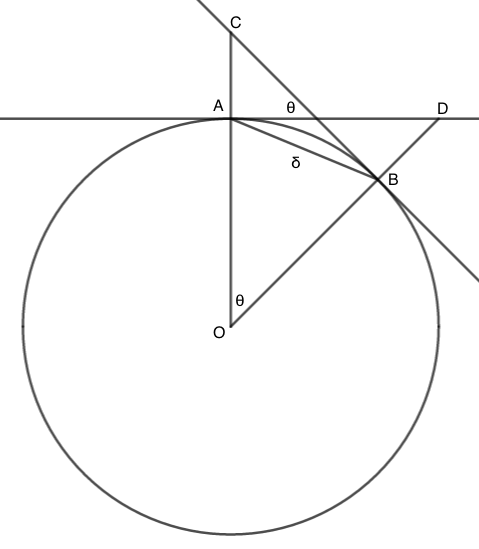
\includegraphics[width=\textwidth]{Circle-1.png}
    \caption{Drawing for Theorem 3.2.2}
  \end{subfigure}
  %
  \begin{subfigure}[b]{0.32\textwidth}
    \centering
    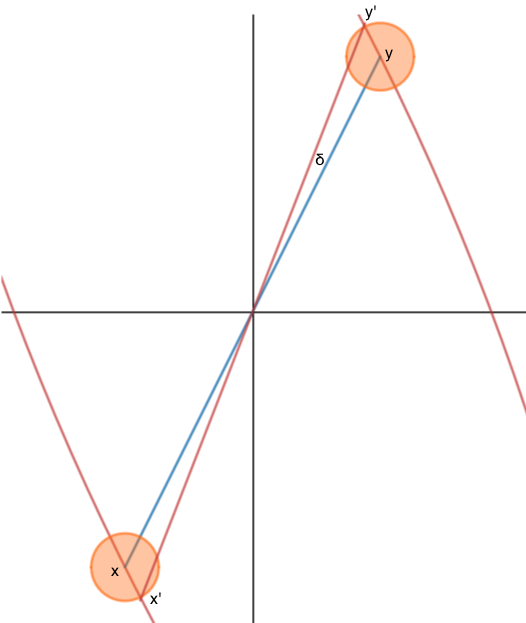
\includegraphics[width=\textwidth]{convex-1.png}
    \caption{Drawing for Theorem 3.2.3}
  \end{subfigure}
  %
  \begin{subfigure}[b]{0.32\textwidth}
    \centering
    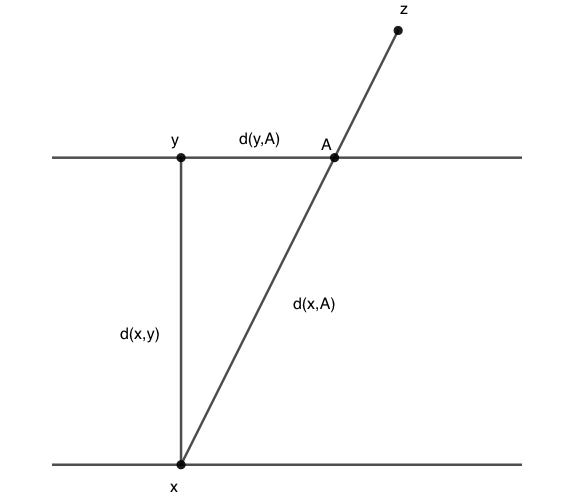
\includegraphics[width=\textwidth]{line-1.png}
    \caption{Drawing for Lemma 3.2.1}
  \end{subfigure}  
\end{figure}

\begin{theorem}
If $K\subset \mathbb{R}^2$ is compact and convex, then $R_K(\theta)$ is continuous.
\end{theorem}
\begin{proof}
For let $K$ be compact and convex, and without loss of generality suppose it contained within the unit disc and contains the origin. Let $\theta\in (0,2\pi)$ be given and let $\ell_{\theta}$ be a line through the origin making an angle $\theta$ with the horizontal. Let $x=(x_1,x_2),y=(y_1,y_2)\in K$ be such that $W_{\ell_{\theta}}(K) = d(x,y)$. Such points exist as $K$ is compact. Let $\varepsilon>0$ be given. About $x$, consider $B_{\frac{\varepsilon}{2}}(x)$, and similarly $B_{\frac{\varepsilon}{2}}(y)$. Neither of these are empty, as $K$ is convex. Let $x',y'\in K\cap(B_{\frac{\varepsilon}{2}}(x)\cup B_{\frac{\varepsilon}{2}}(y))$ be such that $d(x',y')$ is maximized. As this set is compact, such points exist. Let $\delta = \min\{|\theta-\frac{x_2'}{\sqrt{x_1'^2+x_2'^2}}|,|\theta-\frac{y_2'}{\sqrt{y_1'^2+y_2'^2}}|\}$. Then for $|\theta-\theta_0|<\delta$, $d(x,y)-\varepsilon \leq W_{\ell_{\theta_0}}(K)\leq d(x,y)+\varepsilon$, and thus $|W_{\ell_\theta}(K)-W_{\ell_{\theta_0}}(K)| < \varepsilon$.
\end{proof}

\begin{lemma}
If $K$ is a compact subset of $\mathbb{R}^2$ and $x,y\in K$ such that $d(x,y)=D(K)$, then the lines perpendicular to $\overline{xy}$ at $x$ and $y$ contain all of $K$ in between.
\end{lemma}
\begin{proof}
Suppose not. Let $\overline{X}$ be the line perpendicular to $\overline{xy}$ containing point $x$, and similarly define $\overline{Y}$. Suppose there is a point $z\in K$ that falls on the exterior of the region $\mathcal{U} = \{(x,y)\in \mathbb{R}^2: (x,y)\ \textrm{Lies Between } \overline{X}\ \textrm{and } \overline{Y}\}$. Note that $d(x,z)\ne d(y,z)$, as then $z$ would line between these two lines. Suppose $d(y,z)<d(x,z)$. Where the line $\overline{xz}$ cuts $\overline{Y}$ denote as $A$. But then $d(x,z) > d(x,A) = \sqrt{d(y,A)^2+d(x,y)^2}\geq d(x,y)$. A contradiction as $d(x,y) = D(K)$. Thus $z\in \mathcal{U}$.
\end{proof}

\begin{theorem}
If $K\subset \mathbb{R}^2$ is compact and convex, then there are points $x,y\in K$ such that $\check{W}(K)=d(x,y)$.
\end{theorem}
\begin{proof}
As $f_K(\theta)$ is continuous for convex compact set, and as it is continuous on a compact set $[0,2\pi]$, it attains its maximum. Let $\theta$ be such a maximum. Let $\ell_{\theta}$ be the line through the origin which makes an angle $\theta$ with the horizontal axis and consider set $K_{\ell_{\theta}}$. As $K$ is compact and $\ell_{\theta}$ is closed, $K_{\ell_{\theta}}$ is compact. Then $W=\{d(x,y):x,y\in K_{\ell_{\theta}}\}$ is bounded, has a least upper bound, and therefore there are points $x,y \in K$ such that $\check{W}(K)=d(x,y)$.
\end{proof}

\begin{theorem}
If $K$ is a compact convex set of $\mathbb{R}^2$, then $D(K) = \check{W}(K)$.
\end{theorem}
\begin{proof}
As $K$ is compact, $D(K)$ and $\check{W}(K)$ exists and there are points $x,y$ such that $d(x,y) = D(K)$ and points $x',y'$ such that $d(x',y') = \check{W}(K)$. Suppose $d(x',y')> d(x,y)$. A contradiction, as $d(x,y)$ is the diameter of $K$. So $d(x,y) \geq d(x',y')$. Now suppose $d(x,y)>d(x',y')$. But as $d(x',y')= \check{W}(K)$, $d(x',y')$ is the greatest length of any line segment that terminates in $K$ and such that perpendiculars at these terminating points contain all of $K$. But as $d(x,y)=D(K)$, the lines perpendicular to $\overline{xy}$ at $x$ and $y$ contain all of $K$, a contradiction. Thus $d(x',y') \geq d(x,y)$. But it was just showed that $d(x,y)\geq d(x',y')$. Thus, $d(x,y) = d(x',y')$. $D(K) = \check{W}(K)$.
\end{proof}

\begin{definition}
If $Q$ is a convex polygon with interior (That is, positive area) in $\mathbb{R}^2$, then the perimeter of $Q$ is the sum of the lengths of its edges. 
\end{definition}

\begin{definition}
The perimeter of a line segment $e$ is $P(e) = 2|e|$.
\end{definition}

\begin{remark}
This is for the sake of continuity. If we take a rectangle of length $|e|$ and width $\frac{1}{n}$, then the perimeter is $2|e|+\frac{2}{n} \rightarrow 2|e|$ as $n\rightarrow \infty$. Thus, for the puprose of continuity we define the perimeter of line segments to be twice their length.
\end{remark}

\begin{theorem}[Cauchy's Perimeter Theorem]
If $K$ is a compact convex subset of the plane, then $P(K) = \pi W(K)$.
\end{theorem}
\begin{proof}
Suppose that $Q$ is a convex polygon with edges $e_1,\hdots, e_n$. At each $e_i$, let $\theta_i$ be the angle made with $e_i$ and the horizontal axis of $\mathbb{R}^2$. The mean width is $W(Q) = \frac{1}{2\pi}\int_{0}^{2\pi} W_{\ell_\theta}(Q)d\theta = \frac{1}{2\pi} \int_{0}^{2\pi} \frac{1}{2} \sum_{i=1}^{n} |e_i||\cos(\theta-\theta_i)|d\theta = \frac{1}{4\pi}\sum_{i=1}^{n} |e_i|\int_{0}^{2\pi} |\cos(\theta-\theta_i)|d\theta = \frac{1}{\pi} \sum_{i=1}^{n} |e_i| = \frac{1}{\pi} P(Q)$. Thus, $P(Q) = \pi W(Q)$. For any convex compact subset $K\subset \mathbb{R}^2$, we may find a polygon $Q$ that approximates the boundary with a perimeter $P(Q)$ that is as close to $P(K)$ and a width $W(Q)$ as close to $W(K)$ as desired. That is, for all $n\in \mathbb{N}$, we can obtain a polynomial $Q_n$ such that $\max\{|W(Q_n)-W(K)|,|P(K)-P(Q_n)|\}< \frac{1}{n}$. Then $|P(K)-\pi W(K)| = |P(K) - P(Q_n)+P(Q_n)-\pi W(Q_n)+\pi W(Q_n)-\pi W(K)| \leq |P(K)-P(Q_n)|+|P(Q_n)-\pi W(Q_n)|+\pi|W(Q_n)-W(K)| < \frac{1}{n} + 0 + \frac{\pi}{n} = \frac{1+\pi}{n} \rightarrow 0$. Thus, $P(K) = \pi W(K)$ for arbitrary convex compact subsets of the plane.
\end{proof}
 
\begin{theorem}
There exist compact path-connected sets $K\subset \mathbb{R}^2$ such that $P(K) \ne \pi W(K)$.
\end{theorem}
\begin{proof}
Consider the set $K = \{(x,y) \in \mathbb{R}^2: x^2+y^2=1, y\geq 0\}$. Then $P(K) = 2\pi$, but \\ $W(K) = \pi(\pi+2)$. To see this, consider the set $\mathcal{K} = \{(x,y)\in \mathbb{R}^2: x^2 + y^2 \leq 1, y\geq 0\}$. This is convex and has perimeter $\pi+2$ and therefore $W(\mathcal{K}) = \pi(\pi+2)$. But, as the image shows, $W(K) = W(\mathcal{K})$. That is, $W_{\ell_{\theta}}(K)$ is the length of the line segment $\overline{AB}$, as is $W_{\ell_{\theta}}(\mathcal{K})$. Therefore the averages $W(K)$ and $W(\mathcal{K})$ are the same. Thus, $P(K) \ne \pi W(K)$.
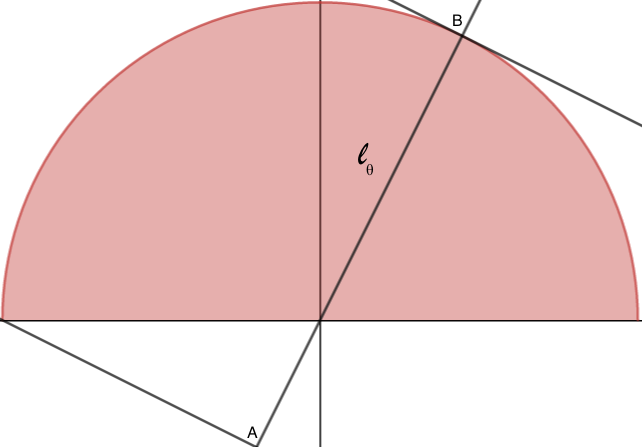
\includegraphics[scale=0.3]{semicircle-1.png}
\end{proof}

\begin{definition}
A functional $f$ with respect to subset inclusion is said to be monotonic on a family of sets $\mathscr{P}$ if and only if $f(K)\leq f(L)$ for all $K,L \in \mathscr{P}$ such that $K\subset L$.
\end{definition}

\begin{theorem}
If $K\subset L \in \mathscr{K}_2$, then $W_{\ell}(K) \leq W_{\ell}(L)$.
\end{theorem}
\begin{proof}
For let $\pi_{\ell}:\mathbb{R}^2 \rightarrow \ell$ be the orthogonal projection map of $\mathbb{R}^2$ to $\ell$. Then $\pi_{\ell}(K)\leq \pi_{\ell}(L)$ as $K\subset L$, and thus $W_{\ell}(K)\leq W_{\ell}(L)$.
\end{proof}

\begin{theorem}
If $K\subset L\in \mathscr{K}_2$, then $W(K)\leq W(L)$.
\end{theorem}
\begin{proof}
For $W_{\ell}(K)\leq W_{\ell}(L)$, and thus $W(K)=\frac{1}{2\pi}\int_{0}^{2\pi}W_{\ell_{\theta}}(K)d\theta \leq \frac{1}{2\pi}\int_{0}^{2\pi}W_{\ell_{\theta}}(L)d\theta=W(L)$.
\end{proof}

\begin{theorem}
If $K\subset L\in \mathscr{K}_2$, then $X_{\ell}(K)\leq X_{\ell}(L)$.
\end{theorem}
\begin{proof}
For if $x\in \ell\cap K$, then $x\in \ell\cap L$, and thus $X_{\ell}(K)=\mu(\ell\cap K) \leq \mu(\ell\cap L)=X_{\ell}(L)$.
\end{proof}

\begin{theorem}
If $K\subset L\subset \mathscr{K}_2$, then $D(K)\leq D(L)$.
\end{theorem}
\begin{proof}
For suppose not. Suppose $D(K)>D(L)$. Then, there are points $x,y\in K$ such that $d(x,y)> \sup\{d(x',y'):x',y'\in L\}$. But as $K\subset L$, $x,y\in L$ and thus $d(x,y) \not> \sup\{d(x',y'):x',y'\in L\}$. Thus, $D(K)\leq D(L)$.
\end{proof}

\begin{theorem}
If $K\subset L \subset \mathscr{K}_2$, then $R_K\leq R_L$.
\end{theorem}
\begin{proof}
For suppose not. Suppose $R_K>R_L$. But as $K\subset L$, either this circle contains all of $L$ as well or it doesn't. But then $R_L \not<R_K$. Thus, $R_L\geq R_K$.
\end{proof}

\begin{theorem}
If $K\subset L \in \mathscr{K}_2$, then $r_K \leq r_L$.
\end{theorem}
\begin{proof}
For suppose not. Suppose $r_K> r_L$. But as the inscribed circle of radius $r_K$ fits entirely in $K$, and $K\subset L$, then it fits inside of $L$. But then $r_K \not > r_L$. Thus, $r_L \geq r_K$.
\end{proof}

\begin{theorem}
If $K,L\in \mathscr{K}_2$ and $K\subset L$, then $P(K)\leq P(L)$.
\end{theorem}
\begin{proof}
As $K\subset L\in  \mathscr{K}_2$, $W(K)\leq W(L)$. As $K$ and $L$ are convex, $P(K)=\pi W(K)$ and $P(L)=\pi W(L)$. Thus, $P(K) \leq \pi W(L) = P(L)$. Therefore, $P(K)\leq P(L)$.
\end{proof}

\begin{theorem}
There exists sets $K,L\subset \mathbb{R}^2$ such that $L$ is convex, $K\subset L$, yet $P(K)>P(L)$.
\end{theorem}
\begin{proof}
For let $L = \{(x,y)\in \mathbb{R}^2: x^2 + y^2 \leq 1\}$. Then $P(L) = 2\pi$. Let $K = \{(x,y)\in \mathbb{R}^2: -\sqrt{2}x\leq y \leq \sqrt{2}x,\frac{-1}{\sqrt{3}} \leq x \leq \frac{1}{\sqrt{3}} \lor \sqrt{2}x\leq y \leq -\sqrt{2}x,\frac{-1}{\sqrt{3}} \leq x \leq \frac{1}{\sqrt{3}} \}$. $P(K) = 4(1+ \sqrt{\frac{2}{3}}) \approx 7.26>2\pi$.
\end{proof}

\begin{figure}[H]
  \begin{subfigure}[b]{0.49\textwidth}
     \centering
    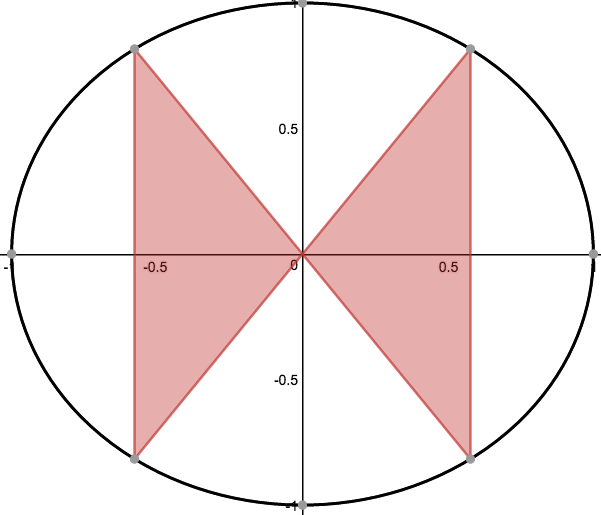
\includegraphics[width=\textwidth]{Circles-3.png}
    \caption{Drawing for Theorem 3.2.15}
  \end{subfigure}
  %
  \begin{subfigure}[b]{0.49\textwidth}
    \centering
    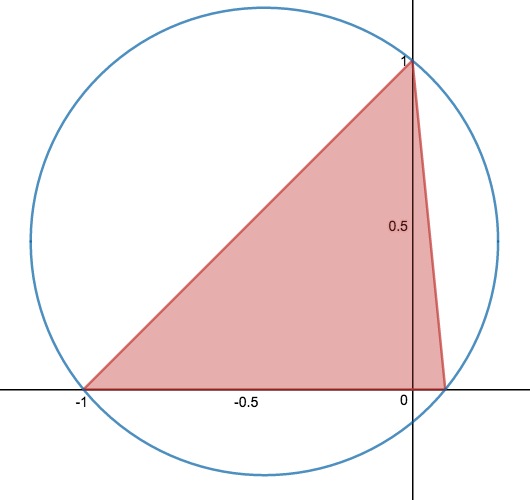
\includegraphics[width=\textwidth]{Circle-4.png}
    \caption{Drawing for Theorem 3.2.16}
  \end{subfigure}
\end{figure}


\begin{theorem}
There exist compact convex sets in $\mathbb{R}^2$ such that $D(K) < 2R_K$.
\end{theorem}
\begin{proof}
For consider the set $K=\{(x,y)\in \mathbb{R}^2: [0\leq y\leq x+1 \land x\geq 0]\lor [0\leq y\leq -10x+1\land x\geq 0]\}$. From Euclid, the smallest circle containing this triangle is the one defined by the three vertices (Three points define a triangle). This circle has the formula $(x+0.45)^2+(y-0.45)^2 = (0.45)^2 +(0.45+\frac{1}{10})^2$. Thus, $2R_K = \sqrt{0.45^2 +(0.45+\frac{1}{10})^2} > \sqrt{2} = D(K)$.
\end{proof}

\begin{theorem}
If $K$ is a compact convex set in $\mathbb{R}^2$, then $D(K) \leq 2R_K$.
\end{theorem}
\begin{proof}
For suppose not. Suppose $D(K) > 2R_K$. As $K$ is compact, there are points $x$ and $y$ in $K$ such that $d(x,y)=D(K)$. But then $d(x,y)>2R_K$, and thus at least one of $x$ or $y$ is not contained in the circle. A contradiction. Thus $D(K)\leq 2R_K$.
\end{proof}

\begin{theorem}
If $K$ is a compact convex set in $\mathbb{R}^2$, then $2\pi r_K \leq P(K)$.
\end{theorem}
\begin{proof}
From Calculus of Variations we know that the circle maximizes the area contained with a set of perimeter $p$. As the inscribed circle has perimeter $2\pi r_K$ and as the circle is a subset of $K$, it is true that $A(K)$ is greater than or equal the area of the circle. Thus, $P(K)\geq 2\pi r_K$.
\end{proof}

\begin{theorem}
For a compact convex set of $\mathbb{R}^2$, $P(K) \leq 2\pi R_K$.
\end{theorem}
\begin{proof}
As $K$ is convex, $P(K) = \pi W(K) \leq \pi \check{W}(K) = \pi D(K) \leq 2\pi R_K$.
\end{proof}

\begin{theorem}
If $K$ is a compact and convex subset of $\mathbb{R}^2$, then $2D(K)\leq P(K)$.
\end{theorem}
\begin{proof}
Suppose not. Suppose $2D(K) >P(K)$. As $K$ is compact and convex, there exist points $x,y\in K$ such that $d(x,y) = D(K)$. But as $K$ is convex, the line contained between $x,y$ in contained in $K$. Thus, $P(\overline{xy}) = 2D(K)$. But as $\overline{xy}\subset K$, $P(K)>P(\overline{xy})$, a contradiction. Thus, $2D(K) \leq P(K)$.
\end{proof}
%
\begin{theorem}
There exist compact convex subsets of $\mathbb{R}^2$ such that $2D(K) = P(K)$.
\end{theorem}
\begin{proof}
For take a straight line segment of length $\ell$. Then $D(K) = \ell$, $P(K) = 2\ell$, and thus $2D(K) = P(K)$.
\end{proof}
%
\begin{theorem}
If $K$ is a compact convex subset of $\mathbb{R}^2$, then $P(K) \leq \pi D(K)$.
\end{theorem}
\begin{proof}
From Cauchy's Perimeter theorem, $P(K) = \pi W(K) \leq \pi \check{W}(K) = \pi D(K)$.
\end{proof}
%
\begin{theorem}
For a compact convex subset $K$ of $\mathbb{R}^2$, $P(K) = \pi D(K)$ if and only if $W_{\ell}(K)$ is a constant.
\end{theorem}
\begin{proof}
For then $\frac{1}{2\pi} \int_{0}^{2\pi} W_{\ell_{\theta}}(K) d\theta = \check{W}(K)$. But as $W_{\ell_{\theta}}(K)$ is continuous for compact convex bodies, it must be true that $W_{\ell_{\theta}}(K) = \check{W}(K)$ for all $\ell_{\theta}$. Thus, $K$ is of constant width.
\end{proof}
%
\begin{remark}
There are many types of shapes that have constant width besides discs. The Reuleaux Triangle is such an example.
\end{remark}
%
Triangles are the simplest convex bodies in the plane other than points and lines. Any convex polygon can be written as the union of triangles with disjoint interiors. 
%
\begin{theorem}
If $\Delta_s$ is an equilateral triangle with edge length $s$, then $\Delta_s$ has the following properties:
\begin{enumerate}
\begin{multicols}{5}
\item $A(\Delta_s) = \frac{\sqrt{3}}{4}s^2$
\item $P(\Delta_s) = 3s$
\item $W(\Delta_s) = \frac{3s}{\pi}$
\item $R_{\Delta_s} = \frac{1}{\sqrt{3}}s$
\item $r_{\Delta_s} = \frac{1}{2\sqrt{3}}s$
\end{multicols}
\end{enumerate}
\end{theorem}
%
\begin{proof}
In order:
\begin{enumerate}
\item From Pythagoras, $A(\Delta_s) =2\times\big[\frac{1}{2}(\frac{1}{2}s)(\frac{\sqrt{3}}{2}s)\big] = \frac{\sqrt{3}}{4}s^2$
\item There are three edges, each of length $s$, and thus $P(\Delta_s) = 3s$.
\item $W(\Delta_s) = \frac{1}{\pi}P(\Delta_s) = \frac{3s}{\pi}$
\item The circumcircle gives the following equations:
\begin{enumerate}
\item $R_{\Delta_s}^2=\frac{s^2}{4}+h^2$
\item $h+R_{\Delta_s} = \frac{\sqrt{3}}{2}s$
\end{enumerate}
This has solution $R_{\Delta_s}=\frac{1}{\sqrt{3}}s$
\item $r_{\Delta_s} = \frac{R_{\Delta_s}}{2}= \frac{1}{2\sqrt{3}}s$
\end{enumerate}
\end{proof}

\begin{theorem}
If $T$ is a triangle in the plane, then there is a linear transformation $\psi$ such that $\psi T$ is equilateral.
\end{theorem}
\begin{proof}
For let $T$ be a triangle with vertices $a=(x_1,y_1)$, $b=(x_2,y_2)$, $c=(x_3,y_3)$. Let $A = d(b,c)$, $B=d(a,c)$, and $C=d(a,b)$. Suppose If $A=B=C$, we are done. Thus, suppose $C\geq B >A$. At point $a$ and with radius $C$, construct the circle $b,c',d$, and point $b$ and with radius $C$, construct the circle $a,c',e$. If we can shift $c$ to $c'$ in a linear fashion, we are done. Let $\psi =$
\end{proof} 

\begin{theorem}
If $T$ is a triangle with edges $a,b,c$ and opposite angles $\alpha,\beta,\gamma$, respectively, then $A(T) = \frac{\sin(\alpha)}{2}bc = \frac{\sin(\beta)}{2}ac = \frac{\sin(\gamma)}{2}ab$
\end{theorem}
\begin{proof}
Suppose the triangle is acute. The proof is symmetric for all sides, so we prove it for just $\alpha$. Note that the perpendicular $h$ dropped from the vertex of $a$ onto $b$ satisfies $h^2+\ell_1^2 = c^2$ and $h^2+\ell_2^2 = a^2$, where $\ell_1+\ell_2 = b$. Then $\sin(\alpha) = \frac{h}{c}$ and $A(T) = \frac{1}{2}h\ell_1 + \frac{h}{2}h\ell_2 = \frac{h}{2}(\ell_1+\ell_2)h = \frac{1}{2}bh = \frac{1}{2}bc\sin(\alpha)$. An identical argument works for obtuse triangles.
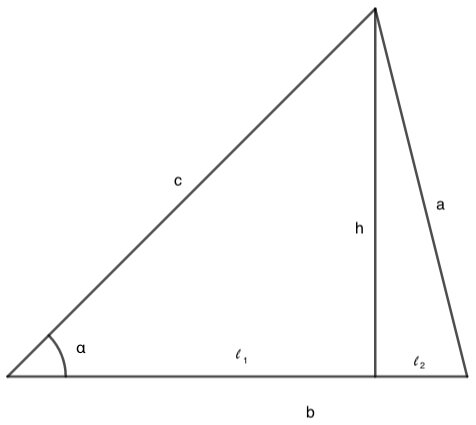
\includegraphics[scale=0.3]{triangle-1.png}
\end{proof}

\begin{corollary}[The Law of Sines]
For a triangle with edges $a,b,c$ and opposite angles $\alpha,\beta,\gamma$, $\frac{\sin(\alpha)}{a} = \frac{\sin(\beta)}{b} = \frac{\sin(\gamma)}{c}$
\end{corollary}
\begin{proof}
From the previous theorem, divide by $\frac{abc}{2}$ to obtain the result.
\end{proof}

\begin{theorem}[The Law of Cosines]
Given a triangle with lengths $a,b,c$ and opposite edges $\alpha,\beta,\gamma$, $c^2=a^2+b^2-2ab\cos(\gamma)$.
\end{theorem}
\begin{proof}
If $\gamma=\frac{\pi}{2}$, this is Pythagoras' Theorem. Thus, suppose $0<\gamma < \frac{\pi}{2}$. Where $c$ and $a$ meet, drop a perpendicular onto $c$ and call this $h$. $h$ satisfies $h^2+\ell_1^2 = c^2$ and $h^2+\ell_2^2=a^2$ from Pythagoras' Theorem, where $\ell_1+\ell_2 = b$. But $\ell_2 = a\cos(\gamma)$, so $\ell_1 = b-a\cos(\gamma)$. Thus $c^2 = h^2 + b^2 +a^2\cos^2(\gamma)-2ab\cos(\gamma)$. But $h = a\sin(\gamma)$. Thus, $c^2 = b^2 + a^2 \cos^2(\gamma)+\sin^2(\gamma)-2ab\cos(\gamma) = b^2 + a^2(\sin^2(\gamma)+\cos^2(\gamma))-2ab\cos(\gamma) = a^2 + b^2 -2ab\cos(\gamma)$. A similar construction is done if $\frac{\pi}{2}<\gamma < \pi$.
\end{proof}

\begin{theorem}
Given a triangle $\Delta$ with lengths $a\leq b\leq c$, $D(\Delta)=c$.
\end{theorem}
\begin{proof}
At the midpoint of $c$, and with radius $c$, construct a circle. This circle contains the entirety of $\Delta$, and thus for all points $x,y\in \Delta$, $d(x,y)\leq c$. Thus, $c=D(\Delta)$.
\end{proof}

\begin{theorem}[Heron's Formula]
For a triangle with lengths $a,b,c>0$, $A(T)^2 = \frac{1}{16}(a+b+c)(-a+b+c)(a-b+c)(a+b-c)$.
\end{theorem}
\begin{proof}
For $A(T) = \frac{1}{2}ab \sin(\gamma) = \frac{1}{2}ab\sqrt{1-\cos^2(\gamma)} = \frac{1}{4}\sqrt{4a^2 b^2 - (a+b-c)^2}=\\ \frac{1}{4}\sqrt{(2ab-(a^2+b^2-c^2))(2ab+(a^2+b^2+c^2))} = \frac{1}{4}\sqrt{(c^2-(a-b)^2)((a+b)^2-c^2)} = \\ \frac{1}{4}\sqrt{(a+b+c)(-a+b+c)(a-b+c)(a+b-c)}$. Squaring this gives the result.
\end{proof}

\begin{theorem}
For any triangle $\Delta$, $r_{\Delta}P(\Delta) = 2A(\Delta)$.
\end{theorem}
\begin{proof}
For let $\Delta$ has sides $a,b,c$, with opposite angles $\alpha, \beta, \gamma$, respectively. Then $A(\Delta) = \frac{ab}{2}\sin(\gamma)$ and $P(\Delta)=a+b+c$. Thus, $\frac{2A(\Delta)}{P(\Delta)} = \frac{ab\sin(\gamma)}{a+b+c}$. But this is the radius of the incircle of $\Delta$. Therefore, etc.
\end{proof}

\begin{theorem}[Viviani's Theorem: Page 17]
\end{theorem}

\begin{theorem}
There exist convex polygon's such that the inradius is not unique.
\end{theorem}
\begin{proof}
For consider the rectangle $[0,2]\times [0,1]$. The diameter of any circle that sits inside this body must be at most $1$, and thus the radius is at most $\frac{1}{2}$. However, there are multiple circles that achieve this. For example $(x-\frac{1}{2})^2+(y-\frac{1}{2})^2=\frac{1}{2}$ and $(x-\frac{3}{2})^2+(y-\frac{3}{2})^2=\frac{1}{2}$.
\end{proof}

\begin{theorem}
For an acute triangle, $\frac{2(A)}{abc} = \frac{1}{R_T}$.
\end{theorem}

\begin{theorem}
If $\Delta$ is a triangle with vertices $A,B,C$ and sides $a,b,c$, then given a circle that contains $A,B,C$, the radius of this circle $R$ satisfies $\frac{1}{R} =\frac{2A(\Delta)}{abc}$
\end{theorem}

\begin{definition}
If $K\in \mathscr{K}_2$, then $-K = \{-x:x\in K\}$.
\end{definition}

\begin{theorem}
If $K\in \mathscr{K}_2$, then $W_{\ell}(K) = W_{\ell}(-K)$.
\end{theorem}
\begin{proof}
For let $x,y\in K$ be such that $d(x,y) = W_{\ell}(K)$. Then $d(-x,-y) = W_{\ell}(-K) = d(x,y)$. Therefore, etc.
\end{proof}

\begin{theorem}
There exist sets $K$ and $L$ such that $W_{\ell}(K)<W_{\ell}(L)$ for all $\ell$ yet $K\not\subset L$ for any translation or rotation of $K$.
\end{theorem}

\begin{definition}
For $K\in \mathscr{K}$ and unit vector $u$, $\bar{X}_{u}(K)$ is the mean value of $X_{\ell}(K)$ over all lines $\ell$ parallel to $u$ such that $X_{\ell}(K)>0$.
\end{definition}

\begin{theorem}
For $K\in \mathscr{K}_2$, $\bar{X}_{u}(K) = W_{\ell}(K)=A(K)$.
\end{theorem}
%
\chapter{Some More Stuff}
\section{On the Quotients of Primes}
\begin{theorem}
The set of rational numbers $\frac{p}{q}$ where $p$ and $q$ are prime is dense in $\mathbb{R}^{+}$.
\end{theorem}
\begin{proof}
If $x=0$, from Euclid we have $\frac{1}{p_n}\rightarrow 0$, where $p_n$ is the $n^{th}$ prime. Let $x\in\mathbb{R}^{+}$ be given. From the Prime Number Theorem, $\frac{p_n}{n\ln(n)}\rightarrow 1$. Let $p_{\ceil{nx}}$ be the $\ceil{nx}^{th}$ prime. Then $\frac{p_{\ceil{nx}}}{p_n}\frac{n\ln(n)}{nx\ln(nx)}\rightarrow 1$. But $\frac{n\ln(x)}{nx\ln(nx)}\rightarrow \frac{1}{x}$. Therefore $\frac{p_{\ceil{nx}}}{p_n}\rightarrow x$.
\end{proof}
%
\section{On Uniform Convergence}
%
\begin{definition}
A sequence of functions $f_n$ is said to converge point-wise on a set $A$ to a function $f$, if $\forall\varepsilon>0$ and $\forall x\in A$, there is an $N\in\mathbb{N}$ such that $n>N \Rightarrow |f(x)-f_n(x)|<\varepsilon$.
\end{definition}

\begin{definition}
A sequence of functions $f_n$ converge uniformly on a set $A$ to $f$ if and only if $\forall \varepsilon>0$ $\exists N\in\mathbb{N}$ such that $\forall x \in A$ and $n>N$, $|f(x) -f_n(x)|<\varepsilon$.
\end{definition}

\begin{definition}
A sequence of functions $f_n$ are point-wise equicontinuous on a set $A$ if and only if $\forall \varepsilon>0, \forall x \in A,\ \exists \delta>0\ \forall n\in\mathbb{N}|\ |x-x_0|<\delta \Rightarrow |f_n(x) - f_n(x_0)|<\varepsilon$.
\end{definition}

\begin{definition} A sequence of functions $f_n$ are uniformly equicontinuous on a set A if and only if $\forall\varepsilon>0,\ \exists \delta>0\ \forall x\in A\ \forall n\in\mathbb{N}|\ |x-x_0|<\delta \Rightarrow |f_n(x) - f_n(x_0)|<\varepsilon$.
\end{definition}

\begin{definition} A subset $A$ of the real line is open if $\forall x\in A,\ \exists r>0|\ \forall y \in (x-r,x+r),\ y\in A$.
\end{definition}

\begin{definition}
An open cover $\Delta$ of a set $A\subset S$ is a set of open subsets $A_k\subset S$, such that $A \subset \cup_{k\in I} A_k$, where $I$ is some index, countable or uncountable.
\end{definition}

\begin{definition}
A set $A$ is said to be compact if and only if for all open coverings $\Delta$ there is a finite sub-cover $\Delta_0\subset \Delta$, such that $A\subset \cup_{A_k \in \Delta_0} A_k$.
\end{definition}

\begin{theorem}[Heine-Borel Theorem]
Any closed-bounded subset of the real line is compact. 
\end{theorem}
\begin{proof}
For let $A$ be a closed and bounded subset of $\mathbb{R}$ with least upper bound $b$ and greatest lower bound $a$. Let $\Delta$ be an open covering, and let $X$ be the set of points $y\in A$ such that for all $s<y$ such that $s\in A$, there is a finite refinement of $\Delta$ which covers these points. $X$ is non-empty, as $a\in X$. The set $X$ is bounded, as for all points $y\in X$ we have that $a\leq y \leq b$. As bounded sets have a least upper bound, let $x$ be the least upper bound. Suppose $x<b$. As $x\in [a,b]$, there exists an element $A_k$ of $\Delta$ such that $x \in A_k$. But as $A_k$ is open and therefore there is an $r>0$ such that $y\in (x-r,x+r)\Rightarrow y \in A_k$. But then $y=x + \frac{r}{2} > x$ and $y\in A_k$. Therefore x is not the least upper bound as we have found an element in $X$ greater than $x$. Therefore $x\not<b$. And thus $x=b$.
\end{proof}

\begin{theorem}
If a sequence of functions are point-wise equicontinuous on a closed and bounded set, then they are uniformly equicontinuous.
\end{theorem}
\begin{proof}
For let $A$ be a closed bounded subset of $\mathbb{R}$, and let $f_n(x)$ be a sequence of point-wise equicontinuous functions on $A$. As the set is closed and bounded, it is compact by the Heine-Borel theorem. Let $\varepsilon>0$ be given. For $x\in A$, define the function $\delta(x) = \min\{\sup\{\delta>0:\ |x-x_0|<\delta,\ x_0\in A \Rightarrow |f_n(x)-f_n(x_0)|<\frac{\varepsilon}{2}, \forall n\in\mathbb{N}\},b-a\}$. Construct the open covering $\mathcal{U}$ as follows: $\mathcal{U} = \{(x-\delta(x),x+\delta(x)):\ x\in A\}$. This is an open covering, as every set in $\mathcal{U}$ is open, and for all $x\in A$, $x\in(x-\delta(x),x+\delta(x))\in\mathcal{U}$. But as $A$ is compact, there is a finite sub-cover. Let $a=x_0<x_1<...<x_{n-1}<x_n=b$ be the centers of the remaining open sets in the sub-cover. Further refine this sub-covering as follows: If $(x_j-\delta(x_j),x_j+\delta(x_j))\subset (x_k-\delta(x_k),x_k+\delta(x_k))$ for $j\ne k$, then remove it from the sub-cover as it is superfluous. We now have a set of points $a=a_0<z_1<...<z_{N-1}<z_N=b$ such that $A \subset \cup_{i=0}^{N} (z_i-\delta(z_i),z_i+\delta(z_i))$. Let $\delta = \min\{\delta(z_0),...,\delta(z_N),\delta(b), \frac{(a+\delta(a)) - (z_1-\delta(z_1))}{2}, ..., \frac{(z_{N-1} + \delta(z_{N-1})) - (b-\delta(b))}{2}\}$. That is, $\delta$ is the smallest of the $\delta(z_i)$, or half of the smallest intersection of two consecutive intervals. Let $x\in A$ be arbitrary. If $(x-\delta,x+\delta)$ is contained entirely in one of the $(z_i-\delta(z_i),z_i+\delta(z_i))$ sets, then we have that $|x-x_0|<\delta \Rightarrow |x-x_0| <\delta(z_i) \Rightarrow |f_n(x)-f_n(x_0)|<\frac{\varepsilon}{2}$ for all $n\in\mathbb{N}$. Suppose that $(x-\delta,x+\delta)$ is contained in two of the $(x-\delta(z_i),x+\delta(z_i))$ sets. Note, it cannot be in three or more as we have refined the sub-cover in such a manner as to prevent this. Let $y$ be the center of the intersection of these two sets. Then we have that for $|x-x_0|<\delta$, then $|f_n(x)-f_n(x_0)| = |f_n(x) - f_n(y) + f_n(y) - f_n(x_0)| \leq |f_n(x) - f_n(y)| + |f_n(y) - f_n(x_0)|$. But $|x-y|$ and $|x_0-y|$ are less than $\frac{(z_i + \delta(z_i))-(z_{i+1}-\delta(z_{i+1}))}{2}$ apart, and therefore $|f_n(x) - f_n(y)|<\frac{\varepsilon}{2}$, and $|f_n(y) - f_n(x_0)| < \frac{\varepsilon}{2}$. Therefore, $|f_n(x) - f_n(x_0)|<\varepsilon$. And as $x$ is arbitrary, $f_n(x)$ is uniformly equicontinuous.
\end{proof}

\begin{theorem} If a sequence of point-wise equicontinuous functions converge, then the limit is point-wise continuous.
\end{theorem}
\begin{proof}
For let $f_n:A\rightarrow \mathbb{R}$ be equicontinuous, $\varepsilon>0$ and $x\in A$ be given. Choose $\delta>0$ to satisfy the criterion of equicontinuity at $x$. Let $x_0$ be an arbitrary point in $(x-\delta,x+\delta)\cap A$. It suffices to show that $|f(x) - f(x_0)|<\varepsilon$. As $f_n \rightarrow f$ we have that $\exists N_1 \in\mathbb{N}$ such that $n>N_1\Rightarrow |f(x) - f_n(x)|<\varepsilon$. We also have that $\exists N_2 \in \mathbb{N}$ such that $n>N_2 \Rightarrow |f(x_0)-f_n(x_0)|<\varepsilon$. Let $N=\max\{N_1,N_2\}+1$. But we have that $|f(x) - f(x_0)| = |f(x) - f_N(x) + f_N(x)-f_N(x_0) + f_N(x_0) - f(x_0)|\leq |f(x) - f_n(x)| + |f_n(x)-f_n(x_0)| + |f_n(x_0) - f(x_0)| < 3\varepsilon$. $f$ is continuous.
\end{proof}

\begin{theorem}
If $f_n \rightarrow f$ on a closed bounded subset of $\mathbb{R}$, and if $f_n$ is equicontinuous, then the convergence is uniform.
\end{theorem}
\begin{proof}
Let $A$ be a closed bounded subset of $\mathbb{R}$, $f_n(x)$ a sequence of equicontinuous functions, and let $\varepsilon>0$ be given. As $f_n(x)$ is equicontinuous on a closed bounded set, it is uniformly equicontinuous. But the limit of equicontinuous functions is continuous. Let $\delta>0$ be such that, $\forall x\in A$, $\forall n\in\mathbb{N}$, $|x-x_0|<\delta, x_0\in A \Rightarrow |f_n(x)-f_n(x_0)|<\frac{\varepsilon}{3}$ and $|x-x_0|<\delta \Rightarrow |f(x)-f(x_0)|<\frac{\varepsilon}{3}$. Let $\mathcal{U} = \{(x-\frac{\delta}{2},x+\frac{\delta}{2}): x\in A\}$. This is an open cover of $A$ and thus there is a finite subcover. Let $x_0<x_1<\hdots<x_n$ be the centers of the finitely many sets $(x_k-\frac{\delta}{2},x_k+\frac{\delta}{2})$ that cover $A$. There is thus another finite sequence of positive integers, $N_0, N_1,... N_n$, such that $n>N_k \Rightarrow |f(x_k)-f_n(x_k)|<\frac{\varepsilon}{3}$, for $k=0,1,2,...,n$. Let $N= \max\{N_0, N_1, ..., N_n\}$.It suffices to show that, for any point $x_0 \in A$, for all $n>N$, $|f(x_0)-f_n(x_0)|<\varepsilon$. Let $x_0$ be arbitrary and let $x_k$ be the nearest point to $x_0$ in the above sequence (If there are two nearest points, pick your favorite). Then we have that, for $n>N$, $|f(x_0) - f_n(x_0)| = |f(x_0)-f(x_k)+f(x_k)-f_n(x_k)+f_n(x_k)-f_n(x_0)|\leq |f(x_k)-f(x_0)|+|f(x_k)-f_n(x_k)|+|f_n(x_k)-f_n(x_0)|<\varepsilon$. The convergence is uniform.
\end{proof}


\begin{theorem}[Integration of a Uniformly Convergent Sequence of Functions] If $f_n\rightarrow f$ uniformly on a closed bounded set $A$ with $g.u.b(A)=a$, then $\int_{a}^{x} f_n \rightarrow \int_{a}^{x} f$ uniformly on $A$.
\end{theorem}
\begin{proof}
Let $\varepsilon >0$ be given, let $b=l.u.b.(A)$, and choose $N\in\mathbb{N}$ such that $n>N\Rightarrow |f(x)-f_n(x)|<\frac{\varepsilon}{b-a}$. Then we have $|\int_{a}^{x} f_n - \int_{a}^{x} f| = |\int_{a}^{x} (f_n-f)| \leq \int_{a}^{x} |f_n-f| < \int_{a}^{x} \frac{\varepsilon}{b-a}= \frac{\varepsilon}{b-a}(x-a) \leq \varepsilon$. 
\end{proof}

\begin{theorem}[Differentiation of a Uniformly Convergent Sequence of Functions]
If $f_n'\rightarrow g$ uniformly on a closed bounded set $A$, and if $f_n \rightarrow f$ on $A$, then $f' = g$.
\end{theorem}
\begin{proof} Let $a=g.u.b.(A)$ and $b=l.u.b.(A)$. We have that $f_n(x) - f_n(a) = \int_{a}^{x}f_n' \rightarrow \int_{a}^{x}g$ uniformly. But $f_n(x)-f_n(a) \rightarrow f(x) - f(a)$. Therefore $f'(x)=\frac{d}{dx}(f(x)-f(a)) = \frac{d}{dx}\int_{a}^{x} g = g(x)$. $f' = g$.
\end{proof}

\begin{theorem}[The Product of a Uniformly Convergence Sequence and a Bounded Function]  If $f_n \rightarrow f$ uniformly, and if $g$ is a bounded function, then $f_n g \rightarrow fg$ uniformly.
\end{theorem}
\begin{proof}
For let $\varepsilon>0$ and $x$ be given, and let $g$ be a bounded function with bound $M$, and choose $N\in\mathbb{N}$ such that $n>N \Rightarrow |f(x)-f_n(x)|<\frac{\varepsilon}{M}$. Then we have that $|f(x)g(x)-f_n(x)g(x)| = |g(x)||f(x)-f_n(x)| < M|f(x)-f_n(x)| <\varepsilon$.
\end{proof}

\begin{theorem}
If $f$ is continuous on a compact set $A$, then it is uniformly continuous.
\end{theorem}
\begin{proof}
For let $\varepsilon>0$ be given, let $a=g.u.b.(A)$, $b=l.u.b.(A)$, and for $x\in A$ define $\delta(x) = \min\{\sup\{\delta>0: |x-x_0|<\delta,x_0\in A\Rightarrow |f(x)-f(x_0)|<\frac{\varepsilon}{2}\},b-a\}$. Let $\Delta = \{(x-\delta(x),x+\delta(x)):x\in A\}$. Then $\Delta$ is an open cover of $A$ and therefore there is an open subscover. Let $x_k$ be the centers of the finitely many sets $(x_k-\delta(x_k),x+\delta(x_k))$ that cover $A$. Further refine this by removing overlaps. That is, if $(x_i-\delta(x_i),x_i+\delta(x_i))\subset (x_j-\delta(x_j),x_j+\delta(x_k))$ for $i\ne j$, then remove it for it is superfluous. We thus obtain a new sequence $z_1,\hdots, z_N$ such that the intervals $(z_k-\delta(z_k),z_k+\delta(z_k))$ cover $A$. Define $\delta = \min\{\delta(z_1),\hdots,\delta(z_N), \frac{(z_0+\delta(z_0))-(z_1-\delta(z_1))}{2},\hdots,(\frac{z_{N-1}+\delta(z_{N-1}))-(z_{N}-\delta(z_{N})}{2}\}$. Let $x,x_0\in A$ such that $|x-x_0|<\delta$. Let $x_k$ be the closest point in the sequence to $x$ (If there are two such points, pick your favorite). Then $|f(x)-f(x_0)|=|f(x)-f(x_k)+f(x_k)-f(x_0)|\leq |f(x)-f(x_k)|+|f(x_k)-f(x_0)|<\varepsilon$
\end{proof}

\begin{remark}
The proof of this is a mimicry of the proof that equicontinuity on a compact set implies uniform equicontinuity.
\end{remark}

\begin{definition}
A set $A$ is called sequentially compact if given a sequence $x_n\in A$, there is a convergent subsequence $x_{n_k}$.
\end{definition}

\begin{theorem}
Compact sets of $\mathbb{R}$ are sequentially compact.
\end{theorem}
\begin{proof}
Let $A$ be a compact set in $\mathbb{R}$, and let $x_n$ be a sequence in $A$. A point $x\in A$ is the limit of a subsequence of $x_n$ if for every $\varepsilon>0$ there are infinitely many of the $x_n$ such that $|x-x_n|<\varepsilon$. Suppose there is no such point. That is, for each $x\in A$ only finitely many of the $x_n$ lie within sufficiently small $\varepsilon-$neighborhoods. Let $\varepsilon(x) = \sup\{\varepsilon>0:\textrm{Only finitely many }x_n \textrm{ lie within } \varepsilon \textrm{ of } x\}$. Define $E=\{(x-\varepsilon(x)<x+\varepsilon(x)):x\in A\}$. This is an open cover of $A$, and therefore there is a finite subcover. Thus, at least one of the finitely many intervals $(x-\varepsilon(x),x+\varepsilon(x))$ must contain infinitely many of the $x_n$, a contradiction. Thus there is a convergent subsequence.
\end{proof}

\begin{theorem}
Continuous functions on compact sets are bounded.
\end{theorem}
\begin{proof}
For suppose not. Let $f:A\rightarrow \mathbb{R}$ be a continuous function on a compact set $A$, and let $x_n$ be a sequence of points in $A$ such that $f(x_n)>n$. Such a sequence must exist as $f$ is not bounded. As $A$ is compact, there must a point $x\in A$ such that some subsequence $x_{n_k}$ that converges to $x$. Let $\varepsilon >0$. Then, as $f$ is continuous, there is a $\delta>0$ such that $|x-x_0|<\delta,\ x_0\in A\Rightarrow |f(x)-f(x_0)|<\varepsilon$. But then for all points $x_{n_k}$ such that $|x-x_{n_k}|<\delta$, $-\varepsilon<f(x_{n_k})-f(x)<\varepsilon \Rightarrow f(x)-\varepsilon < f(x_{n_k})<f(x)+\varepsilon$. A contradiction as $f(x_{n_k})$ is unbounded. Thus, $f$ is bounded.
\end{proof}

\begin{corollary}
Continuous functions on compact sets attain their maximum and minimum.
\end{corollary}
\begin{proof}
For let $f:A\rightarrow \mathbb{R}$ be a continuous function on a compact set $A$. Let $f(A) = \{y\in \mathbb{R}:\exists x\in A|\ f(x)=y\}$. (This is called the image of $A$ under $f$). As $f$ is continuous, it is bounded, and thus the set $f(A)$ is bounded. But bounded sets have an l.u.b. and a g.u.b. Therefore, etc.
\end{proof}

\begin{lemma}[Uniform Limit Theorem]
If $f_n\rightarrow f$ uniformly, and if the $f_n$ are continuous, then $f$ is continuous.
\end{lemma}
\begin{proof}
For let $\varepsilon>0$ be given and let $x\in A$. Let $N\in \mathbb{N}$ such that $n>N$ implies $|f(\chi)-f_n(\chi)|<\frac{\varepsilon}{3}$ for all $\chi\in A$. Let $\delta>0$ be chosen such that $|x-x_0|<\delta, x_0\in A\Rightarrow |f_N(x)-f_N(x_0)|<\frac{\varepsilon}{3}$. Then  $|f(x)-f(x_0)|=|f(x)-f_N(x)+f_N(x)-f_N(x_0)+f_N(x_0)-f(x_0)|\leq |f(x)-f_N(x_0)|+|f_N(x)-f_N(x_0)|+|f(x_0)-f_N(x_0)|<\varepsilon$.
\end{proof}

\begin{theorem}
If $f_ng\rightarrow fg$ uniformly on a compact set $A$, and if $g$ is continuous and positive, then $f_n\rightarrow f$ uniformly.
\end{theorem}
\begin{proof}
As $g$ is positive on a compact set, its minimum is also positive and is attained on $A$. Let $x_{min}\in A$ be such a minimum of $g$. Let $\varepsilon>0$ be given and let $N\in \mathbb{N}$ be such that for $n>N$, $|f_ng-fg|<\varepsilon\cdot g(x_{min})$. Then, $|f_ng-fg|=|g||f_n-f|\leq |g(x_{min})||f_n-f|<\varepsilon \cdot g(x_{min})\Rightarrow |f_n-f|<\varepsilon$.
\end{proof}

\begin{lemma}
If $f_n'$ is uniformly bounded, then $f_n$ is equicontinuous.
\end{lemma}
\begin{proof}
For let $M$ be such a bound for $f_n'$ and let $\varepsilon>0$ be given. Choose $\delta = \frac{\varepsilon}{M}$. Then for $x,x_0\in A$ and $|x-x_0|<\delta$, $|\int_{x_0}^{x}f_n'| =|f_n(x)-f_n(x_0)| \leq \int_{x_0}^{x}|f_n'| \leq (x-x_0)M < \varepsilon$.
\end{proof}

\begin{theorem}
If $f_n'$ is uniformly bounded, and if $f_n \rightarrow f$ on a closed and bounded subset of $\mathbb{R}$, then the convergence is uniform.
\end{theorem}
\begin{proof}
From the previous lemma, $f_n$ is equicontinuous. But a sequence of equicontinuous functions on a compact set is uniformly equicontinuous. And a sequence of uniformly equicontinuous functions that converge does so uniformly. Therefore, etc.
\end{proof}

\begin{theorem}
If $f_n \rightarrow f$, $f_n'\rightarrow g$ and if $f_n''-f_n'$ is uniformly bounded on a closed bounded set, then the convergences are uniform and $f' = g$.
\end{theorem}
\begin{proof}
Let $A$ be the closed bounded set under consideration. First note that as $f''_n - f'_n$ is uniformly bounded, $f_n'-f_n$ is equicontinuous. But as $f_n'$ and $f_n$ converge to $g$ and $f$, respectively, then $f_n'-f_n$ converges to $g-f$ uniformly. Let $M$ be a bounded for $f_n''-f_n'$. Let $a$ be the greatest lower bound and $b$ be the least upper bound of $A$. We then have that $-Me^{-a}\leq e^{-x}[f_n''(x)-f_n'(x)]=\frac{d}{dx}[e^{-x}f_n'(x)] < Me^{-a}$. That is, $\frac{d}{dx}[e^{-x}f_n'(x)]$ is uniformly bounded, and therefore $e^{-x}f_n'(x)$ is equicontinuous. But equicontinuity on a compact set implies uniform equicontinuity. As $f_n'\rightarrow g$, and $e^{-x}$ is bounded on $A$, $e^{-x}f_n'\rightarrow e^{-x}g$. But a convergent uniformly equicontinuous sequence of functions converges uniformly. Thus, $e^{-x}f_n'(x) \rightarrow e^{-x}g(x)$ uniformly, and therefore, as $e^{-x}$ is continuous and positive on $A$, $f_n'(x)\rightarrow g(x)$ uniformly. But also $f_n'-f_n \rightarrow g-f$ uniformly, and therefore $f_n \rightarrow f$ uniformly. Thus, $f'=g$.
\end{proof}


\begin{corollary}
If $f_n' - f_n$ is uniformly bounded and if $f_n \rightarrow f$ on a closed and bounded set $A$, then the convergence is uniform.
\end{corollary}
\begin{proof}
Using the inequality from the previous theorem, let $M$ be a bound for $f_n'-f_n$ and let $a$ be the least upper bound of $A$. Then $-Me^{-a}\leq \frac{d}{dx}[e^{-x}f_n] \leq Me^{-a}$. Thus $e^{-x}f_n$ is uniformly equicontinuous and therefore $e^{-x}f_n\rightarrow e^{-x}f$ uniformly, and thus $f_n\rightarrow f$ uniformly.
\end{proof}

\begin{corollary}
If $f_n^{(N+1)}-f_n^{(N)}$ is bounded and a compact set, and if $f_n^{(k)}\rightarrow f_k$ for $k=0,1,\hdots, N$, then the convergence is uniform and $f_{k}' = f_{k+1}$ for $k=0,1,\hdots,N-1$.
\end{corollary}
\begin{proof}
A simple induction and application of the previous theorem proves this.
\end{proof}
%
\section{On Analyticity}
%
We deal with functions on intervals for simplicity.
%
\begin{definition}
A real-valued function $f$ is said to be smooth, denoted $f\in C^{\infty}$ if, for all $k$, $\frac{d^k}{dx^k}f(x) \equiv f^{(k)}(x)$ exists.
\end{definition}

\begin{theorem}[Taylor's Theorem]
If $f\in C^{\infty}$, on some interval $[a,b]$, and if $x_0\in (a,b)$, then $f(x) - \sum_{k=0}^{n} f^{(k)}(x_0)\frac{(x-x_0)^k}{k!} = \int_{x_0}^{x} f^{(n+1)}(t)\frac{(x-t)^n}{n!}dt$
\end{theorem}
\begin{proof}
We prove by induction. The base case says $f(x)-f(x_0) = \int_{x_0}^{x} f'(t)dt$, which is true. Suppose it holds for some $n\in \mathbb{N}$. Then $f(x)-\sum_{k=0}^{n+1} f^{(k)}(x_0)\frac{(x-x_0)^k}{k!} = f(x)-\sum_{k=0}^{n} f^{(k)}(x_0)\frac{(x-x_0)^k}{k!} - f^{(n+1)}(x)\frac{(x-x_0)^{n+1}}{(n+1)!} = \int_{x_0}^{x} f^{(n+1)}(t)\frac{(x-t)^n}{n!}dt - f^{(n+1)}(x)\frac{(x-x_0)^{n+1}}{(n+1)!}$. But $\int_{x_0}^{x} f^{(n+1)}(t)\frac{(x-t)^n}{n!}dt =  \int_{x_0}^{x} f^{(n+2)}(t) \frac{(x-t)^{n+1}}{(n+1)!} dt + f^{(n+1)}(x)\frac{(x-x_0)^{n+1}}{(n+1)!}$, from integration by parts. Thus, $f(x)-\sum_{k=0}^{n+1} f^{(k)}(x_0)\frac{(x-x_0)^k}{k!}= \int_{x_0}^{x} f^{(n+2)}(t) \frac{(x-t)^{n+1}}{(n+1)!} dt$
\end{proof}

\begin{lemma}
If $f\in C^{\infty}$ and $f^{(n)}(x)\rightarrow 0$ (Point-wise) on $[a,b]$, and if $F(x) \equiv f(x)-\sum_{k=0}^{\infty} f^{(k)}(x_0)\frac{(x-x_0)^{k}}{k!}$, where $x_0\in [a,b]$ is fixed, then $\int_{x_0}^{x} F^{(n+1)}(t)\frac{(x-t)^{n}}{n!}dt$ converges. 
\end{lemma}
\begin{proof}
For let $x,x_0\in [a,b]$ fixed. We will show that $\int_{x_0}^{x} F^{(n+1)}(t)\frac{(x-t)^{n}}{n!}dt$ is Cauchy. Let $\varepsilon>0$, $N_0 = 1$, and let $n>m>N_0$ be arbitrary. We have that $F(x) = \bigg(f(x)-\sum_{k=0}^{N} f^{(k)}(x_0)\frac{(x-x_0)^{k}}{k!}\bigg)-\bigg(g(x)-\sum_{k=0}^{N} f^{(k)}(x_0)\frac{(x-x_0)^{k}}{k!}\bigg)$, where $N\in \mathbb{N}$ is arbitrary. From Taylor's Theorem we thus have $F(x) = \int_{x_0}^{x}F^{N+1}(t)\frac{(x-t)^N}{N!}dt$. Then $|\int_{x_0}^{x}F^{n+1}(t)\frac{(x-t)^n}{n!}dt-\int_{x_0}^{x}F^{m+1}(t)\frac{(x-t)^m}{m!}dt| = |F(x)-F(x)|= 0 <\varepsilon$. 
\end{proof}

\begin{theorem}
If $f\in C^{\infty}$ and $f^{(n)}(x)\rightarrow 0$ (Point-wise) on some interval $[a,b]$, then $f^{(n)}(x)$ is uniformly bounded.
\end{theorem}
\begin{proof}
For let $x_0\in (a,b)$ be arbitrary. As $f^{(n)}(x_0)\rightarrow 0$, $\sum_{k=0}^{\infty} f^{(k)}(x_0)\frac{(x-x_0)^{k}}{k!}$ converges everywhere. Let $g(x)\equiv \sum_{k=0}^{\infty} f^{(k)}(x_0)\frac{(x-x_0)^{k}}{k!}$. Define $F(x) = f(x)-g(x)$. Then:
\begin{align*}
    F^{(n)}(x) &= f^{(n)}(x)-g^{(n)}(x)\\
    &= \bigg(f^{(n)}(x)-\sum_{k=n}^{N} f^{(k)}(x_0)\frac{(x-x_0)^{k}}{k!}\bigg)-\bigg(g^{(n)}(x)-\sum_{k=n}^{N} f^{(k)}(x_0)\frac{(x-x_0)^{k}}{k!}\bigg)    
\end{align*}
%
From Taylor's theorem, this is equal to:
%
\begin{align*}
    \int_{x_0}^{x} f^{(N+n+1)}(t)\frac{(x-t)^{N+n}}{(N+n)!}dt &- \int_{x_0}^{x} g^{(N+n+1)}(t)\frac{(x-t)^{N+n}}{(N+n)!}dt\\
    &= \int_{x_0}^{x} F^{(N+n+1)}(t)\frac{(x-t)^{N+n}}{(N+n)!}dt    
\end{align*}
%
That is, for all $N>n$, $F^{(n)}(x) = \int_{x_0}^{x} F^{(N+n+1)}(t)\frac{(x-t)^{N+n}}{(N+n)!}dt$. But for all $x_1 \in (a,b)$:
%
\begin{equation*}
    F^{(n)}(x)-\sum_{k=n}^{N} F^{(k)}(x_1)\frac{(x-x_1)^k}{k!} = \int_{x_1}^{x} F^{(N+n+1)}(t)\frac{(x-t)^{N+n}}{(N+n)!}dt    
\end{equation*}
%
Now, suppose $f^{(n)}(x)$ is not uniformly bounded. $g^{(n)}(x)$ is uniformly bounded by its definition, and thus $F^{(n)}(x)$ is not uniformly bounded. Let ${k_n}$ be a subsequence of $n$ such that $F^{(k_n)}(x_{k_n})>n$. Such a sequence exists as $F^{(n)}(x)$ is not uniformly bounded. As $[a,b]$ is closed and bounded, it is compact. Thus $x_{k_n}$ has a convergent subsquence $\varphi(x_{k_n})$ (We use this notation so as to avoid writing $x_{k_{m_n}}$). Let $x_1$ be the limit of this subsequence. As $F^{(n)}(x_1)\rightarrow 0$, $\sum_{k=n}^{N} F^{(k)}(x_1)\frac{(x-x_1)^k}{k!}$ converges. Let $M$ be a bound for $F^{(k)}(x_1)$. Such a bound exists as this sequence converges. As $F^{(n)}(x) = \int_{x_0}^{x} F^{(N+n+1)}(t)\frac{(x-t)^{N+n}}{(N+n)!}dt$, we have that:
%
\begin{equation*}
    \sum_{k=n}^{N} F^{(k)}(x_1)\frac{(x-x_1)^k}{k!} = -\int_{x_0}^{x_1} F^{(N+n+1)}(t)\frac{(x-t)^{N+n}}{(N+n)!}dt    
\end{equation*}
%
Thus, for all $n$ and $N$:
%
\begin{equation*}
    |\int_{x_0}^{x_1} F^{(N+n+1)}(t)\frac{(x-t)^{N+n}}{(N+n)!}dt|\leq Me^{b-a}
\end{equation*}
%
Thus, we have that:
%
\begin{align*}
    |F^{(n)}(x)| &= |\int_{x_0}^{x} F^{(N+n+1)}(t)\frac{(x-t)^{N+n}}{(N+n)!}dt|\\ &= |\int_{x_0}^{x_1} F^{(N+n+1)}(t)\frac{(x-t)^{N+n}}{(N+n)!}dt+\int_{x_1}^{x} F^{(N+n+1)}(t)\frac{(x-t)^{N+n}}{(N+n)!}dt|\\
    &\leq Me^{b-a}+|\int_{x_1}^{x} F^{(N+n+1)}(t)\frac{(x-t)^{N+n}}{(N+n)!}dt|
\end{align*}
%
But as $N$ is arbitrary, we may take it to be large enough to make the latter term close to a fixed finite value for each point. Thus $F^{(n)}(\varphi(x_{k_n}))\not\rightarrow \infty$ and therefore $F^{(n)}(x)$ is not unbounded, and is therefore uniformly bounded. Thus $f^{(n)}(x)$ is uniformly bounded.
\end{proof}

\begin{definition}
An analytic function about a point $x_0$ is a function $f:\mathcal{U}\rightarrow\mathbb{R}$ such that $f(x) = \sum_{n=0}^{\infty} f^{n}(x_0) \frac{(x-x_0)^{n}}{n!}$ for all $x\in\mathcal{U}$.
\end{definition}

\begin{theorem}[Lagrange's Remainder Theorem]
A function $f(x)$ is analytic if and only if $\int_{x_0}^{x}f^{n+1}(t)\frac{(x-t)^n}{n!}dt\rightarrow 0$.
\end{theorem}
\begin{proof}
For if $f(x)$ is analytic, then $f(x)-\sum_{k=0}^{n} f^{(k)}(x_0)\frac{(x-x_0)^n}{n!} = \int_{x_0}^{x}f^{n+1}(t)\frac{(x-t)^n}{n!}dt \rightarrow 0$. If $\int_{x_0}^{x}f^{n+1}(t)\frac{(x-t)^n}{n!}dt\rightarrow 0$, then $f(x)-\sum_{k=0}^{n}f^{(k)}\frac{(x-x_0)^{k}}{k!}\rightarrow 0$, and thus $f(x)$ is analytic.
\end{proof}

\begin{lemma}
If $f\in C^{\infty}$ and $f^{(n)}$ is uniformly bounded, then it is analytic.
\end{lemma}
\begin{proof}
For $|\int_{x_0}^{x}f^{n+1}(t)\frac{(x-t)^n}{n!}dt|\leq \int_{x_0}^{x}|f^{n+1}(t)||\frac{(x-t)^n}{n!}|dt$. As $f^{(n)}(x)$ is uniformly bounded, and for all $x$ $\frac{(x-x_0)^n}{n!} \rightarrow 0$, we have that $\int_{x_0}^{x}f^{n+1}(t)\frac{(x-t)^n}{n!}dt\rightarrow 0$.
\end{proof}

\begin{corollary}
If $f^{(n)}(x)\rightarrow 0$, then $f$ is analytic.
\end{corollary}
\begin{proof}
For $f^{(n)}(x)$ is thus uniformly bounded, and therefore analytic.
\end{proof}
%
\section{On Infinite Order O.D.E.'s}
%
\begin{definition}
An infinite order O.D.E. is a differential equation with no largest order of derivative.
\end{definition}
%
\begin{remark}
An infinite order O.D.E. then necessarily has an infinite number of terms.
\end{remark}

\begin{definition}
A linear infinite order O.D.E. is a differential equation of the form $\sum_{n=0}^{\infty} a_n(x) \frac{d^n f}{dx^n} = F(x)$.
\end{definition}

\begin{remark}
Unlike normal differential equation of order $n\in \mathbb{N}$, infinite order differential equations have the problem of convergence. That is, $\sum_{n=0}^{\infty} a_n(x) \frac{d^n f}{dx^n} = F(x)$ may have a different solution set if point-wise convergence is considered rather than uniform.
\end{remark}

We now consider the main topic of the paper.

\begin{proposition}
Consider the following differential equation on some interval $(a,b)$:
\begin{equation}
\nonumber \sum_{n=0}^{\infty} \frac{d^n f}{dx^n} = 0
\end{equation}
Be the convergence uniform or point-wise, the only solution is $f(x)=0$
\end{proposition}

We will prove this via the tools we have developed in the previous sections. First, some preliminary results.

\begin{theorem}
If, for some open set $A$, $f:A\rightarrow \mathbb{R}$ is continuous and positive at some point $x_0$, then there exists and open interval $(a,b)$ that contains $x_0$ such that $f(x)>0$ on this interval.
\end{theorem}
\begin{proof}
For let $A$ be open, let $f:A\rightarrow \mathbb{R}$ be continuous, and let $x_0\in A$ be such that $f(x_0)>0$. Let $\varepsilon = f(x_0)>0$. As $f$ is continuous, there is a $\delta>0$ such that $|x-x_0|<\delta$ and $x\in A$ implies $|f(x_0)-f(x)|<\varepsilon = f(x_0)$. As $A$ is open and $x_0\in A$ there is an $r>0$ such that $(x_0-r,x_0+r)\in A$. Then $(x_0-r,x_0+r)\cap (x_0-\delta,x_0+\delta)$ is an open interval in $A$ such that $0<f(x)<2f(x_0)$.
\end{proof}

\begin{theorem}[The Fundamental Theorem of the Calculus of Variations]
If $f$ is a continuous function on $(a,b)$, and if for all $\alpha,\beta\in (a,b)$ $\int_{\alpha}^{\beta}f = 0$, then $f=0$.
\end{theorem}
\begin{proof}
For suppose not. Let $f$ be positive at some point $x$. Then, as $f$ is continuous, there is a $\delta>0$ such that for all $x_0\in (x-\delta,x+\delta)\cap(a,b)$, $f(x_0)>0$. But then the integral on this subinterval is positive, a contradiction. Thus $f=0$.
\end{proof}

\begin{theorem}[Cauchy Criterion]
If $\sum a_n$ converges, then $a_n \rightarrow 0$.
\end{theorem}
\begin{proof}
For let $s_n$ be the $n^{th}$ partial sum. As convergent sequence are Cauchy sequences, $s_{n+1}-s_n \rightarrow 0\Rightarrow a_{n+1}\rightarrow 0$.
\end{proof}

\begin{theorem}
If $\sum_{n=0}^{N} \frac{d^{n}f}{dx^n} \rightarrow 0$ uniformly on some interval $(a,b)$, then $f=0$.
\end{theorem}
\begin{proof}
For any $\alpha, \beta\in (a,b)$, $\int_{\alpha}^{\beta} \sum_{n=0}^{N} \frac{d^{n}f}{dx^n} \rightarrow \int_{\alpha}^{\beta} 0 = 0$. Thus, $\int_{\alpha}^{\beta} f + \sum_{n=0}^{N-1} \frac{d^n f}{dx^n}\bigg|_{\alpha}^{\beta} \rightarrow 0$. As the latter term tends to $0$, $\int_{\alpha}^{\beta} f = 0$. As $\alpha$ and $\beta$ are arbitrary, $f=0$.
\end{proof}

\begin{theorem}
If $\sum_{n=0}^{N} \frac{d^n f}{dx^n} \rightarrow 0$ point-wise on some interval $(a,b)$, then $f=0$.
\end{theorem}
\begin{proof}
Suppose not. Let $x\in (a,b)$ be such that $f(x)\ne 0$. Consider the interval $[\frac{a+x}{2},\frac{x+b}{2}]=[\alpha,\beta]$ and let $S_N =\sum_{n=0}^{N} \frac{d^n f}{dx^n}$. Note that $S_N' = S_{N+1}-f$. So $S_N' - S_N = f^{(n+1)}-f$, and thus $|S_N'-S_N| = |f^{(n+1)}-f|$. As $\sum_{n=0}^{N} \frac{d^n f}{dx^n}$ converges, $\frac{d^n f}{dx^n} \rightarrow 0$. But then $f^{(n)}(x)$ is uniformly bounded on $[\alpha,\beta]$. Let $M_1$ be such a bound. As $f$ is continuous on $[\alpha,\beta]$ it is bounded. Let $M_2$ be such a bound. Let $M=M_1+M_2$. Then $|S_N'-S_N| = |f-f^{(N+1)}|\leq M$. That is, $|S_N'-S_N|$ is uniformly bounded. Therefore $S_N$ converges uniformly to zero. But if the convergence is uniform, then $f=0$. A contradiction. Thus $f$ is not nonzero anywhere, and therefore $f=0$.
\end{proof}

\begin{remark}
$a$ and $b$ need not be finite. The theorem holds on all of $\mathbb{R}$. 
\end{remark}
%
\section{Other Results}
%
\begin{theorem}
A sum of $K$ continuous functions is continuous. 
\end{theorem}
\begin{proof}
For let $f_n$, $n=1,2,\hdots,K$ be continuous, let $x$ be a point in their domains, and let $\varepsilon>0$ be given. Then, there is a $\delta_n$ such that $|x-x_0|<\delta_n$, with $x_0$ also in the domain, implies $|f_n(x)-f_n(x_0)|<\frac{\varepsilon}{K}$. Let $\delta = \min\{\delta_1,\hdots,\delta_n\}$. Then $|\sum_{n=1}^{K}[f_n(x)-f_n(x_0)]| \leq \sum_{n=1}^{K}|f_n(x)-f_n(x_0)| < \sum_{n=1}^{K} \frac{\varepsilon}{K} = \varepsilon$.
\end{proof}
%
\section{An Uninteresting Algebraic Structure}
%
\subsubsection{Properties}
\noindent We define a Pseudo-Field to be a set equipped with two operations $<S,\circ, *>$ satisfying the following axioms.
$\forall a,b,c \in S$
\begin{enumerate}
\item $a\circ b = b\circ a$ \hfill Commutativity of the First Operation
\item $a\circ (b\circ c)=(a \circ b)\circ c$ \hfill Associativity of the First Operation
\item $a*b = b*a$ \hfill Commutativity of the Second Operation
\item $a*(b*c) = (a*b)*c$ \hfill Associativity of the Second Operation
\item $a*(b\circ c)=(a\circ b)*(a\circ c)$ \hfill The Second Operation Distributes over the First Operation
\item $a\circ (b*c) = (a\circ b)*(a\circ c)$ \hfill The First Operation Distributes over the Second Operation
\item $\exists e_{\circ}\in S|\ e_{\circ}\circ a = a$ \hfill Identity of the First Operation
\item $\exists e_{*} \in S|\ e_{*}*a = a$ \hfill Identity of the Second Operation
\item For all $a\in S$ there is an $a^{-1}\in S$ called the Pseudo-Inverse such that:
\begin{enumerate}
\item $a*a^{-1} = e_{\circ}$
\item $a\circ a^{-1}=e_{*}$
\end{enumerate}
\end{enumerate}

\begin{theorem} The identities are unique
\end{theorem}
\begin{proof} For suppose not. Suppose $e_{\circ}$ and $e_{\circ}'$ are identities not equal to each other. But then $e_{\circ}=e_{\circ}\circ e_{\circ}'=e_{\circ}'$. So the two are not unequal, and thus the identity is unique. Similarly for $e_{*}$.
\end{proof}
\begin{theorem} $e_{\circ}$ and $e_{*}$ are pseudo-inverses of each other.
\end{theorem}
\begin{proof} From identity, $e_{\circ}\circ e_{*}=e_{*}$ and $e_{*}*e_{\circ}=e_{\circ}$
\end{proof}
\begin{theorem} For any $a\in S$, $a*e_{\circ}=e_{\circ}$ and $a\circ e_{*}=e_{*}$
\end{theorem}
\begin{proof} By the definition of pseudo-inverses, we have $a*e_{\circ}=a*(a^{-1}*a)$, and from associativity and commutativity $a*(a^{-1}*a)=(a*a)*a^{-1}$. But from identity, we have $(a*a)*a^{-1}=[(a*a)\circ e_{\circ}]*a^{-1}=[(a*a^{-1})\circ (a*a^{-1})]*a^{-1}$. From the distributive property, $[(a*a^{-1})\circ (a*a^{-1})]*a^{-1}=[a*(a\circ a^{-1})]*a^{-1}=(a*e_{*})*a^{-1}=a*a^{-1}=e_{\circ}$. Similarly for $a\circ e_{*}=e_{*}$
\end{proof}
\begin{theorem} For any $a\in S$, $a*a = a\circ a = a$.
\end{theorem}
\begin{proof} Let $a\in S$. Then $a=a*e_{*}=a*(a\circ a^{-1})=(a*a)\circ(a*a^{-1})=(a*a)\circ e_{\circ}=a*a$. Similarly, $a=a\circ a$.
\end{proof}
\begin{theorem} If $a\circ b = a*b = a$, then $b=a$. 
\end{theorem}
\begin{proof}
For $b = b*(a\circ a^{-1}) = (b*a)\circ(b* a^{-1})= a\circ (b* a^{-1}) = (a\circ b)*(a\circ a^{-1}) = a$.
\end{proof}
\begin{theorem} The pseudo-inverses are unique.
\end{theorem}
\begin{proof} For suppose not. Suppose $a^{-1}$ and $a'^{-1}$ are both pseudo-inverses for some $a\in S$ not equal to each other.  Then $a*a^{-1}=a* a'^{-1}=e_{\circ}$. And $a\circ a^{-1}=a\circ a'^{-1}=e_{*}$. So then $a^{-1}=a^{-1}*(a\circ a'^{-1})=(a^{-1}*a)\circ (a^{-1}*a'^{-1})$ from the distributive property. Thus, from the property of pseudo-inverses and identity $a^{-1}=e_{\circ}\circ (a^{-1}*a'^{-1})=a^{-1}*a'^{-1}$. Similarly, $a'^{-1}=a'^{-1}*(a\circ a^{-1})=(a'^{-1}*a)\circ (a'^{-1}*a^{-1})=a'^{-1}*a^{-1}$. But it was just proven that $a^{-1}=a'^{-1}*a^{-1}$. So $a^{-1}=a'^{-1}$. The pseudo-inverse is unique.
\end{proof}
\begin{theorem} If for some $a\in S$, if $a=a^{-1}$, then $a=e_{\circ}=e_{*}$
\end{theorem}
\begin{proof} For let $a\in S$ and let $a=a^{-1}$. Then $a=a*a=a*a^{-1}$ from theorem 1.4. So $a=a*a^{-1}=e_{\circ}$. Similarly, $a=a\circ a^{-1} = e_{*}$
\end{proof}
\begin{theorem} For $a\in S$, $(a^{-1})^{-1} =a$.
\end{theorem}
\begin{proof} For we have $a = a\circ (a^{-1}* (a^{-1})^{-1}) = (a\circ a^{-1})*(a\circ (a^{-1})^{-1}) =a \circ (a^{-1})^{-1}$. Similarly, $a = a* (a^{-1})^{-1}$. But if $a = a\circ (a^{-1})^{-1} = a*(a^{-1})^{-1}$, then $a = (a^{-1})^{-1}$.
\end{proof}
\begin{definition} For $a\in S$, an inverse, or normal inverse, of the First Operation is an element $b\in S$ such that $a\circ b=e_{\circ}$. An inverse of the Second Operation is similarly defined. The normal inverses are denoted $a^{*}$ and $a^{\circ}$.
\end{definition}
\begin{theorem} If $a\in S$ has a normal inverse for either operation, than it is unique.
\end{theorem}
\begin{proof} For suppose not. Let $a\in S$ have a normal inverse for the First Operation. That is, there is an $a^{\circ}\in S$ such that $a\circ a^{\circ}=e_{\circ}$ and let $a'^{\circ}$ be a second normal inverse not equal to the first. But then $a^{\circ}=a^{\circ}\circ e_{\circ}=a^{\circ}\circ (a\circ a'^{\circ})$ and from associativity we have $a^{\circ}=(a^{\circ}\circ a)\circ a'^{\circ}=a'^{\circ}$. Thus, the normal inverse is unique. Similarly if there is an inverse for the Second Operation
\end{proof}
\begin{theorem} If $a\in S$ has a normal inverse, say $a'$, for one operation, then $a^{-1}=a'^{-1}$.
\end{theorem}
\begin{proof} For let $a\in S$ have a normal inverse $a'$ for the First Operation. That is, $a\circ a' = e_{\circ}$. But $a' \circ a'^{-1}=e_{*}$, and from theorem 1.3 $a\circ e_{*}=e_{*}$. So $a\circ (a' \circ a'^{-1})=e_{*}$. And from theorem 1.4, $a\circ a=a$, so we have $(a\circ a)\circ (a'\circ a'^{-1}=a\circ (a\circ a')\circ a'^{-1}=a\circ a'^{-1}=e_{*}$. But $a\circ a^{-1}=e_{\circ}$. And pseudo-inverses are unique. Thus, $a^{-1}=a'^{-1}$. 
\end{proof}
\begin{theorem} The identities have normal inverses for their respective operations.
\end{theorem}
\begin{proof} As normal inverses are unique, it suffices to find inverses for both identities. But $e_{\circ}\circ e_{\circ}=e_{\circ}$, so $e_{\circ}$ is its own inverse for the First Operation. Similarly, $e_{*}*e_{*}=e_{*}$.
\end{proof}
\begin{theorem} \textbf{(The Not-A-Field Theorem)} Only the identities have normal inverses.
\end{theorem}
\begin{proof} For suppose not. Suppose $a\in S,\ a\ne e_{\circ},\ a\ne e_{*}$ and a has an inverse for the First Operation. That is $\exists a^{\circ}\in S|\ a\circ a^{\circ}=e_{\circ}$. But by theorem 1.4, $a\circ a^{\circ}=(a\circ a)\circ a^{\circ}$. By associativity, we have $e_{\circ}=a\circ a^{\circ} = a\circ (a\circ a^{\circ})=a\circ e_{\circ}=a$. Thus, $a=e_{\circ}$. But by hypothesis, $a\ne e_{\circ}$. Thus, there is no inverse for $a$. Similarly, a has no inverse for the Second Operation.
\end{proof}
\begin{theorem}
There exist pseudo-fields with only one element.
\end{theorem}
\begin{proof}
For let $e_{\circ} = e_{*}$, and let no other elements be in the set. 
\end{proof}
\begin{theorem}
A pseud-field has one element if and only if $e_{\circ} = e_{*}$.
\end{theorem}
\begin{proof}
For suppose there is another element $a \ne e_{\circ}$. But then $a \circ e_{\circ} = a$, but also $a \circ e_{\circ} = a \circ e_{*} = e_{*}$. So $a = e_{*}$. If there is only one element, then clearly $e_{\circ} = e_{*}$ as otherwise there would be two elements.
\end{proof}
\begin{definition} A generating set on a pseudo-field is a subset $g_S \subset S$ such that every element of $S$ can be written as a finite combination of elements in $g_S$ using $\circ$ or $*$.
\end{definition}
\begin{theorem}
The number of elements in a finite pseudo-field is a power of 2.
\end{theorem}
\begin{proof}
Consider the set of all generators $g_S$ on $S$. Clearly for all such generators, $1\leq |g_S|\leq |S|$. Let $G$ be the smallest generator, such that $|G| \leq |g_S|$ for any other given generator. 
\end{proof}
%
\section{An Almost Group}
%
\begin{definition}
A group is a set $G$ with an operation $*$ satisfying the following:
\begin{enumerate}
\item $a*(b*c) = (a*b)*c$ for all $a,b,c\in G$.
\item There is an $e\in G$ such that $a*e=e*a = a$ for all $a\in G$.
\item For all $a\in G$ there is an $a^{-1}\in G$ such that $a*a^{-1}=a^{-1}*a = e$.
\end{enumerate}
\end{definition}

\begin{theorem}
The identity of a group is unique.
\end{theorem}
\begin{proof}
Suppose not, and let $e'$ be a different identity. But $e' = e'*e = e$. Thus $e$ is unique.
\end{proof}

\begin{definition}
A quasigroup is a group but the operation need not be associative.
\end{definition}

\begin{definition}
An Abelian Quasigroup is a quasigroup with a commutative operation.
\end{definition}

An interesting thing to note is that $e$ is an identity for $all$ elements of $G$. There are, however, groups with elements $a,b$ such that $a*b = b*a = a$, and yet $b\ne e$. They key difference is that $a*b$ does not necessarily equal $a$ for $all$ $a\in G$. 

\begin{theorem}
There exist abelian quasigroups $\langle G,*\rangle$ with elements $a,b\in G$ such that $a*b = b*a = a$, yet $b\ne e$.
\end{theorem}
\begin{proof}
In a pathological construction, let $G=\mathbb{R}$. Consider the following operation:
$x* y = \begin{cases} (x+y)^2, & x,y\ne 0 \\ x, & y=0,x\ne 0 \\ y, & x=0,y\ne 0 \\ 0, & x,y=0 \end{cases}$.
The identity is zero. For $0*0 = 0$, and if $x\ne 0$, then $x*0 = 0*x = x$. The inverse is $-x$. For if $x\ne 0$, then $x*(-x) = (x-x)=0$. The operation is not associative, for $x*(y*z) = (x+(y+z)^2)^2 \ne ((x+y)^2+z)^2$, in general. For take $x=2$, $y=1$, and $z=1$. Then $x*(y*z) = 36$, but $(x*y)*z = 100$. It is, however, commutative. For if $x,y \ne 0$, then $x*y = (x+y)^2 = (y+x)^2 = y*x$. The case of either element being zero is identity, and thus commutative. Let $x=4$ and $y=-2$. Then $x*y = (4-2)^2 = 4=x$, $y*x = (-2+4)^2 = 4 = x$. Also, $4*(-6) = (-6)*4 = (4-2)^2 = (-2)^2 = 4$. Thus, $4$ has three "Identities," that is $0,-2,-6$. $4$ is the only element, for let $x \ne 0$. Then $y = x-\sqrt{x}$ and $y=-x-\sqrt{x}$ are also "Identities," for $x$. Thus, with the exception of $0$ and $1$, every positive element has three "Identites." Note that $-2$ is only an "Identity," for the elements $4$ and $1$. Thus, for any other elements $x*(-2) \ne -2$. Thus, $-2$ is not a true identity.
\end{proof}
%
\section{On Sequences}
%
\subsubsection{Some Fun Stuff}
%
\begin{theorem}
Given an enumeration $\{x_n\}_{n=1}^{\infty}$ of the rationals $\mathbb{Q}\cap [0,1]$, for all $\varepsilon>0$ there is a $k\in \mathbb{N}$ such that $|x_{k+1}-x_k|<\varepsilon$.
\end{theorem}
\begin{proof}
For let $x_n$ be such an enumeration. Then, for all $n\in \mathbb{N}$, $0 \leq x_n \leq 1$.
\end{proof}
%
\begin{definition}
The Fibonacci Numbers are formed by the sequence $F_{n+2}=F_{n+1}+F_{n}$, with $F_0=F_1 = 1$.
\end{definition}
%
\begin{definition}
Two positive integers are said to be coprime if they share no common factors.
\end{definition}

\begin{theorem}
Any two consecutive Fibonacci numbers are coprime.
\end{theorem}
\begin{proof}
We have that $F_0=F_1 = 1$ and thus $F_2 = 2$, and also $F_3 = 3$. Suppose there is some integer $N\in \mathbb{N}$ such that $F_{N+2}$ and $F_{N+1}$ are not coprime. Then there is a least integer $n\in \mathbb{N}$ such that $F_{n+2}$ and $F_{n+1}$ are not corpime. That is, there are integers $a,b,c\in \mathbb{N}$ such that $F_{n+2} = ab$ and $F_{n+1} = ac$ where $b>c$. But then $F_{n} = F_{n+2} - F_{n+1} = a(b-c)$. Let $\alpha = b-c \in \mathbb{N}$. Then $F_n$ and $F_{n+1}$ are also not coprime. But this is impossible as $n$ is the least integer such that $F_{n+2}$ and $F_{n+1}$ are coprime, and $n-1<n$, a contradiction. Therefore there is no $N$ such that $F_{N+2}$ and $F_{n+1}$ are coprime. Consecutive Fibonacci numbers are coprime. 
\end{proof}

\begin{theorem}
For all $N\in \mathbb{N}$, $\sum_{n=1}^{N} n\cdot n! = (N+1)!-1$.
\end{theorem}
\begin{proof}
For $n\cdot n! = n\cdot n! + n! - n! = n!(n+1) - n!=(n+1)!-n!$. Thus, $\sum_{n=1}^{N} n\cdot n! = \sum_{n=1}^{N} (n+1)! -n! = (N+1)!-1$, as this is a telescoping series.
\end{proof}

\begin{theorem}
If $f(x)$ is an increasing function on $[1,N+1]$, then $\sum_{n=2}^{N+1} f(n) \leq \int_{1}^{N+1} f(x) \leq \sum_{n=1}^{N} f(n)$.
\end{theorem}
\begin{proof}
For $x\in [n,n+1]$, $f(n+1)\leq f(x)\leq f(n)$, as $f$ is decreasing. Thus $\int_{n}^{n+1} f(n+1)dx \leq \int_{n}^{n+1} f(x) dx \leq \int_{n}^{n+1} f(n)dx \Rightarrow f(n+1) \leq \int_{n}^{n+1}f(x)dx \leq f(n)$. Summing over this, we obtain $\sum_{n=1}^{N} f(n+1) \leq \int_{1}^{N+1} f(x) dx \leq \sum_{n=1}^{N} f(n)$. Finally, applying a shift of index to the leftmost term, $\sum_{n=2}^{N+1} \leq \int_{1}^{N+1}f(x)dx \leq \sum_{n=1}^{N} f(n)$. 
\end{proof}

\begin{corollary}
If $f$ is decreasing, then $\int_{1}^{n+1} f(x)dx \leq \sum_{k=1}^{n+1} f(k) \leq \int_{1}^{n+1} f(x)dx + f(1)$
\end{corollary}
\begin{proof}
For $\int_{1}^{n+1}f(x) dx \leq \sum_{k=1}^{n}f(k)\leq \sum_{k=1}^{n+1}$. But $\sum_{k=2}^{N+1} f(k) \leq \int_{1}^{n+1}f(x)dx$ so $\sum_{k=1}^{n+1}f(k) \leq \int_{1}^{n+1}f(x)dx +f(1)$. Combining these together gives the result.
\end{proof}

\begin{theorem}
$\underset{n\rightarrow \infty}\lim \sum_{k=1}^{n} \frac{1}{n+k} = \ln(2)$.
\end{theorem}
\begin{proof}
From the previous theorem, $\int_{1}^{n} \frac{1}{n+x} dx \leq \sum_{k=1}^{n} \frac{1}{n+k} \leq \frac{1}{n+1} + \int_{1}^{n} \frac{1}{n+x}dx$, and thus $\ln(n+x)\big|_{1}^{n+1} \leq \sum_{k=1}^{n} \frac{1}{n+k}\leq \frac{1}{n+1}+\ln(n+x)\big|_{1}^{n+1}\Rightarrow \ln(\frac{2n+1}{n+1})\leq \sum_{k=1}^{n} \frac{1}{n+k} \leq \ln(\frac{2n+1}{n+1})+\frac{1}{n+1}$. As $\frac{2n+1}{n+1}\rightarrow 2$ and as $\ln(x)$ is continuous, $\ln(\frac{2n+1}{n+1})\rightarrow \ln(2)$. But also $\frac{1}{n+1}\rightarrow 0$. Thus, by the squeeze theorem, $\sum_{k=1}^{n} \frac{1}{n+k} \rightarrow \ln(2)$.
\end{proof}

\begin{corollary}
$\sum_{k=1}^{n}\frac{1}{\sqrt{k}}< 2\sqrt{n}$.
\end{corollary}
\begin{proof}
From the theorem we have that $\sum_{k=1}^{n} \frac{1}{\sqrt{k}} \leq \int_{1}^{n}\frac{1}{\sqrt{x}}dx + 1 < \int_{1}^{n} \frac{1}{\sqrt{x}}dx +2 = 2\sqrt{n}-2+2 = 2\sqrt{n}$.
\end{proof}

\begin{lemma}
If $x\mod 1 < \frac{1}{2}$, then $2\floor{x} = \floor{2x}$.
\end{lemma}
\begin{proof}
Let $0\leq x \mod 1 \leq 0.5$. Then $0 \leq x-\floor{x}<0.5 \Rightarrow 2x-2\floor{x} <1$ and thus $2\floor{x} \leq \floor{2x} \leq 1+2\floor{x}$. But then we have that $0 \leq \floor{2x}-2\floor{x} <1$. But this is the difference of two integers, and is thus an integer. But there are no integers between $0$ and $1$, and therefore $\floor{2x}-2\floor{x} = 0$. Thus, $\floor{2x}=2\floor{x}$.
\end{proof}

\subsubsection{A Peculiar Family of Sequences and their Averages}
%
Consider the sequence $1,2,1,1,3,1,1,1,4,1,1,1,1,5,\hdots, n,\hdots (n\ 1's)\hdots, n+1$ and also the generalization $1^k, 2^k,\hdots (2^k\ 1's)\hdots, 3^k, \hdots (3^k\ 1's)\hdots, n^k, \hdots (n^k\ 1's)\hdots, (n+1)^k$
%
\begin{lemma}
If $a_n, b_n$ are sequences, $a_n\rightarrow A$ and $a_n-b_n\rightarrow 0$, then $b_n \rightarrow A$.
\end{lemma}
\begin{proof}
For $|A-b_n| \leq |A-a_n|+|a_n-b_n| \rightarrow 0$, thus $|A-b_n|\rightarrow 0$ and therefore $b_n \rightarrow A$.
\end{proof}

\begin{lemma}
Let $a_n$ be a sequence and $f,g$ be strictly increasing integer valued functions such that for all $m<f(n)$, $a_{f(n)}>a_m$ and for all $m>g(n)$, $a_{g(n)}<a_m$. If $a_{f(n)}\rightarrow A$ and $a_{f(n)}-a_{g(n)}\rightarrow 0$, then $a_n \rightarrow A$.
\end{lemma}
\begin{proof}
Let $\varepsilon>0$ be given. We have that $a_{g(n)}\rightarrow A$ as well from the previous lemma. Thus, there is an $N_1 \in \mathbb{N}$ such that for all $n>N_1$, $|A-a_{g(n)}|<\varepsilon$. Thus, for $n>N_1$, $A-\varepsilon < a_{g(n)}<A+\varepsilon$. But for all integers $n>g(N_1)$, $a_n >a_{g(N_1)}$, and thus $A-\varepsilon < a_n$ for all $n>g(N_1)$. As $a_{f(n)}\rightarrow A$, there is an $N_2$ such that for all $n>N_2$, $|A-a_{f(n)}|<\varepsilon$. Thus, for $n>N_2$, $A-\varepsilon < a_{f(n)}<A+\varepsilon$. As $f$ is a monotonically increasing function on the integers, $f(n)\geq n$. Thus, $a_{f(n)}>a_n$ for all $n$. But then for $n>\max\{g(N_1),N_2\}$, $A-\varepsilon < a_{g(n)} < a_n < a_{f(n)}<A-\varepsilon$. Thus, $a_n \rightarrow A$.
\end{proof}
%
\begin{lemma}
If $f$ and $g$ are continuous functions defined on $\mathbb{R}^+$, and if $\underset{x\rightarrow \infty}\lim f(x) = \underset{x\rightarrow \infty}\lim g(x)=A$, and if $S = \{(x,y):x\in \mathbb{R}^+,\min\{f(x),g(x)\}\leq y \leq \max\{f(x),g(x)\}\}$, and if $a_n$ is any sequence such that $(n,a_n)\in S$ for all $n\in \mathbb{N}$, then $a_n \rightarrow A$.
\end{lemma}
\begin{proof}
As $(n,a_n)\in S$:
%
\begin{align*}
    \min\{f(n),g(n)\} &\leq a_n \leq \max\{f(n),g(n)\}\\
    \Rightarrow 0 &\leq a_n - \min\{f(n),g(n)\} \leq \max\{(f(n),g(n)\}-\min\{f(n),g(n)\}    
\end{align*}
%
But $\max\{f(n),g(n)\}-\min\{f(n),g(n)\} \rightarrow 0$, and thus $a_n - \min\{f(n),g(n)\} \rightarrow 0$. From the lemma, $a_n \rightarrow A$.
\end{proof}
%
\begin{lemma}
If $P(x)$ and $Q(x)$ are polynomials of degree $n$, with leading coefficients $a_n$ and $b_n$, respectively, then $\underset{x\rightarrow \infty}\lim \frac{P(x)}{Q(x)} = \frac{a_n}{b_n}$.
\end{lemma}
\begin{proof}
From repeated application of L'H\^{o}pital's Rule:
%
\begin{equation*}
    \underset{x\rightarrow \infty}\lim \frac{P(x)}{Q(x)} = \underset{x\rightarrow \infty}\lim \frac{a_n x^n + \hdots + a_0}{b_n x^n + \hdots + b_0} = \underset{x\rightarrow \infty} \lim\frac{n! a_n}{n! b_n} = \frac{a_n}{b_n}
\end{equation*}
\end{proof}
%
\begin{theorem}
The average of the family of sequences we were considering is $2$. That is, let $a_n(k)$ be the $n^{th}$ term in the sequence $1^k, 2^k, \hdots (2^k\ 1's)\hdots,3^k,\hdots$, then the average $\frac{\sum_{n=1}^{N} a_n(k)}{N}$ converges to $2$ for all $k\geq 1$.
\end{theorem}
%
\section{A Class of Differentiability}
%
\begin{definition}
A function $f:(a,\infty)\rightarrow \mathbb{R}$, $a>0$, is said to be Kiwi Continuous if $f(x)-xf'(x)$ is bounded.
\end{definition}
%
\begin{remark}
A function is Kiwi Continuous if the set of $y-$intercepts of the tangent lines of $f(x)$ is bounded. 
\end{remark}

\begin{theorem}
If $f:[a,\infty)\rightarrow \mathbb{R}$ is Kiwi Continuous, then $f'$ is bounded.
\end{theorem}
\begin{proof}
By the definition, $-m \leq f(x)-xf'(x)\leq m$. Therefore $-\frac{m}{x^2} \leq \frac{f(x)}{x^2}- \frac{f'(x)}{x} \leq \frac{m}{x^2}$. But $\frac{f(x)}{x^2} - \frac{f'(x)}{x} = -\frac{d}{dx}\big(\frac{f(x)}{x}\big)$. So $-\frac{m}{x^2} \leq \frac{d}{dx}\big(\frac{f(x)}{x}\big) \leq \frac{m}{x^2}$. Let $x_0 \in (a,\infty)$. Then $-\int_{x_0}^x \frac{m}{\tau^2}d\tau = -\big[-\frac{m}{x}+ \frac{m}{x_0}\big] = \frac{m}{x}- \frac{m}{x_0} \leq \int_{x_0}^{x}\frac{d}{d\tau}\big(\frac{f(x)}{x}\big)d\tau = \frac{f(x)}{x} - \frac{f(x_0)}{x_0} \leq \int_{x_0}^{x} \frac{m}{\tau^2}d\tau = \frac{m}{x_0} - \frac{m}{x}$. So $\big|\frac{f(x)}{x}\big| \leq m|\frac{1}{x} - \frac{1}{x_0}| \leq m|\frac{2}{a}|$. Therefore $|f(x)| \leq 2\frac{m}{a}x$. But $|f(x) - xf'(x)| \leq m$. Thus $|f(x)-xf'(x)| \geq |f(x)| - x|f'(x)|$, and therefore $|f'(x)|  \leq \frac{m+|f(x)|}{x} \leq \frac{m+ \frac{2m}{a}x}{x} \leq \frac{m}{a} + \frac{2m}{a} = \frac{3m}{a}$. Therefore, $|f'(x)|$ is bounded.
\end{proof}
%
\chapter{GRE Mathematics Subject Test}
\section{Theorems for the GRE}
\begin{theorem}[Mean Value Theorem]
If $f:(a,b)\rightarrow \mathbb{R}$ is continuous and bounded, and if $x\in (a,b)$, then there is a $c\in(a,x)$ such that $\int_{a}^{x}f = (x-a)f(c)$.
\end{theorem}
\begin{theorem}[Generalized Fundamental Theorem of Calculus]
If $\mathcal{U}$ is a non-empty subset of $\mathbb{R}$, $a\in \mathcal{U}$, and if $f:\mathcal{U}\rightarrow \mathbb{R}$ is bounded and continuous, then $F:\mathcal{U}\rightarrow \mathbb{R}$ defined by $F(x) = \int_{\mathcal{U}\cap (a,x)}f$ is differentiable and $F'(x) = f(x)$
\end{theorem}
\begin{proof}
For let $x\in \mathcal{U}$. Let $\{x_n\}_{n=1}^{\infty}\subset \mathcal{U}$ be a sequence such that $x_n \rightarrow x$, $x\notin \{x_n\}_{n=1}^{\infty}$. As $\mathcal{U}$ is open and $x\in \mathcal{U}$, there is an $\varepsilon_1>0$ such that $B_{\varepsilon_1}(x)\subset \mathcal{U}$. But, as $x_n\rightarrow x$, there is an $N\in \mathbb{N}$ such that for all $n>N$, $x_n\in B_{\varepsilon_1}(x)$. But then for all $n>N$, $\int_{\mathcal{U}\cap(a,x)}f - \int_{\mathcal{U}\cap(a,x_n)}f = \int_{x_n}^{x}f$. But, as $f$ is continuous, by the mean value theorem for all $n>N$ there is a $c_n\in (x_n,x)$ such that $\int_{x_n}^{x}f = (x-x_n)f(c_n)$. But then $\big|\frac{\int_{x_n}^{x}f}{x-x_n} - f(x)| = |f(c_n)-f(x)|$. But $c_n \in (x_n,c)$, and $x_n \rightarrow x$, and therefore $c_n \rightarrow x$. But $f$ is continuous, and therefore $f(c_n)\rightarrow f(x)$. Therefore, by the definition of the derivative of $F$ at $x$, $F'(x) = f(x)$. 
\end{proof}
%
\section{GR0568}
%
\begin{problem}
What is the length of the curve with parametric equations $x=\cos(t)$, $y=\sin(t)$, for $0\leq t \leq \pi$.
\end{problem}
\begin{proof}[Solution]

\begin{definition}
If $\Gamma(t) = \big(x(t),y(t)\big)$, for $a\leq t \leq b$, and $\Gamma'(t) = \big(x'(t),y'(t)\big)$ exists for $a<t<b$, then the length of $\Gamma$ from $a$ to $b$ is:
\begin{equation}
    L = \int_{a}^{b}\sqrt{\bigg(\frac{dx}{dt}\bigg)^2+\bigg(\frac{dy}{dt}\bigg)^2}dt
\end{equation}
\end{definition}
\noindent In this problem we have $x(t) = \cos(t)$ and $y(t) = \sin(t)$, or $\Gamma(t) = \big(\cos(t),\sin(t)\big)$. This is the parametrization of the unit circle for $0\leq t \leq 2\pi$. Knowing this we see that the length of $\Gamma$ from $0$ to $\pi$ is simply half the circumference of the unit circle, which is $\pi$. We can also use the definition of length to obtain the following:
\begin{align}
    \nonumber x(t) &= \cos(t) \Rightarrow \frac{dx}{dt} = -\sin(t) \\
    \nonumber y(t) &= \sin(t) \Rightarrow \frac{dy}{dt} = \cos(t) \\
    \nonumber \bigg(\frac{dx}{dt}\bigg)^2 + \bigg(\frac{dy}{dt}\bigg)^2 &= \big(-\sin(t)\big)^2 +\big(\cos(t)\big)^2 \\
    \nonumber &= \sin^2(t) + \cos^2(t) = 1\\
    \nonumber \Rightarrow \int_{0}^{\pi} \sqrt{\bigg(\frac{dx}{dt}\bigg)^2+\bigg(\frac{dy}{dt}\bigg)^2}dt &= \int_{0}^{\pi}dt = \pi
\end{align}
The correct answer is $\pi$.
\end{proof}

\begin{problem}
What is the equation of the line tangent to $y=x+e^x$ at $x=0$?
\end{problem}
\begin{proof}[Solution]
\begin{definition}
\noindent The tangent line of a diffentiable function $y:\mathbb{R}\rightarrow \mathbb{R}$ at a point $x_0\in \mathbb{R}$ is $y_T(x) = y'(x_0)(x-x_0) + y(x_0)$ 
\end{definition}
The tangent line of $y$ at $x_0$ is a line that touches and lies tangent to $y$ at the point $x_0$. Using the definition we have:

\begin{align}
\nonumber y(x) &= x+e^x \Rightarrow y(0) = 1 \\
\nonumber y'(x) &= 1+e^x\Rightarrow y'(0) = 2\\
\nonumber \Rightarrow y_T(x) &= 2(x-0) + 1\\
\nonumber &= 2x+1
\end{align}
The answer is $2x+1$
\end{proof}

\begin{problem}
If $V$ and $W$ are $2-$dimensional subspaces in $\mathbb{R}^4$, what are the possible dimensions of $V\cap W$.
\end{problem}
\begin{proof}[Solution]
\begin{definition*}
The dimension of a vector space is the cardinality of any basis of the space. 
\end{definition*}
\begin{remark*}
By the Dimension Theorem, all bases of a vector space have the same cardinality.
\end{remark*}
\begin{theorem*}
If $V$ is a vector space and $A,B\subset V$ are subspaces, then $A\cap B$ is a subspace and $\dim(A\cap B) \leq \min\{\dim(A),\dim(B)\}$
\end{theorem*}
From this theorem we have in our problem that $\dim\{V\cap W\} \leq 2$. We now must show that $V\cap W$ can have dimensions $0,1,$ or $2$. If $V = \{(x,y,0,0):x,y\in \mathbb{R}\}$ and $W = \{(0,0,z,w):z,w\in \mathbb{R}\}$, then $V\cap W = \{(0,0,0,0)\}$ which has dimension $0$. If $V = \{(x,y,0,0):x,y\in \mathbb{R}\}$ and $W = \{(0,y,z,0):y,z\in \mathbb{R}\}$, then $V\cap W = \{(0,y,0,0):y\in \mathbb{R}\}$ which has dimension $1$. Finally, if $V=W$ then $V\cap W = V$, which has dimension $2$. So, the only possibility are $0,1$, or $2$.
\end{proof}

\begin{problem}
Let $k$ be the number of solutions of $e^x+x-2 = 0$ in the interval $[0,1]$ and let $n$ be the number of solutions not in $[0,1]$ What are the values of $k$ and $n$?
\end{problem}
\begin{proof}[Solution]
\begin{theorem*}
If $f:\mathbb{R}\rightarrow \mathbb{R}$ is differentiable and $f'(x) >0$ for all $x$, then $f$ is strictly increasing.
\end{theorem*}
\begin{theorem*}
If $f:\mathbb{R}\rightarrow \mathbb{R}$ is continuous, $a<b$, and $f(a)<0<f(b)$, then there is a $c\in (a,b)$ such that $f(c) = 0$.
\end{theorem*}
Now, back to the problem. Let $y=e^x+x-2$. Then $y'(x) = e^x+1 > 1 > 0$, for all $x\in \mathbb{R}$. Therefore $y'(x)>0$ for all $x$, and thus $y$ is strictly increasing. Recall that $e\approx 2.71$. We have:

\begin{align}
    \nonumber y(0) &= e^0 + 0 - 2 = 1-2 = -1 <0 \\
    \nonumber y(1) &= e^1+1-2 = e-1 \approx 1.71 > 0.
\end{align}
So $y(0)<0<y(1)$, and therefore there is a $c\in (0,1)$ such that $y(c) = 0$. But $y$ is strictly increasing, and therefore for all $x>c$ we have $y(x)>y(c) = 0$, and for all $x<c$ we have $y(x)<y(c) = 0$. Thus $c$ is the only solution. The answer is $k=1$ and $n=0$.
\end{proof}

\begin{problem}
Suppose $b$ is a real number and $f(x) = 3x^2+bx+12$ has its vertex at $x=2$. What is $f(5)$?
\end{problem}
\begin{proof}[Solution]
If the vertex of $f$ is at $x=2$, then $f'(2) = 0$.

\begin{align}
    \nonumber f(x) &= 2x^2 + bx + 12 \\
    \nonumber \Rightarrow f'(x) &= 6x+b \\
    \nonumber f'(2) &= 0 \\
    \nonumber \Rightarrow 12 + b &= 0 \\
    \nonumber b &= -12
\end{align}

So $f(x) = 3x^2 -12 x + 12$. Thus $f(5) = 3\cdot 5^2 - 12\cdot 5 + 12 = 75 - 60 + 12 = 15 + 12 = 27$. The answer is $27$.
\end{proof}

\begin{problem}
Which of the following circles has the greatest number of points of intersections with the parabola $x^2 = y+4$:
\begin{enumerate}
\begin{multicols}{5}
\item[A.)] $x^2+y^2 = 1$
\item[B.)] $x^2+y^2 = 2$
\item[C.)] $x^2+y^2 = 9$
\item[D.)] $x^2+y^2 = 16$
\item[E.)] $x^2+y^2=25$
\end{multicols}
\end{enumerate}
\end{problem}
\begin{proof}[Solution]
We wish to solve the system of equations:
\begin{align}
    \nonumber x^2+y^2 &= r^2 \\
    \nonumber x^2-y &= 4
\end{align}
The solutions are of the form $(\pm \sqrt{r^2-y^2},y)$. For $(x,y)$ to be a solution the second equation requires that $y\geq -4$. Substituting $x$, we have $y^2+y+4 - r^2 = 0$. Using the quadratic formula we obtain $y = \frac{-1 \pm \sqrt{1 + 4(r^2-4)}}{2}$. For $y$ to be real we need $1+4(r^2-4) \geq 0$. Solving for $r^2$, we have $r^2 \geq \frac{15}{4}$. Thus there are no solutions for $r^2< \frac{15}{4}$. If $r^2 = \frac{15}{4}$, then there are two solutions: $(\pm \frac{\sqrt{3}}{2}, \frac{-1}{2})$. If $r^2 > \frac{15}{4}$, then we are also constrained by $y\geq -4$. This means 
\begin{equation}
    \nonumber \frac{-1 \pm \sqrt{1+4(r^2-4)}}{2}  \geq -4 \Rightarrow -1 \pm \sqrt{1+4(r^2-4)} \geq -8 \Rightarrow 7  \pm \sqrt{1+4(r^2-4)} \geq 0
\end{equation}
 For $r^2 \geq \frac{15}{4}$, $7+\sqrt{1+4(r^2-4)}>0$ is always true. Now we consider $7-\sqrt{1+4(r^2-4)}:$
\begin{align}
    \nonumber 7-\sqrt{1+4(r^2-4)} &\geq 0 \Rightarrow 7 \geq \sqrt{1+4(r^2-4)} \\
    \nonumber \Rightarrow 49 &\geq 1+4(r^2-4) \Rightarrow 48 \geq 4(r^2-4) \\
    \nonumber \Rightarrow 12 &\geq r^2 - 4 \Rightarrow 16 \geq r^2
\end{align}
Thus if $\frac{15}{4}<r^2<16$, we have two $y$ values, with two $x$ values corresponding to each for a total of $4$ solutions. If $r^2 = 16$, then we have three solutions: $(0,-4)$, $(\pm \sqrt{7},3)$. If $r^2>16$ then there is only one possible value for $y$, with two corresponding $x$ values. Thus, if $r^2>16$ there are only two solutions. The maximum number of solutions is attained when $\frac{15}{4} < r^2 <16$. The only value listed that has this property is $r^2 = 9$. The correct answer is C.
\end{proof}

\begin{problem}
Solve $\int_{-3}^{3}|x+1|dx$
\end{problem}
\begin{proof}[Solution]
\begin{definition*}
The absolute value of $x$ is $|x| = \begin{cases}x, & x\geq 0 \\ -x, & x<0\end{cases}$.
\end{definition*}
\begin{theorem*}
If $f$ is integrable on $(a,b)$, and if $c\in (a,b)$, then $\int_{a}^{b} f = \int_{a}^{c}f + \int_{c}^{b} f$
\end{theorem*}
\noindent Using this, we see that $|x+1| = \begin{cases} x+1, & x\geq -1 \\ -(x+1), & x < -1\end{cases}$. So from the theorem $\int_{-3}^{3}|x+1|dx = -\int_{-3}^{-1}(x+1)dx + \int_{-1}^{3}(x+1)dx$. Evaluating this, we get:

\begin{align}
    \nonumber -\bigg[\frac{x^2}{2}+x\bigg]_{-3}^{-1} + \bigg[\frac{x^2}{2}+x\bigg]_{-1}^{3} &= -\bigg[(\frac{1}{2} - 1) - (\frac{9}{2} - 3)\bigg] + \bigg[(\frac{9}{2} + 3) - (\frac{1}{2} - 1)\bigg] \\
    \nonumber &= -\bigg[-\frac{1}{2} - \frac{3}{2}\bigg] + \bigg[\frac{15}{2} - (-\frac{1}{2})\bigg] \\
    \nonumber &= 2 + 8 \\ 
    \nonumber &= 10
\end{align}
The answer is $10$.
\end{proof}

\begin{problem}
What is the greatest area of a triangular region with one vertex at the center of a circle of radius $1$, and the other two on the circle?
\end{problem}
\begin{proof}[Solution]
\begin{theorem*}
Area is invariant under translation and rotation.
\end{theorem*}
We can use this theorem to place the center at $(0,0)$, one of the points at $(1,0)$, and then solve for the third point. The third point lies on the circle $x^2+y^2 = 1$, so we have $y = \sqrt{1-x^2}$. The area of the triangle is $\frac{1}{2}bh$. The base is the distance from $(0,0)$ to $(1,0)$, which is $1$, and the height is $\sqrt{1-x^2}$. So we have $A = \frac{1}{2}\sqrt{1-x^2}$. To find the extremum we take the derivative with respect to $x$ and set it to $0$.
\begin{align}
    \nonumber A &= \frac{1}{2}\sqrt{1-x^2} \\
    \nonumber \frac{dA}{dx} &= 0 \\
    \nonumber \Rightarrow \frac{1}{2}\frac{-x}{\sqrt{1-x^2}} &=0 \\
    \nonumber \Rightarrow x &= 0
\end{align}
So the extremum occurs when $x=0$. The area is then $\frac{1}{2}\sqrt{1-0^2} = \frac{1}{2}$. The answer is $\frac{1}{2}$.
\end{proof}

\begin{problem}
Order the following equations from least to greatest:
\begin{align}
    \nonumber I &= 1 \\
    \nonumber J &= \int_{0}^{1}\sqrt{1-x^4}dx \\
    \nonumber K &= \int_{0}^{1}\sqrt{1+x^4}dx \\
    \nonumber L &= \int_{0}^{1}\sqrt{1-x^8}dx
\end{align}
\end{problem}
\begin{proof}[Solution]
\begin{theorem*}
If $f$ and $g$ are continuous on $(a,b)$ and $f>g$, then $\int_{a}^{b}f > \int_{a}^{b} g$.
\end{theorem*}
All three integrals occur over the interval $(0,1)$. For $0 < x < 1$, we have the following:
\begin{equation}
    \nonumber 0 < x^8 < x^4 < x < 1
\end{equation}
Using this, we have have:
\begin{equation}
    \nonumber 0 < \sqrt{1-x^4} < \sqrt{1-x^8} < 1 < \sqrt{1+x^4}
\end{equation}
Using the theorem, we have:
\begin{equation}
    \nonumber 0 < \int_{0}^{1}\sqrt{1-x^4}dx < \int_{0}^{1}\sqrt{1-x^8}dx < 1 < \int_{0}^{1}\sqrt{1+x^4}dx
\end{equation}
So $J < L < 1 < K$
\end{proof}

\begin{problem}
Which is the best estimate of $\sqrt{1.5}(266)^{3/2}$?
\begin{enumerate}
    \begin{multicols}{5}
    \item[A.)] 1,0000
    \item[B.)] 2,700
    \item[C.)] 3,200
    \item[D.)] 4,100
    \item[E.)] 5,300
    \end{multicols}
\end{enumerate}
\end{problem}
\begin{proof}[Solution]
First note that $1.5 = \frac{3}{2}$ and $266 = 2\cdot 133$. So we have $\sqrt{1.5}(266)^{3/2} = \sqrt{\frac{3}{2}}\sqrt{266}\cdot 266 = \frac{\sqrt{3}}{\sqrt{2}}\cdot \sqrt{2}\cdot \sqrt{133}\cdot 266 = \sqrt{3}\cdot \sqrt{133}\cdot 266 = \sqrt{3\cdot 133}\cdot 266 = \sqrt{399}\cdot 266$. Now for the approximating. We note that $399 \approx 400$. So $\sqrt{399} \approx \sqrt{400} = 20$. So, with this approximation we have $20\cdot 266 = 5320$. The closest option is E.) $5,300$.
\end{proof}

\begin{problem}
If $A$ is a $2\times 2$ matrix who's columns and rows add up to a constant $k$, which of the following must be an eigenvector:
\begin{enumerate}
    \begin{multicols}{3}
    \item[I] $\begin{pmatrix}1 \\ 0 \end{pmatrix}$
    \item[II] $\begin{pmatrix} 0 \\ 1 \end{pmatrix}$
    \item[III] $\begin{pmatrix} 1 \\ 1 \end{pmatrix}$
    \end{multicols}
\end{enumerate}
\begin{enumerate}
    \begin{multicols}{5}
    \item[A.)] I only
    \item[B.)] II only
    \item[C.)] III only
    \item[D.)] I and II only
    \item[E.)] I, II, and III
    \end{multicols}
\end{enumerate}
\end{problem}
\begin{proof}[Solution]
We have $A = \begin{bmatrix} a & b \\ c & d\end{bmatrix}$ With the condition that:
\begin{align}
    \nonumber a+b &= k \\
    \nonumber a+c &= k \\
    \nonumber b+d &= k \\
    \nonumber c+d &= k
\end{align}
From this we can see that $a = d$ and $b=c = k=a$.
So, we have $A = \begin{bmatrix} a & k-a \\ k-a & a\end{bmatrix}$. We could solve directly for the eignvectors, or we could be more time efficient and check the possibilities we were given. $A\begin{bmatrix}1 \\ 0 \end{bmatrix} = \begin{bmatrix} a \\ k-a \end{bmatrix}$. $A\begin{bmatrix} 0 \\ 1 \end{bmatrix} = \begin{bmatrix} k-a \\ a \end{bmatrix}$. So I and II are only solutions if $a = k = 0$. $A\begin{bmatrix} 1 \\ 1 \end{bmatrix} = \begin{bmatrix} k \\ k\end{bmatrix} = k \begin{bmatrix} 1 \\ 1 \end{bmatrix}$. Thus we see that $\begin{bmatrix} 1 \\ 1 \end{bmatrix}$ is always an eigenvector. The answer is C.
\end{proof}

\begin{problem}
A total of $x$ fee of fencing is to form three sides of a level rectangular yard. What is the maximum possible area in terms of $x$?
\end{problem}
\begin{proof}[Solution]
Let $ax$ be the length of one side of the rectangular and $bx$ be the length of the adjacent side, so we have $ax+2bx = x$. From this we have $a+2b = 1$, or $a = 1-2b$. The area of the rectangle is the product of these lengths, so $A = ax\cdot bx = abx^2$. Substituting $a = 1-2b$, we have $A = (1-2b)bx^2$. To find the extremum we differentiate with respect to $b$ and set equal to $0$.
\begin{align}
    A &= (1-2b)bx^2 \\
    \frac{dA}{db} &= 0 \\
    \Rightarrow (1-4b)x^2 &= 0 \\
    \Rightarrow b &= \frac{1}{4}
\end{align}
So we have $b = \frac{1}{4}$, and $a = 1-2b = \frac{1}{2}$. The corresponding area is $abx^2 = \frac{1}{2}\cdot \frac{1}{4} x^2 = \frac{x^2}{8}$. The answer is $\frac{x^2}{8}$.
\end{proof}
\begin{problem}
What is the unit digit in the decimal expansion of $7^{25}$?
\end{problem}
\begin{proof}[Solution]
    Asking what is the unit digit of $7^{25}$ is equivalent to asking what is $7^{25} \mod 10$.
\begin{align}
    \nonumber 7^{25} &= 7\cdot7^{24}\\
    \nonumber &= 7\cdot(7^2)^{12} \\
    \nonumber &= 7\cdot(49)^{12} \\
    \nonumber &\equiv 7\cdot(9)^{12} \mod 10\\
    \nonumber &= 7\cdot (9^2)^6 \\
    \nonumber &= 7 \cdot (81)^6 \\
    \nonumber &\equiv 7 \cdot (1)^6 \mod 10 \\
    \nonumber &= 7
\end{align}
So, $7^{25} \cong 7 \mod 10$. The answer is $7$.
\end{proof}
\begin{problem}
Let $f:[-2,3]\rightarrow \mathbb{R}$ be continuous. Which of the following is NOT necessarily true?
\begin{enumerate}
    \item[A.)] $f$ is bounded.
    \item[B.)] $\int_{-2}^{3}f$ exists.
    \item[C.)] For each $c$ between $f(-2)$ and $f(3)$ there is an $x\in (-2,3)$ such that $f(x) = c$.
    \item[D.)] There is an $M$ in $f([-2,3])$ such that $\int_{-2}^{3}f = 5M$.
    \item $\underset{h\rightarrow 0}\lim \frac{f(h)-f(0)}{h}$ exists.
\end{enumerate}
\end{problem}
\begin{proof}[Solution]
\begin{theorem*}
A subset $\mathcal{C}\subset \mathbb{R}$ is compact if and only if it is closed and bounded.
\end{theorem*}
\begin{theorem*}
If $\mathcal{C}$ is compact and $f:\mathcal{C}\rightarrow \mathbb{R}$ is continuous, then f is bounded.
\end{theorem*}
\begin{theorem*}
If is continuous and bounded, then f is integrable.
\end{theorem*}
\begin{theorem*}
If $f:[a,b] \rightarrow \mathbb{R}$ is continuous, then for all $c$ between $f(a)$ and $f(b)$ there is an $x\in (a,b)$ such that $f(x) = c$.
\end{theorem*}
\begin{theorem*}
If $f:[a,b]\rightarrow \mathbb{R}$ is continuous then there is an $M\in f\big([a,b]\big)$ such that $\int_{a}^{b}f = M(b-a)$
\end{theorem*}
\noindent Since $[-2,3]$ is closed and bounded, it is compact, and if $f$ is continuous then it must be bounded so A is true. Since $f$ is continuous and bounded, it is integrable so B is true. C is simply the Intermediate Value Theorem and D is simply the Mean Value Theorem. By process of elimination, E is not necessarily true. Let us find a counterexample. Let $f = |x|$. Then $\underset{h\rightarrow 0^+}\lim \frac{|h|-|0|}{h} = 1$, but $\underset{h\rightarrow 0^{-}}\lim \frac{|h|-|0|}{h} = -1$. Thus the limit does not exist for this function. The answer is E.
\end{proof}
\begin{problem}
What is the volume of the solid formed by revolving about the $x-$axis the region in the first quadrant of the $xy-$plane bounded by the coordinate axes and the graph of $x = \frac{1}{\sqrt{1+x^2}}$?
\end{problem}
\begin{proof}[Solution]
Working by definition, we could simply use the formula $V = \int_{0}^{\infty}\pi r^2(x)dx$, where $r(x) = \frac{1}{\sqrt{1+x^2}}$. But memorizing formulas is usually not the best idea. Instead let's try to do this intuitively. Suppose we had a small cylinder centered at $x$. The volume of a cylinder is $\pi r^2 h$, so our tiny slab will be $dV = \pi r^2(x) dx$. Integrating over all of these infinitesimal discs gives us $V = \pi \int_{0}^{\infty}r^2(x)dx$. For our problem, $r(x) = \frac{1}{\sqrt{1+x^2}}$, so we have $V = \pi \int_{0}^{\infty} \frac{1}{1+x^2}dx = \pi \tan^{-1}(x)\big|_{0}^{\infty} = \pi \cdot \frac{\pi}{2} = \frac{\pi^2}{2}$. The answer is $\frac{\pi^2}{2}$.
\end{proof}
\begin{problem}
How many real zeros does the polynomial $3x^5+8x-7$ have?
\end{problem}
\begin{proof}[Solution]
\begin{theorem*}
If $f = \sum_{k=0}^{n} a_k x^k$, then the number of positive zeroes of $f(x)$ is equal to the number of sign changes of $f$ or is an even number less than that.
\end{theorem*}
\begin{theorem*}
If $f=\sum_{k=0}^{n} a_k x^k$, then the number of negative zeroes is equal to the number of sign changes of $f(-x)$ or equal to an even number less than that.
\end{theorem*}
We have $f(x) = 2x^5+8x - 7$. So, the set of coefficients is $\{-7,8,0,0,0,2\}$. There is only one sign change, from $-7$ to $8$, so there is one positive zero. $f(-x) = -2x^5 - 8x - 7$, which has the set of coefficients $\{-7,-8,0,0,0,0,-2\}$. This has no sign changes, so there are no negative zeroes. Also, $f(0) = -7$, so $0$ is not a root of $f$. Thus $f$ has $1$ zero. The answer is $1$.
\end{proof}
\begin{problem}
If $T$ is a linear transformation of $V = \mathbb{R}^{2\times 3}$ $\textbf{onto}$ $W = \mathbb{R}^4$, what is $\dim(\{v\in V:T(v) = 0\})$?
\end{problem}
\begin{proof}[Solution]
\begin{theorem*}
If $V,W$ are vector spaces and $T:V\rightarrow W$ is a linear transformation, then $\dim(\Im(T)) + \dim(\ker(T)) = \dim(V)$.
\end{theorem*}
This set is called the kernel of $T$, denoted $\ker(T)$. Now, as $T$ is onto, the image of $T$ is $V$, which has dimension $4$. Also, $\dim(V) = 6$. So we have $\dim(\ker(T)) + 4 = 6$, so $\dim(\ker(T)) = 2$. The answer is $2$.
\end{proof}
\begin{problem}
If $f,g:\mathbb{R}\rightarrow \mathbb{R}$ are twice differentiable, and if for all $x>0$, $f'(x)>g'(x)$, then which of the following must be true for all $x>0$?
\begin{enumerate}
    \begin{multicols}{3}
    \item[A.)] $f(x)>g(x)$
    \item[B.)] $f''(x)>g''(x)$
    \item[C.)] $f(x)-f(0)>g(x)-g(0)$
    \item[D.)] $f'(x)-f'(0)>g'(x)-g'(0)$
    \item[E.)] $f''(x) - f''(0)>g''(x)-g''(0)$
    \end{multicols}
\end{enumerate}
\end{problem}
\begin{proof}[Solution]
\begin{theorem*}
If $f:(a,b)\rightarrow \mathbb{R}$ is continuous and $x\in (a,b)$, then $f(x)-f(a) = \int_{a}^{x}f'$ 
\end{theorem*}
\begin{theorem*}
If $f,g$ are continuous and bounded on $(a,b)$, and if $f>g$, then $\int_{a}^{b}f > \int_{a}^{b}g$
\end{theorem*}
\begin{theorem*}
If $f,g$ are continuous and bounded on $(a,b)$, $f'>g'$, and if $x\in (a,b)$, then $f(x) - f(0) > g(x) - g(0)$.
\end{theorem*}
From this we have that C is true. There are counterexamples for the others:
\begin{enumerate}
    \item[A.)] Let $f = x$ and $g = 2$. Then $f'(x) = 1$ and $g'(x) = 0$, but $f(x)<g(x)$ for $x\in [0,2)$.
    \item[B.)] Let $f = x$, $g(x) = \int_{0}^{x} \frac{1}{2}\sin(t^2)dt$. Then $f'(x) = 1$, $g'(x) = \frac{1}{2}\sin(x^2)$, $f''(x) = 0$, $g''(x) = x\cos(x^2)$.
    \item[D.)] Let $f(x) = x$, $g(x) = \frac{1}{2}x^2$. Then $f'(x) = 1$, $g'(x) = x$, $f(x)-f(0) = 0$, $g(x)-g(0) = x$.
    \item[E.)] Use the same example from B.
\end{enumerate}
\end{proof}
\begin{problem}
Where is the function $f(x) = \begin{cases} \frac{x}{2}, & x\in \mathbb{Q} \\ \frac{x}{3}, & x \notin \mathbb{Q}\end{cases}$ disccontinuous?
\end{problem}
\begin{proof}[Solution]
Let $x\in \mathbb{Q}\setminus \{0\}$ and let $x_n$ be any sequence of irrationals such that $x_n \rightarrow x$. Then $f(x_n) = \frac{x_n}{3} \rightarrow \frac{x}{3}$, but $f(x) = \frac{x}{2}$. Therefore $f$ is not continuous in $\mathbb{Q}\setminus \{0\}$. If $x\in \mathbb{R}\setminus \mathbb{Q}$, let $x_n$ be any sequence of rationals such that $x_n \rightarrow x$. Then $f(x_n) = \frac{x_n}{2} \rightarrow \frac{x}{2}$, but $f(x) = \frac{x}{3}$. So $f$ is discontinuous on $\mathbb{R}\setminus \mathbb{Q}$. If $x= 0$, let $\varepsilon>0$ and choose $\delta = \varepsilon$. Then for $|x|<\delta$ we have $|f(0) - f(x)| = |f(x)| < \frac{|x|}{2} < \frac{\varepsilon}{2}<\varepsilon$. Thus, $f$ is continuous at $0$. $f$ is discontinuous at all non-zero real numbers.
\end{proof}
\begin{problem}
Let $P_1 = \{2,3,5,7,11,\hdots\}$ and $P_n = \{2n,3n,5n,7n,11n,\hdots\}$. Which of the following is non-empty?
\begin{enumerate}
\begin{multicols}{5}
    \item[A.)] $P_1\cap P_{23}$
    \item[B.)] $P_7\cap P_{21}$
    \item[C.)] $P_{12}\cap P_{20}$
    \item[D.)] $P_{20}\cap P_{24}$
    \item[E.)] $P_{5}\cap P_{25}$
\end{multicols}
\end{enumerate}
\end{problem}
\begin{proof}[Solution]
\
\begin{enumerate}
    \item[A.)] If $x\in P_{1}\cap P_{23}$, $x = p = 23\cdot q$ for primes $p$ and $q$. But then $p = 23\cdot q$, a contradiction as $p$ is prime. So A is empty.
    \item[B.)] If $x\in P_{7}\cap P_{21}$, then $x= 7p = 21q$. So $7p = 7\cdot 3q$, and thus $p = 3q$, again a contradiction.
    \item[C.)] If $x\in P_{12}\cap P_{20}$, then $x = 12p = 20q$, so we have $4\cdot 3 p = 4\cdot 5 q$, and thus $3p = 5q$. So $p=5$ and $q = 3$. $60 \in P_{12}\cap P_{20}$.
    \item[D.)] If $x\in P_{20}\cap P_{24}$, then $20p = 24q$. So $4\cdot 5p = 4\cdot 6q$, and thus $5p = 6q$. The left-side is even, and thus the only possibility is $p=5$. But then $10 = 6p$, a contradiction as $p$ is prime.
    \item[E.)] If $x\in P_{5}\cap P_{25}$, then $x = 5p = 25q$, so $5p = 5\cdot 5q$, and therefore $p=5q$, a contradiction as $p$ is prime.
\end{enumerate}
C is the only non-empty set. The answer is C.
\end{proof}

\begin{problem}
Let $C(\mathbb{R})$ be the set of continuous function $f:\mathbb{R}\rightarrow \mathbb{R}$. Then $C(\mathbb{R})$ is a vector space with addition defined as $(f+g)(x) = f(x)+g(x)$ for all $f,g\in C(\mathbb{R})$, and scalar multiplication defined $(rf)(x) = r\cdot f(x)$, for all $x,r\in \mathbb{R}$. Which of the following are subspaces of $C(\mathbb{R})$?
\begin{enumerate}
    \item[I] $\{f:f''\textrm{ exists and }f'' - 2f'+3f = 0\}$
    \item[II] $\{g:g''\textrm{ exists and }g'' = 3g' \}$
    \item[III] $\{h:h''\textrm{ exists and }h'' = h+1\}$
\end{enumerate}
\begin{enumerate}
    \begin{multicols}{5}
    \item[A.)] I only
    \item[B.)] I and II only
    \item[C.)] I and III only
    \item[D.)] II and III only
    \item[E.)] I, II, and III
    \end{multicols}
\end{enumerate}
\end{problem}
\begin{proof}[Solution]
We have to check for closure under vector addition and scalar multiplication.
\begin{enumerate}
    \item[I] For addition, $(f_1+f_2)'' - 2(f_1+f_2)' +3(f_1+f_2) = (f''_1 - 2f'_1 +3f_1) + (f''_2 - 2f'_2 +3f_2) = 0+0 = 0$. For scalar multiplication $(rf)'' - 2(rf)' +3(rf) = r(f'' - 2f' + 3f) = r\cdot 0 = 0$. So I is closed under vector addition and scalar multiplication, and thus I is a subspace.
    \item For addition, $(g_1+g_2)'' = g''_1 +g''_2 = 3g_1 + 3g_2 = 3(g_1+g_2)$. For scalar multiplication, $(rg)'' =rg'' = r\cdot 3g = 3(rg)$. Thus II is closed under vector addition and scalar multiplication. II is a subspace.
    \item For addition, $(h_1+h_2)'' = h''_1 + h''_2 = h_1+1 + h_2+1 = (h_1+h_2) + 2 \ne (h_1+h_2)+1$. Therefore III is not closed under vector addition. III is not a subspace.
\end{enumerate}
We see that I and II are subspaces, but III is not. The answer is B.
\end{proof}
\begin{problem}
For what value of $b$ does the line $y_1=10x$ lie tangent to the curve $y_2=e^{bx}$?
\end{problem}
\begin{proof}[Solution]
If the two curves lie tangent at $x$, then $y'_1(x) = y'_2(x)$. Thus we have $10 = be^{bx}$. But also $y_1(x) = y_2(x)$. So $e^{bx} = 10x$. So we have $10 = be^{bx} = b\cdot (10x) = 10bx$. Therefore we have $bx = 10$, and $x = \frac{1}{b}$. But $10 = b e^{bx} = b e^{b\cdot \frac{1}{b}} = be$. Therefore $b = \frac{10}{e}$. The answer is $b = \frac{10}{e}$.
\end{proof}
\begin{problem}
Let $h(x) = \int_{0}{x^2}e^{x+t}dt$. What is $h'(1)$?
\end{problem}
\begin{proof}[Solution]
\begin{theorem*}
If $\alpha$ and $\beta$ are differentiable, $f$ is continuous, and if $F(x) = \int_{\alpha(x)}^{\beta(x)}f$, then $F'(x) = f\big(\beta(x)\big)\beta'(x) - f\big(\alpha(x)\big)\alpha'(x)$
\end{theorem*}
We have $h(x) = \int_{0}^{x^2}e^{x+t}dt = e^x \int_{0}^{x^2}e^t dt$. Using the product rule and the above theorem we have:
\begin{align}
\nonumber h'(x) &= e^x \int_{0}^{x^2} e^t dt + e^{x} \big(e^{x^2}\frac{d}{dx}(x^2)\big) \\
\nonumber &= e^x\big(e^{x^2}-1\big) + 2xe^xe^{x^2} \\
\nonumber \Rightarrow h'(1) &= e(e-1) + 2e^2 = \\
\nonumber &= 3e^2 - e
\end{align}
The answer is $3e^2 - e$.
\end{proof}
\begin{problem}
Let $\{a_n\}_{n=1}^{\infty}$ be recursively defined by $a_1 = 1$, and for all $n\in \mathbb{N}$, $a_{n+1} = \frac{n+2}{n}a_n$. What is $a_{30}$?
\end{problem}
\begin{proof}[Solution]
Let us try to find a closed form for this sequence. For $n>2$ we hav:
\begin{align}
\nonumber a_{n+1} &= \frac{n+2}{n}a_n \\
\nonumber &= \frac{n+2}{n}\frac{n+1}{n-1}a_{n-1}\\
\nonumber &= \frac{n+2}{n}\frac{n+1}{n-1}\frac{n}{n-2}a_{n-2}
\end{align}
The pattern seems to be $a_{n+1} = \frac{(n+2)!}{(n+1-k)!}\frac{(n-1-k)!}{n!}a_{n-k}$. When $k=n-1$, we have $a_{n} = \frac{(n+1)!}{2!(n-1)!}a_1$. We can confirm this by induction. The base case of $n=1$ is $\frac{2!}{2!0!}a_1 = a_1$. Suppose it is true for $n\in \mathbb{N}$. Then $a_{n+1} = \frac{n+2}{n} a_n = \frac{n+2}{n} \frac{(n+1)!}{2!(n-1)!}a_1 = \frac{(n+2)!}{2!n!}a_1$. This proves the induction step. Therefore, $a_n = \frac{(n+1)!}{2!n!}a_1$. So $a_{30} = \frac{31!}{2!29!} = \frac{31\cdot 30}{2} = 31\cdot 15$. The answer is $(15)(31)$.
\end{proof}
\section{GR1268}
\chapter{Filler}
\clearpage
\setlength\LTleft{0pt}
\setlength\LTright{0pt}
\setlength\glsdescwidth{0.8179\hsize}
\printglossary[type=\acronymtype, style=long]
\clearpage
\setlength\LTleft{0pt}
\setlength\LTright{0pt}
\setlength\glsdescwidth{0.6935\hsize}
\printglossary[style=long]
\end{document}